\documentclass[
	10pt, % Default font size, select one of 10pt, 11pt or 12pt
	%fleqn, % Left align equations
	a4paper, %a4paper, b5paper
]{LegrandOrangeBook}

% Book information for PDF metadata, remove/comment this block if not required 
\hypersetup{
	pdftitle={Title}, % Title field
	pdfauthor={Alex Giménez Romero}, % Author field
	pdfsubject={Subject}, % Subject field
	pdfkeywords={Keyword1, Keyword2, ...}, % Keywords
	pdfcreator={LaTeX}, % Content creator field
}

\DeclareUnicodeCharacter{0301}{*************************************}

% Bibliography files
\addbibresource{refs.bib}

\definecolor{ocre}{RGB}{40, 173, 213} % Define the color used for highlighting throughout the book
\definecolor{part_title}{RGB}{29, 117, 175} % Define the color used for the title of parts
\definecolor{ref_color}{RGB}{255, 153, 0} % Define the color used for the title of parts

\chapterimage{} % Chapter heading image
\chapterspaceabove{6.5cm} % Default whitespace from the top of the page to the chapter title on chapter pages
\chapterspacebelow{6.75cm} % Default amount of vertical whitespace from the top margin to the start of the text on chapter pages

%----------------------------------------------------------------------------------------

\usepackage{siunitx}
\usepackage[capitalise, nameinlink]{cleveref}
\usepackage{float}
\usepackage{physics}
\usepackage{arydshln}
\usepackage{esint}
\usepackage{amssymb}

\usepackage{subfigure}
\usepackage[labelfont=bf,font=sf]{caption}
\usepackage{longtable}
\usepackage{tabularray}

\usepackage{csquotes}

%% My commands %%
\newcommand{\dif}{\mathrm{d}}
\newcommand{\avg}[1]{\left<#1\right>}
\newcommand{\parentesi}[1]{\left(#1\right)}
\newcommand{\claudator}[1]{\left[#1\right]}
\newcommand{\keys}[1]{\left\{#1\right\}}
\newcommand{\limitss}[2]{_{#1}^{#2}}
\newcommand{\dpart}[2]{\frac{\partial #1}{\partial #2}}
\newcommand{\der}[2]{\frac{\dif #1}{\dif #2}}

\newcommand{\xf}{Xf$_{\mathrm{PD}}$}
\newcommand{\webpage}{\href{https://pdrisk.ifisc.uib-csic.es/future}{webpage}}

\newcommand{\AG}[1]{\textcolor{red}{#1}}
\newcommand{\addref}[1]{\AG{(REF)}}

\AtBeginEnvironment{appendices}{\crefalias{section}{appendix}}
\AtBeginEnvironment{appendices}{\crefalias{subsection}{appendix}}

\begin{document}

%----------------------------------------------------------------------------------------
%	COVER PAGE
%----------------------------------------------------------------------------------------

\begin{titlepage}
    %\pdfbookmark[1]{\myTitle}{titlepage}
    % if you want the titlepage to be centered, uncomment and fine-tune the line below (KOMA classes environment)
    	\large

        \begin{center}
            \sffamily
            
\includegraphics[width=.35\textwidth]{Figs/uib.png}
        
            \vspace*{.05\textheight}

			{\Huge\bfseries DOCTORAL THESIS} \\
			{\Large \bfseries 2024}

            \vspace*{.15\textheight}

			\begingroup
				{\Huge\bfseries Theoretical and data-driven models in Ecology \par}
			\endgroup

            \vfill

            {\Large \bfseries Àlex Giménez Romero}
        \end{center}
\end{titlepage}

%----------------------------------------------------------------------------------------
%	TITLE PAGE
%----------------------------------------------------------------------------------------

\thispagestyle{empty}

\begin{titlepage}
    %\pdfbookmark[1]{\myTitle}{titlepage}
    % if you want the titlepage to be centered, uncomment and fine-tune the line below (KOMA classes environment)
    \large

    \hfill
    \begin{minipage}[c][0.2\textheight]{0.45\textwidth}
        
\includegraphics[width=.75\textwidth]{Figs/uib.png}
    \end{minipage}
    \hfill
    \begin{minipage}[c][0.2\textheight]{0.45\textwidth}
        
\includegraphics[width=1\textwidth]{Figs/ifisc.pdf}
    \end{minipage}
    \hfill
    {\centering\sffamily
    \vspace*{.1\textheight}

    {\Huge\bfseries DOCTORAL THESIS} \\
    {\Huge\bfseries 2024}

    \bigskip

    {\Large\bfseries Doctoral programme in Physics} \\

    \vfill

    \begingroup
    {\Huge\bfseries Theoretical and data-driven models in Ecology \par}
    \endgroup

    \bigskip

    {\Large\bfseries Àlex Giménez Romero}

    \vfill
    }

    \begin{flushleft}
        \sffamily
        \textbf{Thesis Supervisor:} Manuel A. Matías \\
        \textbf{Thesis Tutor:} Crist\'obal L\'opez S\'anchez\\

        \vfill

        Doctor by the Universitat de les Illes Balears \\
    \end{flushleft}
\end{titlepage}

%----------------------------------------------------------------------------------------
%	COPYRIGHT PAGE
%----------------------------------------------------------------------------------------

\thispagestyle{empty} % Suppress headers and footers on this page

~\vfill % Push the text down to the bottom of the page
\sffamily

\noindent \textbf{Supervisors:}

\noindent Manuel Matías \\

\noindent Àlex Giménez Romero.

\noindent \textit{Theoretical and data-driven models in Ecology.} \copyright

\noindent Palma de Mallorca, July 2024
\pagebreak

%----------------------------------------------------------------------------------------
%	DEDICATION
%----------------------------------------------------------------------------------------
\thispagestyle{empty}

\vfill

\begin{center}
    \sffamily
    A en Manuel Miranda\\
    pel seu suport i ajuda\\
    durant tots aquests anys.\\
    Sempre estaràs amb mi.\\
    i recordare sempre\\
    el que em vas ensenyar.\\

\end{center}

\vfill
\newpage
\thispagestyle{plain} % empty
\mbox{}

%----------------------------------------------------------------------------------------
%	INTERNATIONAL PhD PROGRAM IN PHYSICS
%----------------------------------------------------------------------------------------

\newpage
\thispagestyle{plain} % empty
\mbox{}
\thispagestyle{empty}

Dr Manuel A. Matías of the Consejo Superior de Investigaciones
Cient\'ificas (CSIC)

\vspace*{2 cm}

I DECLARE:

\vspace*{1 cm}

That the thesis title \textit{Theoretical and data-driven models in Ecology},
presented by Àlex Giménez Romero to obtain a doctoral degree, has been
completed under my supervision.

\vspace*{2 cm}

For all intents and purposes, I hereby sign this document.

\vspace*{2 cm}

Signature

\vspace*{3 cm}

Dr. Manuel A. Matías

\vspace*{0.1 cm}

Thesis Supervisor

\vspace*{1 cm}

Palma de Mallorca, July 2024

\vfill
\newpage
\thispagestyle{plain} % empty
\mbox{}

%----------------------------------------------------------------------------------------
%	ACKNOWLEDGEMENTS
%----------------------------------------------------------------------------------------

\begin{center}
    \textbf{\Large Agraïments}
\end{center}

{
\parindent=0pt

Aquesta tesi no hauria estat possible sense l'ajuda de moltes persones, així
que aquesta secció també serà llarga. \\

% Manuel
En primer lloc, la persona que més ha contribuit a aquest treball és el meu
director, el Dr. Manuel Matías. És gracies a ell que he tingut l'oportunitat de
realitzar aquesta tesi i començar la meva carrera investigadora. Li estic
especialment agraït per confiar en mi des del primer moment, quan el meu
historial acadèmic no era el més prometedor. També li estic agraït per la forma
en què m'ha \textbf{guiat} durant tot el procés i tot el que m'ha ensenyat,
tant en l'àmbit acadèmic com en el personal. Tinc clar que, per mi, es el
millor director que hauria pogut tenir. \\

% Colaboradors articles
Els meus colaboradors també mereixen un agraïment especial. Primer de tot vull
agrair a l'Iris Hendriks, qui va ser la primera persona amb qui vaig començar a
colaborar, ja durant el meu TFM, i Amalia Grau. Juntament amb el meu director,
conformen els coautors del meu primer article sobre l'esdeveniment de
mortalitat massiva de les nacres. Aquest treball va ser el punt de partida de
la meva tesi i va ser possible gràcies a la seva ajuda. Una menció a en
Cristóbal López i en Federico Vazquez (a.k.a Fede), amb qui vam continuar
treballant en aquest tema. Seguim amb Eduardo Moralejo, coautor de la majoria
d'articles presents en aquesta tesi, qui em va endinsar en el món de la
fitopatologia i amb qui vaig començar a treballar en el projecte de la
\textit{Xylella fastidiosa}. Espero que aquesta col·laboració segueixi en el
futur. En relació amb aquest mateix tema, també vull esmentar la Clara Lago,
Arantzazu Moreno i Alberto Fereres, amb qui he tingut l'oportunitat de
col·laborar. Els estic especialment agraïts per ``acollir-me'' durant el
congrés que organitzaven a Madrid. També agrair aquí a un científic ``de la
casa'', Jose Ramasco, no només per la part purament científica, sinó també per
les converses que hem tingut. Probablement és de les persones més ocupades del
IFISC, però també de les més maques. Per acabar amb aquest tema vull agrair a
Jose Gutiérrez i Maialen Iturbide, qui em van acollir durant la meva estada a
Santander. No tinc paraules per expressar la meva gratitud per la seva
amabilitat, incloent que m'oferissin el seu cotxe per visitar la zona! Va ser
una experiència molt enriquidora i espero que puguem seguir col·laborant en el
futur. Un agraïment també a la Susana Flecha, amb qui vam tenir una
col·laboració molt fructífera. Va ser un plaer treballar amb ella i espero que
puguem seguir treballant junts. També vull agrair a en Tomas Sintes, amb qui he
tingut reunions i viatges molt divertits. Sempre recordaré el viatje a Arabia
Saudita, amb en Manuel, l'Eva i en Miguel. Cal dir que es l'unic professor amb
qui he compartit un llit! Ha estat un plaer treballar amb ell i espero que
puguem seguir col·laborant en el futur. Finalment un agraïment especial a en
Carlos Duarte, amb qui he tingut l'oportunitat de col·laborar en un projecte
molt interessant sobre coralls. Primer de tot, agrair la seva invitació a
Arabia Saudita, que com ja he dit va ser una experiència molt
enriquidora i divertida. També agrair-li per la seva ajuda i el coneixement que
m'ha transmès, encara que sigui de forma inconscient. Espero que aquesta
col·laboració segueixi en el futur. \\

% Altres col·laboradors
També vull agrair alguns col·laboradors que no han estat coautors dels articles
d'aquesta tesi, però que han contribuit de forma significativa. Primer de tot
vull agrair a en Dan Bebber, amb qui vaig tenir l'oportunitat de treballar
durant un mes en remot. També una menció especial a en Rob Salguero, amb qui
vaig tenir el plaer de treballar durant 3 mesos en una estada al departament de
biologia de la universitat d'Oxford. Va ser una experiència molt enriquidora
poder veure com es treballa en un entorn tan diferent al de l'IFISC. Aquests
tres mesos van ser també molt fructífers i vaig aprendre moltíssim. Va ser un
plaer treballar amb ell i espero que puguem seguir col·laborant en el futur.
També vull agrair a en Pere Colet i la Rosa López, amb qui he tingut
l'oportunitat de donar classes. Han confiat en mi tant per donar classes de
grau com de màster i els estic molt agraït per això. \\

% IFISC
Un agraïment especial a tots els membres de l'IFISC i la UIB. En primer lloc,
a l'equip de neteja, invisibles però imprescindibles. En especial a l'Anna
Pérez, amb qui coincidia gairebé cada matí, ben d'hora. També agrair els
membres de l'administració per la seva ajuda en tot moment, sobretot a la Marta
Ozonas, l'Inma Carbonell, la Neus Lacomba, la Maria Quetglas i l'Alberto
Sánchez. També agrair a l'Adrián García tota la seva ajuda en la part de
divulgació científica. Sense ell tot el que hem fet en aquest aspecte no hauria
estat possible. Finalment, un agraiment més que especial als técnics (i
ex-técnic) de l'IFISC: l'Eduard Solivelles, l'Antònia Tugores i en Rubén
Tolosa. Literalment, sense ells aquesta tesi (i totes les de l'IFISC) no
haurien estat posibles. Els estic molt agraït per tota la seva ajuda, les seves
explicacions i la seva paciència, a més d'altres conversacions més
``informals''. \\

% Amics
També vull agrair a tots els meus amics i companys del IFISC, que han estat una
part molt important de la meva vida durant aquests anys. M'agradaría començar
amb els que fa més temps que conec. El primer lloc indiscutible l'ocupa l'Adrià
Labay (a.k.a DJ Labay), amb qui vaig començar la carrera de Física a la UAB,
amb qui casi morim al Monte Perdido (i a les festes de Martorell, les colònies
o Dresden) i sense qui, probablement, no hauria acabat la carrera. Els següents
a la llista son en David, Miguel, los canarios (Javi Galvan \& Medi) i Jogito,
qui conec des del máster. Amb ells he compartit rutillas, festes, molts
exercisis i entregues i, sobretot, moltes rialles. Una menció especial a en
David, qui també va ser un vei i un usuari del camelecar, i ha estat una ajuda
imprescindible en la part d'escritura d'aquesta tesi: gracies per anar dues
setmanes adelantat. També per en Miguel, amb qui he tingut converses molt
interessants i de qui admiro la seva curiositat i ganes de seguir aprenent (i
la locura de entrecot que nos hizo en su casa). Seguim amb els que vaig
coneixer entre el máster i el començament del doctorat: Pablo, Irene, Maria,
Javi Aguilar, Medea, Rodri i Mou (o Mou i Rodri). Ells em van acollir quan vaig
arribar per fer el doctorat i es van encarregar de fer la vida post-pandèmia
més fàcil i divertida. En Pablo, la Irene i la Maria mereixen una menció
especial per acompanyar-me en les meves rutes chill i no tan chill, a Sabotage
i en general aquests anys. El següent grup el formen els increibles companys i
fundadors de ZULO: Mar Ferri, Fer (desertor, pero tt gym), Mar Cuevas, Gorka,
Guillem, Pau i Manuel Miranda. Aquests 10 metres quadrats sense llum natural ni
ventilació haurien estat insuportables sense vosaltres. Aqui també agrair les
noves incorporacions, com en Jaume, la Sara o en Coque. Finalment tenim alguns
dels integrants de la S07: Jesus, Bea, Lisa, Pepe, Dimitris i Daniele. Una
menció especial a Jesus i Bea, per haver compartit mes temps amb mi i, en
conseqüència, haver aguantat més chapes i gaudit de més barbacoas amb tremendo
allioli. També voldria agrair als postdocs amb qui hem comparitit dinars i
alres moments, sobretor l'Eva. Finalment, vull tornar a agrair en Manuel
Matías, a qui també considero un amic. Espero que, a part de seguir
col·laborant, puguem seguir compartint sopars i copes de vi. \\

% Barri, Carmela, família
Per acabar, vull agrair als meus amics de Barcelona, especialment a la Lidia,
l'Alex Jimenez i el Guti. Fora de l'ambit acadèmic, son els amics que més han
escoltat tant els meus exits i avanços com les meves queixes, frustracions i
fracassos. També agrair a la Carmela, que ha estat una part molt important de
la meva vida durant aquests anys. Ella es l'única persona que ha estat al meu
costat les 24 hores del dia, 7 dies a la setmana, 365 dies a l'any. Sense ella
segurament hauria acabat aquesta tesi, pero probablement també hauria acabat
amb la meva salut mental. Tinc molta sort de tenir-la al meu costat, des de
Barcelona, a Mallorca, a Oxford i properament a Blanes; a tot arreu on de
moment m'ha seguit. Li estic especialment agraït. També he de dir que si no fos
per ella moltes figures d'aquesta tesi serien apreciablement més lletges...
Finalment vull agrair a la meva família per haver-me donat l'oportunitat de
formar-me i per haver-me donat suport en tot moment.
}

\vfill
\newpage
\thispagestyle{plain} % empty
\mbox{}

%----------------------------------------------------------------------------------------
%	RESUM
%----------------------------------------------------------------------------------------

\pagebreak
\thispagestyle{empty}

\begin{center}
    \textbf{\Large Resum}
\end{center}

La vida a la Terra ha evolucionat al llarg de milions d'anys,
produint una rica diversitat d'espècies i ecosistemes que proporcionen serveis
essencials per a la supervivència humana. No obstant això, aquesta
biodiversitat està disminuint ràpidament a causa d'activitats humanes
com la destrucció d'hàbitats, el canvi climàtic, les espècies invasores i les
malalties emergents. Aquests factors interconnectats estan provocant una pèrdua
generalitzada d'espècies i la ràpida degradació dels ecosistemes, cosa que
amenaça l'estabilitat ecològica global i la prosperitat humana. Per abordar
aquesta crisi es requereix un enfocament interdisciplinari que permeti
comprendre i mitigar els seus impactes, assegurant la preservació de la
biodiversitat i la sostenibilitat de les societats humanes.

En aquesta tesi desenvolupem mètodes teòrics i basats en dades per estudiar
problemes relacionats amb la pèrdua de biodiversitat causada pel canvi
climàtic i les malalties emergents. A través de la lent dels sistemes
complexos, abordem desafiaments contemporanis com la propagació de malalties,
l'acidificació dels oceans i el declivi d'ecosistemes crítics com els esculls
de corall o les praderies marines de \textit{Posidonia oceanica}. Ens basem en
una combinació de models matemàtics, simulacions computacionals i tècniques
avançades d'anàlisi de dades per obtenir una comprensió més profunda daquests
complexos fenòmens ecològics.

A les dues primeres parts d'aquesta tesi, desenvolupem models matemàtics
per avançar la nostra comprensió sobre les dinàmiques de transmissió de
malalties marines i transmeses per vectors. Ens centrem en dos exemples:
l'Esdeveniment de Mortalitat Masiva (MME) de \textit{Pinna nobilis} i les
malalties de plantes causades pel bacteri \textit{Xylella fastidiosa}.
Investiguem el paper de factors clau com la temperatura o la mobilitat de
patògens a la transmissió de l'MME i l'impacte de l'abundància estacional
d'insectes vectors a la propagació de malalties de plantes. Aquests models
proporcionen noves perspectives sobre els mecanismes que faciliten aquestes
malalties aixi com sobre el seu control i maneig.

A la tercera part, apliquem aquest coneixement adquirit per desenvolupar un
nou marc teòric per predir la distribució potencial de malalties de
plantes transmeses per vectors en funció de factors ambientals i
climàtics. Demostrem la utilitat d'aquest model en predir el risc de la
malaltia de Pierce de la vinya, causada per \textit{Xylella fastidiosa}, en
escenaris climàtics actuals i futurs. La nostra metodologia representa un
avenç significatiu en el camp de la biogeografia de malalties, ja que
proporciona una forma d'integrar les interaccions ecològiques complexes
inherents a les malalties per predir el seu possible establiment a
funció de les condicions ambientals.

Finalment desenvolupem i apliquem mètodes basats en dades per monitoritzar i
avaluar la salut dels ecosistemes marins costaners. Utilitzant tècniques
d'aprenentatge profund, presentem un marc innovador per reconstruir sèries
temporals de pH oceànic incompletes, millorant la nostra capacitat de
monitoritzar la acidificació oceànica amb precisió. A més, fem servir
aprenentatge automàtic i imatges satel·litàries per mapejar i avaluar l'estat
de les praderies marines de \textit{Posidonia oceanica}, oferint un enfocament
escalable i rendible per a la monitorització d'aquests ecosistemes. Finalment
fem una anàlisi global de les propietats espacials dels esculls de corall
utilitzant dades de teledetecció, descobrint patrons universals en la
distribució de la mida i la geometria dels esculls.

Aquesta tesi subratlla la importància de la investigació interdisciplinària,
integrant la teoria ecològica, la ciència de sistemes complexos i la
intel·ligència artificial per abordar els desafiaments ecològics. Les troballes
contribueixen al desenvolupament d'estratègies de conservació efectives, amb
l'objectiu de mitigar els impactes del canvi climàtic i les malalties
emergents a la biodiversitat. En última instància, aquest treball recolza els
esforços per preservar la integritat dels ecosistemes i garantir la
sostenibilitat de les societats humanes davant dels canvis ambientals en
curs.

\vfill

%----------------------------------------------------------------------------------------
%	RESUMEN
%----------------------------------------------------------------------------------------

\begin{center}
    \textbf{\Large Resumen}
\end{center}

La vida en la Tierra ha evolucionado a lo largo de millones de años,
produciendo una rica diversidad de especies y ecosistemas que
son fundamentales para la supervivencia humana. Sin embargo, esta biodiversidad
está disminuyendo rápidamente debido a actividades humanas como la destrucción
de hábitats, el cambio climático, las especies invasoras y las enfermedades
emergentes. Estos factores interconectados están provocando una pérdida
generalizada de especies y la degradación acelerada de los ecosistemas, lo que
amenaza la estabilidad ecológica global y la prosperidad humana. Para abordar
esta crisis se requiere un enfoque interdisciplinario que permita comprender y
mitigar sus impactos, asegurando la preservación de la biodiversidad y la
sostenibilidad de las sociedades humanas.

En esta tesis desarrollamos métodos teóricos y basados en datos para estudiar
problemas relacionados con la pérdida de biodiversidad causada por el cambio
climático y las enfermedades emergentes. A través de la lente de los sistemas
complejos, abordamos desafíos contemporáneos como la propagación de
enfermedades, la acidificación de los océanos y el declive de ecosistemas
críticos como los arrecifes de coral o las praderas marinas. Nos basamos en una
combinación de modelos matemáticos, simulaciones computacionales y técnicas
avanzadas de análisis de datos para obtener una comprensión más profunda de
estos complejos fenómenos ecológicos.

En las dos primeras partes de esta tesis, desarrollamos modelos matemáticos
para avanzar nuestra comprensión de la dinámica de transmisión en enfermedades
marinas y transmitidas por vectores. Nos centramos en dos ejemplos: el Evento
de Mortalidad Masiva (MME) de \textit{Pinna nobilis} y las enfermedades de
plantas causadas por la bacteria \textit{Xylella fastidiosa} (Xf). Investigamos
el papel de factores clave como la temperatura o la movilidad de patógenos en
la transmisión del MME y el impacto de la estacionalidad en la abundancia de
vectores en la propagación de enfermedades de plantas. Estos modelos brindan
nuevas perspectivas sobre los mecanismos que facilitan estas enfermedades asi
como sobre su control y manejo.

En la tercera parte, aplicamos este conocimiento adquirido para desarrollar un
nuevo marco teórico para predecir la distribución potencial de enfermedades de
plantas transmitidas por vectores en función de factores climáticos.
Demostramos la utilidad de este modelo al predecir el riesgo de la
enfermedad de Pierce de la vid, causada por Xf, en escenarios climáticos
actuales y futuros. Nuestra metodología representa un avance significativo en
el campo de la biogeografía de enfermedades, permitiendo integrar las complejas
interacciones ecológicas inherentes a las enfermedades para predecir su posible
establecimiento en función de las condiciones ambientales.

Finalmente desarrollamos métodos basados en datos para monitorizar y
evaluar la salud de los ecosistemas marinos costeros. Utilizando técnicas de
aprendizaje profundo, presentamos un marco innovador para reconstruir series
temporales de pH oceánico incompletas, mejorando nuestra capacidad de
monitorizar la acidificación oceánica con precisión. Además, empleamos
aprendizaje automático e imágenes satelitales para mapear y evaluar el estado
de las praderas marinas de \textit{Posidonia oceanica}, ofreciendo un enfoque
escalable y rentable para monitorizar estos ecosistemas. Finalmente
realizamos un análisis global de las propiedades espaciales de los arrecifes de
coral utilizando datos de teledetección, descubriendo patrones universales en
la distribución del tamaño y la geometría de los arrecifes.

Esta tesis subraya la importancia de la investigación interdisciplinar,
integrando ecología, sistemas complejos e inteligencia artificial para abordar
los desafíos ecológicos. Los hallazgos contribuyen al desarrollo de estrategias
de conservación, con el objetivo de mitigar los impactos del cambio climático y
las enfermedades emergentes. Nuestro trabajo contribuye a
preservar la integridad de los ecosistemas y garantizar la sostenibilidad de
las sociedades humanas frente al cambio climático.

\vfill

%----------------------------------------------------------------------------------------
%	ABSTRACT
%----------------------------------------------------------------------------------------

\pagebreak
\thispagestyle{empty}

\begin{center}
    \textbf{\Large Abstract}
\end{center}

Life on Earth has evolved over billions of years, resulting in a rich
diversity of species and ecosystems that provide essential services for
human survival and well-being. However, this biodiversity is rapidly
declining due to human activities such as habitat destruction, climate
change, invasive species and emergent diseases. These interconnected
drivers are causing widespread loss of species and degradation of
ecosystems, threatening global ecological stability and human prosperity.
Addressing this crisis requires an interdisciplinary approach to understand
and mitigate its impacts, ensuring the preservation of biodiversity and the
sustainability of human societies.

In this thesis we develop theoretical and data-driven methods
to address pressing issues in Ecology and Conservation Biology through the
lens of Complex Systems and interdisciplinary research. We address a
range of contemporary challenges related to biodiversity loss driven by
climate change and emerging diseases. These challenges include the spread
of diseases, ocean acidification and the decline of critical ecosystems such as
coral reefs and seagrass meadows. We rely on a combination of theoretical
models, computational simulations, and advanced data analysis techniques to
gain a deeper understanding of these complex ecological phenomena.

In the first two parts of this thesis we develop mathematical models of
disease spread to fill knowledge gaps in the transmission dynamics of
marine and vector-borne plant diseases. We focus on two case studies: the
Mass Mortality Event (MME) of \textit{Pinna nobilis} and the vector-borne plant
diseases caused by the bacterium \textit{Xylella fastidiosa}. We investigate
the role of key factors such as temperature or pathogen mobility in the
transmission of the MME, and the impact of the non-periodic seasonal abundance
of insect vectors on the spread of plant diseases. These models provide
insights into the mechanisms driving the dynamics of these diseases, and the
potential for their control and management.

In the third part, we apply this gained knowledge to develop a novel
theoretical framework to predict the potential distribution of
vector-borne plant diseases based on environmental and climatic factors. We
demonstrate the utility of this model by predicting the risk of Pierce's
Disease of grapevines, caused by \textit{Xylella fastidiosa}, under current
and future climate scenarios. Our methodology represents a significant
advancement in the field of disease biogeography, providing a way to
integrate the inherent complex ecological interactions of diseases to predict
its potential establishment based on environmental conditions.

Finally, in the fourth part of this thesis, we develop and apply
data-driven methods to monitor and assess the health of coastal marine
ecosystems. We present an innovative framework to reconstruct missing data
from ocean pH time-series using deep learning techniques, which enhance our
ability to monitor ocean acidification accurately. Additionally, we employ
machine learning and satellite imagery to map and evaluate the condition of
seagrass meadows, offering a scalable and cost-effective approach to
ecosystem monitoring. Moreover, we conduct a global analysis of the spatial
properties of coral reefs using remote sensing data, uncovering universal
patterns in reef size distribution and geometry. These insights are crucial
for developing targeted conservation strategies to protect these vulnerable
ecosystems.

This thesis underscores the importance of interdisciplinary research,
integrating ecological theory, complex systems science, and artificial
intelligence to tackle ecological challenges. The findings contribute to
the development of effective conservation strategies, aiming to mitigate
the impacts of climate change and emergent diseases on biodiversity.
Ultimately, this work supports efforts to preserve the integrity of
ecosystems and ensure the sustainability of human societies in the face of
ongoing environmental changes.

\vfill

%----------------------------------------------------------------------------------------
%	PREFACE
%----------------------------------------------------------------------------------------

\pagebreak
\thispagestyle{empty}

\begin{center}
    \textbf{\Large Preface}
\end{center}

The thesis you are about to read (or probably just leaf through) is not a
traditional one. I did not follow a single well-defined research line, there
was not a single well-defined methodology, and I did not have a single
well-defined goal. I don't think that this is inherently bad, and perhaps this
situation is indeed increasingly common, but yet we are asked to write a thesis
that follows a traditional structure and that tells a story that is not
necessarily the one we lived. Here I would like to briefly explain the factors
that led to the diversity of topics in this thesis.

The first one is of course my own personality: curious, open-minded... sorry,
this is just an insider joke, look at the IFISC lemma! Now seriously, my
curiosity, and perhaps my little patience, made me jump from one topic to
another, from one methodology to another, and from one goal to another.
Secondly, and less joyfully, the lack of funding: I never obtained a grant for
my PhD. Thus, I had to constantly think about how to get funding for
the next year, even if not actively, as nothing could be taken for granted.
This made me go into each and almost every opportunity that appeared. But don't
get me wrong, I really like working on different topics, just that this does
not help to build a traditional thesis, precisely. Here I must say that I was
not alone in this situation. My supervisor had always several plans for
possible funding sources, and he always gave me the freedom to choose what to
work on. Sadly, this is not the case for many PhD students, with or without
grants. I am conscious that I was truly lucky on this matter. Finally, the
nature of the scientific system that has been built over the last decades:
publish or perish, impact factor, h-index, etc. I do not consider that I
have made ``bad'' science, but perhaps I would have continued doing research on
some topics that I abandoned if I had not been ``worried'' about the impact of
my work.

At any rate, throughout the pages of this thesis and especially in the
Introduction, I will try to convince you that all the work I have done is
connected and that there is a common thread connecting all the topics I have
worked on. Despite believing that this is true (I am of course not lying to
you), if we are to be honest, this takes a secondary role.

To finish, just to comment that I have tried to write this thesis for all
audiences, not only for the experts in the field. I have tried to explain the
concepts in a simple way, and I have avoided the use of jargon as much as
possible, especially mathematical one. I have also tried to make it enjoyable
to read, with some more personal comments.

I hope you enjoy reading this thesis as much as I enjoyed when I saw it
finished (I wouldn't say ``as I enjoyed it writing it'', precisely) and that
you find it interesting and inspiring.

\vfill

%----------------------------------------------------------------------------------------
%	TABLE OF CONTENTS
%----------------------------------------------------------------------------------------

\pagestyle{empty} % Disable headers and footers for the following pages

{
	\hypersetup{hidelinks}
	\tableofcontents % Output the table of contents
}

%\listoffigures % Output the list of figures, comment or remove this command if not required

%\listoftables % Output the list of tables, comment or remove this command if not required

\pagestyle{fancy} % Enable default headers and footers again

\cleardoublepage % Start the following content on a new page

%----------------------------------------------------------------------------------------
%	LIST OF PUBLICATIONS
%----------------------------------------------------------------------------------------

\chapterimage{} % Chapter heading image
\chapterspaceabove{6.75cm} % Whitespace from the top of the page to the chapter title on chapter pages
\chapterspacebelow{7.25cm} % Amount of vertical whitespace from the top margin to the start of the text on chapter pages

\chapter*{List of publications}

\begin{enumerate}
	\item \fullcite{GimenezRomero2021}
	      \vspace{0.5 cm}
	\item \fullcite{Flecha2022}
	      \vspace{0.5 cm}
	\item \fullcite{GimenezRomero_2022_RSos}
	      \vspace{0.5 cm}
	\item \fullcite{GimenezRomero2022_PRE}
	      \vspace{0.5 cm}
	\item \fullcite{GimenezRomero2022_CommsBio}
	      \vspace{0.5 cm}
	\item \fullcite{GimenezRomero2023}
	      \vspace{0.5 cm}
	\item \fullcite{GimenezRomero2023_PD}
	      \vspace{0.5 cm}
	\item \fullcite{GimenezRomero2024}
	      \vspace{0.5 cm}
	\item Universal spatial properties of coral reefs
	      \vspace{0.5cm}
	\item \fullcite{GimenezRomero2024_posi}
\end{enumerate}

\chapter*{Other publications}

\begin{enumerate}
	\item \fullcite{Lago2023}
	      \vspace{0.5 cm}
	\item \fullcite{Moralejo2023_Phytophthora}
	      \vspace{0.5 cm}
	\item A comprehensive dataset on global coral reefs size and
	      geometry
	      \vspace{0.5 cm}
	\item Linking intercontinental biogeographical events to decipher how
	      European vineyards escaped Pierce's disease
	      \vspace{0.5 cm}

\end{enumerate}

%----------------------------------------------------------------------------------------
%	PART I: Introduction
%----------------------------------------------------------------------------------------
% {
% \hypersetup{hidelinks}
% \part{Introduction}
% }

%----------------------------------------------------------------------------------------
%	Introduction
%----------------------------------------------------------------------------------------
\chapterimage{biodiversity.jpg}
\chapterspaceabove{6.75cm}
\chapterspacebelow{7.25cm}

\chapter{Introduction}
\setcounter{page}{0}

\section{\label{sec:Introduction_1} Introduction}

%Initial paragraph about ecosystems and biodiversity
Based on our current understanding, life on Earth appears to be unique in the
Universe. Its existence is the result of a long evolutionary process that
started around 3.5 billion years ago \cite{Taylor_1993,Schopf2006},
producing a wide variety of life forms. From the simplest unicellular organisms
to the most complex multicellular forms, the diversity of life is so vast that
it is estimated that there are around 9 million species of living beings in our
planet \cite{Cardinale2012}. This biodiversity is the result of the interaction
among organisms and with their environment, which has led to the development of
complex ecosystems. Ecosystems are the basic units of life on Earth, where
organisms interact with each other and with the environment, forming a
self-regulating system that is capable of maintaining life \cite{Levin2005}.
As Simon Levin eloquently describes:

\begin{displayquote}
  ``\textit{Ecosystems and the biosphere are complex adaptive systems, in which
    pattern
    emerges from, and feeds back to affect, the actions of adaptive individual
    agents, and in which cooperation and multicellularity can develop and
    provide
    the regulation of local environments, and indeed impose regularity at
    higher
    levels. The history of the biosphere is a history of coevolution between
    organisms and their environments, across multiple scales of space, time,
    and
    complexity.}''
\end{displayquote}

% Paragraph on the importance of biodiversity -- ecosystem services
Besides its intrinsic value, biodiversity is essential for the proper
functioning of ecosystems \cite{Gamfeldt2008}, which in turn provide
fundamental services to humankind. These services, known as ecosystem services,
include the production of oxygen, the regulation of the climate, the provision
of food and water, and many others \cite{Daily1997}. Beyond these fundamental
life-supporting benefits, biodiversity also plays critical roles in nutrient
cycling and soil formation, processes integral to the sustainability of our
agricultural systems. The diversity of plant and animal life contributes to
robust ecosystems that can withstand and recover from a variety of disasters,
thereby ensuring ecological resilience. Moreover, biodiversity supports
recreational and tourism industries, which are significant sources of income
for many communities worldwide. The aesthetic and cultural values provided by
diverse ecosystems foster mental and physical health, and contribute to the
cultural heritage of communities, enriching our experience of the world.
Without services ecosystems provide, the stability of environments that support
human life would be greatly diminished, leading to profound economic and social
consequences.

% Paragraph on biodiversity loss, the biodiversity crisis
Unfortunately, the diversity of life on Earth is dramatically diminishing
\cite{Hughes1997,Ceballos2002,Pereira2010}, posing a serious threat to the
stability of ecosystems and the services they provide. Nowadays, wildlife
extinction rates are estimated to be 100 to 1000 times higher than the natural
background rate \cite{Ceballos2015,Pimm2014}, and up to 50\% of higher
taxonomic groups are already critically endangered \cite{Smith2009}. In the
last 50 years, the global population of vertebrates has declined by 69\%, about
50\% of the corals have disappeared due to different causes, mangroves
continue to be deforested at a rate of 0.13\% per year and roughly 10 million
hectares of forests are lost annualy \cite{WWF2022}. Sadly, I could continue
listing more examples of biodiversity loss, but the point is clear: we are
facing a global biodiversity crisis. Indeed, this has led some scientists to
propose that we are entering the sixth mass extinction event in Earth's history
\cite{Barnosky2011}. However, unlike the natural extinction events in Earth’s
past, the current crisis is precipitated by only one species: humans. As
ecosystems falter and species vanish, the intricate web of life that sustains
economies, food security, and our very existence is at risk. If left unchecked,
the repercussions of this biodiversity crisis may lead to ecosystems so
impaired that they no longer fulfill their roles, fundamentally altering the
living conditions on our planet.

% Paragraph on the drivers of biodiversity loss
The main drivers of global biodiversity loss, as identified in the Millennium
Ecosystem Assessment \cite{finlayson2005millennium}, encompass a range of
direct impacts on the natural world. Habitat change, exemplified by the rapid
deforestation in the Amazon Rainforest, results in drastic reductions in
biodiversity by stripping away the complex web of life supported by these
environments \cite{Laurance2012}. Climate change brings about shifts in
temperature and precipitation patterns that are markedly altering habitats, in
particular polar regions, threatening ice-dependent species with extinction
\cite{Post2013}. Indeed, climate change may be a major threat to global
biodiversity in the next 100 years
\cite{Thomas2004,Loarie2009,Pimm2009,Warren2013,Warren2018}, with
predictions for species loss ranging from as low as 0\% to as high as 54\%
\cite{Urban2015}. Invasive species, such as the zebra mussel in North America,
can disrupt ecosystems by outcompeting native species, leading to changes in
the structure of the food webs, affecting the quality and quantity of primary
production, and causing diseases, which probably have been underestimated as an
ecological force \cite{Strayer2010}. Overexploitation of natural
resources, as seen in the overfishing of the world's oceans, can lead to the
collapse of entire ecosystems, as well as the loss of valuable food sources for
human populations \cite{Dayton1995,Coleman2002}. Pollution, particularly from
plastics, infiltrates marine ecosystems globally, endangering marine life
through ingestion and entanglement, and highlighting the pervasive reach of
human waste \cite{Rochman2015}. Finally, wildlife emergent diseases threaten
global biodiversity by potentially producing catastrophic declines in new and
not adapted host populations. If the diseases become endemic, initial
depopulation may be followed by chronic population depression, which could even
lead to local extinction \cite{Daszak2000}. In addition, all this drivers are
interconnected and can have cascading effects on ecosystems \cite{Mora2007}.

In this thesis we devle into two of the main drivers of biodiversity loss:
climate change and emergent diseases, which are indeed interrelated. We
investigate how these drivers individually and synergistically affect some
particular species and ecosystems. We use theoretical and data-driven
models to understand the mechanisms behind these impacts, predict future
responses and propose management and conservation strategies. We focus on two
case studies to investigate emergent diseases: the mass mortality event of the
fan mussel \textit{Pinna nobilis} in the Mediterranean Sea, and the emergence
of the plant pathogen \textit{Xylella fastidiosa} in Europe. We then focus on
coastal ecosystems threatened by climate change, such as coral reefs and
seagrass meadows, and study the biogeochemical processes that underlie these
ecosystems. In the following sections, we delve into the details of these
topics, and explain the main objectives and contributions of this thesis.

\section{\label{sec:Emergent diseases} Emergent diseases}

\subsection{\label{sec:The Mass Mortality Event of Pinna nobilis} The Mass
  Mortality Event of \textit{Pinna nobilis}}

\subsection{\label{sec:Xylella fastidiosa: an emerging global
    threat}\textit{Xylella
    fastidiosa}: an emerging global threat}

\section{\label{sec:Coastal ecosystems} Coastal ecosystems}

Coastal ecosystems, such as coral reefs, seagrass meadows, and mangroves, are
particularly vulnerable to these drivers of biodiversity loss. These ecosystems
are among the most productive and diverse on Earth, providing essential
services to human populations, such as coastal protection, fisheries, and

\subsection{\label{sec:Coral reefs under threat} Coral reefs under threat}

\subsection{\label{sec:Ocean acidification} Ocean acidification}

\subsection{\label{sec:The decline of seagrasses} The decline of seagrasses}

\section{\label{sec:Why do we need models?} Why do we need models?}

\section{\label{sec:Main objectives and contributions} Main objectives and
  contributions}

%----------------------------------------------------------------------------------------
%	Why do we need models?
%----------------------------------------------------------------------------------------
\chapterimage{models_ecology.jpg}
\chapterspaceabove{6.75cm}
\chapterspacebelow{7.25cm}

\chapter{Scientific background}
\section{\label{sec:Why do we need models?} Why do we need models?}

\section{\label{sec:Infectious diseases} Infectious
  diseases}

\subsection{\label{sec:Compartmental models} Compartmental models}

\subsection{\label{sec:Individual-based models} Individual-based models}

\subsection{\label{sec:Marine diseases} Marine diseases}

\subsection{\label{sec:Vector-borne diseases} Vector-borne diseases}

\section{\label{sec:Disease biogeography} Disease biogeography}

\subsection{\label{sec:The risk of Xylella fastidiosa diseases} The risk of
  \textit{Xylella fastidiosa} diseases}

\section{\label{sec:Data-driven modelling for coastal ecosystems} Coastal
  ecosystems}

\subsection{\label{sec:Coral reefs macroecological patterns} Coral reefs
  macroecological patterns}

\subsection{\label{sec:Monitoring biogeochemical cycles} Monitoring
  biogeochemical cycles}

\subsection{\label{sec:Seagrass ecosystems} Seagrass ecosystems}

%----------------------------------------------------------------------------------------
%	PART II: Modelling parasite-produced marine diseases
%----------------------------------------------------------------------------------------
{
	\hypersetup{hidelinks}
	\part{Parasite-produced marine diseases}
}
\thispagestyle{empty}

\begin{center}
  \textbf{\Large Summary}
\end{center}

Since 2016, the Mediterranean Sea is experiencing a Mass Mortality Event of the
fan mussel \textit{Pinna nobilis}, caused by the
parasite \textit{Haplosporidium pinnae}. This event has raised concerns about
the conservation of this species, which is listed as endangered by the
International Union for Conservation of Nature (IUCN). The event has also
highlighted the need for a better understanding of the dynamics of marine
diseases, which are often overlooked in the literature. The state-of-the-art
models for disease dynamics in marine ecosystems lags behind those for
terrestrial systems. Compartmental models have been introduced only recently,
lacking a detailed mathematical analysis, and spatial dynamics have been
largely ignored. In this part, we study the dynamics of parasite-induced marine
diseases of immobile hosts, using the mass mortality event of \textit{Pinna
  nobilis} as a focal point. We develop a compartmental model to describe the
transmission dynamics of diseases in sessile marine organisms. Interestingly,
an in-depth mathematical analysis of the model reveals the conditions under
which these diseases can be modeled as simple SIR-type systems. Validation
against empirical data from the \textit{Pinna nobilis} mortality event
demonstrates the practical utility of the model for future predictions
and management of marine diseases. We then extend the model to include spatial
dynamics and show how the movement of parasites influences disease spread and
severity. The insights gained not only contribute to our fundamental
understanding of marine epidemiology but also underscore the critical role of
spatial dynamics in shaping disease outcomes in marine environments.

\vspace{1cm}

\begin{objectiveslist}
  \item To develop a mathematical model for disease
  transmission among sessile marine organisms.
  \item To validate the developed model against real-world data from the
  \textit{Pinna nobilis} mass mortality event.
  \item To extend the model to include spatial dynamics.
  \item Understand how the movement of parasites influences disease spread and
  severity.
\end{objectiveslist}

\vspace{1cm}

\begin{contributionslist}
  \item We introduce the SIRP model, which addresses the
  transmission dynamics of diseases in sessile marine organisms.
  \item  We validate the model with empirical data, establishing a
  strong link between theoretical predictions and observed disease dynamics.
  \item We show the impact of spatial dynamics on disease spread rates and
  epidemic thresholds.
\end{contributionslist}

%----------------------------------------------------------------------------------------
%	Modelling parasite-produced marine diseases: The case of the mass
%   mortality event of Pinna nobilis
%----------------------------------------------------------------------------------------
\chapterimage{nacra.jpg}
\chapterspaceabove{7.75cm}
\chapterspacebelow{7.25cm}

\chapter{The case of the mass mortality event of \textit{Pinna nobilis}}
\vspace{1cm}

\textbf{Àlex Giménez-Romero$^{1}$, Amalia Grau$^{2,3}$, Iris E.
    Hendriks$^{4}$, Manuel A. Matías$^{1}$}

\vspace{1cm}

\begin{enumerate}
    \small
    \item Instituto de Física Interdisciplinar y Sistemas Complejos, IFISC
          (CSIC-UIB), Palma de Mallorca 07122, Spain
    \item Laboratori d’Investigacions Marines i Aqüicultura (LIMIA), Govern de
          les Illes Balears, Av. Gabriel Roca 69 E-07158 Port d’Andratx,
          Mallorca, Spain
    \item INAGEA (INIA-CAIB-UIB), Campus UIB, E-07122 Palma de Mallorca, Spain
    \item Instituto Mediterráneo de Estudios Avanzados, IMEDEA (CSIC-UIB),
          E-07190 Esporles, Mallorca, Spain
\end{enumerate}

\vspace{1cm}

\textbf{Published as}

\vspace{0.5cm}

\fullcite{GimenezRomero2021}

\newpage
\section{Introduction}\label{sec:Introduction_Nacras_I}

Marine organisms, like their terrestrial counterparts, can serve as hosts
for a diversity of parasites and pathogens present in the ecosystem, which are
directly responsible for disease outbreaks. Disease induced mortality affects
not only the host population, but can cascade through the whole ecosystem,
altering its structure and functioning \cite{Ward2004}. Furthermore, climate
change can increase the spread range and impact of parasites and pathogens
\cite{Burge2014}. In fact, marine infectious diseases are recently increasing
due to climate change and other anthropogenic pressures, like pollution and
overfishing \cite{Lafferty2004}. This, in turn, threatens many valuable
ecologically habitats and can also result in substantial economic losses in
e.g. aquaculture \cite{Lafferty2015}. Analysing the impact of these events at
appropriate scales (spatial and temporal) and biological organisation levels
(species, populations and communities) is crucial to accurately anticipate
future changes in marine ecosystems and propose adapted management and
conservation plans \cite{Pairaud2014}. Thus, there is a strong need to address
the mechanism of disease propagation in marine organisms.

However, the state of the art of epidemiological studies in marine
ecosystems lags behind that of terrestrial ecosystems \cite{Harvell2004}.
Contact and vector-borne based infectious diseases of terrestrial
vertebrates and their epidemiology are typically studied using variations of
the classical formulation of Kermack and McKendrick \cite{McKendrick,
    McKendrick_2, McKendrick_3}, the SIR model. Among other things, this
formalism
allows to understand why epizootics spread and stop, as the propagation of a
disease is a threshold phenomenon \cite{Anderson1991}, regulated by the now
commonplace  $R_0$ dimensionless number. Within this framework the initiation
of epidemic transmission occurs when an infected individual is in close contact
with a susceptible host or through a transmission vector, as typically
pathogens can only survive for a very limited time outside the host in an
aerial environment.
On the other hand, as air is typically a much harsher medium for pathogens
than water, the sea is expected to host a large number of pathogens (viruses,
bacteria and parasites) for a relatively long time. The longer life span of
pathogens in a water medium,
together with the increased buoyancy arising from the different physical
properties of seawater and air, coupled to the existence of marine currents
that can transmit pathogens for long distances away,
allows diseases to spread faster and reach further distances in marine
environments compared to epidemics in terrestrial systems
\cite{CANTRELL2020239}.
As a result, the possible long-term transmission of parasites by currents
in marine environments make them more prone to suffer from persistent zoonotics
compared to terrestrial ecosystems, where for an epidemic outbreak to occur the
presence of an initial infected host (or vector) is necessary within a
susceptible population.
Until quite recently, marine zoonotics were mostly studied using different
models compared to terrestrial diseases and it was not even clear whether
the same tools could be applied \cite{MCCALLUM_intro}.
The abundance of pathogens in marine ecosystems is one of the reasons why
proliferation models, that do not focus on transmission and assume a widespread
occurrence of the pathogen and a rapid transmission problem, have been most
popular in the field \cite{Powell2015}.
In fact, compartmental models are starting to be used only recently in the
study of marine epizootics \cite{article_SIP}.

An important subset of marine organisms are sessile, e.g. bivalves, which
means that they can not move.
In the case of sessile terrestrial organisms disease transmission occurs
mostly through vectors, insects that transmit the pathogens causing the
disease. Instead, in marine ecosystems disease transmission is most often
waterborne, in particular in passive water filtering feeders, as is the case of
bivalves. Recently, some compartmental models considering the pathogen
population have been proposed to study particular bivalve epidemics
\cite{BIDEGAIN_2016_2, article_SIP, BIDEGAIN_perkinsus}. In the present work
we analyse a model that is aimed to describe disease transmission from an
infected immobile host to a susceptible one of the same species through
waterborne parasites, that are explicitly described. The model is closely
related to the SIP model introduced in \cite{article_SIP}. In this first study
we analyse in detail the properties of the mean-field version of the model,
that aims to describe spatially homogeneous (i.e. well mixed) populations. The
well mixed approximation will be valid whenever the mean distance among hosts
is smaller than the mixing length of the parasites before they get inactivated
or absorbed.
The model is written such that waterborne transmission is the only
mechanism by which one infected immobile host can infect a healthy one, and,
thus, does not describe infection through direct contact.
It is also assumed that the infected hosts, as invertebrates, do not have
immune memory, and that the probability that an infected individual recovers is
small and can be neglected.
Thus, the model is not adequate to study infection of highly aggregated
molluscs (like some mussels) or other passive filters like corals, as for these
hosts one should also include the possibility of infection through direct
contact. A first very relevant question is whether the model, describing
infection of immobile (sessile) hosts through waterborne parasites can be
reduced to a simpler version in which the parasite compartment is not needed.
One exact and two approximate reductions are presented. We believe that
the model can be most useful in the rapid characterisation of emergent marine
epidemics if the right data from a well mixed system are available.

A very timely case study of such emerging epidemics is the noble fan
mussel (or pen shell) \textit{Pinna nobilis}. This fan mussel is the largest
endemic bivalve in the Mediterranean Sea, and is under a serious extinction
risk due to a Mass Mortality Event (MME) that has occurred throughout the whole
Mediterranean basin very recently \cite{March, ZOTOU2020, VAZQUEZ2017}. Right
before this MME, it was distributed across a wide type of habitats including
coastal and paralic ecosystems at depths between 0.5 to $\SI{60}{m}$
\cite{butler1993ecology, PRADO2020105220}. In open coastal waters, the
distribution of the species is mainly associated with seagrass meadows,
typically of \textit{Posidonia oceanica}, which has been indicated as its
optimal habitat \cite{Hendriks2011}.
Its lifespan is up to 50 years in favourable conditions and its size can
get up to $\SI{1.2}{m}$, placing it among the largest bivalves of the  world
\cite{Cabanellas2019}. These fan mussels play a crucial ecological role in
their habitat, as \textit{P. nobilis} individuals filter water, thus retaining
a large amount of organic matter from suspended detritus, contributing to water
clarity \cite{TRIGOS2014}. Furthermore, it is a habitat-forming species,
because its shell provides a hard-surface within a soft bottom ecosystem, which
can be colonised by different benthic species, augmenting biodiversity
\cite{Cabanellas2019}. In addition, at very dense populations, the species can
function as an ecosystem engineer, creating biogenic reefs
\cite{katsanevakis2016transplantation}.

Despite \textit{P. nobilis} populations have greatly declined due to
anthropogenic activities in the $20$th century \cite{VAZQUEZ2017}, the ongoing
MME is the most worrying and widespread threat to \textit{P. nobilis}
throughout the Mediterranean Sea. As a consequence, the species has been
declared as critically endangered \cite{IUCN}. Although different aetiological
agents have been proposed, including Mycobacteria and other bacteria
\cite{Carella2019, Saric2020, Scarpa2020}, there is evidence that the main
cause of this mortality is the protozoan \textit{Haplosporidium pinnae}
\cite{DARRIBA201714, CATANESE20189, Box2020}, a new species that belongs to
the genus Haplosporidium, one of the four genera of the protist order
Haplosporida, where it has been found that other Haplosporidian parasites are
behind the extensive mortality of several oyster species \cite{Burreson2004,
    Arzul2015}. Life stages include uninucleate and binucleate cells,
plasmodia,
and spores. A group of experts following up the event predicted a high risk
that the disease would be spread by marine currents through the Mediterranean
basin, which could cause the extinction of the species \cite{Cabanellas2019}
as it is endemic. This has helped to better understand the spread of the
disease, and identified surface currents as the main factor influencing local
dispersion, whereas environmental factors influence the disease expression,
which seems to be favoured by temperatures above $\SI{13.5}\,{}^o$C and a
salinity range between $36.5$ and $\SI{39.7}{psu}$.

In summary, we introduce and study in detail the properties of the
mean-field version of a general compartmental model to study marine epidemics
for bivalve populations, namely passive filtering sessile invertebrate hosts
infected through waterborne parasites.
There are two main hypotheses, the first one that a population level
description (i.e. without the consideration of spatial effects) is able to
describe well the dynamics of the epidemic in a relatively dense population in
small bounded regions.
A second assumption is that the host becomes infected with some
probability, but that there is not a critical parasite load in the infection
process.
After presenting the full SIRP model, then three different reductions are
discussed, one exact, an approximate reduction of the former and a third
reduction based on a timescale approximation. The study is closed with a
validation with the available experimental data for the infection process of
\textit{Pinna nobilis} kept in tanks. We wish to point out, that being a highly
endangered and protected species, the reported data correspond to an
\textit{unintended experiment} that cannot be repeated, and maybe these data
represent the only opportunity to estimate the fundamental parameters of the
model. In addition, the setup in which the \textit{Pinna nobilis} were kept in
tanks, represent themselves the ideal implementation of the conditions under
which the mean-field model SIRP is valid.

\section{The SIRP model} \label{sec:model_Nacras_I}

\subsection{Model structure and initial considerations} \label{subsec:modtruct}

In this work we analyse the SIRP model, a deterministic multi-compartmental
mean-field model,
continuous in time and unstructured in spatial or age terms,
to study infection in bivalve populations. In particular, we stress that
the model as it is written describes spatially-homogeneous populations.
Compartmental models are the
most frequently used class of models in terrestrial epidemiology
\cite{DiekmannBook}, and originated in the classic study of SIR models
by Kermack and McKendrick \cite{McKendrick}. The use of compartmental
models in the study of infectious processes in marine systems is quite
rare until very recently \cite{Harvell2004}. As already advanced in
\cref{sec:Introduction_Nacras_I}, there are relevant features in the
description of epidemic processes in
marine ecosystems that are different with respect to the case of
terrestrial ecosystems \cite{MCCALLUM_intro},
and their study in marine environments is dominated so far by so called
proliferation
models \cite{Powell2015}, which do not address the transmission of the
pathogen. See \cite{article_SIP} for a discussion of several compartment
models for the study of marine epizootics.

Compartmental models of diseases in terrestrial ecosystems caused by
microparasites (i.e. viruses, bacteria
and protozoans) do not consider a compartment to describe the
dynamics of the parasite \cite{May1979}, describing  just the different
stages of the host. Infection typically occurs in $2$ ways: i) as a contact
process, in which the microparasite is transmitted directly from a an infected
host, I, by contact or through air in close proximity, to a susceptible host,
S; ii) through a vector, that has acquired the microparasite by biting an
infected host, I, and passes the microparasite to a susceptible host, S. In the
first case one can describe the infection process through some probability that
the individuals come close, while in the second it is very relevant to
describe the vector mobility, and at least $2$ compartments, susceptible
and infected vector, are typically needed.
Once the microparasite enters the host, it proliferates inside it,
so the infection process can be described by using compartments for
susceptible individuals, S,
infected individuals, I, and possible exposed individuals, E.
In particular, transmission in terrestrial sessile organisms (e.g. plants)
is generically vector-borne.
In the case of marine ecosystems, infection typically occurs through
water-borne parasites,
in particular in filter-feeders sessile organisms, while vector-transmitted
diseases
are much less frequent. Parasites may be transported by diffusion, sea
currents, or even active motion (i.e. if they have flagella). In any case,
infection between sessile hosts is not through direct contact, but instead
through the production and excretion of parasites by infected individuals and
the assimilation by filtering of parasites by a healthy (susceptible) host. So,
parasites are produced and excreted to the marine medium, in which they stay
infective until they become deactivated (i.e die) or are absorbed by hosts. In
a way, in parasite transmitted marine diseases parasites have a dual role: they
are not only agents that induce infection
but also act as vectors that transmit disease from an immobile infected
host to a susceptible one.

The SIRP model is a general mean-field compartmental model to describe
epidemic transmission through water-borne parasites, that we think is specially
adequate to describe epidemic transmission in sparsely located passive filter
feeders, like many bivalves.  We exclude the case of colonies in which
individuals are in close proximity, e.g. mussels, corals, etc, in which direct
contact could be relevant and should be included in the model. In the SIRP
model hosts are described through $3$ different compartments, as in the SIR
model, that represent different evolution stages of the disease: a susceptible
class of healthy individuals that may contract the disease, $S$, an infected
class of individuals that may pass the disease through excretion of the
parasite, $I$, and a class of removed (namely dead) individuals, $R$, that
cannot be infected any more and that cannot transmit the disease plus an extra
compartment, $P$, for the parasite population in the medium. It is important to
note that invertebrates do not develop long-term immunity in the mammalian
sense \cite{Powell2015}, and so, no compartment of individuals ``recovered
with immunity'' is considered. However, bivalves have a first line of defense
with hemocytes being able to fight  parasites and reduce their internal
population. Nevertheless, available evidence indicates that the number of
individuals that can achieve a full recovery is usually small and can be
neglected, and so it is not necessary to consider a process in which
individuals in the I compartment return to the S compartment at some rate, like
in the SIS model. Instead, the population’s long-term response to disease, when
it occurs, is through natural selection for genotypes characterised by
increased resistance to or tolerance for the pathogen. As already advanced, the
SIRP model includes a
fourth compartment that represents the parasite population in the water
medium, whose population needs to be described explicitly. An explicit
compartment allows to model the situation in which the population of parasites
may evolve dynamically in time, although in Sec.~\ref{sec:fastslow} we will
consider the case in which the parasite populations accommodates almost
instantaneously to the infected host population, and the description of the
parasite can be simplified.

Infection occurs when the host enters in contact with the parasite in the
marine medium. It involves a process of filtration of water by the bivalve, and
although a detailed representation has been discussed in the literature
\cite{BIDEGAIN_2016_2}, in the current SIRP model it is represented in an
effective way.
Infection is modelled through a nonlinear term, typical in compartmental
models,
but that now depends on the parasite population and not on the population of
the infected compartment, $I$. In terrestrial epidemiology there are two
alternative ways to represent infection \cite{MartchevaBook}; i) mass action
incidence, in which infection grows as the population gets larger, $\beta S I$;
ii) standard incidence, in which the infection is bounded as the population
grows, $\beta S I/N$, where $N$ is the total (host) population. One must look
at these two choices as limit cases, with the possibility that in reality the
system is best described by an intermediate form, closer to one of the limit
cases, for example the modified SIR model in \cite{Brauer1990} in which the
infection term has $S+I$ in the denominator instead of the total population
$N$, because the $R$ compartment is removed.
Modelling infection with an explicit representation of the parasite population
encounters the same basic \textit{dilemma} about whether the incidence grows as
the (host) population increases or is bounded. We will model infection as
$\bar{\beta} S P$, where the two possibilities are equivalent to the two
different incidences just mentioned: i) $\bar{\beta}=\beta$; ii)
$\bar{\beta}=\beta/N$, where $\beta$, the disease transmission rate, is a
\textit{constant}, that can depend at most on external parameters, like
temperature and salinity, but not on the variables defining the model
(populations of host compartments or parasites). The model is valid considering
both types of incidence, and in the case study we will see which incidence
seems more adequate in this case.

\subsection{General SIRP model} \label{subsec:SIRPmodel}

In this section we will write a mean-field compartmental model to describe
epidemics of immobile (sessile) hosts in a marine medium through infection by a
water-borne parasite. Being a mean-field model implies that the model is
compartmental and does not include an explicit space dependence, and so,
describes a well mixed system. The mean-field model describes a spatially
homogeneous system, but we hope that it will be the basis for spatially
inhomogeneous situations, by adding suitable terms accounting for the mobility
of the parasite.

It is also assumed that the hosts become infected with some probability when
exposed to a parasite, i.e., that there is not a critical parasite load needed
for infection.
The model is defined according to the following reaction processes,
\begin{equation}\label{eq:scheme_reinfection}
    S+P \stackrel{\bar{\beta}}{\rightarrow} I + \varnothing \quad I
    \stackrel{\gamma}{\rightarrow} R \quad I \stackrel{\lambda}{\rightarrow}
    I+P
    \quad P \stackrel{\mu}{\rightarrow} \varnothing \ ,
\end{equation}
which is graphically summarised in \cref{fig: SIRP_scheme}.

According to the scheme in \cref{fig: SIRP_scheme}, we consider the host in 3
possible states: susceptible, $S$, infected by the parasite, $I$ and removed
(dead), $R$. Then we introduce the parasite population in the medium (water),
$P$. In the model, the $\bar{\beta}$, the disease transmission rate parameter
regulates the infection rate of susceptible hosts and accounts, among other
mechanisms, for the parasite intake rate,
$\gamma$ the mortality of infected hosts, being the inverse of the typical mean
time for an infected host to die; $\lambda$ the production rate of parasites
from infected hosts, and $\mu$ the inverse of the typical life time of the
parasite. $\mu$ can be related to several processes, like biological
deactivation (or survival time) or other general losses, like dilution due to
renewal of water in a closed experiment, natural losses in open ecosystems or
absorption by other filter feeders.
We are not considering the possibility of spontaneous parasite gain, i.e.
immigration, in this version of the model. A summary of the model parameters
can be found in \cref{tab:parameters}.
We do not consider vital dynamics for the hosts, and this implies that the sum
of the $3$ host subpopulations is constant, $N=S+I+R$, as the time scale of the
disease evolution is much faster than the typical life cycle of fan mussels.
The model is similar to the SIP presented in \cite{article_SIP}, except for an
extra term in $\dot{P}$, $-\bar{\beta}PS$, accounting for the fact that when a
parasite infects a host it is absorbed by it. The conditions under which the
SIRP model can be simplified to the SIP model are discussed in
\cref{sec:apprexred}.

In order to build the deterministic model we consider that the population
is large enough to neglect fluctuations and that it is well mixed, so that
spatial effects can be neglected.
In this situation, we consider the infection process to be proportional to
the number of parasites in the medium, so that the average number of contacts
between susceptible fan mussels and the average parasite population is given by
$PS$, and, thus, the change in the number of susceptible fan mussels takes the
form $\dot{S}=-\bar{\beta} PS$,  where the dot over a variable indicates a
differentiation with respect to time: $\dot{S}=dS/dt$.

\begin{figure}[H]
    \centering
    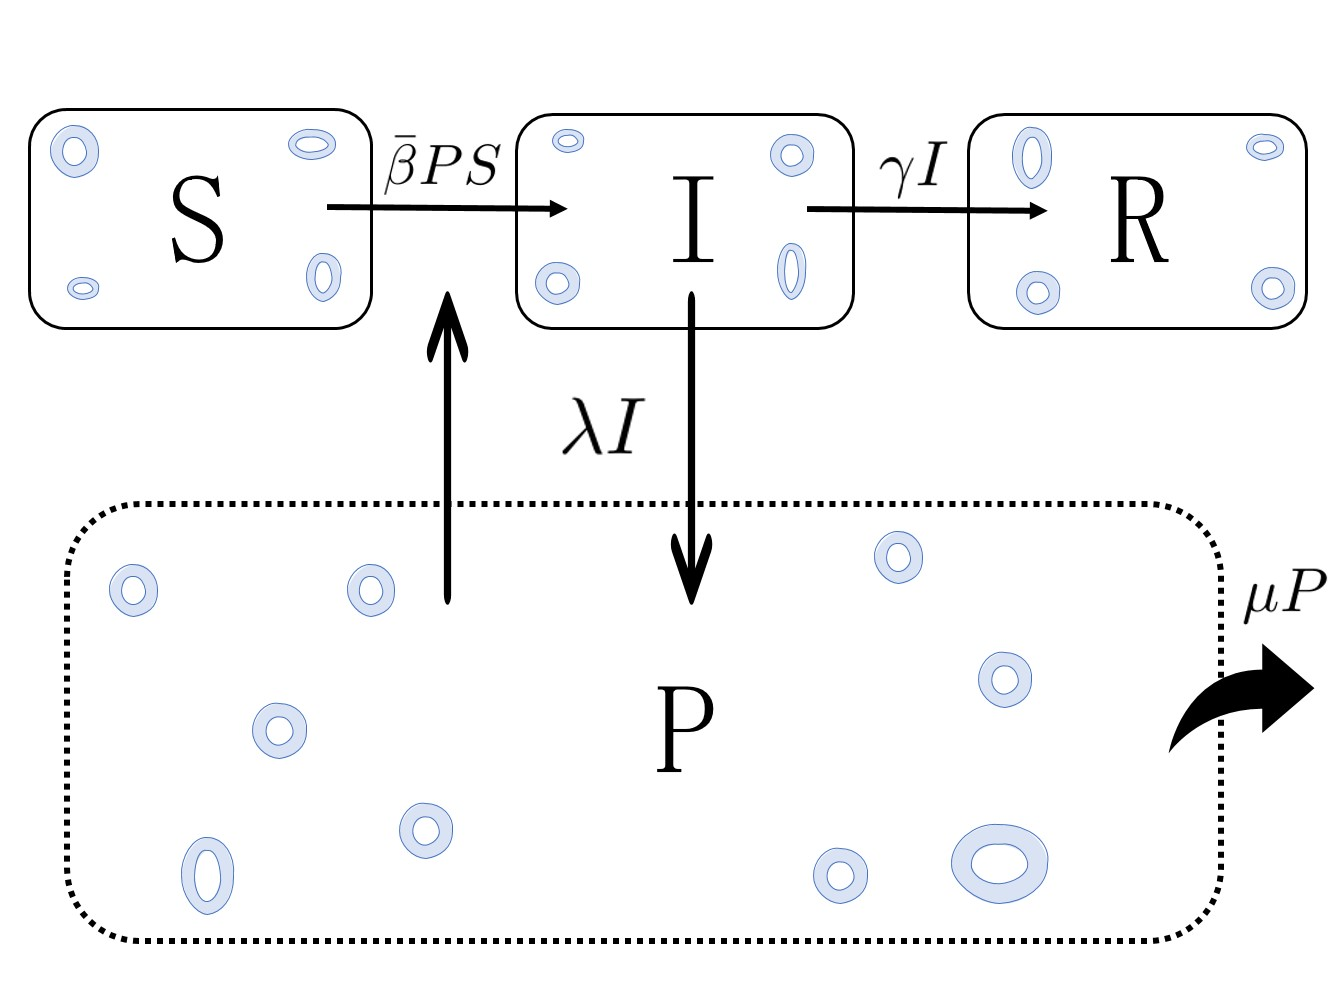
\includegraphics[width=1\textwidth]{Figures/SIRP_scheme_mod.jpg}
    \caption{SIRP model flow diagram. The model variables are represented
        by capital letters: susceptible hosts ($S$), infected hosts ($I$), dead
        hosts
        ($R$) and the population of parasite ($P$). Arrows represent the
        processes in
        the model with their rates indicated next to them and blue rings
        represent
        parasites. The flow follows the scheme in \cref{eq:scheme_reinfection},
        that
        leads to the system of differential equations in \cref{eq:SIRP}.}
    \label{fig: SIRP_scheme}
\end{figure}

\begin{table}[H]
    \centering
    \caption{Model parameters description}
    \begin{tabular}{cl:cl}
        \hline \hline
        Variable & Definition             & Parameter & Definition
        \\ \hline
        $S$      & Susceptible host       & $\beta$   & Disease transmission
        rate                                                                 \\
        $I$      & Infected host          & $\gamma$  & Host mortality rate
        \\
        $R$      & Removed host           & $\lambda$ & Production rate of
        parasites by
        infected hosts
        \\
        $P$      & Parasite in the medium & $\mu$     & Parasite
        deactivation/dilution rate
        \\ \hline \hline
    \end{tabular}
    \label{tab:parameters}
\end{table}

Following this argumentation, the scheme in \cref{eq:scheme_reinfection}
and \cref{fig: SIRP_scheme}, one can write the evolution equations of the SIRP
model,
\begin{equation}\label{eq:SIRP}
    \begin{aligned}
        \dot{S} & =-\bar{\beta} P S                    \\
        \dot{I} & =\bar{\beta} P S-\gamma I            \\
        \dot{R} & =\gamma I                            \\
        \dot{P} & =\lambda I-\bar{\beta} P S-\mu P \ .
    \end{aligned}
\end{equation}
Model (\cref{eq:SIRP})	\textit{lives} in the $4$-dimensional (S,I,R,P)
phase space, representing the variables
the populations of individuals in the susceptible, infected and removed
host compartments and of parasites, respectively. These variables could be
redefined so that S, I and R represent proportions of hosts in each compartment
and P the population of parasites per host.

The fixed points of \cref{eq:SIRP} are determined by the
conditions\footnote{We do not consider the trivial fixed point $S=I=R=P=0$ that
    would imply $N=0$ and $P=0$ at all time.}
$I=P=0$, to be fulfilled simultaneously.
We will study the stability of the fixed point defined by $S(0)$,
$I(0)=P(0)=0$ and $R(0)=N-S(0)$.
A linear stability analysis of this fixed point reveals that it has two
null eigenvalues, that stem from the condition $N=S+I+R$ and the conserved
quantity of \ref{app:P_exact}.
The first condition, $S+I+R=N$, implies that it is enough to consider two
of the host populations, e.g. $S$ and $I$, as the third one can be obtained
from the other two. The implications of the conserved quantity reported in
\ref{app:P_exact} are more subtle, as it implies that fixed points are not
isolated, as it happens in ordinary dissipative dynamical systems, and there is
an infinite number (a line of) fixed points for the final state of the
epidemic, depending on the initial conditions. This also implies that the phase
space is foliated by the conserved quantity, $C$ of
\cref{eq:conservedquantity}, and every initial condition, $S_0$, with a
different value of $C$ leads to a different asymptotic condition, $S_{\infty}$,
just as shown in \cite{Murray_book} for the SIR model (cf. Fig. 10.1 in
\textit{op. cit.}).
The third eigenvalue, that is the largest of the two non-zero eigenvalues,
can be positive if $\beta S_0 \lambda>\gamma(\beta S_0+\mu)$ and negative if
the inequality is reversed, defining the conditional stability of the fixed
point. The fourth eigenvalue is always negative and all the eigenvalues are
always real (cf. \ref{app:linstabfp}).
The instability of the fixed point along the third eigenvalue drives the
beginning of the epidemic.

An extremely important result in epidemiology is the so-called
\textit{basic reproduction number}, $R_0$, a dimensionless number which
represents the number of secondary infections produced by a primary infection
in a fully susceptible population. $R_0=1$ defines the threshold for epidemic
propagation: an epidemic will occur when $R_0>1$, and the number of infected
individuals will grow, at an exponential rate in the early phases of the
epidemic \cite{Castro2020}, while if $R_0<1$ the infection will wane
naturally.
This quantity can be formally obtained making use of the Next Generation
Matrix (NGM) method \cite{Theory_next_gen_matrix, Diekmann2010}. Applying this
formal method to our system of ordinary differential equations (ODE's) one
obtains the following relation for the basic reproduction number (cf.
\ref{app:NGM}),
\begin{equation}\label{eq:R_0_SIRP}
    R_0=\frac{\lambda}{\gamma\parentesi{1+\displaystyle\frac{\mu}{\bar{\beta}
                S(0)}}} \ .
\end{equation}

The threshold condition provided by $R_0$ (\cref{eq:R_0_SIRP}) is
equivalent
to the linear stability condition for the third eigenvalue of the initial,
pre-epidemic, fixed point, as $\bar{\beta} S(0) \lambda>\gamma(\beta S(0)+\mu)$
implies that this eigenvalue is positive and the disease-free equilibrium
state unstable being this
equivalent to $R_0>1$ (cf. \ref{app:linstabfp}).
Thus, if $R_0>1$ the fixed point is unstable, and an epidemic will ensure
if infected hosts, $I$, or parasites, $P$ appear in the system. An epidemic
will propagate until the system reaches an stable fixed point, that signals the
end of the epidemic (cf. \ref{app:linstabfp}).

\subsection{Model reduction} \label{sec:reduction}

The SIRP model lives in a $4$-dimensional phase space and depends on $4$
parameters, what makes difficult to confront it with experimental data. Thus,
we will discuss here
three alternative ways of reducing the model. The first involves an exact
reduction of the model, based on the conserved quantity derived in
\ref{app:P_exact}. The second reduction consists of an approximation to the
previous exact reduction, that turns out to be equivalent to an exact reduction
of a slightly simplified model (without the $-\bar{\beta}SP$ term in the
equation of $\dot{P}$). The third one is based on an approximation valid if the
system parameters fulfil certain conditions.

\subsubsection{Exact reduction of the SIRP model} \label{sec:exactred}

From the conserved quantity derived in	\ref{app:P_exact}, it is possible
to write the parasite population in the SIRP model as a function of the host
states as follows,
\begin{equation}\label{eq:P_exact}
    P(S,I)=-\frac{\lambda}{\gamma}\parentesi{S+I} +
    \frac{\mu}{\bar{\beta}}\ln(S) + S + C(0) \ ,
\end{equation}
where $C(0)=P(0)+\displaystyle\frac{\lambda}{\gamma}\parentesi{S(0)+I(0)} -
    \frac{\mu}{\bar{\beta}}\ln(S(0)) - S(0)$.\\

Substituting \cref{eq:P_exact} into the general SIRP model of
\cref{eq:SIRP} we obtain the following nonstandard SIR model,
\begin{equation}\label{eq:SIR_exact}
    \begin{aligned}
        \dot{S} & = \frac{\lambda\bar{\beta}}{\gamma}S\parentesi{S+I} - \mu
        S\ln(S) - \bar{\beta} S^2 - S\bar{\beta} C(0)                        \\
        \dot{I} & = -\frac{\lambda\bar{\beta}}{\gamma}S\parentesi{S+I} + \mu
        S\ln(S) + \bar{\beta} S^2 + S\bar{\beta} C(0) -\gamma I              \\
        \dot{R} & =\gamma I \ .
    \end{aligned}
\end{equation}

Although using the conserved quantity yields an exact reduction from a 4D
dynamical system to a 3D one, the number of independent parameters and initial
conditions remain unchanged, i.e. they still depend on $4$ parameters and $4$
initial conditions. Thus, although useful, (\ref{eq:SIR_exact}) is not ideal
when trying to fit experimental data, and this is the reason for trying a
further approximation to \cref{eq:SIR_exact} to be discussed next.

\subsubsection{Further approximation to the exact reduction}
\label{sec:exactredapp}

A further approximation to \cref{sec:exactred}, that is less restrictive
and expected to be valid in a broader parameter range than \cref{sec:fastslow}
is possible. This approximation reduces the number of free parameters by one,
what is useful in fitting available data.
The approximation consists of neglecting the
$S$ term in \cref{eq:P_exact}, what is possible if $\lambda/\gamma\gg 1$
and also $\mu\ln N/(\bar{\beta} N)\gg 1$, as $S(t)$ decreases monotonically
with time and is, at most, $N$ at the initial time. Interestingly, this
approximation is equivalent to the simplification of the equation for $\dot{P}$
in (\ref{eq:SIRP}) so that the $-\bar{\beta}SP$ is skipped, what yields exactly
the SIP model of Ref. \cite{article_SIP}. This reduced model has an exact
conserved quantity, $\mathcal{C}$, that differs from that of the SIRP model in
the linear $S$ term (cf. \ref{app:P_exact}).
Using this approximation one can write,
\begin{equation}\label{eq:SIR_exact_reduced}
    \begin{aligned}
        \dot{S} & =\frac{\lambda'}{\gamma}S(S+I)-\mu
        S\ln(S)-S\bar{\mathcal{C}}(0)                 \\
        \dot{I} & =-\frac{\lambda'}{\gamma}S(S+I)+\mu
        S\ln(S)+S\bar{\mathcal{C}}(0)-\gamma I        \\
        \dot{R} & =\gamma I \ ,
    \end{aligned}
\end{equation}
where $\lambda'=\lambda\bar{\beta}$ and $\bar{\mathcal{C}}(0)=\bar{\beta}
    (P(0)+\lambda/\gamma(S(0)+I(0)-\mu/\bar{\beta}\ln S(0)))=\bar{\beta}
    \mathcal{C}(0)$ is a redefinition of the conserved quantity of the SIP
model
\cref{eq:conservedquantitySIP}, $\mathcal{C}(0)$, a constant, such that it
absorbs $\bar{\beta}$ and all initial conditions of the model. The result is
that \cref{eq:SIR_exact_reduced} depends on $3$ parameters and $1$ constant,
compared to \cref{eq:SIR_exact} that depends on $4$ parameters,
facilitating, thus, the use of the model to fit experimental data.

\subsubsection{Model reduction through fast-slow separation}
\label{sec:fastslow}

The third
reduction of the $4$-D dynamical model \cref{eq:SIRP} makes the assumption
that
the time scale in which the parasite population changes are faster than the
one corresponding to the host. This means that pathogen deactivation in the
medium must be faster than host mortality. In terms of the rates associated to
each of these processes, this means $\mu>\gamma$. Taking $\mu$ as common factor
in $\dot{P}$ one can write,
\begin{equation}
    \epsilon \dot{P} =\lambda I/\mu-\bar{\beta}SP/\mu-P
\end{equation}
where $\epsilon=1/\mu$ is small, as $\mu$ is large. If furthermore
$\mu\gg\bar{\beta}N$ and  $\lambda\gg \beta P$ one arrives to,
\begin{equation}\label{eq:P_approx}
    P\approx \frac{\lambda}{\mu} I \ .
\end{equation}

Under this approximation the slow subsystem can be written,
\begin{equation}\label{eq:SIRslow}
    \begin{aligned}
        \dot{S} & =-\beta' I S         \\
        \dot{I} & =(\beta' S-\gamma) I \\
        \dot{R} & =\gamma I\ ,
    \end{aligned}
\end{equation}
that is equivalent to the classical SIR model with $\beta'=\bar{\beta}
    \lambda/\mu$ instead of the infection rate $\bar{\beta}$. The reduced $3$-D
model \cref{eq:SIRslow} from the original $4$-D SIRP model \cref{eq:SIRP}
depends on $2$ parameters instead of $4$ as the original model had and $1$
initial condition, e.g. $I(0)=N-S(0)$ if $R(0)=0$, and is much more amenable to
be applied to the analysis of experimental data, as shown in
\cref{sec:validation}.
Furthermore, $\gamma$ could be eliminated through a time rescaling,
$t\rightarrow=t'=\gamma t$ with a redefinition of
$\beta'\rightarrow\beta''=\beta'/\gamma=\beta\lambda/(\mu\gamma)$, leaving the
model as a function of a single effective parameter. However, we will keep both
$\beta'$ and $\gamma$ for convenience when fitting the model to experimental
data in \cref{sec:validation}, as we would need to know anyhow $\gamma$ in
order to analyse the experimental data. The validity of this approximation is
checked numerically in \cref{sec:numericalanalysis}.

\section{Numerical analysis of the model} \label{sec:numericalanalysis}

Due to the impossibility of solving the SIRP model analytically,
in the present section we perform a numerical characterisation of the
model\footnote{All numerical simulations of the dynamical system
    \cref{eq:SIRP} have been carried out using a Runge-Kutta $4$th order
    method,
    with a temporal step $\Delta t=0.001$. Numerically stable results are
    obtain
    with $\Delta t\le 0.01$.}.
Moreover, we show the validity range of the performed approximations to
reduce the SIRP model to an effective SIR model. We start our numerical
analysis by investigating the relative influence of the model parameters on
some epidemiological quantities of interest: the basic reproduction number
($R_0$), related to the existence of an epidemic outbreak, continuing with the
final state of the epidemic, given by the final number of dead individuals
($R(\infty)$) and the maximum of infected individuals ($I_{\textrm{max}}$)
together with the time at which it occurs ($t_{\textrm{max}}$).

In order to identify the most influential parameters of our model
Sensitivity Analysis (SA) will be performed. SA can be divided into two
classes: Local Sensitivity Analysis (LSA) and Global Sensitivity Analysis
(GSA). LSA represents the assessment of the local impact of input factors
variation on model response by concentrating on the sensitivity in the vicinity
of a set of factor values. Such sensitivity is often evaluated through
gradients or partial derivatives of the output functions at these factor
values, such that other input factors are kept constant.
Since epidemic models exhibit a threshold behaviour, controlled by the
dimensionless quantity
$R_0$, it is relevant to study its robustness with respect to small
perturbations by means of the LSA explained above, as its analytical expression
is known.

On the other hand, GSA will be applied to study the influence of the
parameters in the final state of the epidemic and the epidemic peak by
exploring a large domain of the parameter space. In turn, GSA is the process of
apportioning the uncertainty in outputs to the uncertainty in each input factor
over their entire range of interest. A sensitivity analysis is considered to be
global when all the input factors are varied simultaneously and the sensitivity
is evaluated over the entire range of each input factor, in clear contrast to
LSA. Within GSA, first order indices are a measure of the contribution to the
output variance given by the variation of the parameter alone averaged over
variations in other input parameters while second order indices take into
account first order interactions between parameters. While LSA is carried out
analytically (if exact expressions are available), GSA is a purely numerical
approach. Further mathematical details on Sensitivity Analysis can be found in
\ref{app:sensanal}.

For all the sensitivity analysis performed in the following sections, and
in order to avoid ambiguities associated to the definition of $\bar{\beta}$ as
a function of $N$, we assume $N=1$, so that both possible incidences yield
$\bar{\beta}=\beta$ and the numerical results are equivalent.

\subsection{The basic reproduction number $R_0$}

To study the relevance of parameters involved in an epidemic outbreak a LSA
was performed. We analyse the local sensitivity of $R_0$ through the normalised
sensitivity index, so that the function $F(\vec{p})$ of
\cref{eq:sensitivity_analysis} is substituted by the analytical expression of
$R_0$, \cref{eq:R_0_SIRP}.

\cref{fig:Local_Sensitivity_Analysis_R0}(a) shows the sensitivity index for
$R_0$ for specific baseline parameters, where $\lambda$, $\bar{\beta}$ and
$S_0$ contribute to increase the basic reproduction number while $\alpha$,
$\gamma$ and $\mu$ contribute to decrease it, as expected. Moreover, we can see
that $\lambda$ and $\gamma$ are the most influential parameters while $\mu$,
$\bar{\beta}$ and $S_0$ depend on each other. These dependencies cause varying
influences on $R_0$, which are fully depicted in panels
\cref{fig:Local_Sensitivity_Analysis_R0}(b-d). It can be seen that the
influence of $\bar{\beta}$ increases with the increase of $\mu$ and the
decrease of $S_0$. Similarly, the importance of $S_0$ increases with $\mu$ and
decreases with $\bar{\beta}$. On the other hand, the impact of $\mu$ increases
with the decrease of both $S_0$ or $\bar{\beta}$.

\begin{figure}[H]
    \centering
    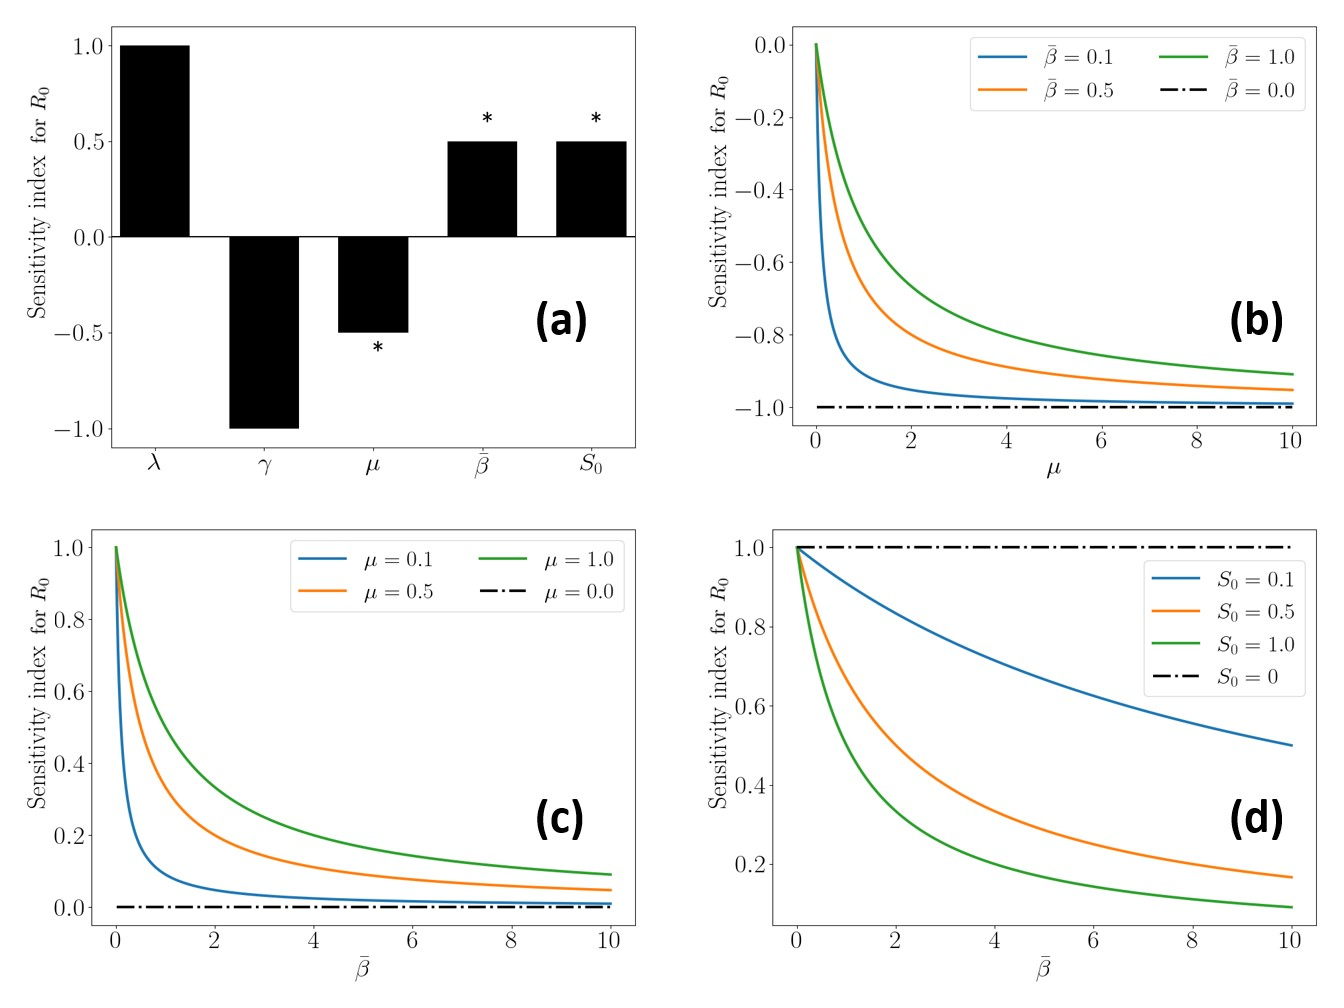
\includegraphics[width=1\textwidth]{Figures/R_0_sensitivity.jpg}
    \caption{Panel (a): Local sensitivity analysis of $R_0$ for the
        baseline parameters $\lambda=1$, $\gamma=1$ and
        $\mu=\bar{\beta}=S_0=1$. The
        asterisks mark parameters for which the sensitivity index is not
        constant,
        depending on, at least, another parameter. Panels (b-d): Local
        sensitivity
        analysis of $R_0$ with respect to parameters with an asterisk, showing
        the
        different dependence with a second parameter and the effect on the
        varying
        sensitivity index.}
    \label{fig:Local_Sensitivity_Analysis_R0}
\end{figure}

\subsection{Final state of the epidemic}

Another important quantity in epidemiology is the final state of the
epidemic, which can be characterised by the final number of dead individuals,
$R_\infty$. Within our general SIRP model it is not possible to find an
analytical expression of $R(t)$ so that we need to tackle the problem
numerically. To this end, we perform GSA for the final number of dead
individuals in order to determine the most influential parameters for this
quantity. In particular, we apply the Sobol method, discussed in
\ref{app:sensanal}.
The Confidence Interval, CI, obtained in our
study is less than 1\% of the index value, indicating a very high accuracy,
therefore it is not shown in the figures. The results of the explained
procedure are shown in \cref{fig: GSA_R_inf}, where the total order (black),
first order (white) and second order (gray) sensitivity indices for each of the
model parameters are detailed. It can be observed that $\mu$ has a slightly
greater influence than the other parameters with respect to the final number of
dead individuals. Note that the second order indices are larger than the first
order ones for all the parameters, which indicates a high influence of the
nonlinearities in our model, at least for the particular quantity under study.

\begin{figure}[H]
    \centering
    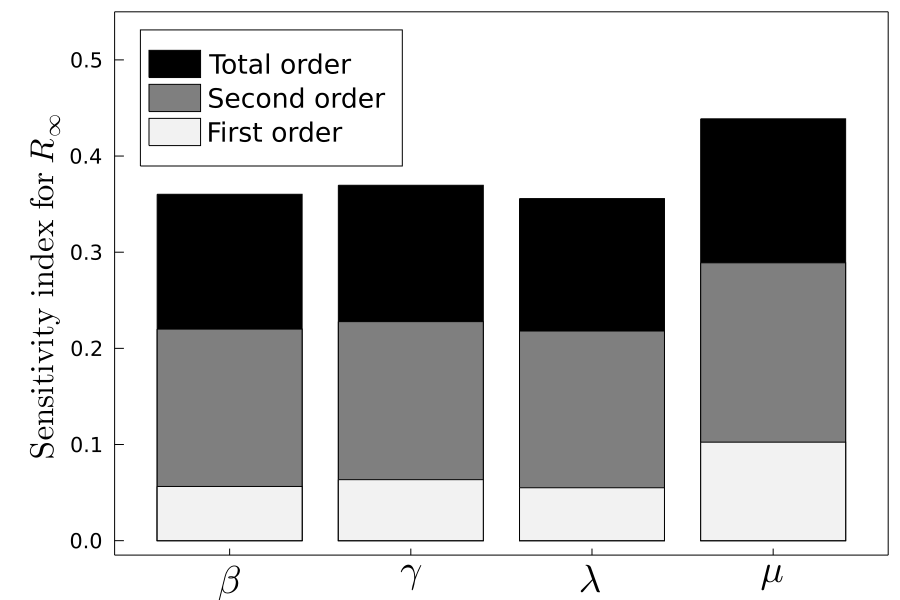
\includegraphics[width=0.7\textwidth]{Figures/GSA_R_inf.png}
    \caption{Sensitivity indices (LSA) for the final number of dead
        individuals ($R_\infty$) for each one of the indicated parameters. The
        black
        bars represent the total order indices of sensitivity while white
        (grey) colour
        represents the contribution of the first (second) order indices.}
    \label{fig: GSA_R_inf}
\end{figure}

\begin{figure}[H]
    \centering
    \subfigure[Epidemic
        peak]{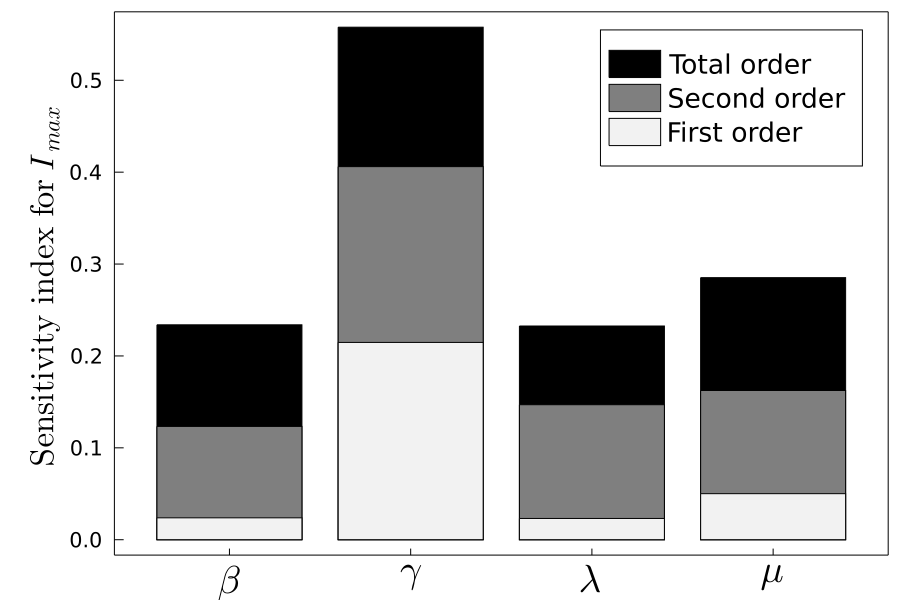
\includegraphics[width=0.49\textwidth]{Figures/GS_peak.png}}
    \subfigure[Time of epidemic
        peak]{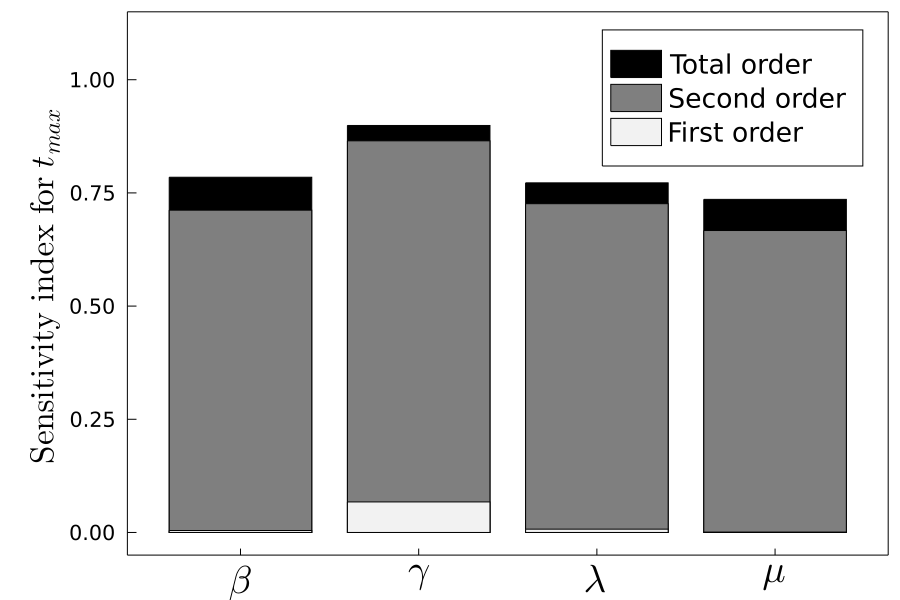
\includegraphics[width=0.49\textwidth]{Figures/GS_peak_time.png}}
    \caption{Global sensitivity analysis for the maximum of infected
        individuals $I_{\textrm{max}}$ (a) and its time occurrence
        $t_{\textrm{max}}$
        (b). The black bars represent sensitivity at all orders,
        while white (grey) colour represents the contribution of the first
        (second) order indices.}
    \label{fig: GS_analysis}
\end{figure}

\subsection{Maximum of infected individuals}

A GSA of the maximum number of infected individuals, $I_{\textrm{max}}$ and
the time it occurs, $t_{\textrm{max}}$ is performed to study the influence of
the model parameters regarding these quantities. In this case, \cref{fig:
    GS_analysis}, $\gamma$ has greater influence in the epidemic peak than any
of
the other parameters, while for the time at which the peak takes place, all the
parameters have basically the same influence. Again, the second order indices
(the first order interactions between parameters) account for most of parameter
sensitivity, in particular in the time of the epidemic peak, indicating the
high degree of nonlinearity of this effect.

\begin{figure}[H]
    \centering
    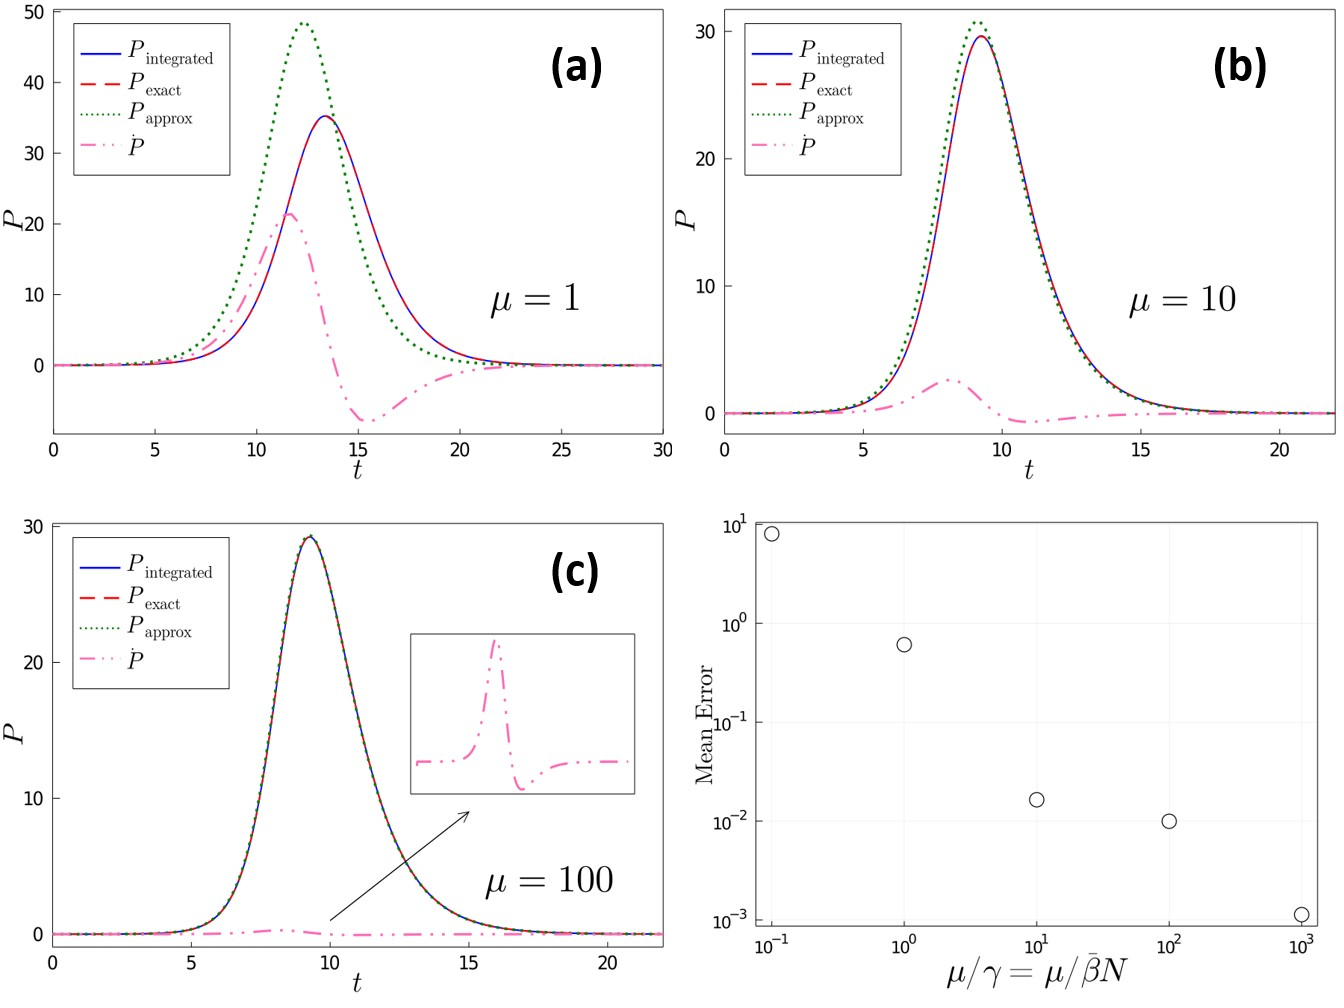
\includegraphics[width=1\textwidth]{Figures/P_comparison.jpg}
    \caption{Numerical check of the approximate expression for the pathogen
        concentration, (\cref{eq:P_approx}), $\bar{\beta}=1/50$ and $\gamma=1$:
        (a)
        $\mu=1$; (b) $\mu=10$; (c) $\mu=100$, while $\lambda$ is varied to keep
        $R_0=2.5$, defined in (\cref{eq:R_0_SIRP}) (with $S_0=N=50$), i.e.,
        $\lambda=5,
            27.5, 252.5$ respectively for (a)-(b)-(c), respectively.
        The blue solid line represents the numerically integrated quantity, the
        red dashed line (superimposed to the blue solid one as they are
        identical) is
        the exact solution for this quantity, (\cref{eq:P_exact}) and the green
        dotted
        line accounts for the approximate expression from the timescale
        separation
        (\cref{eq:P_approx}). The dash-dotted pink line represents the
        derivative of
        $P$, $\dot{P}$, in the scaled time frame. Panel (d): Mean error between
        the
        approximate and exact solutions for increasing
        $\mu/\gamma=\mu/\bar{\beta}$.}
    \label{fig:P_comparison}
\end{figure}

\subsection{Numerical verification of the fast-slow approximation}

The parasite concentration approximation, based on a timescale separation
discussed in \cref{sec:fastslow}, is now verified by computational means. The
verification was performed using both mass action and standard incidence, but
for the sake of simplicity we show only the results for the standard incidence
case. Worth is to say that, mathematically, changing from standard incidence to
mass action involves only a rescaling of the $\beta$ parameter, so that the
numerical results are exactly the same. \cref{fig:P_comparison} contains a
comparison for $3$ different values of the parasite deactivation rate, $\mu$.
It can be seen that the approximation is poor when $\mu\sim
    \gamma,\bar{\beta}N$ \cref{fig:P_comparison}(a), as it could be expected.
On
the other hand, the approximation is quite good when $\mu$ is one order of
magnitude larger than $\gamma$ and $\bar{\beta}N$ \cref{fig:P_comparison}(b),
while it is extremely accurate when $\mu$ is two orders of magnitude larger
than $\gamma,\bar{\beta}N$, \cref{fig:P_comparison}(c). The figure also shows
the numerical value of $\dot{P}$ (pink dashdot), and it can be checked how it
becomes smaller as $\mu$ increases compared to $\gamma,\bar{\beta}N$,
justifying the timescale separation of \cref{sec:fastslow}. Finally,
\cref{fig:P_comparison}(a-c) also shows (dashed red line) the analytical value
for $P(S,I)$ derived in \cref{eq:PSI_exact}, that matches perfectly the result
of the numerical integration of \cref{eq:SIRP}, as should be the case.

\begin{figure}[H]
    \centering
    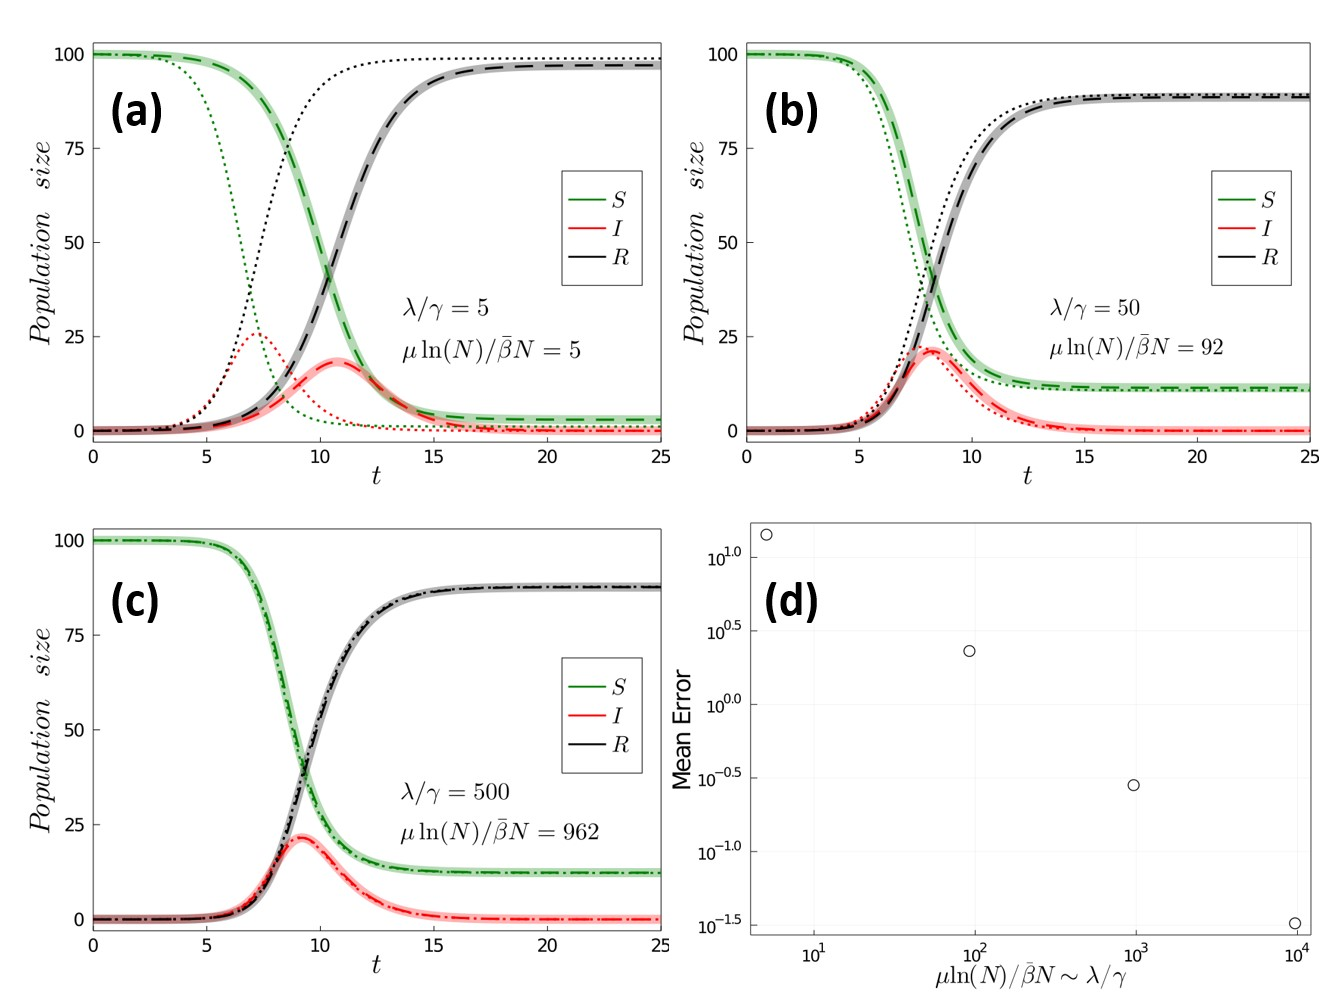
\includegraphics[width=1\textwidth]{Figures/exact_reduction_approx.jpg}
    \caption{Numerical check of the exact model reduction along with the
        subsequent approximation shown in \cref{sec:exactred} with $N=100$,
        $\bar{\beta}=1/100$, $\gamma=1$, (a) $\lambda=5$, $\mu=1.1$; (b)
        $\lambda=50$,
        $\mu=20$; (c) $\lambda=500$, $\mu=209$. $R_0=2.38$ for all the panels.
        The
        solid semitransparent lines represent the original 4D model, the dashed
        lines
        the exact reduction and the dotted lines the approximate model from the
        exact
        reduction. Panel (d): Mean error between the approximate and exact
        solutions
        for increasing $\mu\ln(N)/\bar{\beta}N$ and $\lambda/\gamma$ while
        $R_0=2.38$
        is kept constant.}
    \label{fig:verification_exact_reduction}
\end{figure}

\subsection{Numerical verification of the model approximation from the
    exact reduction} \label{sec:apprexred}

The numerical verification was performed for both mass action and standard
incidence, but for the sake of simplicity in
\cref{fig:verification_exact_reduction} we show only the results for the
standard incidence case. First, and as it should be because it is an exact
result, the exact reduction of the SIRP model discussed in \cref{sec:exactred}
matches perfectly the numerical results obtained from the full model for all
possible parameter values,
\cref{fig:verification_exact_reduction}(a-c).
Regarding the approximation to the exact reduction, one can see
how the approximation converges to the exact solution as the parameters
fulfil the conditions indicated in \cref{sec:exactredapp}, namely that both
$\gamma/\lambda\gg 1$ and $\mu\log(N)/\bar{\beta N}\gg 1$, becoming very
accurate if these ratios are larger than $1$ by two orders of magnitude or more
(cf.  \cref{fig:verification_exact_reduction}(c)). We recall that in this case
the SIRP model converges to the SIP model of \cite{article_SIP}. Conversely,
the approximation is poor when any of these two ratios is of order $1$ ((cf.
\cref{fig:verification_exact_reduction}(a))), while
\cref{fig:verification_exact_reduction}(b) presents the result in an
intermediate case, in which the approximation is fair.

\section{Model validation with data of the \textit{Pinna nobilis} Mass
  Mortality Event}
\label{sec:validation}

In this section, the general SIRP model is validated against collected data
from the \textit{Pinna nobilis} Mass Mortality Event. As explained in
\cref{sec:Introduction_Nacras_I}, the disease is caused by the parasite
\textit{Haplosporidium pinnae} and the hosts, \textit{P. nobilis}, are sessile
bivalves endemic of the Mediterranean Sea. Thus, this epidemic is a perfect
candidate to be described by the SIRP model. In the model, parasite production
occurs only inside infected hosts, and parasites are released to the medium,
either through their respiratory or digestive system. The simultaneous
occurrence of the different possible stages of the parasite (uni- and
bi-nucleate cells, multinucleate plasmodia, sporocysts and uninucleate spores)
in the same host individual is not common among haplosporidans and makes
\textit{H. pinnae}  different from previously known haplosporidan species
\cite{CATANESE20189}. The occurrence of uni- and binucleate stages suggest
possible direct transmission from infected to healthy fan mussels, as observed
in \textit{B. ostreae} and \textit{B. exitiosa} \cite{hine1996ecology,
    Culloty2007, Audemard2014}. Additionally, the presence of spores (a
dormant,
resistant stage) could allow long persistence in the environment and the
hypothetical involvement of an intermediate host as suggested for \textit{H.
    nelsoni} and \textit{H. costale} \cite{Andrews1984,
    haskin1988uncertainties,
    powell1999modeling}. While uninucleate cells are always detected in
infected
fan mussels, sporulation has been only detected sporadically
\cite{CATANESE20189}. Thus, we assume that infection occurs mostly through
uninucleate (or binucleate) cells by direct transmission (as the experimental
observations in captivity point out, see \cite{March}).
We do not consider disease transmission through other stages. We do not
consider spores, given the infrequent observation of spores and the current
lack of experimental information about spore transmission (that could involve
another intermediate host species). Regarding plasmodia and sporocyst stages,
these stages are too large to be released through the epithelium. The
distinction between uninucleate and binucleate cells seems unnecessary at this
level of representation, as these phases only participate in parasite
proliferation inside infected hosts, a process that we consider in an effective
way. Finally, the evidence of the time course of the disease compared to the
long life cycle of {\it P. nobilis\/} suggests host vital dynamics (i.e.
recruitment (reproduction) and natural death) can be neglected.

After an epidemic outbreak that took place in Portlligat, in the north east
of Catalonia, $215$ \textit{Pinna nobilis} individuals were extracted from
their natural medium in order to be preserved as a genetic reserve in several
controlled water tanks of different institutions in Spain \cite{March}. The
institutions that participated in this preservation effort were IFAPA, IEO,
IRTA, IMEDMAR-UCV and Oceanogr\`afic of Valencia. The original idea was to
rescue the individuals before infection, however, the subsequent evolution of
the rescued \textit{Pinna nobilis} populations indicates that some individuals
were already infected at the time of extraction (and/or in contact with some
amount of the parasite transferred from sea water).
This allowed the opportunity to use the data of the time evolution of the
epidemic in the controlled water tanks, reported in \cite{March}, to evaluate
the described SIRP model\footnote{Data use in this work with the purpose of
    validating and fitting parameters for the SIRP model have been taken from
    the
    Supplementary Information of \cite{March}}. The empirical data consists of
the
proportion of survivors as a function of time in the controlled water tanks
with a temporal resolution of one month. Despite the fact that the temperature
of the water in the tanks was controlled, it was sharply lowered in most of the
tanks when mortality started to appear within the population, as a last effort
to keep the rest of the population safe and alive, since keeping the
temperature below  approximately $13.5\, {}^o$C is a known strategy to preserve
\textit{Pinna nobilis} individuals as disease expression is minimal
\cite{Cabanellas2019}. Fortunately, two of the tanks kept its temperature
approximately constant during the full recorded time. This is the case of the
tanks in IFAPA in Huelva and the Oceanogr\`afic of Valencia (OCE), both Spanish
institutes. These water tanks have been selected to validate our model,
maintaining constant temperatures of $14\, {}^o$C and $17\, {}^o$C,
respectively.

First we will fit the exact reduction of the SIRP model, assuming
$\mu\log(N)\gg\bar{\beta}N$ and $\lambda/\gamma\gg 1$ as discussed in
\cref{sec:exactredapp}, namely \cref{eq:SIR_exact_reduced}.
This reduced model depends on three parameters ($\lambda'$, $\mu$,
$\gamma$) and one constant, $\bar{\mathcal{C}}(0)$, cf. \cref{sec:exactredapp},
that is related to the initial conditions of the model. The order of magnitude
of the mortality rate can be deduced from data, with an estimate value of
$\gamma\approx\SI{1}{month^{-1}}$. We fix this parameter in order to give some
biological information to our model prior to the computational fit. We focus on
the $R$ compartment, as it can be retrieved directly from data in
\cite{March}\footnote{The number of dead individuals can be obtained as
    $R=N-S$, where $S$ is the population of survivors and $N$ is the total
    number
    of individuals in the tanks,
    $50$ (IFAPA) and $5$ (Oceanogr\`afic), respectively}.
We use a box-constrained variant\footnote{We constrain the optimisation
    because the unconstrained optimisation to the full range of the parameters,
    i.e, from $0$ to $\infty$ is not practical.} of the well known BFGS
optimisation algorithm \cite{BFGS} with a common $\textrm{L}2$ loss function,
also known as Residual Sum of Squares (RSS)\footnote{The algorithm is
    implemented within the Julia high-level programming language \cite{julia}
    using the DifferentialEquations.jl package
    \cite{DifferentialEquations.jl}.}.
By running this algorithm one observes that the optimal parameters tend to be
the ones in the boundary of the box-constrained parameter space.
Furthermore, if the box size is increased (or decreased) the optimal
parameters continue to be in the boundary of the box-constrained parameter
space.
This indicates that there exist several parameter combinations that
optimally fit the data, and the combination parameters found by the
optimisation algorithm are only marginally optimal with respect to other
parameter values. The locus (actually a valley) of marginal optimal parameters
can be seen in the right hand side panels of \cref{fig: exact_SIR_fit}, where
the cost function value of the optimisation algorithm is plotted as heat map.

\begin{figure}[H]
    \centering
    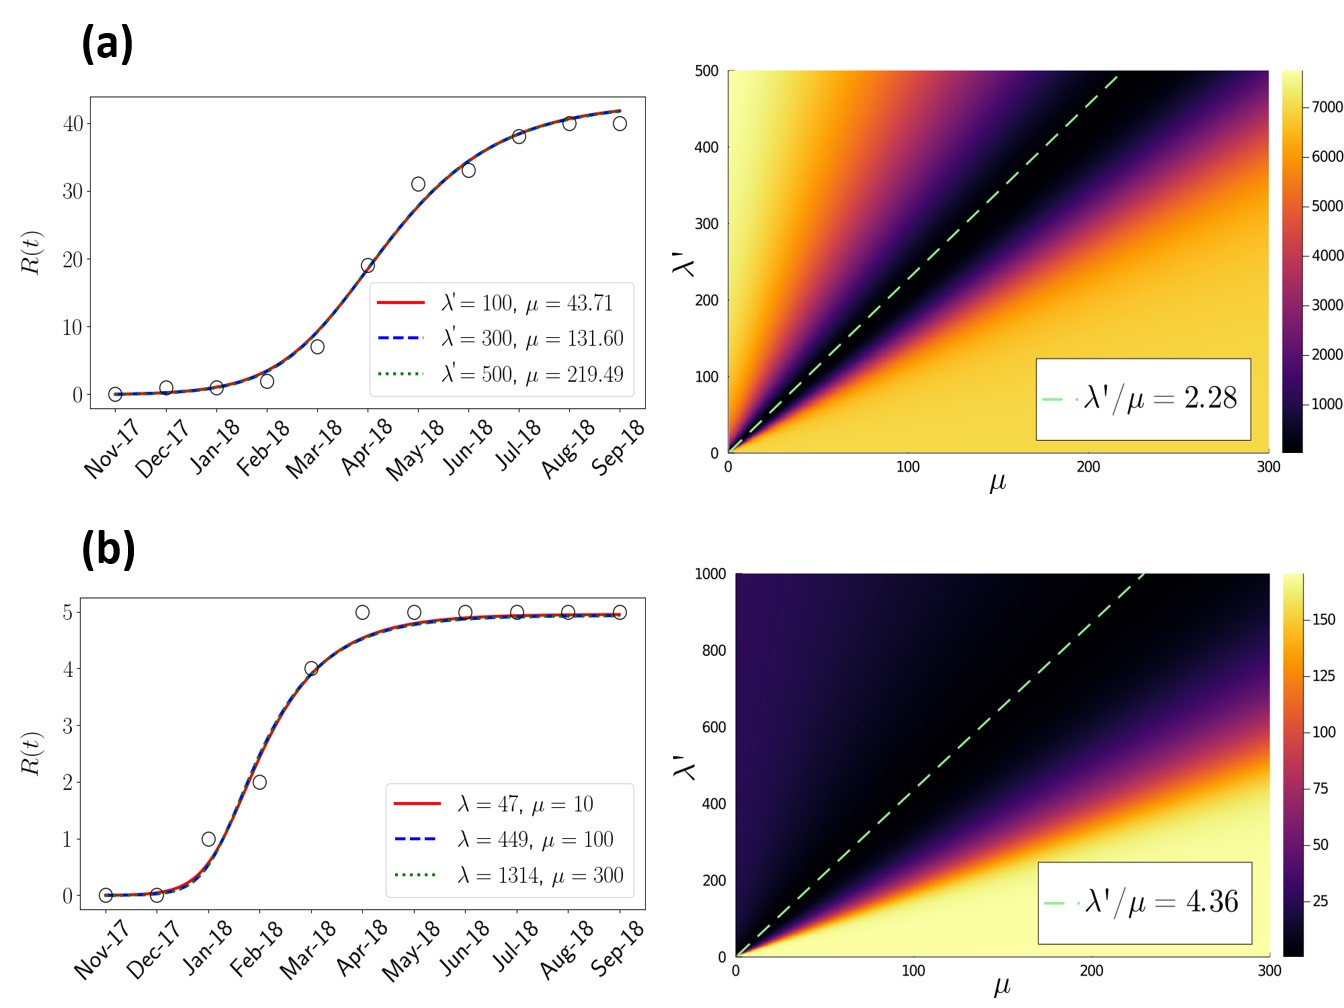
\includegraphics[width=1\textwidth]{Figures/exact_SIR_fitting.jpg}
    \caption{Parameter estimation for the approximation from the exact
        reduction of the SIRP model (\cref{eq:SIR_exact_reduced}) using data
        from IFAPA
        (panel (a)) and OCE (panel (b)) water tanks, at $\SI{14}{\degree C}$
        and
        $\SI{17}{\degree C}$ respectively. Left figures represent several fits
        of the
        model to empirical data of the number of dead hosts ($R(t)$) using
        different
        optimal combinations of the parameters. Right figures are the RSS
        errors as a
        function of the input parameters, where the green dashed line
        represents the
        set of optimal combinations of the parameters with $RSS=60, 0.8$ for
        IFAPA and
        OCE, respectively.}
    \label{fig: exact_SIR_fit}
\end{figure}

Now we reach the point regarding the dilemma between mass action and
standard incidence discussed in \cref{subsec:modtruct}. If one does not correct
the $\bar{\beta}$ parameter with the size of the host population, $N$, that is
equivalent to assuming the mass action incidence $\bar{\beta}=\beta$, the
values that one would obtain for $\beta'=\beta\lambda/\mu=\lambda'/\mu$ for
both populations take disparate values in both tanks: $\beta'=0.046$ for the
IFAPA data set and $\beta'=0.87$ for the Oceanogràfic (OCE) data set, a factor
of $19$ between them while their temperatures differ only by $3\,{}^o$C.
These numbers indicate that the standard incidence is more reasonable, what
amounts to choosing $\bar{\beta}=\beta/N$, where the final values of the
reported parameter $\beta'$ should be multiplied by $N=50$ for the IFAPA tank
and $N=5$ for the OCE tank. The final result is then $\beta'=2.28$ and
$\beta'=4.36$ for IFAPA and OCE tanks, that are the values reported in
\cref{fig: exact_SIR_fit}, implying that an almost twofold increase of the
$\beta'$ parameter corresponds to an increase of $3\,{}^o$C. This relation is
in good agreement with the typical changes in rates of a wide range of
organisms with a $\SI{3}{\degree C}$ change in temperature, while a 19-fold
change in the rate would imply at least a $\SI{30}{\degree C}$ change in
temperature (cf. \ref{app:rate_change}).

The fact that there is an infinite number of combinations of the parameters
that optimally fit the real data suggests that, as two parameters are slaved
one to each other, that the model
admits a further reduction. This reduction corresponds exactly to the
approximate $SIR$ model derived in \cref{eq:SIRslow}, with the relationship
$\beta'=\lambda'/\mu$, as anticipated. So, this gives further corroboration to
the use of the $SIR$ model \cref{eq:SIRslow} to fit $\beta'$ as the free
parameter (fixing the value of $\gamma$ and with $I_0$ as the initial condition
determined by the fit). For consistency with the previous fitting we expect to
obtain $\beta'=2.28$ and $4.36$ as the optimal parameters for the IFAPA and OCE
water tanks, respectively, and this is the case.

Interestingly, as reduced model \cref{eq:SIRslow} has fewer parameters to
fit we can relax our initial assumption of $\gamma=\SI{1}{month^{-1}}$ and
check how the fit improves or worsens when varying $\gamma$.
In \cref{fig:approx_SIR_fit} a fit of the reduced SIR model
\cref{eq:SIRslow} is shown for the IFAPA (top) and Oceanogràfic (bottom)
controlled water tanks\footnote{The $N$ correction corresponding to standard
    incidence has already been applied to these values.}.
\cref{fig:approx_SIR_fit}(c-d) shows the $RSS$ error as $\gamma$ is varied.
It can be seen that for the IFAPA water tanks $\gamma=\SI{1.5}{month^{-1}}$
yields more accurate results, while for the Oceanogràfic water tanks
$\gamma=\SI{1}{month^{-1}}$ remains optimum. This shows a decrease in the mean
removal time $1/\gamma$ for lower water temperatures, with the finite size
errors inherent to the OCE tank (as $N=5$).
In the left panels the simulated curve of dead individuals, $R$
compartment, as a function of time for the optimal fitted parameters is
confronted to the experimental data, showing a remarkable agreement. With the
optimum values of $\gamma$, in the IFAPA tank (now with
$\gamma=\SI{1.5}{month^{-1}}$) a new value of $\beta'=3.05$ is obtained,
implying a probably more reasonable ratio of $1.43$ for $\beta'$ in both tanks
(it was $1.91$ in the original fit).
From the optimal parameters we obtain the basic reproduction number, since
$R_0=\beta'/\gamma$ we have that $R_0^{\textrm{IFAPA}}\simeq2$ and
$R_0^{\textrm{OCE}}\simeq4$, clearly above the epidemic threshold.

\begin{figure}[H]
    \centering
    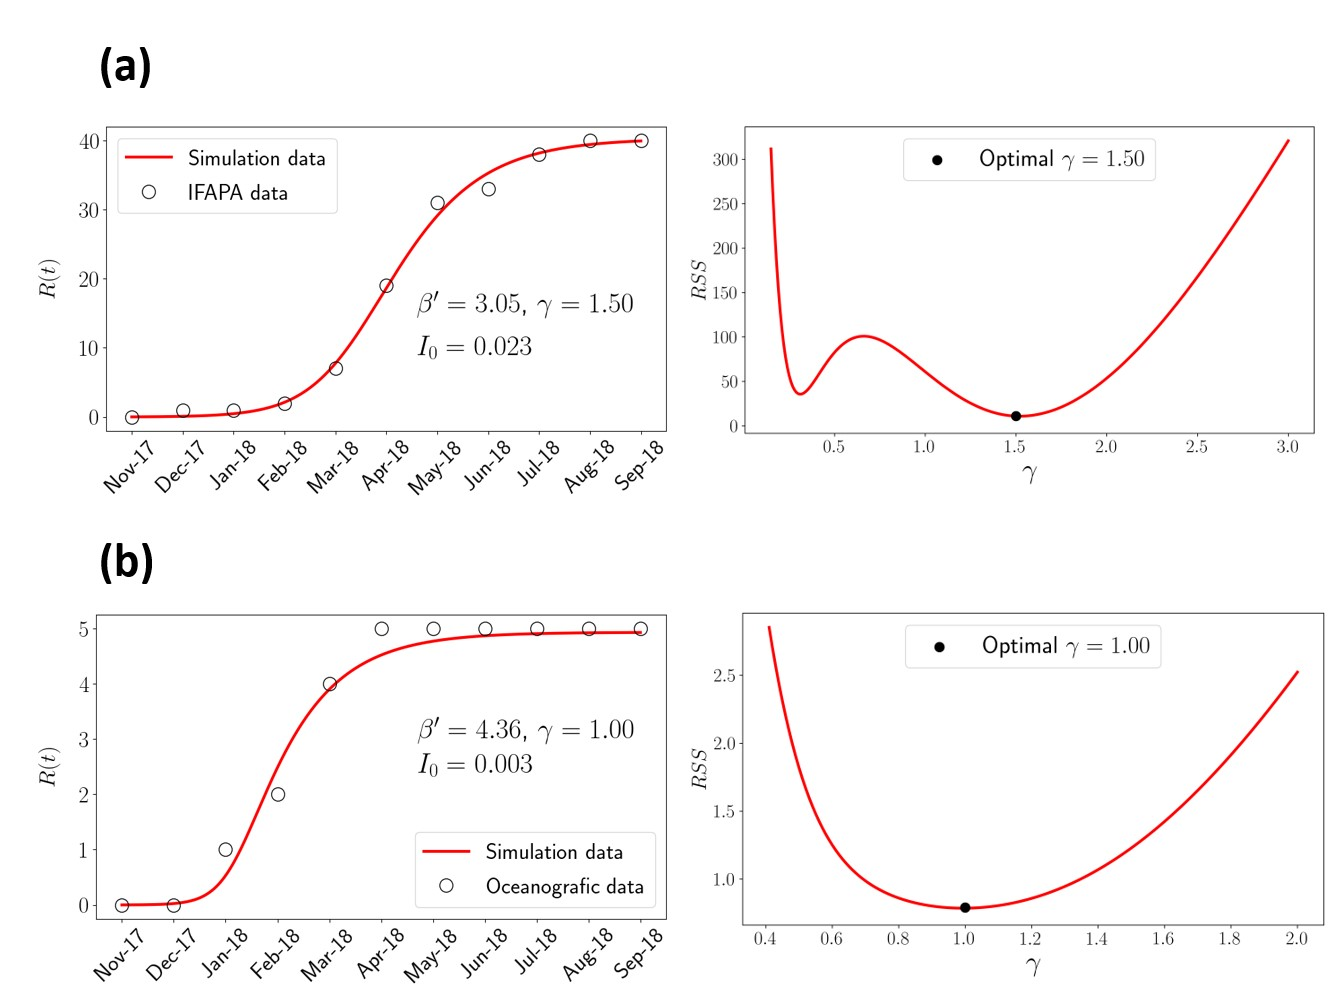
\includegraphics[width=1\textwidth]{Figures/approx_SIR_fitting.jpg}
    \caption{Parameter fitting for the R compartment to model
        (\cref{eq:SIRslow}) using data from IFAPA (panel (a)) and Oceanogràfic
        (panel
        (b)). The left part of both panels of the figure shows the optimal fit
        of the
        model to empirical data with $RSS=10.9, 0.8$ for IFAPA and OCE,
        respectively.
        The right panels show the variation of the $RSS$ error for some values
        of
        $\gamma$.  The $\beta'$ values have been obtained assuming a standard
        incidence, as explained in the main text.}
    \label{fig:approx_SIR_fit}
\end{figure}

Summarising, the SIRP model is able to fit two sets of experimental data,
agreeing with a standard incidence, according to which the infection rate
depends on the amount of parasites per pen shell individual. \textit{Pinna
    nobilis} individuals in
the IFAPA experiment were actually distributed in $4$ tanks, and the
standard incidence is compatible with this experimental aspect. The temperature
dependence of the fitted parameters in this range ($14-17 {}^o C$, appears to
be compatible (although experiments at different temperatures would be needed)
with an Arrhenius dependence of the infection parameters, also known as
Boltzmann-Arrhenius
\cite{Brown2004,Molnar2017}, that can be extended to account for the
expect unimodal dependence on temperature, with a maximum infectivity at a
characteristic temperature for the parasite \cite{Molnar2017}. Therefore, we
can assume that global change (or temperature shifts) is expected to have
complex effects on infectious diseases, causing some to increase, others to
decrease, and many to shift their distributions \cite{Rohr2020}.
In the particular case of pen shell mortality, our model results suggest the
proposed mechanism of lower disease expression at lower temperatures. This
might have direct consequences for the development of the mortality event and
offers a bleak perspective for the future and specifically in the eastern
Mediterranean basin, where the mortality was observed later due to current
patterns but average temperatures tend to be higher than in the western part of
the Mediterranean.

\section{Conclusions} \label{sec:conclusions}

In this work we have analysed a compartmental model to study marine epizootics
for sessile hosts assuming infection by direct transmission through waterborne
parasites. Moreover, we have used data from the recent mass mortality event of
\textit{Pinna Nobilis} in the Mediterranean Sea as a case study to validate our
model. Compartmental models are routinely used in the study of disease
infection and propagation in terrestrial ecosystems, including the study of the
current Covid-19 pandemic (see, e.g., \cite{Castro2020}). However, these
models are starting to be used only recently in the study of marine epizootics
\cite{article_SIP}, while proliferation models have been the most popular in
the field \cite{Powell2015}. A reason for
the low popularity of compartment models in the study of marine epizootics is
that there are some aspects in its modelling that differ from the now standard
application to terrestrial ecosystems \cite{MCCALLUM_intro}. An important
difference is that, in principle, (micro)parasites need to be modelled
explicitly in marine ecosystems, while often they are not included in the
description in terrestrial ecosystems  \cite{May1979}.

The SIRP model has $4$ compartments and depends on $4$ parameters, so that it
is not quite amenable to theoretical analysis. At the same time, due to the
large number of parameters of the model, using it to analyse experimental
observations can be cumbersome in practice if the parameter values are unknown.
Nevertheless, we have shown three reductions of the model, one exact and two
approximate ones, that can be useful to overcome these limitations that are
typically present at the first stages of emergent epidemics. Indeed, the
timescale approximation is able to fit the collected data of our case study for
some optimal parameters, as shown in \cref{sec:validation}. This approximation
is particularly useful as it only depends on $2$ parameters, the death rate of
infected hosts, $\gamma$ and an effective infection rate, $\beta'$. Although
this approximation simplifies the fitting procedure, there is a price to be
paid in this analysis. The infection parameter, $\beta$, and the parameters
regulating proliferation, $\lambda$, and deactivation/dilution of the parasite,
$\mu$, become entrained into a single effective parameter, $\beta'$. Thus, the
full understanding of the different effects at play in the system requires
further work. Furthermore, we have shown that an epidemic model for immobile
hosts can be reduced to the standard SIR model, which assumes direct contact
among the hosts, i.e. that the hosts are mobile. This reduction is only valid
when the time scale of the parasites is much faster than that of the hosts,
i.e. $\mu\gg\beta N,\gamma$. Thus, our work provides a ground to apply the SIR
model in marine epidemics of sessile hosts that fulfil the required conditions.

In a world with many possible new epizootics, we believe that our reduced model
can be specifically useful to understand key features of those emerging
diseases characterised by the spreading of waterborne parasites in a relatively
fast way, provided that the temporal evolution of the disease can be determined
for, at least, some set of individuals. Thus, some of the key parameters can be
fitted to the available experimental data as shown in \cref{{sec:validation}}.
Still, the fitted relevant parameters may need to be supplemented with further
information or targeted experiments. We hope that this approach can be useful
in understanding emerging diseases in shellfish species of economic not only
ecological value, and also, with suitable modifications, in aquaculture. It is
noteworthy that our case study is a haplosporidan waterborne parasite.	In
fact, waterborne haplosporidans have been responsible for some of the most
significant and consequential marine disease epizootics on record and are
considered the major pathogens of concern for aquatic animal health shellfish
industries around the world \cite{Arzul2015}. The SIRP model is the simplest
model that one could think of having in mind its practical application, but
could be extended to incorporate further effects that are so far described in
an effective way.

\section{Appendix}

\subsection{Finding a conserved quantity for the SIRP model}
\label{app:P_exact}

Starting with the SIRP model,
\begin{equation}\label{eq:SIRP2}
    \begin{aligned}
        \dot{S} & =-\bar{\beta} P S                    \\
        \dot{I} & =\bar{\beta} P S-\gamma I            \\
        \dot{R} & =\gamma I                            \\
        \dot{P} & =\lambda I-\bar{\beta}P S -\mu P \ ,
    \end{aligned}
\end{equation}
from the $\dot{S}$ equation, $P$ can be written as follows,
\begin{equation}\label{eq:P_rel}
    P=-\frac{1}{\bar{\beta}}\frac{\dot{S}}{S} \ ,
\end{equation}
and summing up the equations for $\dot{S}$ and $\dot{I}$ the following
relation for $I$ is obtained
\begin{equation}\label{eq:I_rel}
    I=-(\dot{S}+\dot{I})/\gamma \ .
\end{equation}
Replacing \cref{eq:P_rel}, \cref{eq:I_rel} and the differential equation
for $\dot{S}$ in the $4$th differential equation in \cref{eq:SIRP2} one
obtains,
\begin{equation}
    \dot{P}=-{{\lambda}\over{\gamma}} (\dot{S}+\dot{I})+\dot{S}+
    {{\mu}\over{\bar{\beta}}}\ . {{\dot{S}}\over{S}}
\end{equation}
As $\dot{S}/S=d(\ln S)/dt$, all terms in the previous equation are exact
differentials with respect to time, and the equation can be integrated
yielding,

\begin{equation}
    P + \frac{\lambda}{\gamma}\parentesi{S+I}-S-\frac{\mu}{\bar{\beta}}\ln S=C
    \label{eq:conservedquantity}
\end{equation}
with the integration constant $C$,
that is a conserved quantity, i.e., it takes the same value at one time of
the dynamical evolution of the system.
$C$ is related to the initial conditions by,
\begin{equation}
    C = P(0)+\frac{\lambda}{\gamma}\parentesi{S(0)+I(0)} -
    \frac{\mu}{\bar{\beta}}\ln{S(0)} -
    S(0)=P(0)+\frac{\lambda}{\gamma}\parentesi{N-R(0)} -
    \frac{\mu}{\bar{\beta}}\ln{S(0)} - S(0)
    \label{eq:C_constant}
\end{equation}

It is possible to use \cref{eq:conservedquantity}-\cref{eq:C_constant} to
express one of variables as a function of the others, for example
the parasite concentration $P$ as,
\begin{equation} \label{eq:PSI_exact}
    P(S, I)=P(0)-\frac{\lambda}{\gamma}\left(S+I-N+R(0)\right)+
    \frac{\mu}{\bar{\beta}}\ln{\frac{S}{S(0)}} + S - S(0)\ ,
\end{equation}
or equivalently as,
\begin{equation}\label{eq:psrexact}
    P(S,R)=P(0) + \frac{\lambda}{\gamma}\claudator{R-R(0)+
        \frac{\mu\gamma}{\bar{\beta}\lambda}\ln{\frac{S}{S(0)}}} + S - S(0)
\end{equation}

From \cref{eq:conservedquantity}, it is easy to show that the SIP model
of Ref. \cite{article_SIP}, that differs from the SIRP model in that the
fourth equation is simplified to $\dot{P}=\lambda I-\mu P$, has as
exact conserved quantity,
\begin{equation}
    P + \frac{\lambda}{\gamma}\parentesi{S+I}-\frac{\mu}{\bar{\beta}}\ln
    S={\mathcal C}
    \label{eq:conservedquantitySIP}
\end{equation}
as the extra term in the SIRP model $-\bar{\beta}SP$ is equal to $\dot{S}$
from the first equation \cref{eq:SIRP2}.

The SIR model has a conserved quantity \cite{Murray_book}, that in the case
of
\cref{eq:SIRslow} takes the form,
\begin{equation}
    I+S-{{\gamma}\over{\beta'}} \ln S =C\ .
    \label{eq:SIRconservedquantity}
\end{equation}
Rewriting \cref{eq:conservedquantity} in the alternative form,
\begin{equation}
    {{\gamma}\over{\lambda}} P +\left(1-{{\gamma}\over{\lambda}}\right) S + I
    -{{\mu\gamma}\over{\lambda\bar{\beta}}} \ln S=C'
    \label{eq:conservedquantity2}
\end{equation}
it can be seen that if $\lambda>>\gamma$ \cref{eq:conservedquantity2} reduces
to
\cref{eq:SIRconservedquantity}, remembering that in \cref{eq:SIRslow}
$\beta'=\lambda\bar{\beta}/\mu$. The assumptions used to arrive to
\cref{eq:SIRconservedquantity} in \cref{sec:fastslow} where
$\mu>>(\gamma,\bar{\beta})$, and taking into account the expression for $R_0$
\cref{eq:R_0_SIRP}, that $\lambda\gtrsim\mu$ is most plausible to keep $R_0$
above the epidemic threshold ($R_0>1)$.

\subsection{Stability analysis of the fixed points of the SIRP model}
\label{app:linstabfp}

Here we will assume the initial fixed point of our SIRP model, with
$I(0)=P(0)=0$ right before the introduction of the infection, either through
$I$ or $P$.
We will assume that $R(0)=0$, so that $S(0)=N$.
To study the linear stability of the model we need to write the Jacobian, that
takes the form,
\begin{equation}
    J=
    \begin{pmatrix}
        -\bar{\beta} P & 0       & 0 & \bar{\beta} S       \\
        \bar{\beta} P  & -\gamma & 0 & \bar{\beta} S       \\
        0              & \gamma  & 0 & 0                   \\
        -\bar{\beta} P & \lambda & 0 & (\bar{\beta} S-\mu)
    \end{pmatrix}
\end{equation}
and obtain the eigenvalues for both fixed points, where we have already used
the standard incidence, $\bar{\beta}=\beta/N$, from the evidence of the
validation with experiments.
For the pre-epidemic fixed point, the Jacobian becomes,
\begin{equation}
    \begin{pmatrix}
        0 & 0       & 0 & \bar{\beta} S(0)       \\
        0 & -\gamma & 0 & \bar{\beta} S(0)       \\
        0 & \gamma  & 0 & 0                      \\
        0 & \lambda & 0 & (\bar{\beta} S(0)-\mu)
    \end{pmatrix}
    \label{eq:Jacobian}
\end{equation}
Matrix \cref{eq:Jacobian} has two null $(0$) eigenvalues and a pair of
eigenvalues given by,
\begin{equation}
    \Lambda_{1,2}=-{1\over 2}\left(\gamma+\mu+{{\bar{\beta}
                S(0)}}\pm\sqrt{\gamma^2+\mu^2+\left({{\bar{\beta}
                    S(0)}}\right)^2
        +{{2\mu\bar{\beta} S(0)}}-2\gamma\mu
        -{{2\gamma\bar{\beta} S(0)}}+{{4\lambda\bar{\beta} S(0)}}}
    \right)
\end{equation}
from which one can determine that the fixed point is unstable whenever
\begin{equation}
    \lambda\bar{\beta} S(0)>\gamma(\mu+\bar{\beta} S(0))
    \label{eq:eigenvineq}
\end{equation}
and stable if the inequality is reversed.
It can be easily shown that \cref{eq:eigenvineq} is equivalent to $R_0>1$, with
$R_0$ given by \cref{eq:R_0_SIRP}.

The final point of the epidemic,  $S(\infty)$, can be found by solving the
transcendental equation,
\begin{equation}
    \left({{\lambda}\over{\gamma}}-1\right)S(\infty)
    -\frac{\mu}{\bar{\beta}}\ln (S(\infty))=C
    \label{eq:sinftytreqn}
\end{equation}
where $C$ is determined from the initial conditions (\cref{eq:C_constant})
and $I(\infty)=P(\infty)=0$.
(\cref{eq:sinftytreqn}) has two roots, where $S({\infty})$ represents the
smallest one.

\subsection{Calculation of $R_0$ using the Next Generation Matrix
    method}\label{app:NGM}

The so called Next Generation Method (NGM) is a method to obtain $R_0$, the
basic epidemiological quantity that measures the number of secondary cases
produced by a typical infected individual during its entire period of
infectiousness in a completely susceptible population. It was discussed in
\ref{app:linstabfp} that $R_0$ is related to the largest non-zero eigenvalue,
say $\Lambda$, of the fixed point corresponding to the infection-free
equilibrium. An outbreak occurs when $\Lambda>0$ (or equivalently when $R_0>1$)
and the NGM is an ingenious method to obtain directly $R_0$ in a reduced linear
system.
In more concrete terms, within the NGM method $R_0$ is the dominant eigenvalue
of a suitably defined linear operator (a linear matrix in a suitable basis).
This operator is obtained from a decomposition of the Jacobian, $J$ of
the infected/infecting compartments (i.e. excluding susceptible and removed
compartments) in the form $J=T+\Sigma$, where $T$ is
the
\textit{transmission part}, that describes the production of new infections,
and $\Sigma$  the \textit{transition part}, that describes changes of
state (including death). Then, it can be proved \cite{Diekmann2010} that the
\textit{basic reproduction number} $R_0$ is given by the spectral radius (i.e.
the largest eigenvalue) of the (next generation) matrix $K=- T
    \Sigma^{-1}$.

In the case of the SIRP model the decomposition is applied to the $2\times 2$
Jacobian corresponding to the dynamical evolution of the $(I,P)$
\textit{infectious} compartments, being the decomposition,
\begin{equation*}
    J=\parentesi{\begin{array}{cc}
            -\gamma & \bar{\beta} S_0        \\
            \lambda & -(\bar{\beta} S_0+\mu)\end{array}}\qquad
    T=\parentesi{\begin{array}{cc}
            0 & \bar{\beta} S_0 \\
            0 & 0
        \end{array}} \qquad \Sigma=\parentesi{\begin{array}{cc}
            -\gamma & 0                        \\
            \lambda & -(\bar{\beta} S_0 + \mu)
        \end{array}}
\end{equation*}
where the $\bar{\beta} PS$ term in $\dot{I}$ is the only one that contributes
to the transmission matrix, as it is the only process involving infection,
while all the other terms in the dynamical equations of $\dot{I}$ and $\dot{P}$
imply transitions (to another compartment, like $I\rightarrow R$ or birth and
death of $P$).

Then, the next generation matrix is given by,
\begin{equation*}
    K=- T\Sigma^{-1}=\parentesi{\begin{array}{cc}
            \displaystyle \frac{\lambda\beta S_0}{\gamma(\beta S_0 + \mu)} &
            \displaystyle \frac{\beta S_0}{\beta S_0 + \mu}
            \\
            0                                                              & 0
        \end{array}} \Longrightarrow R_0=\frac{\lambda \beta
        S_0}{\gamma\parentesi{\beta S_0+\mu}} \ ,
\end{equation*}
This result coincides with the expectation that $R_0$ should correspond to the
number of  hosts infected in a single generation by the appearance of an
infected host in a completely susceptible population. This can be obtained from
the number of parasites produced by an infected host, $\lambda$, times the time
in which the infected host is alive producing parasites, $1/\gamma$, multiplied
by the number of infected hosts produced per parasite, $\beta S_0$, times the
time the parasite is alive available to infect, $1/(\mu+\beta S_0)$, taking
into account that parasites are inactivated at a rate $\mu$ and also die when
infecting at a rate $\beta S_0$, where this result assumes that the susceptible
population does not change from its initial value $S_0$.

\subsection{Sensitivity Analysis} \label{app:sensanal}

One particular way to analyse the local sensitivity (LSA) of a given model
function, $F(\vec{p})$, for each of the parameters that conform it, $p_i$, is
through the normalised sensitivity indexes \cite{sensitivity_analysis},
\begin{equation}\label{eq:sensitivity_analysis}
    \Omega_{p_i}^{F}=\dpart{F}{p_i}\frac{p_i}{F}\Big|\limitss{p_i=p^0}{} \
    .
\end{equation}
where the partial derivatives in \cref{eq:sensitivity_analysis} are
determined analytically in our case.

GSA works by studying the influence of a large domain of parameter space in
the final state of the epidemic and in the epidemic peak.
In our case this will be achieved by means of a variance based analysis,
known as Sobol method \cite{SOBOL2001271}. This particular method provides
information no only on how a particular parameter alone influences the model
outputs (as happens with LSA), but also on the influence of its interactions
with other parameters. This information is organised in what are known as Sobol
indices, that have been
implemented within the Julia high-level programming language \cite{julia}
using the DifferentialEquations.jl package \cite{DifferentialEquations.jl},
and in particular through its subpackage DiffEqSensitivity.jl. This
implementation allows the user to sample the parameter space using
QuasiMonteCarlo methods and thus obtain confidence intervals (CI) for the
sensitivity indices, which are directly related to the committed statistical
error.

The total order indices are a measure of the total variance of the output
quantity caused by variations of the input parameter and its interactions.
First order (or ``main effect'') indices are a measure of the contribution to
the output variance given by the variation of the parameter alone, but averaged
over variations in other input parameters. Second order indices take into
account first order interactions between parameters. Further indices can be
obtained, describing the influence of higher-order interactions between
parameters, but these are not going to be considered.
More detailed information about sensitivity analysis can be found in
\cite{Sensitivity_analysis_book}.

\subsection{General rate change with temperature} \label{app:rate_change}

In \cite{Gillooly2248} the metabolic rate of a wide variety of organisms
was studied, showing that the change in the metabolic rate with temperature was
similar among them. In particular, the natural logarithm of the metabolic rate
linearly depends on the inverse of absolute temperature,
\begin{equation}
    \log(R(T))=a\cdot\parentesi{\frac{100}{T}}+b
\end{equation}
and for all the analysed organisms they found that $a$ lies between $-5$
and $-10$ and $b$ between $14$ and $30$. From their analysis, we can compute
the change in the rate for a given increase of temperature,
\begin{equation}\label{eq:rate_change}
    \frac{R(T+\Delta T)}{R(T)}=\exp(a\cdot\parentesi{\frac{100}{T + \Delta
            T}}+b) / \exp(a\cdot\parentesi{\frac{100}{T}}+b) = \exp(a \cdot
    \frac{-1000}{T+\Delta T}\cdot \frac{\Delta T}{T}) \ .
\end{equation}
Substituting $T=287 K$ and $\Delta T=3 K$, that correspond to our available
data (cf. \cref{sec:validation}) in \cref{eq:rate_change}, using both the upper
and lower limit of $a$, we obtain that the expected increase in the effective
transmission rate is between $1.2$ to $1.4$. This is far from the $19$-fold
increase that we obtained with the mass action hypothesis in
\cref{sec:validation}
while it is in good agreement with either the $1.92$ ratio we obtained	for
$\bar{\beta}$ with the reduction of \cref{sec:exactredapp} or the $1.43$ ratio
obtained with the fast-slow approximation of \cref{sec:fastslow}, both obtained
using the standard incidence choice.

\cref{fig:rate_changes}(a) shows the change in the rate with an increase of
$\SI{3}{\degree C}$ for different base temperatures and for all the organisms
analysed in \cite{Gillooly2248}, and using their fit. Note that for all
temperatures between $\SI{0}{\degree C}$  and $\SI{30}{\degree C}$ the rate
change lies between $1.2$ and $1.45$. \cref{fig:rate_changes}(b) shows the
change in the rate for different temperature increases, with a base temperature
of $T=\SI{287}{K}$. Note that in order to obtain a $19$-fold increase the
temperature change should be at least of $\SI{30}{\degree C}$\footnote{A
    temperature change of $\SI{30}{\degree C}$ could fall outside the range in
    which the study of \cite{Gillooly2248} is valid. We just stress that a
    $19$-fold rate change is unlikely for the case of a $\SI{3}{\degree C}$
    that
    correspond to the $2$ data sets that we compare in this section.}.
The temperature dependence of metabolic rates has been reported in the
context of epidemic parameters \cite{COELHO2006,Shapiro2017}

The behavior of the metabolic rates re-analysed here has been also found
experimentally in epidemic contexts such as \cite{COELHO2006, Shapiro2017},
i.e. the increase of the rates with temperature fulfill the ranges shown here.

\begin{figure}[H]
    \centering
    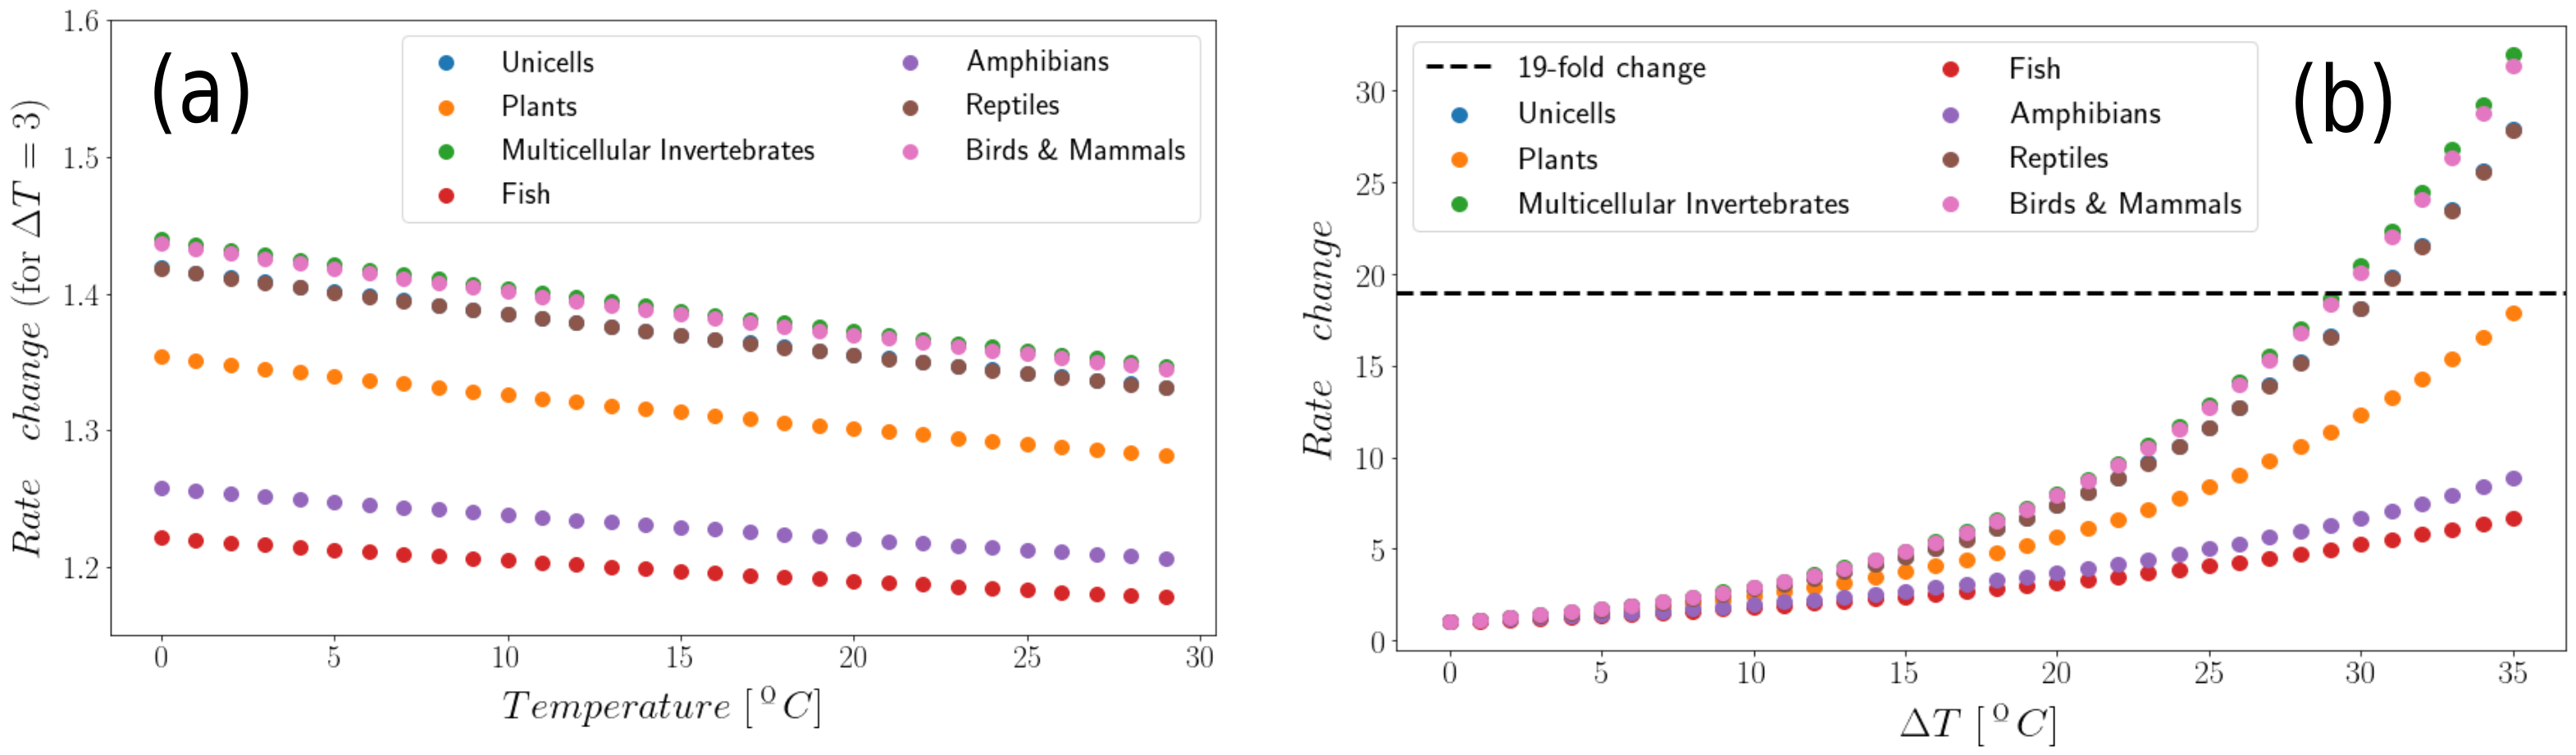
\includegraphics[width=1\textwidth]{Figures/arrhenius.png}
    \caption{Graphical representation of change in the rate (in ordinates)
        for different reference temperatures (in abscissae) for: (a) a
        temperature
        increase of $\SI{3}{\degree C}$; (b)  a temperature increase of
        $\SI{14}{\degree C}$. The black dotted line in (b) corresponds to a
        $19$-fold
        increase in the rate.
    }
    \label{fig:rate_changes}
\end{figure}

%----------------------------------------------------------------------------------------
%	Spatial effects in parasite-induced marine diseases of immobile hosts
%----------------------------------------------------------------------------------------
\chapterimage{nacra2.png}
\chapterspaceabove{6.75cm}
\chapterspacebelow{7.25cm}

\chapter{Spatial effects in parasite-induced marine diseases}
\vspace{3cm}

% \begin{center}
%     \textbf{Àlex Giménez-Romero$^{1}$, Federico Vázquez$^{2,1}$, Cristóbal
%         López$^{1}$, Manuel A. Matías$^{1}$}
% \end{center}

% \vspace{1cm}

% \begin{enumerate}
%     \small
%     \item Instituto de Física Interdisciplinar y Sistemas Complejos, IFISC
%           (CSIC-UIB), Palma de Mallorca 07122, Spain
%     \item Instituto de Cálculo, FCEyN, Universidad de Buenos Aires and CONICET,
%           Buenos Aires, Argentina

% \end{enumerate}

% \vspace{1cm}

\textbf{Published as}

\vspace{0.5cm}

\fullcite{GimenezRomero_2022_RSos_e}

\newpage
\section{Introduction}

Wildlife emergent infectious diseases represent a substantial threat to
ecosystems and the conservation of their biodiversity \cite{Daszak443}. Their
effects can be devastating at the ecological level, causing local extinctions
\cite{Daszak443} and in some cases pushing endemic species to the verge of
extinction, as is the case of \textit{Pinna nobilis}
\cite{Cabanellas2019}; at the economic level, producing losses in agriculture,
livestock and aquaculture \cite{Vurro2010, Tomley2009, Pernet2016}, and impact
human health, as is the case of the COVID-19 pandemic \cite{Salata2020}. For
the past decades, parasites have been continuously emerging \cite{Morens2004,
    Daszak2017}, while globalisation and climate change have contributed to
their
evolution. This has allowed these parasites to enter in new ecological niches
and spread further the diseases they produce \cite{Aguirre2008}. In particular,
marine infectious diseases are recently increasing due to these and other
anthropogenic pressures, like pollution and overfishing \cite{Lafferty2004},
inducing widespread mass mortalities in several species \cite{Eisenlord2016,
    JONES201648, VAZQUEZ2017}.

An important subset of marine organisms affected by infectious diseases are
sessile (i.e. they cannot move), like bivalves, sponges or corals. An
increasing number of outbreaks affecting marine mollusks have been reported,
some of them causing mass mortalities in commercially important bivalves
\cite{Guo2016}. Mainly due to the economic importance of some species (e.g.
oysters), infectious diseases in bivalve populations have been deeply studied
\cite{Petton2021, Pernet2018, McLaughlin2005, powell1999modeling}. Recently,
deterministic compartmental models have been used to describe parasite
transmitted diseases in marine sessile bivalves \cite{BIDEGAIN_2016_2,
    BIDEGAIN_perkinsus, GimenezRomero2021}, showing to be able to accurately
predict disease transmission in some circumstances. The main limitation of
these compartmental models is the assumption of a non-spatial description of
the system under study. This underlying hypothesis assumes that any pair
parasite-host of the system can interact at any time, which is unrealistic in
general. A non-spatial description assumes well mixed populations, which
implies that the mean distance among hosts is smaller than the the typical
distance explored by parasites in their lifetime. This assumption can be quite
realistic in some situations, as it is in \cite{GimenezRomero2021} where the
hosts were kept in tanks with water renovation. However, a non-spatial model is
not expected to yield a good description of spatially extended hosts in a
natural setting.

The key quantity in mathematical epidemiology is the basic reproductive number,
$R_0$, that represents the number of infected individuals generated in one
generation by the appearance of a single infected individual in a fully
susceptible population. Thus, $R_0>1$ ensures the onset of an epidemic, as the
number of infected individuals will grow exponentially	producing a widespread
disease \cite{Anderson1991}. If we first disregard spatial effects and assume a
non-spatial description, $R_0$ can be obtained from standard methods, like the
Next Generation Matrix method \cite{Diekmann2010}, and will only depend on
\textit{intrinsic} characteristics of the pathosystem (host-pathogen system)
under study. However, this basic reproduction number is unable to characterise
the threshold behaviour in many situations, including spatially extended
systems \cite{Cross2007, Li2011, RILEY201568}. In these systems, the
propagation of an epidemic to the entire system needs that a certain spatial
threshold is exceeded \cite{Gilligan2008}. Otherwise the disease will only take
place in suitable localised parts of the system, not being able to propagate to
the total system. Thus, disease spread will be strongly affected by the host
spatial distribution and pathogen mobility, which are not accounted for in
non-spatial models.

In this work we will try to unravel the transmission mechanisms of a
parasite-induced disease affecting immobile hosts in a spatially extended
system. We will approach the problem both theoretically and through numerical
simulation. The numerical study is based on Individual-Based Modelling (IBM), a
method widely used to study ecological systems \cite{Grimm2005}, so that
individuals are treated as discrete entities, space is introduced explicitly
and the dynamics are stochastic. Representative average behaviours can be
obtained by averaging over a sufficient number of realisations, and the
accuracy of the approach can be calibrated by deriving the corresponding
non-spatial limit, that can be confronted with the suitable compartmental model
on which a particular IBM is based. The IBM approach to our problem will allow
to study in depth the relation between pathogen mobility and immobile host
infection. As parasites move randomly over the space, tracking the position of
each parasite at different times turns to be of fundamental importance to
properly capture the stochastic dynamics of infections from parasites to hosts.
Modelling parasites and hosts as individual entities allows to take into
account the spatial and temporal heterogeneity of interactions between them.
This heterogeneity and the level of control in microscopic interactions cannot
be captured by other mathematical approaches such as partial differential
equations. On the other hand, IBMs are mathematically involved, and analytical
treatments are normally cumbersome, while their numerical implementation is
computationally expensive \cite{Breckling1900}.

Here we introduce a spatially-explicit individual-based model to study
parasite-induced marine diseases of immobile hosts. The model is applied  to
the case of diffusing parasites and uniformly distributed hosts. The system
under study is an extension of the compartmental model presented in
\cite{GimenezRomero2021}. As a main result, we find that the occurrence of an
outbreak will depend on the balance between the intrinsic characteristics of
the pathosystem, well represented by the above described non-spatial basic
reproductive number, $R_0$, and features that characterise parasite mobility.
We generalise the basic reproductive number, that we will refer to as
$\tilde{R}_0$, such that it accounts for the number of hosts that get infected
by the appearance of a single infected individual in a fully susceptible
population in a spatially extended system. $\tilde{R}_0$ characterises the
global epidemic and can be written as a product between $R_0$ and a factor
describing parasite mobility. The latter factor is smaller and at most equal to
$1$, which implies that, as it could be expected, it is more difficult to
induce a global outbreak in a spatially extended system (a two dimensional
lattice in our case) that in a well mixed (non-spatial) population.

% The paper is organised as follows: in \cref{sec:model}, we introduce some
% biological considerations for bivalve epidemics, discussed in more detailed in
% Ref. \cite{GimenezRomero2021}, and build the spatially-explicit model. In
% \cref{sec:results}, we present analytical results that are discussed and
% supported by numerical simulations. Specifically, the high mobility limit is
% discussed and connected to the the compartmental model. An approximation for
% the parasite population is discussed. Then, the effect of parasite mobility to
% the epidemic threshold is characterised, deriving an analytical expression for
% the basic reproduction number. Furthermore, the spreading speed of the disease
% and the time-scale to extinction is investigated. Finally, \cref{sec:
%     conclusions} contains some concluding remarks.

\section{The SIRP spatial model} \label{sec:model}

The most important biological features of the system under study are as
follows. First, hosts are immobile, while the disease is transmitted by
parasites produced by infected hosts. There are two mechanisms by which
parasites are cleared from the medium: i) they have a finite life time after
which they die or get inactivated; ii) they get absorbed after they infect a
host and thus are no
longer in the medium and cannot infect other hosts. Recruiting (birth) of hosts
occur at a very slow rate compared to other timescales in the system, and
accordingly it will be considered negligible in the model. Moreover, hosts do
not show long-term immunity, as is typical of invertebrates, like mollusks
\cite{Powell2015}. We also assume that recovery (healing) of infected hosts, if
it occurs, can be neglected. Furthermore, we consider that dead hosts are not a
source of parasites in the medium. See \cref{ch:nacras_I}
\cite{GimenezRomero2021} for a detailed
presentation of the non-spatial SIRP model, including these biological
modelling considerations.

Under these considerations, we introduce an individual-based model with
explicit space characterisation to study the effect of parasite mobility in
disease transmission. We consider a square grid of length $L$ with periodic
boundary conditions and place a single host per site, so that there are $N=L^2$
hosts. The hosts can be in three discrete states: susceptible, $S$; infected,
$I$ and dead (or removed), $R$. Then, we introduce the parasite population as a
new individual with a single state, $P$. Hosts are sessile (i.e. immobile),
while parasites are allowed to move between the lattice sites. As initial
condition we assume that the entire host population is susceptible,
$S(0)=N=L^2$, and that a small initial number of parasites, $P(0)$ is
introduced in the system.

Infection occurs when susceptible hosts filter parasites in their close
proximity. Accordingly, the infection process is implemented between parasites
and susceptible hosts sharing the same lattice site. In particular, susceptible
hosts in contact with a parasite become infected at rate $\beta$. As the
infection event implies the filtering of a parasite by a susceptible host, when
a new infection occurs a parasite of that particular site is removed. Infected
individuals die at rate $\gamma$ and produce parasites at rate $\lambda$, while
parasites die at rate $\mu$. Parasites move randomly between the four
neighbouring lattice sites at rate $\kappa$, which corresponds to a diffusive
motion. \cref{tab:IBM_params} contains the definitions of the variables and
parameters of the model and \cref{fig:IBM} shows a schematic representation of
the dynamics.

\begin{figure}[H]
    \centering
    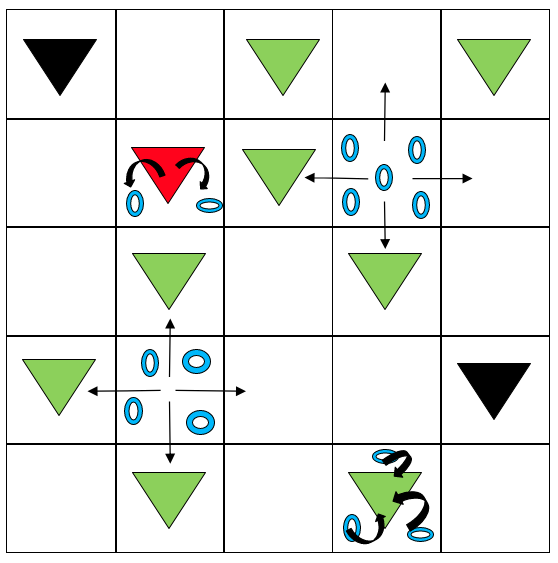
\includegraphics[width=0.6\textwidth]{Figures/IBM.png}
    \caption[Scheme of the individual based SIRP model]{Scheme of the
        individual based model. Green, red and black
        triangles represent susceptible, infected and dead hosts, respectively.
        Blue
        rings represent parasites, which move randomly between cells.
        Susceptible hosts
        get infected by filtering parasites while infected hosts produce them.
        Dead
        hosts do not participate in the dynamics of the system.}
    \label{fig:IBM}
\end{figure}

\begin{table}[H]
    \centering
    \caption[Variables and parameters of the individual based SIRP
        model]{Variables and parameters of the individual based SIRP model.}
    \resizebox{0.8\columnwidth}{!}{
        \begin{tabular}{cl}
            \hline \hline
            \textbf{Variable/Parameter} & \textbf{Definition}
            \\ \hline
            S                           & Susceptible host
            \\
            I                           & Infected host
            \\
            R                           & Dead host
            \\
            P                           & Parasite
            \\
            $\beta$                     & Parasite-host transmission rate
            \\
            $\gamma$                    & Host mortality rate
            \\
            $\lambda$                   & Production rate of parasites by
            infected hosts
            \\
            $\mu$                       & Parasite natural death rate
            \\
            $\kappa$                    & Parasite dispersal rate (mobility)
            \\
            $R_0$                       & Non-spatial basic reproductive number
            \\
            $\tilde{R}_0$               & Spatial basic reproductive number
            \\ \hline \hline
        \end{tabular}
    }
    \label{tab:IBM_params}
\end{table}

Formally, the model is mathematically described by a system of $N$ master
equations for the probabilities of the states in each lattice site $i$.
\cref{eq:scheme} summarises the reactive events. This is
very difficult to manage analytically, so the time evolution of the model is
numerically solved using Gillespie's algorithm \cite{Gillespie1977} (the code
can be found in \cite{CODE_nacras}).
\begin{equation}\label{eq:scheme}
    S+P \stackrel{\beta}{\rightarrow} I + \varnothing \quad I
    \stackrel{\gamma}{\rightarrow} R \quad I \stackrel{\lambda}{\rightarrow}
    I+P
    \quad P \stackrel{\mu}{\rightarrow} \varnothing
\end{equation}

\section{Results}\label{sec:results}
In this section several features of the model are studied, both numerically
(from IBM simulations) and analytically. All numerical results were obtained
for a square lattice of length $L=100$, with $N=S(0)=10^4$ hosts and using a
small initial condition of $P(0)=50$ parasites in the centre site.

\subsection{Non-spatial limit} \label{sec:MFlimit}
An important test of the IBM implementation is to show that, under suitable
circumstances, it converges to the non-spatial model on which the IBM is based.
This occurs in the limit when the parasites move many times before dying or
infecting a susceptible host. In this situation, each parasite typically visits
all the hosts of the system and may infect any of them. This is equivalent to
infecting a random host of the system, which happens with probability $\beta
    S/N$, being $S$ the total number of susceptible hosts in the system.
This corresponds to standard incidence, which represents the most accurate
description of the infection process
(\cref{ch:nacras_I},\cite{GimenezRomero2021}).
An equivalent picture is that parasites will end up uniformly distributed in
the lattice, so that there will be $P/N$ parasites in each lattice site at any
time. One expects to reach these conditions when $\kappa\gg\mu,\beta$, and,
thus the system as a whole can be described by the following system of ordinary
differential equations (ODE's),
\begin{equation}\label{eq:SIRP_MF}
    \begin{aligned}
        \dot{S} & =-\beta P S/N \, ,               \\
        \dot{I} & =\beta P S/N-\gamma I \, ,       \\
        \dot{R} & =\gamma I \, ,                   \\
        \dot{P} & =\lambda I-\beta P S/N-\mu P \ ,
    \end{aligned}
\end{equation}
that is precisely the SIRP non-spatial model \cite{GimenezRomero2021}, where
$S$, $I$, $R$ are the total number of susceptible, infected and recovered hosts
in the system, $P$ the total number of parasites and $N$ is the number of
hosts.

The basic reproduction number, $R_0$, of this non-spatial model is the
dimensionless quantity that yields the number of secondary infections generated
by the appearance of a single infected individual in a completely susceptible
population, also indicating whether the system will exhibit an epidemic
outbreak, $R_0>1$, or not, $R_0<1$.
In our case it can be directly computed as the mean number of parasites
produced by an infected host during its mean lifetime, $\lambda/\gamma$, times
the mean number of susceptible hosts that get infected by parasites during
their mean lifetime, $\beta/(\mu+\beta)$,
\begin{equation}\label{eq:R0_MF}
    R_0=\frac{\lambda}{\gamma}\frac{\beta}{\mu+\beta} \ .
\end{equation}
This result can be corroborated with standard methods such as the Next
Generation Matrix method \cite{Diekmann2010} (see \cite{GimenezRomero2021}),
where $S(0)=N$ has been considered.

Moreover, the model has a conserved quantity $\mathcal{C}$
\cite{GimenezRomero2021} that allows to find an analytical expression for the
final number of dead individuals (\cref{app:Rinf}),
\begin{equation}\label{eq:R_inf}
    R(\infty)=N+\frac{S(0)}{\xi}W_0\parentesi{-\xi\exp(-\frac{\beta}{\mu}C)} \
    ,
\end{equation}
with $\displaystyle\xi=S(0)\frac{\beta\parentesi{\lambda-\gamma}}{\mu\gamma}$
and $\displaystyle C=P_0+\frac{\lambda}{\gamma}\parentesi{S(0)+I(0)}-S(0)$.

The non-spatial limit of the model has been evaluated by comparing realisations
of the stochastic model (in the limit $\kappa\gg\mu,\beta$) with numerical
solutions of the non-spatial ODE system of \cref{eq:SIRP_MF}. Furthermore, the
analytical expression for $R(\infty)$ using the non-spatial model,
\cref{eq:R_inf}, is also compared to the numerical results of the individual
based model. As shown in \cref{fig:MF_limit} (a)-(c), as $\kappa$ is increased
compared to $\mu$ the individual based model approaches the non-spatial one.
\cref{fig:MF_limit}(d) shows how the numerical results for $R(\infty)$ for
different $R_0$ values approach the analytical solution in the non-spatial
limit.

\begin{figure}[H]
    \centering
    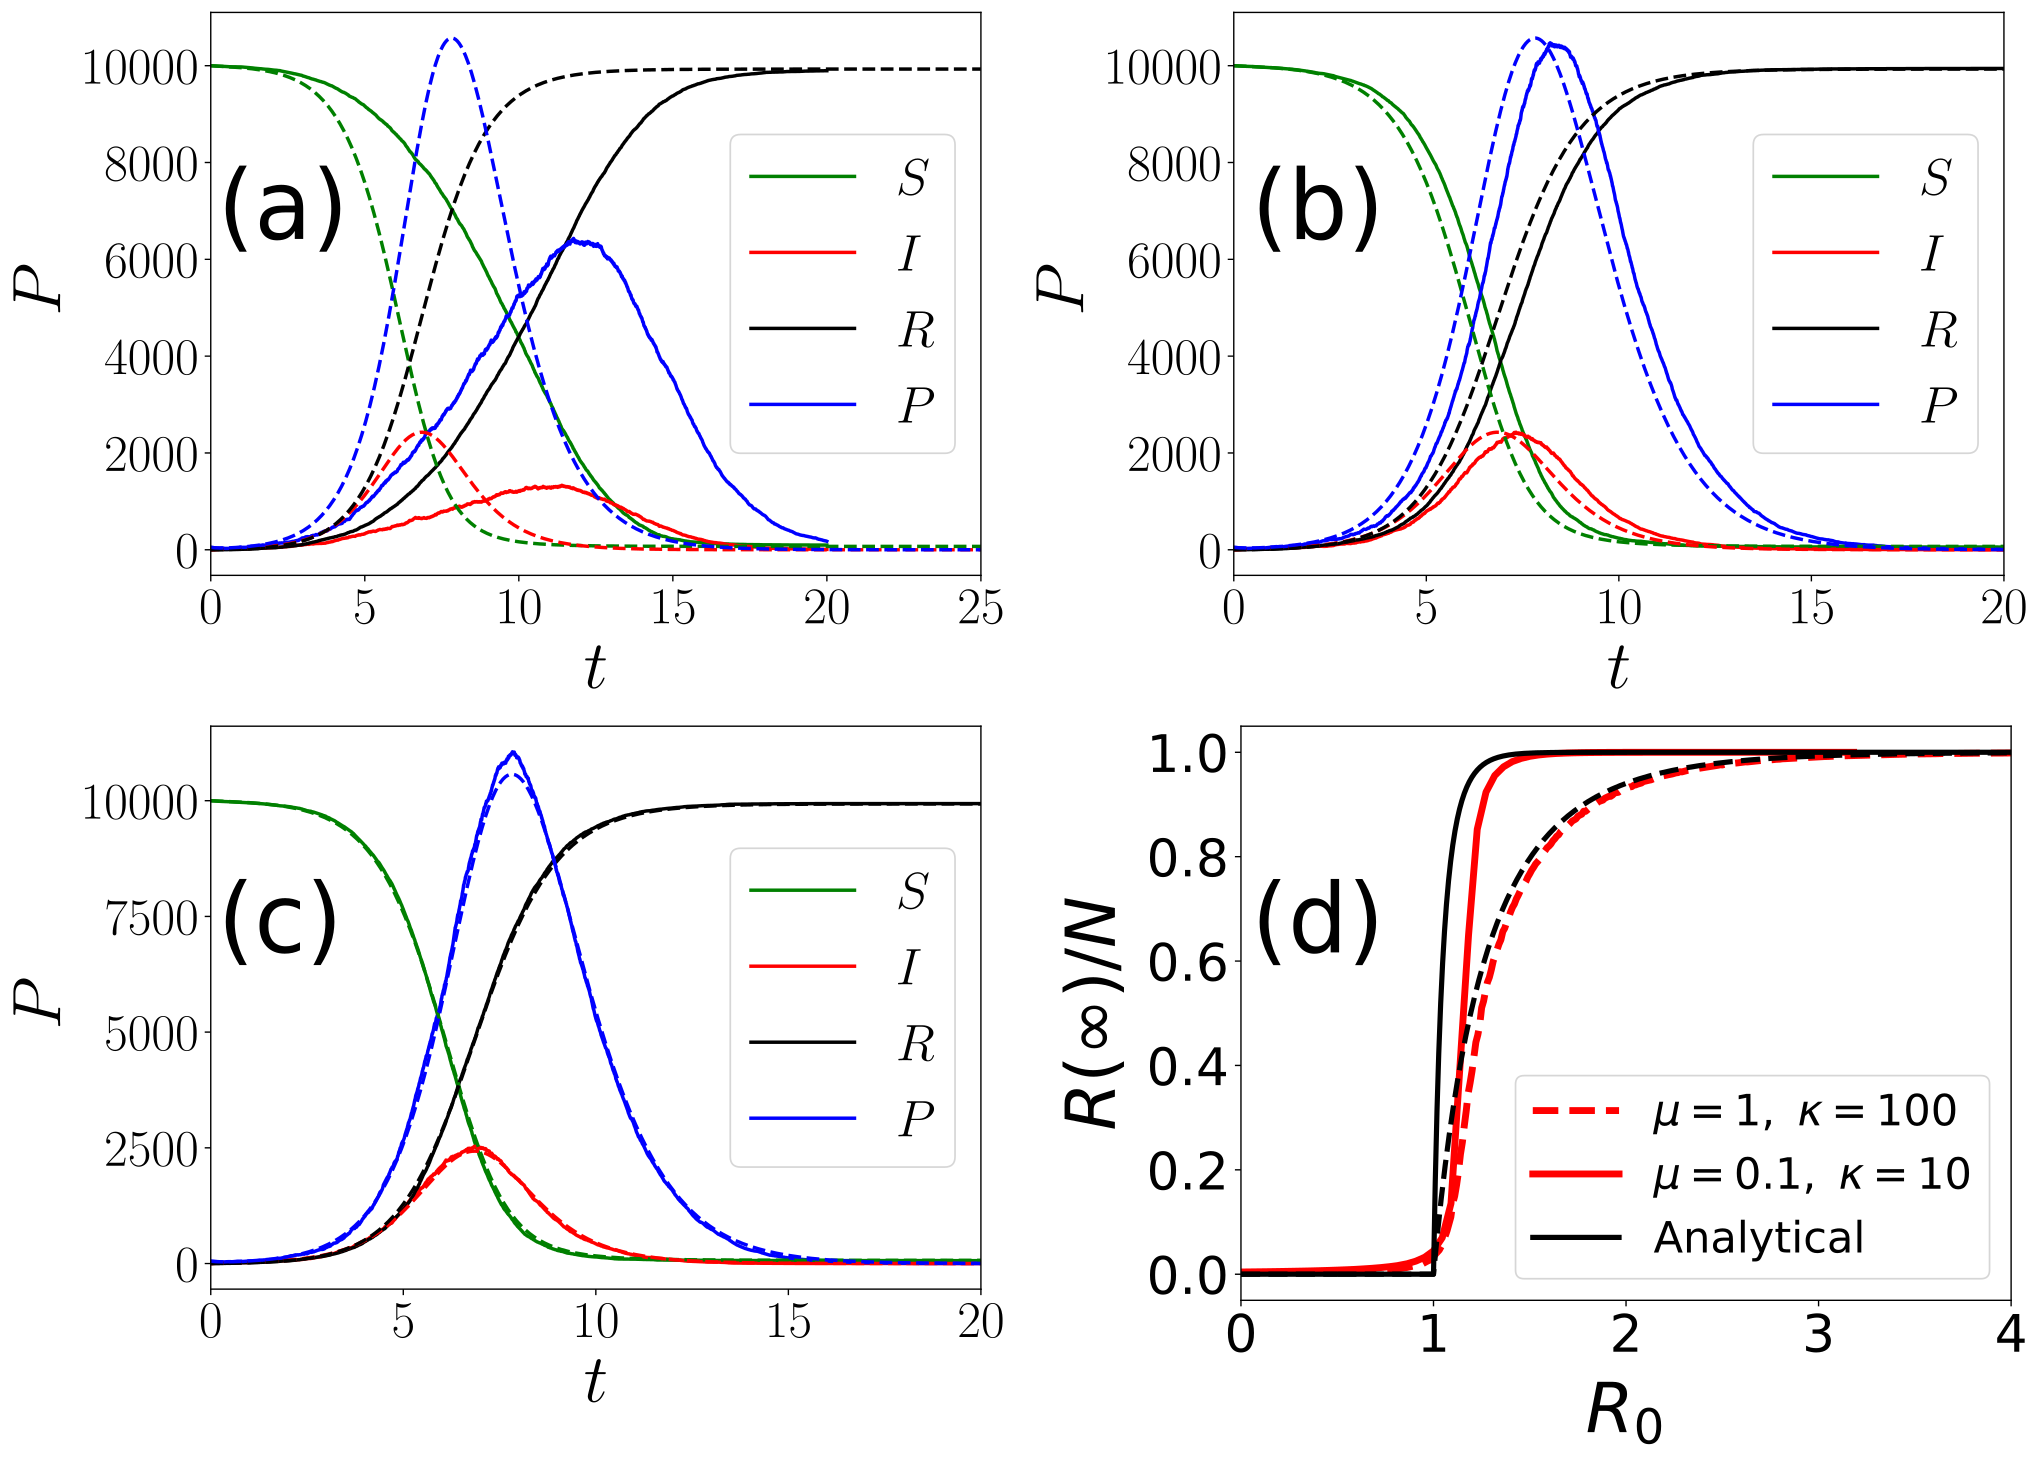
\includegraphics[width=\columnwidth]{Figures/MF_comparison.png}
    \caption[
        Comparison between the non-spatial model and the individual based model
        in the high mobility limit
    ]{Numerical solution of the non-spatial model (\cref{eq:SIRP_MF},
        dashed lines) compared with numerical solutions of the individual based
        model
        (solid lines) approaching the non-spatial limit with fixed
        $\gamma=\mu=\beta=1$
        and $\lambda=6$. (a) $\kappa=10^2$, (b) $\kappa=10^3$, (c)
        $\kappa=10^4$. Panel
        (d) shows the final fraction of dead hosts, $R(\infty)/N$, as function
        of $R_0$
        for $\kappa/(\mu+\kappa)=0.999$ with $\mu=1,0.1$ compared to the
        analytical
        result.}
    \label{fig:MF_limit}
\end{figure}

\subsection{Approximate relation between parasites and infected hosts}

In the limit $\kappa\gg\beta,\mu$ a time-scale approximation can be
performed so that the parasite population dynamics directly relates to that of
the infected hosts. In the non-spatial limit it was already shown in
\cite{GimenezRomero2021} that, if  $\mu\gg\beta,\gamma$ and $\lambda\gg\beta
    P/N$, the total parasite population of the system can be well described
using
the approximation (see \cite{GimenezRomero2021} for a detailed discussion),
\begin{equation}\label{eq:P_approx_II}
    P(t)\approx \frac{\lambda}{\mu} I(t) \ .
\end{equation}

Here we extend the validity of this approximation to spatial systems far
from the non-spatial limit. Consider the local dynamics of the parasite
population on a lattice site $i$. Note that when the host in the site is
susceptible, parasites in this site can either infect the host, die, or move to
another site. All these processes imply that a parasite will disappear from the
current site. Once the host at site $i$ gets infected, infection can no longer
occur whereas parasite production is now possible. If $\kappa$ is small enough
compared to $\lambda$ and $\mu$,  the only competing processes in sites with
infected individuals will be the production of parasites and their natural
death, which can be fairly described by the following rate equation,
\begin{equation}
    \der{P}{t}=\lambda-\mu P \ ,
\end{equation}
which solution is
\begin{equation}\label{eq:P_evol}
    P(t)=\frac{\lambda}{\mu}+\claudator{P(0)-\frac{\lambda}{\mu}}e^{-\mu t}
    \ .
\end{equation}

From \cref{eq:P_evol} one may notice that the stationary value of $P$,
$\lambda/\mu$, is reached in a time proportional to $t_{\textrm{eq}}\propto
    1/\mu$. This derivation allows to find a condition for which
\cref{eq:P_approx_II}
is valid beyond the non-spatial limit. Basically, if the mean dispersal time,
$1/\kappa$, is greater than the equilibrium time, $t_{\textrm{eq}}\propto
    1/\mu$, parasites in sites with infected hosts will reach its stationary
level
before parasites enter or leave the sites. Thus, sites with infected hosts can
be considered as a closed system and the approximation holds. In other words,
if the dispersal rate of parasites is small compared to the parasite
deactivation rate, $\kappa \ll \mu$, the local parasite population of the site
will reach its stationary level $P_i=\lambda/\mu$. It is possible to extend the
result to the entire system: if there are $I(t)$ infected sites in the system
at time $t$ and $\kappa\ll\mu$ is fulfilled, there will be a total parasite
population of $P(t)=(\lambda/\mu) I(t)$, which is equivalent to
\cref{eq:P_approx_II}.

\begin{figure}[H]
    \centering
    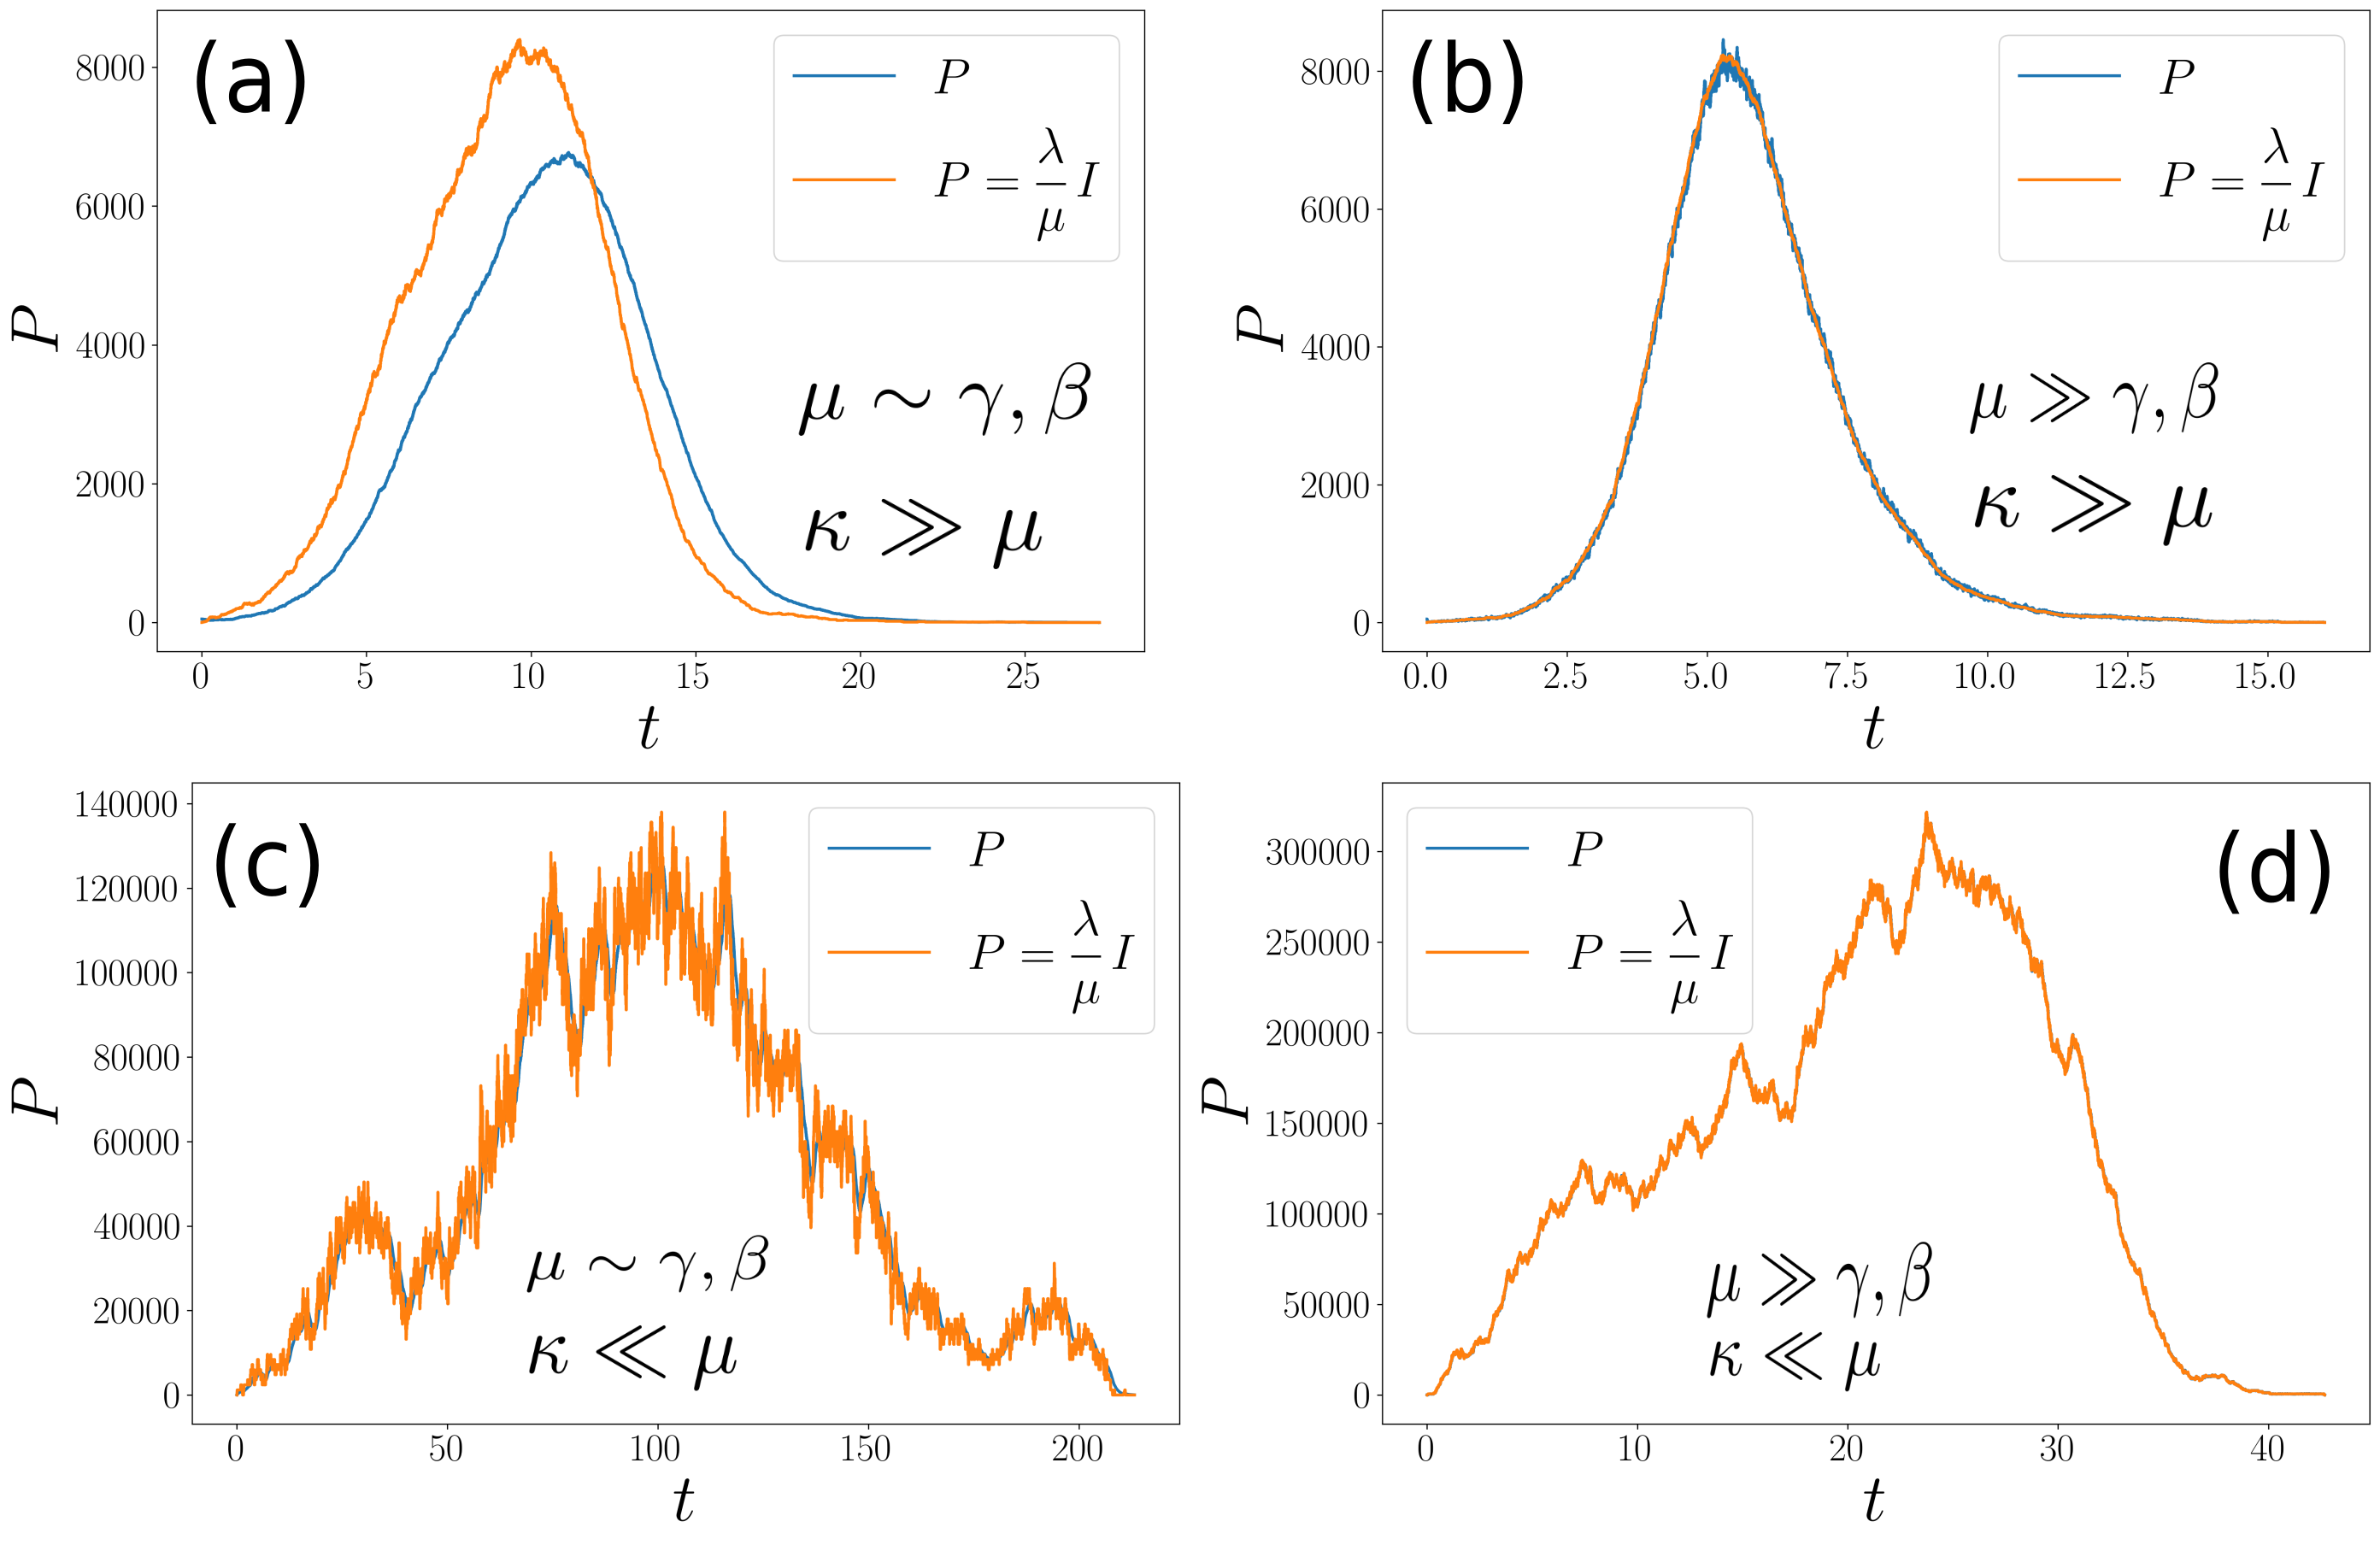
\includegraphics[width=\columnwidth]{Figures/P_approx.png}
    \caption[Validation of the approximate expression for the parasite
        population dynamics]{Numerical verification of the approximate
        expression for the parasite population dynamics, \cref{eq:P_approx_II},
        for different mobility conditions. The simulations were performed
        fixing $\beta=\gamma=1$ for all panels. (a) $\mu=1$ $\kappa=10^2$,
        $\lambda=6.06$, $\kappa/(\mu+\kappa)=0.99$;
        (b) $\mu=100$, $\kappa=10^4$, $\lambda=306$,
        $\kappa/(\mu+\kappa)=0.99$; (c)
        $\mu=1$, $\kappa=0.01$, $\lambda=1200$, $\kappa/(\mu+\kappa)=0.01$; (d)
        $\mu=100$, $\kappa=1$, $\lambda=60600$,  $\kappa/(\mu+\kappa)=0.01$}
    \label{fig:P_approx}
\end{figure}

Thus, for the non-spatial limit ($\kappa\gg\mu$) we have that if
$\mu\gg\beta,\gamma$ \cref{eq:P_approx_II} is valid, while for $\kappa\ll\mu$
the
approximation is also valid regardless of the value of $\beta,\gamma$, as the
nature of the approximation is different. Thus, in general, as $\kappa$
decreases over $\mu$ (the lower the parasite mobility becomes) we expect the
approximation to work better.

The parasite approximation to infected hosts dynamics, \cref{eq:P_approx_II},
is numerically verified for different mobility conditions.
\cref{fig:P_approx}(a)-(b) shows how the approximation improves as $\mu$ grows
over $\beta,\gamma$ (mean errors are $0.18$ and $0.0081$, respectively) in the
non-spatial limit, i.e. $\kappa\gg\mu$, as expected. This result is in perfect
agreement with that found in \cite{GimenezRomero2021}. Then,
\cref{fig:P_approx}(c)-(d) show that the approximation is valid in general when
$\kappa\ll\mu$ but improves anyway when $\mu\gg\beta,\gamma$ (mean errors are
0.04 and 0.0026, respectively). Summarising, we see that the lower the value of
$\kappa$ is with respect to $\mu$ the more valid \cref{eq:P_approx_II} is,
regardless of the value of $\beta,\gamma$, while in the non-spatial limit,
$\kappa\gg\mu$, the condition $\mu\gg\beta,\gamma$ is needed.

\subsection{Spatial threshold}

One of the main questions in epidemiology is to define the conditions under
which an epidemic outbreak occurs, which usually is translated into the
existence of a threshold. In a well mixed (non-spatial) system the basic
reproduction number ($R_0$), that characterises this threshold $R_0=1$, can be
defined exclusively from \textit{intrinsic} parameters of the pathosystem, as
the host-pathogen interaction does not depend on the host spatial structure or
pathogen mobility (see \cref{eq:R0_MF}). In stochastic spatial models this
formulation of $R_0$ breaks down. First of all, in stochastic models, even
above the threshold there is a non-zero probability that the disease is unable
to propagate initially, given by
$P_{\textrm{outbreak}}=1-\parentesi{1/R_0}^{I(0)}$ \cite{Brauer2008}.
Furthermore, the discrete nature of the populations also modifies the estimates
of $R_0$ \cite{KEELING200051}. On the other hand, the introduction of space
changes completely the nature of epidemic outbreaks, modifying the
host-pathogen interactions by means of specific host spatial distributions and
pathogen mobility patterns. Even if the basic reproduction number of the
non-spatial model is above the threshold ($R_0>1$), if parasite mobility is not
large enough, the epidemic will stay locally confined. Thus, one expects that
the threshold at which an epidemic outbreak can propagate to the rest of the
system will depend on the balance between the intrinsic pathosystem parameters
in $R_0$ and parasite mobility, defining a spatial basic reproduction number,
$\tilde{R}_0$.

Having in mind the study in \cref{sec:MFlimit}, we expect that in the high
mobility limit the basic reproduction number is defined by the non-spatial
formula, \cref{eq:R0_MF}. On the other hand, the lower the parasite mobility
is, the more difficult will be for a local outbreak to propagate through the
system. Thus, it is natural to think of an spatial basic reproduction number of
the form $\tilde{R}_0=R_0 f(\kappa)$, where $f(\kappa)$ is an increasing
function of the parasite dispersal rate accounting for parasite mobility
fulfilling $\lim_{\kappa\to\infty}f(\kappa)=1$.

Indeed, some authors recently showed that the spatial basic reproduction
number can be defined as the product between the non-spatial value, $R_0$, and
a factor accounting for spatially-dependent interactions, $f(r)$, in the form
$\tilde{R}_0=R_0f(r)$ \cite{Filipe2003,Filipe2004,Gilligan2021}. However, these
expressions are not analytical \cite{Filipe2003,Filipe2004} or are not directly
related to pathogen mobility \cite{Gilligan2021}. Here we propose a simple
expression for the spatial basic reproduction number regulating the spatial
propagation of the epidemic,
\begin{equation}\label{eq:R_0ibm}
    \tilde{R}_0=\frac{\lambda}{\gamma}\frac{\beta}{\mu+\beta}
    \frac{\kappa}{\mu+\kappa}=R_0\frac{\kappa}{\mu+\kappa}
    \ .
\end{equation}

The derivation of \cref{eq:R_0ibm} accounts for the number of secondary
parasites that are able to produce new infections, or equivalently, the number
of secondary infections produced by an initial infected host. If we consider an
initial infected individual, on average it will produce $\lambda/\gamma$
parasites. Then, these parasites can only move to neighbouring sites or die, so
that the dispersal probability is given by $\kappa/(\mu+\kappa)$. Finally,
considering that parasites do not affect each other trying to infect the same
host, the infection probability is given by $\beta/(\mu+\beta)$. Joining all
terms, we finally obtain \cref{eq:R_0ibm}. This expression is valid when
parasites move only to sites with susceptible individuals and do not try to
infect the same host. Thus, the derived $\tilde{R}_0$ is only an approximation
to the spatial basic reproduction number for the case of an initial
introduction of a small quantity of parasites in a fully susceptible
population.

Note that, as expected, the spatial basic reproduction number is nothing
other than the basic reproduction number of the non-spatial model multiplied by
an increasing function of the parasite mobility, $\kappa/(\mu+\kappa).$ Taking
the limit $\kappa\gg\mu$ in \cref{eq:R_0ibm} (non-spatial limit) the basic
reproduction number of the non-spatial model is recovered. Conversely, in the
limit of very low mobility, the $\kappa/(\mu+\kappa)$ factor is small, and this
has to be compensated with a large value of the non-spatial basic reproduction
number, $R_0$, in order that there is an outbreak, i.e., $\tilde{R}_0>1$.

The spatial threshold, $\tilde{R_0}=1$, given by \cref{eq:R_0ibm}, has been
numerically checked by computing the phase diagram between the absorbing phase
$R(\infty)\approx 0$ (no infection, i.e. disease-free state)  and the active
phase $R(\infty)> 0$ (in which some level of infection has occurred, i.e.
propagation phase) for several values of the parasite mobility and the basic
reproduction number of the non-spatial model, $R_0$ \cref{eq:R0_MF}. The
transition is expected to occur at $\tilde{R}_0=1$, implying from
\cref{eq:R_0ibm} that the dependence of the critical value of $R_0$, say
$R_0^c$, is expected to take the form,
\begin{equation}\label{eq: R_0_crit dependence}
    R_0^c\sim\parentesi{\frac{\kappa}{\mu+\kappa}}^{-1} \ .
\end{equation}
As discussed above, we expect that $\tilde{R}_0=1$ with $\tilde{R}_0$ given
by \cref{eq:R_0ibm} does not represent exactly the spatial threshold, and for
this reason we suggest the more general functional form,
\begin{equation}\label{eq: threshold_corrections}
    R_0^c\sim A\parentesi{\frac{\kappa}{\mu+\kappa}}^{-B} - C\ ,
\end{equation}
to be be fitted to numerical data, where $A=1$, $B=1$ and $C=0$ would imply
a perfect agreement of numerical simulations of the IBM model with
\cref{eq:R_0ibm}.

In order to obtain the phase diagram, we compute the absorbing state of the
model as an average over $1000$ realisations for each value of the mobility and
$R_0$ considered. Then, the critical value $R_0^c$ is computed for each
mobility value as the $R_0$ value for which the fluctuations of the ``order
parameter'' $\displaystyle \chi=\avg{{R(\infty})^2}-\avg{R(\infty)}^2$ are
maximal, as this would be an indication of a transition between the
disease-free and the propagation phases.

\begin{figure}[H]
    \centering
    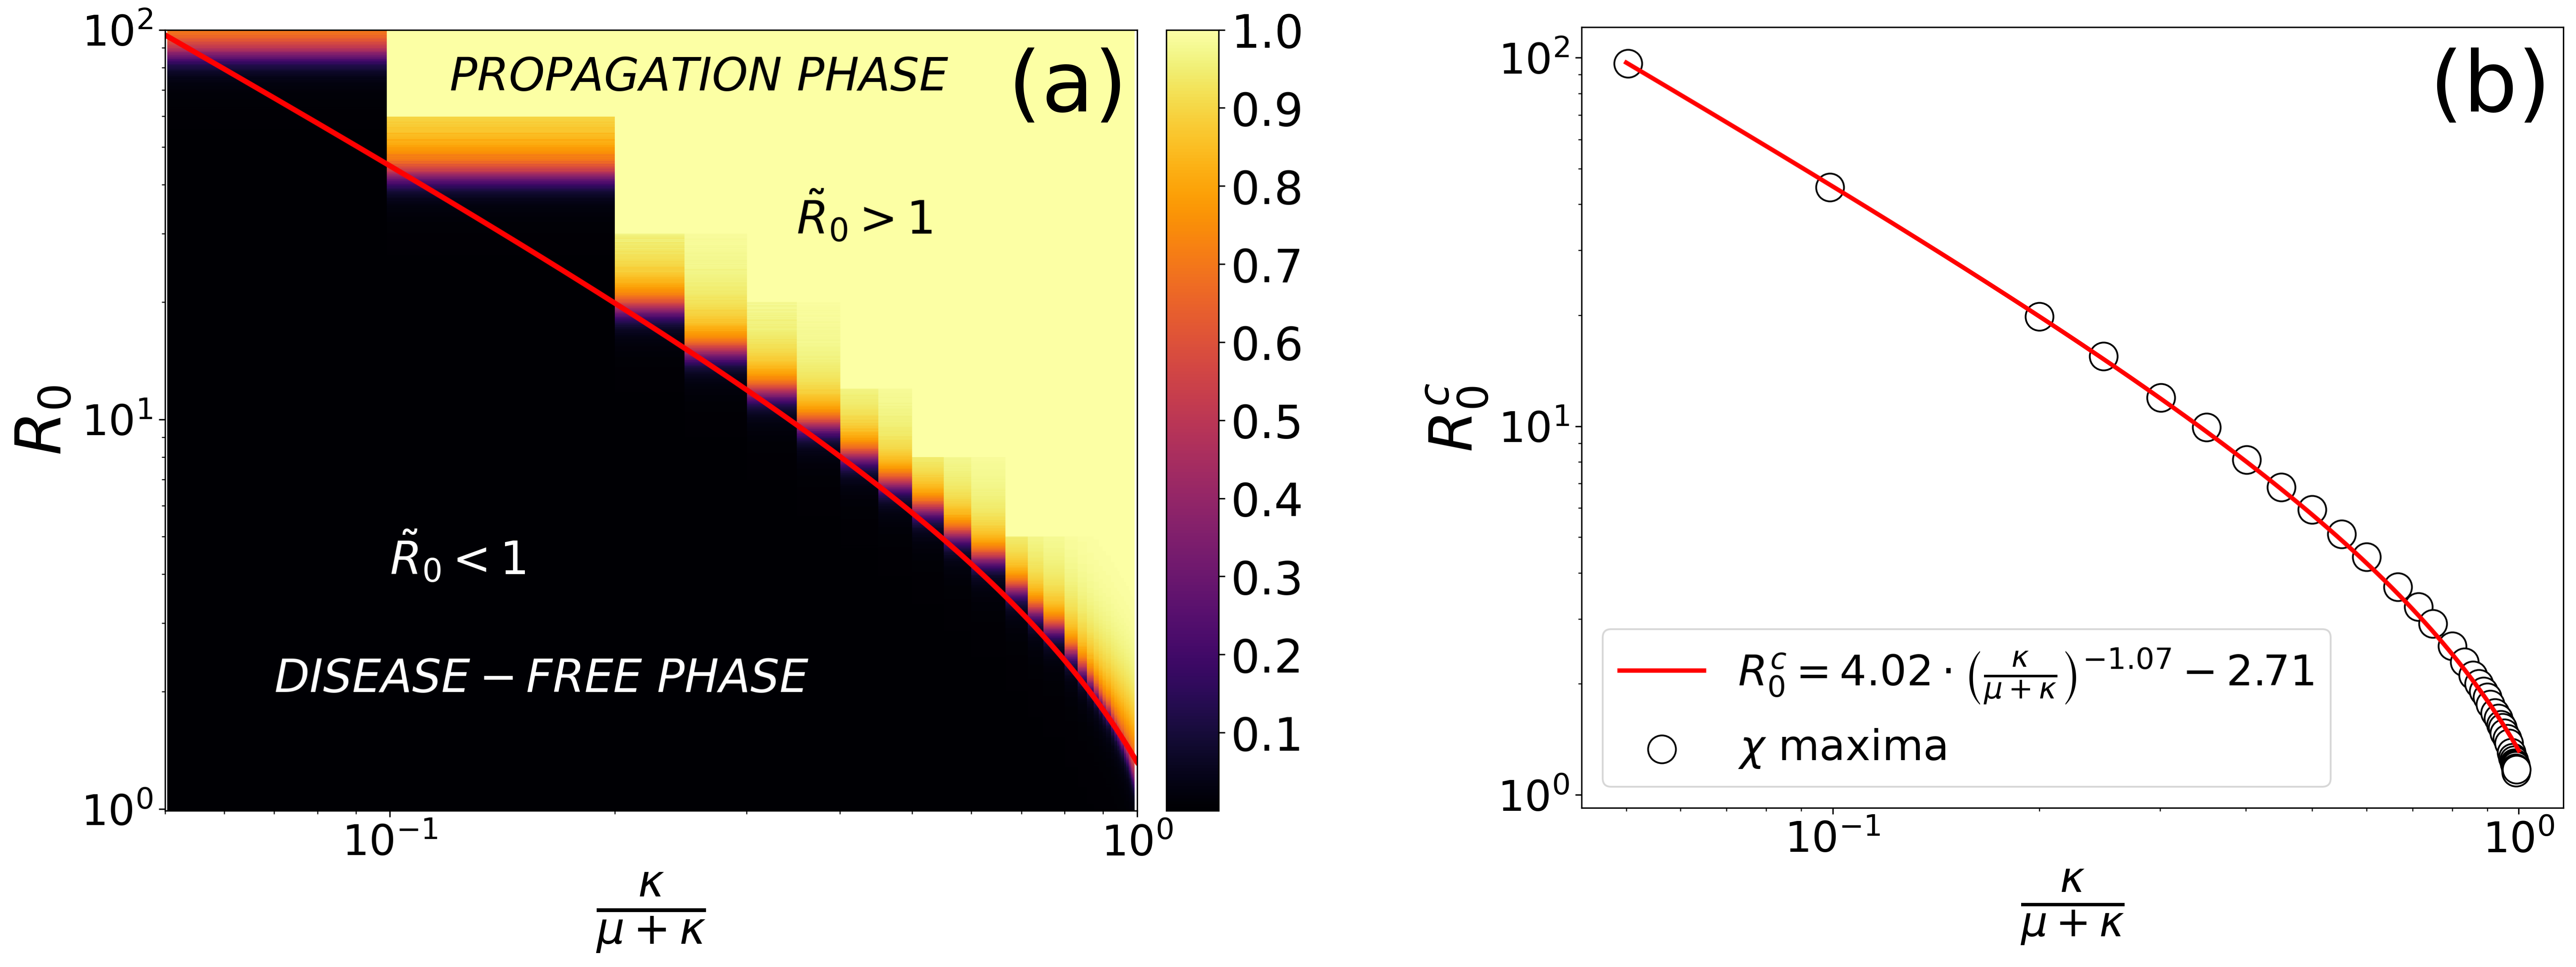
\includegraphics[width=1\textwidth]{Figures/PhaseDiagram.png}
    \caption[
        Phase diagram and fit for the transition between the disease-free and
        propagation phases]{(a) Phase diagram showing the transition between
        the the
        disease-free phase and the propagation phase for several values of the
        parasite
        mobility and $R_0$. The colour code represents the fraction of dead
        individuals
        (i.e. $R/N$) in the final state of the epidemic computed by the average
        over
        1000 realisations. (b) Fit for the transition line following \cref{eq:
            threshold_corrections}, where dots are the maximums of the ``order
        parameter''
        fluctuations, $\chi=\avg{{R(\infty})^2}-\avg{R(\infty)}^2$}
    \label{fig:Phase_diagram}
\end{figure}

\cref{fig:Phase_diagram}(a) shows the numerical results of the computed
transition between the disease-free and propagation phases. The heatmap coding
represents the average value of absorbing state $\avg{R(\infty)}$ for several
values of the mobility factor and $R_0$. As expected, the lower the mobility
factor is, the higher the value of $R_0$ is needed for the disease to invade
the population. \cref{fig:Phase_diagram}(b) shows the fit of \cref{eq:
    threshold_corrections} with less than a $1\%$ of relative error.
Interestingly,
we obtain $B=1.07\approx1$ which validates our expression for the spatial
threshold as a first approximation. However, the values for $A=4.02$ and
$C=2.7$ show a significant deviation from \cref{eq: R_0_crit dependence} and
indicate that the expression \cref{eq:R_0ibm} is  an approximation to the
spatial basic reproduction number, which however seems to contain the right
dependence on $\kappa/(\mu+\kappa)$, and where $A$ could be a geometric factor
for a lattice.

\subsection{Spreading speed of the infected population and time to extinction}

Another relevant epidemiological question is how does an infected
population spread after the onset of an epidemic. In order to obtain this
spreading speed we computed the mean time needed for an infected individual to
reach the boundary of the system. More specifically, for each particular choice
of the model parameters, 1000 simulations were run for several system sizes
ranging from $L=10$ to $L=60$. The computed mean time was found to depend
linearly with the system size, thus allowing to compute the speed from the
slope of this relation. With this procedure, the spreading speed was computed
for several values of the parasite mobility and $R_0$, large enough to ensure
an epidemic outbreak that reached the boundary of the system. In this
situation, the spreading speed is expected to depend linearly with the square
root of the parasite mobility,
\begin{equation}\label{eq:front_vel}
    v\sim\sqrt{\kappa} \ .
\end{equation}

\cref{fig:front_velocity}(a) shows this square root dependence for
different values of the fixed $R_0$. Similarly, the speed was also computed for
several values of the basic reproduction number and a fixed mobility. In this
case, it varies with the square root of the distance to the critical value of
$R_0$, $R_0^c$, as shown by \cref{fig:front_velocity}(b). This is in good
agreement with other mathematically similar models \cite{Bertuzzo2010}.

\begin{figure}[H]
    \centering
    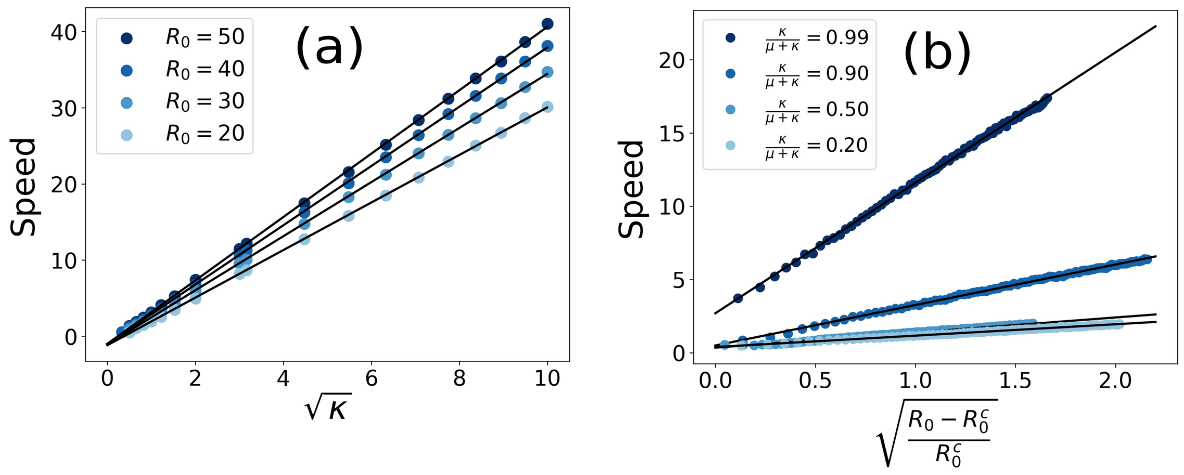
\includegraphics[width=1\textwidth]{Figures/Front_velocity.png}
    \caption[
        Analysis of the spreading speed of the infected population
    ]{(a) Disease spreading speed as function of the square root of
        the parasite mobility for several values of $R_0$. The plot shows a
        remarkable
        agreement with \cref{eq:front_vel}. (b) Disease spreading speed as
        function of
        the square root of the distance to the critical value of $R_0$ for
        several
        values of the parasite mobility.}
    \label{fig:front_velocity}
\end{figure}

The extinction time is defined as the time elapsed from the beginning of
the epidemic until the system reaches its absorbing state, that is, when no
parasites or infected individuals are left. From \cref{eq:front_vel}, we expect
the time to extinction to increase when the parasite mobility is decreased.
Moreover, we expect the extinction time to decrease with the distance to the
epidemic threshold, as we expect to reach faster the absorbing state for larger
values of the spatial basic reproduction number.

In the limiting case where all (or almost all) hosts die, it is clear that
the disease must have spread to the entire system. Thus, in this limit, the
extinction time should be proportional to the inverse of the disease spreading
speed, $t_{\textrm{ext}}\sim 1/v$. Then, in this limit, we can relate the
extinction time with the parasite mobility as follows,
\begin{equation}\label{eq:t_ext}
    t_{\textrm{ext}}\sim\frac{1}{\sqrt{\kappa}} \quad \textrm{for} \quad
    \tilde{R}_0\gg1 \ .
\end{equation}
However, the absorbing state is not always reached after all hosts becoming
infected and \cref{eq:t_ext} is only expected to work far from the epidemic
threshold, when the disease is expected to spread to the entire system.

In \cref{fig:extinction_time}(a) the extinction time is plotted against the
basic reproduction number for some values of the parasite mobility. As
expected, the extinction time increases for lower values of the parasite
mobility. The increasing behaviour before the peak can be understood as the
increasing time needed for the initial perturbations to decay to the
disease-free phase. After the peak, the greater the basic reproduction number
the faster the epidemic will reach its absorbing state with a non-negligible
number of dead individuals. So, with this interpretation, the peaks of the
extinction time should coincide with the epidemic threshold for each value of
the parasite mobility.

\begin{figure}[H]
    \centering
    \includegraphics[width=\textwidth]{Figures/Extinction_time.png}
    \caption[
        Analysis of the extinction time of the epidemic]{(a) Extinction time
        for some values of the parasite mobility.
        (b) Comparison of the critical $R_0$ value computed with
        \cref{eq:R_0ibm}
        compared to the values obtained numerically by computing the maximum of
        the
        extinction time. (c) Scaling of the extinction time with several values
        of the
        parasite mobility. (d) Representation of the square of the extinction
        time as
        function of the inverse of the parasite mobility. The inset shows the
        zone
        where this relation has been computed, showing a good agreement with
        \cref{eq:t_ext}.}
    \label{fig:extinction_time}
\end{figure}

In \cref{fig:extinction_time}(b) we compare the numerical value of $R_0$ at
which the extinction time peaks with the theoretical value of $R_0^c$, computed
with \cref{eq: threshold_corrections}, showing good agreement. Thus, the
dependence of the extinction time with $R_0$ should vanish if plotted against
the distance to $R_0^c$. Furthermore, if the extinction time is normalised
(dividing each line by its maximum), all the lines should collapse near the
transition point. In \cref{fig:extinction_time}(c) the normalised extinction
time is plotted against the distance to the critical value of $R_0$. The
scaling is shown to be valid only near the transition point, as expected.

In the limiting case where the epidemic dies by infecting a large part of
the host population, i.e. for a large enough $R_0$ value, the extinction time
should follow \cref{eq:t_ext}, as previously discussed. In
\cref{fig:extinction_time}(d) we show how the extinction time relates to the
parasite mobility in this limit, following the predicted behaviour.

\section{Conclusions} \label{sec: conclusions}

In this work we have developed a spatially-explicit individual-based model
for parasite-produced marine epidemics of immobile hosts. This study has
allowed us to tackle important questions in marine epidemiology, as how spatial
constraints affect epidemic spreading in filter-feeder populations or how will
the infected population of hosts change in space and time. While addressing the
aforementioned questions, we have shown that there exists a regime of high
parasite mobility where the time progression of both host and parasite
populations can be well described by the non-spatial version of the model (i.e.
the system of ODE's presented in \cite{GimenezRomero2021}). We have also shown
that a fast-slow approximation for the time progression of the parasite
population, already presented in \cite{GimenezRomero2021}, can be extended for
spatial systems. Interestingly, the conditions under which this approximation
is valid  are less restrictive than in the non-spatial case, and regimes in
which this approximation is valid for low mobility and comparable time scales
are reported in this contribution.

We have derived an approximate analytical expression of the
\textit{spatial} basic reproduction number, that allows to predict the onset of
a global epidemic in a spatial model. The obtained expression explicitly shows
a trade-off between the intrinsic pathosystem dynamics (i.e. $R_0$) and a
factor accounting for parasite mobility. Moreover, the spatial threshold
defined by $\tilde{R}_0=1$ separates the final state of the system in two
different phases, namely a disease-free phase and a propagation phase. In the
propagation phase, any initial condition of infected individuals or parasites
will propagate throughout the system, causing a proper outbreak. On the other
hand, in the disease-free phase the conditions are not sufficient for a local
introduction of parasites or infected individuals to spread through the system.
The effect of the parasite mobility in the spatial basic reproduction number is
clear, the more parasites move the more infections they cause.

The spatiotemporal behaviour of the system has been investigated in the
propagation phase. First, we showed that the infected population spreads
through the space with a speed directly proportional to the square root of the
diffusion coefficient of parasites, showing good agreement between the derived
analytical expression and numerical simulations. The time to extinction has
been also studied by means of numerical simulations, showing that, if the
system is far above enough of the spatial threshold, the time to extinction can
be analytically computed, in good agreement with simulations. We obtained that
larger values of the parasite mobility yield more severe epidemics in which
there are more infections and the extinction is faster.

To summarise, in the present work we have introduced and analysed and
Individual-Based approach to epidemic transmission in spatially extended
systems of immobile hosts. The infection mechanism is due to mobile parasites,
that are in turn produced by infected hosts. The study allows to answer some
biologically relevant questions, like predicting the occurrence of a global
epidemic outbreak or its velocity of expansion through the system. Thus, the
analytical and computational results of the model shed light on the underlying
mechanisms underpinning the emergence of a global epidemic outbreak and its
spatial progression. This work provides a first step into the spatial-explicit
individual-based modelling of marine epidemics of immobile hosts.

Although this work has considered the case of a spatially homogeneous
distribution of hosts, we plan to extend the study to more general cases,
discussing the effect of inhomogeneous spatial host distributions. Furthermore,
other biological relevant effects could be added to the model to enhance the
description of different epidemics, e.g. infected individuals could still
filter parasites or parasite-load dependent infection process. The model could
also describe epidemics on other immobile species such as filter feeders like
sponges or other bivalves, corals, intertidal communities or starfishes
provided that the necessary modifications in the model are properly included.
Stochastic spatially-explicit descriptions like the one presented here could be
also extended to the study of epidemics of other immobile hosts, like
vector-borne diseases of plants. However, this would imply a quite different
model to describe the different epidemic compartments of the vectors and also
their ecological features. We hope these studies can be useful in conservation
plans or ecosystem management and could serve as a basis for more sophisticated
models.

%----------------------------------------------------------------------------------------
%	PART III: Towards more realistic models for Xylella fastidiosa spread
%----------------------------------------------------------------------------------------
{
	\hypersetup{hidelinks}
	\part{Vector-borne plant diseases}\label{part:VBD}
}
\thispagestyle{empty}

\begin{center}
    \textbf{\Large Summary}
\end{center}

Vector-borne plant diseases are a significant threat to agriculture, with the
potential to cause widespread epidemics, food shortages, and economic losses.
In particular, the bacterium \textit{Xylella fastidiosa} has emerged as a major
concern for the agricultural sector, affecting a wide range of crops worldwide.
Despite extensive research, many aspects of the dynamics of vector-borne plant
diseases remain poorly understood. For instance, the dynamics of the vector
population, which play a crucial role in disease transmission, is often
neglected in existing models. This is particularly important for
\textit{Xylella fastidiosa} diseases, where the vector population exhibits
complex non-stationary dynamics that are not captured by traditional
models. In this part, we focus on the modeling of vector-borne plant disease
in which the vector population follows complex non-stationary dynamics. We
develop a theoretical framework for modeling vector-borne diseases with
growing or decaying vector populations. We show that traditional methods to
predict the onset of an epidemic do not apply in this context, propose new
approaches, and demonstrate that these dynamics can have a significant
effect on the temporal patterns of disease spread, leading to unexpected
outcomes that are not captured by traditional models. This work has
enabled the construction of a model for \textit{Xylella fastidiosa} diseases
that explicitly incorporates the complex dynamics of the vector population. We
validate the model using empirical data, demonstrating its predictive power and
practical utility. Finally, we provide insights into the design of effective
control strategies that take into account the dynamics of the vector
population. We address current gaps in our understanding of how non-stationary
vector dynamics influence disease spread and severity, offering new insights
into the management and control of these impactful plant diseases.

\vspace{1cm}

\begin{objectiveslist}
    \item To develop a theoretical framework for modeling vector-borne
    diseases with non-stationary and non-periodic vector populations.

    \item To investigate the impact of this type of vector dynamics on
    disease spread and severity.

    \item To construct a model for \textit{Xylella fastidiosa} diseases that
    captures the dynamics of the vector population observed in the field.

    \item To validate the developed model using empirical data.

\end{objectiveslist}

% \vspace{1cm}

% \begin{contributionslist}
%     \item We introduce a theoretical framework for modelling vector-borne
%     diseases with non-stationary and non-periodic vector populations.

%     \item We show that traditional methods to predict the onset of an epidemic
%     do not apply in this context and propose new approaches to address this
%     challenge.

%     \item We develop a model for \textit{Xylella fastidiosa} diseases that
%     explicitly incorporates the dynamics of the vector population.

%     \item We validate the model using empirical data, demonstrating its
%     predictive power and practical utility.

%     \item We provide insights into the management and control of
%     \textit{Xylella fastidiosa} diseases based on the model predictions.
% \end{contributionslist}

%----------------------------------------------------------------------------------------
%	Vector-borne diseases with non-stationary vector populations: the case
%   of growing and decaying populations
%----------------------------------------------------------------------------------------
\chapterimage{olivar_tramuntana.jpg}
\chapterspaceabove{6.75cm}
\chapterspacebelow{7.25cm}

\chapter{Non-stationary vector populations}
\vspace{1cm}

\textbf{Àlex Giménez-Romero$^{1}$, Rosa Flaquer-Galmés$^{1,2}$, Manuel A.
    Matías$^{1}$}

\vspace{1cm}

\begin{enumerate}
    \small
    \item Instituto de Física Interdisciplinar y Sistemas Complejos, IFISC
          (CSIC-UIB), Palma de Mallorca 07122, Spain
    \item Grup de Física Estadística, Departament de Física. Facultat de
          Ciències, Universitat Autònoma de Barcelona, 08193 Bellaterra
          (Barcelona),
          Spain

\end{enumerate}

\vspace{1cm}

\textbf{Published as}

\vspace{0.5cm}

\fullcite{GimenezRomero2022_PRE}

\newpage
\section{Introduction}\label{sec:intro}

Vector-borne diseases are caused by infectious agents transmitted by living
organisms, called vectors,  frequently insects. These diseases represent a
significant threat to global human health \cite{Athni_2020}, causing diseases
such as malaria, dengue, yellow fever, Zika, trypanosomiasis and leishmaniasis
\cite{SCHUMACHER2018352}. Vector-borne human diseases are responsible of more
than 17\% of all human infectious diseases, causing millions of cases and more
than $700\,000$ deaths annually \cite{WHO}. Moreover, crop production and farm
profitability are also affected by bacterial \cite{HUANG20201379} and virus
\cite{Bragard2013} vector-borne diseases. Some examples are the Pierce's
Disease of grapevines, that has resulted in an annual cost of approximately
\$100 million in California alone \cite{tumber2014pierce}, the olive quick
decline syndrome, which could cause about 5 and 17 billion US\$ of losses in
Italy and Spain over the next 50 years in the absence of disease control
measures \cite{Schneider2020} and the multiple diseases caused by viruses
\cite{Rybicki2015}, with diseases like the tobacco mosaic, tomato spotted
wilt, etc., transmitted by aphids and other vectors.

Compartmental deterministic models, e.g. the well known SIR model
\cite{McKendrick}, have been widely used in the modeling of vector-borne
diseases after the seminal work of Ross and Macdonald \cite{Macdonald1957},
that opened the way to controlling malaria outbreaks by acting on the vectors
of the disease (the \textit{Anopheles} mosquito). These models consider that
both host and vector populations can be divided into different compartments
describing different states of the individuals, such as susceptible, infected
or removed (recovered or dead) \cite{Brauer2008}, and the time-evolution of
these compartments is expressed as a system of ordinary differential equations,
defining a dynamical system. Compartmental models provide a mean-field
description, that imply well-mixed (in practice spatially homogeneous)
populations. The well mixed approximation will be valid whenever the mean
distance among hosts is smaller than the mixing length of vectors before they
die. In the case of vector-borne diseases it is also equivalent to every vector
effectively interacting with all the hosts and every host with all the vectors.
A mean-field description is not always valid in spatially extended systems, but
still it is often the first step before writing a spatially explicit
description.

The most relevant piece of information about a disease is whether an
epidemic outbreak will take place or not. The \textit{basic reproduction
    number}, $R_0$, measures the number of secondary infections caused by an
initial infected individual in a fully susceptible population, defining the
epidemic threshold \cite{Anderson1991, VandenDriessche2017}, that determines
the emergence (or not) of an outbreak. If $R_0>1$ an epidemic outbreak will
occur, while there will be no outbreak otherwise. The standard way of computing
$R_0$ in deterministic compartmental models is based on the existence of an
initial disease-free (pre-pandemic) equilibrium, represented by the absence of
infected hosts and vectors \cite{Lauko2006, Kamgang2008}. Some standard
methods based on the linear stability condition of this equilibrium have been
developed to allow the direct computation of $R_0$, such as the Next-Generation
Matrix (NGM) method \cite{Diekmann2010}.

In the case of vector-borne diseases, some models assume that populations
(both hosts and vectors) do not change with time (see e.g.
\cite{Macdonald1957, Brauer2016, VandenBosch2017}), thus assuming equal birth
and death rates. This guarantees the existence of a disease-free equilibrium
and the proper use of standard methods to determine $R_0$. However, this
assumption could be far from reality in several pathosystems. For example, the
interaction between temperature, precipitation variations and other factors may
lead to strong variations in the vector population
\cite{garms1979studies,Rocklov2020}, implying that the pre-pandemic state may
not be an equilibrium state and that standard methods cannot be applied.

Compartmental models of vector-borne diseases have another feature that may
hinder their practical applicability. Namely the fact that these models have
many compartments, that describe the different states of both hosts and
vectors, and as a consequence a relatively large number of parameters. This may
lead to an issue known as \textit{parameter identifiability and uncertainty}
\cite{Chowel2017}, depending on the available data, that is more likely to be
found in models with many compartments and parameters \cite{Roosa2019}.
Usually, parameter estimation procedures are needed to connect the models with
disease data, mainly using incidence or prevalence over time in the host
population. Unfortunately, under many circumstances the underlying model
parameters are unidentifiable, so that many different sets of parameter values
produce the same model fit \cite{Kao2018}. Moreover, these parameters can be
really difficult to determine from the available experimental data.
Nevertheless, in some cases, mathematical manipulations can be performed to
reduce the model complexity using exact or approximate relations
\cite{GimenezRomero2021}. In such cases, the number of parameters of the models
can
be usually reduced in terms of new parameters defined as combinations of some
of the original parameters.

The plan of this paper is as follows. In \cref{sec:model} we develop a
compartmental model of vector-borne transmitted diseases with constant, but
different, birth and death rates for the vectors, that we will use to describe
the case of growing and decaying vector populations. For simplicity, the model
assumes that there is no host to host direct transmission and that the
development of the disease is faster than host recruitment, which is also a
realistic assumption in  many cases, like plant diseases. \cref{sec:results}
contains the main results of the study. In particular, we show that the
asymptotic approach fails to estimate the $R_0$ of the model, overlooking
outbreaks if some conditions are fulfilled. Here, we provide an alternative
method to compute $R_0$ based on the average number of secondary host
infections produced by a primary infected host in one generation. It turns out
that the validity of the  asymptotic approach depends, among other things, on
some time-scales of the model. Furthermore, we discuss and apply some
approximations that allow to reduce the model in favor of simpler ones, with
both fewer compartments and fewer parameters. In particular, we show that if
some of the parameters fulfill certain conditions, it is possible to reduce the
original model with five compartments and four parameters to a SIR model, with
three compartments and two parameters. It is expected that model reductions
like this one significantly help in solving possible problems of parameter
unidentifiability that plague these models. It is interesting to note that a
model in which hosts do not interact directly, but only through vectors, in a
certain limit becomes described as if hosts would infect directly one to each
other, what is assumed in some studies without suitable confirmation. Finally,
the main concluding remarks of the study are presented in
\cref{sec:conclusions}.

\section{The model}\label{sec:model}

The compartment model for vector-borne diseases that we will use to
illustrate the points to be discussed in this study consists of $5$
compartments, $3$ of which describe the host population (susceptible, $S_H$,
infected, $I_H$, and removed, $R_H$), while the other $2$ describe the vector
population (susceptible $S_V$ and infected vectors, $I_V$). Thus, we consider
that the pathogen affects only the hosts and do not consider exposed
compartments. In addition, no direct host to host or vertical (or mother to
offspring for vectors) transmission is assumed. The model could be also
generalized to include an exposed host compartment and the above mentioned
transmission modes, which would hinder the theoretical analysis without
altering the qualitative conclusions of the study. Finally, for the host
population we consider neither recruitment nor natural death and then the total
host population, $N_H$, is constant, $N_H=S_H+I_H+R_H$. Finally, we assume that
infected hosts do not have a mechanisms to combat the disease and become
susceptible again. These assumptions are reasonable in the case of many
phytopathologies.

The model is defined according to the following processes,
\begin{equation}\label{eq:scheme_infection}
    \begin{aligned}
         & S_H+I_V \stackrel{\beta}{\rightarrow} I_H + I_V \quad I_H
        \stackrel{\gamma}{\rightarrow} R_H                           \\
         & S_V+I_H \stackrel{\alpha}{\rightarrow} I_V+I_H \quad S_V
        \stackrel{\mu}{\rightarrow} \varnothing \quad I_V
        \stackrel{\mu}{\rightarrow}
        \varnothing
        \ ,
    \end{aligned}
\end{equation}
which are graphically described in \cref{fig:model_diagram}, being the
birth of new susceptible vectors described as a source term.
Thus, the host-vector compartmental model is written as,
\begin{equation}\label{eq:SIR_v}
    \begin{aligned}
        \dot{S}_H & =-\beta S_H I_v / N_H                     \\
        \dot{I}_H & =\beta S_H I_v / N_H - \gamma I_H         \\
        \dot{R}_H & =\gamma I_H                               \\
        \dot{S}_v & = \delta C-\alpha S_v I_H / N_H - \mu S_v \\
        \dot{I}_v & =\alpha S_v I_H / N_H - \mu I_v \ ,
    \end{aligned}
\end{equation}
where the crossed nonlinear terms, $S_x I_y$ are written divided by the
total host population, $N_H$, what corresponds to the so called standard
incidence, which differs of the purely bilinear form known as mass action
incidence \cite{MartchevaBook}.

The model describes infection of susceptible hosts, $S_H$, at a rate
$\beta$ through their interaction with infected vectors, $I_v$, while
susceptible vectors, $S_v$, are infected at a rate $\alpha$ through their
interaction with infected hosts $I_H$. Infected hosts exit the infected
compartment at rate $\gamma$, while infected vectors stay infected the rest of
their lifetime, as we consider that the pathogen does not affect them, as it is
customary. Vectors die naturally (or disappear from the population by some
mechanism) at rate $\mu$ and are born (appear) at a constant rate $\delta$
being susceptible. The constant term $C$ sets the scale of the stationary value
of the vector population. \cref{fig:model_diagram} shows an schematic
representation of the model and we refer to \cite{Brauer2016} for a similar
model of vector-borne diseases. However, the model in \cite{Brauer2016}
includes exposed compartments and direct host to host transmission, but assumes
that the birth and death rate of vectors are identical, and thus, the
population does not change with time and stays as fixed by the initial
condition.
\begin{figure}[H]
    \centering
    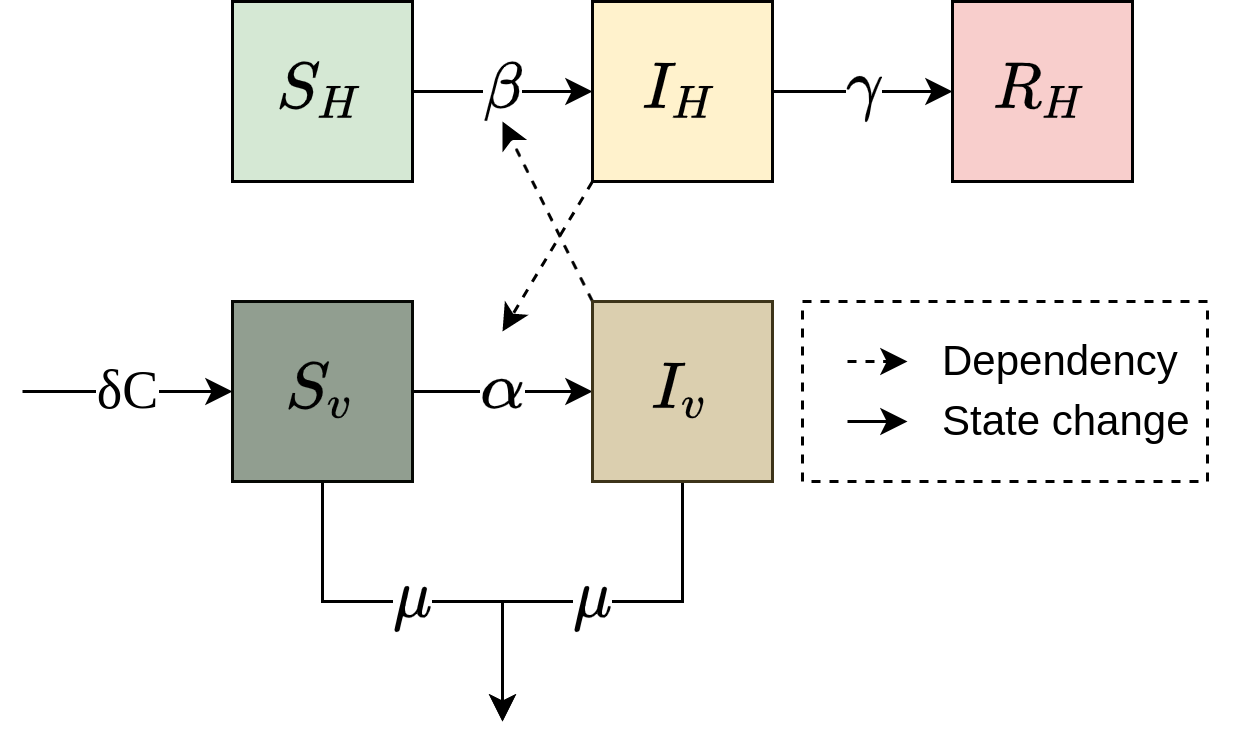
\includegraphics[width=0.9\textwidth]{Figures/Diagram.png}
    \caption{Schematic representation of the model n \cref{eq:SIR_v}. Boxes
        are the compartments in which the population is divided, solid arrows
        represent
        changes in state (so transitions between compartments), and dashed
        arrows
        depict the crossed interaction between hosts and vectors.}
    \label{fig:model_diagram}
\end{figure}

\subsection{Preliminary analysis of the model} \label{sec:Prelimanalysis}

From \cref{eq:SIR_v} it is straightforward to verify that the population of
hosts remains constant over time, $N_H=S_H+I_H+R_H$, while the vector
population fulfills,
\begin{equation}\label{eq:dif_eq_Nv}
    \dot{N}_v=\dot{S}_v+\dot{I}_v=-\mu\parentesi{S_v+I_v}+\delta C=-\mu N_v
    + \delta C \ ,
\end{equation}
with solution,
\begin{equation}\label{eq:Nv_t}
    N_v(t)=\frac{\delta}{\mu}C +
    \parentesi{N_v(0)-\frac{\delta}{\mu}C}e^{-\mu t} \ .
\end{equation}
From \cref{eq:Nv_t} one can write the stationary value for the vector
population, $N_v^*$,
\begin{equation}
    N_v^*=\lim_{t\to\infty}N_v(t)=\frac{\delta}{\mu}C \ .
    \label{eq:asympt}
\end{equation}
Thus, if the initial population of vectors is below (above) the stationary
value, the vector population will grow (decrease) until it reaches the
stationary value. On the other hand, if $N_v(0)=N_v^*=\delta C/\mu$ the initial
population of vectors is already at the stationary state. The initial condition
for the vector population can be written in terms of its stationary value
\cref{eq:asympt}, $N_v(0)=fN_v^*$, where both $f<1$ and $f>1$ are possible, so
that one gets,
\begin{equation}\label{eq:Nv_t_fraction}
    N_v(t)=N_v^*\claudator{1+\parentesi{f-1}e^{-\mu t})} \ .
\end{equation}

We note that vector-borne disease models that assume constant vector
populations (e.g.\cite{Brauer2016}) can be recovered by setting $\delta=\mu$
and $C=N_v(0)$, so that any initial condition for the vector population is
stationary, i.e. $\dot{N}_v=0$ in \cref{eq:dif_eq_Nv} and $N_v(t)=N_v(0)$. We
note that our model describes populations with an asymptotic stationary vector
population and cannot describe periodic vector populations.

\section{Results} \label{sec:results}

%\subsection{The basic reproduction number for stationary vector populations}
\subsection{Epidemic threshold and disease dynamics}
\label{sec:R0statvp}

\begin{figure*}[t!]
    \centering
    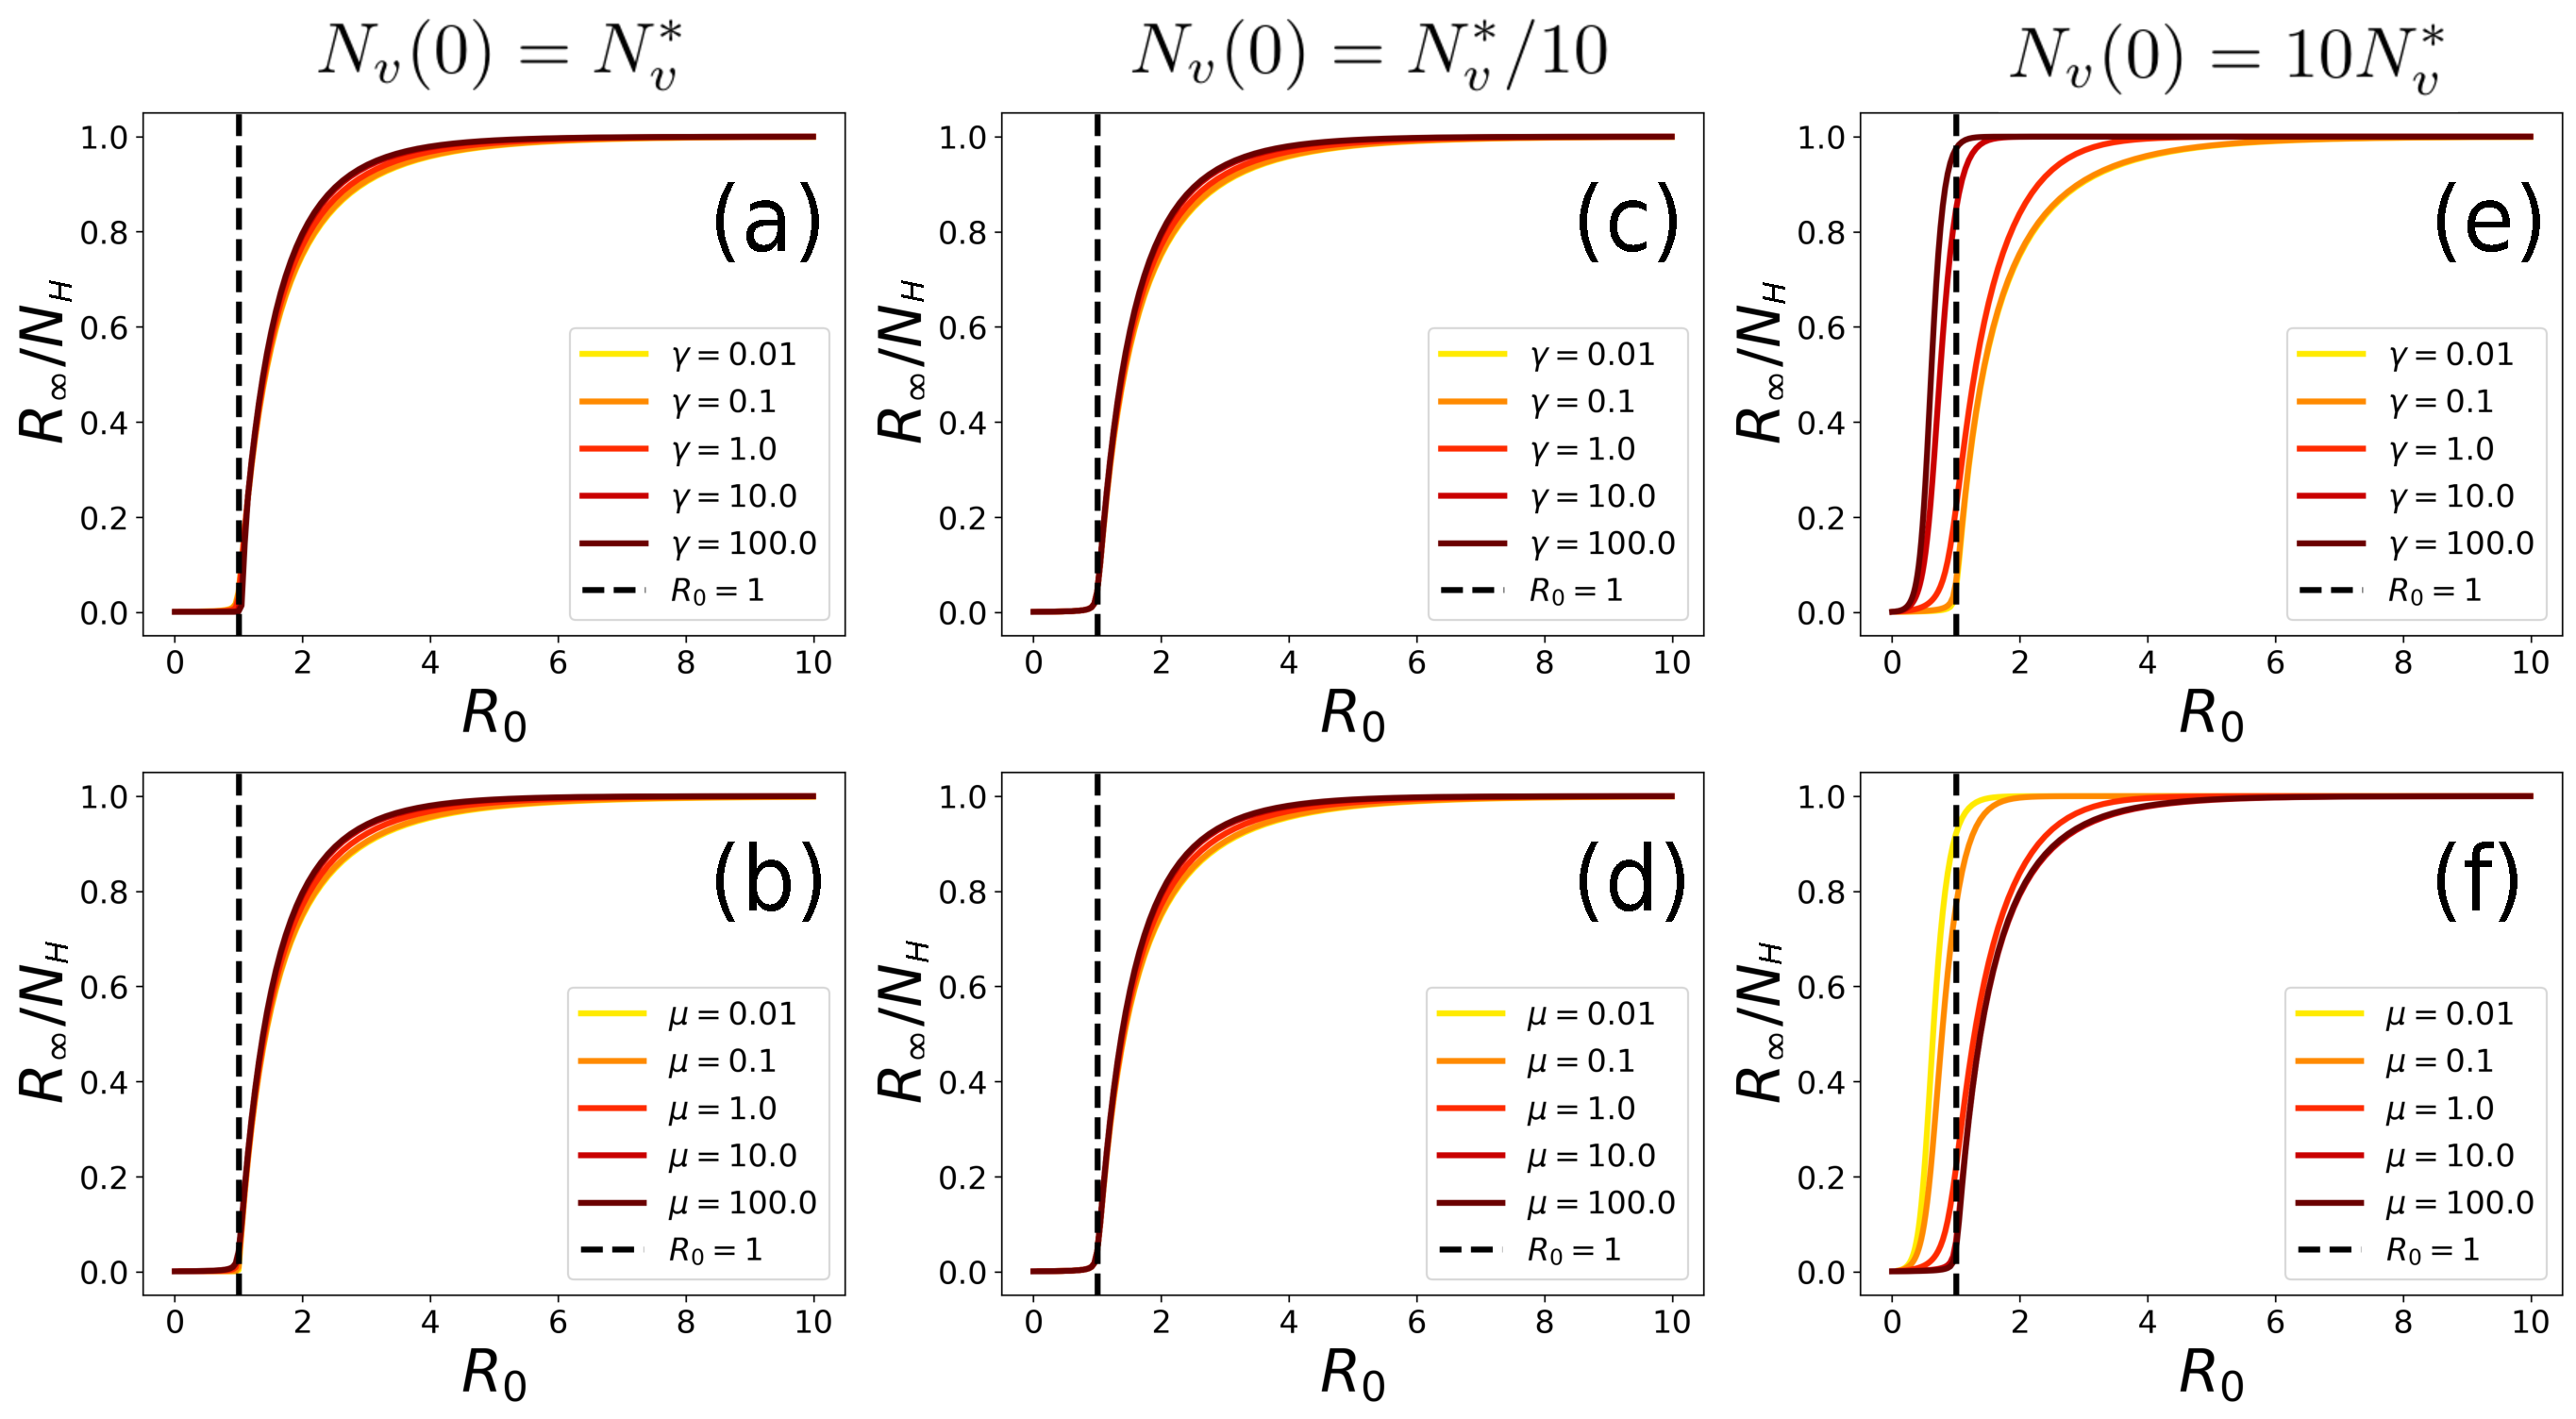
\includegraphics[width=\textwidth]{Figures/R0_check_stationary.pdf}
    \caption{Numerical verification of the predictive  power of the basic
        reproduction number relation \cref{eq:R0_asympt}, by plotting the final
        size of
        the epidemic, $R_\infty/N_H$ as function of $R_0$. In panels (a),(b)
        the
        initial vector population is in the stationary value, in panels (c),(d)
        is
        below, $N_V^*/10$, and in panels (e),(f) above, $10 N_V^*$. Panels
        (a),(c),(e)
        show realisations for different $\gamma$ values with a fixed $\mu=1$
        baseline
        value. Panels (b),(d),(f) show realisations for different $\mu$ values
        with a
        fixed $\gamma=1$ baseline value.}
    \label{fig:R0_check_stationary}
\end{figure*}

Let us start with the cases in which any initial condition for the vector
population is stationary  and the total vector population remains unchanged.
This will happen when the birth $\delta$ and death $\mu$ vector rates are
identical, independently on the initial condition of the vector population, or
the case in which the initial condition of the vector population is already at
its stationary value, $N_v(0)=N_v^*$, independently of the values of $\delta$
and $\mu$. In such a case, the initial disease free state of the model, given
by $I_H(0)=I_v(0)=0$, is a fixed point (equilibrium state) of the dynamical
system \cref{eq:SIR_v} independently of the other initial conditions for the
host and vector populations. This allows the definition of the basic
reproduction number, $R_0$, using standard methods such as linear stability
analysis or the Next-Generation Matrix (NGM) method \cite{Diekmann2010} (see
\cref{app:R0_standar_methods}).

In other cases, the total vector population will vary with time provided
that the initial condition, $N_v(0)$, is not identical to the asymptotic value
at large times, $N_v^*$. In these cases, an initial disease-free state is not
an equilibrium (fixed point) of the model. However, in the literature it is
customary to apply the standard techniques, i.e. NGM, to compute $R_0$ using
the vector population in the asymptotic state, that is the post-pandemic
disease-free equilibrium \cite{Martcheva2008, Lashari2011, Shah2013, Zhao2020,
    Esteva1998}.
The use of these methods is supported by the fact that the asymptotic
dynamics of the model converges to the dynamics of the subsystem where the
vector population is stationary \cite{Thieme1992,Thieme1995}. In both cases
the basic reproduction number is given by,
\begin{equation}\label{eq:R0_asympt}
    R_0=\frac{\beta\alpha}{\mu\gamma}\frac{S_H(0)}{{N_H}^2}N_v^* \ .
\end{equation}
As usual, $R_0$ accounts for the number of secondary infections produced by
an infected individual in one generation and controls the threshold behavior of
the model: for $R_0<1$ the epidemic dies out and for $R_0>1$ an outbreak
occurs. By one generation we refer to the typical time in which new infections
can be produced, being the generation time in our model,
\begin{equation}
    t_g=1/\gamma + 1/\mu\ .
    \label{eq:generationtime}
\end{equation}

Now we will show that \cref{eq:R0_asympt} is not always predictive about the
onset of the epidemic.
In \cref{fig:R0_check_stationary} the final size of the epidemic,
$R_{\infty}/N_H$, is plotted as a function of $R_0$, where $R_\infty$ is the
number of dead individuals at the end of the epidemic.
\cref{fig:R0_check_stationary}(a)-(d) show that \cref{eq:R0_asympt} does indeed
regulate the onset of an epidemic when the initial vector population is in its
stationary value or below it. This result is general and does not depend on the
time-scales of the system, $1/\gamma$ and $1/\mu$, and so all curves in these
panels behave similarly. In contrast, \cref{fig:R0_check_stationary}(e)-(f)
shows that \cref{eq:R0_asympt} does not predict the onset of epidemic outbreak
when the initial vector population is larger than the stationary value. Thus,
for $R_0<1$ (computed using  \cref{eq:R0_asympt}) severe outbreaks appear,
yielding mortalities even above 80\% of the total population. However, one can
observe that  as $\mu$ is increased, or $\gamma$ decreased, the predictive
power of \cref{eq:R0_asympt} is progressively recovered.

Thus, only if the vector population reaches its stationary value before
infected hosts have produced new infections can the onset of an epidemic be
characterized by \cref{eq:R0_asympt}. Let us discuss separately the cases $f>1$
and $f<1$, with $N_v(0)=fN_v^*$, namely when the initial vector population is
above and below its stationary value, this is, decaying and growing vector
populations towards the asymptotic state.

If $f>1$ \cref{eq:Nv_t_fraction}, the time to approach the stationary
value, $t^*$, is,
\begin{equation}
    \parentesi{1+\epsilon}N_v^*=N_v^*\claudator{1+(f-1)e^{-\mu t^*}} \ ,
\end{equation}
where $\epsilon\to 0$ is a small parameter controlling the amount by which
the vector population differs from its asymptotic value at time $t^*$. Thus,
the time to approach the stationary value, with precision $\epsilon$, is given
by
\begin{equation}
    t^*=-\frac{1}{\mu}\ln(\frac{\epsilon}{f-1})=
    \frac{1}{\mu}\abs{\ln{\frac{\epsilon}{f-1}}}
    \ ,
\end{equation}
where the last equality assumes that the small parameter $\epsilon$
satisfies $\epsilon<(f-1)>0$.

If the vector population reaches its stationary value before infected hosts
have had time to generate new infections then $R_0$ as determined from
\cref{eq:R0_asympt} is a good prediction of the onset for an epidemic, what is
equivalent to the condition that $t^*$ is much smaller than the hosts
infectious period, $t^*\ll1/\gamma$,
\begin{equation}\label{eq:timescales_condition}
    \frac{1}{\gamma} \gg \frac{1}{\mu}\abs{\ln{\frac{\epsilon}{f-1}}} \quad
    \textrm{or} \quad \frac{\mu}{\gamma}\gg\abs{\ln{\frac{\epsilon}{f-1}}}
    \ .
\end{equation}
Otherwise, \cref{eq:R0_asympt} will not be predictive of the epidemic
onset, and as shown in \cref{fig:R0_check_stationary}(e-f) one may have
outbreaks with a substantial final size with $R_0<1$.\\

In the case of growing vector populations, $f<1$, if $R_0<1$ an outbreak
cannot occur at all, because $R_0$ is calculated with the asymptotic
population, $N_v^*$, that is larger that the vector population at any finite
time, $N_v(t)<N_v^* \ \forall t$, and so the threshold condition is never
attained. In the $R_0>1$ case the behaviour will be richer, and it will depend
on the initial condition, $N_v(0)$. One can define an instantaneous basic
reproductive number,
\begin{equation}\label{eq:R0i}
    R_0^{(i)}(t)=\frac{\beta\alpha}{\mu\gamma}\frac{S_H(0)}{{N_H}^2}
    N_v(t)=R_0\frac{N_v(t)}{N_v^*} \ ,
\end{equation}
using $N_v(t)$ instead of $N_v^*$, with $R_0^{(i)}(t)<R_0 \ \forall t$
because the vector population grows. In particular, if $R_0^{(i)}(0)>1$ there
will be an outbreak occurring for short times, and the population of infected
hosts will start growing. If instead, $R_0^i(0)<1$, and as $R_0>1$ with $R_0$
being calculated with the asymptotic state, there must be an intermediate time,
say $t_D$, for which $R_0^{(i)}(t_D)=1$. Thus, from $t>t_D$ an outbreak will
occur, not initially but after a finite time, that induces a delay in the
outbreak, and the infected host population will start growing.

The difference between the original and the delayed dynamics stems from the
waiting time to reach $R_0^{(i)}=1$, $t_D$, plus the non-linear effect
associated to a new initial condition for the epidemic outbreak at $t_D$. Thus,
in the case that $R_0>1$ and $R_0^{(i)}(0)<1$, from \cref{eq:R0i} and
\cref{eq:Nv_t_fraction} we can analytically approximate the delay as the time
needed to reach $R_0^{(i)}(t_D)=1$,
\begin{equation}
    {1+(f-1)e^{-\mu t_D}}=\frac{1}{R_0} \ ,
\end{equation}
which yields the relation,
\begin{equation}\label{eq:delay}
    t_D=-\frac{1}{\mu}\ln\claudator{\frac{1-R_0}{\parentesi{f-1}R_0}}\ ,
\end{equation}
where the argument of the logarithm is always positive because $R_0>1$ and
$f<1$. \cref{eq:delay} is only valid if $f<1/R_0$, for $R_0^{(i)}(0)=f R_0<1$,
as if otherwise $R_0^{(i)}>1$ the outbreak would already occur initially.

From \cref{eq:delay} one can see that when the initial vector population
is far enough from its stationary value, $f\rightarrow 0$, the delay saturates
to a constant value, instead of increasing. This is,
%    \begin{equation}
%        \lim_{f\to0}t_D= %-\frac{1}{\mu}\ln(\frac{R_0-1}{R_0})=\frac{1}{\mu}\ln(\frac{R_0%}{R_0-1}) \ .
%        \label{eq:limitd}
%    \end{equation}
\begin{equation}
    \lim_{f\to0}t_D=\frac{1}{\mu}\ln(\frac{R_0}{R_0-1}) \ .
    \label{eq:limitd}
\end{equation}
In addition, for increasing values of the basic reproduction number, $R_0$,
the delay tends to vanish, and from \cref{eq:limitd}. This is,
\begin{equation}
    \label{eq:limit_tD_infty}
    \lim_{R_0\to\infty}t_D=\frac{1}{\mu}\ln(1)=0\ ,
\end{equation}
where the limit $f\rightarrow 0$ is taken simultaneously to guarantee that
$R_0^{(i)}(0)=f R_0<1$. On the other hand the delay, $t_D$, scales with the
vectors lifetime,
\begin{equation}
    t_D\sim\frac{1}{\mu}=\tau_v \ .
\end{equation}

\cref{fig:delay}(a) shows an example of the time delay caused in the hosts
dynamics when the vector population grows from an initial condition far from
the stationary value. In \cref{fig:delay}(b) we can qualitatively observe that
all the predicted properties of the delay are fulfilled, namely, the time delay
saturates for low $f$ values and decreases with increasing $R_0$. Although the
analytical expression (black dashed line) is clearly not exact due to nonlinear
effects, \cref{eq:delay} captures the basic trends of the time delay, $t_D$.
This is clear from \cref{fig:delay}(c), that shows that the delay scales with
$1/\mu$ and in \cref{fig:delay}(d) that shows that the delay tends to $0$ in
the limit $R_0\rightarrow\infty$, in agreement with the prediction of
\cref{eq:limit_tD_infty}.

\begin{figure}[H]
    \centering
    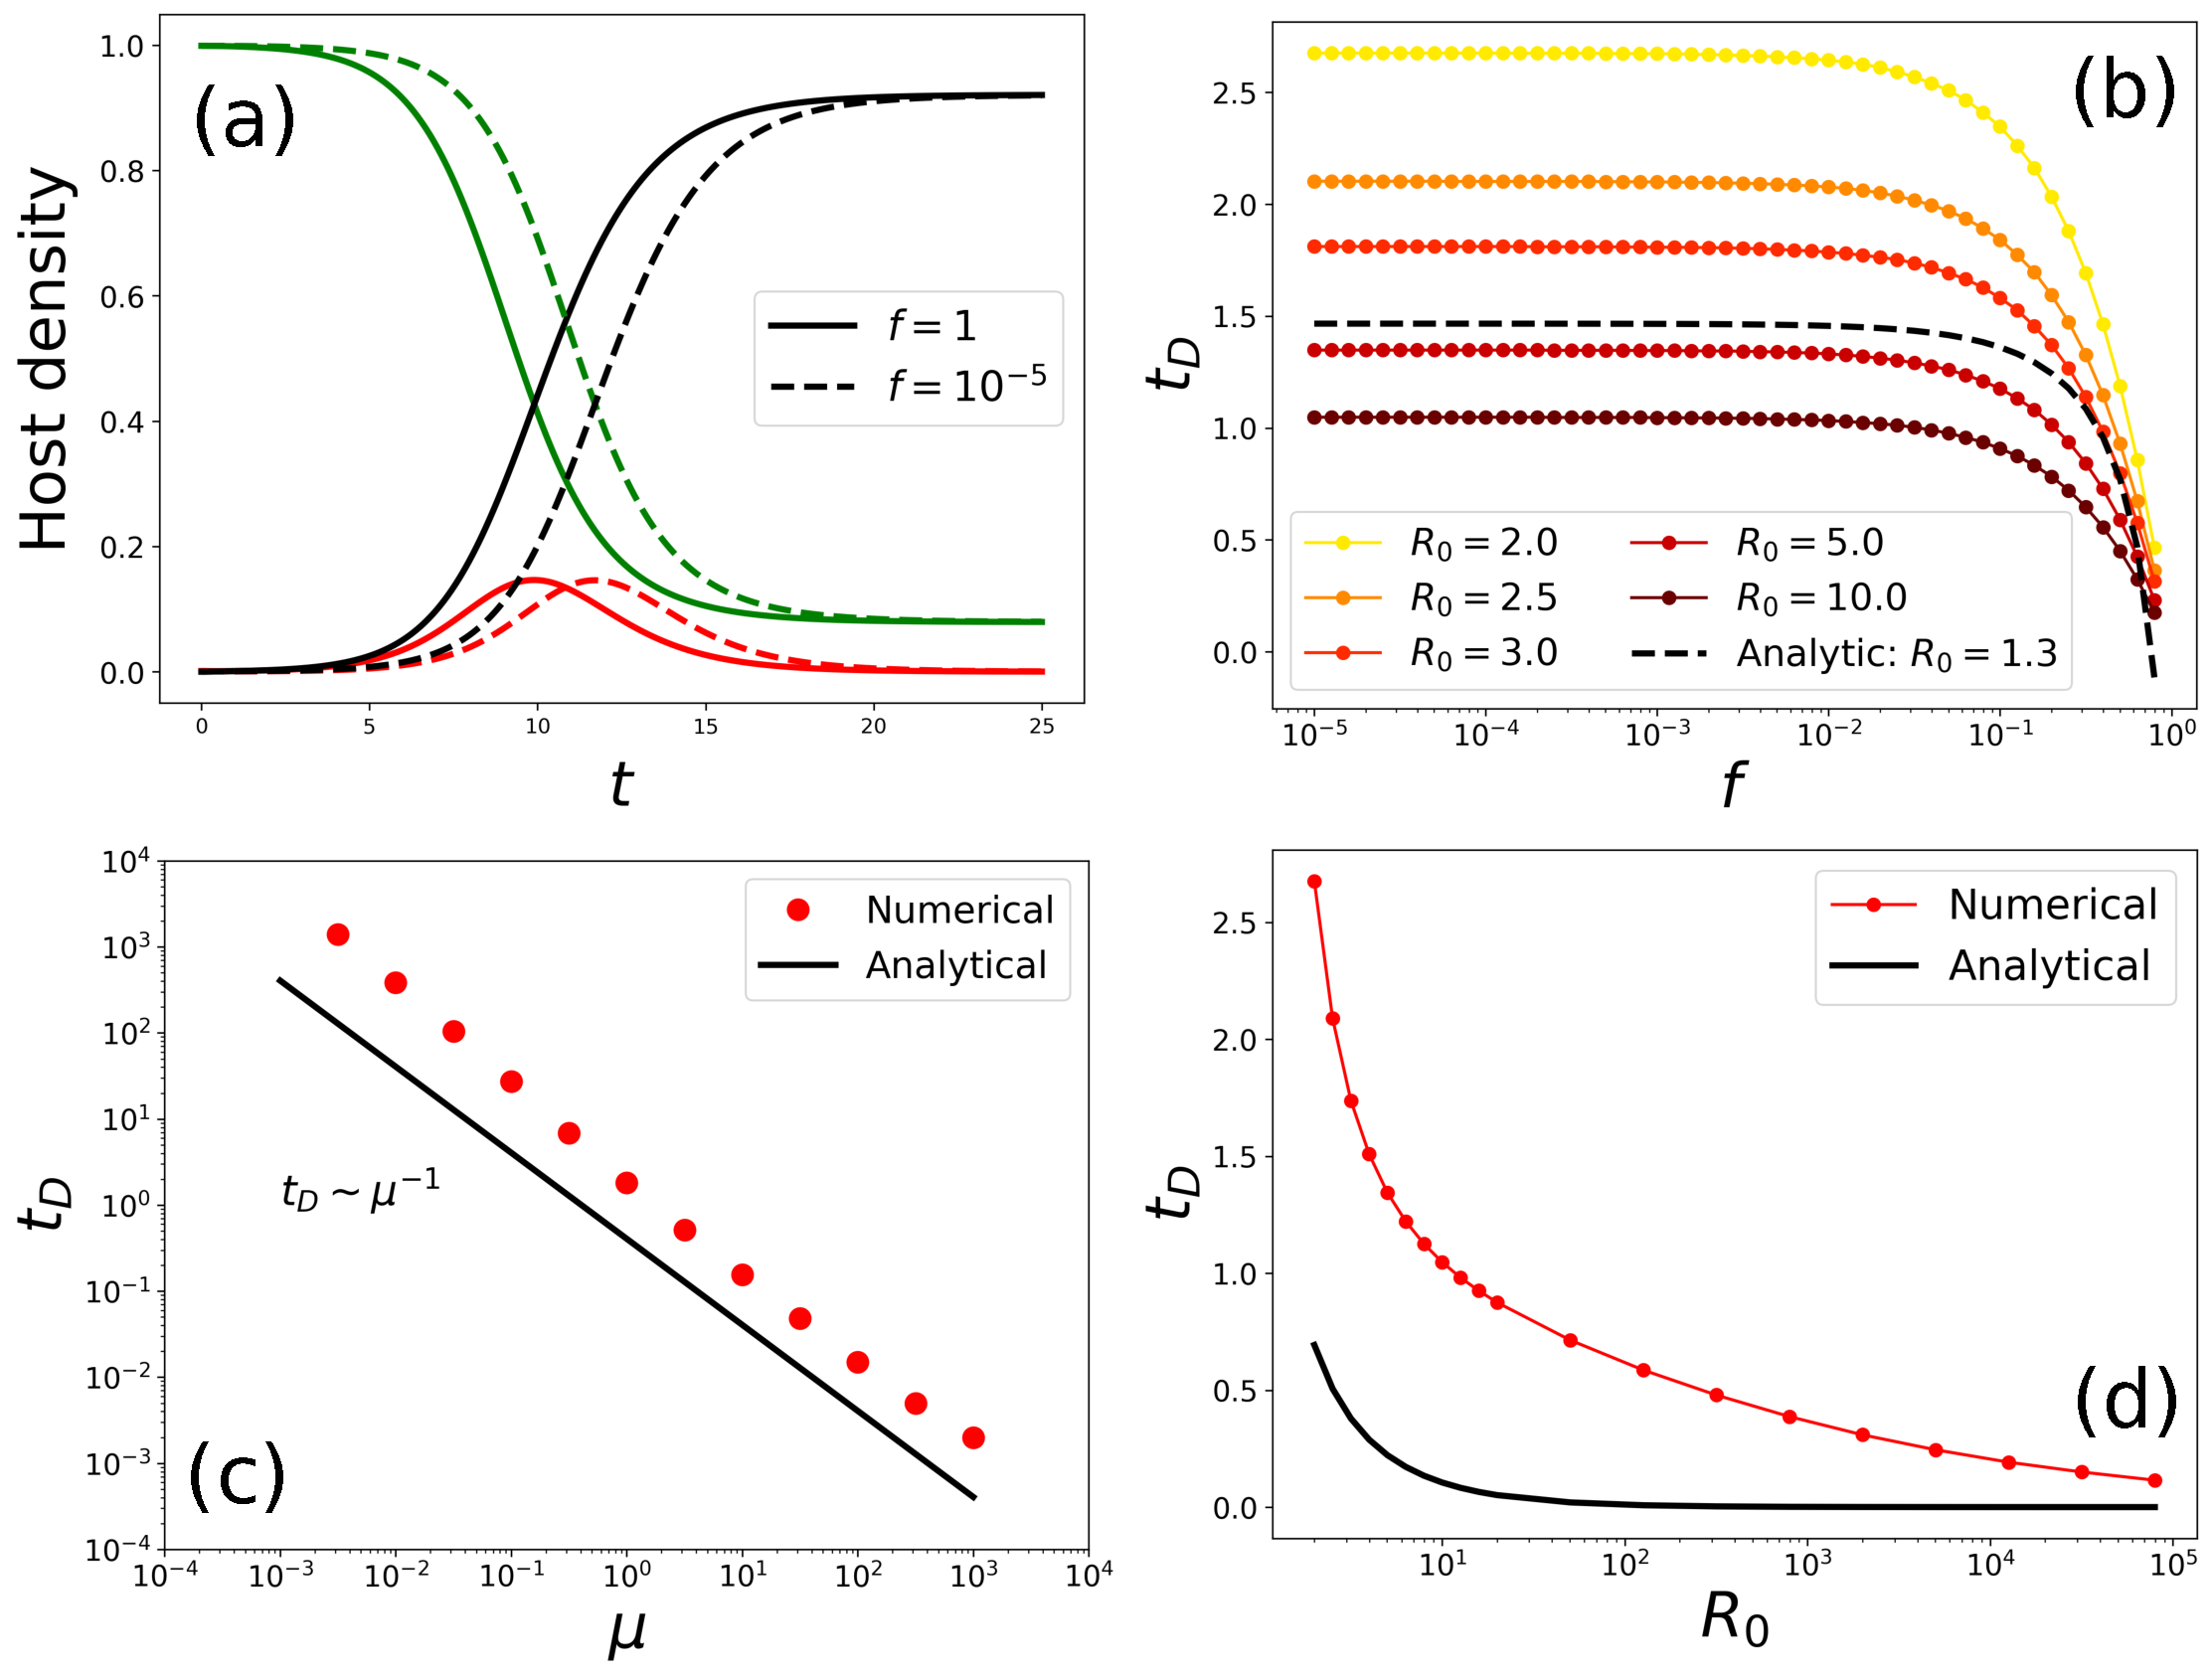
\includegraphics[width=0.8\textwidth]{Figures/delay.pdf}
    \caption{Numerical study of the delay induced by growing vector
    populations. (a) Comparison of hosts dynamics for a stationary vector
    population ($f=1$) and a growing vector population ($f=10^{-5}$). (b) Time
    delay as function of $f$ for different values of the basic reproduction
    number
    $R_0$. (c) Time delay as function of the vector natural death rate. (d)
    Time
    delay as function of the basic reproduction number, $R_0$, with
    $f=10^{-5}$.}
    \label{fig:delay}
\end{figure}

\subsection{The basic reproduction number for non-stationary vector
    populations}

As shown in the previous section, traditional methods to compute the basic
reproduction number fail in the case of epidemic models with decaying vector
populations, $f>1$, unless the time scale of vector population fulfills the
strong inequality condition \cref{eq:timescales_condition}, as illustrated in
\cref{sec:R0statvp}. Here we introduce an effective, average definition of
$R_0$, useful to predict the epidemic onset for vector-borne diseases with
decaying vector populations, i.e. the case where traditional methods fail. It
is defined as the \textit{average} number of infections produced by an infected
individual in \textit{one generation} \cref{eq:generationtime},
\begin{equation}\label{eq:R0_non_stationary}
    \overline{R_0}=\avg{R_{0}^{i}(t)}\Big\rvert\limitss{0}{t_g}=
    R_0\claudator{1-\frac{1}{\tau}\parentesi{f-1}
        \parentesi{e^{-\tau}-1}}=R_0\cdot\mathcal{F}
\end{equation}
where $\tau=1+\mu/\gamma$ and $\mathcal{F}$ accounts for the effect of the
decaying vector population on the stationary $R_0$ (see
\cref{app:R0_non_stationary} for the full derivation of
\cref{eq:R0_non_stationary}).

A first observation is that $\overline{R_0}>R_0$ always (for $f>1$). This
stems from the fact that $\tau=1+\mu/\gamma>1$, so that $e^{-\tau}-1<0$, and
$f-1>0$, which yields $\mathcal{F}>1$. This discussion unravels why standard
methods fail to predict the onset of an epidemic under decaying vector
populations. Another important point is that if $\mu/\gamma\gg 1$, which
implies $\tau\gg1$,
\begin{equation}
    \lim_{\tau\gg1}\mathcal{F}=\lim_{\tau\gg1}\claudator{1-\frac{1}{\tau}
        \parentesi{f-1}\parentesi{e^{-\tau}-1}}=1+\frac{f-1}{\tau}\
    ,
\end{equation}
and if furthermore $\tau\sim\frac{\mu}{\gamma}\gg (f-1)$ then
$\mathcal{F}\to 1$ and $\overline{R_0}\to R_0$. This is in agreement with the
discussion in \cref{sec:R0statvp} showing that the $R_0$ computed from standard
methods works if $\mu\gg\gamma$.

\begin{figure}[H]
    \centering
    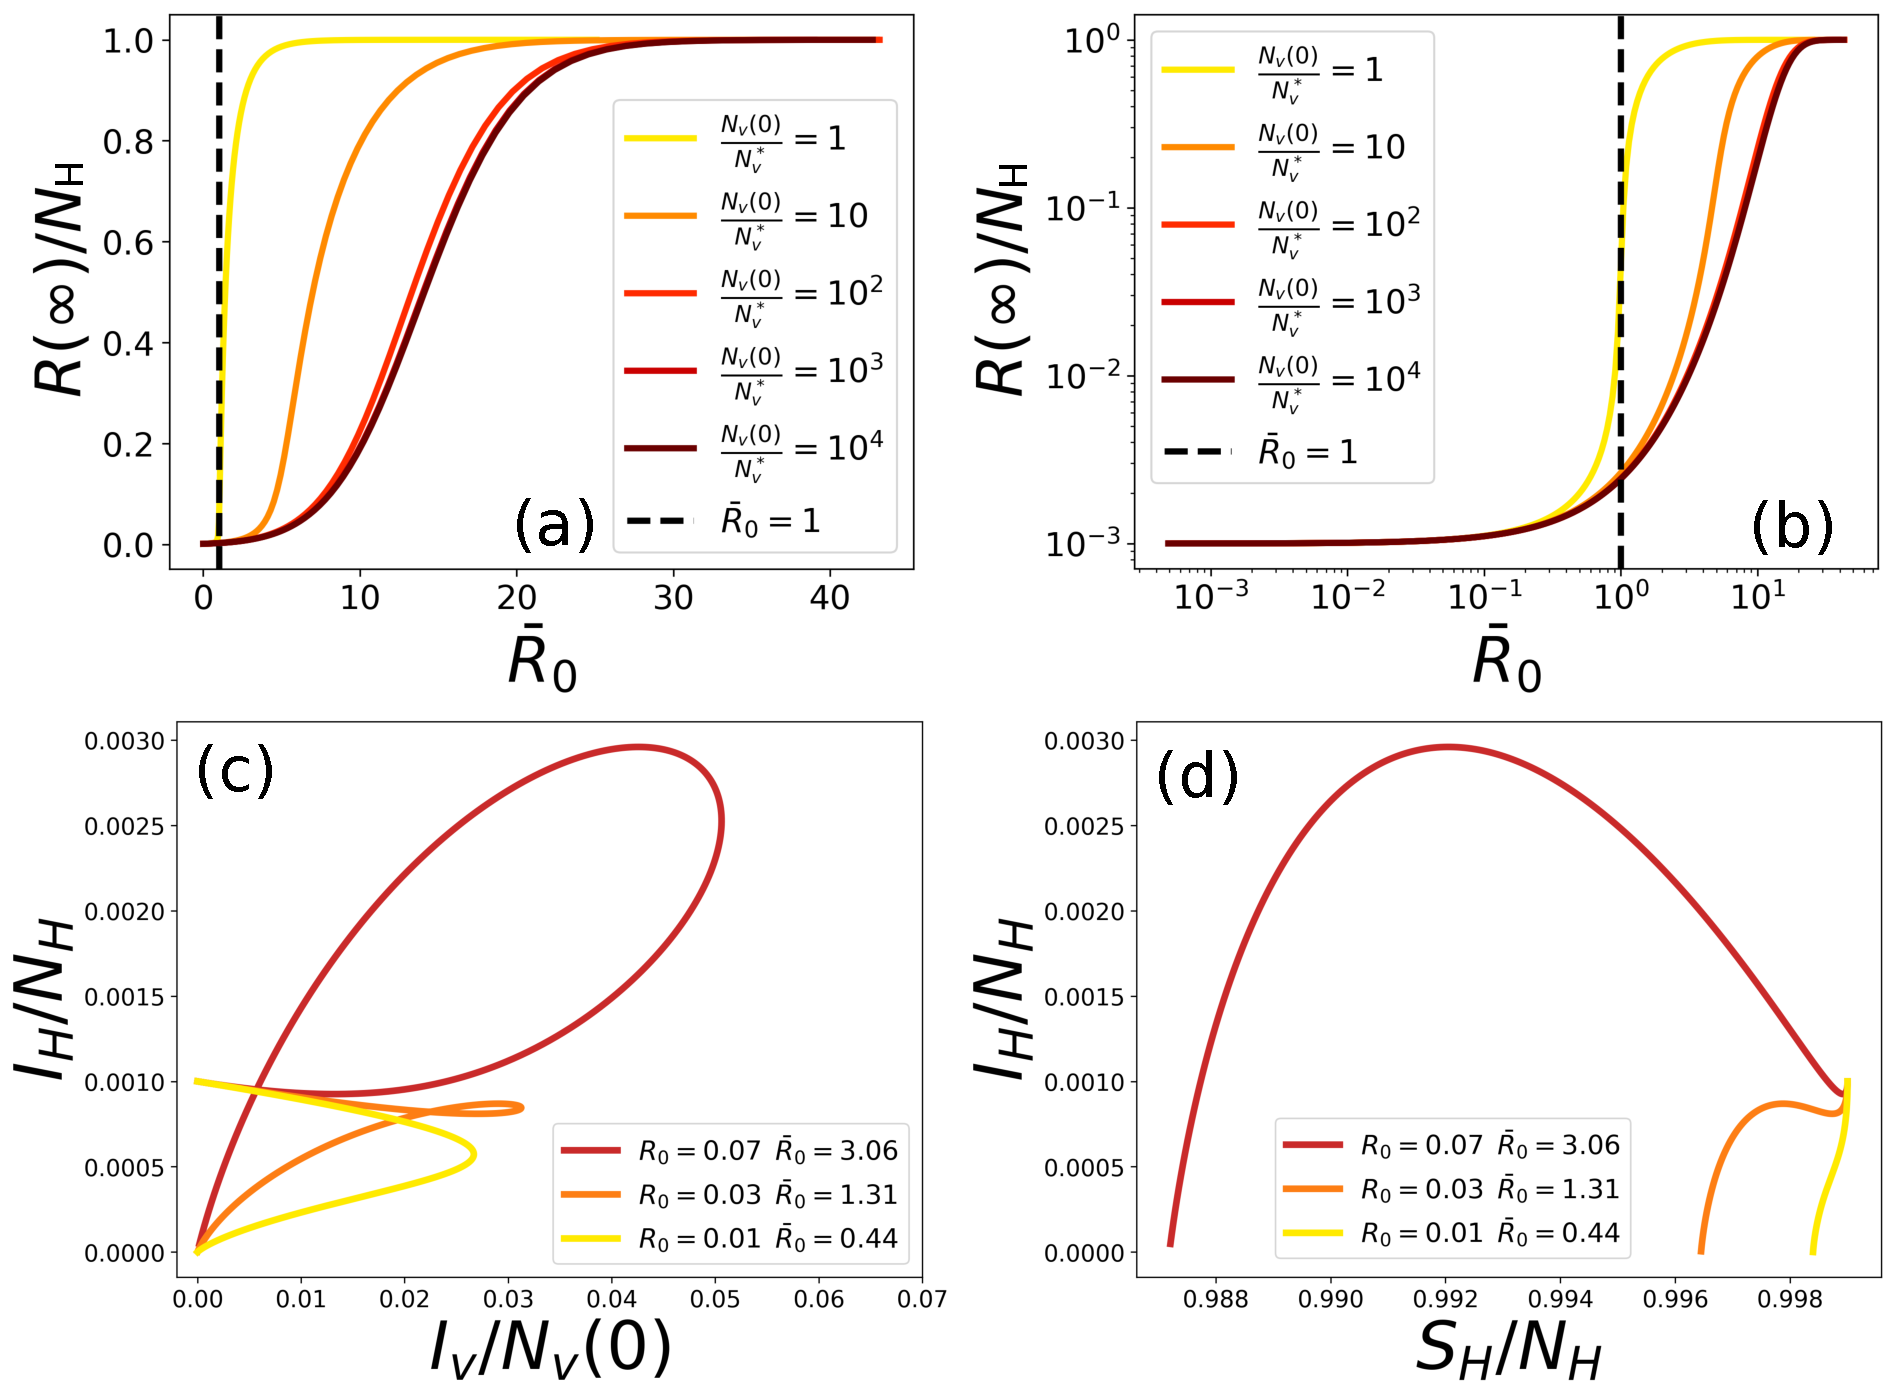
\includegraphics[width=0.8\textwidth]{Figures/R0_check_mean_value.pdf}
    \caption{Numerical verification of the expression for the basic
        reproduction number for vector-borne diseases with decaying vector
        populations
        \cref{eq:R0_non_stationary}. Final size of the epidemic as a function
        of the
        basic reproduction number in panels: (a) linear scale; (b) logarithmic
        scale.
        Phase space trajectories in panels: (c) $I_H/N_H$ vs $I_v/N_v(0)$ and
        (d)
        $I_H/N_H$ vs $S_H/N_H$, where an initial condition $I_H(0)/N_H=0.01,
            S_H(0)/N_H=0.99$ and $I_v(0)/N_V(0)=0$ has been used for the $3$
        cases.
        $\mu=\gamma$ has been used in all the simulations.}
    \label{fig:R0_check_mean_value}
\end{figure}

\cref{fig:R0_check_mean_value}(a-b) contrasts numerically the validity of
\cref{eq:R0_non_stationary} to predict the final size of the epidemic as a
function of the general basic reproduction number, $\overline{R_0}$, in linear
and logarithmic scale, respectively. We observe that, independently of the
initial condition of vectors, the outbreak occurs for $\overline{R_0}>1$.
However, we may notice that for large values of the initial condition of
vectors the final size of the epidemic grows more slowly, so that larger values
of $\overline{R_0}$ are needed to produce a proper outbreak. This can be
explained by the fact that for $\overline{R_0}$ slightly above the threshold,
$\overline{R_0}=1$, and large values of $f=N_v(0)/N_v^*$, infections are
produced only in the transient period of the dynamics, as $R_0<1$. This is,
while the vector population is decaying to its stationary value, the vectors
are able to produce new infections, but once the vector population reaches the
stationary value, the epidemics stops. This transmission mechanism is radically
different to that of vector-borne diseases with stationary vector populations
in which the pre-pandemic disease-free state is an equilibrium of the system.
The phase-space plots in \cref{fig:R0_check_mean_value}(c-d) show that the
time-averaged basic reproduction number $\overline{R_0}$ is able to accurately
predict the conditions under which the infected host population will grow, in
contrast with $R_0$ computed in the post-pandemic fixed point. In essence, for
$\overline{R_0}>1$ the infected host population, $I_H$, grows before reaching
the absorbing state, $I_H=I_v=0$, while for $\overline{R_0}<1$ the infected
host population is monotonically decreasing. We note that
\cref{eq:R0_non_stationary} is similar to the time-averaged basic reproduction
number presented in \cite{Wesley2009} for the periodic case, which is a
first-order approximation to the \textit{true} basic reproductive number
\cite{Bacaer2006}.

\subsection{Fast-slow approximation}

The original $5$-D \cref{eq:SIR_v} model is certainly not amenable to
mathematical analyses due to its high phase-space dimensionality and the fact
that it depends on $4$ parameters. Moreover, in a real-case application, if the
parameters conforming the model are not known, the model could suffer from
parameter unidentifiability. However, some approximations can be performed to
reduce the mathematical complexity of the model, as for instance a fast-slow
(or adiabatic) approximation.

If the time-scale of the vector population evolution is much faster than
that of the infected hosts, what is expected to be a good approximation in many
practical cases, the vector population will almost instantaneously adapt to its
stationary value. Thus, if $1/\mu\ll1/\gamma$, or equivalently if
$\gamma/\mu\ll1$, we can rewrite the time derivative of the vector infected
population as
\begin{equation}
    \epsilon\dot{I}_v=\frac{\alpha}{\mu}S_v\frac{I_H}{N_H} - I_v \ ,
\end{equation}
where time has been re-scaled to $t'\to\gamma t$ and $\epsilon=\gamma/\mu$
is a small parameter. Then, $\dot{I_v}$ can be neglected and the infected
vector population can be obtained from the relationship,
\begin{equation}\label{eq:Iv_timescale_approx}
    I_v\approx\frac{\alpha}{\mu}\frac{S_v I_H}{N_H} \ .
\end{equation}

Substituting \cref{eq:Iv_timescale_approx} into the original system
\cref{eq:SIR_v} and the identity $N_v(t)=S_v(t)+I_v(t)$, while considering that
the conditions for which the time-scale approximation is valid, $\mu\gg\gamma$,
imply that the vector population will reach its stationary value almost
instantaneously, so that $N_v(t)\approx N_v^*$, we obtain the following reduced
system,
\begin{equation}\label{eq:SIR_like}
    \begin{aligned}
        \dot{S}_H & =-\beta'\frac{S_H I_H}{\lambda N_H + I_H}            \\
        \dot{I}_H & =\beta'\frac{S_H I_H}{\lambda N_H + I_H}- \gamma I_H \\
        \dot{R}_H & =\gamma I_H \ ,
    \end{aligned}
\end{equation}
where $\beta'=\beta N_v^*/N_H$ and $\lambda=\mu/\alpha$.

Moreover, if $f\neq1$ the above mentioned timescales relationship
must fulfil
$\displaystyle\frac{\mu}{\gamma}\gg\abs{\ln{\frac{\epsilon}{f-1}}}$ (cf.
\cref{eq:timescales_condition}) and not only
$\displaystyle\frac{\mu}{\gamma}\gg 1$. It is important to notice that the
presence of direct host to host transmission would simply re-scale the
coefficient $\beta'$, and the SIR reduction \cref{eq:SIR_like} would keep its
validity.

\begin{figure}[H]
    \centering
    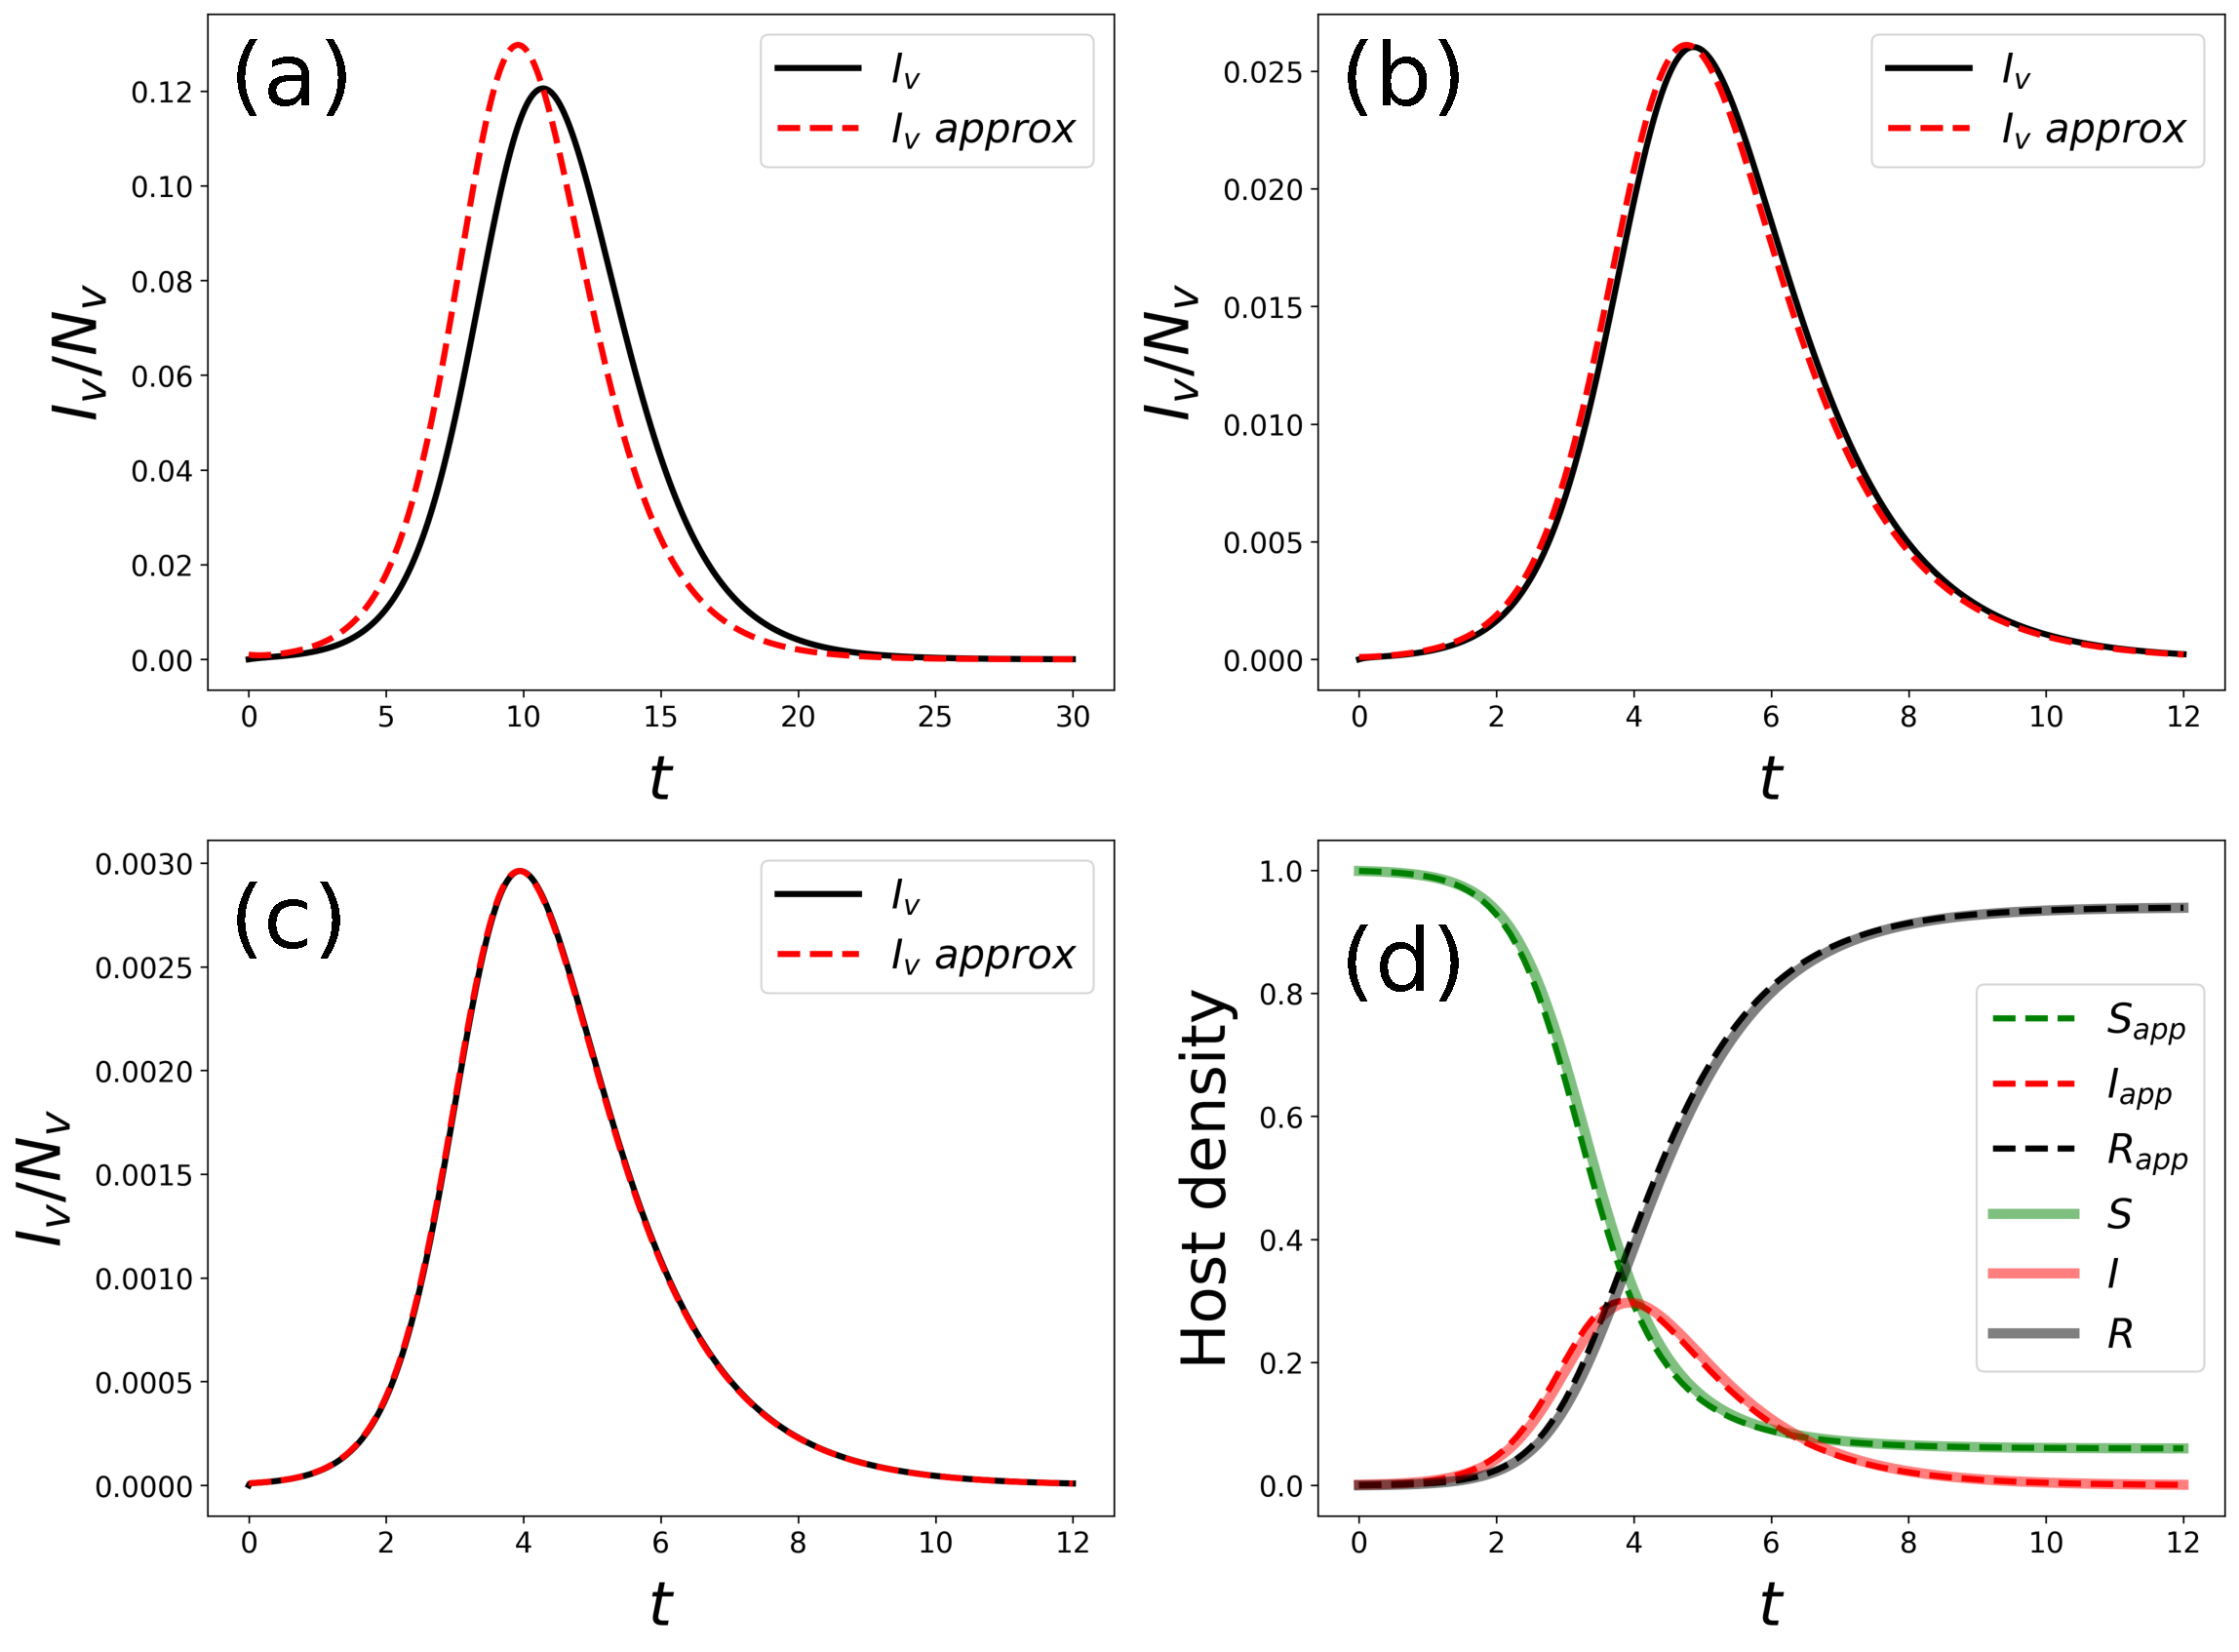
\includegraphics[width=0.8\textwidth]{Figures/Timescale_approx.pdf}
    \caption{Numerical verification of the time-scale approximation
        (\cref{eq:Iv_timescale_approx}) with $N_H=100$, $\alpha=\gamma=1$.
        $\beta$ is
        chosen such that $R_0=3$. (a) $\mu=1$, (b) $\mu=10$, (c) $\mu=100$.
        Panel (d)
        shows a comparison between the approximate and original models for the
        parameters used in (c), where the approximated models is expected to
        represent
        well the original one.}
    \label{fig:timescale_approx}
\end{figure}

In \cref{fig:timescale_approx} we numerically verify the validity of the
presented fast-slow approximation. As expected, we observe that the
approximation breaks down for $\mu\sim\gamma$ (\cref{fig:timescale_approx}(a)),
while as
$\mu$ becomes larger than $\gamma$ the approximation improves
\cref{fig:timescale_approx}(b) and it becomes quantitative when $\mu\gg\gamma$,
\cref{fig:timescale_approx}(c). Finally, we show in
\cref{fig:timescale_approx}(d) a comparison between the dynamics of the hosts
using both the original and the approximated model using the same parameters
than in \cref{fig:timescale_approx}(c), where the results of both models are
expected to converge.

\subsection{Reduction to a SIR model}

In addition to the previous condition, $\gamma/\mu\ll1$, if one has that
$\lambda N_H \gg I_H$ also holds (which is indeed plausible in this limit)
\cref{eq:SIR_like}, then the model can be written as a standard SIR model,
\begin{equation}\label{eq:SIR}
    \begin{aligned}
        \dot{S}_H & =-\beta_{eff}\frac{S_HI_H}{N_H}            \\
        \dot{I}_H & =\beta_{eff}\frac{S_HI_H}{N_H}- \gamma I_H \\
        \dot{R}_H & =\gamma I_H \ ,
    \end{aligned}
\end{equation}
where $\displaystyle\beta_{eff}=\frac{\beta'}{\lambda}=\frac{\beta\alpha
        N_v^*}{\mu N_H}$.

\begin{figure*}[t!]
    \centering
    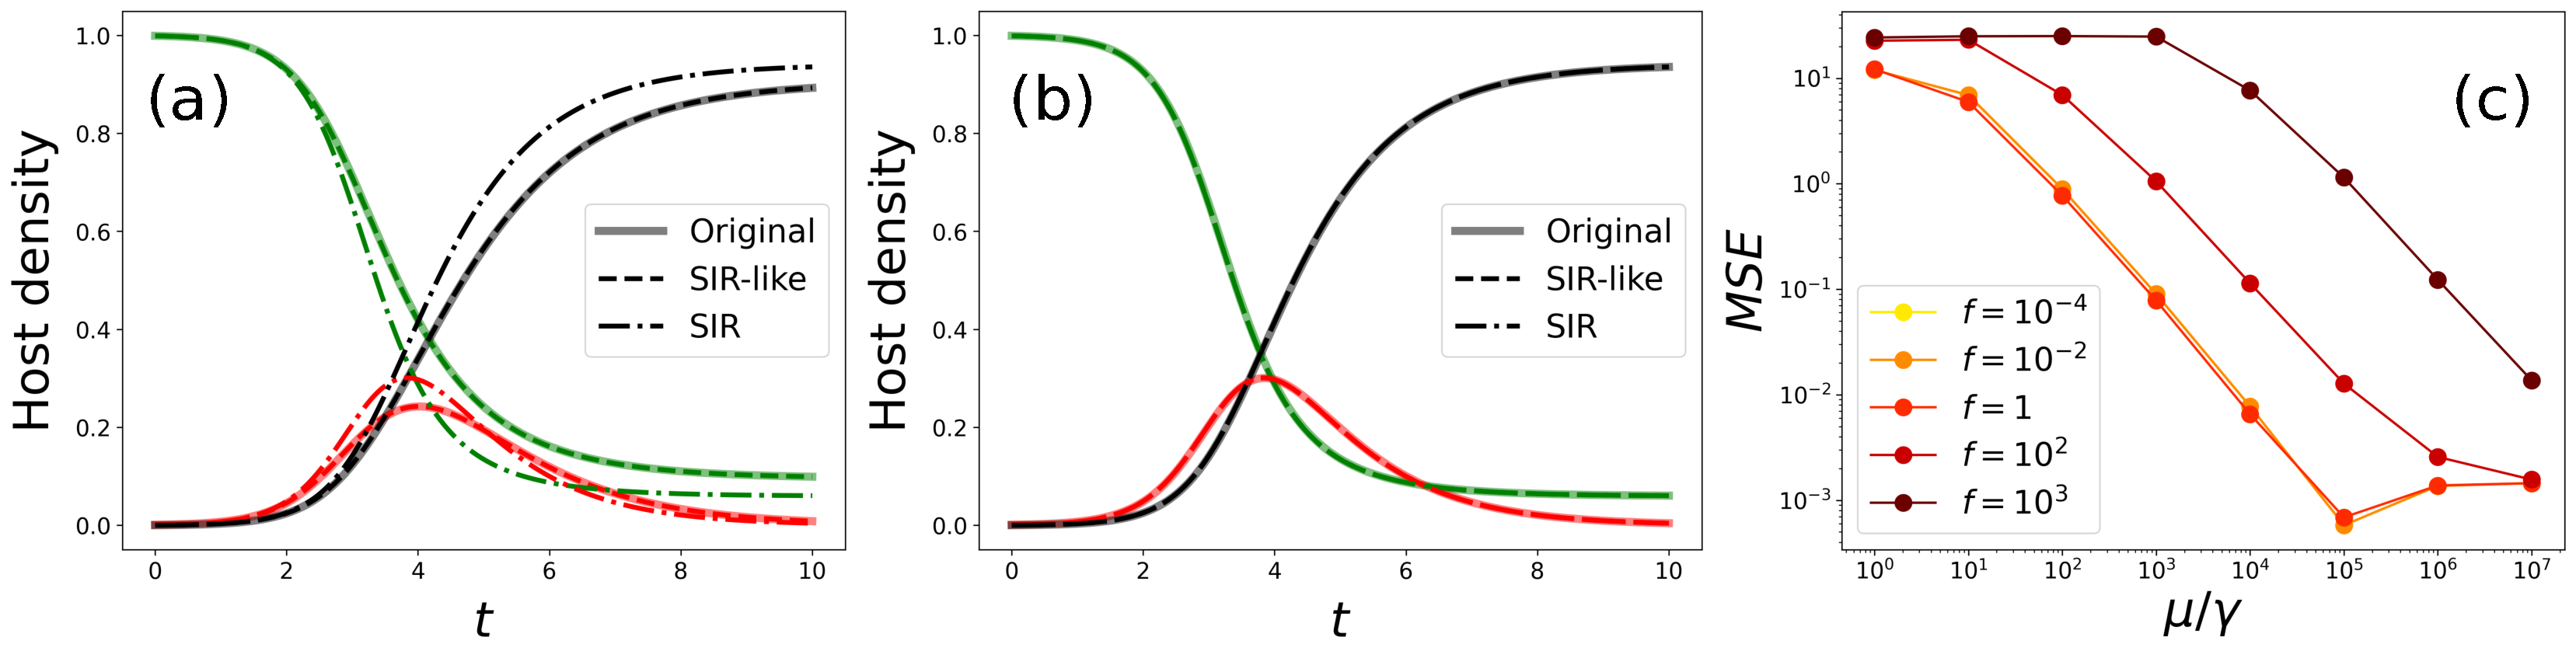
\includegraphics[width=\textwidth]{Figures/SIR_like_approx_comp.pdf}
    \caption{Comparison between the original model and the reductions,
    \cref{eq:SIR_like} (SIR-like) and \cref{eq:SIR} (SIR) with $N=100$,
    $\mu/\gamma=10^{3}$ and $f=1$. $\beta$ was chosen such that $R_0=3$.  (a)
    $\lambda=1$, (b) $\lambda=10^3$, (c) Mean Squared Error between the
    original
    model and the SIR approximations as function of the ratio $\mu/\gamma$ and
    $f$.}
    \label{fig:SIR_like_approx}
\end{figure*}

In \cref{fig:SIR_like_approx} we show the validity of the reduced models
\cref{eq:SIR_like} and \cref{eq:SIR}. \cref{fig:SIR_like_approx}(a) shows that
the SIR-like model (\cref{eq:SIR_like}) works when the time-scale approximation
can be performed (as $\mu/\gamma\gg1$) but the SIR model fails when the
condition $\lambda N_H \gg I_H$ is not fulfilled. Conversely, in
\cref{fig:SIR_like_approx}(b) we show that as $\lambda N_H \gg I_H$ is
fulfilled, then the SIR model perfectly matches the original model. Finally,
\cref{fig:SIR_like_approx}(c) shows the decrease in the mean squared error of
the approximation as the condition \cref{eq:timescales_condition} is fulfilled
for different values of $f$.

\section{Conclusions}\label{sec:conclusions}

In the present work we have analyzed several features of a compartmental
deterministic model for vector-borne diseases with $3$ compartments for hosts
and $2$ for vectors, that does not consider neither direct host to host nor
vertical transmission. The goal is to study the behavior of the model in the
case that the vector population is not stationary. In this case, the
pre-pandemic disease-free state is not a fixed point (equilibrium state) of the
dynamical system, and, in principle, the methods that are customarily used to
determine the basic reproduction number, $R_0$ do not work. This is so because
these methods determine the onset of an outbreak by performing a linear
stability analysis of the disease-free state, assuming that it is a fixed point
of the model. A common assumption made in the literature is to determine $R_0$
from the asymptotic state for the vectors (if it is not an extinction state), a
fixed point of the model.

We have analyzed several initial conditions of the vector population,
characterizing different regimes. In the case that the initial condition for
the number of vectors is below the asymptotic state, implying that the vector
population overall grows, then $R_0$ as determined from the asymptotic state
correctly predicts the existence (or not) of an epidemic outbreak, but with a
temporal delay in its appearance. This result contrasts with the situation in
which the initial state is above the asymptotic state, with an overall decrease
in the vector population. In this case $R_0$ determined from the asymptotic
state may fail badly, predicting no outbreak while a large fraction of the
population might get infected. We present a simple, albeit useful,
generalization of $R_0$ that is able to give a reasonable prediction of the
epidemic threshold for decaying populations, including the case in which
vectors become extinct, a case in which the asymptotic estimation to determine
$R_0$ cannot be applied.

Compartmental models of vector-borne diseases usually have many
compartments and parameters, which can lead to a problem of parameter
unidentifiability. The model analyzed here is not an exception, and when
applied to real-world cases many different combinations of the parameters could
be able to reproduce the available data. Thus, in order to facilitate the
application of the model to experimental data, we have studied a useful
fast-slow (or adiabatic) approximation that allows to reduce the model if the
parameters fulfill certain conditions. In particular, our study shows that
under quite realistic assumptions (the typical timescale of hosts infection and
death is much slower than vector timescales) it is possible to obtain a reduced
SIR model. We recall that this reduction implies that, under these assumptions,
the process by which hosts (that could be immobile) get infected through the
action of vectors is equivalent to a direct interaction among hosts.

The deterministic compartmental model analyzed here, with some
modifications, is a clear candidate to study many vector-borne diseases, in
particular phytopathologies. Furthermore, in case of parameter
unidientifiability the model reductions performed in this work could be useful
to solve this issue. In any case, this description is still idealized, as
compartmental models imply a well-mixed assumption in which space is not
explicitly described. This kind of representations are not always applicable to
real-world scenarios although are useful as a first approximation. Thus, future
research should focus on the integration of space and vector mobility in the
model to account for more realistic situations.

%----------------------------------------------------------------------------------------
%	A compartmental model for Xylella fastidiosa diseases with explicit
%   vector seasonal dynamics
%----------------------------------------------------------------------------------------
\chapterimage{almond.jpg}
\chapterspaceabove{6.75cm}
\chapterspacebelow{7.25cm}

\chapter{A compartmental model for \textit{Xylella fastidiosa} diseases}
\vspace{3cm}

% \textbf{Àlex Giménez-Romero$^{1}$, Eduardo Moralejo$^{2}$, Manuel A.
%     Matías$^{1}$}

% \vspace{1cm}

% \begin{enumerate}
%     \small
%     \item Instituto de Física Interdisciplinar y Sistemas Complejos, IFISC
%           (CSIC-UIB), Palma de Mallorca 07122, Spain
%     \item Tragsa, Passatge Cala Figuera 6, 07009 Palma de Mallorca, Spain
% \end{enumerate}

% \vspace{1cm}

\textbf{Published as}

\vspace{0.5cm}

\fullcite{GimenezRomero2023}

\newpage
\section{Introduction}

Mathematical and computational modeling in Ecology and, in particular,
Epidemiology have been recently recognized as powerful approaches to guide
empirical work and provide a framework for the synthesis, analysis and
development of conservation plans and policy-making
\cite{levin1992mathematics,Murray_book,sarkar2006biodiversity,Chew2014}.
Plant epidemics, mainly plant-virus diseases, have been often described by
compartmental models, which deal with the overriding importance of transmission
mechanisms in determining epidemic dynamics
\cite{Jeger1998,Jeger2004,Madden2000}. These models have contributed to
providing answers to some questions related to the ecology of plant diseases
and have led to direct applications in disease control while guiding research
directions \cite{Jeger2019}.

The emergence of vector-borne plant pathogens in new areas causing huge
economic impacts, such as \textit{Xylella fastidiosa} and the
\textit{Candidatus} Liberibacter spp. (Huanglongbing or citrus greening), has
sparked interest in modeling vector-transmitted plant-disease epidemics
\cite{chiyaka2012modeling,Jeger2019}. The vector-borne bacterium \textit{X.
    fastidiosa} (Xf) is a multi-host pathogen endemic to the Americas that
causes
economically important diseases, mostly in woody crops \cite{Hopkins2002}. Xf
is a genetically diverse species with three evolutionary well-defined clades
forming the \textit{pauca}, \textit{fastidiosa}, and \textit{multiplex}
subspecies, native from South, Central, and North America, respectively
\cite{vanhove2019genomic}. Within each subspecies, diverse genetic lineages
with different host ranges are found. Xf is transmitted non-specifically by
xylem-sap-feeding insects belonging to the sharpshooter leafhoppers (Hemiptera:
Cicadellidae, Cicadellinae) and spittlebugs (Hemiptera: Cercopoidae)
\cite{Redak2004}.

Recently, Xf has gained renewed interest due to the massive mortality of
olive trees in Apulia, Italy \cite{saponari2019xylella}. The first focus of
the olive quick decline syndrome (OQDS) was detected in 2013 around Gallipoli
(Apulia, Italy)\cite{saponari2013identification} and since then has spread
throughout the region by the meadow spittlebug, \textit{Philaenus spumarius}.
Although this was the first official detection of Xf in Europe, it has recently
been demonstrated that the pathogen arrived much earlier in Corsica
\cite{Soubeyrand2018} and in the Balearic islands \cite{Moralejo2020}.
Around 1993, two strains of the subspecies \textit{fastidiosa} (ST1) and
\textit{multiplex} (ST81) were introduced from California to Mallorca (Spain)
with infected almond plants \cite{Moralejo2020}. To date, over 80\% of the
almond trees in Mallorca show leaf scorch symptoms and the outbreak has changed
the iconic rural landscape of this Mediterranean island \cite{Olmo2021b}.

The meadow spittlebug,	\textit{P. spumarius} (Hemiptera: Aphrophoridae),
has recently been shown to be the main vector of Xf in Europe both in
transmission experiments and in field studies
\cite{Cornara2017,Cornara2018,lopez2022mechanical,Moralejo2019,saponari2019xylella}.
\textit{P. spumarius} is a polyphagous species from the Palearctic region,
presenting one generation per year (univoltine) and overwintering as eggs.
Foam-forming nymphs emerge at the end of winter, feeding on herbaceous plants.
The time required for their development to the adult stage depends mainly on
temperature and humidity
\cite{bodino2019phenology,Chmiel1979,cornara2018philaenus}. In Mediterranean
climates,  \textit{P. spumarius} adults generally move from the herbaceous
cover to the crop canopy as evapotranspiration increases in late spring
(May–June). In mid-summer, the populations of \textit{P. spumarius} tend to
decrease in the crop canopy, while the insects are captured more frequently in
trees and shrubs interspersed in crops. Summer dispersal of spittlebugs to wild
hosts as refugee seems a common general pattern in Mediterranean crops in Italy
\cite{bodino2019phenology,cornara2021natural} and Spain
\cite{morente2018distribution}. Because the bacterium has not been detected
in spring on insects feeding on the herbaceous cover or in weeds in Europe
\cite{bodino2019phenology,cornara2018philaenus,Olmo2021b}, it is assumed that
all spittlebug adults acquire the bacteria from the main crop (olive, almond,
vine, etc.). Once infected, Xf colonizes the insect foregut in a persistent and
non-circulatory manner without transovarial (parent to offspring) or
transstadial (inter-stage) transmission
\cite{Almeida2003,freitag1951host,purcell1979evidence} and without
a period latency after vector acquisition \cite{Almeida2015,freitag1951host}.

Several epidemic models have been already developed for Xf-diseases, but
they lack a realistic description of some relevant processes
\cite{Jeger2019}. Some of these models assume a simple general form for
infected host dynamics \cite{White2017,Abboud2019,Daugherty2019} or use a
simplified S-I compartmental scheme for hosts, disregarding important features
such as the latent period or the host mortality rate \cite{Soubeyrand2018}.
Models that do take these features into account, however, do not explicitly
model the population of vectors responsible for disease transmission
\cite{White2020}. Other more recent models have taken a step further in
explicitly modeling the vector population \cite{BRUNETTI2020,
    GimenezRomero2022_CommsBio}, but the characterization of its dynamics is
still
relatively simple, as it overlooks the known seasonal patterns of vector
abundance. Several recent studies have provided new insights into the ecology
and temporal dynamics of the transmission of Xf by \textit{P. spumarius} in
olive plants \cite{Bodino2021,bodino2019phenology}. However, these
experimental data of the pathosystem have not been yet integrated at the
population level. Thus, there is a need to continue advancing in the modeling
of Xf diseases by developing more realistic models that can elucidate the
fundamental processes involved in vector-host-pathogen interactions and help to
design effective control strategies.

In this work, we develop a deterministic continuous-time compartmental
model to describe the general epidemiological dynamics of diseases produced by
Xf in Europe. We explicitly account for key biological aspects of the disease,
including the seasonal dynamics of its main vector, \textit{P. spumarius}. Our
model is able to describe field data from the two major European outbreaks: the
olive quick disease syndrome (OQDS) in Apulia, Italy, caused by the subspecies
\textit{pauca}, and the almond leaf scorch disease (ALSD) in Mallorca, Spain,
caused by subspecies \textit{multiplex} and \textit{fastidiosa}. We aimed to
find the most influential parameters in the model with respect to incidence and
mortality in both diseases by performing a global sensibility analysis. With
this information, the next goal was to explore control strategies acting
especially on the vector population.

\section{Materials and Methods}

\subsection{Epidemic model: the SEIR-V model}

We developed a deterministic continuous-time compartmental model that
incorporates the specific biological features of Xf diseases in Europe,
including the dynamics of the main relevant vector \textit{P. spumarius}
\cite{Cavalieri2019}. To build the model we took the following
considerations: (i) we assume there is no winter recovery of infected hosts and
thus they die sometime after infection; (ii) hosts show an asymptomatic period
in which they are non-infectious in practice (exposed compartment) because the
bacteria are not yet systemically extended
\cite{teviotdale2003almond,Stevenson238}, while vectors are infectious
immediately after acquiring the bacterium \cite{Fierro2019}; (iii) vectors
have an annual life cycle without mother-to-offspring disease transmission
\cite{freitag1951host,purcell1979evidence}, so we consider the annual
emergence of susceptible newborn vectors and a constant death rate for both
susceptible and infected vectors; (iv) infected vectors carry the bacterium
during their entire lifespan without affecting their fitness; and finally, (v)
we do not consider host recruitment or natural death given that the typical
development time of Xf-epidemics is faster than the typical host's life cycle.

Altogether, our deterministic continuous-time compartmental model consists
of six compartments, four describing the host population (susceptible, $S_H$,
exposed, $E_H$, infectious, $I_H$, and removed, $R_H$), and two describing the
vector population (susceptible, $S_V$, and infected, $I_V$). The model is
defined according to the following processes,
\begin{equation}\label{eq:scheme_infection_phyto}
    \begin{aligned}
         & S_H+I_V \stackrel{\beta}{\rightarrow} E_H + I_V, \quad
        E_H \stackrel{\kappa}{\rightarrow} I_H, \quad
        I_H  \stackrel{\gamma}{\rightarrow} R_H                      \\
         & S_V+I_H \stackrel{\alpha}{\rightarrow} I_V+I_H, \quad S_V
        \stackrel{\mu}{\rightarrow} \varnothing, \quad I_V
        \stackrel{\mu}{\rightarrow}
        \varnothing
        \ ,
    \end{aligned}
\end{equation}
which are illustrated in \cref{fig:model_diagram_phyto}, being the birth of new
susceptible vectors described as a source term.
Thus, the host-vector compartmental model is written as,
\begin{equation}\label{eq:SEIR_v}
    \begin{aligned}
        \dot{S}_H & =-\beta S_H I_v / N_H                                   \\
        \dot{E}_H & =\beta S_H I_v / N_H - \kappa E_H                       \\
        \dot{I}_H & =\kappa E_H - \gamma I_H                                \\
        \dot{R}_H & =\gamma I_H                                             \\
        \dot{S}_v & = N_v(0)\sum_{n=1}^{\infty}\delta(t-nT) -\alpha S_v I_H
        / N_H - \mu S_v                                                     \\
        \dot{I}_v & =\alpha S_v I_H / N_H - \mu I_v \ .
    \end{aligned}
\end{equation}

\begin{figure}
    \centering
    \label{fig:model_diagram_phyto}
    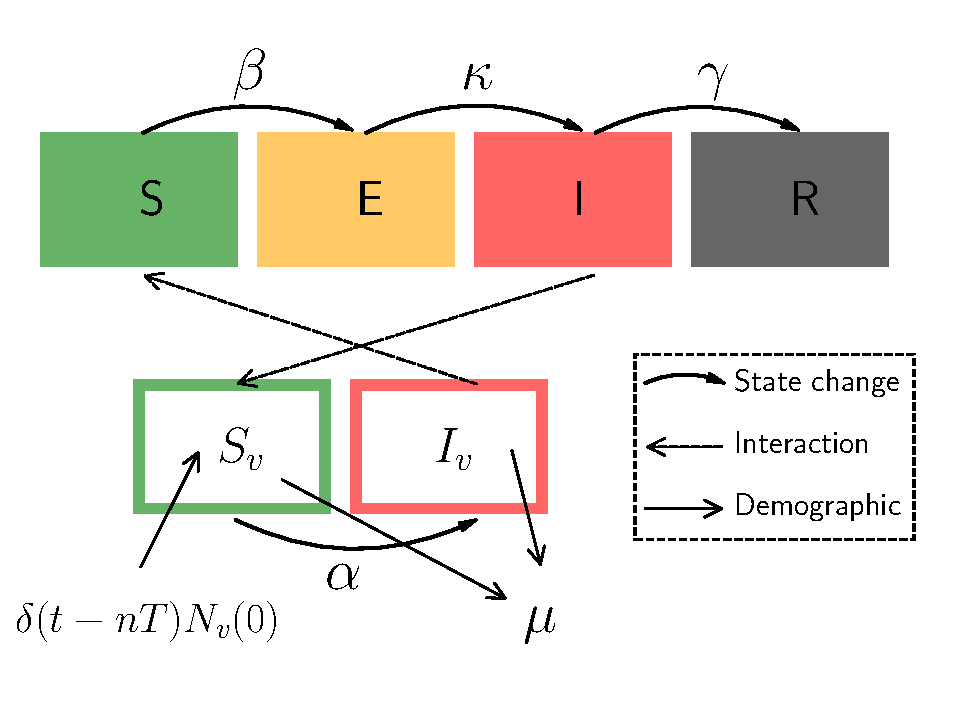
\includegraphics[width=0.8\textwidth]{Figures/SEIR_v_scheme.pdf}
    \caption[Schematic representation of the model]{Schematic representation of
        the model \cref{eq:SEIR_v}. Boxes
        are the compartments in which the population is divided, solid curved
        arrows
        represent changes in state, i.e. transitions between compartments,
        dashed
        arrows depict the crossed interaction between hosts and vectors and
        solid
        straight arrows represent demographic changes in vector population.}
\end{figure}

The model describes the exposure of susceptible hosts, $S_H$, at a rate
$\beta$ through their interaction with infected vectors, $I_v$, while
susceptible vectors, $S_v$, get infected immediately at a rate $\alpha$ through
their interaction with infectious hosts $I_H$. Exposed hosts get infectious at
rate $\kappa$, being the mean latent period $\tau_E=1/\kappa$, while infectious
hosts die at rate $\gamma$, having a mean infectious period of
$\tau_I=1/\gamma$. Infected vectors stay infected and infectious for the rest
of their lifetime. Regarding the seasonal dynamics of vectors, we assume that
new adults emerge synchronously each year in fields being all susceptible. This
is represented by the term $N_v(0)\sum_{n=1}^{\infty}\delta(t-nT)$ in
\cref{eq:SEIR_v}, where $T=\SI{1}{yr}$ is the period and $\delta(t-nT)$ is
Dirac delta function, and basically implements a yearly pulse of new vectors at
a certain moment in the year. Vectors are removed (die, move to herbaceous
vegetation and other non-host trees, exit the field, etc) at a given rate
$\mu$, which we consider identical for susceptible and infected vectors. For
simplicity, we consider that the quantity of annual newborn adults, $N_v(0)$,
is constant. This outburst of new adults followed by an exponential decay
resembles the temporal patterns on the abundance of \textit{P. spumarius}
observed in crop fields  \cite{Antonatos2021,Beal2021,Cornara2017,Lopez2021}
(see \cref{fig:vector_dynamics}).

In our model (\cref{eq:SEIR_v}) the crossed nonlinear terms in $\dot{S}_H$
and $\dot{S}_v$, $S_H I_v$ and $S_v I_H$, are divided by the total host
population, $N_H$. Thus, the vector-to-plant infection process is modeled using
mass action incidence, which is density dependent, while the plant-to-vector
infection process is modeled using standard incidence, which is frequency
dependent \cite{MartchevaBook}. This implies that doubling the number of
vectors in the crop field would double the number of resulting exposed (or
infected) hosts, as this process is population-dependent (mass action
incidence), while doubling the number of hosts would not result in more vectors
per unit area being infected, as this process only depends on the contact
probability, being frequency dependent (standard incidence). We think this is
the most reasonable assumption because, for a given plantation framework,
increasing the number of hosts is expected to also increase the area of the
field, while the number of vectors is an independent quantity.

\subsection{Basic reproductive number}

The basic reproductive number, $R_0$, of the model cannot be trivially
computed using standard methods such as the Next Generation Matrix (NGM)
\cite{Diekmann2010}, as there is no pre-pandemic fixed point in the system of
differential equations \cref{eq:SEIR_v}. For periodically varying vector
populations, rigorous methods have been developed \cite{Bacaer2007}, but not
for the case of growing or decaying vector populations. Here we use the simple
method developed in \cref{ch:xf_PRE} \cite{GimenezRomero2022_PRE} (see
\cref{app:R0}), which
effectively computes the average number of secondary infections produced by an
initially infectious individual in one generation. Thus, the effective basic
reproductive number is given by
\begin{equation}\label{eq:R0}
    R_0=\frac{\beta\alpha}{\mu\gamma}\frac{S_H(0)}{{N_H}^2}
    \frac{N_v(0)}{\mu\tau}\left(1-e^{-\mu\tau}\right)
    \ ,
\end{equation}
where $\tau$ corresponds to the time length of one generation, in our case
one year. This $R_0$ is calculated using the initial susceptible host
population, $S_H(0)$. Below we will also use a time-dependent $R_0(t)$ using
$S_H(t)$.

\subsection{Epidemiological data}

Epidemiological data from an ALSD outbreak in the island of Mallorca,
Balearic Islands, Spain were taken from \cite{Moralejo2020}. Dated phylogenetic
analysis and estimates of disease incidence showed that the introduction of
both subspecies occurred around 1993 and $\sim 79$\% almond trees were infected
in 2017 \cite{Moralejo2020}. The annual proportion of infected individuals in
the almond tree population between 1993 and 2017 was estimated by analyzing
through qPCR the presence of Xf-DNA in the growth rings of $34$ sampled trees
(cf. Fig. 3 in \cite{Moralejo2020}). The disease progression curve was
estimated without distinguishing whether infections were caused by
\textit{multiplex} or \textit{fastidiosa} subspecies. In addition, a two-sided
bootstrap confidence interval for each data point was set using the SciPy
bootstrap function in Python \cite{SciPy}. On the other hand, epidemic data
for OQDS were retrieved from \cite{White2020}. The data consisted of 2 to 3
yearly censuses of symptom prevalence in 17 olive groves infected with Xf
subsp. \textit{pauca} in Apulia, Italy, which were aggregated to fit our model
as shown in Fig. 4 in \cite{White2020}. Because the compartments of our model
are not in one-to-one correspondence with those shown in the work of White et
al. \cite{White2020}, we used the sum of the symptomatic and desiccated
infected trees in the dataset ($I_S+I_D$) to fit the sum of the infected and
dead trees ($I+R$) and the sum of susceptible and asymptomatic hosts ($S+I_A$)
to fit the sum of susceptible and exposed hosts ($S+E$). The processed data
used to fit the model can be found in \cite{CODE}, while the raw data can be
found in the supplementary data accessible online of the cited articles
\cite{Moralejo2020,White2020}.

\subsection{Model fitting through Bayesian Inference}

We employed an informative normal $\mathcal{N}(\hat{\mu},\hat{\sigma}^2)$
prior distribution, with $\hat{\mu}$ and
$\sigma$, the mean and standard deviation, respectively, for previously
measured parameters in the literature, such as the infectious and latent
periods for ALSD, $\tau_I\sim\mathcal{N}(14, 4)$, $\tau_E\sim\mathcal{N}(4, 1)$
\cite{teviotdale2003almond, Moralejo2020} and OQDS,
$\tau_I\sim\mathcal{N}(3.5, 1)$, $\tau_E\sim\mathcal{N}(1.75, 0.5)$
\cite{Fierro2019}. The corresponding rates are given by $\gamma=1/\tau_I$ and
$\kappa=1/\tau_E$, respectively. Similarly, a prior normal distribution was
used for the removal rate of vectors, $\mu\sim\mathcal{N}(0.02, 0.0075)$, as
the mean value $\mu=0.02$ already captures the vector dynamics observed in
field-data (\cref{fig:vector_dynamics}). Regarding the prior distribution for
the transmission rates a very wide and uninformative uniform prior
distribution, $\beta\sim \mathcal{U}(0.001, 1)$ and
$\alpha\sim\mathcal{U}(0.001, 1)$, was used for each parameter. The number of
hosts, $N_H$, was already provided in the datasets, while, given the lack of
information about the vector population, we assumed $N_v(0)=N_H/2$ for the
initial vector population of each year. However, we tested the robustness of
our results by changing $N_v(0)$.

The posterior distributions of the parameters were approximated using the
Markov Chain Monte Carlo algorithm No U-Turn Sampler (NUTS) with the
recommended target acceptance rate of 65\% \cite{Homan2014}. To ensure a
proper convergence, we constructed three independent Markov Chains with $10^5$
iterations each after a burn-in of $10^4$ iterations and checked that the
results were statistically equivalent. For each chain, we started at the
maximum-likelihood parameters yielded by the Nelder-Mead algorithm with 1000
iterations.

The parameters of our compartmental model were determined by fitting the
model to data by means of a Bayesian Inference framework using the Turing.jl
package \cite{Turing.jl} in Julia \cite{julia}. The scripts used to fit the
model can be found in \cite{CODE}.

\subsection{Sensitivity Analysis}

We performed a Global Sensitivity Analysis (GSA)
\cite{Sensitivity_analysis_book} of the model to assess the relative
contribution of its parameters and their interactions with different features
of the epidemic. In contrast to the Local Sensitivity Analysis (LSA), the GSA
assesses the influence of a large domain of the parameter space in the desired
outputs of the model. We performed GSA by means of a variance-based analysis,
the Sobol method \cite{SOBOL2001271}. This particular method provides
information not only on how a particular parameter alone influences the model
outputs (as happens with LSA), but also due to the nonlinear interactions among
two or more parameters. Briefly, the method considers the model output, $Y$, as
a general function of the inputs, $f(x_1, ..., x_n)$, so that the variance of
the output, $Var(Y)$ is decomposed as the sum of the variances given by the
variations of the parameters alone and its interactions,
$Var(Y)=\sum_{i=1}^nVar(f(x_i)) + \sum_{i<j}^nVar(f(x_i, x_j)) + \cdots$. This
information is organized in what are known as Sobol indices. The total order
indices are a measure of the total variance of the output quantity caused by
variations of the input parameter and its interactions,
$S_T=Var(f(x_1,...,x_n))/Var(Y)$. First order (or ``main effect'') indices are
a measure of the contribution to the output variance given by the variation of
the parameter alone, but averaged over the variations in other input
parameters, $S_i=Var(f(x_i))/Var(Y)$. Second-order indices take into account
first-order interactions between parameters, $S_{ij}=Var(f(x_i,x_j)) / Var(Y)$.
Further indices can be obtained, describing the influence of higher-order
interactions between parameters, but these are not going to be considered.

Following the Sobol method, we analyzed the variation of the time at which
the infectious population peaks, $t_{peak}$, the magnitude of this peak,
$I_{peak}$ and the final number of dead hosts, $R_{\infty}$, relative to
variations of the model parameters. The method was implemented within the Julia
high-level programming language \cite{julia} using the sub-package
DiffEqSensitivity.jl in DifferentialEquations.jl package
\cite{DifferentialEquations.jl}.

\section{Results}

\subsection{Model fit and parameter estimates}

The posterior distributions of the fitted parameters including their
estimated mean and median for ALSD and OQDS are shown in
\cref{fig:parameter_estimates_ALSD,fig:parameter_estimates_OQDS}, respectively,
together with the assumed prior distributions. We observe that the
literature-driven priors for the latent and infectious period, $\tau_E$ and
$\tau_I$, were already very good guesses and changed slightly converging to the
appropriate distribution that better fitted the epidemic data for both ALSD and
OQDS (\cref{fig:parameter_estimates_ALSD} (A-B) and
\cref{fig:parameter_estimates_OQDS} (A-B)). Similarly, the prior for the vector
removal rate, $\mu$, obtained from field data, was good enough so that little
changes were needed for convergence (\cref{fig:parameter_estimates_ALSD} (C)
and
\cref{fig:parameter_estimates_OQDS} (C)). On the other hand, we also observe
that the completely uninformative priors for the transmission rates
successfully converged to the posterior distributions
(\cref{fig:parameter_estimates_ALSD} (D-E) and
\cref{fig:parameter_estimates_OQDS} (D-E)).

The latter distributions are far from a Gaussian-like shape (note that the
x-axis is log-scaled), being heavy-tailed. This kind of distribution highly
distorts the statistical measures of mean, median and standard error,
indicating that the estimates for transmission rates are not as robust as the
estimates for the other parameters. These rather uninformative distributions
are most probably arising because of the lack of data about the vector, i.e.
$S_v(t)$ and $I_v(t)$, to constrain the fits. In essence, many combinations of
$\alpha$ and $\beta$ can similarly fit the host data while yielding quite
different time series for $S_v(t)$ and $I_v(t)$, which cannot be contrasted due
to the lack of field data. Nevertheless, the obtained best-fit mean and median
parameters, although quite different, are able to perfectly fit the data
(\cref{fig:best_fit_model}). Finally, we also observe that the variance for the
field data also converged to a bell-shaped distribution.

\begin{figure}[H]
    \centering
    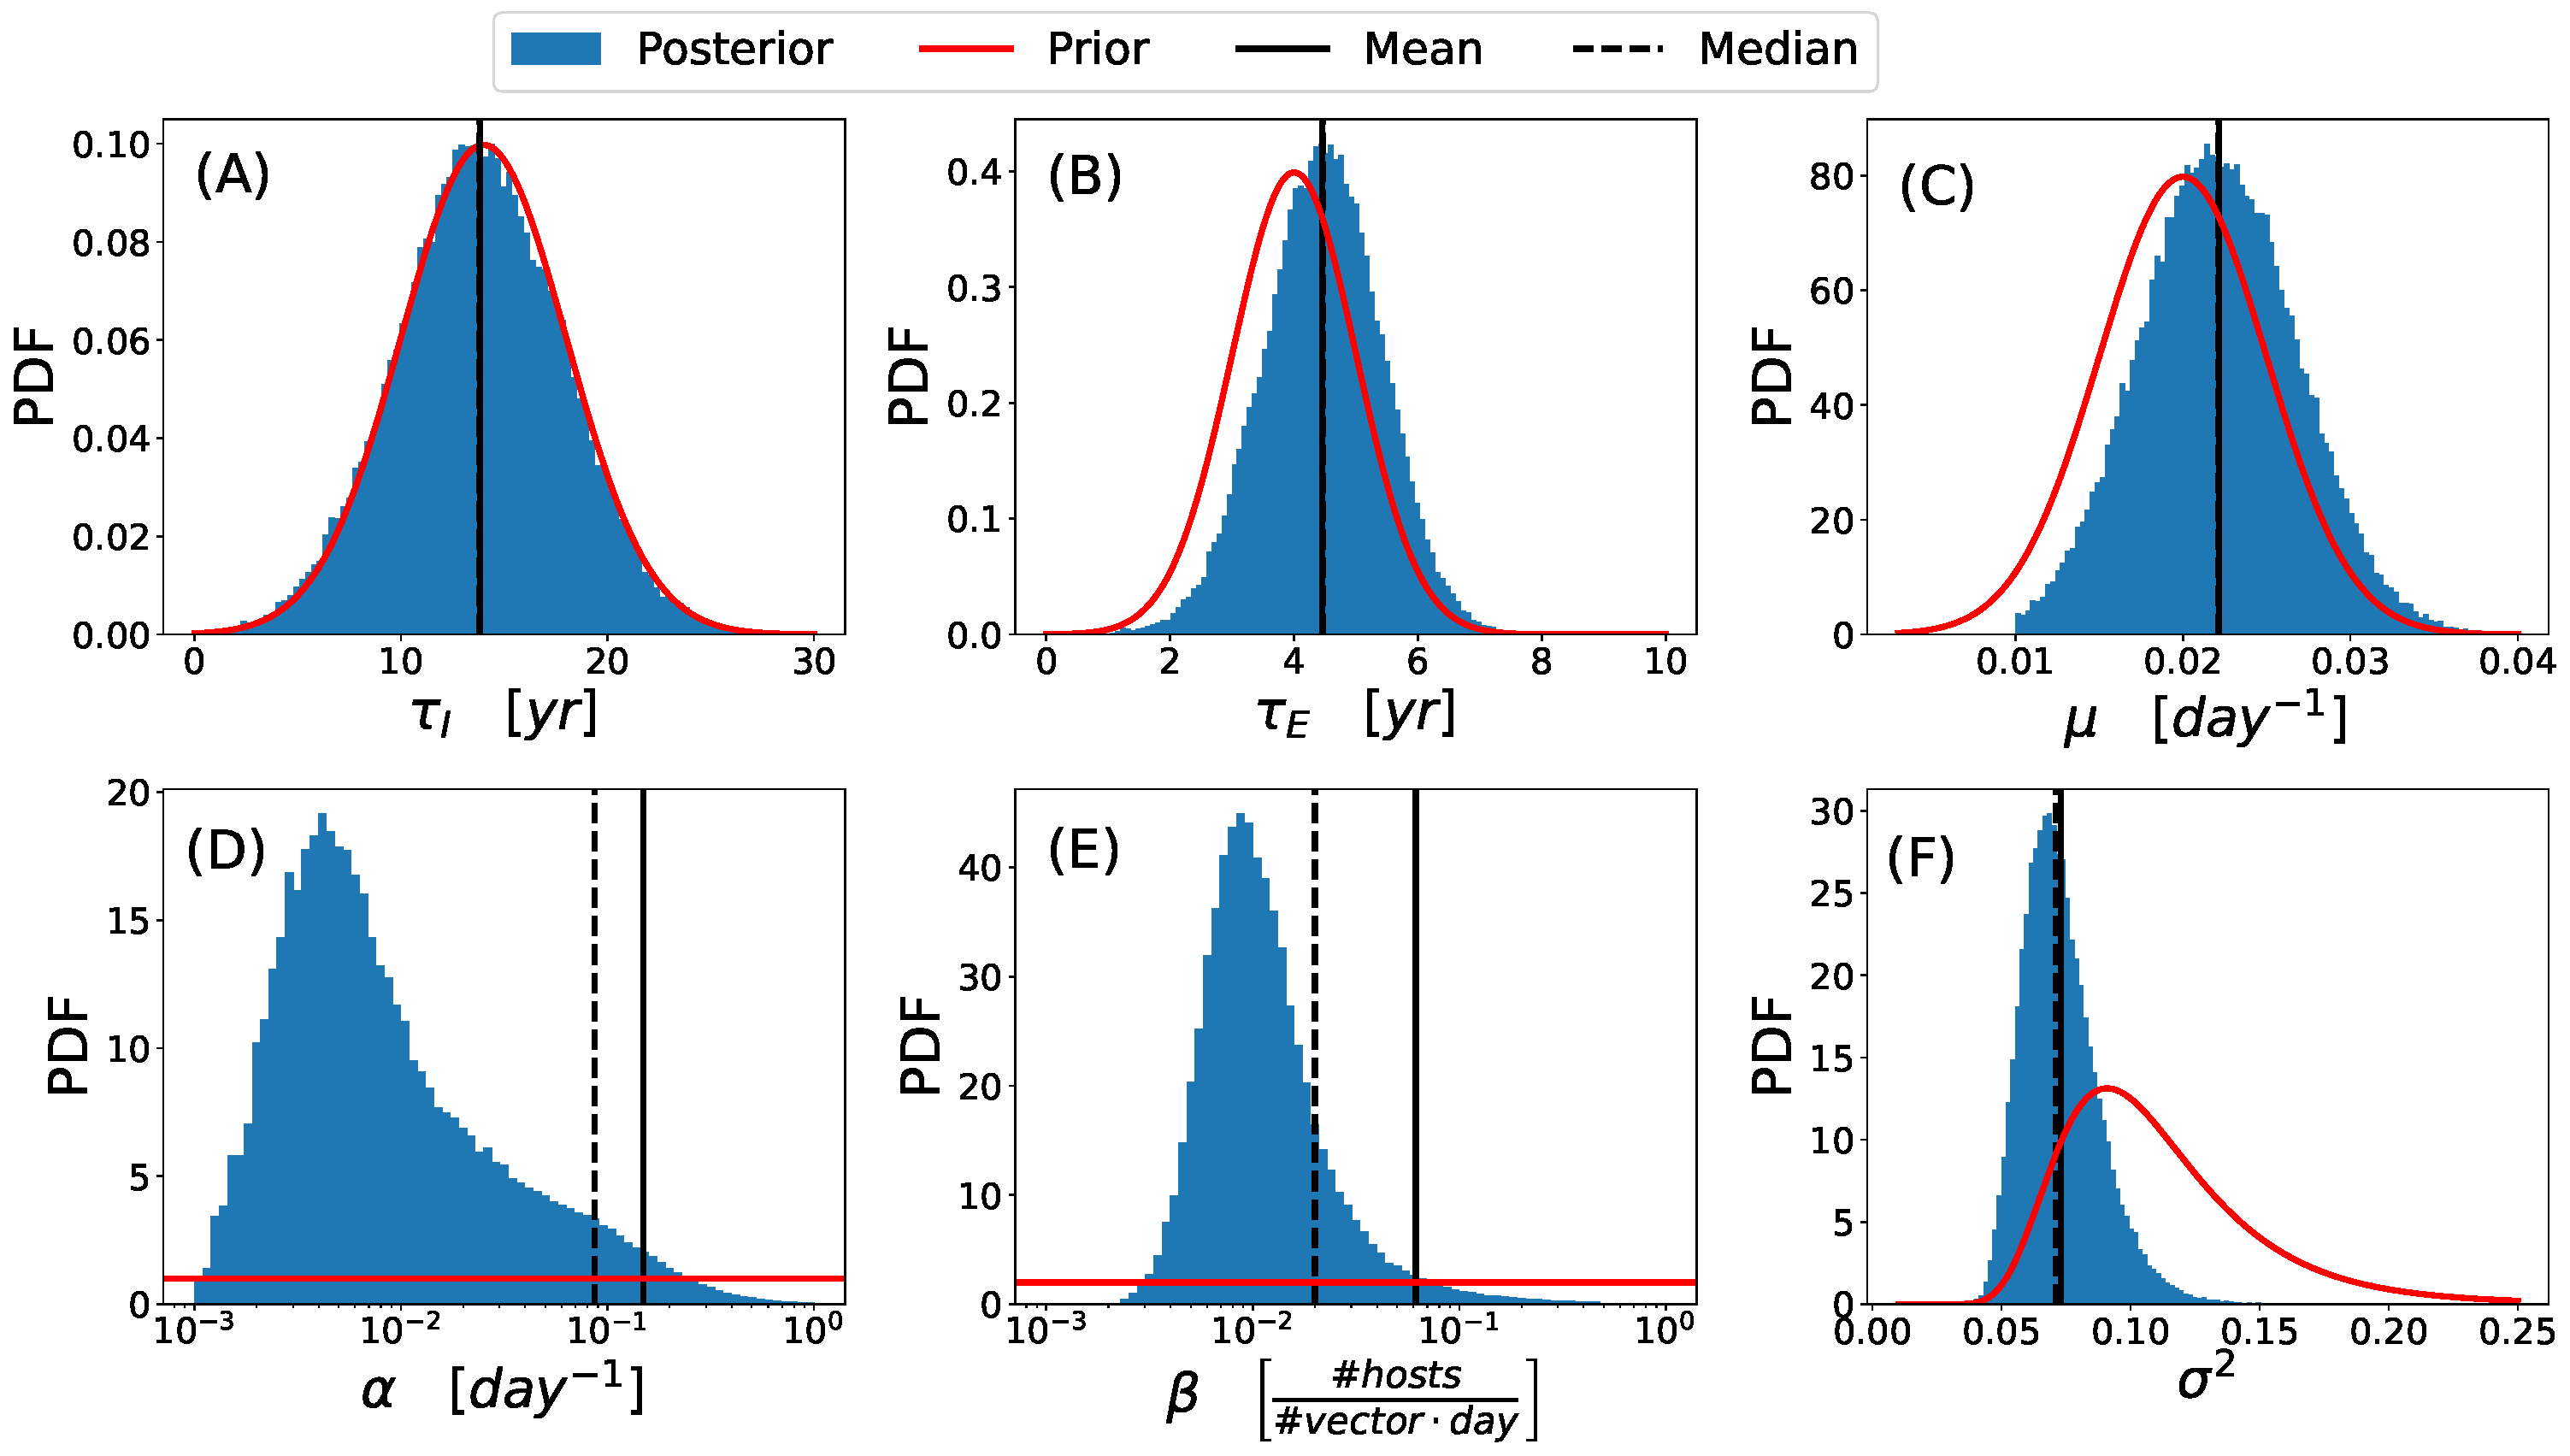
\includegraphics[width=0.9\textwidth]{Figures/Parameter_estimates_ALSD.pdf}
    \caption[Posterior and prior distributions of the model parameters for
        ALSD]{Posterior (blue histograms) and prior (red line) distributions
        of the model parameters for ALSD. Solid and dashed black lines
        correspond to
        the mean and median of the posterior distributions. (A) Host infectious
        period
        $\tau_I=1/\gamma$. (B) Host latent period $\tau_E=1/\kappa$.  (C)
        Vector
        removal rate $\mu$. (D) Vector infection rate $\alpha$. (E) Host
        infection rate
        $\beta$. (F) The variance of the field data $\sigma^2$.}
    \label{fig:parameter_estimates_ALSD}
\end{figure}

\begin{figure}[H]
    \centering
    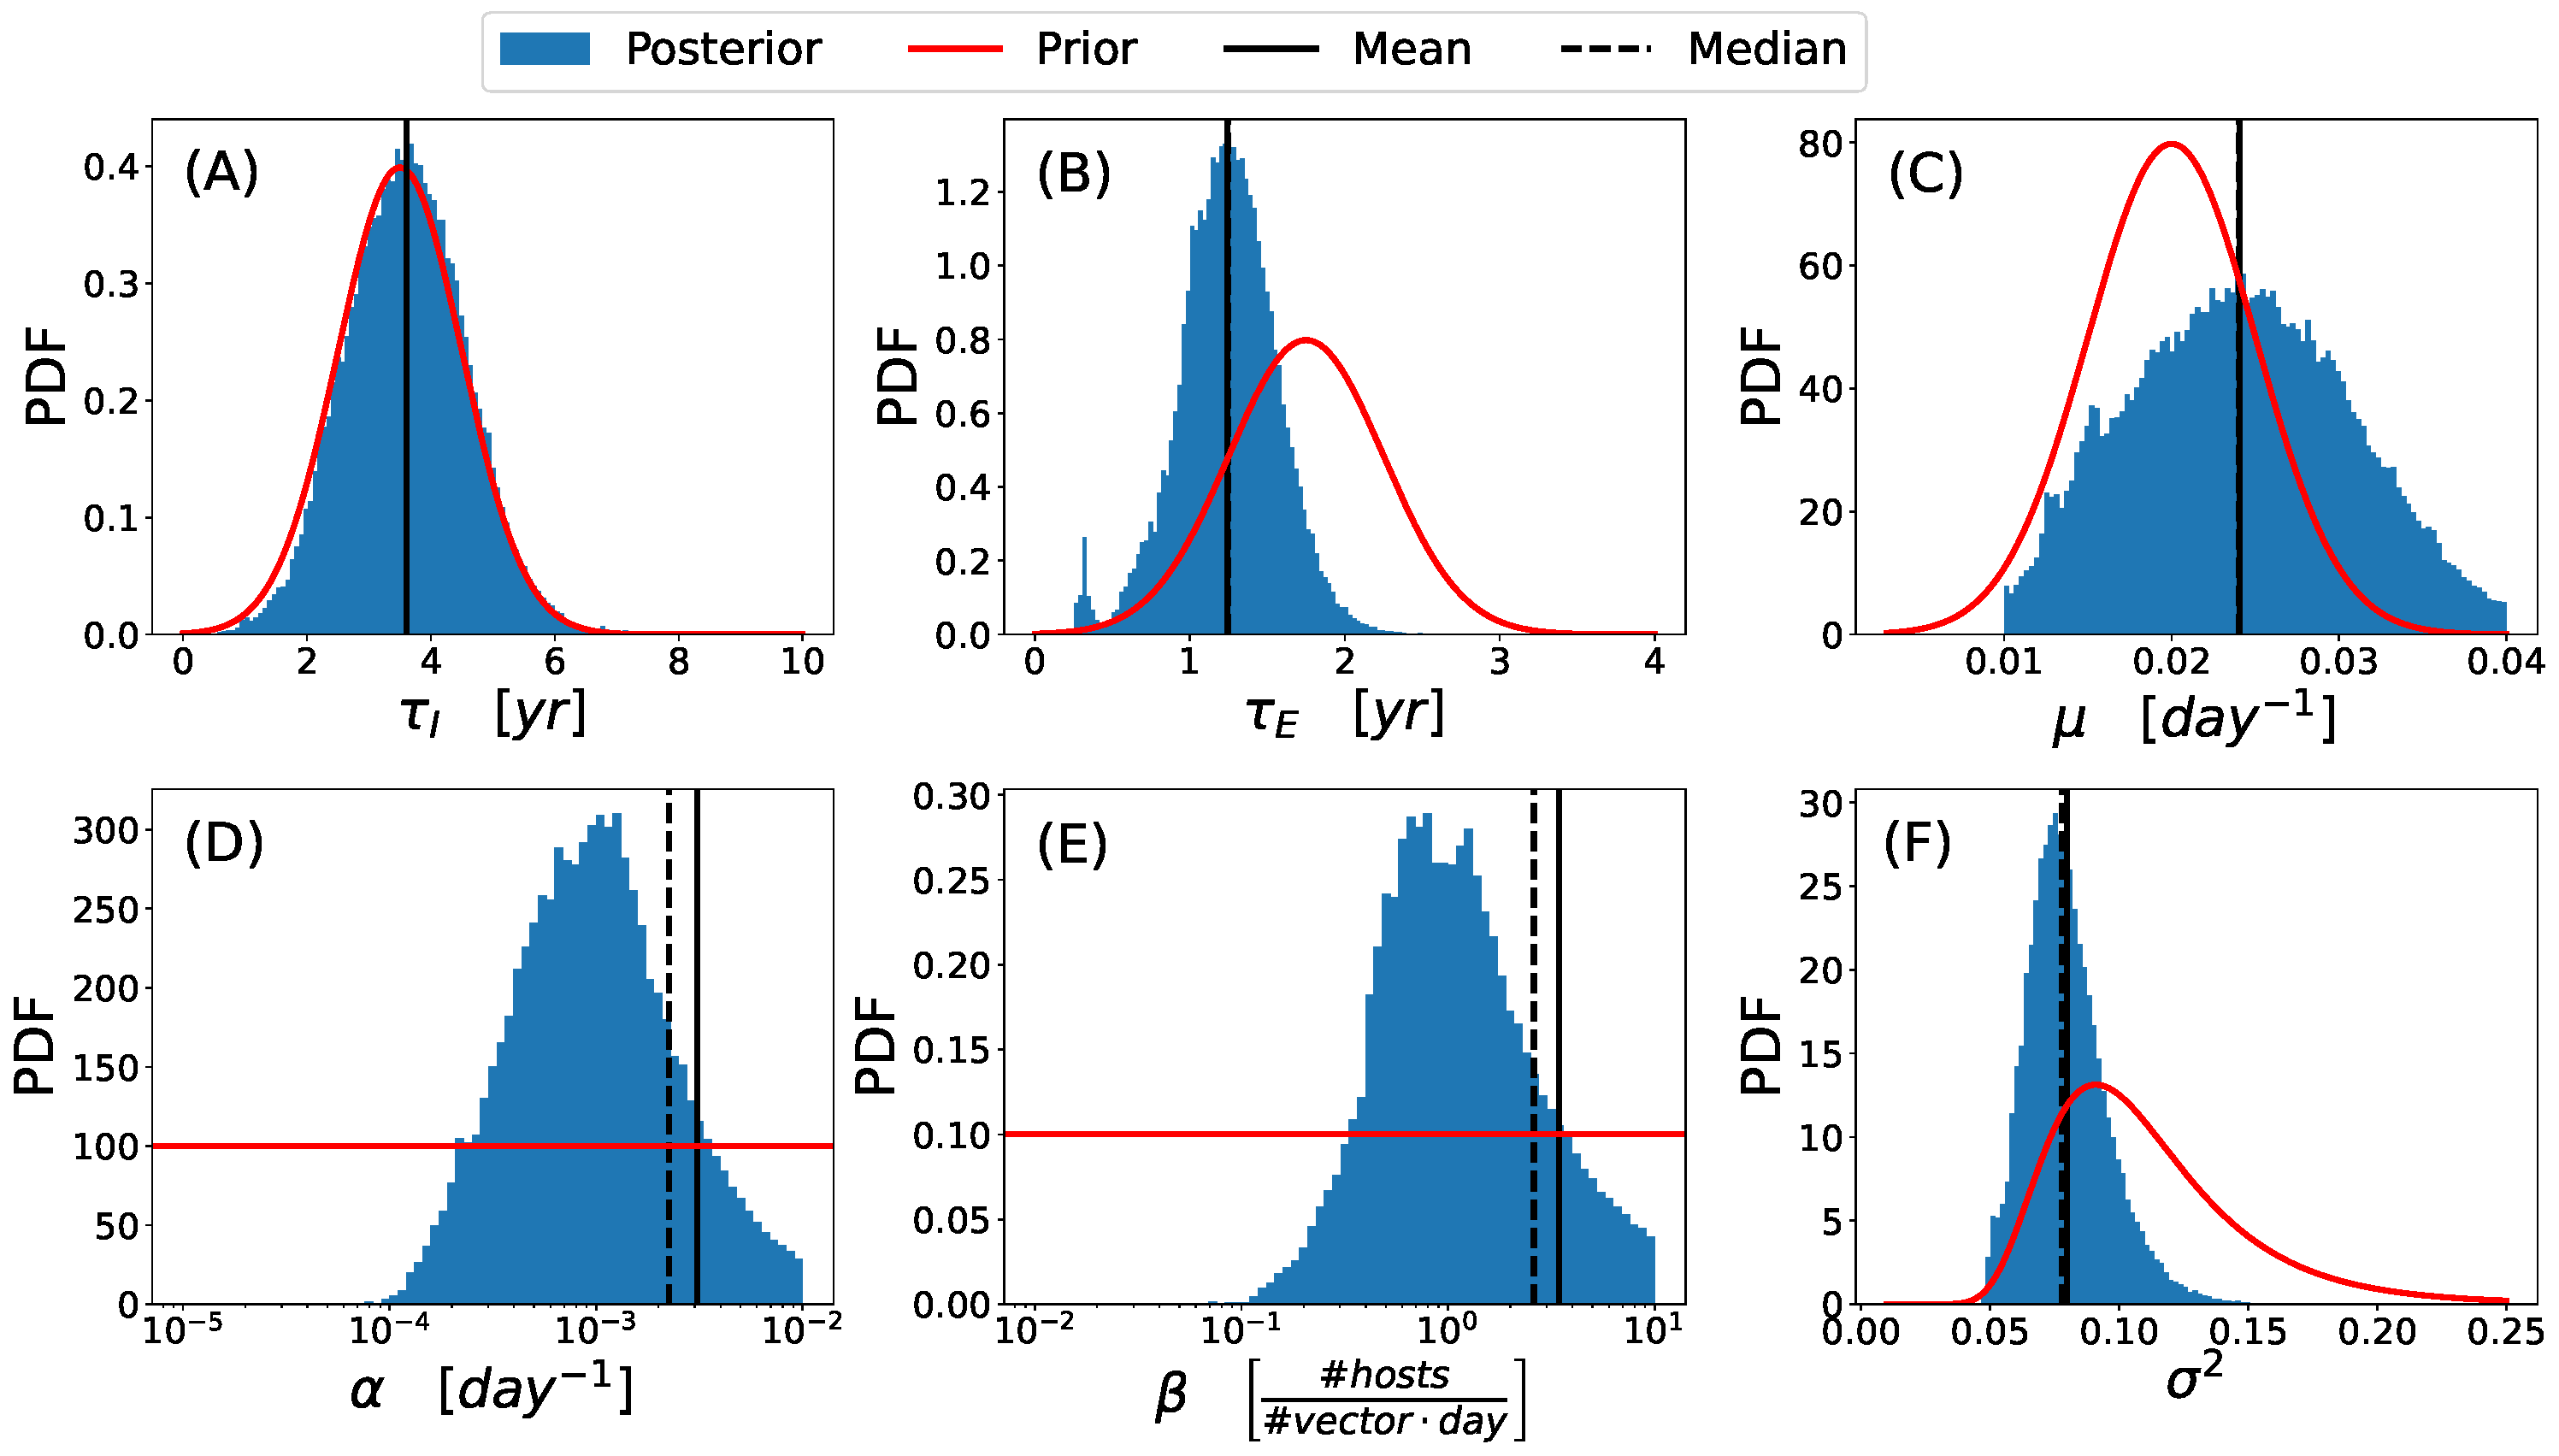
\includegraphics[width=0.9\textwidth]{Figures/Parameter_estimates_OQDS.pdf}
    \caption[Posterior and prior distributions of the model parameters for
        OQDS]{Posterior (blue histograms) and prior (red line) distributions
        of the model parameters for OQDS. Solid and dashed black lines
        correspond to
        the mean and median of the posterior distributions. (A) Host infectious
        period
        $\tau_I=1/\gamma$. (B) Host latent period $\tau_E=1/\kappa$. (C) Vector
        removal
        rate $\mu$. (D) Vector infection rate $\alpha$. (E) Host infection rate
        $\beta$. (F) Variance of the field data $\sigma^2$.}
    \label{fig:parameter_estimates_OQDS}
\end{figure}

Mean and median parameter estimates, i.e. the best-fit parameter values for
ALSD and OQDS, are summarized in
\cref{tab:parameter_estimates_ALSD,tab:parameter_estimates_OQDS}, respectively.
As already seen from the posterior distributions, the best-fit values for
$\tau_E$, $\tau_I$ and $\mu$ are close to the ones given by literature and
field data for both diseases. Conversely, $\alpha$ and $\beta$ are rather
uninformative, as their 95\% confidence intervals cover almost two orders of
magnitude. This again indicates that without some data about the evolution of
the vector states in time, $S_v(t)$ and $I_v(t)$, it is nearly impossible to
derive the proper values for these parameters.

\begin{table}[H]
    \centering
    \caption[Estimated parameters of the model for ALSD in Mallorca]{Estimated
        epidemiological
        parameters from Bayesian model
        fitting to the disease progression curve of ALSD in Mallorca.}
    \resizebox{\textwidth}{!}{
        \begin{tabular}{cccccc}
            \hline \hline
            \textbf{Parameter}      & \textbf{Definition}       &
            \textbf{Units}          &
            \textbf{Posterior Mean} & \textbf{Posterior Median} & \textbf{95\%
                C.I.}
            \\
            \hline
            $\tau_I$                & Host infectious period    & yr
                                    & $13.84$                   & $13.82$
                                    &
            $[7.12, 20.47]$
            \\
            $\tau_E$                & Host latent period        & yr
                                    & $4.46$                    & $4.47$
                                    & $[2.88,
                        5.99]$
            \\
            $\beta$                 & Host infection rate       &
            $\SI{}{\frac{\#host}{\#vector
            \cdot day}}$            & $0.062$                   & $0.02$
                                    & $[0.0061, 0.3013]$
            \\
            $\alpha$                & Vector infection rate     &
            $\SI{}{day^{-1}}$       & $0.15$                    &
            $0.086$                 & $[0.0047, 0.54]$
            \\
            $\mu$                   & Vector removal rate       &
            $\SI{}{day^{-1}}$       & $0.0222$                  &
            $0.0221$                & $[0.015, 0.030]$
            \\
            $R_0$                   & Basic reproductive number & -
                                    & 133                       & 25
                                    & -
            \\ \hline
            \hline
        \end{tabular}
    }
    \label{tab:parameter_estimates_ALSD}
\end{table}

\begin{table}[H]
    \centering
    \caption[Estimated parameters of the model for OQDS in Apulia]{Estimated
        epidemiological parameters from Bayesian model
        fitting to the disease progression curve of OQDS in Apulia.}
    \resizebox{\textwidth}{!}{%
        \begin{tabular}{cccccc}
            \hline \hline
            \textbf{Parameter}      & \textbf{Definition}       &
            \textbf{Units}          &
            \textbf{Posterior Mean} & \textbf{Posterior Median} & \textbf{95\%
                C.I.}
            \\
            \hline
            $\tau_I$                & Host infectious period    & yr
                                    & $3.61$                    & $3.60$
                                    & $[2.06,
                        5.20]$
            \\
            $\tau_E$                & Host latent period        & yr
                                    & $1.24$                    & $1.25$
                                    & $[0.70,
                        1.75]$
            \\
            $\beta$                 & Host infection rate       &
            $\SI{}{\frac{\#host}{\#vector
            \cdot day}}$            & $3.44$                    & $2.60$
                                    & $[0.55, 8.79]$
            \\
            $\alpha$                & Vector infection rate     &
            $\SI{}{day^{-1}}$       & $0.0031$                  &
            $0.0022$                & $[0.0005, 0.0084]$
            \\
            $\mu$                   & Vector removal rate       &
            $\SI{}{day^{-1}}$       & $0.0240$                  &
            $0.0240$                & $[0.014, 0.035]$
            \\
            $R_0$                   & Basic reproductive number & -
                                    & 33                        & 21
                                    & -
            \\ \hline
            \hline
        \end{tabular}
    }
    \label{tab:parameter_estimates_OQDS}
\end{table}

Overall, the data falls within the 99\% confidence limits of the fitted
model for both the ALSD and OQDS outbreaks (\cref{fig:best_fit_model} (B,D)).
We
also computed the instantaneous reproductive number, $R_0(t)$, by using
\cref{eq:R0} with $S_H(t)$ instead of only $S_H(0)$ along the simulation.
Noteworthy, $R_0(t)=1$ coincides with the stopping of new infections being
produced, i.e. the number of exposed hosts does not increase
(\cref{fig:best_fit_model} (A,C)). This supports our approximate method for
computing the reproductive number for Xf diseases (\cref{app:R0},
\cref{eq:R0}). Due to the different time scales of both epidemics
($\tau_I^{ALSD}+\tau_E^{ALSD} > \tau_I^{OQDS}+\tau_E^{OQDS}$), the OQDS
outbreak dies out earlier than the one for ALSD.

We notice that for ALSD a large proportion of the vector population gets
infected every year (\cref{fig:best_fit_model} (A)), while a very small
proportion is needed in OQDS to produce a lethal outbreak
(\cref{fig:best_fit_model} (C)). However, this last statement is rather
unrealistic, as around 50\% of the vectors that are captured in Apulia are
indeed infected by Xf \cite{Cavalieri2019,cornara2017transmission}. Thus, the
evolution of the infected vector population should be qualitatively similar to
that obtained for ALSD (\cref{fig:best_fit_model} (C)). As previously
explained,
different suitable combinations of $\alpha$ and $\beta$ parameters should give
rise to similar progression curves for the hosts while different ones for the
vectors, but the realistic values for these parameters cannot be obtained from
the Bayesian fit due to the lack of data of the vector states, $S_v(t)$,
$I_v(t)$.

\begin{figure}[H]
    \centering
    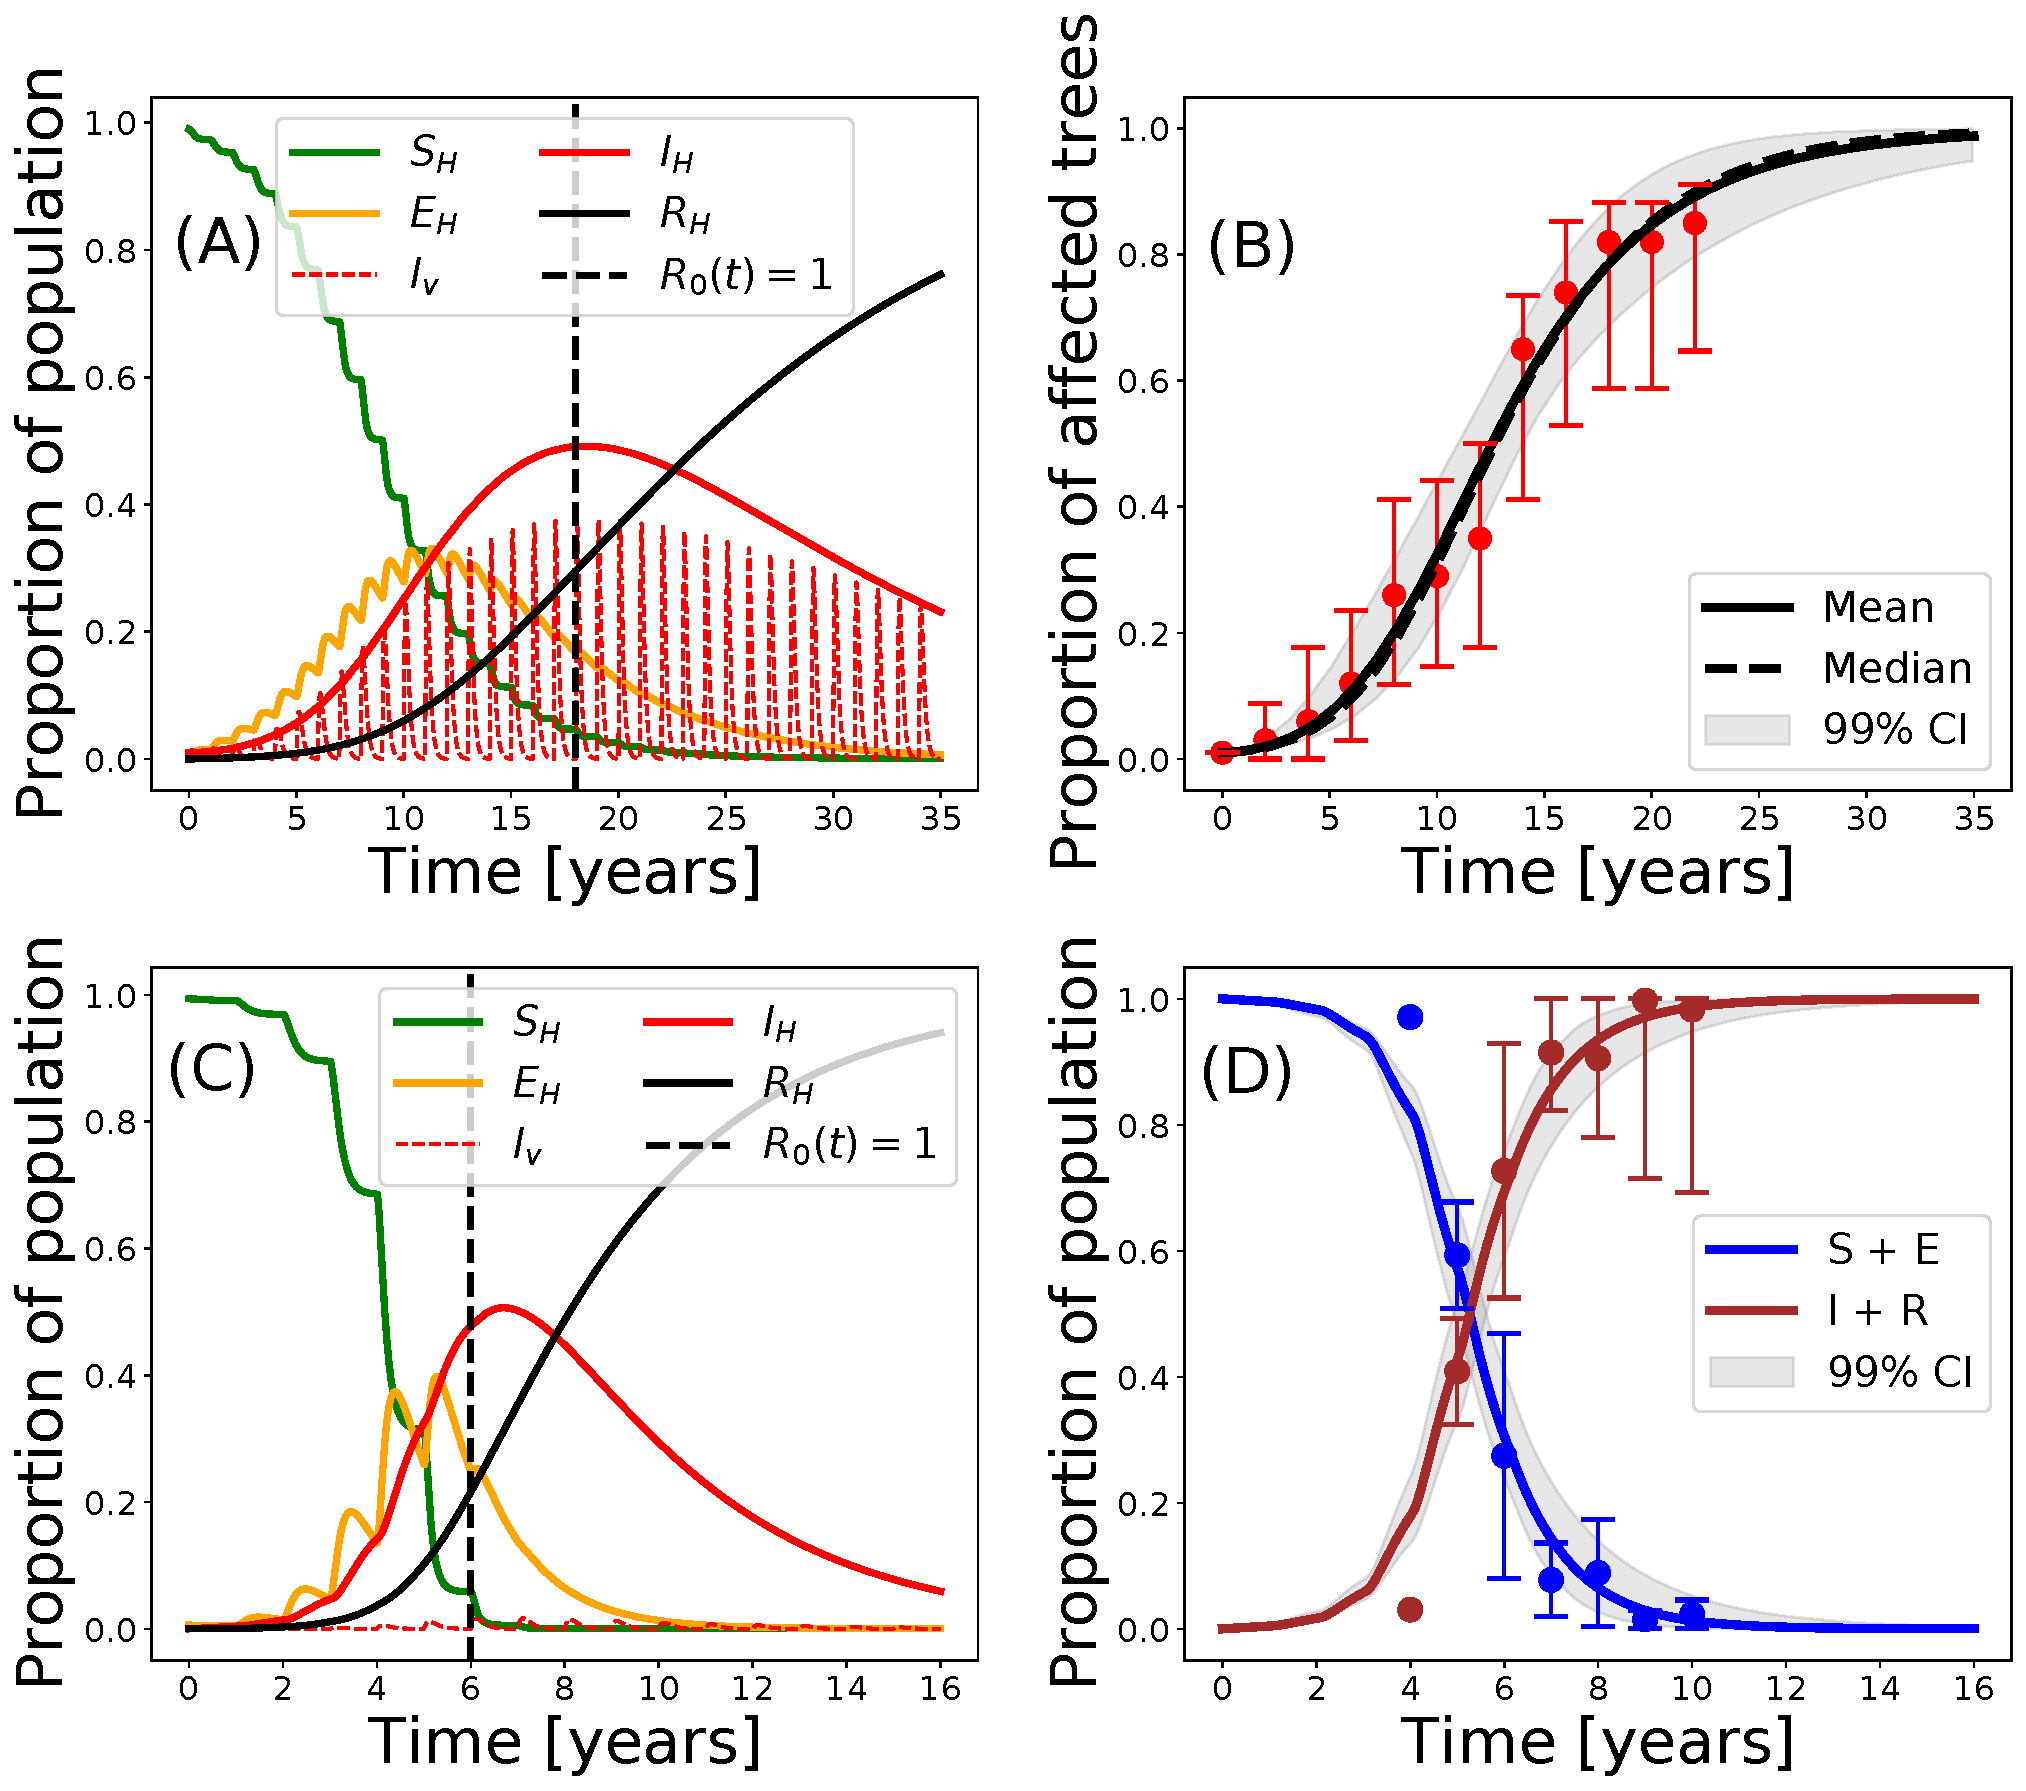
\includegraphics[width=0.9\textwidth]{Figures/BayesianInference.pdf}
    \caption[Best-fit model to the field data for ALSD and OQDS]{(A) Simulation
        of the model with the best-fit parameters for
        ALSD. (B) Model fit to field data by means of the mean and median
        values of the
        posterior distributions of the parameters for ALSD. (C) Simulation of
        the model
        with the best-fit parameters for OQDS. (D) Model fit to field data by
        means of
        the mean and median values of the posterior distributions of the
        parameters for
        OQDS. The gray-shaded area corresponds to the 99\% confidence interval.
        The
        error bars for the field data correspond to their 95\% confidence
        interval
        obtained with a bootstrapping technique.}
    \label{fig:best_fit_model}
\end{figure}

Nevertheless, by manually exploring other values for $\alpha$ and $\beta$
parameters, we can obtain a more biologically plausible scenario for the OQDS
that is still able to fit the available data for the hosts.
\cref{fig:best_fit_model_OQDS} (A) shows a simulation of the model with
previously inferred best-fit median parameters for OQDS. By changing the values
of $\alpha$ and $\beta$, we obtain a more realistic scenario, i.e. around a
50\% of the vector population getting infected during the outbreak
(\cref{fig:best_fit_model_OQDS} (B)) \cite{Cavalieri2019,
    cornara2017transmission}. Noteworthy, the $\beta$ value obtained in this
way
is almost identical to the transmission rate recently reported by
\cite{Bodino2021} for OQDS. This change in the transmission parameters only
affects the progression curve of the infected vector population, being the
progression of the host compartments practically unchanged
(\cref{fig:best_fit_model_OQDS} (C)). Anyway, both sets of parameter values for
$\alpha$ and $\beta$ can properly fit the field data, corresponding exclusively
to the	host population (\cref{fig:best_fit_model_OQDS} (D)).

The model adjusted to the progression curves of both diseases indicates
that the transmission rate $\alpha$ must be greater than $\beta$ when the
proportion of infected vectors is relatively high ($>30\%$). We checked if the
relation between $\alpha$ and $\beta$ held when changing the assumed
$N_v(0)=N_H/2$, obtaining that it kept approximately the same for very
different values of the initial vector population.

\begin{figure}[H]
    \centering

    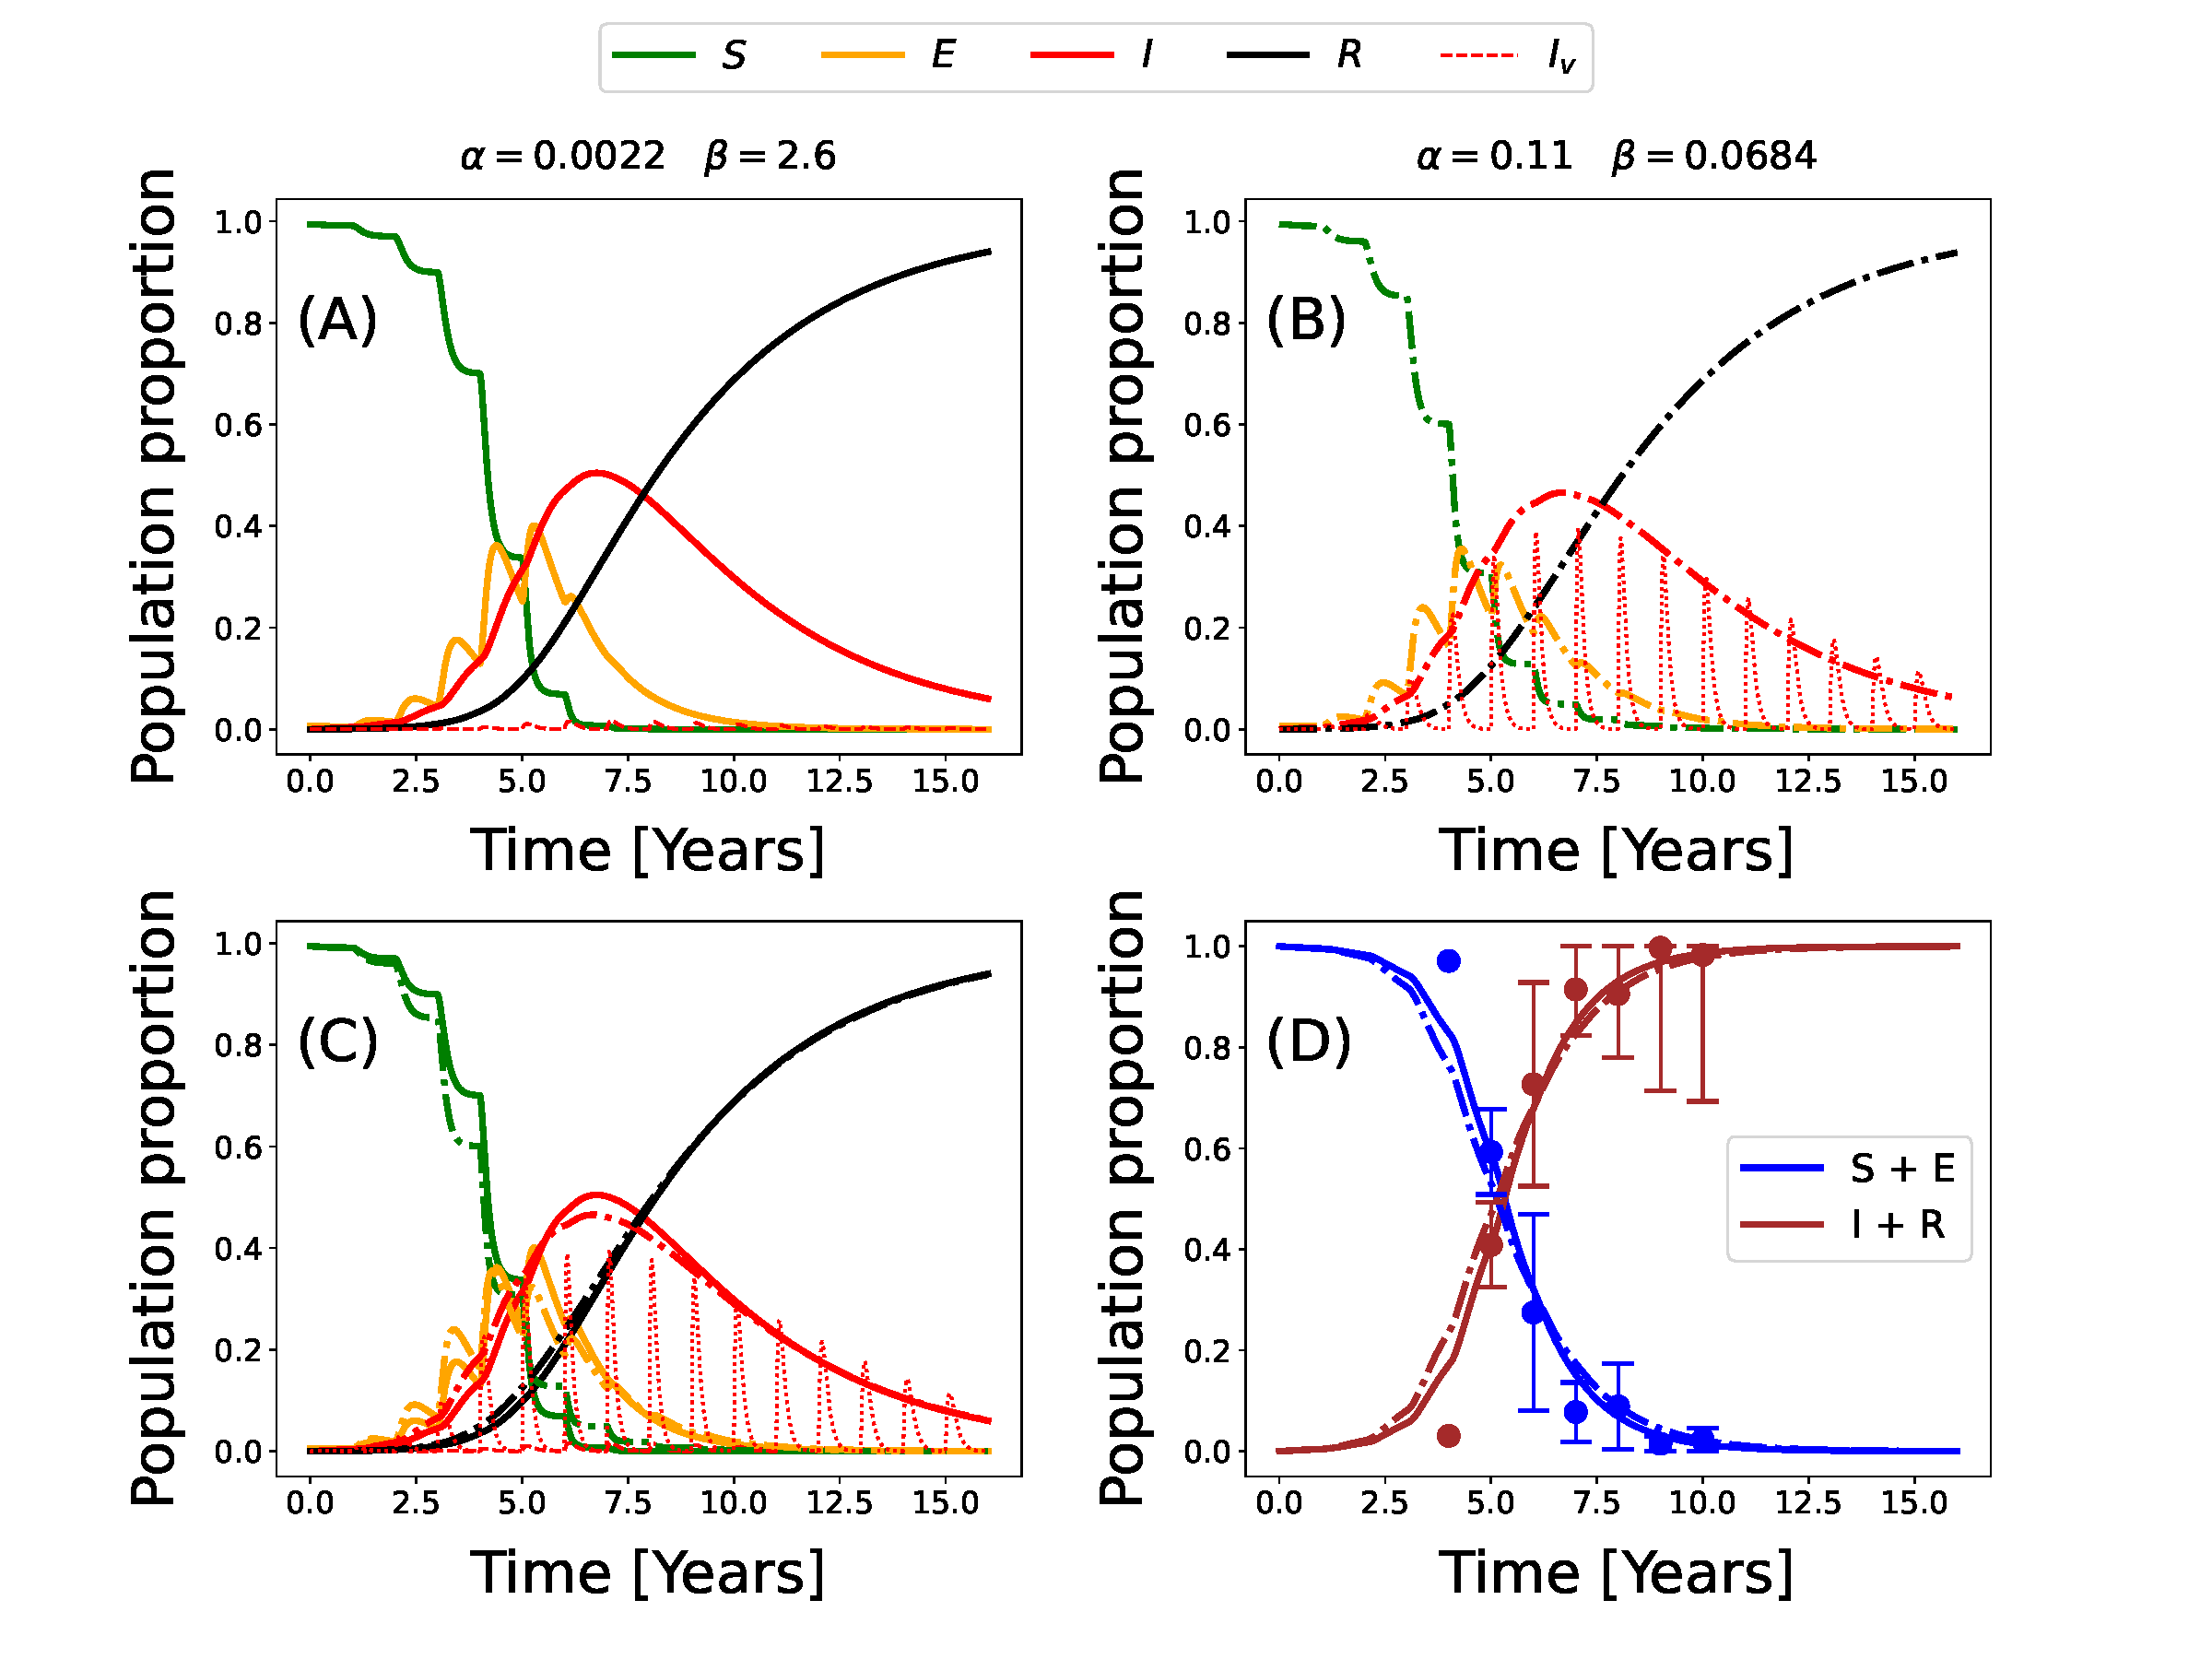
\includegraphics[width=\textwidth]{Figures/OQDS_different_vector_curves_same_host_curve.pdf}
    \caption[Comparison of the model fit to the data for OQDS with different
        transmission rates]{(A) Simulation of the model with the original
        best-fit
        parameters for OQDS. (B) Simulation of the model with the original
        best-fit
        parameters for OQDS but with different $\alpha$, $\beta$ values. (C)
        Comparison
        of the progression curves. Note that the curves for the hosts are very
        similar
        while the curve for the infected vector population is very different.
        (D)
        Comparison of the model fit to the data with both simulations. Solid
        lines
        correspond to results with the original best-fit parameters while
        dash-dot
        lines correspond to the results of the more realistic scenario with
        different
        $\alpha$ and $\beta$.}
    \label{fig:best_fit_model_OQDS}
\end{figure}

\subsection{Global Sensitivity Analysis}

We computed the sensitivity indices for the model parameters with respect
to the more relevant quantities of interest, namely, the time at which the
number of infectious hosts is maximal, $t_{\textrm{peak}}$, the maximum number
of infectious hosts, $I_{\textrm{peak}}$ and the final number of dead hosts,
$R_\infty$. The results were obtained exploring the parameter space constrained
to the intervals $\{\beta\in(0.001, 0.1), \ \tau_E\in(3,7), \ \tau_I\in(5,25),
    \ \alpha\in(0.001, 1), \ \mu\in(0.01, 0.04)\}$ using $10^4$ Quasi-Monte
Carlo
samples and are summarized in \cref{fig:GSA}.

Parameters $\alpha, \ \beta$ and $\mu$ are the most influential with regard
to the time at which the infectious host population peaks, $t_{peak}$, the
magnitude of the peak, $I_{peak}$, and the final number of dead hosts,
$R_{\infty}$. The total output variance (total order indices) cannot be
explained by the variances of the parameters alone (first order indices)
(\cref{fig:GSA}). Therefore, higher-order interactions among the parameters
importantly affect the sensitivity of the quantities under study. Indeed, the
contribution to the total output variance of $\gamma$ and $\kappa$ for
$t_{peak}$ and $R_{\infty}$ come notably from higher-order interactions. This
can be checked in panels (B,C,F) of \cref{fig:GSA}, in which the contribution
to the output variance from interactions between pairs of parameters (second
order indices) is represented. Interactions among the parameters contribute to
increasing the output variance with respect to $t_{peak}$ and $I_{peak}$, while
the effect is more heterogeneous in the case of $R_{\infty}$. In particular,
the interactions between $\alpha-\beta$ and $\alpha-\mu$ produce the main
contributions to the increase of output variance in all cases, while
$\kappa-\beta$, $\kappa-\alpha$ and $\kappa-\mu$ interactions decrease the
output variance.

\begin{figure}[H]
    \centering
    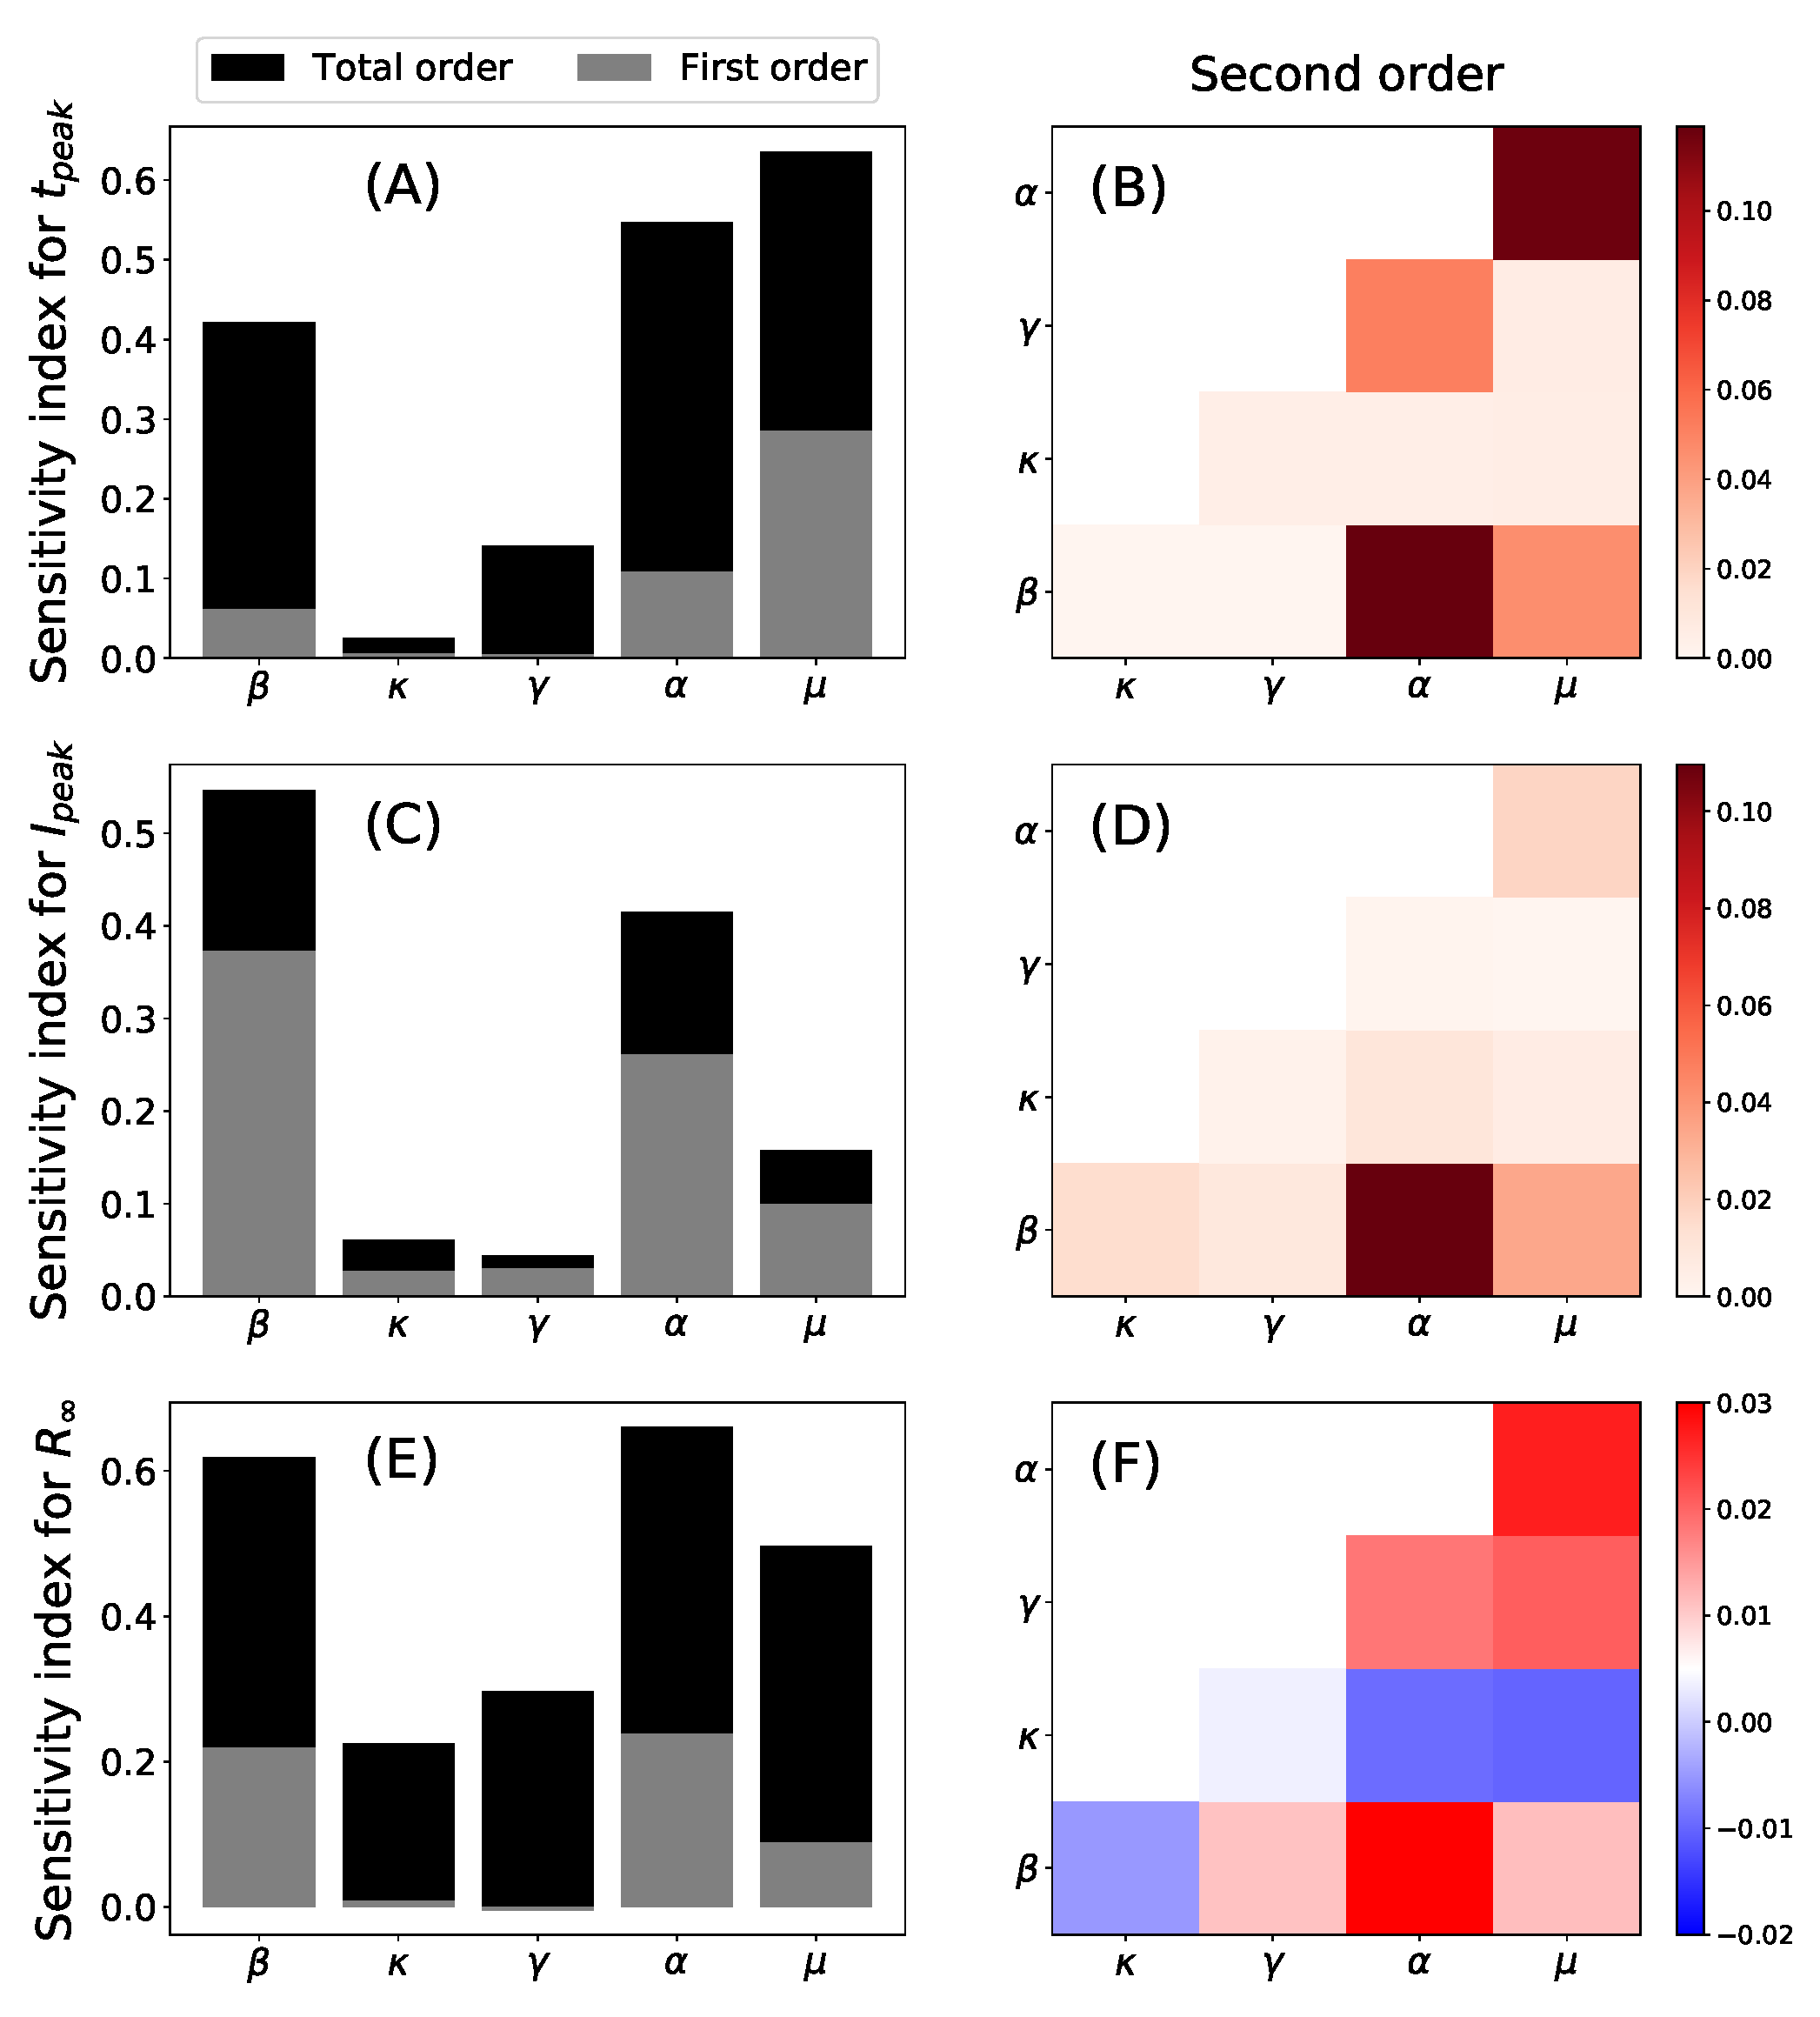
\includegraphics[width=0.75\textwidth]{Figures/GSA.pdf}
    \caption[Global Sensitivity Analysis of the model]{Global Sensitivity
        Analysis of the model parameters performed
        with the Sobol method with respect to the time at which the infectious
        population peaks, $t_{peak}$ (A-B), the magnitude of this peak,
        $I_{peak}$
        (C-D) and the final number of dead hosts, $R_{\infty}$ (E-F). The left
        column
        (A,C,E) shows the total and first-order indices and the right column
        (B,D,F)
        shows the second-order indices.}
    \label{fig:GSA}
\end{figure}

\subsection{Epidemic control through vector management}

The sensitivity analysis clearly indicates that acting on $\alpha,\beta$
and $\mu$ is the best strategy to lower disease incidence and mortality.
However, controlling transmission rates is cumbersome so a different control
strategy based only on vector control is considered in this section. In our
model, there are two ways of implementing vector-population control: (i)
decreasing the typical time, $1/\mu$, that vectors spend between crops each
year by some mechanism (thus increasing $\mu$) and (ii) reducing the initial
number of vectors that invade crops each year (e.g. lowering $N_v(0)$ via egg
or nymph control \cite{Lago2022}).

We analyzed the effect of vector management by simulating epidemic
outbreaks using different values of $\mu$ and $N_v(0)$, and keeping the rest of
parameters as fitted for both ALSD and OQDS outbreaks
(\cref{fig:control_strategy}). In both epidemics, decreasing the presence time
as well as the number of vectors contribute to controlling the epidemic by
lowering $R_0$ and, consequently, the final size of the epidemic, $R_{\infty}$.
Furthermore, we observe that decreasing vector presence is more efficient than
decreasing its annual initial population, i.e. we further reduce $R_{\infty}$,
the final size of the epidemic, by applying a similar reduction in the
residence time $1/\mu$. This could also be anticipated as $R_0$ depends
quadratically on $1/\mu$ while only linearly on $N_v(0)$ (\cref{eq:R0}).
However, the minimal intervention strategy, starting from the current situation
in the $(1/\tau,N_v(0))$ parameter space that yields an absolute control of the
epidemic, $R_0<1$, involves a mixed strategy of lowering both $1/\mu$ and
$N_v(0)$.

\begin{figure}[H]
    \centering
    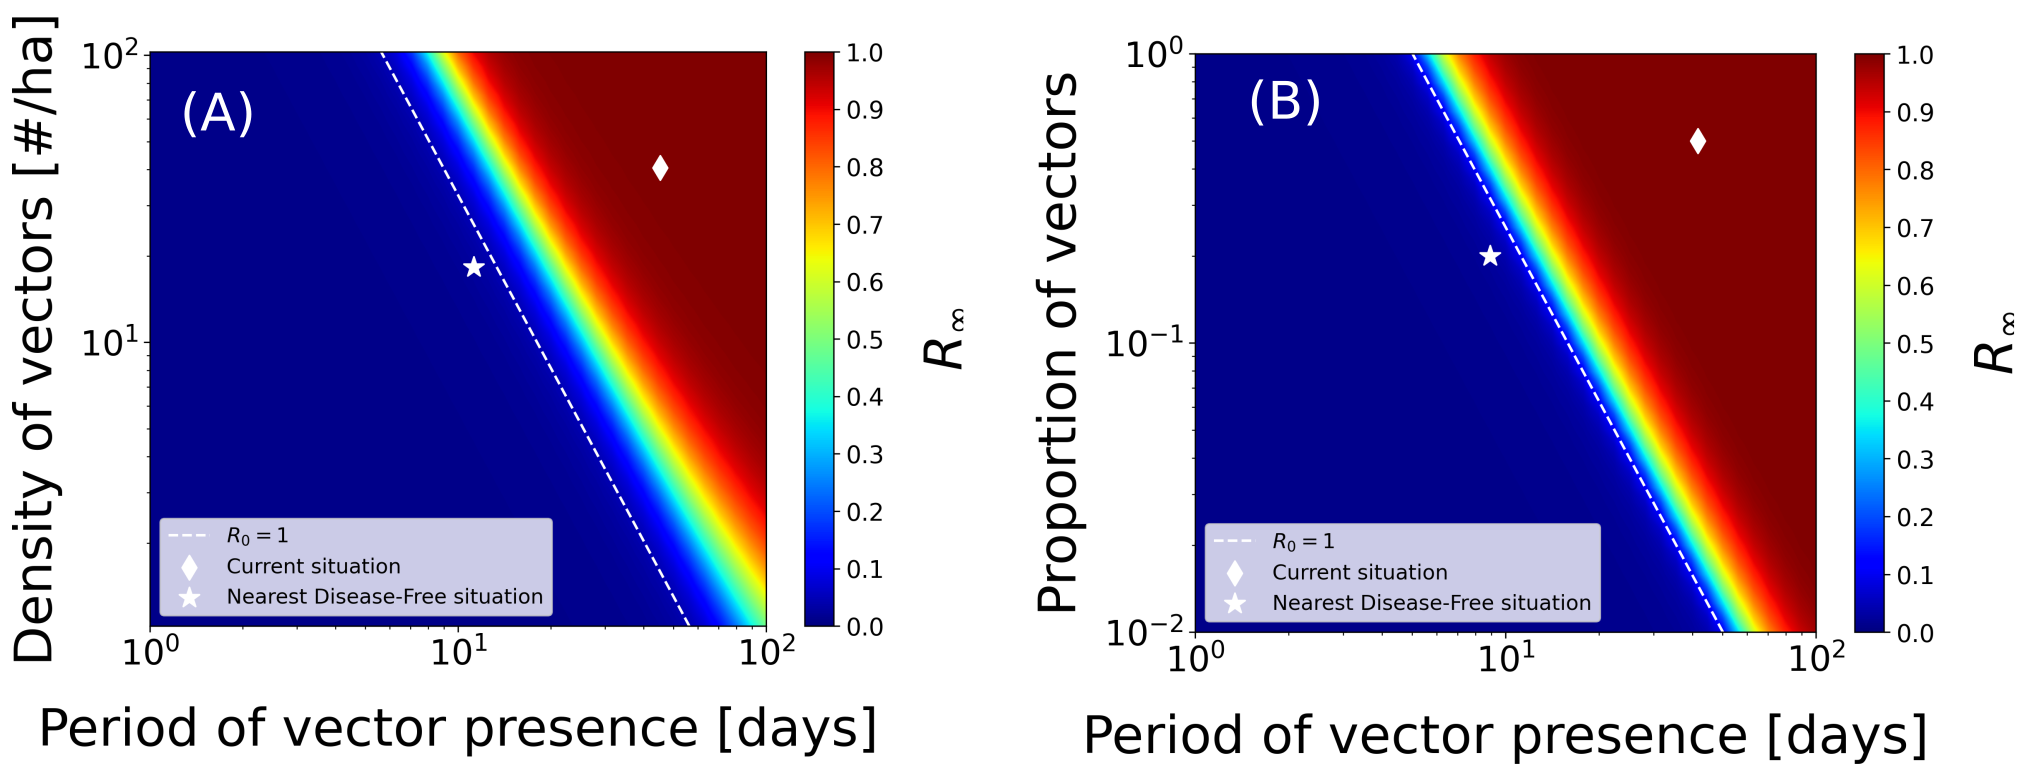
\includegraphics[width=\textwidth]{Figures/Control_strategy.png}
    \caption[Epidemic control through vector management for ALSD in Mallorca
        and
        OQDS in Apulia]{Epidemic control through vector management for ALSD in
        Mallorca (A) and OQDS in Apulia (B). The white shaded line denotes
        $R_0=1$, the
        white diamond corresponds to the parameter values of the fitted model.
        The
        white star is the closest disease-free state to the current situation
        in this
        representation.}
    \label{fig:control_strategy}
\end{figure}

\section{Discussion}

In this work, we have developed a deterministic continuous-time
compartmental model for \textit{Xylella fastidiosa} vector-borne diseases in
Europe. The model attempts to characterize the main biotic processes that lead
to the development of epidemics, including the seasonal dynamics of the main
vector, \textit{P. spumarius}. We show how the model is sufficiently general to
represent with some accuracy the parameters that determine the ALSD in Mallorca
(Spain) and the OQDS in Apulia (Italy), both transmitted by \textit{P.
    spumarius}. To our best knowledge, this is the first mathematical model
describing Xf epidemics that considers the temporal pattern of vector abundance
observed in field data, faithfully representing the known biological
information about the pathosystem. It includes a dynamic approximation of the
non-stationary populations of \textit{P. spumarius}, mathematically represented
by a sporadic source term through which vectors are born every year, and an
exponential decay term. Due to the non-stationarity of the vector dynamics,
$R_0$ in the model cannot be computed with standard methods such as the Next
Generation Matrix \cite{Diekmann2010}. To circumvent this problem, we applied
an approximate method to compute it as previously proposed by
\cite{GimenezRomero2022_PRE}. We show that this approximate $R_0$ correctly
characterizes the epidemic, further validating the method proposed by
\cite{GimenezRomero2022_PRE}.

Nonlinear mathematical models of disease transmission enhance our
understanding of the different mechanisms operating in an epidemic, especially
compared with correlative or machine learning methods, often very useful in
practice but offering very little understanding. A key aspect to render these
models useful is the determination of the parameters from available data. If
this step can be properly performed, these models become very predictive and
especially helpful to design disease control strategies. However, an
appropriate calibration of the model relies on access to good-quality field
data, which is often the bottleneck for the application of this kind of models.
In the present study, the parameters have been obtained using a Bayesian
inference framework, which relies on probability distributions rather than
point-like measures. This way, mean or median values can be considered together
with their confidence intervals able to characterize the robustness of the
obtained parameters. In general, we obtained different values of the parameters
for the ALSD and OQDS outbreaks in Mallorca and Apulia, respectively. The
fitted values, however, are in good agreement with previous field-based
measures for each disease while the differences observed between both outbreaks
may reflect differences between the Xf subspecies and crops involved (deciduous
vs. evergreen).

One of the conclusions of the study is that the available data for both
diseases is not enough to obtain robust estimates for all of the model
parameters. The lack of data about the vector population compartments yields
many possible values for the parameters that regulate transmission, $\alpha$
and $\beta$, provided that the progression of the host compartments correctly
fits the field data. In other words, very infectious vectors (high $\beta$)
that hardly ever get infected (low $\alpha$) can produce a similar outbreak
within the host population to that produced by very low infectious vectors (low
$\beta$) that get infected very often (high $\alpha$). The great difference in
these situations would be that, in the former, the infected vector population
would be very low, while in the latter, it would be quite high. This is a
manifestation of parameter unidentifiability from the fit
\cite{Chowel2017,Roosa2019}, which stresses the importance of transmission
and calls for detailed measurements of the vector population, and not just of
the hosts. Furthermore, to compare transmission rates between different
diseases caused by Xf (e.g. $\beta$, $\alpha$), it is necessary to know the
vector-host population ratio of the pathosystem ($N_v/N_H$), since $\beta$ is
expressed as a number of hosts per vectors per day. Although, in general,
populations of \textit{P. spumarius} in the canopy of olive trees are much
larger than those found in the almond trees of the Balearic Islands during the
months of July and August \cite{Lopez2021},
our work is based on data from studies in which information of the vector
populations is not provided. Without this information, therefore, conclusive
results regarding transmission cannot be obtained.

In any case, our model shows that the vector-to-plant transmission process,
mediated by $\beta$, is somehow different from that from the plant-to-vector
one, mediated by $\alpha$. In essence, $\beta$ must be smaller than $\alpha$ in
order to reproduce the observed outbreaks and have a sufficiently large vector
population getting infectious, being this fact independent of the particular
choice of $N_v(0)/N_H$. This heterogeneity can be caused by several factors:
differences in the efficiency of plant-to-vector transmission with respect to
vector-to-plant transmission, differences in contact rates, i.e. susceptible
vectors contact trees at a different rate than infected vectors; vector feeding
preferences, i.e. differences in the probability of contacting a susceptible
host compared to an infectious host, etc. Indeed, our mathematical model
assumes constant contact rates with no preferences over any host state, so that
under these assumptions, it indicates that the probability of effectively
transmitting the pathogen from plant to vector is greater than from vector to
plant. However, this interpretation is subject to this particular assumption,
so that to fully disentangle this question experimental work in form of
transmission assays should be performed. Furthermore, we found that the timing
and magnitude of the infectious host peak and the final number of dead hosts
are mostly controlled by the vector-to-plant transmission rate, $\beta$, the
plant-to-vector transmission rate, $\alpha$ and the vector removal rate $\mu$.
Because these parameters are strongly related to the vector, the analysis makes
clear that enhancing the knowledge about the vector, as well as obtaining
precise data, is crucial to improve the modeling of Xf diseases and pose
important questions to be solved in specifically designed experiments.

The fact that the most influential parameters of the model are those
related to the vector can be used to design appropriate disease control
strategies. Because acting on transmission rates is rather cumbersome, we argue
that control strategies should focus on reducing the vector population in crop
fields. In our model, this depends on two parameters, $\mu$, the rate at which
vectors die (or move to herbaceous vegetation and other non-host trees or exit
the field) and $N_v(0)$, the number of newborns susceptible vectors every year
(assumed constant in this study). Our results show that a mixed strategy acting
on both parameters is optimal to lower disease prevalence and, eventually,
eradicate the disease. Interestingly, we also show that acting on the vector
removal $\mu$ is more effective than controlling the newborn vector population
$N_v(0)$. In fact, most control strategies carried out in practice for Xf
diseases focus on the latter factor, reducing $N_v(0)$ via egg or nymph control
\cite{Cornara2018, lopez2022mechanical, Lago2022}. However, our results
indicate that alternative strategies based on increasing the removal (or
dispersal) rate of vectors should be explored. Furthermore, the evolution of
the population compartments of the hosts and vectors provides relevant
information on the epidemiology of both diseases. In both cases, the newly
defined basic reproductive number that accounts for a decaying vector
population is very predictive of the moment in which new infections are not
produced anymore, coinciding approximately with the peak of infectious hosts.
Therefore, any intervention with control measures after this peak would have
marginal effects on future disease progression.

Our mathematical model is still rather simple, implementing only a few
relevant epidemic processes in contrast to the high complexity of the
pathogen-vector-host interactions occurring in plant epidemics. Indeed, the
model itself raises some questions about these interactions, for example,
whether or not contact rates are homogeneous. Another simplification of the
model is the fact that the spatial constraints and the intrinsic stochasticity
of the transmission processes are neglected. A straightforward extension of the
model would be to include a specific spatial setting and implement the explicit
motion of the vector within a stochastic framework, such as Individual Based
Models \cite{Grimm2005}. With this, the effectiveness of current and further
control strategies could be tested and improved controlling for the motion of
the vector. For instance, the control strategy based on the removal of
symptomatic trees together with their surrounding trees at a given distance
could be implemented in the model, evaluate the current effectiveness according
to the present protocols and even provide improved parameters to be implemented
in the field. Of course, implementing a model in which the spatial degrees of
freedom are explicitly represented would require access to further information
about vector mobility and spatially resolved data to confront the model, which
is not currently available.

Mathematical models tested against experimental data increase our understanding
of the system under study. They also help to identify critical
parameters that require better prior information to adjust functions relating
to different variables and make the model predictions more accurate to suggest
and test control strategies \cite{cunniffe2015thirteen, jeger2018plant}. Our
mathematical model suggests a certain lack of knowledge of the transmission
processes and reveals that the currently available data is not enough to fit
complex models dealing with the explicit dynamics of the vector population.


%----------------------------------------------------------------------------------------
%	PART IV: Modelling the risk of establishment of vector-borne plant diseases
%----------------------------------------------------------------------------------------
{
	\hypersetup{hidelinks}
	\part{Modelling the risk of vector-borne plant diseases}
}
\thispagestyle{empty}

\begin{center}
    \textbf{\Large Summary}
\end{center}

In the face of climate change, the threat posed by vector-borne plant diseases
to global agriculture and food security has become increasingly dynamic and
unpredictable. Among these threats, Pierce's disease of grapevines, caused by
\textit{Xylella fastidiosa}, stands out due to its significant impact on
viticulture. This part of the thesis focuses on understanding and predicting
the influence of climate on the potential distribution and severity of
vector-borne plant diseases, using Pierce's disease as a case study. This has
been traditionally challenging due to the complex interactions between the
pathogen, the vector, and the host plant, as well as the influence of
environmental factors on these interactions. Species distribution models (SDMs)
have been widely used to predict the potential distribution of plant
diseases by focusing on individual components of the pathosystem, such as the
pathogen or the vector. However, these models do not yet provide the
epidemiological niche of the disease but rather the ecological niche of their
constituents. Here, we develop a mechanistic climate-driven
epidemiological model to address these limitations, integrating the effects of
climate on the vector, the pathogen, and the host plant, as well as the
interactions between these components. We validate the model using
spatiotemporal data on the distribution of Pierce's disease in the United
States, showing that it accurately captures the observed patterns. We then use
the model to predict the potential distribution of Pierce's disease under
current and future climate scenarios with available climate datasets, and
study the effect of high-resolution climate data on the model predictions. Our
results suggest that the potential distribution of Pierce's disease is
currently constrained to climatic Mediterranean regions, but  will expand
globally under future climate scenarios, with significant implications
for viticulture in Europe.

\vspace{1cm}

\begin{objectiveslist}
    \item To advance the methodologies used in modeling the potential
    distribution of vector-borne plant diseases.

    \item To predict the potential distribution of Pierce's disease under
    current and future climate scenarios with available climate datasets.

    \item To study the effect of high-resolution climate data on the
    predictions for the potential distribution of Pierce's disease.

    \item To analyze the potential impact of Pierce's disease for viticulture
    worldwide, specially in Europe.
\end{objectiveslist}

% \vspace{1cm}

% \begin{contributionslist}
%     \item We developed a mechanistic climate-driven epidemiological model to
%     predict the potential distribution of Pierce's disease.

%     \item We validated the model using spatiotemporal data on the distribution
%     of Pierce's disease in the United States.

%     \item We predicted the potential distribution of Pierce's disease under
%     current and future climate scenarios with available climate datasets.

%     \item We studied the effect of high-resolution climate data on the model
%     predictions.

%     \item We carried out a comprehensive assessment of the potential impact of
%     Pierce's disease for global viticulture.
% \end{contributionslist}

%----------------------------------------------------------------------------------------
%	Global predictions for the risk of establishment of Pierce’s disease
%   of grapevines
%----------------------------------------------------------------------------------------
\chapterimage{vineyards.jpg}
\chapterspaceabove{6.75cm}
\chapterspacebelow{7.25cm}

\chapter{Global predictions for the risk of establishment of Pierce’s disease
  of grapevines}\label{ch:commsbio}
\vspace{1cm}

\textbf{Àlex Giménez-Romero$^{1}$, Javier Galván$^{1}$, Marina
    Montesinos$^{2}$, Joan Bauzà$^{3}$, Martin Godefroid$^{4}$, Alberto
    Fereres$^{4}$, José J. Ramasco$^{1}$, Manuel A. Matías$^{1}$, Eduardo
    Moralejo$^{2}$}

\vspace{1cm}

\begin{enumerate}
    \small
    \item Instituto de Física Interdisciplinar y Sistemas Complejos, IFISC
          (CSIC-UIB), Palma de Mallorca 07122, Spain
    \item Tragsa, Passatge Cala Figuera 6, 07009 Palma de Mallorca, Spain
    \item Departamento de Geografía, Universidad de las Islas Baleares, Campus
          UIB, 07122, Palma de Mallorca, Spain
    \item Instituto de Ciencias Agrarias, Consejo Superior de Investigaciones
          Científicas, ICA-CSIC, 28006, Madrid, Spain
\end{enumerate}

\vspace{1cm}

\textbf{Published as}

\vspace{0.5cm}

\fullcite{GimenezRomero2022_CommsBio}

\newpage
\section{Introduction}
Emerging plant pathogens and pests are costly both economically and
environmentally for society \cite{Carvajal2019,
    Mooney2001,Pimentel2000,Spence2020}. Among valuable crops recurrently
affected
by emerging diseases, the grapevine occupies a remarkable place in the history
of plant pathology \cite{Borkarbook, Brewer2010, Rouxel2014, Tello2019}.
Nowadays, Pierce's disease (PD) is considered a potential major threat to
winegrowers worldwide \cite{Hopkins2002}. The annual economic burden in
California alone has been estimated at over $\$ 100$ million \cite{Tumber2014},
and the disease is a well-recognised limiting factor in the cultivation of
\textit{Vitis vinifera} in the southeastern US \cite{Hopkins2002}. In Europe,
despite strict quarantine measures to protect the wine industry (Directive
2000/29/EC), PD has recently been established for the first time in vineyards
on the island of Majorca, Spain \cite{Gomila2019, Moralejo2019}. This finding,
alongside the detection of PD in Taiwan \cite{Su2013}, has raised concerns
about its possible spread to continental Europe and other wine-producing
regions worldwide.

The causal agent of PD \cite{Davis1978}, the bacterium \textit{Xylella
    fastidiosa} (Xf) \cite{Wells1987}, is native to the Americas where it also
causes vector-borne diseases on many economically important crops, such as
citrus, almond, coffee and olive trees \cite{Almeida2015, Almeida2019}. Xf is
phylogenetically subdivided into three major monophyletic clades that
correspond to the three formally recognised subspecies: \textit{fastidiosa},
\textit{multiplex} and \textit{pauca}, native from Central, North and South
America, respectively \cite{Sicard2018,Vanhove2019}. Although as a taxonomic
unit Xf infects more than 560 plant species \cite{Delbianco2019}, it also shows
genetic variation among subspecies and sequence types (STs) in both host
specificity and host range \cite{Nunney2019}. Since 2013, diverse STs of the
three subspecies have been detected in Europe mainly associated with crop and
ornamental plants \cite{Denance2017, Olmo2017, Saponari2013}; among these, the
clonal lineage of the subsp. \textit{fastidiosa} responsible for PD (hereafter
termed Xf$_{\textrm{PD}}$). The same genetic lineage also causes almond leaf
scorch disease in California \cite{Almeida2003} and Majorca (Spain)
\cite{Moralejo2020}, where it is widespread in almond plantations and
vineyards, affecting more than 23 grape varieties \cite{Moralejo2019}.

A key trait in the understanding of Xf's invasive potential is its capacity of
being transmitted non-specifically by xylem sap-feeding insects belonging to
sharpshooter leafhoppers (Hemiptera: Cicadellinae) and spittlebugs (Hemiptera:
superfamily Cercopidae) \cite{Almeida2016, Cornara2018} -- e.g., at least eight
species transmit PD in the southeastern US \cite{Overall2017}. Such
non-specificity would have facilitated Xf$_{\textrm{PD}}$ invasion after being
unwittingly brought to Majorca around 1993 with infected almond cuttings from
California and its spread thereafter to grapevines through local populations of
the meadow spittlebug, \textit{Philaenus spumarius} \cite{Moralejo2020}.
Recently, the role of \textit{P. spumarius} in the transmission of PD in
Majorca has been demonstrated \cite{Moralejo2019} and its involvement in
epidemic outbreaks in California, previously thought marginal \cite{Redak2004,
    Severin1950}, is being revisited \cite{Cornara2016, Beal2021}. To date, the
meadow spittlebug has been confirmed as the major vector in the olive quick
decline syndrome, PD and the almond leaf scorch disease outbreaks in Europe
\cite{Cornara2018, Cornara2019,Moralejo2019, Moralejo2020}; therefore, its
geographic distribution should be taken into account when assessing the risk of
Xf-related diseases \cite{Godefroid2021}.

The tropical origin of Xf subsp. \textit{fastidiosa} already suggests that PD
is a thermal-sensitive disease, with the temperature being a range-limiting
factor \cite{Castillo2021, Purcell2013}. Thus, the accumulated heat units
(i.e., growing-degree days) required to complete the process from
Xf$_{\textrm{PD}}$ infection to symptom development is critical to predicting
the probability of developing PD acute infections \cite{Feil2001}. Conversely,
the effect of cold-temperature exposures in the recovery of Xf-infected
grapevines is a well-established phenomenon \cite{Feil2001, Lieth2011,
    Purcell1980}, limiting the geographic range and damage of chronic PD in
vineyards in the US \cite{Hopkins2002}. Such ``winter curing'' has been linked
to the average $T_{min}$ of the coldest month, to exposures to extreme cold
temperatures for several days, or to the accumulation of chilling hours
\cite{Anas2008}. The dynamics of chronic infections --i.e., those that persist
from one year to the next year-- are determined by the net balance between the
number of new infections during the growing season and those infected plants
recovered in winter. Because new infections late in the growing season are more
likely to recover during winter than early-season infections, the vector's
phenology greatly influences the dynamics of chronic infections and PD
transmission  \cite{Feil2003,Redak2004,Gruber2012,Daugherty2019}.

Several works have attempted to predict the potential geographic range of the
subsp. \textit{fastidiosa} \cite{Bragard2019, Godefroid2019,Hoddle2004} and
other Xf subspecies in Europe \cite{Bosso2016, Schneider2020} and worldwide
\cite{Hoddle2004} using bioclimatic correlative species distribution models
(SDMs). However, none of these works has explicitly included information on
vectors' distribution or disease dynamics. They hence provide little
epidemiological insight into the underlying environmental causes underpinning
or limiting a potential invasion. An alternative to overcome these limitations
is to develop mechanistic models based on the physiology of the pathogen
\cite{Kearney2009}, coupled with epidemiological models that consider the
disease dynamics while avoiding the difficulties of including transmission
parameters for each of the PD potential vectors.

Risk maps often represent an average snapshot that overlooks interannual
climate variability and the effects of climate change as limiting disease
factors \textit{per se}. This leads frequently to risk overestimation
\cite{Bebber2013,Coakley1999,Scherm1994,Truscott2003}. Increased availability
of computational resources to deal with demanding climate databases now makes
it possible to fit dynamic epidemiological models that include climate
variability at broad spatiotemporal scales. For example, high-resolution
satellite-based climate data have been employed for testing mechanistic models
that relate critical physiological processes of coffee rust with climate
variables in past outbreak events \cite{Bebber2016}. Despite these important
advances, no attempt of exploring mechanistic SDM has been performed yet for
PD.

In this work, we present a temperature-driven dynamic epidemiological model to
infer where PD would have become endemic in different wine-growing regions
worldwide from 1981 onward if we forced the introduction of Xf-infected plants.
We follow an invasive criterion as defined by Jeger \& Bragard \cite{Jeger2019}
to include, as far as we can, key plant, pathogen, and vector parameters and
their interactions for estimating the risk of establishment, persistence, and
subsequent epidemic development. The model assumes a local Xf$_{\textrm{PD}}$
spatial propagation among plants mediated by the presence of potential vectors.
Due to the limited knowledge about the vectors of PD in most wine-growing
regions of the world \cite{Redak2004}, we employ a fixed maximal estimate for
basic reproductive numbers ($R_0$) in the epidemiological models, except for
Europe, where there are precise estimations of climate suitability for the main
vector \textit{P. spumarius} \cite{Godefroid2021}. This heuristic approach to
obtaining PD risk maps yields results that are consistent with all the relevant
data available \cite{Bragard2019}. It also allows us to quantitatively
approximate the current potential growth rate of PD incidence in wine-growing
regions under different transmission scenarios, as well as extrapolate the
impact of PD by 2050 \cite{Webpage}. By estimating a lower global risk of PD,
our study casts doubts on the potential impact predicted for other Xf-related
diseases transmitted by \textit{P. spumarius} \cite{Schneider2020}, specially
in Europe when vector distribution is taken into account.

\section{Results}

\begin{figure*}[t!]
    \centering
    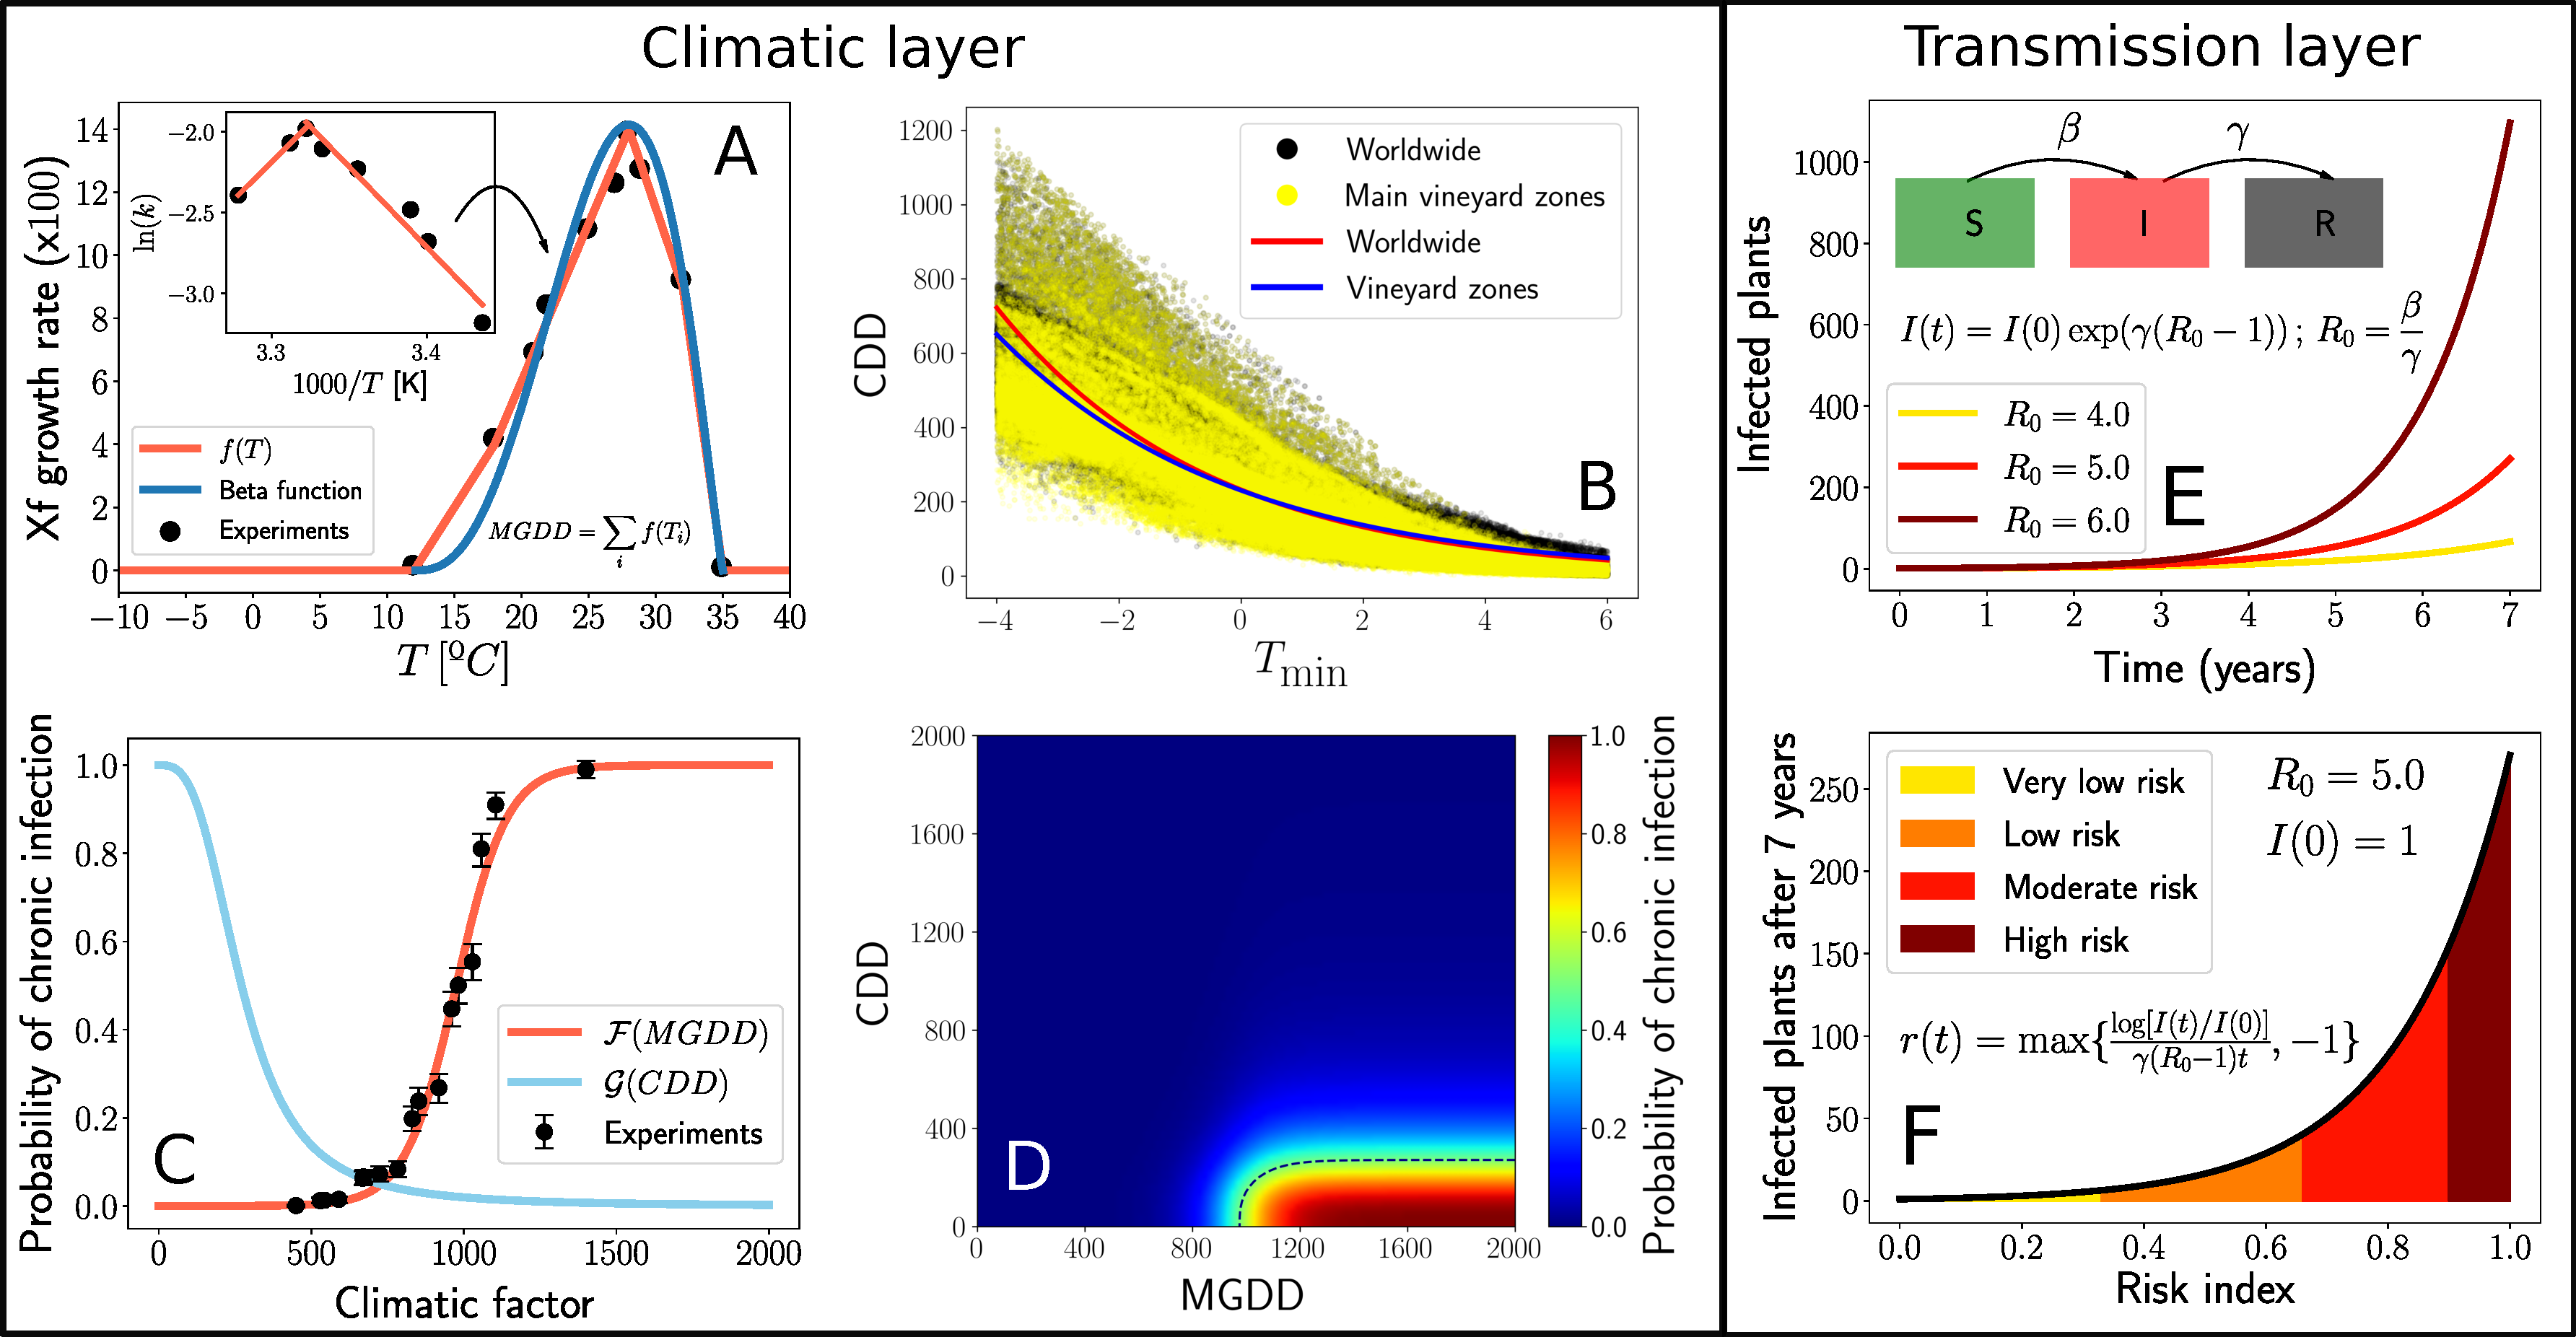
\includegraphics[width=\textwidth]{Figures/Model_h.pdf}
    \caption{\textbf{Climatic and transmission layers composing the
            epidemiological model}. (\textbf{A}) $MGDD$ profile fitted to the
        \textit{in
            vitro } data of Xf growth rate in Feil \& Purcell 2001
        \cite{Feil2001}. The
        original Arrhenius plot in Kelvin degrees (inset) was converted to
        Celsius, as
        explained in Online Supplementary Information, to obtain the main plot.
        (\textbf{B})
        Correlation between CDD and the average $T_{\textrm{min}}$ of the
        coldest month
        between 1981 and 2019. Plotted black dots (worldwide) and yellow dots
        (main
        wine-producing zones) depict climatic data from 6,487,200 cells at
        $\SI{0.1}{\degree} \cross \SI{0.1}{\degree}$ resolution, spread
        globally and
        retrieved from ERA5-Land dataset. The red solid line depicts the fitted
        exponential function for worldwide data and the blue solid line for
        main
        vineyard zones. (\textbf{C}) Nonlinear relationship between MGDD (red
        line) and
        CDD (blue line) and the likelihood of developing chronic infections.
        Black dots
        depict the cumulative proportion of grapevine plants in the population
        of $36$
        inoculated varieties showing five or more symptomatic leaves at each of
        the 15
        $MGDD$ levels (see Online Supplementary Information). Vertical bars are
        the
        95\% CI.
        (\textbf{D}) Combined ranges of $MGDD$ and $CDD$ on the likelihood of
        developing chronic infection. (\textbf{E}) Transmission layer in the
        dynamic
        equation (1) of the SIR compartmental model. (\textbf{F}) Relationship
        between
        the exponential growth of the number of infected plants with the risk
        index and
        their ranks.}
    \label{fig1}
\end{figure*}

\subsection{Thermal requirements to develop PD.}
We examined the response
of a wide spectrum of European grapevine varieties to Xf$_{\textrm{PD}}$
infection in three independent experiments conducted in 2018, 2019, and 2020.
Overall, 86.1\% ($n$ = 764) of 886 inoculated plants, comprising 36 varieties
and 57 unique scion/rootstock combinations, developed PD symptoms 16 weeks
after inoculation. European \textit{V. vinifera} varieties exhibited
significant differences in their susceptibility to Xf$_{\textrm{PD}}$
(Online Supplementary Information). All varieties, however, showed PD symptoms
to some
extent,
confirming previous field observations of general susceptibility to
Xf$_{\textrm{PD}}$ \cite{Hopkins2002, Moralejo2019, Purcell2013}.  We also
found significant differences in virulence ($\chi^2=68.73$, $\textrm{df}=1$,
$P=2.2 \cross 10^{-16}$) between two Xf$_{\textrm{PD}}$ strains isolated from
grapevines in Majorca across grapevine varieties (\cref{figS1}). Full details
on the results of the inoculation tests are available in Methods and
Supplementary
Information.

Growing degree days (GDD) have traditionally been used to describe and predict
phenological events of plants and insect pests, but rarely in plant diseases
\cite{McMaster1997}. We took advantage of data collated in the inoculation
trials together with temperature to relate symptom development to the
accumulated heat units at weeks eight, 10, 12, 14 and 16 after inoculation
(Supplementary Data 1).  Rather than counting GDDs linearly above a threshold
temperature, we consider Xf's specific growth rate \textit{in vitro} within its
cardinal temperatures. The empirical growth rates come from the seminal work by
Feil \& Purcell \cite{Feil2001} shown in the inset of \cref{fig1}A. This
Arrhenius plot is transformed, as explained in Online Supplementary
Information, to obtain a
linear approximation in a limited range of temperatures as shown in the main
plot of \cref{fig1}A. Inspired by the fit in Fig. 3 of \cite{Feil2001}, we
approximate the growth rates by a piece-wise function $f(T )$ (see Methods
below) formed by four segments. This Modified Growing Degree Day (MGDD) profile
\label{eq:MGDD_def} enables to measure the thermal integral from hourly average
temperatures, improving the prediction scale of the biological process
\cite{butikofer2020problem}. MGDD also provides an excellent metric to link
Xf$_{\textrm{PD}}$ growth in culture with PD development as, once the pathogen
is injected into the healthy vine, symptoms progression mainly depends upon the
bacterial load (i.e., multiplication) and the movement through the xylem vessel
network, which are fundamentally temperature-dependent processes
\cite{fry1990multiplication,Feil2001}. Moreover, MGDD can be mathematically
related to the exponential or logistic growth of the pathogen within the plant
(Online Supplementary Information).

Interannual infection survival in grapevines plays a relevant role when
modelling PD epidemiology. In our model, we assumed a threshold of five or more
symptomatic leaves for these chronic infections based on the relationship
between the timing and severity of the infection during the growing season and
the likelihood of winter recovery  \cite{Feil2001, Feil2003, Lieth2011}. This
five-leaf cut-off was grounded on: (i) the bimodal distribution in the
frequency of the number of symptomatic leaves among the population of
inoculated grapevines (\cref{figS1}), whereby vines that generally show less
than five symptomatic leaves at 12 weeks after inoculation remain so in the
following weeks, while those that pass that threshold continue to produce
symptomatic leaves, and (ii) the observed correlation between the acropetal and
basipetal movement of Xf along the cane (\cref{figS1}). The likelihood of
developing chronic infections as a function of accumulated MGDD among the
population of grapevine varieties was modelled using survival analysis with
data fitted to a logistic distribution $\mathcal{F}(MGDD)$. A minimum window of
$MGDD=528$ was needed to develop chronic infections (var. Tempranillo), about
975 for a median estimate, while a cumulative $MGDD>1159$ indicate over 90\%
probability within a growing season (red curve in \cref{fig1}C and Methods).

Next, we intended to model the probability of disease recovery by exposure to
cold temperatures. Previous works had specifically modelled cold curing on
Pinot Noir and Cabernet Sauvignon varieties in California as the effect of
temperature and duration \cite{Lieth2011} by assuming a progressive elimination
of the bacterial load with cold temperatures \cite{Feil2003}. In the absence of
appropriate empirical data to formulate a general average pattern of winter
curing among grapevine varieties, we combined the approach of Lieth et al.
\cite{Lieth2011} and the empirical observations of Purcell on the distribution
of PD in the US related to the average minimum temperature of the coldest
month, $T_{min}$, isolines \cite{Anas2008}. To consider
the accumulation of cold units in an analogy of the MGDD, we searched for a
general correlation between $T_{min}$ and the cold degree days (CDDs) with base
temperature = $6$ \textdegree C (see Methods). We found an exponential
relation, $CDD \sim 230\exp(-0.26\cdot T_{\textrm{min}})$, where specifically,
$CDD\gtrsim306$ correspond to $T_{\textrm{min}}<\SI{-1.1}{\degree C}$
\cref{fig1}B. To transform this exponential relationship to a probabilistic
function analogous to $\mathcal{F}(MGDD)$, hereafter denoted
$\mathcal{G}(CDD)$, ranging between 0 and 1, we considered the sigmoidal family
of functions $\displaystyle f(x)=\frac{A}{B+x^C}$ with $A=9\cdot 10^6$, $B=A$
and $C=3$ (\cref{fig1}C), fulfilling the limit $\mathcal{G}(CDD=0)=1$, i.e. no
winter curing when no cold accumulated, and a conservative 75\% of the infected
plants recovered at $T_{\textrm{min}}=\SI{-1.1}{\degree C}$ instead of 100\% to
reflect uncertainties on the effect of winter curing.

\subsection{MGDD/CDD distribution maps.}
MGDD were used to compute annual
risk maps of developing PD during summer for the period 1981-2019 (see
Methods). The resulting averaged map identifies all known areas with a
recent
history of severe PD in the US corresponding to $\mathcal{F}(MGDD) > 90\%$
(i.e., high-risk), such as the Gulf Coast states (Texas, Alabama,
Mississippi,
Louisiana, Florida), Georgia and Southern California sites (e.g., Temecula
Valley) (\cref{fig2}\textit{A}), while captures areas with a steep
gradation of
disease endemicity in the north coast of California ($\mathcal{F}(MGDD >
    50\%$). Overall, more than $95\%$ of confirmed PD sites ($n = 155$) in
    the
    US (Supplementary Data 2) fall in grid cells with $\mathcal{F}(MGDD) >
50 \%$.

    The average MGDD-projected map for Europe during 1981-2019 spots a high
    risk
    for the coast, islands and major river valleys of the Mediterranean Basin,
    southern Spain, the Atlantic coast from Gibraltar to Oporto, and
    continental
    areas of central and southeast Europe (\cref{fig2}B). Of these, however,
    only
    some Mediterranean islands, such as Cyprus and Crete, show
$\mathcal{F}(MGDD) >
99\%$ comparable to areas with high disease incidence in the Gulf Coast states
    of the US and California. Almost all the Atlantic coast from Oporto
    (Portugal)
    to Denmark are below suitable $MGDD$, with an important exception in the
    Garonne river basin in France (Bordeaux Area) with low to moderate $MGDD$
    (\cref{fig2}B).

    \cref{fig2}A shows how the area with high-risk MGDD values extends further
    north of the current known PD distribution in the southeastern US,
    suggesting
    that winter temperatures limit the expansion of PD northwards
    \cite{Hopkins2002}. A comparison between MGDD and CDD maps (\cref{fig2}A
    vs.
    \cref{fig2}C, \cref{fig2}E) further supports the idea that winter curing is
    restricting PD northward migration from the southeastern US. However,
    consistent with growing concern among Midwest states winegrowers on PD
    northward migration led by climate change \cite{Galvez2010}, we found a
    mean
    increase of $0.12 \%$ y$^{-1}$ in the areal extent with $CDD < 306$ ($\sim
T_{\textrm{min}} < -1.1$ \textdegree C) since 1981, comprising land areas
    between $103^o$W and $70^o$W of the US (\cref{fig:sup_CDD_evol}). Such an
    upward trend corresponds to $\SI{5090}{km^2}$ y$^{-1}$ in the potential
    northward expansion of PD due to climate change and an accumulation of
$\sim\SI{193420}{km^2}$ of new areas at risk since 1981.

    High-CDD values would also be expected to restrict the potential PD
    colonisation in continental Europe (\cref{fig2}D). Unlike North America,
    the
    East-West distribution of major European mountain ranges together with the
    warming effect of the Gulf Stream decreases the likelihood of cold winter
    spells reaching the western Mediterranean coast. $\mathcal{G}(CDD)$ between
    100\% and 95\% (i.e., recovery probability $<5\%$ -- low winter curing) are
    mostly prevalent below $40^o$N latitude in the southwest Iberian Peninsula
    and
    Mediterranean islands and coastlands ($<\SI{50}{km}$ away). Above $40^o$N
    latitudes, $CDD < 100$ are encountered mainly in the Atlantic coast and
    Mediterranean coast and islands (\cref{fig2}D). In contrast, central and
    southeast Europe show high CDD values likely preventing Xf$_{\textrm{PD}}$
    winter survival on infected grapevines.

    In \cref{fig2}E-F, we show the average climatic suitability for PD
    establishment only from the mechanistic relation between Xf$_{\textrm{PD}}$
    and
    temperature. Although all areas with current Xf$_{\textrm{PD}}$-related
    outbreaks are identified, risk predictions based only on the combination of
    MGDD and CDD could lead to overestimations, as this approach overlooks
    disease
    transmission dynamics and climate interannual variability.

    \begin{figure}[H]
        \centering
        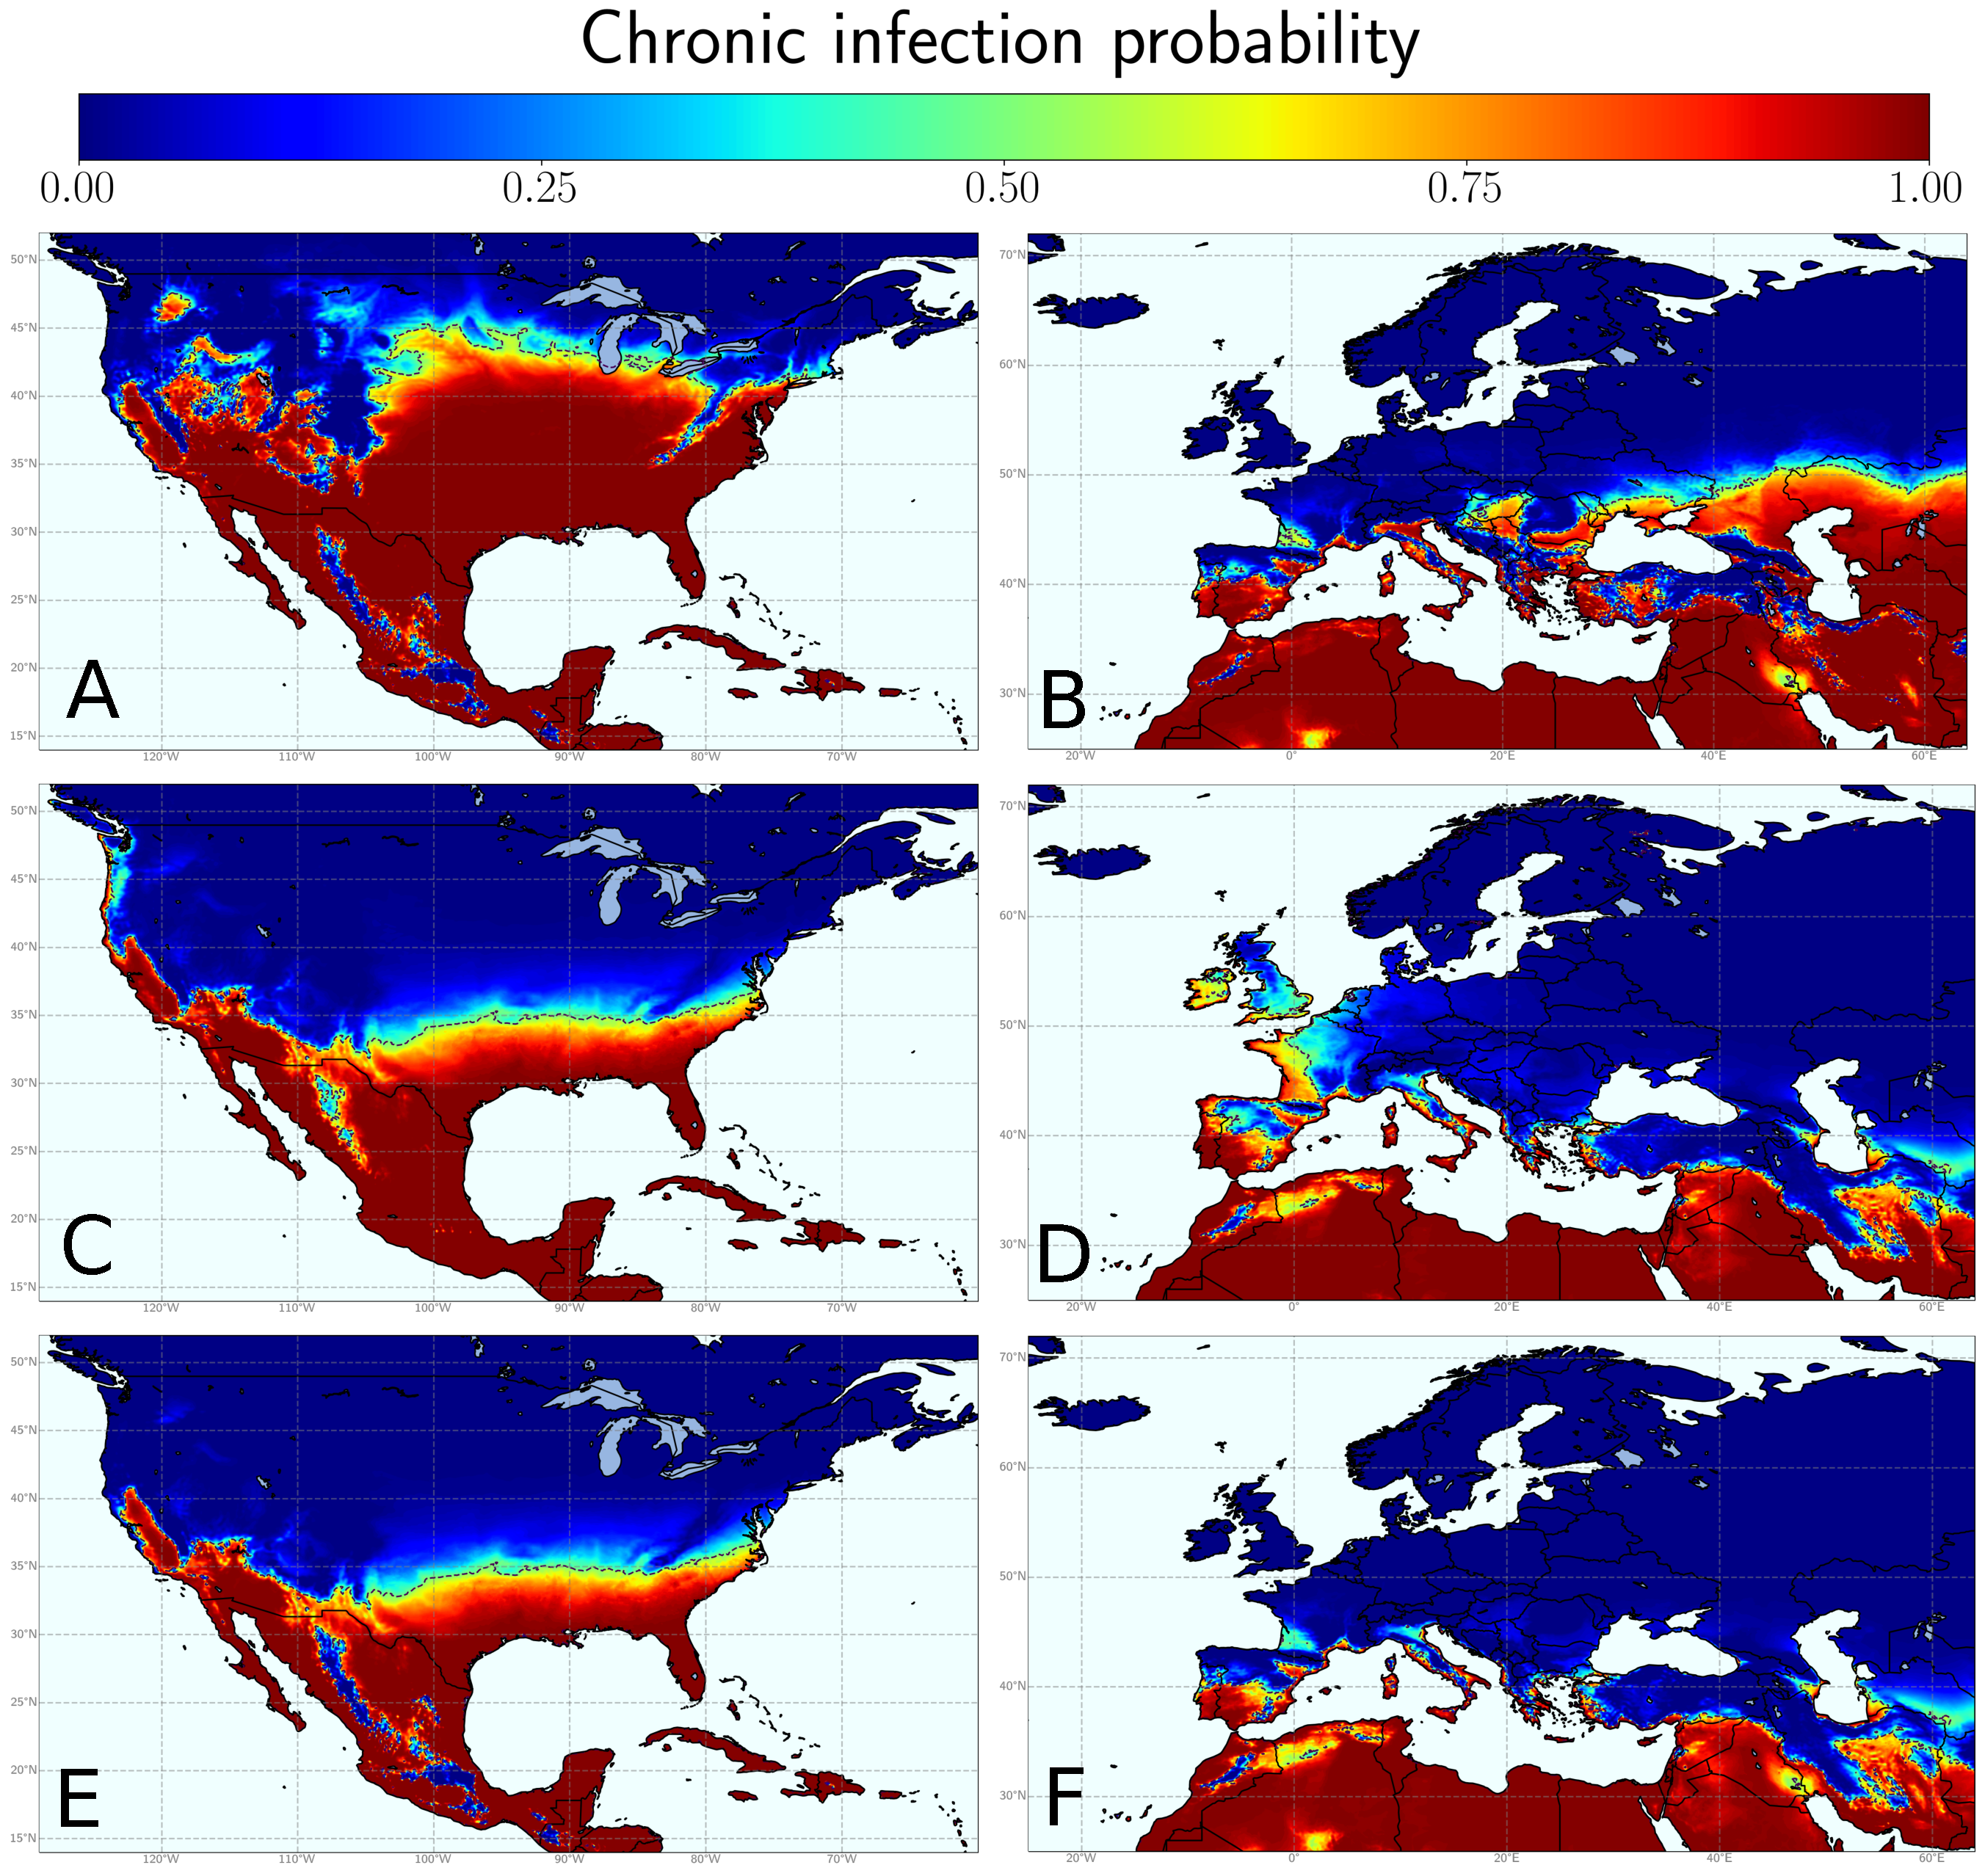
\includegraphics[width=0.85\textwidth]{Figures/Fig1_new.pdf}
        \caption{\textbf{Average thermal-dependent maps for Pierce's disease
                (PD)
                development and recovery in North America and Europe.} PD
            development during
            the growing season based on average $\mathcal{F}(MGDD)$ estimations
            between
            1981 and 2019 in North America (\textbf{A}) and Europe (\textbf{B})
            derived
            from the results of the inoculation experiments on 36 grapevine
            varieties.
            Large differences in the areal extension with favourable MGDDs can
            be observed
            between the US and Europe. The winter curing effect is reflected in
            the
            distribution of the average $\mathcal{G}(CDD)$ for the 1981-2019
            period in the
            United States (\textbf{C}) and Europe (\textbf{D}). A snapshot of
            the
            temperature-driven probability of chronic infection averaged for
            the 1981-2019
            period is obtained from the joint effect of MGDD and CDD in North
            America
            (\textbf{E}) and Europe (\textbf{F}). Warmer colours indicate more
            favourable
            conditions for chronic PD and the dashed line highlights the
            threshold of
            chronic infection probability being $0.5$.}
        \label{fig2}
    \end{figure}

    \begin{figure*}[t!]
        \centering
        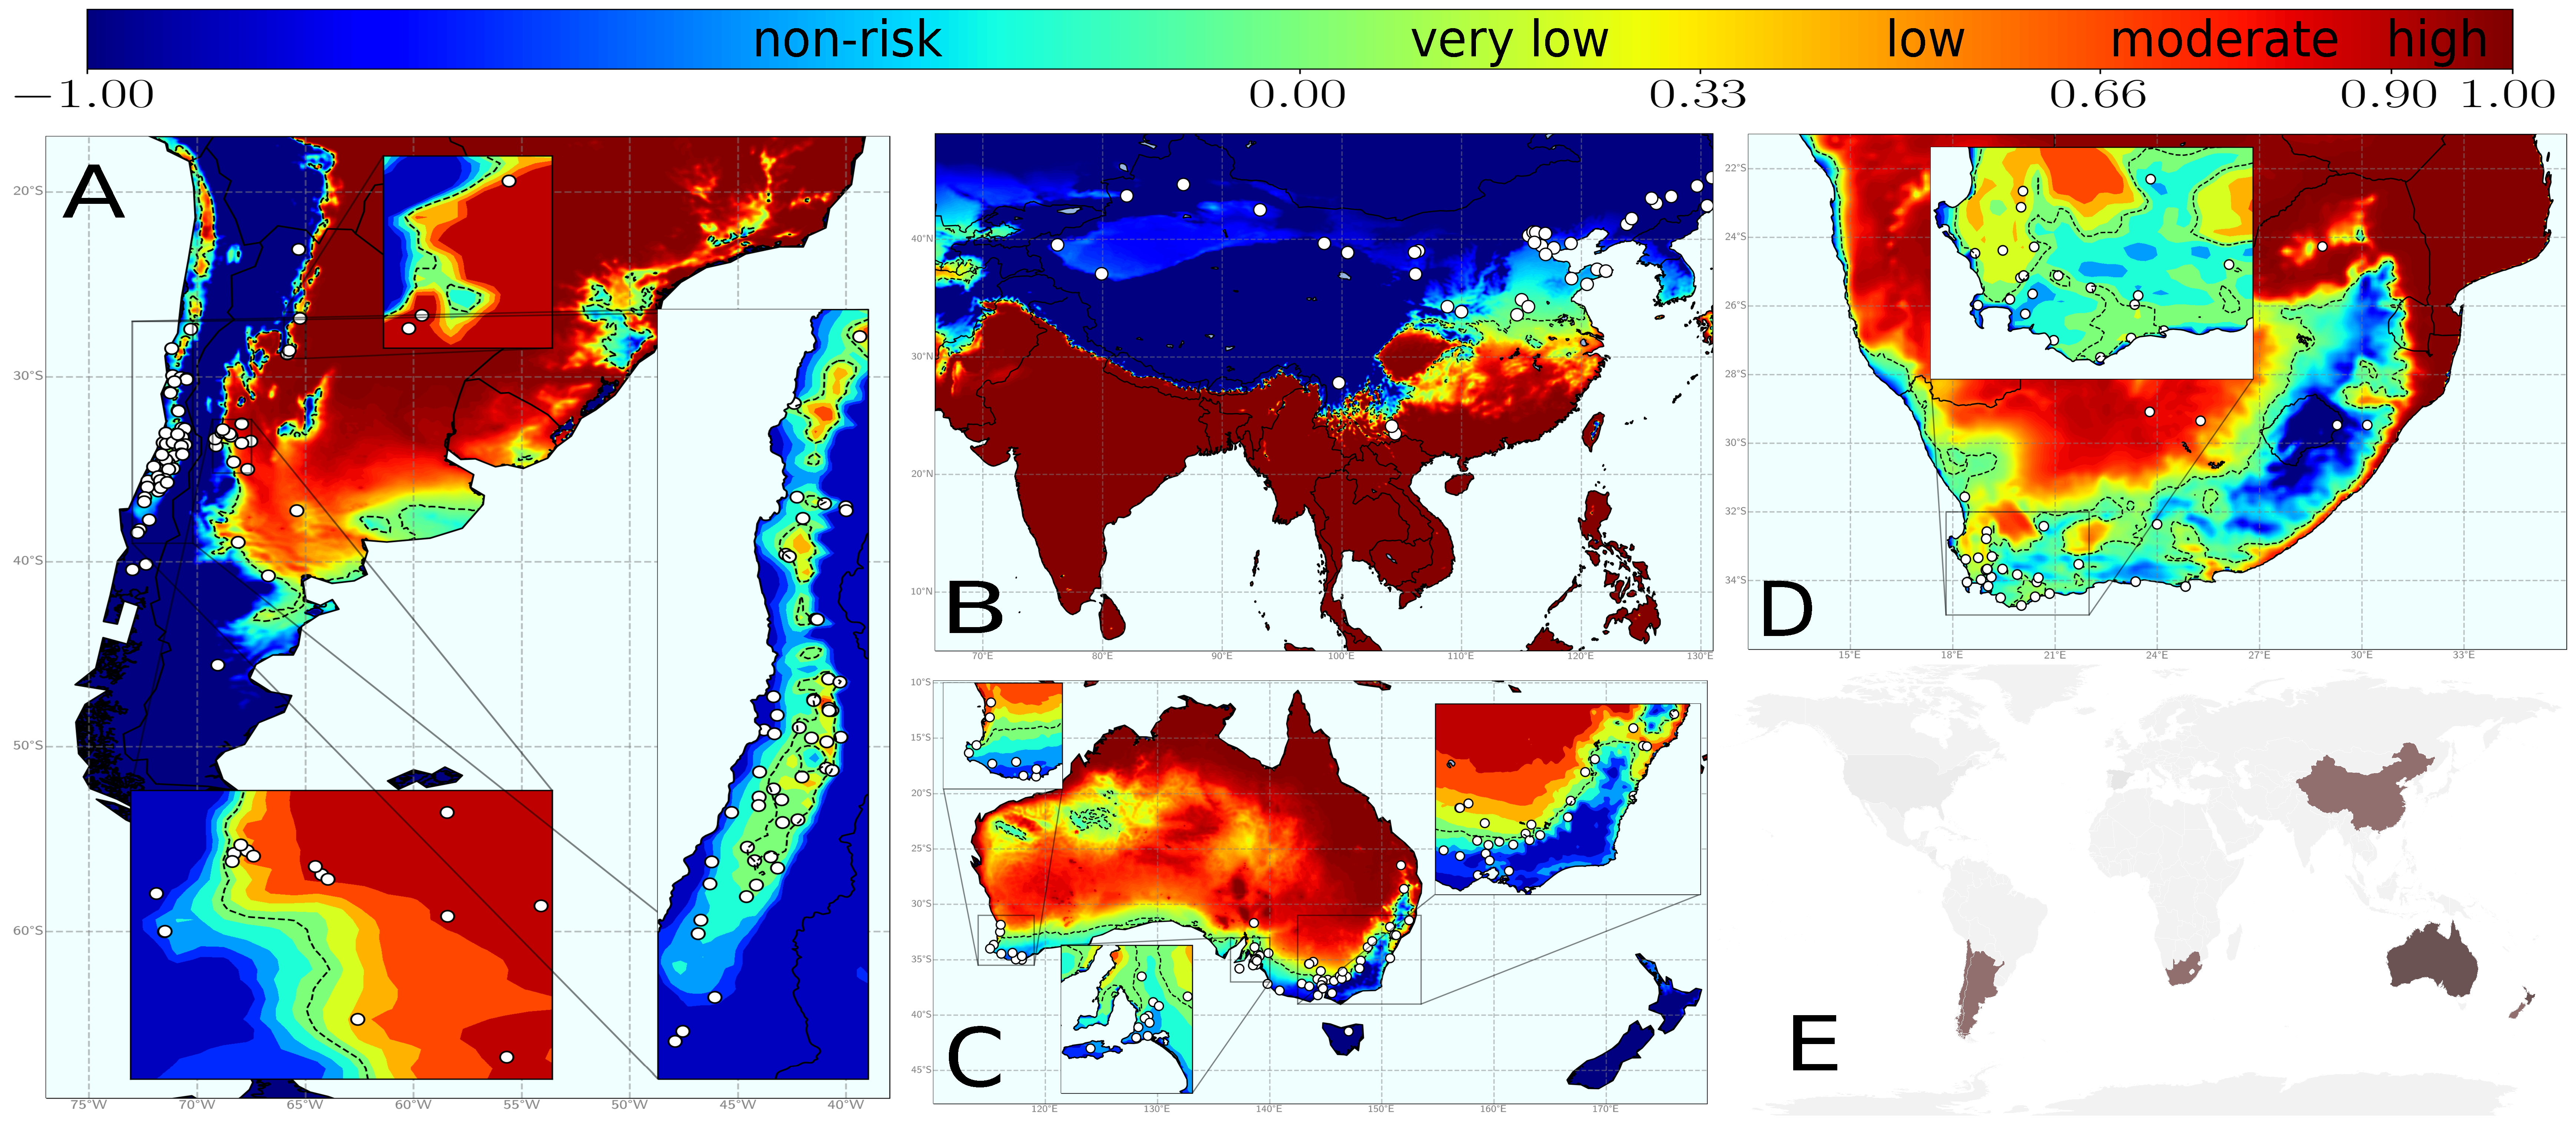
\includegraphics[width=1\textwidth]{Figures/Fig_global_risk_R0_5.pdf}
        \caption{\textbf{Climate-driven risk maps for PD establishment in main
                viticulture regions worldwide under a baseline $R_0 = 5$
                scenario.} White dots
            indicate the main vineyard areas in the wine-growing regions of
            China and the
            Southern Hemisphere. (\textbf{A}) Chile and Argentina; (\textbf{B})
            Asia with
            special attention to China; (\textbf{C}) Australia and New Zealand
            (wine areas
            are not marked as the whole country is without risk); and
            (\textbf{D}) South
            Africa. (\textbf{E}) Global distribution of main wine-producing
            areas analysed.
            The risk index $r_j(t)$, express the relative exponential growth
            rate of the
            disease incidence, and was scaled from 0.1 to 1 and ranked as very
            low
            (0.10-0.33), low (0.33-0.66), moderate (0.66-0.90) and high ($>
                0.90$).}
        \label{fig3}
    \end{figure*}

    \subsection{PD global risk.}
    We ran several simulations of the model \cref{eq:evolution_eq} with $R_0$
    values between 1 and 14 to validate PD spatiotemporal distribution in the
    US.
    We found $R_0=8$ as the optimal parameter for maximising the area under a
    ROC
    curve (\cref{fig:sup_ROC}), returning an accuracy of more than $80 \%$,
    except
    for 2006, due to data obtained from an area at the transient-risk zone
    (\cref{fig:sup_validation} and \cref{tab:validation}). For Europe and the
    rest
    of the world, we derived a $R_0=5$, as a maximal baseline estimate for
    modelling PD transmission (see Methods and Online Supplementary
    Information). These
$R_0$
    values should be taken as operating estimates for the model.  From the
    model
    simulations \cref{eq:evolution_eq}, we obtained a risk index $r$ that
    measures
    the relative exponential growth rate in the population of infected plants
    at
    the epidemic onset with respect to the maximum growth, $r=1$. This index
    served
    to rank the epidemic-risk zones in high ($> 0.9$), moderate ($0.66-0.9$),
    low
    ($0.33-0.66$) and very low ($\sim 0.075-0.33$) risks (see \cref{fig1}F,
    Methods, and Online Supplementary Information).

    \begin{table}[H]
        \begin{center}
            \caption{\textbf{Validation of model predictions.} The items are
                locations
                where PD was present or absent. TP corresponds to true
                positives and TN to true
                negatives according to our model with $R_0=8$. }
            \label{tab:validation}
            \resizebox{0.8\textwidth}{!}{%
                \begin{tabular}{llllll}
                    \hline
                    Year  & Presence & Absence & TP & TN & Accuracy \\
                    \hline
                    2001  & 16       & 5       & 15 & 3  & 86\%     \\
                    2002  & 12       & 2       & 11 & 1  & 86\%     \\
                    2005  & 4        & 2       & 4  & 1  & 83\%     \\
                    2006  & 8        & 0       & 4  & 0  & 50\%     \\
                    2015  & 53       & 0       & 51 & 0  & 96\%     \\
                    \hdashline
                    TOTAL & 93       & 9       & 85 & 5  & 88\%     \\
                    \hline
                \end{tabular}
            }
        \end{center}
    \end{table}

    To date, PD is mainly restricted to the American continent with some
    unrelated
    introductions of Xf$_{\textrm{PD}}$ to Taiwan and Majorca (Spain) from the
    United States \cite{Moralejo2019,Su2013}. To assess the risk of PD
    establishment elsewhere, we projected our epidemiological model into the
    main
    winegrowing regions of the Northern Hemisphere (US, Europe and China) and
    Southern Hemisphere (Chile, Argentina, South Africa, Australia and New
    Zealand)(\cref{fig3}A-E). We found that emerging wine-producing areas in
    China
    are predominantly located in non-risk zones, whereas only some vineyards in
    the
    Henan and Yunnan provinces fall in transition and moderate-high risk zones
    (\cref{fig3}B and Supplementary Data 3). In Europe, 92.1\% of the territory
    is
    in non-risk zones and 6.1\% is included in the epidemic-risk zone, with
    only
    1.9\% showing a high-risk index and 1.5\% a moderate risk
    (Online Supplementary Information).
    The model also reveals a progressive transition from areas without risk
    ($r(t)
< 0$) before 1990 to epidemic-risk zones with low-risk indexes by 2019
    (\cite{Webpage}, see Movies), mainly affecting the basins of the rivers Po
    in
    Italy, Garonne and Rhone in France and Douro/Duero in Portugal and Spain.
    This
    represents a mean increase of $0.21\%$ y$^{-1}$ in the epidemic-risk zone,
    a
    rate $3.5$-times greater than that of the eastern US, which could increase
    the
    likelihood of PD establishment in Europe in the coming decades. In the US,
    most
    states around the Gulf Coast show high-risk indexes, whereas, around 37.5\%
    of
    California's surface is suitable for epidemics with high growth rate
    incidence
    (Online Supplementary Information).

    In the Southern Hemisphere, vineyards at non-risk or transient
    epidemic-risk
    zones predominate -- e.g., non-risk in New Zealand and Tasmania
    (\cref{fig3}C).
    Risk indexes in areas where PD can become established ($r(t) > 0$) range
    from
    very low to low for most coastal vineyards in Australia (west, south and
    east)
    with somehow more suitable conditions in the interior of New South Wales,
    Greater Perth and Queensland (\cref{fig3}C); a general very-low or low-risk
    indexes are predicted in the Western Cape in South Africa (\cref{fig3}D);
    overall very-low but localised low to moderate risk indexes in some areas
    in
    Chile; and low to moderate growth of the number of infected vines in most
    of
    Argentina, being this the wine-growing country with the highest risk
    (\cref{fig3}A). Detailed information on areas with non-risk, transient risk
    and
    risk indexes (i.e., disease-incidence growth rates) in areas with the
    potential
    risk of establishment by country and regions is provided in Supplementary
    Information.

    \begin{figure}[H]
        \centering
        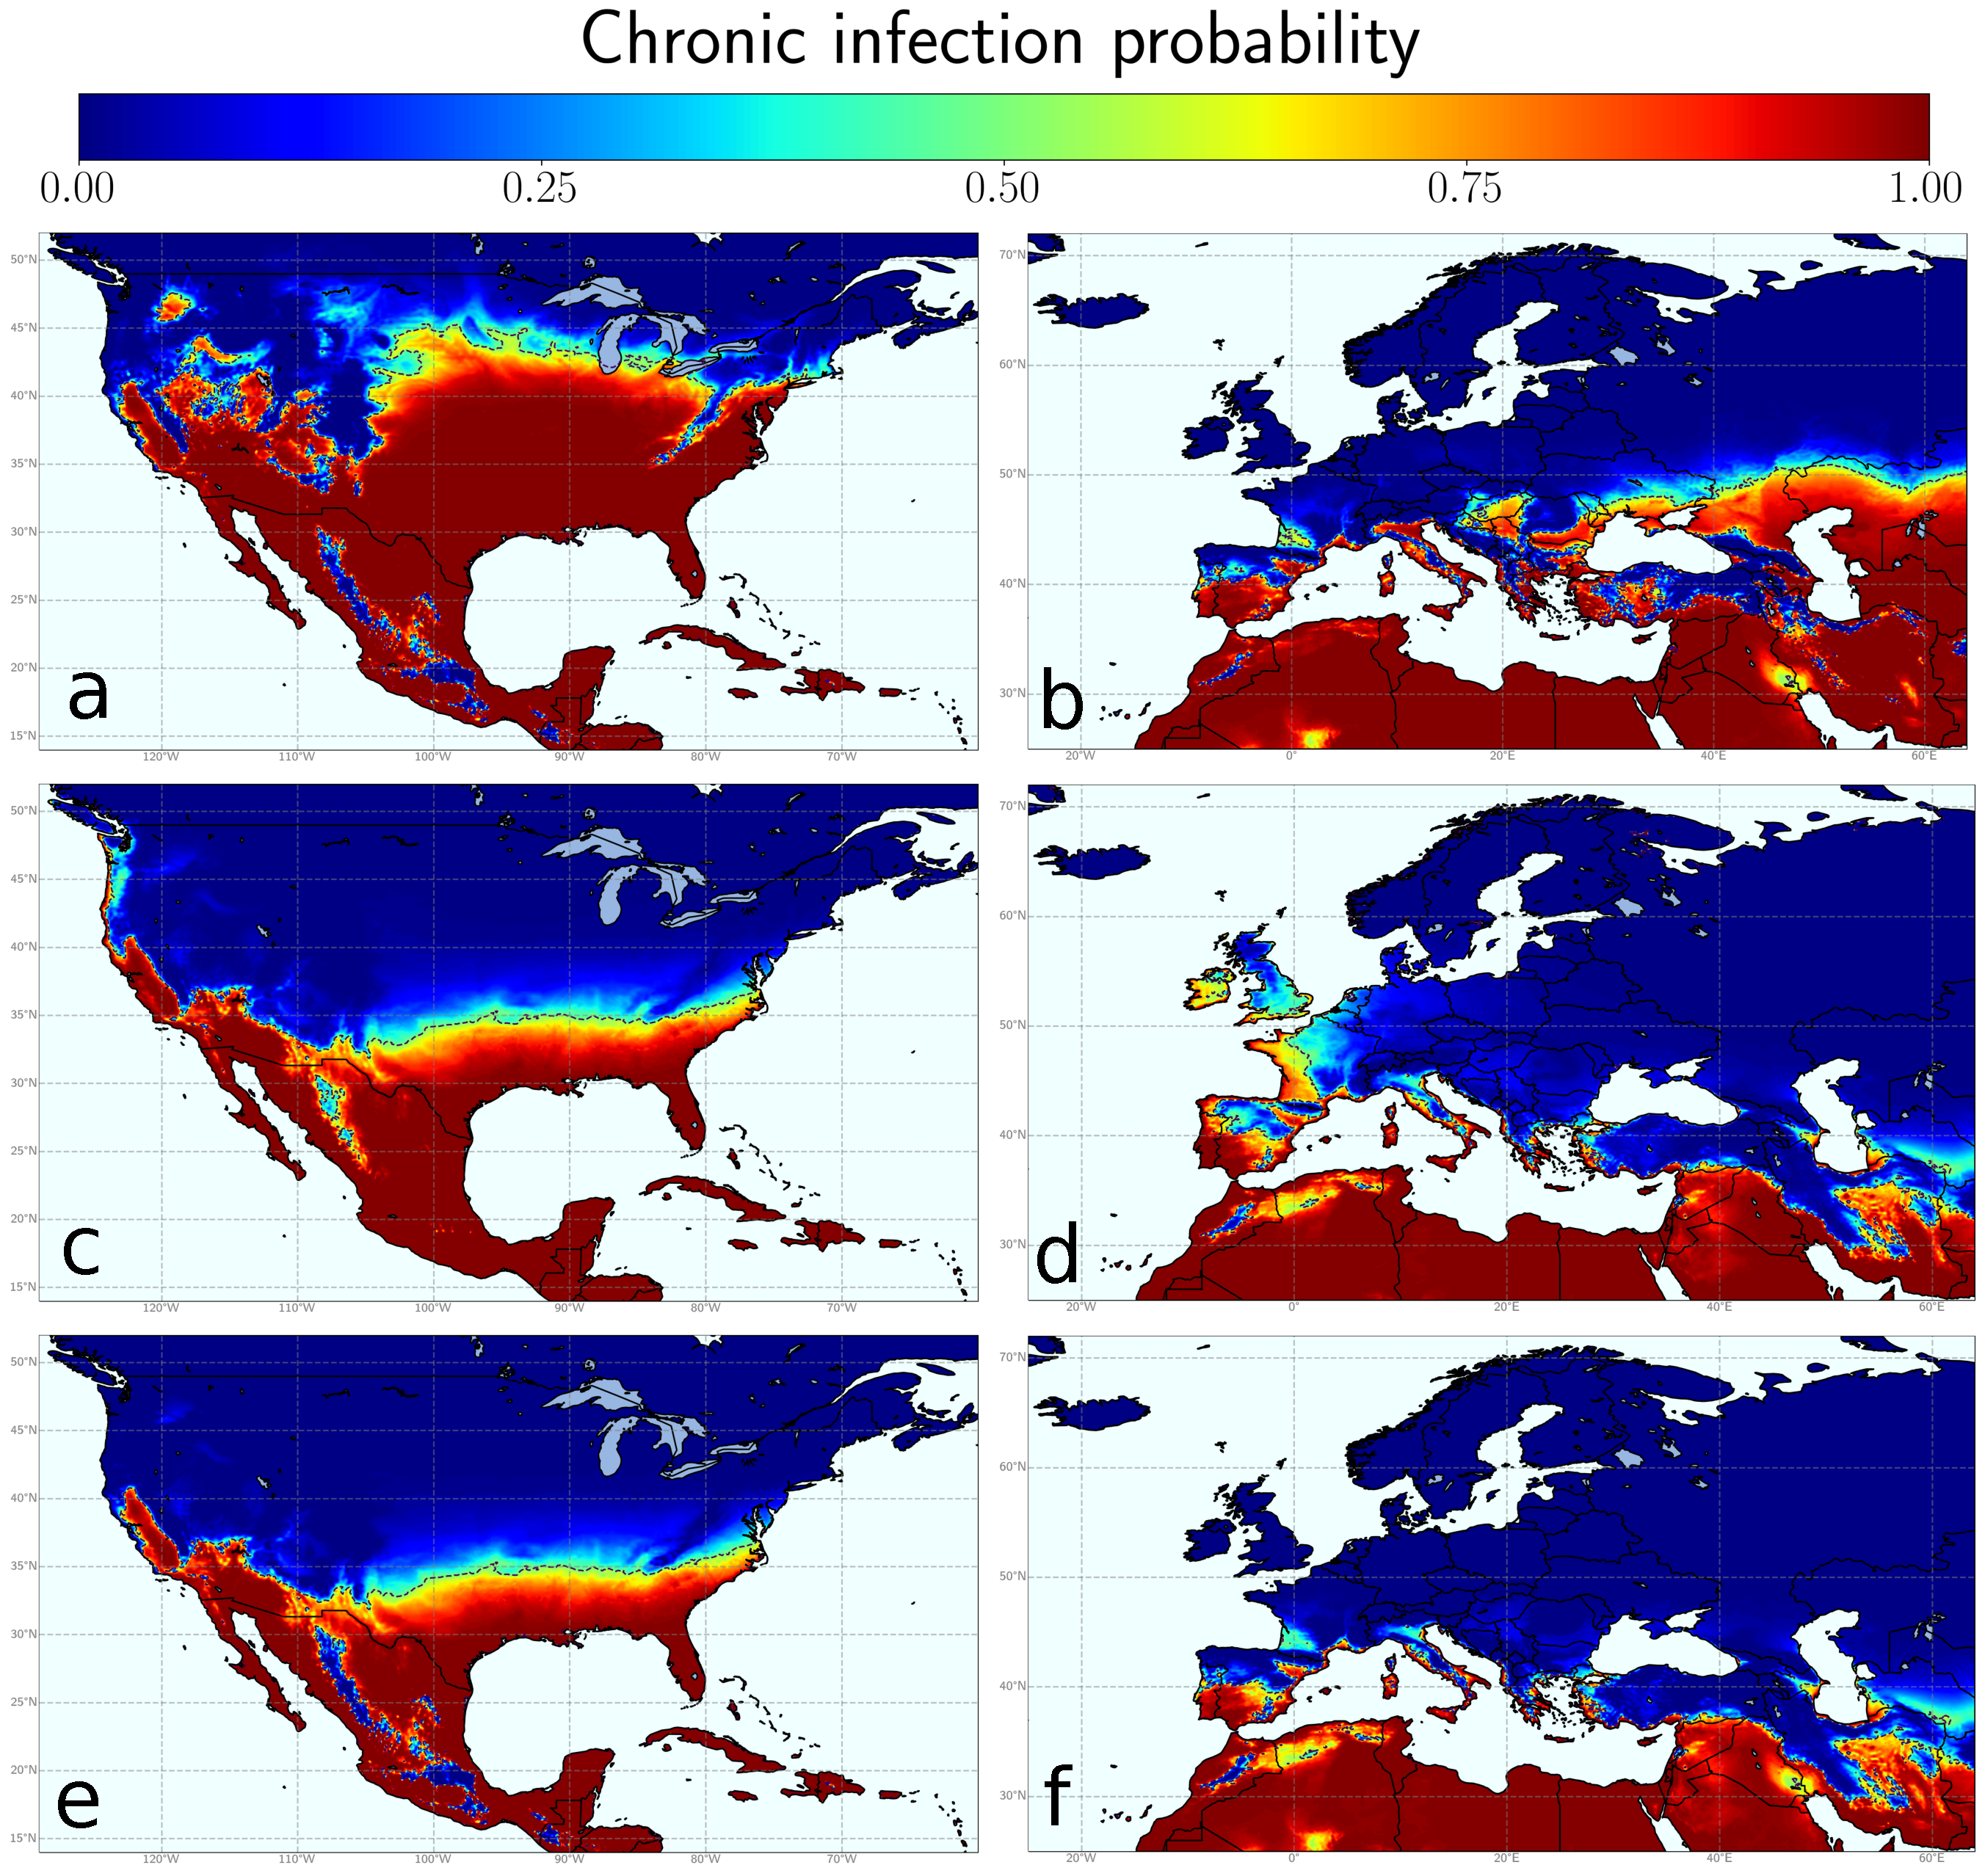
\includegraphics[width=0.9\textwidth]{Figures/Fig2.pdf}
        \caption{\textbf{Temperature-driven dynamic-model simulations  for PD
                establishment from 1981 to 2019 under different $R_0$ scenarios
                with a
                spatially homogeneous vector distribution.} For comparison, the
            baseline
            scenario with a $R_0=5$ for Europe is projected to North America
            (\textbf{A})
            capturing to some extent the distribution and severity of PD in
            that continent.
            In Europe (\textbf{B}) high-risk areas (i.e., $r_j(t) > 0.90$) are
            restricted
            to coastal Mediterranean and the south of the Iberian Peninsula;
            black dash
            line separate areas with $r(t)>0$ where theoretically PD can
            thrive. Under
            higher $R_0$ scenarios, $R_0=8$ for North America (\textbf{C}) and
            Europe
            (\textbf{D}), the dash lines tend to separate from isoline
            $T_{\textrm{min}} =
                -1.1$\textdegree C (white line); and even more in extreme
            transmission pressure
            $R_0=16$ for North America (\textbf{E}) and Europe (\textbf{F}). }
        \label{fig4}
    \end{figure}

    Risk indexes may vary within epidemic-risk zones if any of the
    epidemiological
    parameters governing transmission change. As expected, $I(t) < I(0)$
    boundaries
    increasingly displace to northern latitudes in the US and Europe under
    higher
    transmission scenarios, increasing the risk-epidemic zones significantly
    (\cref{fig4}A-F). The line representing the outbreak extinction i.e., the
    non-risk zone $r(t)<-0.09$, in the validated $R_0=8$ scenario for the US,
    falls
    at some distance above the isoline $T_{\textrm{min}} = -1.1^o$C in
    comparison
    to the $R_0=5$ scenario (\cref{fig4}, \cite{Webpage}). This distribution
    pattern holds and moves slightly northward over
    time
    in parallel to global warming, although the trend of PD latitudinal change
    is
    moderated by high-CDD values (i.e. cold accumulation). In addition, the
    disease
    extension also declines due to CDD interannual fluctuations in the
    simulations.
    Cold waves periodically occur that reach latitudes close to the Gulf, such
    as
    those that occurred in 1983, 1993, 1995, 2000, 2009 and 2013 (Movies at
    \cite{Webpage}), thus preventing PD expansion northward. The magnitude of
    this
    decrease is revealed after comparing the average annual increase of the
    areas
    between $r(t) > 0$ and $CDD < 306$ lines. From 1981 to 2019, the area with
    risk
$r(t) > 0$ increased at a rate of $0.05\%$ y$^{-1}$, while that of $CDD < 306$
    by $0.12\%$ y$^{-1}$, an important difference not explained alone by CDDs
    without considering climate fluctuations (\cref{fig:sup_CDD_evol}).

    \subsection{PD risk projections for 2050}. Global shifts in the risk
    index
$r_j(t)$ between 2019 and those projected for 2050 were calculated under the
    same baseline scenario (\cref{fig5}A-F, Methods). Our simulation shows a
    generalised increasing trend mainly due to shifts from transition zones to
    epidemic-risk zones with very low or low-risk indexes in the main
    wine-growing
    regions, except for the US. Here the epidemic-risk zone would increase by
$12.8\%$ with the greater increments in the high-risk index category ($22.7\%$)
    and a decrease in the transition zones (Online Supplementary Information).
    Much
    less surface
    would be included in the epidemic-risk zone in Europe ($8.6\%$) compared to
    the
    US ($36.5\%$). However, the epidemic-risk zone would expand by $40.0\%$
    with
    respect to 2020, a rate more than three times higher than that of the US
    (Online Supplementary Information). Such increases are due to the emergence
    of
    previously
    unaffected areas in 2020 evolving into epidemic-risk zones by 2050, and
    epidemic growth-rate increases in already epidemic-risk zones in 12 of 42
    countries (Online Supplementary Information). Among these 12 countries,
    however,
    there is
    substantial variation in the risk index increments within epidemic-risk
    zones
    with respect to 2019 (Online Supplementary Information). While non-risk
    zones
    still cover
$87.6\%$ of Europe's land area, epidemic-risk zones with high-risk indexes are
    expected to be almost two-fold higher than that of 2019, comprising $3.2\%$
    of
    Europe (\cref{table2}). \\

    \begin{figure*}[b!]
        \centering

        \includegraphics[width=\textwidth]{Figures/Fig_global_risk_change_R0_5.pdf}
        \caption{\textbf{Global shifts in PD risk index ($r_j(t)$) from 2020 to
                2050.} To build the maps, we have assumed a spatial homogeneous
            vector
            distribution and a $R_0=5$ scenario, except for the US where a
            $R_0=8$ has been
            used in the model simulations.\textbf{(A)} North
            America;\textbf{(B)}
            Europe;\textbf{(C)} Asia; \textbf{(D)} South America; \textbf{(E)}
            Australia
            and New Zealand; and \textbf{(F)} South Africa. Risk-index
            increases are in red
            and decreases in blue. The dashed line represents the spatial
            threshold where
            $r_j(t)$ difference changes from negative to positive.}
        \label{fig5}
    \end{figure*}

    \begin{table*}[t!]
        \centering
        \caption{\textbf{Shifts in risk areas for Pierce's disease in Europe
                projected
                for 2050 under a $R_0$ = 5 scenario.} The model was run
            assuming the same
            homogeneous spatial distribution of the vector for the whole
            period.}
        \begin{tabular*}{\hsize}{@{\extracolsep{\fill}}lllllll}
            \hline
            Risk & 2050 & 2020 & Difference & Difference & 2050 & 2020 \\
            & km$^2$ & km$^2$ & km$^2$ & (\%) & (\%) area & (\%) area \\
            \hline
            No risk & $8885300.5$ & $9334178.7
            $ & $-448878.2
            $ & $-4.8
            $ & $87.6
            $ & $92.1
            $ \\
            Transition & $381081.3$
            & $182872.6$ & $198208.7$ & $108.3$ & $3.8$ & $1.8$ \\
            Very low & $189025.3$ & $179225.7
            $ & $9799.6$ & $5.5$ & $1.9$ & $1.8$ \\
            Low & $207599.4$ & $104143.1$ & $103456.3$ & $99.3$ & $2.1$ & $1.0$
            \\
            Moderate & $154780.5$ & $148621.4$ & $6159.0$ & $4.1$ & $1.5$ &
            $1.5$ \\
            High & $322225.9$ & $190971.4$ & $131254.5$ & $68.7$ & $3.2$ & $1.9
            $ \\
            \hline
        \end{tabular*}
        \label{table2}
    \end{table*}

    \subsection{Risk based on vector information}. So far, we have ignored
    the
    distribution of known and potential vector species due to their large
    number in
    the Americas and the limited quantitative information generally available.
    In
    the case of Europe, given \textit{P. spumarius} prevalence as a potential
    vector and its wide distribution, we added	a vector layer in a spatially
    dependent $R_0(j) = R_0^{\textrm{max}}\, v(j)$, where $v(j)$ is the
    climatic
    suitability for the vector (Methods), $v=1$ implies optimal climatic
    conditions
    with no constraints for the vector population size, while $v=0$ implies
    unsuitable climatic conditions and its absence (\cref{fig:sup_vector}).
    According to the model, no European zone shows a high-risk index and barely
$0.34\%$ of the territory falls in areas with potential moderate exponential
    growth rates in disease incidence (Online Supplementary Information).
    Irrespective
    of
    vineyard
    distribution, we estimated that PD could potentially become established
    (i.e.,
$r(t) > 0$) at a maximum of $3.1\%$ of the territory, while the area at
    moderate-risk index would be $5$-times lesser than the model without the
    vector's climate suitability layer, this latter more in consonance with
    other
    proposed risk maps \cite{Godefroid2019,Bragard2019}. Such differences in
    the
    projected risks are mainly concentrated in the warmest and driest
    Mediterranean
    regions and are due to uncertainties concerning temperature-humidity
    interactions in the ecology of the vector \cite{Godefroid2021}.

    \begin{figure*}[H]
        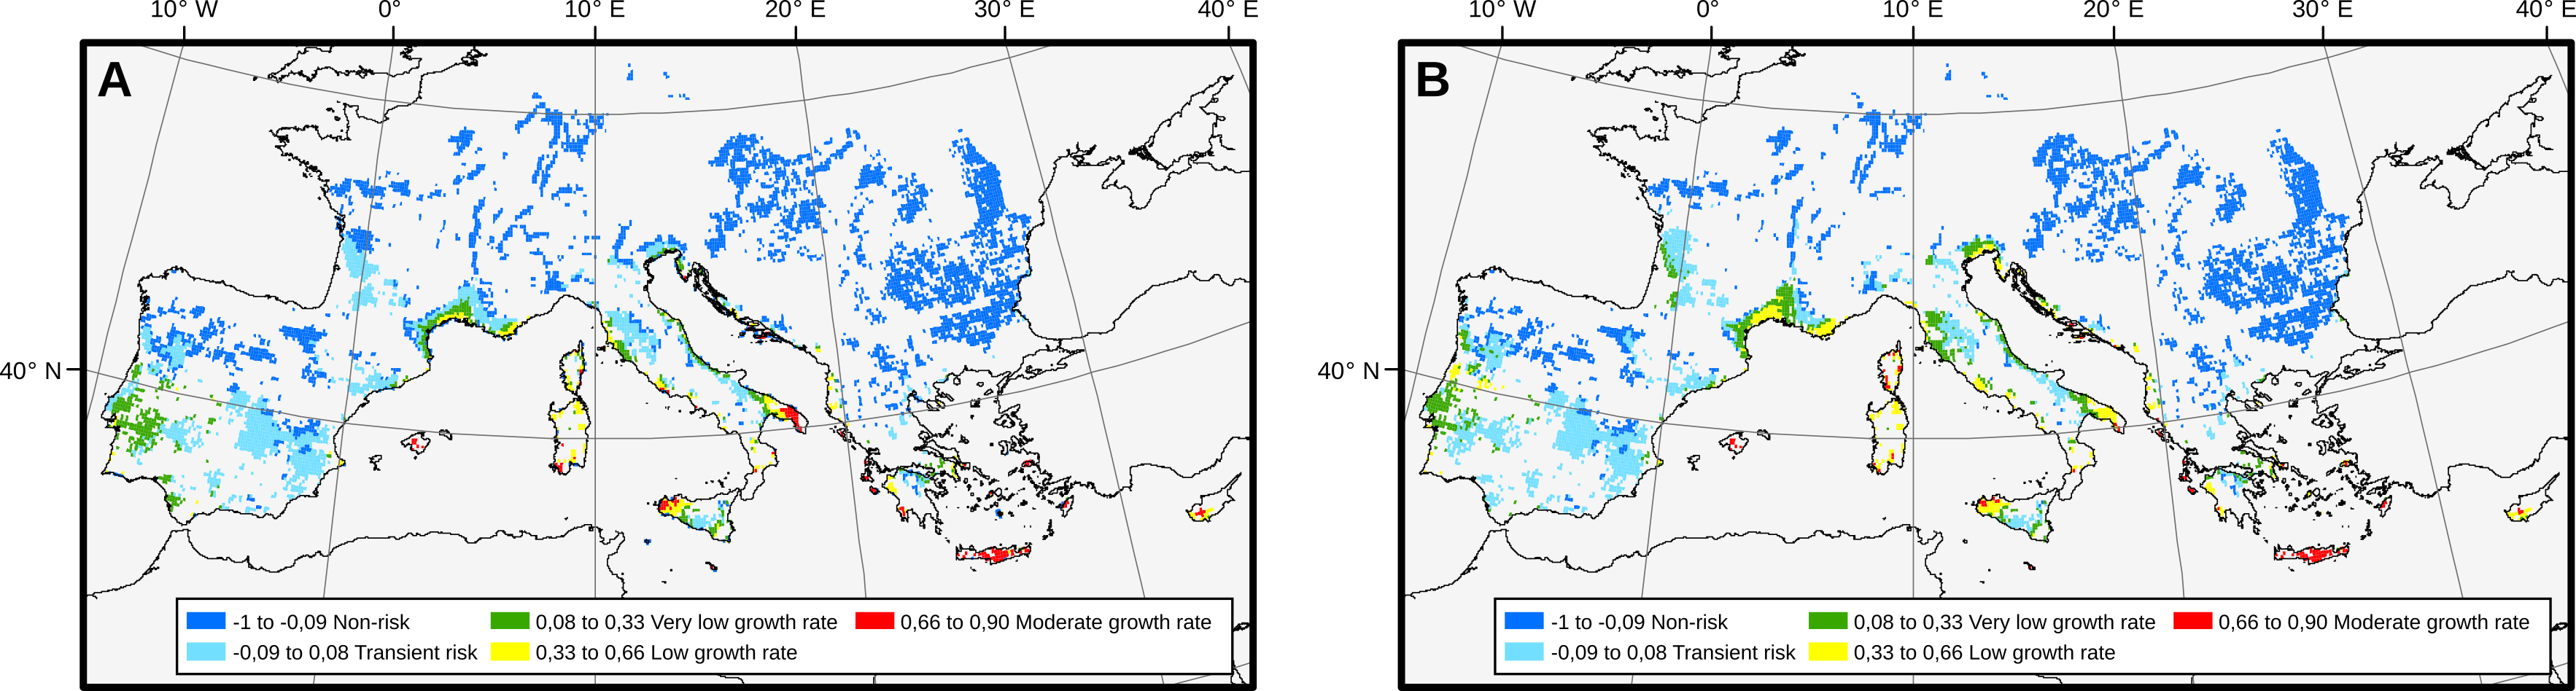
\includegraphics[width=1\textwidth]{Figures/vineyards.png}
        \caption{\textbf{Intersection between Corine-land-cover vineyard
                distribution map and PD-risk maps for 2020 and 2050.}  Data
            were obtained from
            Corine-land-cover (2018) and the layer of climatic suitability
            for\textit{P.
                spumarius} in Europe from \cite{Godefroid2021}. The surface of
            the vineyard
            contour has been enlarged to improve the visualisation of the risk
            zones and
            disease-incidence growth-rate ranks. \textbf{(A)} PD risk map for
            2019 and its
            projection for 2050 \textbf{(B)}. Blue colours represent non-risk
            zones and
            transient risk zones for chronic PD ($R_0 < 1$). The 2050 map shows
            some
            contraction of epidemic-risk zones with moderate risk indexes in
            Mediterranean
            islands and Apulia (Italy) as the climate becomes hotter and
            dryer.}
        \label{fig6}
    \end{figure*}

    \subsection{Combining vineyard land cover across Europe with the model
        output.}
    When we integrate into the model a layer of vineyard surface from
    Corine-Land-Cover, we find that PD could potentially become established
    (i.e.,
$r(t)>0.075$) in $22.3\%$ of the vineyards in Europe. However, no vineyard is
    in epidemic-risk zones with a high-risk index and only $2.9\%$ of the
    vineyard
    surface is at moderate risk (Online Supplementary Information). The areas
    with the
    highest
    risk
    index ($r(t)$ between $0.70$ and $0.88$) are mainly located in the
    Mediterranean islands of Crete, Cyprus and the Balearic Islands or at
    pronounced peninsulas like Apulia (Italy) and Peloponnese (Greece) in the
    continent (\cref{fig6}A and Online Supplementary Information).  Most
    vineyards are
    in
    non-risk
    zones ($42.1\%$), whereas $35.6\%$ are located in transition zones with
    presently non-risk but where Xf$_{\textrm{PD}}$ could become established in
    the
    next decades causing some sporadic outbreaks. In Online Supplementary
    Information,
    we provide full details of the total vineyard areas
    currently
    at risk for each country and region.

    Our model with climate and vector distribution projections for 2050
    indicates a
$ 55.8 \% $ increase in the epidemic-risk zone in Europe (\cref{fig6}B). This
    increment would be mainly due to the extension of epidemic-risk zones with
    very
    low and low-risk indexes. However, within the epidemic-risk zones, areas
    with
    moderate risk indexes would decrease from $\SI{114925}{ha}$ in 2020 to
$\SI{43114}{ha}$ in 2050, and no vineyards would be at high risk (\cref{fig6}B;
    see Online Supplementary Information). Counterintuitively, our
    model
    indicates a substantial increase in the area where PD could establish and
    become endemic for 2050, but a moderate decline in those areas where crop
    damage could be expected to be significant (e.g., Balearic Islands, Crete,
    Cyprus, Apulia).

    \section{Discussion}

    We introduce an epidemiological approach to assess the risk of PD
    establishment
    and epidemics in vineyards worldwide. The model includes the dynamics of
    the
    infected-host population, which enables estimating the initial exponential
    growth/decrease rate of the disease incidence. Unlike SDM correlative
    studies,
    Bayesian or, in general, machine learning black-box approaches, our model
    goes
    beyond by providing a mechanistic framework and thus explanatory power. In
    addition, it is flexible enough to simulate different climate and
    transmission
    scenarios, allowing, for instance, the incorporation of information on the
    spatial distribution of the vector. Comprehensive global PD risk maps
    result
    from the model simulations with historical climatic data. A web page is
    included, showing simulations with different parameters to estimate the
    risk of
    PD anywhere \cite{Webpage}.

    Temperature regulates key physiological processes of the ectothermic
    organisms
    involved in PD and thus limits the thermal range in which they can thrive
    \cite{Coakley1999}. Xf$_{\textrm{PD}}$ multiplication and survival within
    vine
    xylem vessels not only characterise PD, but also determine the bacterial
    population dynamics \cite{fry1990multiplication,Feil2001}. PD symptom
    development can be therefore characterised as a thermal-dependent
    continuous
    process within the range of  Xf$_{\textrm{PD}}$'s cardinal temperatures
    \cite{Scherm1994}. The combination of MGDD metrics with robust experimental
    data provides a reliable predictor of climatic suitability and the
    probability
    of developing PD during the summer, whereas CDD accounts for the effect of
    cold-temperature exposure on infected-plant recovery. This opposite
    contribution of MGDD and CDD in the demography of infected plants shapes
    the
    impact of climate variability on the epidemic dynamics in the early stages
    of
    the invasion (\cref{fig1}D). Given that the physiological basis of the
    plant-Xf
    interaction leading to symptoms development is poorly understood, we
    caution
    that other environmental factors, such as drought, nutrient status or crop
    management may modulate symptom expression and hence add an error in the
    MGDD
    parameter not measured in this work. Also, another limitation is that the
    relation between MGDD and Xf$_{\textrm{PD}}$ growth rates come from in
    vitro
    experiments and we assume that it is valid in planta as well. Nonetheless,
    we
    deem the error range would be smaller than the differences in the
    accumulated
$MGDD$s needed to reach the same disease level among varieties (i.e., regional
    differences) and smaller than the interannual $MGDD$ oscillations found in
    most
    locations.

    Knowledge of insect distribution is crucial for predicting epidemic
    outbreaks
    of endemic diseases, as well as the risk of invasion by emerging
    vector-borne
    pathogens (\cite {Caminade2017,Jeger2019}, (cf. \cite{Schneider2020})).
    Given
    the great diversity of known and potential vectors that can transmit PD
    \cite{Redak2004}, it has not been possible to include each region's
    particular
    vectors in the model. Therefore, when evaluating the risk of PD on a global
    scale, we have considered a homogeneous spatial distribution of the vector
    (fixed $ R_0 $), except in Europe where there is information on the main
    vector
    (\cref{fig:sup_vector}). As expected, the European case shows how models
    that
    assume a homogeneous spatial distribution of the vector generally produce
    epidemic risk zones with higher risk indexes than models that include a
    heterogeneous spatial distribution.
    This
    lack of information about vectors is one of the main reasons why the risk
    of
    vector-borne plant diseases is often overestimated.

    Risk overestimations may involuntarily stem from other additional sources
    too.
    Using mean data as inputs in epidemiological models can lead to biased
    results
    when response functions are nonlinear and climate variability is not
    accounted
    for \cite{Scherm1994}. This study presents experimental evidence of a
    non-linear relationship between MGDDs and PD chronic infections and
    indirect
    empirical evidence of a non-linear relationship between CDDs and PD
    recovery
    (\cref{fig:sup_climatic_oscilations}). Such a non-linear response
    consequently
    greatly impacts reducing the risk of PD establishment and steeping the
    spatial
    gradients in risk maps (\cref{fig4,fig6}). Moreover, MGDDs and CDDs might
    help
    to explain why disease pressure is much higher in the southeastern US than
    in
    California and Europe (\cref{fig2,fig4}) or, for example, earlier reports
    of PD
    outbreaks in Kosovo  \cite{Berisha1998}. Cooler summer nights in California
    and
    a shorter growing season compared to those found in the Gulf states in the
    southeastern US explain the difference in the accumulated $MGDD$ for both
    areas. In the case of Kosovo, $CDD$ values above certain thresholds could
    have
    led to the extinction of incipient outbreaks driven by several years with
$MGDD$ in the conducive range of PD (\cref{fig2}).

    Our PD risk map for Europe confirms previous predictions for the subsp.
    \textit{fastidiosa} from SDMs \cite{Bragard2019}. Both approaches make
    congruent predictions on PD potential distribution, providing convergent
    lines
    of independent evidence of climate suitability. However, our risk maps go
    further by incorporating in the epidemic-risk zones information on the
    relative
    exponential growth rates in the potential disease incidence. In general
    terms,
    the epidemic-risk map including vector information indicates low risk for
    chronic PD. Only $\sim 0.34\%$ of European vineyard surface, mainly located
    in
    Cyprus, Crete, Sardinia, part of Sicily and the Balearic Islands, meet
    climatic
    conditions for PD to become endemic and cause significant damage
    (Online Supplementary Information). Other regions such as Bordeaux,
    Portugal, Rh\^one Valley, and the Veneto region, would be included in
    epidemic-risk zones but with very low to low exponential growth rates in
    disease incidence. By contrast, notorious wine-growing regions in Spain
    (e.g.,
    Rioja, Ribera del Duero), France (e.g., Burgundy) and Italy (e.g.,
    Piedmont)
    currently fall within areas considered as non-risk zones,
    transient-epidemic
    zones or epidemic-risk zones with very-low risk indexes (\cref{fig6}).

    The dynamic nature of the simulation outputs already points to a
    progressive
    global increase in the areal extension of PD epidemic-risk zones ($r(t)>0$)
    in
    the last decade, irrespective of vineyard distribution (see movies on
    \cite{Webpage}). This is even more accentuated in the model projections for
    2050, which point out a global expansion of PD epidemic-risk zones at
    different
    velocities among continents due to climate change (\cref{fig5}). For
    example,
    many important viticulture areas in western Europe included in non-risk or
    transition zones before 1990 are progressively shifting to hotter summers
    and
    milder winters and hence would be increasingly suitable for the disease
    within
    the extrapolated current scenario. This is further illustrated by a $40\%$
    increase of the potential epidemic-risk zone by 2050 concerning 2020 for
    Europe
    and more moderate increases in the United States and the Southern
    Hemisphere
    (\cref{fig5}). Nonetheless, our model projection for 2050 that includes
    spatial
    heterogeneity in the vector distribution, as in Europe, would indicate
    lower
    transmissibility because global change is predicted to have negative
    effects on
    \textit{P. spumarius} abundance in Europe \cite{Godefroid2021,Karban2018}.
    At
    the global scale, there is certainly scientific consensus that climate
    change
    will follow a general pattern summarised in the paradigm "dry gets drier,
    wet
    gets wetter" \cite{Feng2015}. In agreement, our model projection for PD on
    vineyards of Majorca (Spain) suggests shifts to slightly less favourable
    conditions for Xf$_{\textrm{PD}}$ transmission and an expected progressive
    decrease in the impact of the disease by 2050. This example and others in
    Mediterranean islands (see Supplementary Data 4) advocate for certain
    caution
    when interpreting climate change projections, especially in other
    Mediterranean
    climates of the world, where the complex interactions between humidity and
    temperature can limit the presence and abundance of vectors
    (\cref{fig:sup_vector}).

    The scope of our study excludes location-specific complexities surrounding
    PD
    ecology due to scale limitations. The spatial distribution of the vector is
    considered only for the \textit{V. vinifera}-Xf$_{\textrm{PD}}$-{\textit{P.
        spumarius}} pathosystem in Europe, so $R_0$ estimations could locally
    differ in
    other wine-producing regions elsewhere (\cref{fig3}). Disease incidence
    thus
    could locally vary where the climate is conducive to PD. Such variation is
    because transmission rates tend to increase exponentially rather than
    linearly
    under environmental conditions favouring vector abundance
    \cite{Gruber2012}, as
    has been observed at a local scale on vineyards of Majorca
    \cite{Moralejo2019}.
    Our study also does not contemplate likely changes within the PD
    pathosystem.
    To date, PD is caused by Xf$_{\textrm{PD}}$ (i.e., ST1/ST2), but other
    genotypes of the subsp. \textit{fastidiosa} or other subspecies and their
    recombinations could arise in the future with different ecological and
    virulence traits \cite{Vanhove2019}. On the other hand, new vector species
    could be accidentally brought in \cite{Redak2004}, as exemplified with the
    introduction of the glassy-winged sharpshooter (\textit{Homalodisca
        vitripennis}) in California, modifying transmission rates and disease
    incidence
    in new areas \cite{Daugherty2019}. To capture these uncertainties in
    relation
    to the vector, we have performed simulations with $R_0 = 8$ and $R_0 = 16$
    (\cref{fig4}). Remarkably, a comparison of PD risk maps for Europe with
    different $R_0$ suggests for non-Mediterranean areas the need to stress
    more
    surveillance on the introduction of alien vectors rather than in the
    pathogen
    itself. This is because, under the current scenario ($R_0$ = 5) with
    \textit{P.
        spumarius} as the main vector, most of the non-Mediterranean vineyards
    would
    not support the establishment of PD, but the introduction of new insect
    vectors
    with greater transmission efficiency ($R_0=8$) could compensate the
    climatic
    layer and increase the risk index above 0. In addition, differences in
    grapevine varietal response alongside virulence variation among Xf strains
    may
    slightly modify PD thermal tolerance limits and therefore locally modulate
    epidemic intensity (see details in Online Supplementary Information). Such
    effect
    could be seen with cv. Tempranillo, a widely planted variety in northern
    Spain
    (Online Supplementary Information); the rate of symptom progress and
    systemic movement is
    higher
    than the average varietal response to Xf$_{\textrm{PD}}$ (i.e., lower
$MGDD$),
    which in addition might imply higher survival rates. This point calls for
    further testing in the field.

    Our model partially explains why PD has not become established in
    continental
    Europe and other main wine-growing regions worldwide during the last 150
    years,
    in contrast to other exotic diseases and pests brought in with native vines
    from the US \cite{Borkarbook, Brewer2010, Rouxel2014, Tello2019}. We
    suggest
    that the underlying causes of this low-invasiveness risk in Europe are
    fundamentally two: (i) low climatic suitability for chronic PD and (ii) a
    climatic mismatch between environment conditions suitable for both the
    vector
    and the pathogen and their interplay in disease dynamics, similar to the
    situation recently described for the \textit{V.
        vinifera}-Xf$_{\textrm{PD}}$-{\textit{P. spumarius}} pathosystem in
    northern
    California \cite{Beal2021}. Currently, suitable conditions for the
    pathogen's
    invasion mostly concur in Mediterranean islands and coastlands
    (Supplementary
    Data 4). Likewise, similar results would be expected in other Mediterranean
    climates of main winegrowing regions of the Southern Hemisphere if a vector
    spatial distribution layer is incorporated in the model simulations (see
    \cite{Webpage}). Finally, although increasing global warming will extent
    epidemic-risk zones in all continents, some caution is recommended to not
    incur
    risk overestimation, as we show in the PD risk projections for 2050 in
    Europe
    when taking into account the vector spatial distribution; complex
    interactions
    between temperature and humidity in the ecology of the vectors may have a
    great
    effect in their distribution, abundance and thus transmission capacity
    \cite{Godefroid2021}. There is an urgent need to fill the knowledge gap on
    the
    ecophysiology for each potential vector to downscale PD model predictions
    to
    local and regional situations.

    \section{Methods}

    \subsection{Inoculation tests.} Xf$_{\textrm{PD}}$-inoculation tests
    were
    conducted in 2018, 2019 and 2020. A sample of 36 local, regional and
    international wine-grape varieties was selected, which included nine of the
    10
    most cultivated wine-grape varieties representing more than 80\% of the
    worldwide vineyard surface (https://www.oiv.int). Plants were randomly
    distributed in 12-plant rows along an insect-proof net tunnel and exposed
    to
    environmental temperature. In total, 57 rootstock-scion combinations were
    pin-prick mechanically inoculated \cite{Almeida2003} with two strains of
    Xf.
    subsp. \textit{fastidiosa} (ST1) isolated from grapevines in Majorca.
    Disease
    severity was rated by counting the number of symptomatic leaves eight weeks
    after inoculation in mid-May and then every two weeks until the 16th week
    \cite{Moralejo2019}. Full details on the inoculation conditions, isolates,
    disease score and statistical analysis are provided in Supplementary
    Information.

    \subsection{Modified Growing Degree Days.} We generalized McMaster \&
    Wilhelm’s \cite{McMaster1997} formulation of growing-degree days to account
    for
    the growth rate of Xf$_{\textrm{PD}}$ as a function of temperature under
    optimal culture conditions based on the well-known Arrhenius law valid in
    the
    relevant temperature range for Xf (Online Supplementary Information).
    Specific growth rate
    ($k$) values at different temperatures were extracted from the publication
    of
    Feil \& Purcell \cite{Feil2001} to build the mathematical function $f(T)$
    describing the Xf’s instantaneous growth rate dependence on temperature
    according to
    \begin{align*}
         & f(T)=\left\{\begin{array}{lll}
                           0                & \textrm{if} & T<T_{\textrm{base}}
                           \\
                           m_1\cdot T-b_1   & \textrm{if} & T_{\textrm{base}}
                           \leq T < T_1
                           \\
                           m_2\cdot T + b_2 & \textrm{if} & T_{1} \leq T <
                           T_{\textrm{opt}}
                           \\
                           m_3 + b_3        & \textrm{if} & T_{\textrm{opt}}
                           \leq T < T_2
                           \\
                           m_4 + b_4        & \textrm{if} & T_2 \leq
                           T_{\textrm{max}}
                           \\
                           0                & \textrm{if} & T\geq
                           T_{\textrm{max}}
                       \end{array}\right. \,
    \end{align*}
    where $T_{\textrm{base}}=\SI{12}{\degree C}$, $T_1=18$,
$T_{\textrm{opt}}=\SI{28}{\degree C}$,	$T_2=32$ and
$T_{\textrm{max}}=\SI{35}{\degree C}$; the slopes are $m_1= 0.66$, $m_2=1$,
$m_3=-1.25$ and $m_4=-3$ and the intercepts are $b_1=-8$, $b_2=-14$, $b_3=4$
    and $b_4=105$.

    MGDD is then defined as:
    \begin{equation}\label{eq:MGDD_def}
        MGDD(t) = \frac{1}{24}\sum_{\tau \in t} f(T(\tau)),
    \end{equation}
    where $\tau$ is expressed in hours, $t$ in years and we divide by $24$ to
    obtain $MGDD(t)$ in degree days.

    \subsection{Disease progress with temperature.} Hourly mean
    temperature
    data were recorded between April 1 and October 31 in 2018, 2019 and 2020
    with
    an automated weather station (Quimisur, IQ2000). The temperature sensor was
    at
    a two-meter height from the bare ground and around five meters from the
    entrance of the insect-proof net tunnel. To characterise the progress of PD
    symptoms, we converted into $MGDD$ units the cumulative hourly mean
    temperatures measured from the time of inoculation to the day of disease
    evaluation using \cref{eq:MGDD_def}. In total, 15 $MGDD$ levels were
    estimated corresponding to weeks 8, 10, 12, 14, and 16 after inoculation in
    the
    years 2018, 2019, and 2020, respectively. Data on the number of symptomatic
    leaves (severity) for each plant and MGDD levels were pooled in a single
    database to seek a generalized average thermal response pattern among the
    population of \textit{V. vinifera} varieties (see Supplementary Data 1). To
    model the probability of chronic infections (i.e., persistent year-to-year
    infections), we used a survival analysis, where the event of interest
    depends
    on the cumulative MGDD rather than time. First, we defined a chronic
    infection
    cut-off point to transform the number of symptomatic leaves into binary
    data.
    Previous research had evidenced that early grapevine infections, in
    addition to
    producing more extensive and severe PD symptoms, are more likely to survive
    the
    following year than late infections (\cite{Feil2001, Feil2003, Lieth2011}.
    Furthermore, susceptible cultivars generally show lower recovery
    percentages
    compared to the less susceptible ones in the field
    \cite{purcell1974spatial,purcell1981vector}. Similarly, we observed in our
    inoculation assays that the majority of infections that reach around five
    or
    more symptomatic leaves 12 weeks after inoculation continue to develop more
    symptomatic leaves the following weeks, while for plants that do not exceed
    that threshold, symptoms tend to remain stagnant. These results indicate a
    low
    probability of survival for infections showing few symptomatic leaves
    during
    the growing season and thus support our heuristic approach of assigning
    five or
    more symptomatic leaves as a threshold for chronic infection (see
    Supplementary
    Information and \cref{figS1} for assumptions of chronic infection). Using
    the
    "survival" package in R \cite{survival-package}, we analysed the cumulative
    probability of developing chronic infections as a function of $MGDD$.
$F(MGDD)$ was adjusted to the experimental data by the nonlinear least squares
    method. The 10th, 33rd, 50th, 66th, and 90th percentiles were used to scale
    the
    risk of the total $MGDD$ in the logistic function, $\mathcal{F}(MGDD)$
    (\cref
    {fig1}C).

    \subsection{Disease recovery through winter curing.}  We modelled
    winter
    curing considering the effect of temperature duration below a threshold
    temperature, where we assume that the bacterial killing process increases
    in
    efficiency with decreasing temperatures \cite{Lieth2011}. To adjust a
    probabilistic model to the accumulation of cold units, we took as reference
    the
    distribution and severity of PD in the US proposed by Purcell based on the
    isolines of the mean $T_{ min}$ of the coldest month (available in
    \cite{Anas2008}) where PD is rare ($T_{ min}$ between $-1.1$ \textdegree C
    and
$1.7$ \textdegree C), occasional ($1.7-4.5$\textdegree C) and severe ($>
4.5$\textdegree C). Noteworthy, the projection of these isolines in Europe has
    predicted with some precision the distribution of the establishment of Xf
    in
    the continent \cite{Bragard2019}. To capture the accumulation nature of the
    chilling process at different climatic zones, we determined the global
    average
    correlation between $T_{\textrm{min}}$ and the average accumulated CDD
    between
    November 1 and March 31 in the northern hemisphere and between April 1 and
    October 31 in the southern hemisphere using 6,487,200 points distributed
    throughout the planet. The $CDD$ was estimated as
    \begin{equation}
        CDD(t)= \frac{1}{24}\sum_{\tau \in t} (6-T(\tau)) \ \quad \textrm{for}
        \quad T_i\le 6\textrm{\textdegree C} ,
    \end{equation}
    where the threshold $6 \textrm{\textdegree C}$ comes from Ref.
    \cite{Lieth2011}.

    \subsection{Global climate data, MGDD/CDD computation.}
    Global mean hourly temperature data were downloaded from the ERA5-Land
    dataset
    \cite{ERA5_dataset} at $0.1^o$ spatial resolution using GRIB format. The
    annual
    average $T_{\textrm{min}}$ of the coldest month was calculated from the
    hourly
    average temperature from the ERA5-Land dataset. To calculate the annual
$MGDD$
    and $CDD$ a simple Julia \cite{julia} library was built on top of GRIB.jl
    package \cite{GRIB}. For the Northern Hemisphere, the accumulated $MGDD$s
    were
    computed from April 1 to October 31, whereas ($CDD$s) were estimated from
    November 1 to March 31, and the reverse for the Southern Hemisphere.

    \subsection{Disease Model.} We used a standard
    susceptible-infectious/infected-recovered (SIR) compartmental model to
    assess
    the risk of PD establishment and epidemics worldwide, represented by the
    following three equations in the large population limit:
    \begin{equation}
        \begin{array}{l}
            \dot{S}=-\beta \, S \, I/N ,         \\
            \dot{I}=\beta S\, I/N - \gamma\,  I, \\
            \dot{R}=\gamma \, I \ ,
        \end{array}
        \label{eq:SIRmodel}
    \end{equation}
    where $S$ is the susceptible host population, $I$ is the infected
    population, $R$ is the dead population and $S+I+R=N$ is the total number of
    vines in the population. The reduction of a vector-borne disease model to a
    SIR
    model gives rise to a linear dependence of the basic reproductive number
$R_0$
    on the vector population (see Online Supplementary Information).
    Vector-plant
    transmission
    of the pathogen is approximated with an effective plant-to-plant
    transmission
    rate $\beta$ (Online Supplementary Information), as has been done
    previously
    for
    other Xf-related diseases \cite{White2020}, and the transition from the
    infected compartment to the recovered (dead) compartment is given by the
    recovery (mortality) rate $\gamma$.  In a mean-field approximation of the
    onset
    of an outbreak, the basic reproductive number ($R_0=\beta/\gamma$) defines
    the
    exponential growth/decrease stage in the SIR model (\cref{fig1}E,
    Online Supplementary Information). Although the time from infection to vine
    death depends on
    the
    environmental conditions and the grape wine variety, we assigned a
    mortality
    rate of $\gamma$ = 0.2 y$^{-1}$  based on the estimated median survival
    time of
    infected vines in California \cite{Almeida2003}. The maximum growth rate of
    the
    epidemic, relevant for an estimation of the risk of establishment, occurs
    when
$S(t=0)\sim N$, and was approximated by the (linearized) differential equation,
    \begin{equation}
        dI/dt \approx \beta \, I-\gamma \, I = \gamma\,  I\, (\beta/\gamma -
        1)=\gamma \, I\, (R_0-1) \ ,
    \end{equation}
    where we have assumed the initial conditions:
$S(t= 0)\approx N$, $I(t = 0)= I(0) \approx0$ and $R(t = 0)=0$. This linear
    differential equation can be integrated exactly:
    \begin{equation}\label{eq: infect_proc}
        I(t)=I(0)\, \exp(\gamma\, (R_0-1)\, t) \ .
    \end{equation}

    To account for the effect of temperature in the epidemic process, we modify
    the previous expression as follows
    \begin{align}
        \label{eq: final_eq}
        I(t) & =I(0)\, \exp(\gamma\, (R_0-1)\, t)\,
        \mathcal{F}\parentesi{MGDD(t)}\,
        \mathcal{G}\parentesi{(CDD(t)} \nonumber
        \\
             & =I(0)\, \exp(\gamma(R_0-1)t)\, \Pi(t) \ ,
    \end{align}
    where $\Pi(t)=\mathcal{F}(MGDD(t))\, \mathcal{G}(CDD(t))$ is the cumulative
    probability of chronic infection dependence on temperature and $R_0$ bears
    the
    information on the vector density.

    The spatial unit of the model is given by the resolution of the ERA5-Land
    data, for which we assume uniform conditions within each of the grid cells
    (approximately $9 \times 9\,  \textrm{km}^2$) in terms of vector
    population,
    susceptible vines and parameters that define the model. Risk outcome is
    calculated for each cell of the spatial raster individually; i.e., there is
    no
    simulated spread from one cell to another. Altogether, the equation
    representing the number of individuals with chronic infections in each cell
$j$
    at time $t$ is written as
    \begin{equation}\label{eq:evolution_eq}
        I_j(t)=\underbrace{I_j(t-1) \, e^{\gamma \,
                    (R_0(j)-1)}}_\text{transmission
            layer}	  \overbrace{\Pi_j(t)}^\text{climatic layer} ,
    \end{equation}
    where $I(t-1)$ is the number of chronic infections in the previous year
    ($t-1$) and $\Pi_j(t)=\mathcal{F}(MGDD)\, \mathcal{G}(CDD)$ is the climatic
    layer that modulates the growth term and describes the cumulative
    probability
    of new infections becoming chronic in the time period between $t-1$ and
$t$.
    The model assumes a homogeneous distribution of the vector population among
    the
    grid cells (same $\beta$ and then same $R_0(j) = R_0$) except for Europe,
    where
    information on the spatial distribution of \textit{P. spumarius} is
    available
    (see Methods). In this latter case, a spatial dependent $R_0(j)$ is
    incorporated into the model by considering the product of the homogeneous
$R_0$
    and the spatially-dependent climate suitability for vectors
    (Online Supplementary Information).

    To compute the epidemic-risk maps, we carried out a simple simulation
    summarized in three steps: (i) at the initial condition for the first year
    considered, $t_0$, each grid cell is seeded with a single infected plant,
$I(t_0)=1$; (ii) the simulation runs for a year and the incidence is calculated
    following \cref{eq:evolution_eq}; (iii) we seed again the cells for which
    the
    number of infected plants has vanished. In the last seven years of the
    simulation, there is no reseeding to allow the system to relax. This
    process is
    repeated until the final year $\mathcal{T}$. Finally, the risk index
$r_j(\mathcal{T})$ is calculated from the final number of infected plants at
    grid cell $j$ as
    \begin{equation}
        r_j=\textrm{max}\left\{\frac{\log(I_j(\mathcal{T})
            /I_j(t_0))}{\gamma\,
            (R_0(j)-1)\, \mathcal{T}}, -1 \right\} \ .
        \label{eq:riskmeasure}
    \end{equation}
    In this equation, $r_j$ implicitly delimits three differential risk zones
    in the maps: 1) a non-risk zones where $r_j \le -0.09$, and the number of
    infected plant decreases exponentially; 2) a transition areas where $-0.09
< r_j \le 0.075 $, and 3) an epidemic risk-zone where $ r_j >0.075$ and PD
    can
    theoretically become established and produce an outbreak --the number of
    infected plants increases exponentially (see Online Supplementary
    Information for
    further
    details.)

    Model performance was calibrated with observed records of PD presence in
    California and the southeast of the US, where the disease is well
    established.
    PD distribution data were collected from publications from 2001 to 2020.
    Publications were filtered by selecting only records where the pathogen
    detection on symptomatic grapevines was confirmed by PCR or Elisa. The
    exact
    coordinates of the records were taken when available in the publication or
    approximated to locality or county level to build the Supplementary Data 1
    \cite{Overall2015, Vanhove2019, Lieth2011, Anas2008, Hail2009,
        Wallingford2007,
        Myers2007, Albibi1998}. For modelling purposes and to attempt a general
    rough
    estimate of the $R_0$ parameter valid for the entire US, we assumed a
    single
    vector with a uniform spatial distribution. We ran several model
    simulations
    with $R_0$ ranging from 1 to 14.  Model prediction performance was
    estimated
    using a ROC curve by plotting the true-positive rate (TPR), calculated as
    the
    ratio (TP/TP+FN), against the false-positive rate (FPR), calculated as the
    ratio (FP/TN+FP), where PD absence/presence fulfil the following
    conditions:
    true positive (TP), PD is positive and $r>0$;  true negative (TN), PD is
    negative and $r<0$; false positive (FP), PD absent but $r>0$; and false
    negative (FN), PD positive and $r<0$ (\cite{jimenez2012insights}). A
    different
    approach was followed to estimate $R_0$ for Europe given that PD is only
    present in Majorca and hence spatiotemporal data on the PD distribution is
    limited to the island. First, we estimated the transmission rate of the
    main
    European vector \textit{P. spumarius} from the well-studied disease
    progress
    curve of the almond leaf scorch epidemic in Majorca. Then, using the known
    mortality rate of PD-infected vines $\gamma\sim 0.2 \, \textrm{y}^{-1}$ and
    the
    inferred transmission rate, $\beta=0.8 \, \textrm{y}^{-1}$, the basic
    reproduction number for PD in Majorca yields $R_0=\beta/\gamma\approx4$.
    Finally, using data on the climate suitability of the vector in Majorca,
$v=0.8$, and inverting the relation $R_0(j)=R_0\, v(j)$, we estimated
$R_0\approx 4/0.8=5$ as a maximal estimate baseline scenario for PD
    transmission in Europe (Online Supplementary Information). This figure is
    not intended
    to
    be an exact estimate of $R_0$ but rather an average reference in our model
    in
    agreement with the lesser abundance of vectors relative to the US.
    Furthermore,
    since there is no information on the distribution of the potential vectors
    and
    no PD distribution data to calibrate, we also used a conservative $R_0
\approx
5$ scenario for the rest of the world.

    \subsection{Distribution of wine-grape production areas.} Risk maps
    were
    focused solely on wine-grape regions excluding table and dried grapes
    producing
    areas. Data on the vineyard surface in Europe were obtained from the CORINE
    land-cover map \cite{Corine} (\cref{fig6}). Nomenclature of Territorial
    Units
    for Statistics (NUTS) was used as a geocoding for the subdivisions of
    European
    countries for statistical purposes. To visualize the locations of the main
    growing regions in the risk maps, we included dots representing the
    distribution of the main wine-growing regions collected from official
    statistics and maps from the countries (\cref{fig5}).

    \subsection{\textit{Philaenus spumarius} SDM.}
    The potential
    distribution
    of \textit{P. spumarius} in Europe under current and future (i.e., 2050)
    climatic conditions was provided by Godefroid et al. \cite{Godefroid2021}.
    Predictions were obtained using a generalised additive model and two
    bioclimatic descriptors i.e., a climatic moisture index for the coldest
    8-month
    period of the year and the average maximum temperature in spring (March,
    April
    and May). Both descriptors reflect physiological constraints acting on life
    stages of the meadow spittlebug, particularly sensitive to spring
    temperature
    and humidity (eggs and nymphs), and were identified as good predictors of
    \textit{P. spumarius} distribution (\cite{Godefroid2021}). We used the
    positive
    relationship between the climate suitability and spittlebug adult abundance
    (\cite{Godefroid2021}) to assume no climatic constraints on vector
    population
    sizes at optimal climatic conditions (v=1). Climatic suitability indexes,
$v(x)$, were used to compute a spatially-dependent basic reproduction number,
$R_0(x)=R_0\, v(x)$. The linear dependence between the basic reproduction
    number and climatic suitability is justified by a vector-borne epidemic
    compartmental model (Online Supplementary Information).
    \\

    \subsection{Risk assessment by 2050.}
    Climatic variables were obtained
    with annual resolution by extrapolating the computed $MGDD(t)$ and $CDD(t)$
    time series up to 2050. The observed trends of the time series were
    captured
    using a machine learning-based linear regression model while the
    interannual
    fluctuations were modelled by Gaussian noise (Online Supplementary
    Information). Future
    risk
    extrapolations were obtained as the average of $10^4$ simulations of this
process. A correlative SDM was used to estimate vector spatial distribution
in
Europe using the global circulation model MIROC5 and greenhouse gas
emission
scenario RCP4.5, assuming moderate climate change \cite{Godefroid2021}.
Afterwards, the risk was computed following the same simulation procedure
previously explained. \\


%----------------------------------------------------------------------------------------
%	Global warming significantly increases the risk of Pierce's disease epidemics
%   in European vineyards	
%----------------------------------------------------------------------------------------
\chapterimage{PD_global_warming.jpeg}
\chapterspaceabove{6.75cm}
\chapterspacebelow{7.25cm}

\chapter{Pierce's disease epidemic risk under global warming}
\vspace{3cm}

% \textbf{Àlex Giménez-Romero$^{1}$, Maialen Iturbide$^{2}$, Eduardo
%     Moralejo$^{3}$, Jose M. Gutiérrez$^{2}$, Manuel A. Matías$^{1}$}

% \vspace{1cm}

% \begin{enumerate}
%     \small
%     \item Instituto de Física Interdisciplinar y Sistemas Complejos, IFISC
%           (CSIC-UIB), Palma de Mallorca 07122, Spain
%     \item Instituto de Física de Cantábria (CSIC-University of Cantabria),
%           Avenida de los Castros, 39005 Santander, Spain
%     \item Tragsa, Passatge Cala Figuera 6, 07009 Palma de Mallorca, Spain
% \end{enumerate}

% \vspace{1cm}

\textbf{Published as}

\vspace{0.5cm}

\fullcite{GimenezRomero2023_PD}

\newpage
\section{Introduction}

Climate change is widely recognized as an important driver of shifts in the
distribution and prevalence of plant diseases worldwide
\cite{harvell2002climate, Delgado-Baquerizo2020,  Rocklov2020, Dudney2021,
    Chaloner2021, Singh2023}. Although the impact of climate change on the
distribution of plant diseases has been approached from various perspectives
\cite{bergot2004simulation,pangga2011pathogen}, few studies have considered
epidemiological dynamics in climate projections
\cite{bebber2019climate,Juroszek2015}. Modeling disease epidemics is a complex
task, as they are emergent phenomena resulting from non-linear interactions
between disease components. In addition, many of the processes involved in
disease development also exhibit non-linear responses to changes in
environmental variables \cite{scherm1994global,garrett2011complexity}. This
complexity is further exacerbated in the case of vector-borne plant diseases
\cite{jeger2019epidemiology}. While climate primarily determines the potential
geographic range of each organism in the pathosystem, the development of
epidemic outbreaks depends on favorable host-pathogen-vector-climate
interactions that drive transmission chains. Consequently, modeling the risk of
vector-borne plant diseases implies delimiting their epidemiological niche
rather than the ecological niche of their parts, as is commonly done.

%\AG{Esto ya se ha explicado en la intro y en el capitulo anterior}
% Pierce's disease (PD) is an endemic fatal disease of
% grapevines in the Americas transmitted unspecifically by sap-feeding insect
% vectors
% belonging to sharpshooter leafhoppers (Hemiptera: Cicadellinae) and spittlebugs
% (Hemiptera: superfamily Cercopidae) \cite{redak2004biology}. In the US, PD
% causes huge economic losses to the wine sector estimated at 100 M\$ per year in
% California alone \cite{tumber2014pierce}. The causative agent of PD is
% \textit{Xylella fastidiosa} (Xf), a bacterium capable of colonizing the xylem
% vessels of more than 600 hosts, including important crops
% \cite{delbianco2019new}. As a taxonomic unit, Xf comprises three recognized
% subspecies, \textit{fastidiosa}, \textit{multiplex}, and \textit{pauca}, and
% more than 90 sequence types (i.e. genetic lineages) with distinct host ranges.
% Specifically, the Xf clonal lineage that causes Pierce's disease (hereafter
% \xf) also causes almond leaf scorch in California \cite{almeida2003biological}.

% Until the beginning of the 21st century, Xf was a pathogen officially
% restricted to the American continent \cite{almeida2015plant}. In 2013, the
% involvement of Xf subsp. \textit{pauca} in the massive death of ancient olive
% trees in Apulia, Italy, and its rapid spread raised alarm in European
% agriculture \cite{saponari2013identification}. Today, all three Xf subspecies
% have been detected in the Balearic Islands (Spain), including \xf{}, and
% several clonal lineages have been found in Corsica and the PACA region of
% France, Alicante (Spain), Tuscany (Italy) and Portugal
% \cite{olmo2021landscape,denance2017several,marco2021evidence}. Outside North
% America, \xf{} is only established on the islands of Mallorca and Taiwan, and
% has recently been detected in Israel, Lebanon and Portugal
% \cite{zecharia2022xylella,carvalho2022dispersion}. In all European outbreaks,
% the insect vector \textit{Philaenus spumarius} is the main and almost unique
% carrier of Xf \cite{cornara2018philaenus}.

The emergence of \textit{X. fastidiosa} in Europe has renewed interest in
modeling vector-borne plant diseases, particularly for the risk that Pierce's
Disease (PD) pose to the European wine industry. Despite recent studies agree
that the current risk of PD establishment in Europe is primarily confined to
the Mediterranean basin
\cite{godefroid2019xylella,Godefroid2022_vector,GimenezRomero2022_CommsBio},
its potential future progression is not yet clear. Some efforts have been made
to characterize the geographical distribution of Xf-induced diseases in Europe
under climate change, but these are limited to the use of species distribution
models (SDMs) for the pathogen \cite{Bosso2016b,Schneider2020,Godefroid2022}
and the vector \cite{Godefroid2022_vector}, which have led to conflicting
results. On the one hand, higher temperatures are expected to promote bacterial
growth in susceptible crops in continental southern Europe, while on the other
hand, these areas are progressively experiencing drier environmental conditions
detrimental to vector populations \cite{Godefroid2022_vector}. Furthermore, the
use of SDMs to predict the potential distribution of vector-borne plant
diseases, while capable of providing good approximations, is generally
inadequate. The observed distribution of the pathogen cannot be separated from
that of the vector, especially in the case of obligate pathogens such as Xf.
Furthermore, the potential distribution of the pathogen or the vector alone
have no epidemiological meaning, what implies that they do not provide
quantitative predictions of the severity of the disease. In addition, a larger
set of available climate models is desirable to properly deal with the inherent
uncertainty in the predictions,

To overcome these limitations, here we use a novel climate-driven
epidemiological model of PD epidemic risk \cite{GimenezRomero2022_CommsBio}.
The model
determines the spatio-temporal epidemic risk based on the spatial distribution
of vectors, temperature-dependent bacterial growth and survival within hosts,
and subsequent epidemiological dynamics. The model forces the introduction of
the pathogen and examines whether the disease can establish and spread from
previous states under climatic conditions of the location. In
\cite{GimenezRomero2022_CommsBio} the model was used to determine the risk of
PD under
current climatic conditions in wine-growing regions worldwide, while a linear
regression was used to obtain a crude first estimate of the risk in the future.
This simple estimation is not expected to be reliable, because it overlooks the
role of nonlinearities in the model and also does not take into account climate
change scenarios (as described in the manuscript). To assess the potential
distribution and relative impact of PD on European vineyards under different
levels of global warming, here we used state-of-the-art regional climate
projections from the EURO-CORDEX initiative \cite{jacob_regional_2020}. Our
study takes into account uncertainties in climate projections and provides an
updated and comprehensive assessment of PD risk in European wine-growing
regions, addressing previous limitations. We posit that pest risk maps
constructed from projections of epidemiological models driven by climate data
provide a more realistic, quantitative and explanatory predictions than
correlative and probabilistic models. Additionally, they offer valuable
insights for anticipating and managing the potential impacts of PD and thus
ensuring the resilience of viticulture despite future climate challenges.

\section{Methods}\label{methods}

\subsection{Climate datasets}

We used E-OBS version v21e \cite{cornes_ensemble_2018} as the reference
observational climatic dataset, providing daily gridded data for Europe at a
resolution of 0.1 degrees ($\sim$10 km). Maximum and minimum temperature data
was used to compute the MGDD and CDD indices involved in the growth and
survival processes of the \xf{} pathogen (see ``Climate-driven epidemiological
model" section below). To calibrate the distribution models of \textit{P.
    spumarius} capturing the widest possible range (North America and Europe),
we
used the ERA5-Land reanalysis
\cite{munoz-sabater_era5-land_2021} due to its global (land) coverage and
high resolution (0.1 degrees, as E-OBS). Daily precipitation and daily minimum
and maximum temperature data were retrieved to calculate the moisture index and
maximum temperature during spring index required for the vector suitability
model (see ``Vector suitability" section below).
Historical and future projections of both indexes were calculated using
regional climate simulations from the state-of-the-art large high-resolution
(0.11 degrees) ensemble provided by EURO-CORDEX \cite{giorgi_regional_2015}.
This dataset includes daily simulations of precipitation and temperatures from
a large ensemble of Regional Climate Models (RCMs) driven by Global Climate
Models (GCMs) from the CMIP5 project \cite{Taylor_2011}. For this, we
considered the RCP8.5 simulations for 40 combinations of GCMs-RCMs
(\cref{tab:GCM-RCM}). In order to calculate 20-year mean climatic indexes
across the different global warming levels (+1.5ºC, +2ºC, +3ºC and +4ºC), we
relied on the time periods during which each CMIP5 driving model reaches the
designated level within the RCP8.5 scenario (see
\cite{diez-sierra_consistency_2023}). This information is available at the IPCC
WGI Atlas GitHub repository \cite{iturbide_repository_2021}.

\begin{table}[H]
    \centering
    \caption[EURO-CORDEX GCM-RCM combinations considered]{\textbf{EURO-CORDEX
            GCM-RCM combinations used in this study.
            Numbers indicate the number of runs in each combination.}}
    \label{tab:GCM-RCM}
    \resizebox{\textwidth}{!}{%
        \begin{tabular}{l|l|l|l|l|l|l}
                                             & CNRM-CM5     & EC-EARTH   &
            HadGEM2-ES
                                             & IPSL-CM5A-MR & MPI-ESM-LR &
            NorESM1-M
            \\
            \hline
            CLMcom-CCLM4-8-17\_v1            & 1            & 1          & 1
                                             &              & 1          &
            \\
            \hline
            DMI-HIRHAM5\_v2                  & 1            & 1          & 1
                                             &              &            &
            \\
            \hline
            GERICS-REMO2015\_v2              & 1            &            &
                                             &              &            &
            \\
            \hline
            IPSL-WRF381P\_v2                 & 1            &            &
                                             &              &            &
            \\
            \hline
            KNMI-RACMO22E\_v2                & 1            &            & 1
                                             &              &            &
            \\
            \hline
            SMHI-RCA4\_v1                    & 1            & 2          & 1
                                             & 1            &            & 1
            \\
            \hline
            CLMcom-ETH-COSMO-crCLIM-v1-1\_v1 &              & 2          & 1
                                             &              & 1          & 1
            \\
            \hline
            DMI-HIRHAM5\_v1                  &              & 1          &
                                             & 1            & 1          &
            \\
            \hline
            IPSL-WRF381P\_v1                 &              & 1          & 1
                                             & 1            &            & 1
            \\
            \hline
            KNMI-RACMO22E\_v1                &              & 2          &
                                             & 1            & 1          & 1
            \\
            \hline
            MOHC-HadREM3-GA7-05\_v1          &              & 1          & 1
                                             &              & 1          & 1
            \\
            \hline
            GERICS-REMO2015\_v1              &              &            &
                                             & 1            &            & 1
            \\
            \hline
            MPI-CSC-REMO2009\_v1             &              &            &
                                             &              & 1          &
            \\
            \hline
            SMHI-RCA4\_v1a                   &              &            &
                                             &              & 1          &
            \\
            \hline
            DMI-HIRHAM5\_v3                  &              &            &
                                             &              &            & 1
            \\
            \hline
        \end{tabular}%
    }
\end{table}

\subsection{Model adaptation to daily temperature data}

We used the model developed in \cref{ch:commsbio}
\cite{GimenezRomero2022_CommsBio}, in which MGDD and CDD metrics were defined
using hourly temperature data (\cref{eq:MGDDdef,eq:CDDdef}). However, the E-OBS
and CORDEX datasets only provide daily granularity. To overcome this
limitation, we use a basic sinusoidal extrapolation relating maximum and
minimum daily temperature to hourly temperatures,
\begin{equation}\label{eq:approx}
    T_h=\frac{T_{max}+T_{min}}{2} + \frac{T_{max}-T_{min}}{2}\sin(w\cdot h)
    \ ,
\end{equation}
with $w=2\pi/24$ and $h$ ranging from $0$ to $23$. This approximation was
validated with data from the national meteorological agency in Spain (AEMET).
Basically, we used hourly tempererature data obtained from 50 meteorological
stations in the period 2010-2020 and computed both MGDD and CDD using the full
hourly data and only the daily maximum and minimum temperatures, in the latter
case using \cref{eq:approx}. The results showed no differences between hourly
or daily temperatures computation to estimate MGDD and CDD
(\cref{fig:MGDD_app,fig:CDD_app}). Because the temporal resolution
of the E-OBS and ERA-5 land data sets are different and are acquired using
different methodologies, we evaluated the possible divergence between the MGDD
and CDD estimates  \cite{GimenezRomero2022_CommsBio}. These metrics calculated
with both data agreed, showing a mean difference of 54 and 17 units for MGDD
and CDD, respectively, and a standard deviation of 200 units for both metrics
(\cref{fig:EOBS_vs_ERA5}).

\subsection{Vector climatic suitability}

Following \cite{Godefroid2022_vector}, we used the MaxEnt
\cite{phillips_maximum_2006} algorithm to calibrate the relationship of
\textit{P. spumarius} global occurrence (predictand) with moisture index and
maximum temperatures during summer index (predictors) estimated from 2003 to
2022. Data of the presence records of \textit{P. spumarius} were obtained from
The Global Biodiversity Information Facility (GBIF)
\cite{noauthor_what_nodate,GBIF} and different Spanish plant
protection agencies and research institutions (``Instituto de Ciencias
Agrarias'' at CSIC, Madrid, Spain; ``Servicio de Sanidad Vegetal de la Junta de
Andalucía'' based in Sevilla and Jaén, Andalucía, Spain; Sanidad Agrícola
Econex S.L. based in Murcia, Spain), as reported in
\cite{Godefroid2022_vector}. A total of 1652 presence records were used
(\cref{fig:Ps_presence_map}), ensuring that there were no duplicated records
within each cell of the climate layer grid.

\begin{figure}[ht]
    \centering
    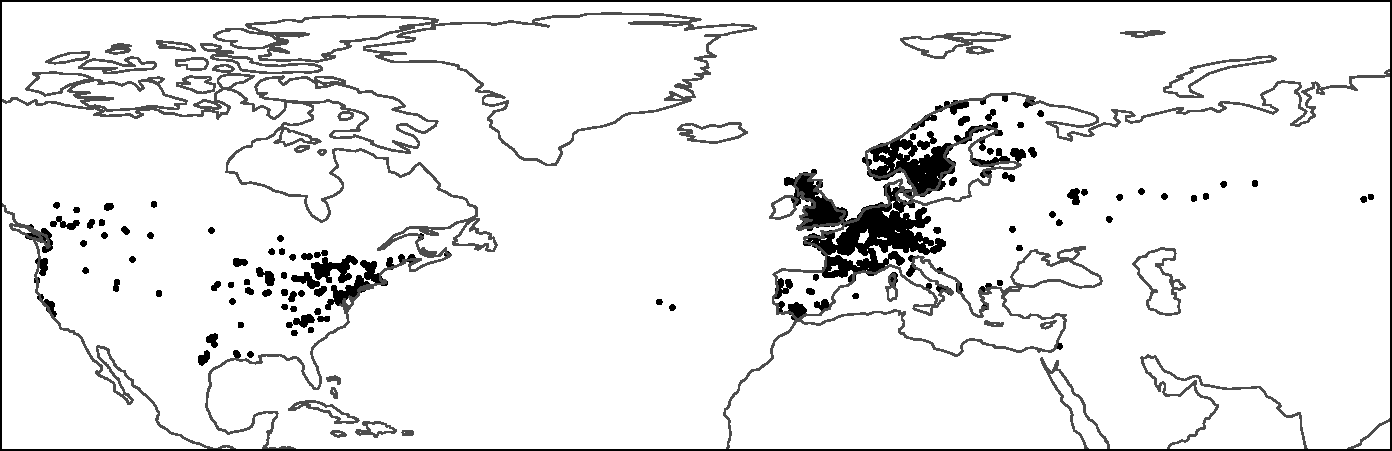
\includegraphics[width=0.9\textwidth]{Figures/Ps_presence_map.pdf}
    \caption[Training presence records for modeling the
        distribution of \textit{Philaenus spumarius.}]{\textbf{Training
            presence
            records for modeling the
            distribution of \textit{Philaenus spumarius.}}}
    \label{fig:Ps_presence_map}
\end{figure}

In addition, we randomly generated pseudo-absences, also known as
background points, using ``The Three-Step'' method proposed in
\cite{iturbide_framework_2015}. This method incorporates a model performance
criterion to determine the optimal sampling background extent, thereby ensuring
that the model fitting was not adversely affected by the pseudo-absence
sampling. Nevertheless, we accounted for the potential variability introduced
by randomly selecting points from the background by performing 10 realizations
of this sampling process. A total of 4956 pseudo-absences (three times the
number of presences) were used in each realization.

Model evaluation was performed using a $k$-fold cross-validation approach
(where $k = 10$) and the resulting AUCs (Area Under the ROC Curve) consistently
exceeded $0.9$ within the range of $0$ to $1$, with a value of $1$ indicating
perfect prediction and $0.5$ indicating no discriminatory power (i.e. random
guessing). Finally, the calibrated models were used to predict the suitability
of \textit{P. spumarius} in the reference historical period (2003-2022) and
under increasing global warming scenarios (panels b, d, f, h in
\cref{fig:Xf_Ps_suitability_change}).

\subsection{Risk velocity}

To assess the dynamic nature of the risk index and its spatial propagation,
we introduced the concept of risk velocity, a metric analogous to the recently
proposed concept of climatic velocity \cite{Loarie2009}. The risk velocity
represents the rate at which the risk index changes over time and spreads
across different locations. From an epidemiological perspective, risk velocity
can be thought as the speed and direction the host would need to move to
maintain its current risk conditions under climate change. Risk velocities were
defined following the definition of climate velocity, as the ratio of the risk
temporal trend and the risk spatial gradient in each cell. Thus, the units for
the risk velocity correspond to kilometres per year ($km/\mathrm{year}$). Risk
velocities were computed using the VoCC R package \cite{VoCC, VoCC_paper}.

\section{Results}

\subsection{Present and future climate suitability for \textit{Xylella
        fastidiosa} (PD) and \textit{Philaenus spumarius}}

To gain a deeper understanding of how climate change affects each component
of the pathosystem, we performed a separate analysis of climatic suitability
conditions for \xf{} and \textit{P. spumarius}. The thermal dependence of \xf{}
growth and survival within the infected vine was mechanistically modeled by
probability functions relating the accumulation of modified degree days
($MGDD$) and cold degree days ($CDD$) to symptom development and recovery,
$\mathcal{F}(MGDD)$ and $\mathcal{G}(CDD)$, respectively (see Methods).
Climatic suitability for pathogen establishment was then determined by
$\mathcal{F}(MGDD)\cdot\mathcal{G}(CDD)$, i.e. the overall probability of
symptom development during the growing season and subsequent survival for
overwintering infection (see Methods).	For \textit{P. spumarius}, climatic
suitability was modeled using an SDM based on a previous study
\cite{Godefroid2022_vector}, with the climatic moisture index
\cite{willmott_more_1992} and spring maximum temperatures  as key predictors
(see Methods). Both analyses were evaluated under current (2003-2022) and
future climate conditions considering scenarios of increasing global warming
(+1.5ºC, +2ºC, +3ºC, and +4ºC) based on the latest generation of regional
climate projections covering Europe \cite{jacob_regional_2020} (see Methods).

Progressive global warming increases the accumulation of MGDD during the
growing season and reduces the recovery rate (i.e. CDD) during winter, thus
favouring the geographic expansion of the pathogen
(\cref{fig:Xf_Ps_suitability_change} and \cref{fig:Xf_Ps_suitability}).
Conversely, increasing temperatures tend to reduce the climatic suitability of
vectors in more arid areas of southern Europe leading to a progressive
migration to higher areas and latitudes in continental regions in search of
climatic refuge. These general trends hold for both organisms under the +2, +3
and +4 ºC temperature increase scenarios
(\cref{fig:Xf_Ps_suitability_change}).

The mechanistic approach to modelling pathogen establishment risk enables
each of the two opposing directional processes of growth and survival (MGDD vs.
CDD) to be appropriately weighted in the final result. For example, the
Bordeaux region in western France has not been at risk due to low cumulative
MGDD and low winter protection effect.	In the transition from the +1.5ºC
scenario to the +4ºC scenario, this area will experience a spectacular increase
in risk mainly due to the expected summer warming
(\cref{fig:Xf_suitability_explainability}). Conversely, areas of Central
Europe such as Hungary and Serbia already experience suitable conditions for
pathogen growth in a +1.5ºC scenario ($\mathcal{F}(MGDD) > 0.6$); however, cold
winters tend to eliminate any potential summer infection $[\mathcal{G}(CDD) <
            0.3]$ (\cref{fig:Xf_suitability_explainability}). Climate change
would further
increase the growth of the pathogen  and reduce the winter curing effect in
Central Europe, ultimately exposing the region to \xf{}
(\cref{fig:Xf_suitability_explainability}).

\begin{figure*}[t!]
    \centering

    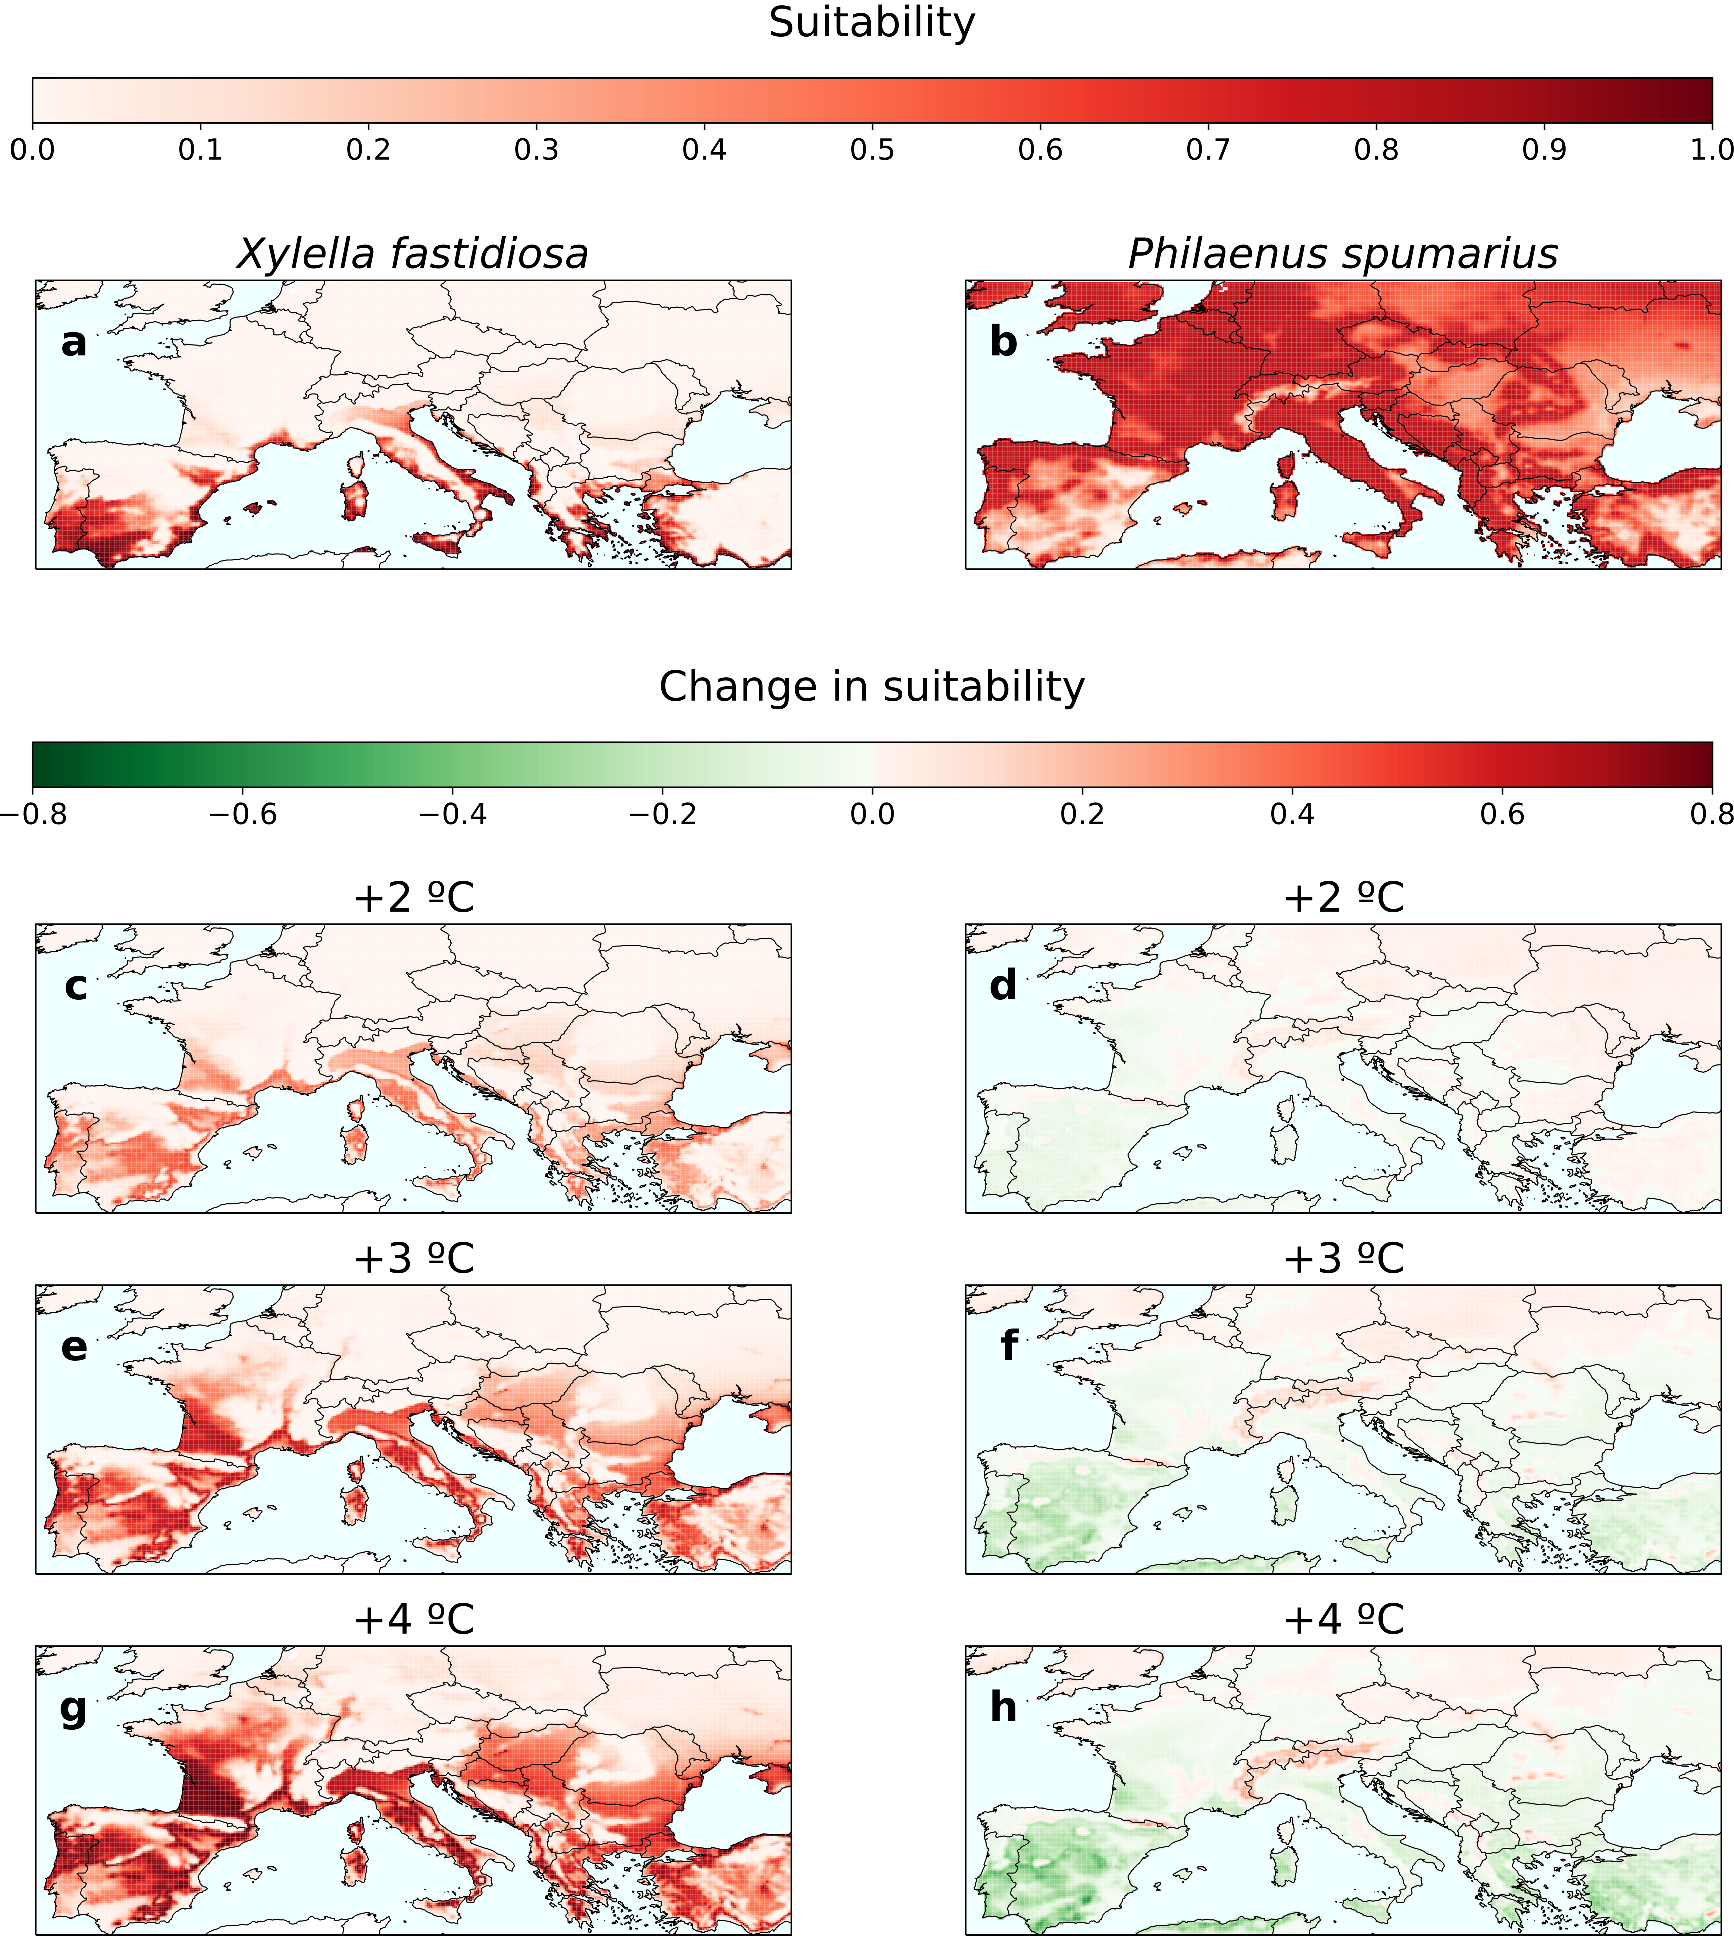
\includegraphics[width=\textwidth]{Figures/Xf_Ps_suitability_differences.pdf}
    \caption[Changes in \xf{} and \textit{P. spumarius} climatic
        suitability under different climate projections]{\textbf{Changes in
            \xf{}
            and \textit{P. spumarius} climatic
            suitability (i.e. probability of occurrence) under different
            climate
            projections compared to the current scenario (2003-2022).} Current
        climatic
        suitability for the pathogen (a) and the vector (b). In an increasing
        temperature scenario (+2ºC , +3ºC and +4ºC) the climatic suitability
        for the
        pathogen geographically expands in southern Europe and moves northwards
        (c, e
        and g) while the climatic suitability for the vector decreases (d, f
        and h).
        The suitability values for each scenario correspond to a 20-year
        average.}
    \label{fig:Xf_Ps_suitability_change}
\end{figure*}

\subsection{Pierce's disease risk projections under climate change}

The limited intersection between the climatic suitability ranges for the
pathogen and the vector (\cref{fig:Xf_Ps_suitability_change}a and b) suggests
a marginal  risk of PD epidemics in Europe. Since disease transmission requires
a vector, the climate-suitability maps for \textit{P. spumarius}  indicate a
lower risk and potential economic impact of \textit{X. fastidiosa}-induced
diseases on any host in southern Europe, particularly Spain, than previously
predicted \cite{Schneider2020}. Realistic risk maps require a defined
epidemiological framework to account for inter-annual climate variation and
transmission in disease dynamics, in addition to accounting for changes in the
distribution of climatic conditions favorable to the pathogen and vector (i.e.
climatic suitability). Our epidemic risk model focuses on delimiting the
disease dynamics by simulating an epidemic process in which the emergence of
newly exposed hosts is influenced by the climatic suitability of the vector,
while the transition to the infectious state is driven by the climatic
suitability for \xf{} chronic infections. The effective growth rate of the
infected host population over the simulated period is used to derive a risk
index $r$, bounded between $-1$ and $1$. Within this modeling framework,
different risk categories naturally emerge: no
risk ($r<-0.1$), transition zone ($-0.1\leq r<0.1$), low risk ($0.1\leq
    r<0.33$), moderate risk ($0.33\leq r<0.66$) and high risk ($r\geq0.66$).
For further details see the Methods section and the original paper
\cite{GimenezRomero2022_CommsBio}.

\begin{figure*}[t!]
    \centering
    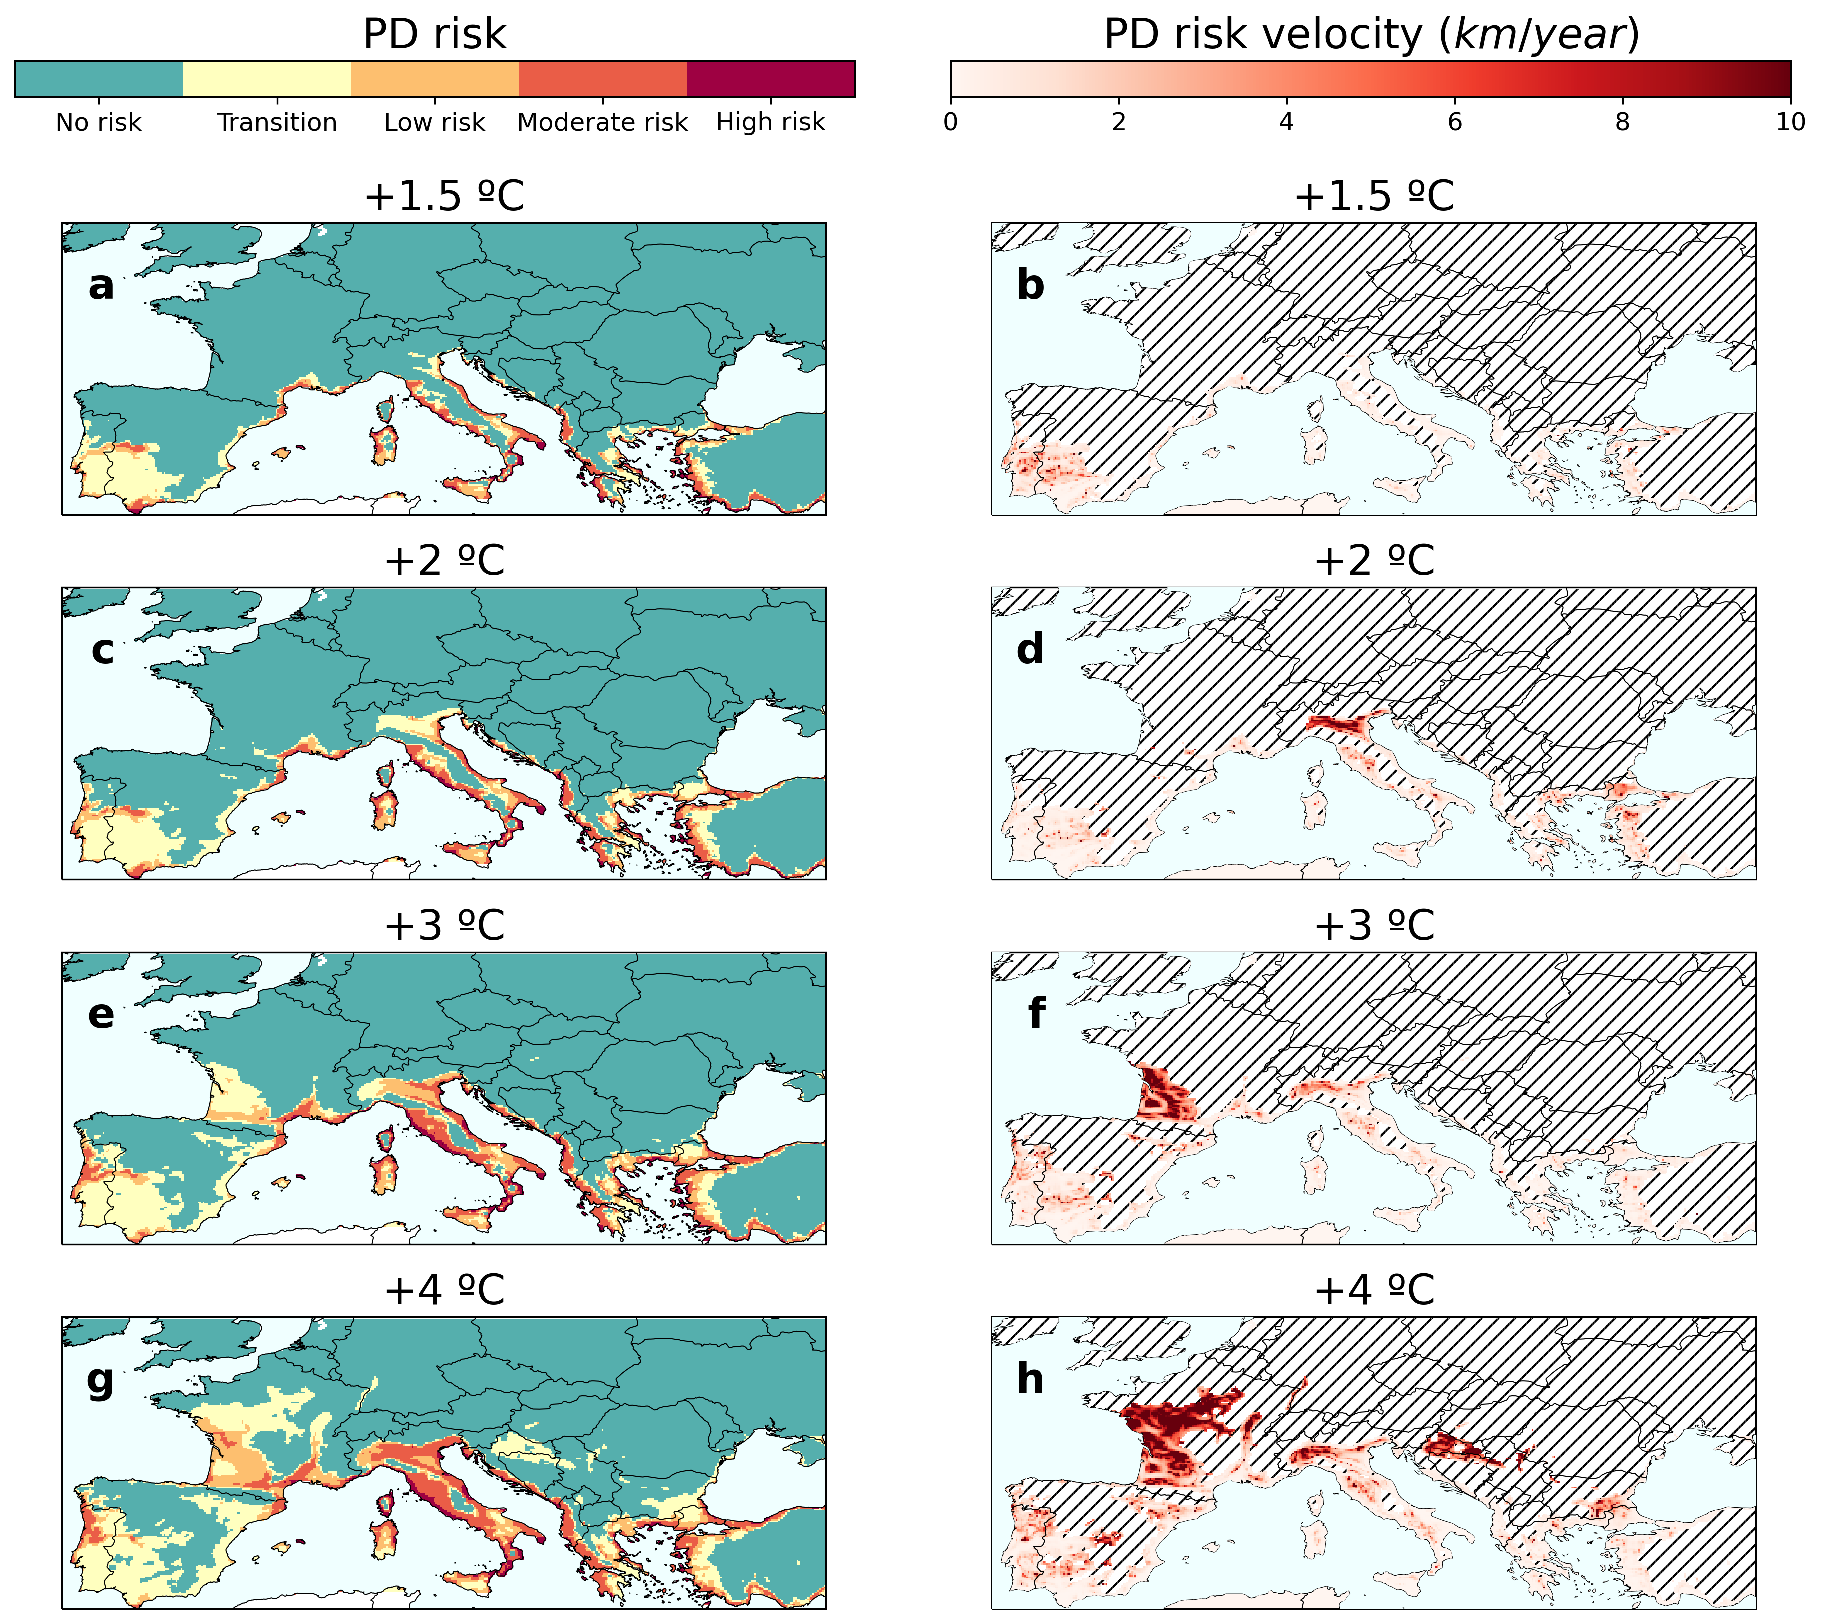
\includegraphics[width=1\textwidth]{Figures/Future_risk_PD.pdf}
    \caption[PD risk maps and associated risk velocities under
        different climate projections]{\textbf{PD risk maps and associated risk
            velocities under
            different climate projections.} (a,b) +1.5ºC climate projection.
        (c,d) +2ºC
        climate projection. (e,f) +3ºC climate projection. (g,h) +4ºC climate
        projection. Risk velocities have been calculated only in  risk zones,
        $r > 0$,
        in each scenario. Hatched lines in panels (b,d,f,h) indicate no risk
        zones
        where risk velocities have not been calculated.}
    \label{fig:PD_future_risk_zones}
\end{figure*}

Global warming (+1.5ºC, +2ºC, +3ºC, and +4ºC) is expected to increase the
risk of PD epidemics in southern Europe, with France, Italy and Portugal being
particularly affected (\cref{fig:PD_future_risk_zones} and
\cref{fig:PD_future_risk}). This general trend affects each of the risk
categories under the different climate change scenarios
(\cref{fig:PD_future_risk_velocity}). Furthermore, we observed that a global
temperature increase above +3ºC represents a tipping point for the possible
spread of PD beyond the Mediterranean (\cref{fig:PD_future_risk_zones} and
\cref{fig:PD_future_risk}). To quantify the potential spread of PD, we
calculated risk velocity, an index that allows us to identify areas where risk
is changing  or spreading rapidly (see Methods). We found a consistent and
notable increase in the mean risk velocity within most of the identified risk
zones (\cref{fig:PD_future_risk_zones} and \cref{fig:PD_future_risk_velocity}),
increasing from almost 1 km y$^{-1}$ to 5
km y$^{-1}$ as the temperature rises from a +1.5ºC to a +4ºC scenario
(\cref{tab:risk_vel}). This acceleration is evident when we
compare that in
the +1.5ºC scenario, approximately 6\% of the grid cells have risk velocities
greater than 5 km y$^{\mathrm{-1}}$, while this value increases to 50\% in the
+4ºC scenario (\cref{tab:risk_vel}). Furthermore, our estimates of
PD risk
velocity are broadly consistent with estimates of the velocity of temperature
change \cite{Loarie2009}, indicating that shifts in PD risk in our model
adequately track climate change.

\begin{figure*}[t!]
    \centering
    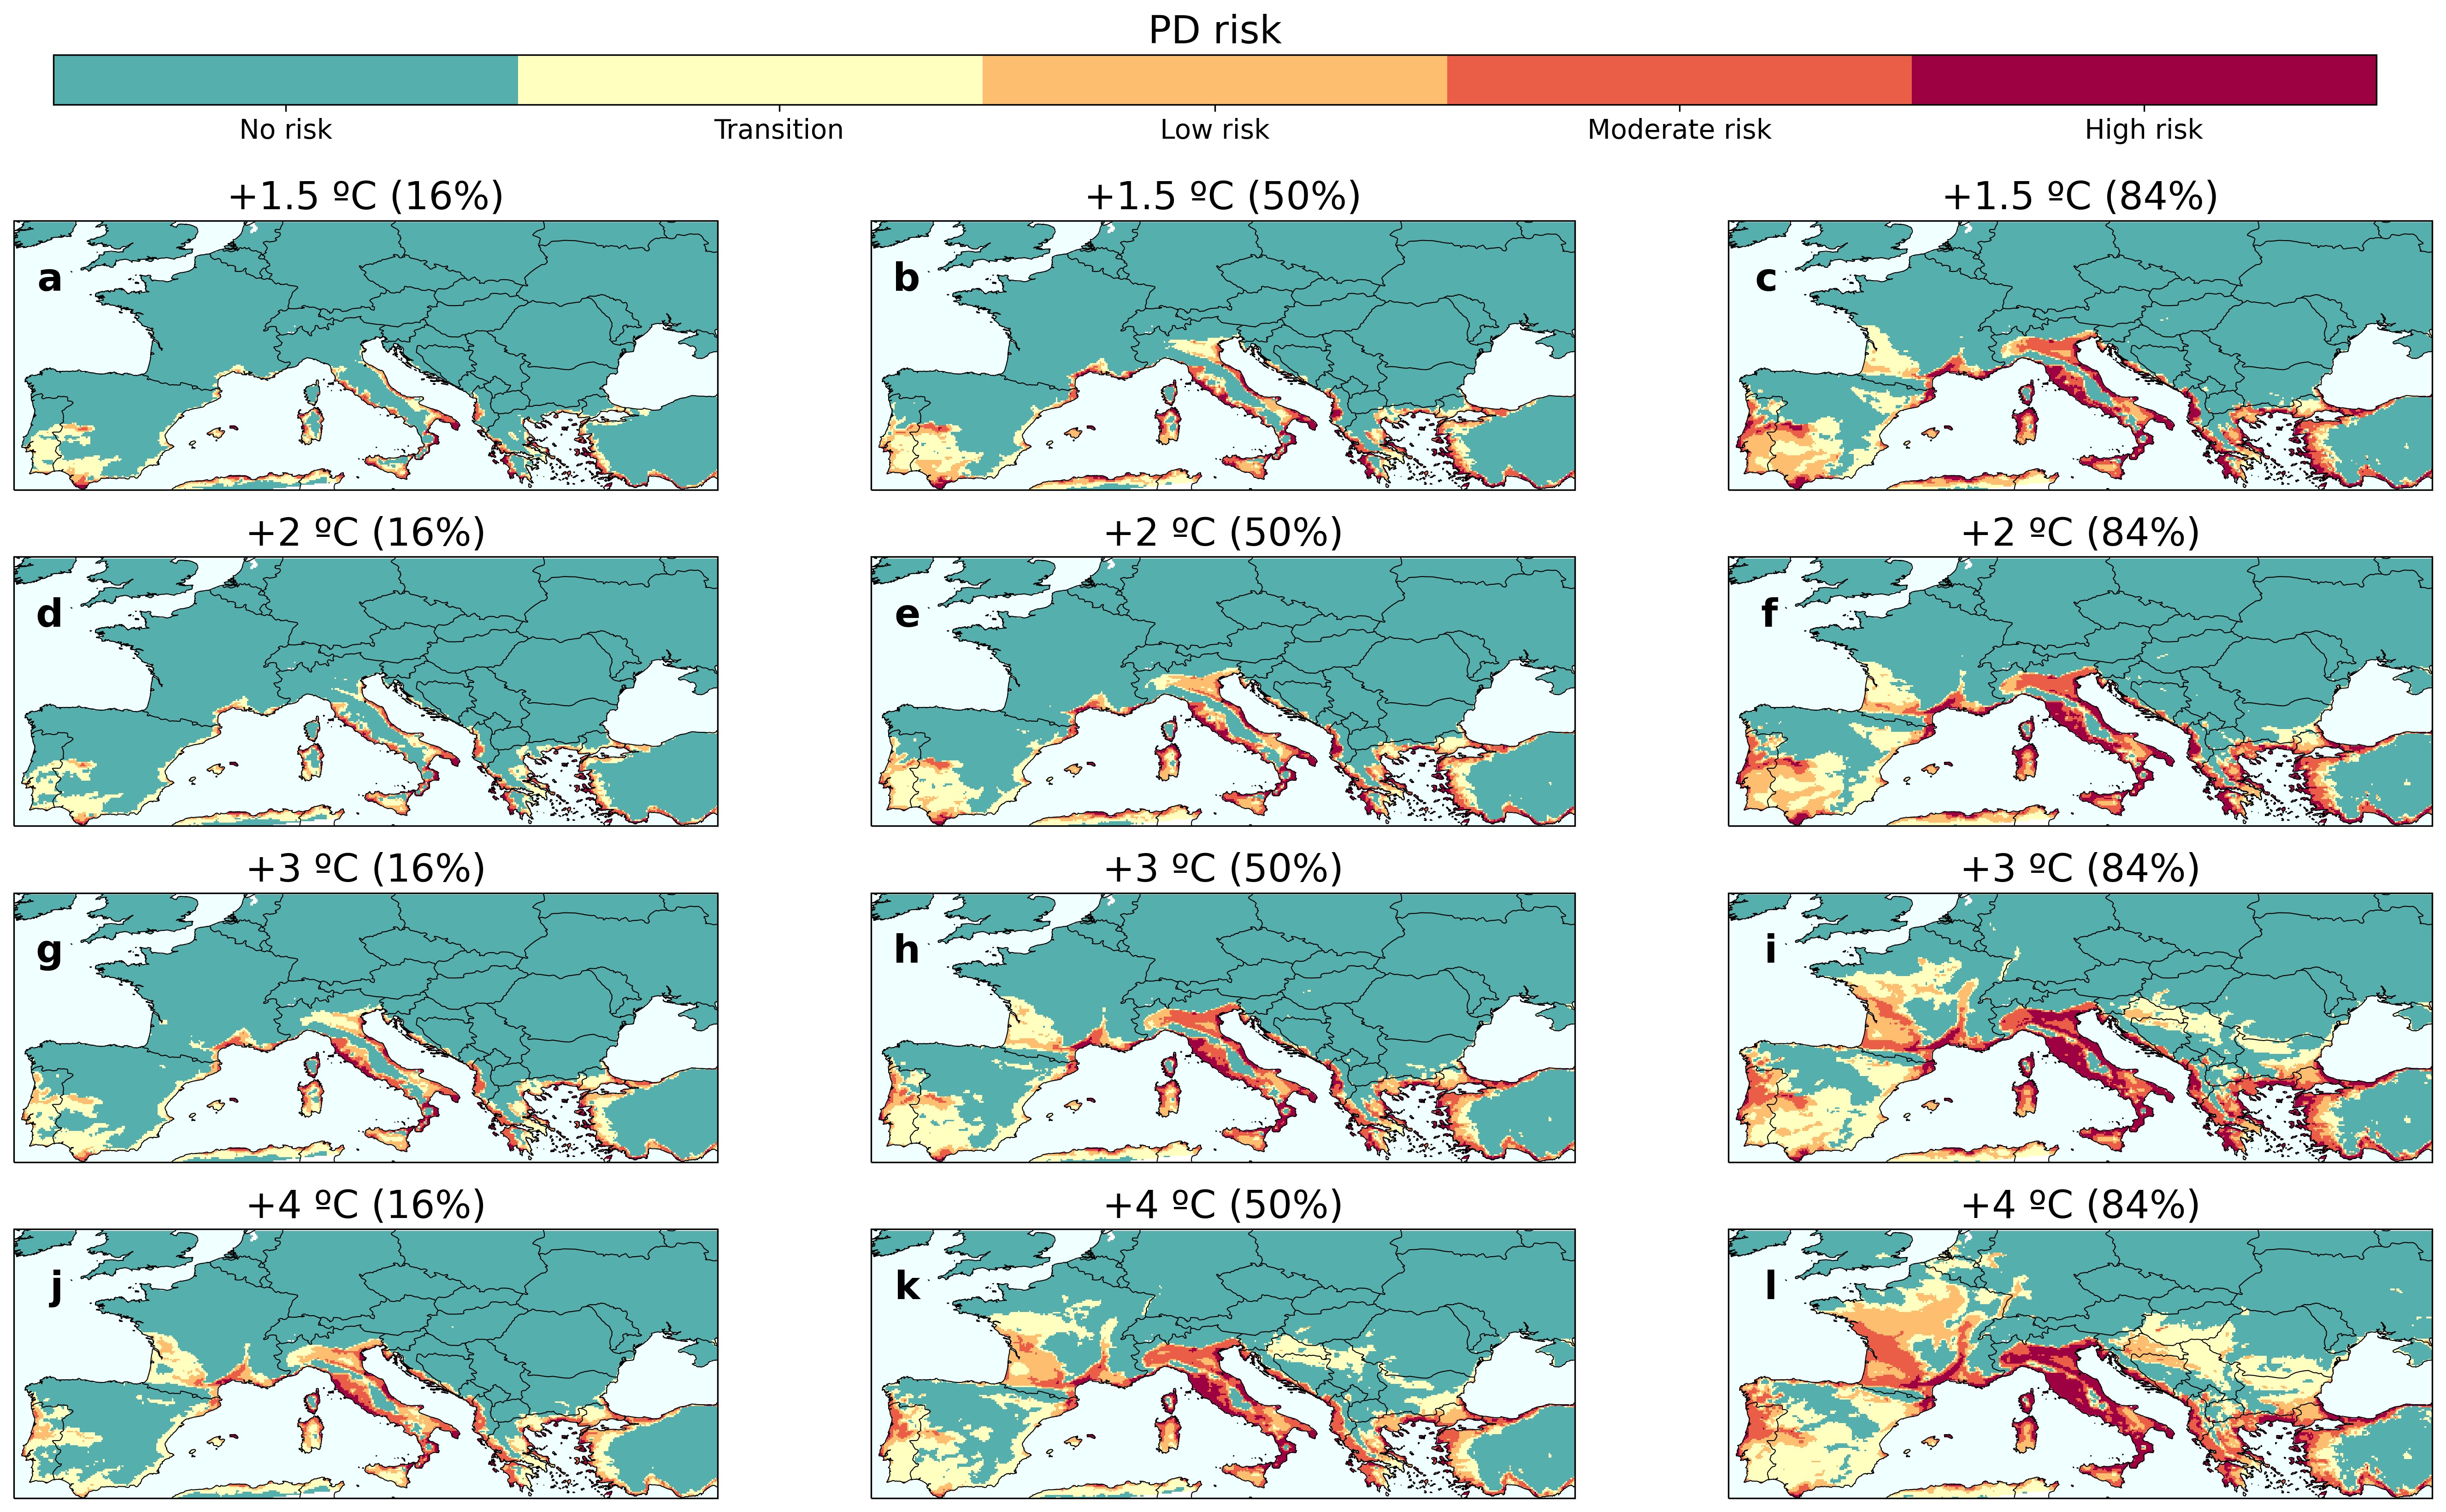
\includegraphics[width=\textwidth]{Figures/Uncertainty.png}
    \caption[Uncertainty in PD risk projections for climate change
        warming levels]{\textbf{Uncertainty in PD risk projections for climate
            change
            warming levels}. The maps show the result of the median risk values
        of the set
        of 40 regional climate model projections for each level of temperature
        increase
        (b, e, h, k) and the uncertainty of the projections considering the $1
            \sigma$
        deviations from the median, this is, the 16\% (a, d, g, j) and 84\% (c,
        f, i,
        l) percentiles. For each warming level (each row), the projected risk
        of PD is
        comprised between the results shown in the 16\% percentile (first
        column) and
        those shown in the 84\% percentile (last column) with 68\% probability
        (1$\sigma$).}
    \label{fig:uncertainty}
\end{figure*}

\cref{fig:uncertainty} shows the uncertainty in the projections of the PD
risk map, comparing the 16th and 84th percentiles ($1\sigma$) from the set of
40 regional climate models to the median risk map. The spatial distribution of
PD risk is robust across models, while the uncertainty in the level of warming
is bounded by a $\pm$ 1ºC increase (\cref{fig:uncertainty}), e.g. the median
spatial distribution of risk obtained for a +3ºC warming level is expected to
occur between the +2ºC and the +4ºC scenarios under a 1$\sigma$ confidence
level. This means that, depending on the specific model, a given spatial
distribution of risk (e.g., \cref{fig:uncertainty} h) may manifest under a +4°C
warming scenario in more conservative projections or a +2°C warming scenario in
others, while most models project it for a +3°C warming level. This indicates a
high degree of confidence in the location and projected severity of future
outbreaks, but greater uncertainty in their timing.

In order to improve the accuracy of the risk maps and the  relative impact
of PD, we carried out a comprehensive analysis at multiple scales, from the
national level to the regions with Protected Designation of Origin (PDO) and
finally taking into account the distribution of vineyards. This approach allows
us to disaggregate the results at different administrative levels to facilitate
the design of risk management and the implementation of appropriate
phytosanitary measures.

\begin{figure*}[t!]
    \centering

    \includegraphics[width=\textwidth]{Figures/Future_risk_country_and_vineyards.pdf}
    \caption[Multi-scale spatial analysis of PD future risk in
        Europe]{\textbf{Multi-scale spatial analysis of PD future risk in
            Europe.} (a, c, e, g) Percentage of country areas at risk ($r>0.1$)
        for each
        climate projection. (b, d, f, h) PD risk zones in Protected Designation
        of
        Origin (PDO) wine regions for each climate projection. PDO data was
        obtained
        from \cite{Candiago2022}. The corresponding interactive analysis at the
        vineyard level can be found in \cite{Webpage}}
    \label{fig:vineyards}
\end{figure*}

Overall, our model simulations show a consistent
increasing trend in the risk of PD in Europe under all climate change
scenarios. The percentage of land area at risk in Europe increases from 0.32\%
in the +1.5ºC scenario to 1.87\% in the +4ºC, while the number of regions with
PDO at risk increases from 18.17\% to 47.32\% . The vineyard area  increases
from 18.67\% to 40.35\% (\cref{tab:general}). At country level
Portugal and
Greece face the highest overall risk, escalating from 12\% and 2\% of their
area  in the +1.5ºC scenario to a striking 47\% and 63\%  respectively in a
+4ºC scenario. In contrast, countries such as France and Italy experience a
smaller but still significant increase in risk area, never exceeding the 20\%
threshold, while Spain, the third largest wine producer, shows a decreasing
trend in risk areas above the +2ºC scenario (\cref{fig:vineyards} and
\cref{tab:countries}). Such contrasting patterns in PD risk between
countries
only emerge when using our modelling framework.

A different picture emerges when looking at the spatial distribution of PDO
regions and vineyards. For example, PD risk within French and Italian PDO
regions increases significantly from 13.4\% and 45.8\% in a +1.5ºC scenario to
41.6\% and 82.7\% in a +4ºC scenario (\cref{fig:vineyards} and
\cref{tab:countries}), while the percentage of vineyard area at
risk rises
from 24.21\% and 57.49\% in a +1.5ºC scenario to an astonishing 80\% in a +4ºC
scenario. Important European PDOs would be at risk from a warming of  +2ºC,
such as parts of the southern Rhône Valley (Châteneuf du Pape), Provence and
Languedoc in France, Penedés in Spain, Bairrada in Portugal, and Chianti and
Brunello di Montalcino among others in Italy (see Supplementary Information). A
detailed interactive analysis of the impact of PD in European PDO regions and
vineyards is available on our website \cite{Webpage}.

\section{Discussion}

Previous research has attempted to assess the potential geographic
distribution of  \xf{} subspecies, the insect vector \textit{P. spumarius} and
PD using species distribution models (SDMs) under future climates. While these
climate-suitability-based predictions provide insights into the ecological
niche of key disease players, bioclimatic correlative models neglect disease
dynamics, a key factor in avoiding disease overestimation
\cite{GimenezRomero2022_CommsBio}. Unlike previous attempts, our approach
integrates
the compound effect of climate change in the pathosystem using a mechanistic
epidemiological model to overcome these limitations.  Unlike dimensionless
climatic suitability indexes or disease probabilities used in SDMs, the risk
index, $r$, in our model provides information on the expected growth rate in
the event of an outbreak . Furthermore, the risk index is not fixed but varies
annually depending on the weather conditions of the previous years.
Inter-annual climate variability thus has an impact on disease dynamics,
especially in areas where the risk index is lower.  Another feature of our risk
predictions is their lack of ambiguity, which should not be confused with
certainty. Risk estimates are based on $R_0$, which depends on the insect
vector population \cite{GimenezRomero2022_PRE}, among other factors. Areas
where
$r<-0.1$ permanently cannot theoretically support an outbreak, and the
population of infected plants will decline over time. For example, our model
clearly indicates that there is no risk of PD in the UK. This is not an
arbitrary threshold; it  is given by the epidemiological model.  It is
therefore very likely that the absence of PD in continental Europe is a
consequence of low risk indices and that it has only become established in
certain coastal areas since the late 1990s. On the contrary, the risk index in
the Mediterranean islands has remained moderately high with little variation
over the last 40 years \cite{GimenezRomero2022_CommsBio}.

Because Pierce's disease has only affected vineyards on the island of
Mallorca \cite{moralejo2019insights}, little attention has been paid to the
risk of it reaching continental vineyards. Our risk model indicates why this
possibility was very low until the mid-90s, and what the conditions were for it
to occur on the Mediterranean islands \cite{GimenezRomero2022_CommsBio}.  In
this work,
we clearly show that  with increasing temperatures PD will become a serious
threat to important wine-growing areas in southern Europe that were not
previously at risk. A key finding of our study is the identification of a
tipping point for the risk of PD establishment at a global mean temperature
increase of +3ºC. Beyond this threshold, the risk of PD spreading north of the
Mediterranean region becomes remarkably higher, while the risk of PD epidemics
in Portugal, Italy and France (\cref{fig:PD_future_risk_zones}) undergoes a
significant quantitative leap. This suggests that as global temperatures
continue to rise, the range of PD may expand into new territories. Indeed, the
projected increase in risk velocities under higher warming scenarios further
emphasizes the potential for rapid spread of PD into previously unaffected
regions (\cref{fig:PD_future_risk_zones}).

Pest risk map projections are subject to uncertainties inherent in the
variability of climate model predictions \cite{venette2010pest}. While previous
studies on pathogen and vector distributions have been based on a limited
number of climate models, our risk maps are based on the most modern set of
regional climate projections produced by the EURO-CORDEX initiative, reflecting
the state-of-the-art knowledge (\cref{tab:GCM-RCM}). This allows us to
adequately estimate the uncertainty of the resulting PD risk map projections
for each temperature rise scenario. This confirms that although the spatial
distribution of the risk of establishment is robust, there is an uncertainty of
$\pm$ 1ºC in the level of warming (\cref{fig:uncertainty}). The models are
therefore fairly good at  pointing  where the increased risk will occur, but it
is more difficult to know when it will be reached.

Overall, our results highlight the contrasting effect of climate change on
PD risk distribution in Europe, revealing it as a multi-factor and multi-scale
process (\cref{tab:countries}). Climate change has an opposite effect on each
component of the pathosystem, enhancing areas of potential chronic PD
infections while diminishing the suitable geographic range for the vector. At
the same time, the characteristic spatial scale at which risk is assessed
strongly influences conclusions. At the country level, there are significant
variations in the extent of accumulated risk between different projections.
However, when analyzed at a finer scale, such as at the level of PDO regions or
vineyards, the results change completely. Countries that previously had
marginal areas at risk now show a higher percentage of PDO regions and vineyard
at risk. These results underlie the urgency of tailored mitigation and
adaptation strategies to protect vineyards and PDOs, considering their specific
spatial distribution and risk index, as well as the potential impacts of
climate change.

Our results are influenced by the intrinsic uncertainty associated with the
correlative models used to determine the spatial distribution of the vector,
the epidemiological parameters, and the uncertainties in the climatic
projections. Although the spatial resolution of our climate projections is
considered to be high, it may not capture the complex micro-climate structure
found in certain European wine-producing regions. Therefore, risk assessment
results could differ locally with higher-resolution data. In addition, we have
not considered the possible influence of climate change on latitudinal and
altitudinal shifts in the distribution of European vineyards
\cite{hannah2013climate,moriondo2013projected}, as this would only affect the
calculation of the percentage of vineyard surface at risk but not the actual
spatial distribution of risk. In any case, the risk estimates for the PDO
regions include areas much larger than the areas of planted vines, which allows
some margin in the adaptation and migration of the vineyards to different
micro-climatic conditions. In addition, the PDO and vineyard databases used in
this study are also have their own limitations. Future studies incorporating
more refined modeling techniques, specific regional grapevine varieties, crop
management and improved data resolution would enable a more nuanced
understanding of PD risk and its potential impact at the local scale.

It is noteworthy that the mathematical framework employed in this study
could be applied to other \textit{Xylella fastidiosa} diseases, such as Almond
Leaf Scorch Disease or Olive Quick Decline Syndrome and, more generally, to
other vector-borne plant diseases. However, this requires the availability of
some specific data and conducting some experiments. First, data for the
temperature-dependent growth rate of the pathogen is needed to build the
function that computes the MGDD. Then, symptom development experiments need to
be carried out to build the $\mathcal{F}(MGDD)$ and $\mathcal{G}(CDD)$
functions that relate symptom development with temperature. Finally, the
spatial distribution of the agent responsible for disease transmission is
desired. Of course, using presence/absence data one can use SDM to obtain this
spatial distribution.

Climate change is currently one of the biggest challenges for EU
agricultural policy \cite{fellmann2018major}. Quantitative regional predictions
of climate change on emerging diseases, such as this one, provide a valuable
and unambiguous tool for decision-making. In our approach to the problem, risk
indexes not only include information on where or where not PD may become
established, but also reflect the exponential growth rate of potential
epidemics, which are directly related to their potential economic impact. In
addition, risk indices and velocities provide a dynamic framework for assessing
the feasibility of eradication efforts when \xf{} is detected in a new area,
providing critical information for strategic crop protection. Our study
evidences the need to selectively allocate more resources to surveillance and
research on PD in southern European countries, considering the associated
uncertainties. This strategic allocation of resources based on risk assessment
can help to prioritise proactive measures and effectively manage the potential
impact of PD in different European countries.

Our research highlights the complex dynamics of PD and its relationship
with climate change. By adopting an interdisciplinary approach that integrates
climate projections, epidemiological modelling, and spatial analysis, we
provide valuable insights into the potential establishment and spread of PD in
European wine-growing regions from the country to the vineyard levels. Our
study demonstrates that an accurate assessment of the risk of PD establishment
requires a nuanced understanding of the vector-plant-pathogen-climate system
and the explicit consideration of the vineyard spatial setting. These findings
can inform decision-making processes and support the development of effective
strategies to mitigate the risks posed by PD and safeguard the future of
viticulture in the face of a changing climate.\label{ch:xf_climate_change}

%----------------------------------------------------------------------------------------
%	High-resolution climate data reveals increased risk of Pierce's Disease for 
%   grapevines worldwide	
%----------------------------------------------------------------------------------------
\chapterimage{ribeira-sacra.jpg}
\chapterspaceabove{6.75cm}
\chapterspacebelow{7.25cm}

\chapter{Pierce's Disease risk with high-resolution climate data}
\vspace{1cm}

\textbf{Àlex Giménez-Romero$^{1}$, Eduardo Moralejo$^{2}$, Manuel A.
    Matías$^{1}$}

\vspace{1cm}

\begin{enumerate}
    \small
    \item Instituto de Física Interdisciplinar y Sistemas Complejos, IFISC
          (CSIC-UIB), Palma de Mallorca 07122, Spain
    \item Tragsa, Passatge Cala Figuera 6, 07009 Palma de Mallorca, Spain
\end{enumerate}

\vspace{1cm}

\textbf{Published as}

\vspace{0.5cm}

\fullcite{GimenezRomero2024}

\newpage
\section{Introduction}

Climate plays a pivotal role in shaping the distribution and dynamics of
agricultural pests and pathogens
\cite{Harvell2002,Lafferty2009,Bebber2013,Bebber2014,Delgado-Baquerizo2020},
with implications for global food security \cite{Fones2020, Ristaino}. As our
climate undergoes unprecedented changes due to anthropogenic activities,
agriculture faces multifaceted threats ranging from alterations in temperature
and precipitation patterns to increased frequency of extreme weather events
\cite{skendzic2021impact}. Such shifts create novel environments that may
favour the proliferation of certain pests or pathogens while posing challenges
to the survival of others \cite{Bebber2013, Dudney2021}. The consequences of
these changes extend beyond immediate agricultural landscapes, reverberating
through global food systems and posing significant challenges to the
sustainability and resilience of food production \cite{Ortiz-Bobea2021}.

Understanding the intricate relationships between climatic conditions, the
pathosystem components, and the subsequent epidemiological dynamics is
essential for developing effective strategies to mitigate and manage emerging
agricultural challenges, especially in the face of changing environmental
conditions. However, modelling disease epidemics is a complex task , as they
are emergent phenomena resulting from non-linear interactions between disease
components that also exhibit non-linear responses to changes in environmental
variables \cite{scherm1994global,garrett2011complexity,jeger2019epidemiology}.
Thus, while climate primarily determines the potential geographic range of each
organism in the pathosystem, the development of epidemic outbreaks depends on
favourable host-pathogen-vector-climate interactions that drive transmission
chains.

It has long  been recognised that ecological phenomena typically depend on
the scale of description,  particularly with regard to the effects of climate
\cite{Levin1992}. Climatic databases with finer spatial resolution are
continuously being developed with the goal of allowing more accurate
predictions \cite{Navarro-Racines2020}.  Some recent studies have shown that
the local climate experienced by individuals might deviate substantially from
regional averages, with implications for the population dynamics of a forest
herb \cite{Christiansen2024}. Likewise, the choice of climate data affects the
predictions of species distribution models (SDMs) \cite{Abdulwahab2022}. In
particular, the spatial resolution of the data can influence the predictions of
invasion risk for some species \cite{Dubos2023}.  It is therefore clear that
the resolution of climate data will have a significant impact on predicting the
risk of plant diseases and pests.

Among emerging pathogens \textit{Xylella fastidiosa} (Xf) is considered one
of the most dangerous phytopathogenic bacteria worldwide
\cite{Hopkins2002,EFSA_xf}. It is naturally transmitted by xylem sap-feeding
insects, such as sharpshooters and spittlebugs, and exhibits a broad host range
that encompasses economically important crops such as grapevines, citrus,
almonds and olive trees \cite{redak2004biology,EFSA_xf}. The consequences of Xf
diseases are devastating: about 200 million citrus trees are  infected annually
in Brazil \cite{Lindow2019}, there are	loses over \$100 million annually in
the grape industry in California  \cite{tumber2014pierce} and approximately
$21$ million olive trees have been killed by the bacterium on the Apulia region
in Italy  \cite{Sabelli2023}. Assuming massive spread throughout Europe, Xf has
been projected to potentially contribute up to \texteuro5.2 billion of annual
losses in the olive sector alone \cite{Schneider2020}. Overall, Xf diseases
pose a major threat to agrosystems worldwide, highlighting the need for precise
and predictive models to guide effective management practices.

Previous research has provided insights into the potential geographic range
of  Xf subspecies through SDMs \cite{Bosso2016b, Godefroid2022}. These models,
however, have led to overestimates of risk by failing to account for the
distribution and abundance of potential vectors necessary for disease
transmission  \cite{Godefroid2022_vector}.  A quite different approach to
mapping PD risk has been developed based on climate-driven epidemiological
models with the option to integrate vector's distribution information and the
specificity of the Xf  subsp. \textit{fastidiosa} strain responsible for PD
(hereafter \xf{}) \cite{GimenezRomero2022_CommsBio}. This model correctly
identifies
areas in the United States with recurrent  PD outbreaks and forecasts
increasing epidemic risk in Mediterranean islands and coastlines  with ongoing
climate change.

Although risk maps based on hourly temperature data from the ERA5 have
allowed fine adjustments in the calibration of the thermal response to Xf
infection, these achievements have entailed losses in spatial resolution (0.1º
spatial resolution) \cite{GimenezRomero2022_CommsBio, munoz2019era5land}. Such
limitation is particularly significant when dealing with vector-borne plant
diseases like PD, where the interactions between the pathogen, vector, and host
plants exhibit non-linear responses to climatic conditions. Subtle variations
in temperature, humidity, or precipitation at the local scale thus can have
profound effects on the reproduction and life cycles of the organisms involved
and, hence, on the dynamics of disease transmission.

Topographical heterogeneity is a recognised issue in invasion biology, but
has received little attention in crop science.	Vineyards are increasingly
located in valleys, ridges, hillsides and riverbanks usually with altitudinal
and microclimatic gradients in short transects.  They are therefore a
remarkable example of  a crop subject to scaling problems when studying
ecological or epidemiological processes at  regional and global scales.  In
this work, we address this spatial resolution limitation by modelling the risk
of PD  using high-resolution climate data from the CHELSA dataset
\cite{Karger2017}. The study period was deliberately chosen  to include real
data on temperature increases due to ongoing climate change.  Our study shows a
greater global risk of PD and a higher rate of risk increase, underscoring the
urgency of reevaluating global strategies to prevent the spread of the pathogen
with international trade in plant diseases.

\section{Results}

\subsection{Global differences in  PD risk between coarse and fine-grain
    climate data}

We computed the risk of PD using the previously developed climate-driven
epidemiological model \cite{GimenezRomero2022_CommsBio} coupled with the CHELSA
dataset
\cite{Karger2017}, which features key climate variables (e.g. temperature and
precipitation) at a high spatial resolution of 1 km and daily temporal
resolution covering the period 1979-2016. The resulting spatial and temporal
patterns of disease risk in the main wine-growing regions were compared with
previous risk projections derived from the ERA5 dataset
\cite{munoz-sabater_era5-land_2021}, characterised by an intermediate  spatial
resolution of 10 km  and hourly temporal resolution
\cite{GimenezRomero2022_CommsBio}.
Briefly, the model simulates the initial dynamics of the disease  influenced by
climatic variables and the presence of vectors, giving rise to a risk index,
$r$, which represents the normalised growth rate of the infected population,
where $r=1$ is the maximum rate achieved at optimal climatic conditions (see
Methods). Negative risk indices project an exponential decrease of the infected
population (no risk), whereas positive values give rise to an outbreak, with
higher values accounting for major incidence and potential severity. Risk
categories  emerge naturally from this formalism as No Risk ($r\leq-0.1$)
Transition ($-0.1<r \leq0.1$), Low Risk ($0.1<r\leq0.33$), Moderate Risk
($0.33<r\leq0.66$) and High Risk ($r>0.66$). Risk projections in Europe use the
climatic suitability, $s$, of the main European vector, \textit{P. spumarius}
(see Methods), while for the rest of the world it is assumed that there are no
risk-limiting effects due to the vector  ($s=1$), but only due to climatic
conditions.

\begin{table}[H]
    \caption{Changes in Pierce's Disease Risk Zones in Different Viticulture
        Regions. The table illustrates transitions between risk and no-risk
        categories,
        as well as transitions among risk categories, highlighting the dynamic
        shifts
        in risk patterns across viticulture areas in Europe, the USA, South
        Africa,
        South America, and Australia. Risk increase refers to changes from low
        to
        moderate risk or from moderate to high risk. Likewise, risk decrease
        refers to
        changes from moderate to low risk or high to moderate risk.}
    \label{tab:risk_category_dif}
    \resizebox{\textwidth}{!}{%
        \begin{tabular}{lccccc}
            \hline
                                                 & \textbf{Europe}       &
            \textbf{USA}                         & \textbf{South Africa} &
            \textbf{South America}               & \textbf{Australia}
            \\ \hline
            \textbf{Risk to no-risk (km$^2$)}    & 1.91e+04
                                                 & 3.93e+04
                                                 & 2.26e+04
                                                 & 2.49e+05
                                                 & 5.81e+04
            \\
            \textbf{Transition to risk (km$^2$)} & 6.37e+04
                                                 & 1.37e+05
                                                 & 5.53e+04
                                                 & 3.79e+04
                                                 & 8.49e+04
            \\
            \textbf{Risk decrease (km$^2$)}      & 3.58e+04
                                                 & 1.46e+05
                                                 & 3.56e+05
                                                 & 1.76e+05
                                                 & 1.28e+06
            \\
            \textbf{Risk increase (km$^2$)}      & 6.28e+04
                                                 & 2.37e+05
                                                 & 1.05e+05
                                                 & 1.50e+05
                                                 & 1.55e+05
            \\
            \textbf{No risk to risk (km$^2$)}    & 2.04e+05
                                                 & 2.36e+05
                                                 & 2.77e+05
                                                 & 1.90e+05
                                                 & 2.15e+05
            \\
            \textbf{Total changes (km$^2$)}      & 3.85e+05
                                                 & 7.95e+05
                                                 & 8.15e+05
                                                 & 8.03e+05
                                                 & 1.79e+06
            \\ \hline
        \end{tabular}
    }
\end{table}

When contrasting model results derived from high- and medium-resolution
data for the latest available time (2016), the disparity in risk projections
extends beyond regional differences, showing a global increase in risk indices
across wine-growing areas (\cref{fig:risk_indices_dif} and
Online Supplementary Information).  Overall, these increases
(\cref{fig:risk_categories_dif}) in the extension of PD risk areas ranged from
100,000 to 1 million km$^2$ across viticulture regions worldwide. Transitions
from no-risk to risk zones covered an area one order of magnitude larger than
those in the opposite direction --from risk to no-risk
(\cref{fig:risk_categories_dif,tab:risk_category_dif}). In total, a surface of
4.6 million km-2 changed its risk category with the CHELSA database,
representing about a 16\% of the land area studied. In contrast, the largest
decreases in the risk indices occurred mainly in the Southern Hemisphere,
although with few exceptions most of these decreases remained within the risk
zones (\cref{fig:risk_indices_dif}), while similar land expansions were
observed to  increase their risk category (low to moderate or moderate to high)
(\cref{fig:risk_categories_dif,tab:risk_category_dif}). The largest changes in
risk indices occur in ecotones on both sides of the $r=0$ line, as is clearly
seen in the south-eastern United States, in coastal areas (e.g., southern
Australia and northern California) due to higher resolution that better
distinguishes between land and coast, and finally in the river valleys and
slopes of mountain systems
(\cref{fig:risk_categories_dif,tab:risk_category_dif}).

\begin{figure}[H]
    \centering
    \includegraphics[width=1\textwidth]{Figures/ERA5_vs_CHELSA_dif.pdf}
    \caption{Difference in risk projections based on CHELSA
        (high-resolution, 1 km) and ERA5 (mid-resolution 10 km) datasets in
        global
        viticulture areas. (A) Europe (B) South America (C) United States (D)
        Australia
        (E) South Africa.}
    \label{fig:risk_indices_dif}
\end{figure}

Next, we compared the temporal progression of the area at risk using both
high and mid-resolution data over the entire available time span (1986-2016),
considering that the risk for each year is computed based on the preceding
seven years. We found a notable global surge in the rate increase of the area
at risk within viticulture zones worldwide, practically doubling previous
estimates (Online Supplementary Information). These results point to an
accelerated
pace at which the risk of PD is growing, compatible with the predictions of
different global warming scenarios \cite{GimenezRomero2023_PD}.

\begin{figure}[H]
    \centering
    \includegraphics[width=\textwidth]{Figures/ERA5_vs_CHELSA_zones.pdf}
    \caption{Changes in risk categories between CHELSA (high-resolution, 1
        km) and ERA5 (mid-resolution 10 km) projections in global viticulture
        areas.
        (A) Europe (B) South America (C) United States (D) Australia (E) South
        Africa.
        Risk category increase refers to changes from low to moderate risk or
        from
        moderate to high risk. Likewise, risk category decrease refers to
        changes from
        moderate to low risk or high to moderate risk.}
    \label{fig:risk_categories_dif}
\end{figure}

\subsection{Pierce's Disease risk surges in previously unresolved
    microclimates}

River valley vineyards are renowned  for their high quality wines, such as
Douro, Napa and Rhone and many others. It is therefore important to understand
the risk of  PD with climate change at	a more detailed level. In our analysis,
we have identified rivers and valleys as specific relief areas where a greater
increase in PD risk is observed when employing CHELSA’s finer- scale climate
data (\cref{fig:microclimates}).

\begin{figure}[H]
    \centering
    \includegraphics[width=0.9\textwidth]{Figures/ERA5_vs_CHELSA_rivers.pdf}
    \caption{Effect of microclimatic conditions of rivers and valleys on
        Pierce's Disease of grapevines. Comparison of the risk predicted using
        ERA5
        mid-resolution dataset (A,C,E) and CHELSA high-resolution dataset
        (B,D,F).
        (A-B) North-western Iberian Peninsula. (C-D) Sourthern France and
        North-eastern
        Spain. (E-F) Western United States. Black dots represent grapevines
        (\textit{Vitis vinifera}) presence data obtained from GBIF (see
        Methods).}
    \label{fig:microclimates}
\end{figure}

In some important wine-growing areas of
southern Europe, we observed an abrupt emergence of risk zones previously
classified as no-risk when using lower resolution climate data
(\cref{fig:microclimates}). Such pronounced differences in risk patterns are
highlighted for example in the fairly steep valleys and hillsides along the
Douro River in Portugal, where the specific microclimatic conditions were
previously obscured by the coarser resolution of the ERA5 data. These findings
are particularly significant for PD,  as vineyards are often located in close
proximity to rivers or valleys and their surroundings, creating microclimates
that attenuate cold winters (black dots in (\cref{fig:microclimates})). A
gradual increase in the climatic suitability for PD in some river basins may
thus favour the spread of the pathogen from coastal  to interior areas of the
continents, allowing interconnection between areas that would otherwise remain
isolated. Coastal areas close to cool water masses may also undergo an increase
in risk  when using higher resolutions data, as exemplified in California
(\cref{fig:microclimates} e,f).

\begin{figure}[H]
    \centering

    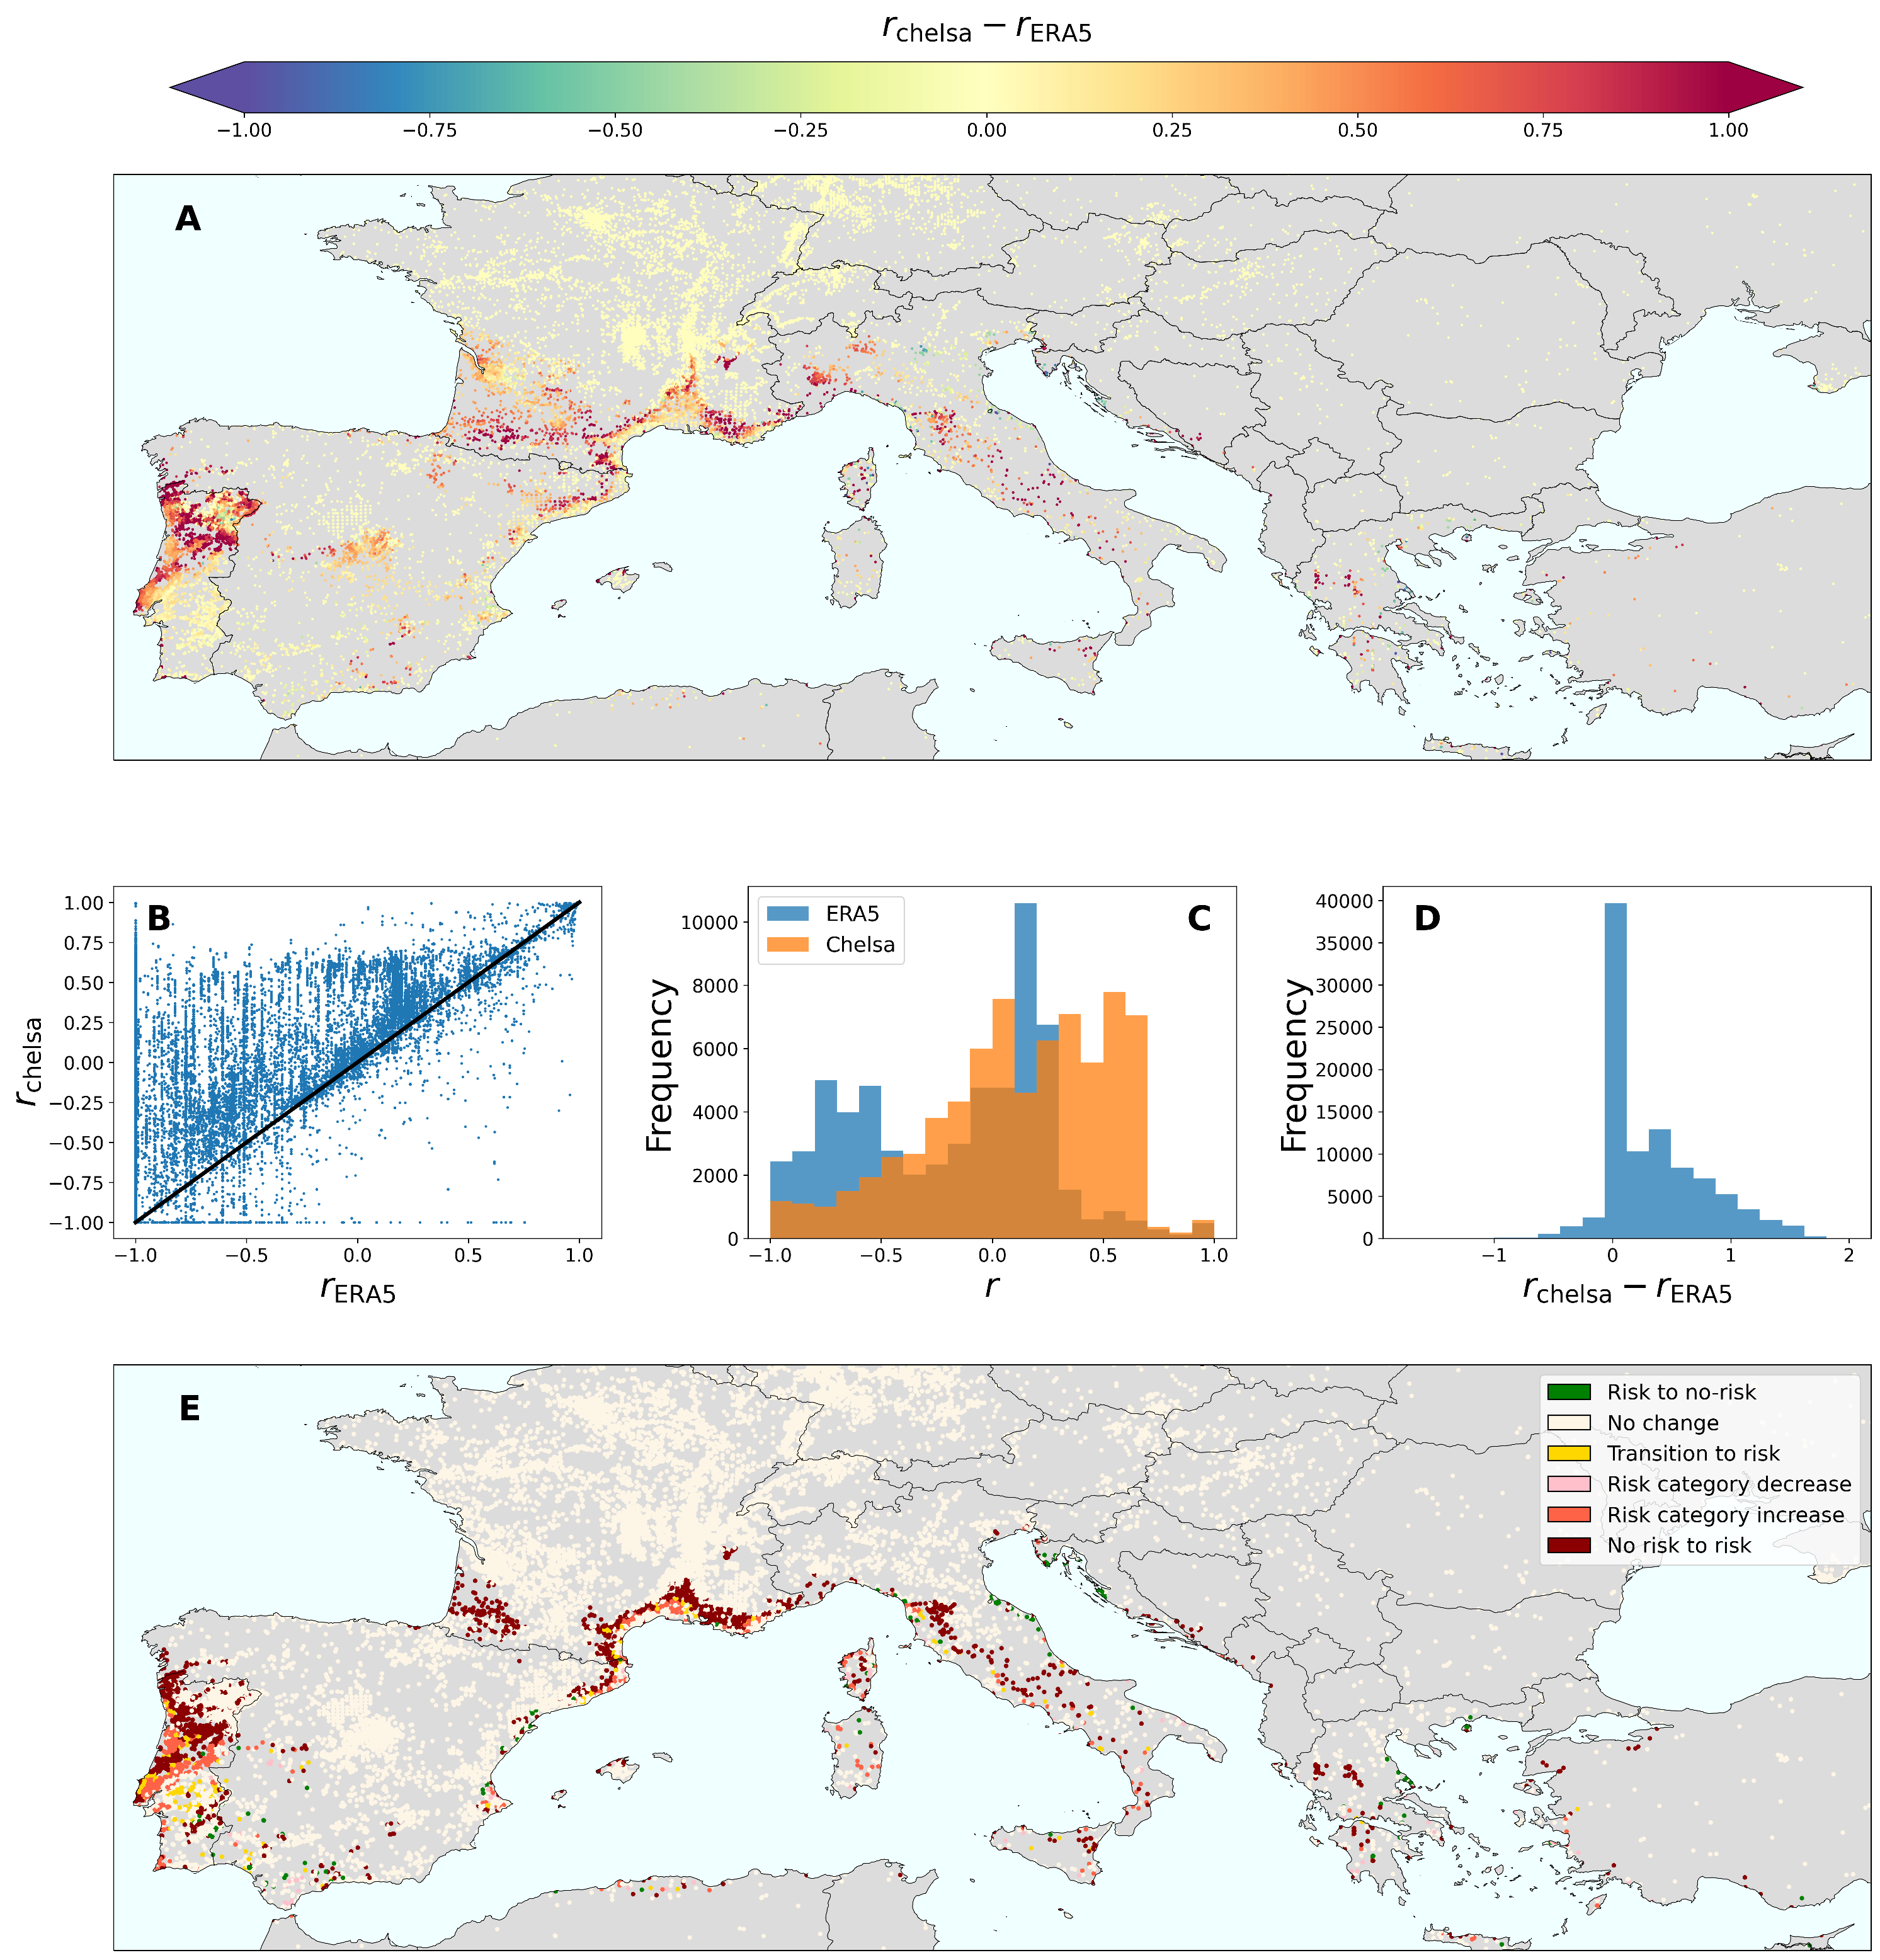
\includegraphics[width=0.9\textwidth]{Figures/risk_difference_vineyards.pdf}
    \caption{Impact of high-resolution climate data on the risk of Pierce's
        Disease for grapevines worldwide. (A) Difference in risk indices in
        Europe,
        which accounts for the 96\% of the points in the dataset. (B)
        Comparison of the
        risk indices derived from CHELSA and ERA5 datasets. Points with perfect
        agreement would lie in the solid black diagonal curve. (C) Histogram of
        risk
        indices derived from ERA5 (blue) and CHELSA (orange). (D) Histogram of
        the
        differences in risk indices between CHELSA and ERA5 datasets. (E)
        Changes in
        risk categories when using high-resolution climate data (CHELSA) with
        respect
        to mid-resolution data (ERA5). Risk category increase refers to changes
        from
        low to moderate risk or from moderate to high risk. Likewise, risk
        category
        decrease refers to changes from moderate to low risk or high to
        moderate risk.}
    \label{fig:risk_dif_vid}
\end{figure}

Finally, to obtain a comprehensive assessment of the impact of
microclimatic conditions on the risk of PD establishment, we collated a dataset
of over 100,000 \textit {Vitis vinifera} presence locations worldwide from GBIF
\cite{GBIF}, with a predominant concentration of points from Europe
(Online Supplementary Information). Each data point was assigned a risk index
based on
the ERA5 and CHELSA projections, respectively, using the nearest pixel from
each database.

This approach revealed an increase in the risk indices
associated with the vine locations (\cref{fig:risk_dif_vid} A-D), mostly
showing shifts towards higher risk indices (\cref{fig:risk_dif_vid} A,E) from
no risk to risk, or increases in risk category (low to moderate or moderate to
high), while a negligible number of points decreased in risk category
(\cref{fig:risk_dif_vid} E). Such behaviour was common to all key viticulture
regions studied, although the extent of increases differed between continents,
with substantial expansion of vineyard areas at risk in Europe and South Africa
(\cref{tab:risk_increase_vid}). Overall, our results emphasise the global
relevance of microclimatic conditions in influencing the risk landscape for PD
in viticultural areas (\cref{tab:risk_increase_vid}).

\begin{table}[H]
    \centering
    \caption{Comparison of grapevine presence locations at risk in key
        viticulture regions using CHELSA and ERA5 datasets}
    \label{tab:risk_increase_vid}
    \resizebox{\textwidth}{!}{%
        \begin{tabular}{lccc}
            \hline \hline
                                   & \multicolumn{1}{l}{\textbf{Nº points}}
                                   & \multicolumn{1}{l}{\textbf{risk
            CHELSA (\%)}}          & \multicolumn{1}{l}{\textbf{risk ERA5
                    (\%)}}
            \\ \hline
            \textbf{Europe}        & 96102
                                   & 41.2                                   &
            21.8
            \\
            \textbf{USA}           & 792
                                   & 69.8                                   &
            66.3
            \\
            \textbf{South Africa}  & 36
                                   & 47.2                                   &
            5.6
            \\
            \textbf{South America} & 112
                                   & 77.7                                   &
            74.1
            \\
            \textbf{Australia}     & 186
                                   & 51.6                                   &
            45.7
            \\ \hline \hline
        \end{tabular}%
    }
\end{table}

\section{Discussion}

Our study sheds light on the  relevance of the spatial scale of observation
in the intricate interplay between microclimatic conditions and the risk of PD
for grapevines on a global scale. The use of high-resolution climate data
reveals previously unrecognised local areas with microclimates conducive to the
establishment of PD worldwide. Contrary to the simplistic assumption that
higher resolution data might yield only marginal distinctions at regional
levels, our study demonstrates that slight variations in climate data at local
scales can lead to a global surge in disease risk. These increases  not only
affect the spatial distribution of risk, but also its temporal dimension, as
suggested by the rate of increase in the surface area at risk. In the case of
PD, we show that this rate nearly doubles when high-resolution climate data is
considered compared to previous estimates obtained with mid-resolution data.
Thus, our findings indicate a critical need for the use of local or
high-resolution climate data in the assessment of disease risk, especially in
areas characterised by diverse topography and even when only attempting to
global estimates.

Such observed differences arise from the non-linear nature of disease
dynamics and the response of the pathosystem components to environmental shifts
\cite{scherm1994global,Dudney2021}. Therefore, models dependent on broader
climate data may not capture the complexities of microclimates, resulting in an
underestimation of disease risk.  While this is not inherently negative,
recognising these limitations helps to assume such risk estimates as a
conservative lower bound until proven otherwise . Acknowledging these
constraints is crucial for refining our understanding of disease dynamics and
ensuring that our risk assessments are sufficiently cautious in the absence of
more reliable data. Likewise, data coarsening procedures should be avoided, if
possible, when modelling climate-driven disease dynamics, even in spite of
computational efficiency. This recommendation applies not only to disease risk
predictions but to all those in which non-linear functions depending on climate
variables are present, such as species distribution models or phenological
models \cite{menzel2006european}.

Despite the valuable insights gained,  our analysis heavily relies on the
quality and resolution of the climate data from the CHELSA dataset
\cite{chelsa-climatologies-2021}. While this dataset offers information at a
high spatial resolution, the temporal dimension is limited to a daily
frequency, which forces to apply an approximation to infer hourly data.
Furthermore, the data may still be subject to biases or uncertainties inherent
to the nature of the methodology employed in their construction . On the other
hand, vector presence data is only accurately obtained for Europe, while an
homogeneous presence is assumed in other viticulture areas. Additionally, the
study primarily focuses on the effect of temperature conditions and the
presence of potential vectors to determine the risk of	Xf establishment, which
may not encompass all possible contributing factors. Other variables, such as
soil characteristics or vineyard management practices were not explicitly
considered in this analysis, leaving room for additional complexities in the
disease dynamics. Furthermore, the study predominantly examines the risk at a
global scale, and the applicability of the findings to specific local contexts
may vary.

Future research should aim to address the aforementioned limitations and
provide a more comprehensive understanding of the multiple interactions
influencing PD development  in viticulture regions. Other factors influencing
disease spread, such as human behaviour, land use changes, and ecological
shifts, should also be explored, offering a more comprehensive and holistic
view of the interplay between environmental conditions and disease
vulnerability. The acceleration in the rate at which the risk of PD is growing
calls for more research into control strategies to mitigate its impact on
grapevine crops worldwide.

Although PD is currently restricted to North America and recently
introduced in Taiwan \cite{su2013pierce}, Mallorca (Balearic Islands, Spain)
\cite{gomila2019draft,moralejo2019insights} and Israel
\cite{zecharia2022xylella}, since the mid-1990s climatic conditions are
increasingly conducive to the establishment of PD in southern Europe
\cite{GimenezRomero2022_CommsBio}. For example, with the increase in the
resolution of
climate data our model predicts  the recent detection of PD in Portugal
\cite{loureiro2023xylella}, which was not anticipated using the ERA5 data
\cite{GimenezRomero2022_CommsBio}. In a short time, it is foreseeable that
there will
be more epidemic outbreaks in vineyards in southern Europe if the entry of
infested plants is not controlled. This not necessarily have to be vines but
can also include other plants such as almond trees or ornamental plants
\cite{moralejo2020phylogenetic}.

Overall, our study contributes to the growing body of knowledge on the
impact of climate on agricultural pests and pathogens, emphasising the
importance of considering microclimatic conditions for a more deep
understanding of disease dynamics. Future research should focus on developing
comprehensive models that integrate high-resolution climate data, considering
both the global and local factors that influence disease dynamics. This
holistic approach will enable a more accurate prediction of disease risk,
allowing for the development of targeted management strategies and the
enhancement of global food security.

\section{Methods}

\subsection{Climate data}

Climate data was downloaded from two datasets for our analysis: the ERA5
dataset \cite{munoz-sabater_era5-land_2021, munoz2019era5land} and the CHELSA
dataset \cite{Karger2017, chelsa-climatologies-2021}. ERA5 offers
mid-resolution climate data with a spatial resolution of 10 km and hourly
temporal resolution, while CHELSA provides high-resolution data with a spatial
resolution of 1 km and daily temporal resolution. Both datasets exhibit global
coverage and encompass crucial climate variables, such as temperature and
precipitation. For our simulations, we used the mean hourly temperature data
from ERA5 dataset and the maximum and minimum daily temperature data from
CHELSA dataset.

\subsection{Vector climatic suitability}

Vector climatic suitability data was obtained from \cite{Godefroid2022}, in
which a Generalised Additive Model (GAM) is employed to calibrate the
relationship of \textit{P. spumarius} global occurrence with moisture index and
maximum temperatures during summer index estimated from 1979 to 2013 using the
CHELSA dataset.

\subsection{Vineyard data}

To assess the risk of Pierce's Disease in locations where grapevines are
present, we collected a comprehensive dataset of over 100,000 \textit{Vitis
    vinifera} presence data records from the Global Biodiversity Information
Facility (GBIF) \cite{noauthor_what_nodate,GBIF}. We note that while the
dataset spans the globe, 96\% of the points are located in Europe
(Online Supplementary Information).

\subsection{Climate-driven epidemiological model}

We used the model developed in \cite{GimenezRomero2022_CommsBio}, which
describes
the initial exponential rise (or decrease) of infected plants at the onset of
an epidemic based on the spatial distribution of the vector and the bacterial
growth and survival processes mediated by temperature. The density of vectors
at a given cell controls the number of new plants that will be inoculated with
the bacterium, while the local temperature mediates the growth and survival
processes of the in-plant bacterial population, leading the initial inoculation
to an infection or not. These temperature-driven growth and survival processes
are described with the accumulation of two metrics denoted \textit{Modified
    Growing Degree Days} (MGDD) and \textit{Cold Degree Days} (CDD). The base
function to compute the MGDD is proportional to the Xf temperature-dependent
growth rate and is defined by
\begin{align*}
     & f(T)=\left\{\begin{array}{lll}
                       0                & \textrm{if} & T<T_{\textrm{base}}
                       \\
                       m_1\cdot T-b_1   & \textrm{if} & T_{\textrm{base}} \leq
                       T < T_1
                       \\
                       m_2\cdot T + b_2 & \textrm{if} & T_{1} \leq T <
                       T_{\textrm{opt}}
                       \\
                       m_3 + b_3        & \textrm{if} & T_{\textrm{opt}} \leq T
                       < T_2
                       \\
                       m_4 + b_4        & \textrm{if} & T_2 \leq
                       T_{\textrm{max}}
                       \\
                       0                & \textrm{if} & T\geq T_{\textrm{max}}
                   \end{array}\right. \,
\end{align*}
where $T_{\textrm{base}}=\SI{12}{\degree C}$, $T_1=18$,
$T_{\textrm{opt}}=\SI{28}{\degree C}$,	$T_2=32$ and
$T_{\textrm{max}}=\SI{35}{\degree C}$; the slopes are $m_1= 0.66$, $m_2=1$,
$m_3=-1.25$ and $m_4=-3$ and the intercepts are $b_1=-8$, $b_2=-14$, $b_3=4$
and $b_4=105$. MGDD are then computed as
\begin{equation}\label{eq:MGDDdef}
    MGDD(t) = \frac{1}{24}\sum_{\tau \in t} f(T(\tau)),
\end{equation}
where $\tau$ is expressed in hours, $t$ in years and we divide by $24$ to
obtain $MGDD(t)$ in degree days. The accumulation period goes from the
$1^{\mathrm{st}}$ of April to the $31^{\mathrm{st}}$ of October in the northern
hemisphere and from the $1^{\mathrm{st}}$ of November to the $31^{\mathrm{st}}$
of March in the southern hemisphere.

CDD are computed between $1^{\mathrm{st}}$ November and $31^{\mathrm{st}}$
March in the northern hemisphere and between $1^{\mathrm{st}}$ April and
$31^{\mathrm{st}}$ October in the southern hemisphere as
\begin{equation}
    CDD(t)= \frac{1}{24}\sum_{\tau \in t} (6-T(\tau)) \ \quad \textrm{for}
    \quad T_i\le 6\textrm{\textdegree C} .	\label{eq:CDDdef}
\end{equation}

Altogether, the number of infected hosts is described by the following
recurrence relation
\begin{equation}
    I(t)=I(t-1)e^{\gamma(R_0-1)}\mathcal{F}(MGDD(t))\mathcal{G}(CDD(t)) \ ,
\end{equation}
where $\gamma$ is the death rate of infected vines, $R_0$ is the basic
reproduction number of the disease and $\mathcal{F}(\cdot)$ and
$\mathcal{G}(\cdot)$ are sigmoidal-like functions that relate the MGDD and CDD
metrics to the probability of developing an infection from a given inoculation.
Following \cite{GimenezRomero2022_CommsBio}, $R_0$ in each cell $j$ is related
to the
climatic suitability of the vector such that
\begin{equation}
    R_0^j=R_0^*\cdot s_j=5\cdot s_j \ ,
\end{equation}
$\gamma=0.2$ and the specific form of $\mathcal{F}(\cdot)$ and
$\mathcal{G}(\cdot)$ is given by
\begin{align}
    \mathcal{F}(x) & = \frac{1}{1+e^{-0.012(x-975)}}        \\
    \mathcal{G}(x) & = \frac{2\cdot10^7}{2\cdot 10^7 + x^3}
\end{align}

Finally, the risk index is derived as the effective growth rate of the
infected population over the simulated time \cite{GimenezRomero2022_CommsBio},
\begin{equation}
    r_j=\max\left\{-1, \frac{\ln(I_j(T) / I(0))}{\gamma(R_0^j-1)\cdot
        T}\right\} \ .
\end{equation}

Because the typical time scale of the disease is 5 years ($1/\gamma$)
\cite{Almeida2003}, we simulate periods of 7 years. If more years are available
to simulate, we perform a re-introduction of the disease as a single infected
plant in each cell after each 7-year period
\cite{GimenezRomero2022_CommsBio}.

The code used to run the model is freely accessible at GitHub
\cite{CODE_model}.

\subsection{Model adaptation to daily temperature data}

MGDD and CDD metrics were originally defined using hourly temperature data
(\cref{eq:MGDDdef,eq:CDDdef}) \cite{GimenezRomero2022_CommsBio}. However, the
CHELSA
dataset only provide daily granularity. To overcome this limitation, we use a
basic sinusoidal extrapolation relating maximum and minimum daily temperature
to hourly temperatures,
\begin{equation}
    T_h=\frac{T_{max}+T_{min}}{2} + \frac{T_{max}-T_{min}}{2}\sin(w\cdot h)
    \ ,
\end{equation}
with $w=2\pi/24$ and $h$ ranging from $0$ to $23$. This approximation was
validated in \cite{GimenezRomero2023_PD} with data from national meteorological
stations
in Spain (AEMET) using several locations and years, showing no differences
between the use of hourly or daily temperatures to estimate MGDD and CDD.
Similarly, the use of the approximation was validated across Europe using
EURO-CORDEX data.


%----------------------------------------------------------------------------------------
%	PART IV: Data-driven methods for global ecological problems
%----------------------------------------------------------------------------------------
{
	\hypersetup{hidelinks}
	\part{Data-driven methods for global ecological problems}
}
\thispagestyle{empty}

\begin{center}
    \textbf{\Large Summary}
\end{center}

In an era where ecological issues are becoming increasingly complex and
globalized, the integration of data-driven methodologies into ecological
research offers unprecedented opportunities for addressing these challenges.
The last part of this thesis explores the application of such methodologies to
study global ecological problems related to coastal marine ecosystems: the
decline of coral reefs, the acidification of coastal waters, and the loss of
seagrass meadows. Coral reefs are among the most biodiverse ecosystems on
Earth, providing essential services to marine life and coastal communities.
However, they are threatened by a combination of human activities and climate
change, which have led to widespread coral bleaching events and the loss of
coral cover. The acidification of coastal waters is another pressing issue
posing significant risks to marine life, particularly species that rely on
calcium carbonate for their skeletal structures like coral reefs. Seagrass
meadows are also under threat from human activities, such as coastal
development and pollution, which have led to the loss of seagrass habitats and
the decline of associated biodiversity. The understanding of the spatiotemporal
dynamics of these ecosystems together with the monitoring of their health and
factors affecting their resilience is crucial for effective conservation and
management strategies. However, this is often challenging due to the complexity
of these ecosystems and the difficulty of collecting data at the necessary
spatial and temporal scales. By leveraging large existing datasets, machine
learning algorithms, and spatial analysis, here we provide novel insights
into the spatial properties of coral reefs, the reconstruction of pH
time-series in coastal waters, and the mapping of seagrass meadows from
satellite imagery. These case studies exemplify the potential of data-driven
approaches to enhance our understanding of ecological dynamics, improve
environmental monitoring, and inform conservation strategies.

\vspace{1cm}

\begin{objectiveslist}
    \item To investigate the spatial properties of coral reefs at a global
    scale.
    \item To reconstruct pH time-series in coastal waters that present missing
    data due to sensor failures.
    \item To map seagrass meadows from satellite imagery.
\end{objectiveslist}

\vspace{1cm}

\begin{contributionslist}
    \item We obtained universal scaling laws that describe the spatial
    properties of coral reefs at a global scale.
    \item We describe 4 macroecological patterns that emerge from the spatial
    properties of coral reefs: the size-frequency distribution, the
    perimeter-area relationship, the inter-reef distance distribution and
    the
    reefscape fractal dimensions.
    \item We developed a novel method to reconstruct pH time-series in coastal
    waters from parallel measurements of temperature, salinity and
    dissolved
    oxygen.
    \item We developed a deep learning model to map seagrass meadows from
    satellite imagery, which outperforms traditional methods.-
\end{contributionslist}

%----------------------------------------------------------------------------------------
%	Universal spatial properties of coral reefs	
%----------------------------------------------------------------------------------------
\chapterimage{coral_reefs.jpg}
\chapterspaceabove{6.75cm}
\chapterspacebelow{7.25cm}

\chapter{Universal spatial properties of coral reefs}
\vspace{1cm}

\begin{center}
    \textbf{Àlex Giménez-Romero$^{1}$, Manuel A. Matías$^{1}$, Carlos M.
        Duarte$^{2}$}
\end{center}

\vspace{1cm}

\begin{enumerate}
    \small
    \item Instituto de Física Interdisciplinar y Sistemas Complejos, IFISC
          (CSIC-UIB), Palma de Mallorca 07122, Spain
    \item Tragsa, Passatge Cala Figuera 6, 07009 Palma de Mallorca, Spain
\end{enumerate}

\vspace{1cm}

\textbf{Published as}

\vspace{0.5cm}

%\fullcite{GimenezRomero2024}

\newpage
\section{Introduction}

Coral reefs form some of the largest biogenic structures in the biosphere
\cite{wiener2021exploration}, and are prevalent structures across tropical
coastal waters. Coral reefs often form complex, labyrinthine structures that
render sailing in tropical waters challenging, but protect the shorelines of
tropical coastal nations while supporting biodiversity and providing food
supply supporting local communities \cite{Moberg1999}. The formation of coral
reefs has intrigued scientists for a long time, with Darwin formulating a model
based on coral reefs accreting on volcanic structures
\cite{darwin1874structure}. Darwin's model continues to stir discussion
\cite{Droxler2021}, as it would represent a class of coral reefs, at best,
among the broad range of configurations and possible origins
\cite{Scoffin1983}.

Coral reefs can form isolated oval or ring-shaped structures (e.g. coral
atolls), linear structures parallel to the shoreline (fringing or barrier
reefs) or convoluted or highly-branched structures (e.g. \cite{Purkis2007}),
and often present nested structures, such as smaller reefs within large coral
reef lagoons \cite{Bradbury1983}. Whereas previous studies have examined the
geometry of coral reefs \cite{Bradbury1983,Purkis2007,
    Zawada2009,Alvarez_Filip2009,Bozec2015, Sous2020}, finding evidences of
fractality both at individual reef \cite{Bradbury1983,Sous2020} or regional
scales \cite{Purkis2007, Zawada2009}, a global assessment of coral reef size
and geometry was hitherto precluded by the lack of data on reef form and size
at the global scale. Resolving the size and geometry of coral reefs has become,
however, a matter of urgency, as coral reefs are rapidly declining, with an
estimated 50\% of coral cover lost globally from 1957-2007
\cite{eddy2021global}. The IPCC projects that 70\% to 99\% of coral cover may
be lost if climate change reaches 1.5 to 2.0 ºC above pre-industrial levels,
respectively \cite{bindoff2019changing}. Yet, the Kunming-Montreal Biodiversity
Framework \cite{kunming-montreal-framework} calls for stopping all biodiversity
losses and restore 30\% of degraded habitats, including coral reefs, by 2030,
which requires action at individual reefs and, therefore, an understanding of
coral reef form and size as an underpinning for the necessary conservation
action.

The release of the Allen Coral Atlas (ACA) \cite{allen-coral-atlas}, a
worldwide mapping initiative that provides benthic habitat data of
shallow-water (above 10 m deep) tropical reefs, presents an unprecedented
opportunity to characterize the form and size of coral reefs on a global scale.
In contrast to previous efforts, such as NOAA’s Coral Reef Information System
\cite{oconnor2020}, Khaled bin Sultan Living Oceans Foundation
\cite{globalreefexpedition2021} or Millennium Coral Reefs \cite{unep2010}, the
ACA dataset combines an extensive global coverage of reef areas with the direct
availability of processed habitat data obtained from recent high-resolution
(3\,m) satellite imagery using deep learning models. This invaluable resource
offers a unique vantage point for researchers, scientists, and conservationists
to explore and understand coral reef ecosystems in ways that were previously
challenging or impossible. This requires processing the classified images to
extract a canonical inventory of individual coral reefs that can be used to
derive macroecological laws and principles from the patterns and trends
observed across coral reefs. This, in turn, enables to advance and consolidate
our understanding of these complex ecosystems and the scale of the effort
required to conserve and restore them.

Here we report universal macroecological patterns
\cite{Brown1995Macroecology} in shallow-water, tropical coral reef size and
geometry using data from the 2022 release of the ACA \cite{allen-coral-atlas}.
Specifically, we produced a global inventory of individual reefs
\cite{gimenez_romero_2023_10025083}, allowing the analysis of the size and
inter-reef distance distributions of individual coral reef areas within each
coral province of the Atlas. We then examined the relationship between reef
size, shape and fractal geometry of coral reefs.

\section{Results}
\subsection{Coral reefs macroecological patterns}

The area of all coral reefs within each province of the ACA was computed
after processing the data to identify individual reefs (see Methods). We
identified a total of $1,579,772$ individual shallow-water tropical reefs,
extending over a total of $52,423$ $km^2$ of ocean area. The canonical nature
of this openly available dataset (see Methods), which includes all
shallow-water tropical coral reefs worldwide, allows the mean and median size
of individual reefs to be estimated at \SI{3.32}{ha} and \SI{0.3}{ha},
respectively, across all coral reef provinces in the Atlas (see
\cref{tab:Province statistics} for statistics in each province).

Our analysis reveals that the size distribution of the area of coral reefs
in all provinces converge to conform a power-law distribution, $y\sim
    x^{-\alpha}$, that holds over multiple scales, where $y$ reflects the
probability of ocurrence of reefs of area class $x \ km^2$
(\cref{fig:general_analysis} a-b). This behavior was consistent across all
provinces within a range of 3 to 5 decades in coral reef area, yielding an
average exponent of $\left<\alpha\right>=1.84$ ($95\%$ CI: $1.55$ to $2.12$)
(see Methods). The global size-frequency distribution of coral reefs, fitted to
all data independently on the province, conforms to a power-law with an
exponent of $\alpha=1.8$, consistent with the mean exponent
$\left<\alpha\right>$, providing evidence for a universal scaling law governing
the size distribution of coral reefs. This suggests that the observed
distribution of reef areas arises mainly due to biological processes
contributing to reef formation, common among the provinces. Local geophysical
processes interacting with coral reef growth, which might vary among provinces,
are therefore likely to have a limited role, provided the universality of the
power-law scaling of the reef size distribution.

\begin{figure}[H]
    \centering
    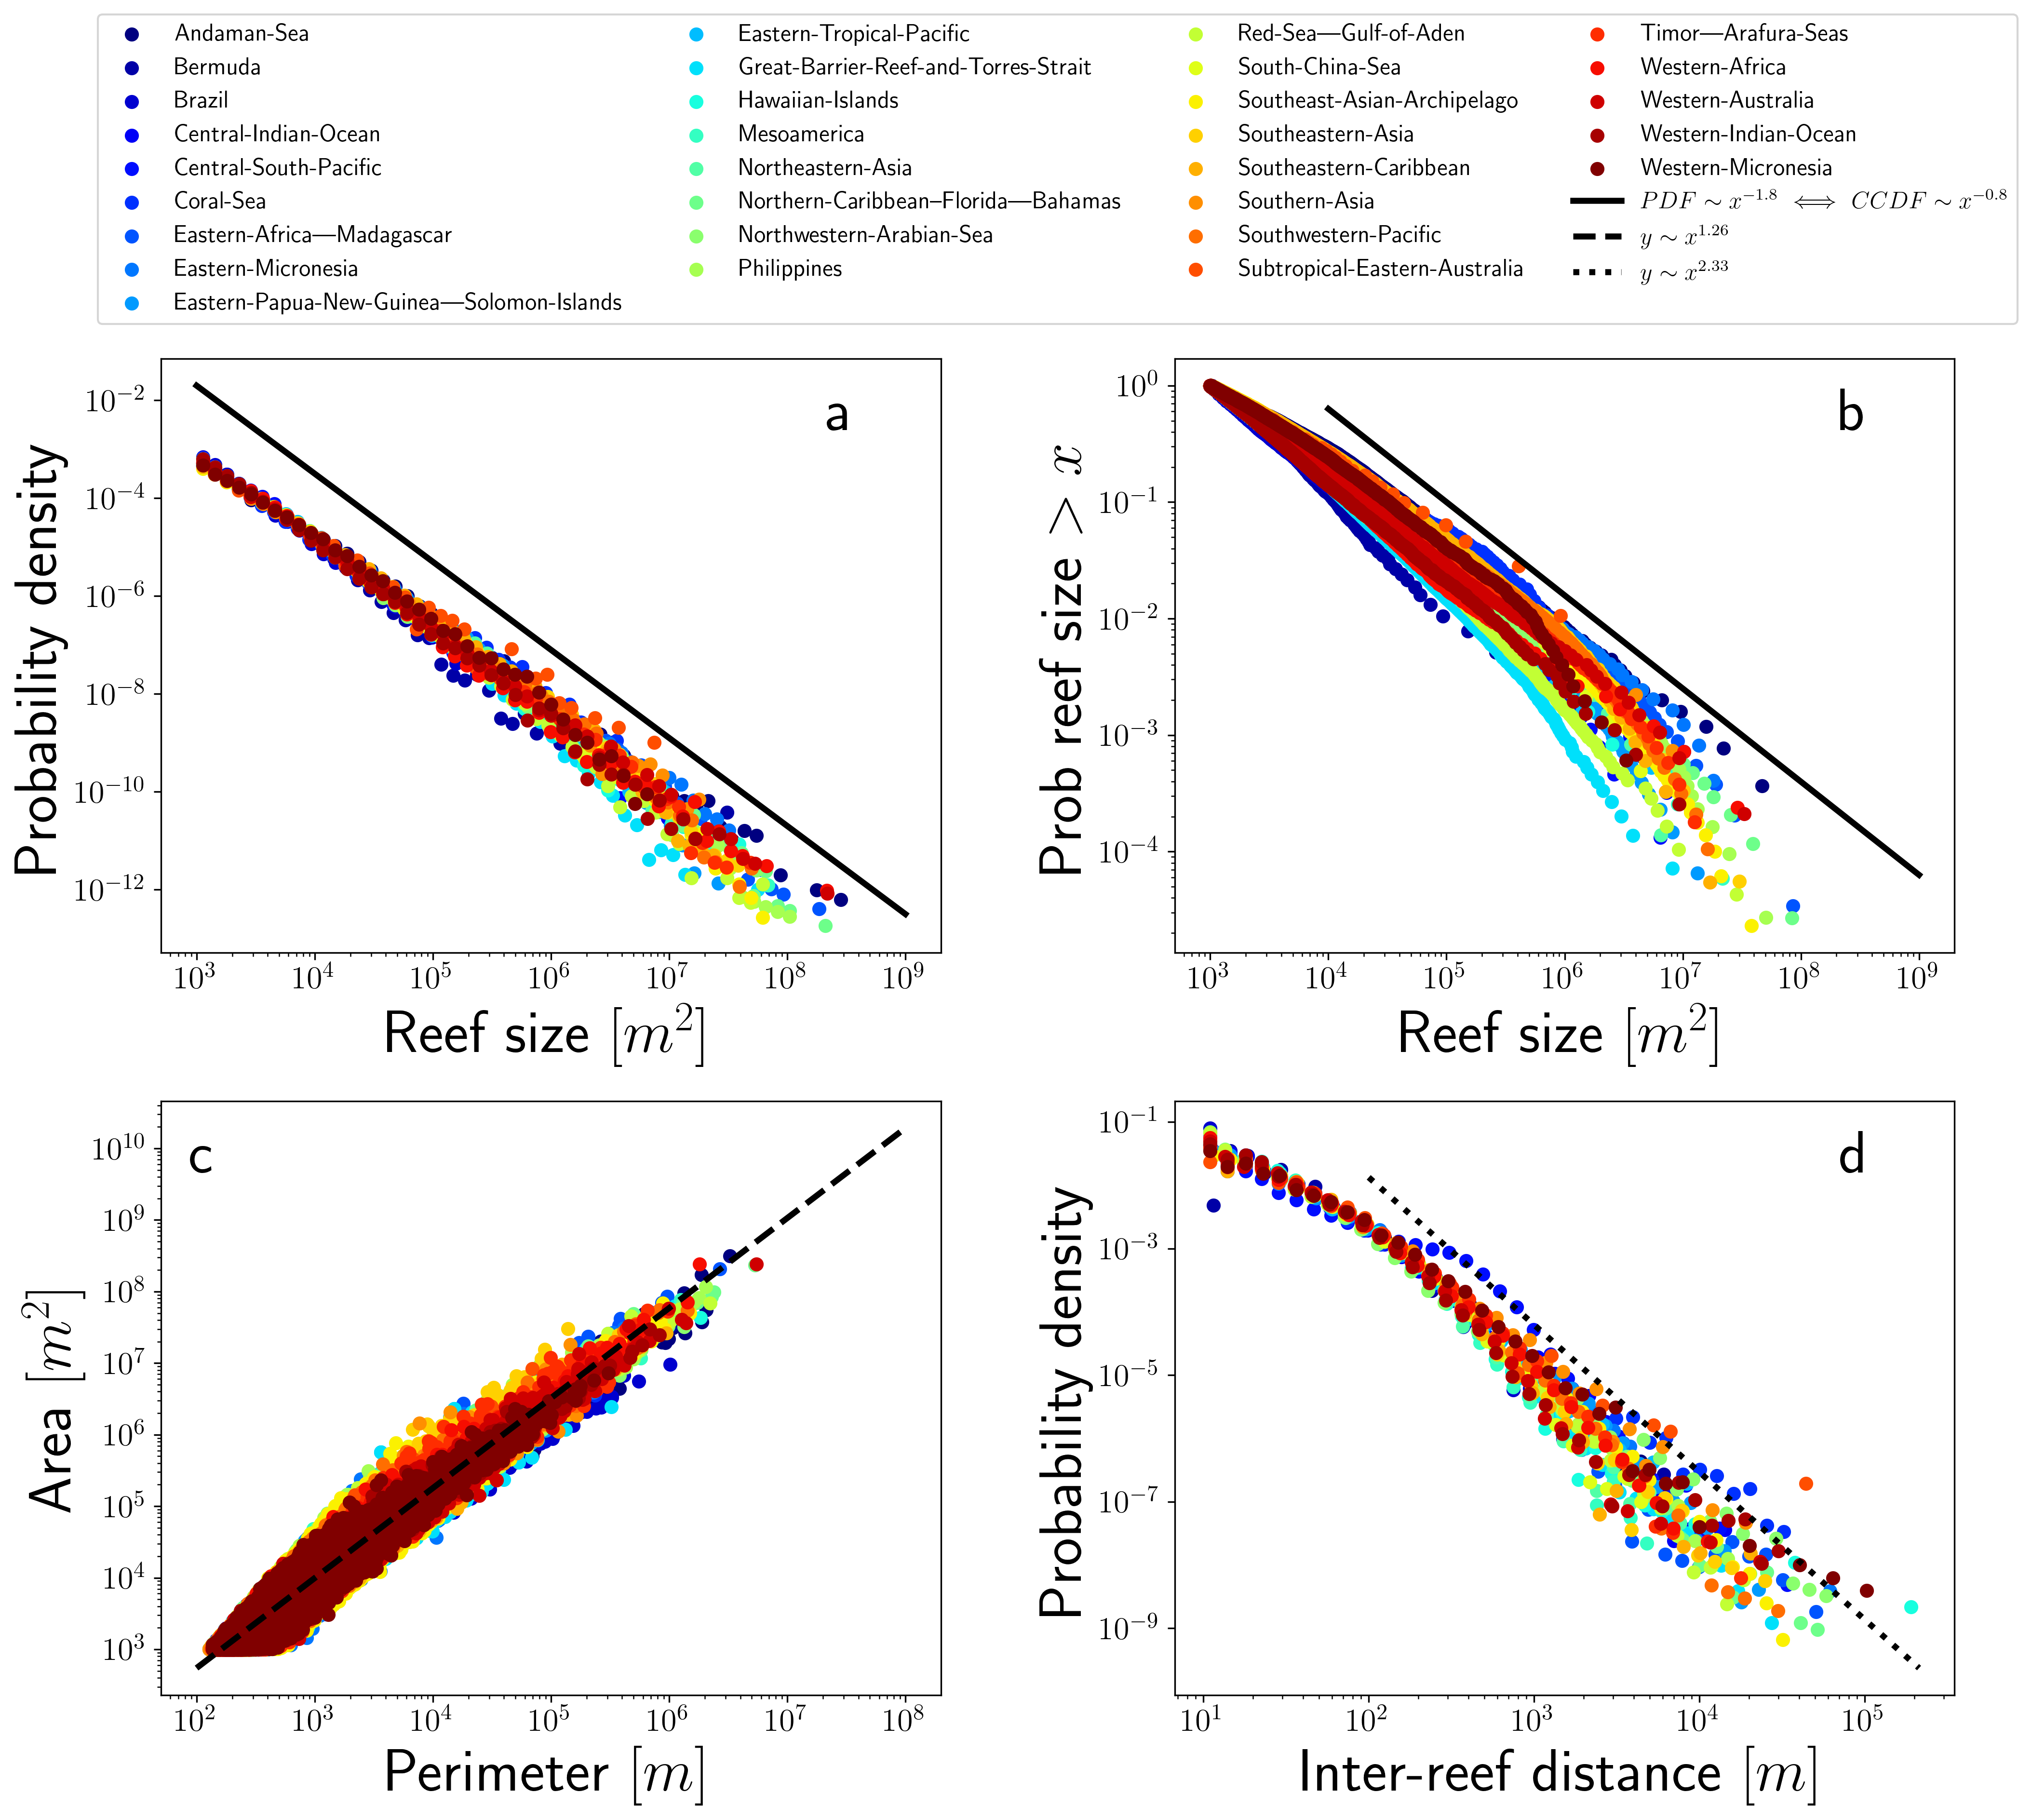
\includegraphics[width=\textwidth]{Figures/general_analysis.png}
    \caption{\textbf{Macroecological patterns of global coral reef size,
            geometry and spacing.} (a) Size distribution. The black line
        corresponds to a
        fitted power-law of exponent $1.8$. (b) Complementary cumulative
        distribution
        function (CCDF) with corresponding exponent of $1.8$. (c)
        Area-Perimeter
        relation. The black dashed line corresponds to a fitted power-law with
        exponent
        $1.23$. (d) Inter-reef distance distribution. The black dotted line
        corresponds
        to a fitted power-law to the distribution tail with a exponent of
        $2.33$.}
    \label{fig:general_analysis}
\end{figure}

The presence of a power-law size distribution also suggests that the object
studied may be fractal in nature \cite{Mori2020, PINTO2014, Seekell2013,
    Sorensen1999, Vidondo1997}, at least along a certain range. A simple way to
test whether coral reefs are fractals is using the area-perimeter relation
\cite{MAN83, Lovejoy1982}, a method of fractal analysis that characterizes the
complexity of irregular shapes by examining the relationship between their area
and perimeter (see Methods). The scaling of coral reef area to perimeter of all
individual coral reefs also converges into a single power-law with an exponent
of $\alpha=1.2578$ ($95\%$ CI: $1.2573$ to $1.2583$), indicating again a
universal behavior (\cref{fig:general_analysis} c). When the relationship is
fitted for each province independently, we found a mean exponent of
$\left<\alpha\right>=1.2574$ ($95\%$ CI: $1.1757$ to $1.3391$), practically
identical to the general exponent. The exponent for the area-perimeter
relationship is significantly lower than the value of $2$ that would be found
for a smooth euclidean geometry. According to fractal analysis, the fractal
dimensions of the perimeter and area of coral reefs are given by $D_P=1.2950$
and $D_A=1.6289$ (see Methods), respectively, which are clearly different than
the putative euclidean dimensions of $D_P=1$ and $D_A=2$. Taking each province
independently, these fractal dimensions would vary between
$D_P^{\mathrm{max}}=1.3506$, $D_P^{\mathrm{min}}=1.2468$ and
$D_A^{\mathrm{max}}=1.6696$ and $D_A^{\mathrm{min}}=1.5879$ within a 95\%
confidence interval, further ensuring that the obtained fractal dimensions are
significantly different from the euclidean geometry. Coral reefs develop
fractal-like geometries, exhibiting complex, self-similar structures across
different scales. This feature might arise from the complex physical and
ecological processes that shape the distribution and growth of coral reefs.
However, how this occurs remains largely unknown, as we lack mechanistic models
able to generate coral reef landscapes across scales and time that can be
challenged to reproduce these patterns.

The spatial distribution of coral reefs within each province was also
investigated by means of the inter-reef distance, defined as the minimum
distance between a reef and its nearest neighbor. We find a heavy-tailed
relation where the tail conforms to a power-law with an exponent of $2.33$
(\cref{fig:general_analysis} d). This reveals that most of the reefs are close
to each other, while a non-negligible number of them are isolated. This finding
is again mostly independent on the geographic location of the analyzed coral
reefs, arising as a universal property of coral reef provinces.

\subsection{The fractal nature of coral reefs}

We computed the fractal dimension of the area and perimeter of each
individual reef from all provinces using the well-known box-counting algorithm
(see Methods). The mean values for the fractal dimension of the perimeter,
$D_P=1.24$ (95\% CI: 1.13 to 1.35) and the fractal dimension of the area,
$D_A=1.60$ (95\% CI: 1.39 to 1.81), are well defined and consistent with those
obtained from the area-perimeter relationship
(\cref{fig:individual_reef_analysis} a,b). The fractal dimension for the reef
areas is quite stable around the mean, although it increases slightly for large
coral reefs (\cref{fig:individual_reef_analysis} a). On the other hand, the
fractal dimension for the perimeter shows a more pronounced increase as
function of reef size. This indicates that as coral reefs grow, their contour
gets more and more convoluted, increasing its complexity, while its surface
remains geometrically more stable.

To further understand the reef formation process from a geometric
perspective, we computed other shape measurements such as compactness and
elongation indices (see Methods). We observe that the compactness of coral
reefs decreases rapidly with increasing size
(\cref{fig:individual_reef_analysis} c). Two changes of shape are consistent
with this result: transitioning from round to elongated shapes or keeping the
rounded shape while developing holes, reef lagoons, within their surface. These
two processes are not necessarily mutually exclusive, as elongated shapes could
appear from evolution of empty rounded shapes. The results obtained for the
elongation index measurement show that both processes must occur, as reefs
elongation increase with size while showing very high variance. This hypothesis
can be contrasted by examining the different shapes that coral reefs have
formed (\cref{fig:individual_reef_analysis} e).

Altogether, our analysis indicate that coral reefs evolve from simple
rounded filled shapes (high compactness and low elongation index) to more
complex elongated and less compact forms (low compactness and high elongation
index), giving rise to fractal objects with stable surface fractal dimension
and increasing perimeter fractal dimension as they grow
(\cref{fig:individual_reef_analysis} e).

\subsection{Fractality extends up to coral provinces}

The fractal dimension of coral reefs varies across a range of spatial
scales, spanning from individual colonies to entire reef systems
\cite{George2021}. This variability arises from the different physical,
biological, and ecological processes that come into play during the development
of the different structures present at each organization level. The different
coral provinces can be understood as the largest organizational level of these
organisms, and the processes involved in maintaining such big structures should
be different from that of individual reefs, giving rise to a different fractal
dimension.

\begin{figure}[H]
    \centering

    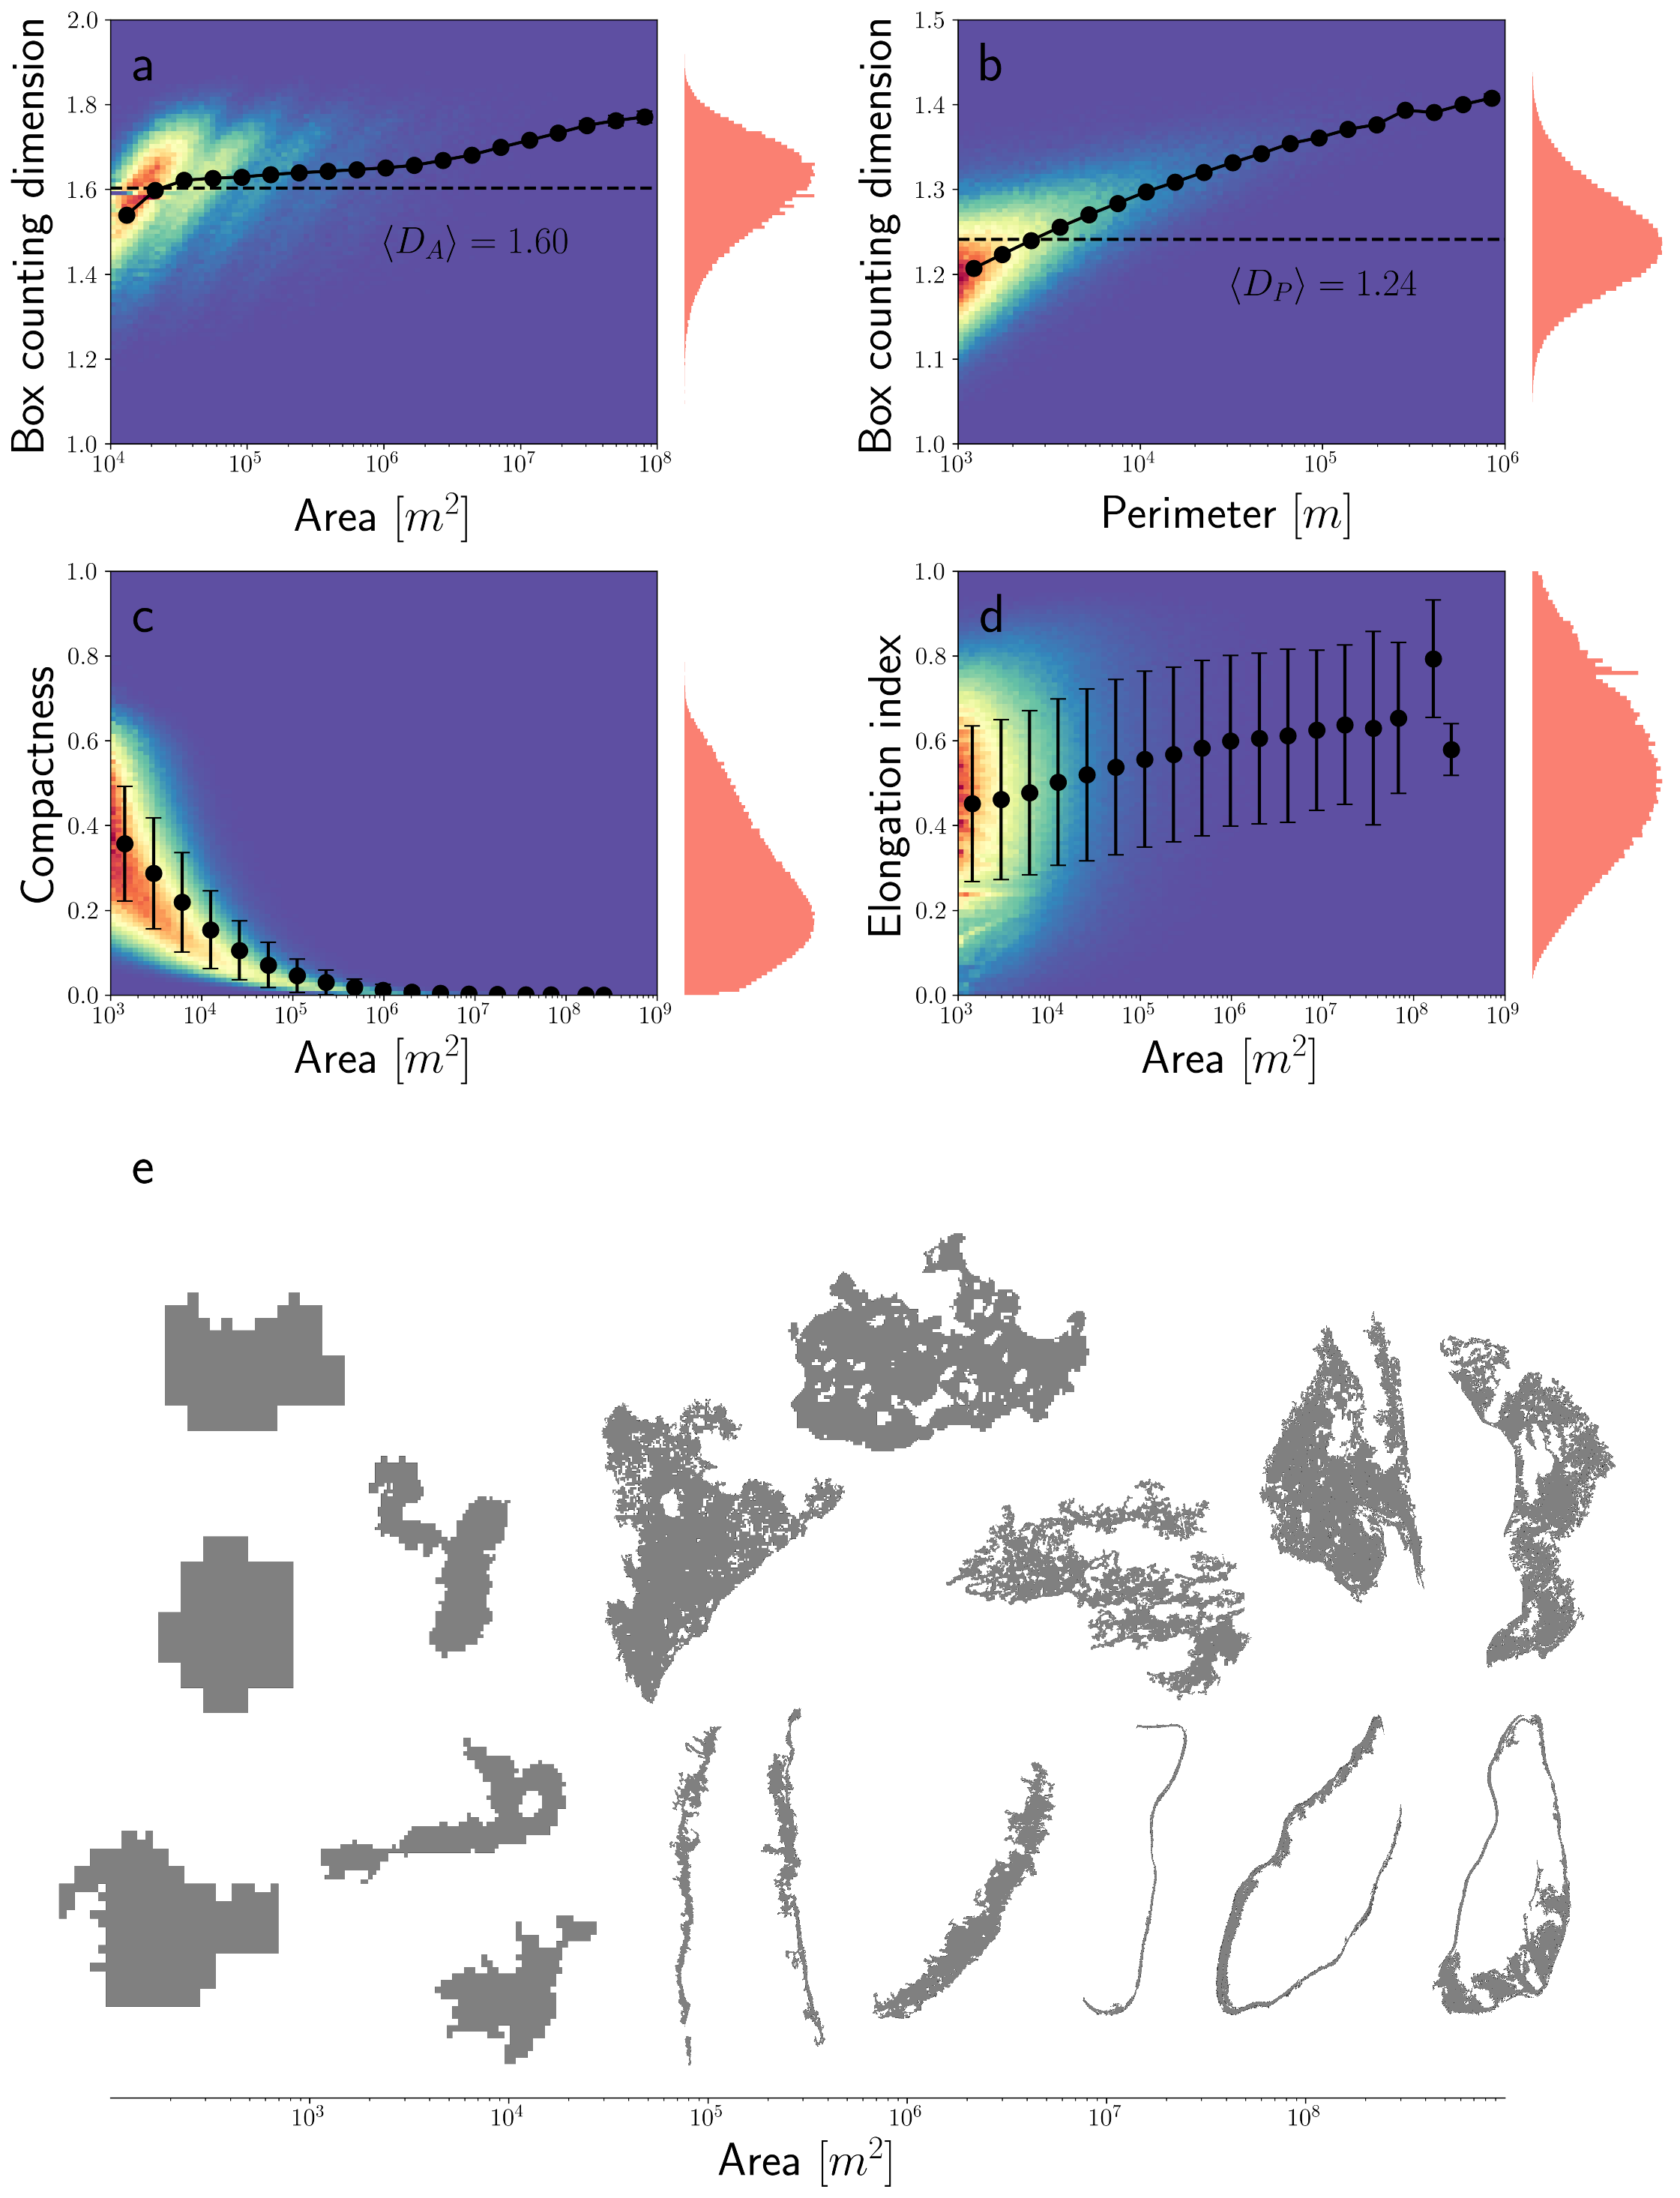
\includegraphics[width=1\textwidth]{Figures/individual_reef_analysis_complete.pdf}
    \caption{\textbf{The fractal nature of global coral reefs.} 2D
        histograms from all shallow-water coral reefs worldwide for: (a) the
        surface
        fractal dimension and area; (b) the perimeter fractal dimension and
        perimeter;
        (c) the compactness and area and (d) the elongation index and area. The
        black
        line corresponds to the mean values of the Y axis measure as function
        of the X
        axis measure. The red histogram corresponds to the distribution of the
        Y axis
        measure. (e) Example of coral reefs shape as function of their
        surface.}
    \label{fig:individual_reef_analysis}
\end{figure}

\begin{figure}[H]
    \centering

    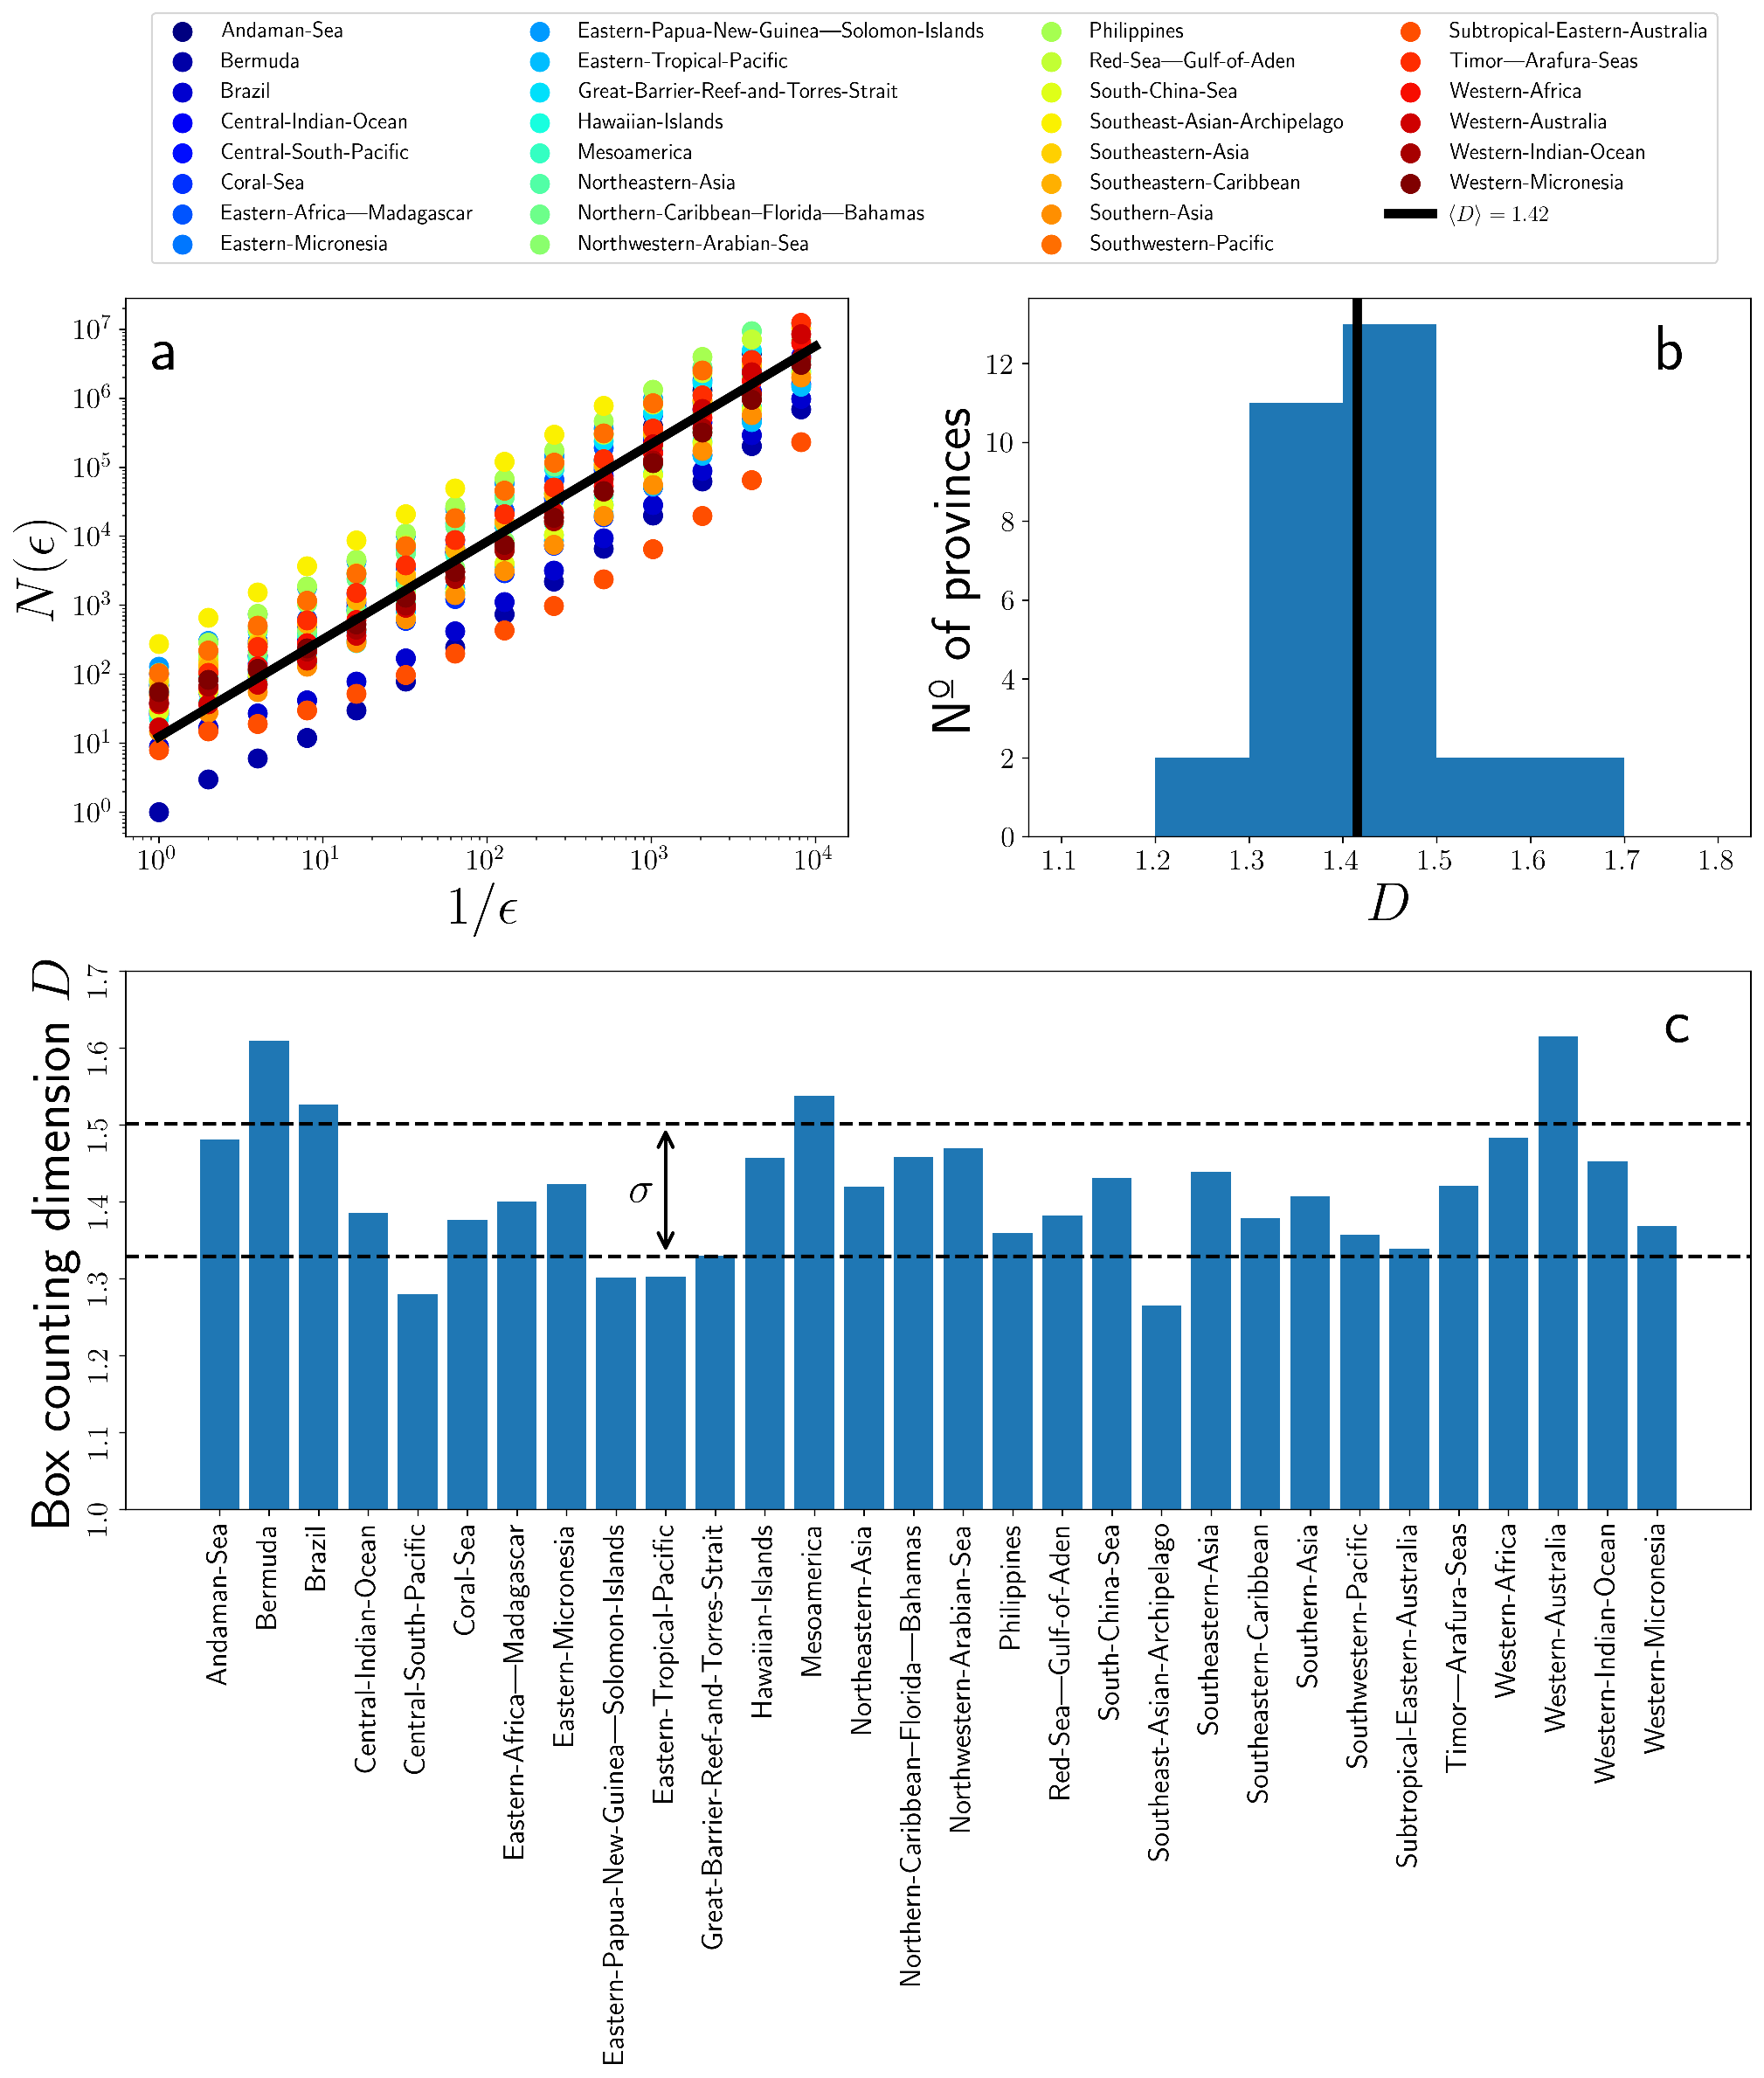
\includegraphics[width=1\textwidth]{Figures/Box_Counting_Dimensions.pdf}
    \caption{Box Counting Dimension of coral reef provinces surface. (a)
        Scaling of the measure (number of boxes of length $\epsilon$,
        $N(\epsilon)$) as
        function of the ruler used (box length $\epsilon$). The slope of the
        fit for
        each province corresponds to its Box-Counting surface fractal
        dimension, $D$.
        (b) Histogram of the obtained Box-Counting fractal dimensions. The
        solid black
        line represents the mean Box-Counting fractal dimension,
        $\left<D\right>$. (c)
        Box-counting surface dimension for each coral province. Black dashed
        lines
        correspond to a 1 $\sigma$ deviation from the mean.}
    \label{fig:Box_Counting_Dimension}
\end{figure}

To investigate this hypothesis, we computed the surface fractal dimension
for each coral province as a whole using the well-known box-counting algorithm
(Methods, \cref{fig:Box_Counting_SI}). We found a mean fractal dimension
of
$\left<D\right>=1.42$ (95\% CI: 1.24 to 1.59), consistent across the different
coral provinces assuming a normal distribution
(\cref{fig:Box_Counting_Dimension}). The fractal dimension of coral reef
landscapes is similar to those expected from sizes expanding along a Fibonacci
series, which yield a fractal dimension of 1.44 \cite{Sorensen1998}. This
suggests, again, that coral reefs are self-organized systems that exhibit
similar patterns of complexity and irregularity at different scales, and that
the fractality is an intrinsic property of coral reefs that likely arise from
the underlying biological, physical, and ecological processes involved in their
growth dynamics.

\section{Discussion}

Coral reefs self-organize to form macroecological patterns that are largely
independent of the geographical location of the reefs, suggesting that the
specific physical conditions to which each coral province is subject have
little influence on the development of these scaling laws. Coral reef
geometries conform fractal structures that follow a power-law size
distribution, with many reefs close to each other while others are completely
isolated across coral reef provinces. Overall, our findings provide strong
evidence that the power-law size distribution of coral reefs and their fractal
geometries are fundamental features of these ecosystems, which reflect the
underlying ecological and physical processes that shape them across scales.
Furthermore, because the exponent of the power-law size distribution and the
fractal dimensions are consistent across different regions, these features are
not only fundamental, but universal laws reflecting coral reef growth
processes.

These universal scaling properties must be used to challenge mechanistic
models aimed at reflecting coral reef growth, which hitherto lacked such
constraints, both as individual reefs as well as coral reef provinces. For
example, at the scale of coral reef province, the characteristic spacing
(inter-reef distance distribution) likely influences the interaction between
coral reefs, hydrodynamic flows, and the dynamics of the limiting nutrients
transported to support photosynthesis and calcification, further constrained by
sea level change and available vertical accommodation space \cite{Nakamura2007,
    Mistr2003, Bosscher1992}. Realistic models of coral reef growth and
dynamics
should be able to reproduce the universal features described here, such as the
power law in coral reef size distribution, the fractal geometries and the
changes in reef shape with size.

Power-law distributions have been also found in many natural systems
\cite{SOLE1995, west2000scaling, Brown2002, Chave2003, Marquet2005,
    Corral2019}.
Different mechanisms can produce such emergent power-laws
\cite{Markovic2014}: Self-Organized Criticality, in which the system evolves
naturally towards a critical state \cite{Per1988}; Highly Optimized Tolerance,
in which the systems evolves following a trade-off between yield, cost of
resources and tolerance to risk \cite{Carlson1999,Carlson2000}, or correlated
noise models, in which external drives and internal dynamics compete on similar
time scales, yielding a non-critical steady state characterized by heavy-tailed
distributions \cite{Newman1996}. Ecological power-laws can arise through a
combination of several ecological and physical processes, including competition
for resources, random disturbances leading to failure or loss. In
\cite{Scanlon2007, Kefi2007} it was shown that the emergence of power-laws in
vegetation patterns requires the interplay between global competitive and
locally facilitative interactions \cite{Scanlon2007, Kefi2007}. These power-law
distributions are different than those obtained in classical critical systems,
where power laws occur exclusively at the transition point
\cite{Wilson1979,Binney1995}. Actually, the ecological power-law reported in
\cite{Kefi2007} only occurs far enough from the (true) critical transition to
extinction. It has been conjectured that living systems exhibiting this
behavior could draw important functional advantages from operating close to an
emergent critical point, namely an optimal balance between robustness and
flexibility \cite{Munoz2018}. In the case of corals, this could reflect a
balance among self-organization dynamics driven by competition for space and
resources with other species, environmental factors like ocean currents and
water quality, predation interactions within the reef ecosystem and local
facilitative interactions, such as energy disspiation. The combination of these
mechanisms should be explored in developing models of coral reef formation.

Fractal models have been also used to investigate universal principles that
govern the structure and dynamics of complex ecological systems
\cite{Brown2002}, such as the geometry of benthic ecosystems or power-law
scaling \cite{Schmid1999}. In coral reef ecosystems, fractal geometry might
emerge as an efficient structure for nutrient acquisition \cite{Sous2020}. The
fact that $D_P>1$ implies that the reef contour is highly convoluted, while
$D_A<2$ is the result of the development of multiples holes in the reef
surface. The combination of these mechanisms maximizes the chance that coral
individuals living at the reef surface are in contact with an external flow,
thus being able to obtain nutrients. According to \cite{George2021}, coral
colonies with a larger space-filling surface and smaller perimeters increase
energy gain while reducing the exposure to competitors. A similar argument
could apply in the case of coral reefs, which can be included in modeling
approaches.

The shape of coral reefs varies with size, and thereby during growth, from
more compact, circular structures at small size, observed at the mean area of
3.32 ha, to increasingly elongated structures, which may break the closed shape
to form long, linear, fringing reefs. The change in geometry from circular to
fringing has been postulated to result mostly from reduced accommodation space
as coral reefs grow, and the interaction with sea level \cite{Kennedy2002}, but
has also been explained as resulting from the interaction between reefs and
nutrients transported along hydrodynamic flows from a prevalent direction
\cite{Mistr2003}. Reefs inside reef structures can be also observed, suggesting
that as coral reefs expand in size, smaller reefs appear inside them, starting
as compact coral heads to then develop empty inner spaces. Overall, this
phenomenology suggests that a Turing instability
\cite{turing1952chemical,CrossGreensidebook} might be present, which indeed has
been previously suggested \cite{Mistr2003}, arising due to the interplay
between diffusion of nutrient species and nutrient uptake and recycling
processes within reefs. However the Turing mechanism would yield a normal
distribution of inter-reef distances, not compatible with the heavy-tailed
inter-reef distance distribution found in this study neither with the obtained
power-law scaling.

Overall, our findings have important implications for understanding of the
structure and function of coral reefs, as well as for their conservation and
management. The macroecological characterization of universal laws in the
geometry of coral reefs, along with the dataset of unique coral reefs globally,
which are reported here for the first time, should help design effective coral
reef restoration projects as well as optimize and quantify the effort and
resources required.

\section{Methods}

\subsection{Global coral reef data}

Global-scale coral reef benthic data were obtained from the Allen Coral
Atlas (ACA) \cite{allen-coral-atlas}, a publicly available dataset of
high-resolution satellite imagery and machine learning-based coral reef
classifications. We downloaded the data from the ACA website, which is already
divided into the different coral reef provinces. The downloaded dataset
consists of GeoJSON files for each coral province with several Polygons and
Multiploygons forming the different benthic classes, from which we selected the
``coral/algae'' class (see \cite{allen-coral-atlas}). Despite the data is
already provided in vector format, the reefs are not identified as individual
entities, i.e. a single reef can be formed by many polygons or multipolygon
objects. Thus, we processed the dataset with the methods explained below to
obtain a representation of individual reefs.

\subsection{Coral reefs as clusters of connected coral/algae class polygons}

A label assignment algorithm was developed to identify the different
independent (not connected) components forming the coral reefs. Basically, we
followed an iterative process in which connected components were assigned the
same label, thus being identified as forming the same component. Polygons were
considered to be connected if they intersected. To efficiently compute the
intersections among polygons we used the Sort-Tile-Recursive algorithm
\cite{STRtree} implemented in Python Shapely library \cite{shapely}. The
implementation of the algorithm can be found in the Preprocessing.py module at
\cite{CODE_corals}.

Coral reefs of less than $10^3\,\textrm{m}^2$ were considered as possible
noise in the dataset, and thus disregarded. We made this choice based in the
fact that the ACA is obtained from satellite imagery of about $3\,\textrm{m}$
resolution. Thus, coral reefs of less than this area would represent less than
$100$ pixels.

\subsection{Coral reefs area, perimeter and inter-reef distance}

We computed coral reef area and perimeter using the
\textit{geopandas.GeoSeries.area} and \textit{geopandas.GeoSeries.length}
methods in geopandas Python's library \cite{Geopandas}. For each coral reef, we
defined the inter-reef distance as the distance to its nearest neighbor. Thus,
the inter-reef distance distribution is obtained after obtaining the nearest
neighbor to each reef and computing that distance. To make this computation
efficient, we used the Sort-Tile-Recursive algorithm \cite{STRtree} implemented
in Python Shapely library \cite{shapely}. The implementation of the algorithm
can be found in \cite{CODE_corals}.

We note that our estimates of the total area for each coral reef provinces
(\cref{tab:Province statistics}) slightly differ from that directly provided
by the ACA because we removed ``reefs'' smaller than $10^3\, \textrm{m}^2$. Of
course, if the area is computed before this data cleaning step the results are
identical.

\subsection{Coral reef size distribution}

We fitted the coral reef size data using the powerlaw package in Python
\cite{powerlaw, Clauset2009}. We performed goodness-of-fit tests using a range
of alternative distribution models, including log-normal, exponential, and
stretched exponential distributions. We found that the power-law distribution
(including its truncated form) provided a significantly better fit to the data
than any of the alternative models with $x_{\textrm{min}}$ ranging from
$10^3\,\textrm{m}^2$ to $10^4\,\textrm{m}^2$
(\cref{tab:dist_comparison,tab:fit_results}).

\subsection{Fractal dimensions from area-perimeter relation}

The area of regular objects such as squares or circles scale as the square
of the perimeter $A\sim P^2$, while the area of irregular fractal objects scale
more generally as $A\sim P^{\sigma}$, where $\sigma=D_A/D_P$ with $D_A$ and
$D_P$ being the fractal dimension of the area and the perimeter, respectively
\cite{MAN83, CHEN2013}. These fractals dimensions can be easily computed from
the area-perimeter scaling exponent, $\sigma$, as $D_P=(2+\sigma)/2\sigma$ and
$D_A=(2+\sigma)/2$ \cite{CHEN2013}.

\subsection{Box-Counting fractal dimension}

We computed the Box-Counting fractal dimension of all mapped areas
following a box-counting algorithm \cite{MAN83}. Briefly, the method computes
the number of boxes of length $\epsilon$, $N(\epsilon)$, needed to cover the
underlying object. Then, the fractal dimension is simply defined as,
\begin{equation}
    D=\lim_{\epsilon\to 0}\frac{\ln{N(\epsilon)}}{\ln{1/\epsilon}} \ .
\end{equation}
In practice, the mathematical limit $\epsilon\to 0$ is unreachable and the
fractal dimension is computed from the slope obtained in the plot of $\ln
    N(\epsilon)$ versus $\ln(1/\epsilon)$. To efficiently compute the number of
overlapping boxes we used the Sort-Tile-Recursive algorithm \cite{STRtree}
implemented in Python Shapely library \cite{shapely}. The implementation of the
algorithm can be found in \cite{CODE_corals}.

\subsection{Compactness and elongation index}

The compactness measurement is defined as the isoperimetric quotient,
\begin{equation}
    C=\frac{4\pi A}{P^2} \ ,
\end{equation}
where $A$ and $P$ are the area and perimeter of the object under study,
respectively.

The elongation index is defined as the Flaherty \& Crumplin (1992)
length-width measure, stated as measure LW\_7 in \cite{Altman1998} and
implemented in PySAL Python's library \cite{pysal2007}.

%----------------------------------------------------------------------------------------
%	pH trends and seasonal cycle in the coastal Balearic Sea reconstructed
%   through machine learning
%----------------------------------------------------------------------------------------
\chapterimage{mar.jpg}
\chapterspaceabove{6.75cm}
\chapterspacebelow{7.25cm}

\chapter{Reconstructing coastal pH time-series with machine learning}
\vspace{3cm}

% \begin{center}
%     \textbf{Susana Flecha$^{1,2}$, Àlex Giménez-Romero$^{3}$, Joaquín
%         Tintoré$^{2,4}$, Fiz F. Pérez$^{5}$, Eva Alou-Font$^{4}$, Manuel A.
%         Matías$^{3}$, Iris E. Hendriks$^{2}$}
% \end{center}

% \vspace{1cm}

% \begin{enumerate}
%     \small
%     \item Instituto de Ciencias Marinas de Andalucía (ICMAN-CSIC), Polígono Río
%           San Pedro s/n, 11519 Cádiz, Puerto Real, Spain.
%     \item Instituto Mediterráneo de Estudios Avanzados, IMEDEA (CSIC-UIB),
%           E-07190 Esporles, Mallorca, Spain.
%     \item Instituto de Física Interdisciplinar y Sistemas Complejos, IFISC
%           (CSIC-UIB), Palma de Mallorca 07122, Spain.
%     \item Balearic Islands Coastal Observing and Forecasting System (SOCIB),
%           Parc Bit, Naorte, Bloc A 2op. pta. 3, 07121 Palma, Spain
%     \item Instituto de Investigaciones Marinas (IIM-CSIC), Eduardo Cabello 6,
%           36208 Vigo, Spain.
% \end{enumerate}

% \vspace{1cm}

\textbf{Published as}

\vspace{0.5cm}

\fullcite{Flecha2022}

\newpage
\section{Introduction}

Atmospheric carbon dioxide (CO\textsubscript{2}) emissions are
exponentially increasing since the industrial revolution, principally due to
fossil fuel use, industry and land-use change. Around a 46\% of this
CO\textsubscript{2} remains in the atmosphere while the rest is captured by
natural compartments: the terrestrial biosphere and the
ocean\cite{Friedlingstein2021}.  At present, the oceans have absorbed around an
estimated 26\% of the total anthropogenic CO\textsubscript{2} released from
2011 to 2020 \cite{Friedlingstein2021}. Once CO\textsubscript{2} dissolves in
seawater, a sequence of chemical reactions occurs that derives in an increase
of [H\textsuperscript{+}] ions, which results in a decrease in seawater pH.
This process, a consequence of increasing atmospheric CO\textsubscript{2}, is
termed Ocean Acidification (OA)\cite{caldeira2003anthropogenic}. In addition to
the pH decrease, [H\textsuperscript{+}] ions react with carbonate ions
    [CO\textsubscript{3}\textsuperscript{2-}] to form
    [HCO\textsubscript{3}\textsuperscript{-}], leading to a reduction of the
    [CO\textsubscript{3}\textsuperscript{2-}] ion levels \cite{doney2009ocean}.
Low
carbonate levels affect the saturation state of calcium carbonate minerals,
increasing difficulties in shell-forming for calcifying marine organisms (e.g.,
plankton, mollusks, echinoderms and corals). Consequences of OA are an
important threat to marine ecosystems visible in higher levels of the trophic
chain, with complex and wide-ranging impacts on the physiology of different
species and therefore on their
metabolism\cite{kroeker2013impacts,nilsson2012near}. These metabolic effects
will have numerous consequences at an organism scale, in particular, they can
cause a decrease in growth, locomotion, reproductive capacity and homeostasis
if they are not capable to control the conditions for
calcification\cite{hendriks2015biological}. Negative effects of this magnitude
could cause an unexpected cascade effect impacting on the structure and
functions of ecosystems and trophic networks\cite{zunino2021impact} and cannot
be easily generalized.\\
Also, ocean CO\textsubscript{2} uptake and derived OA are not homogeneous
at the global scale, with some areas more affected. For instance, the
Mediterranean Basin is an area where effects are stronger compared to the
global ocean\cite{Giorgi2006}. The Mediterranean Sea, constituting only a
0.82\% of the surface and 0.32\% of the volume of the global ocean, is
cataloged as one of the most complex marine ecosystems, defined as a “miniature
ocean”\cite{bethoux1999mediterranean}, inhabited by an extensive and diverse
biota that represents between 4 and 18 \% of the world's total marine species
\cite{Bianchi2000} and serves as a model\cite{bethoux1999mediterranean} to
anticipate the responses of the global ocean to different types of pressures.
It has been also defined as a climate change ``hot spot'' \cite{Giorgi2006},
whit OA and its derived consequences characterized as one of the climatic
threats with the greatest potential impact, followed by the temperature and UV
radiation increase \cite{micheli2013}. The temperature rise in this
semi-enclosed sea is expected to be two to four-fold times higher than that in
the global ocean \cite{vargas2008w, vargas2010}. In addition, the sixth
assessment report (AR6) of the IPPC7, places a high level of confidence on the
increase in frequency of heatwaves and ongoing ocean
acidification\cite{Masson-Delmotte2021}. Recent studies have confirmed that
there is a trend of around 0.34 °C warming per decade in the Mediterranean
Outflow Water (MOW) through the Strait of Gibraltar towards the Atlantic Ocean
\cite{Garcia-Lafuente2021}, associated with decreasing values of pH.
Furthermore, in the Mediterranean Sea, due to its biogeochemical and
hydrodynamic characteristics, such as the high alkalinity of its waters and the
active thermohaline circulation \cite{Alvarez2014}, there is a larger
absorption of atmospheric CO\textsubscript{2} and an intense transport of this
CO\textsubscript{2} from the oceanic surface to deep
areas\cite{Hassoun2015,Palmieri2015}, already observed in the MOW
\cite{Flecha2015,Flecha2019}, with estimated OA trends of -0.0044 pH units per
year in the Strait of Gibraltar \cite{Flecha2015} and ranging from -0.0017 to
-0.003 in the Mediterranean Basin\cite{Kapsenberg2017,yao2016}.\\
The Mediterranean Sea has an extensive coastline, which extends for
$\SI{46000}{km}$ and is shared by 21 countries \cite{EEA1999}. Coastal zones,
as transitional areas, are inherently complex systems due to the strong
biogeochemical-physical coupling, occurring relevant biogeochemical exchanges.
Interactions in coastal areas involve terrestrial inputs of nutrients and
particulate matter from river runoff and groundwater discharges, oceanic
forcing (waves, tides, and currents), and atmospheric exchange of aerosols and
trace gases, all of them which are influenced by the intense human activity in
the coastline\cite{crossland2005coastal}. Hence, processes related to the
carbon system in coastal areas are more dynamic and complex than in the open
ocean \cite{Borges2010}, and the range of pH change between -0.023 and 0.023 pH
units per year\cite{Carstensen2019} is therefore $\sim 35$ times larger than in
the open ocean with -0.0013 to -0.0026 pH units yr\textsuperscript{-1}
\cite{Bates2014}. In particular, anthropogenic CO$_2$ inputs appear to play a
minor role compared to other sources of variability in coastal
zones\cite{Hofmann2011}.Therefore, it is difficult to foresee how the pH
conditions in the coastal areas in the year 2100 will differ from the present,
due to the lack of knowledge on precise current pH values in the different
coastal ecosystems and their variability obtained from long time series.
Carbonate chemistry and in particular pH fluctuations are characterized by a
wide spatial heterogeneity and temporal variability (daily and seasonal
oscillations) in coastal ecosystems  \cite{Hofmann2011,Duarte2013,Mercado2011}.
The variability of pH is determined by a wide range of physical and
biogeochemical processes, from mesoscale hydrological processes to small-scale
metabolic processes \cite{Krause-Jensen2015}.\\
The primary production in the western Mediterranean Sea is characterized by
a seasonal variability induced by the increase of the surface layer nutrients
by the winter vertical mixing in the water column
\cite{goffredo2013mediterranean}. In addition, the presence of
macrophytes\cite{murphy2019world}in the coastal areas of the northern
Mediterranean Sea, mainly the endemic \emph{Posidonia oceanica} whose meadows
extend from the surface to 30-40 m depth, are defined as highly productive
habitats. In these ecosystems, variability tends to follow daily and seasonal
cycles, since biological metabolism is responsible for variations in the
concentrations of oxygen (O\textsubscript{2}) and CO\textsubscript{2}
\cite{Duarte2013,Hendriks2014}, increasing pH values are expected for
autotrophic ecosystems (production > respiration) during daylight hours.
Indeed, recent studies indicate that seagrass meadows can locally alleviate low
pH conditions for extended periods of time with important implications for the
conservation and management of coastal ecosystems  \cite{Ricart2021}.\\
Nevertheless, changes in pH can appear idiosyncratic and display a
diversity of patterns depending on the coastal area under consideration, as
many drivers of the carbon system can influence these variable ecosystems,
including temperature variability, biological activity and terrestrial and open
ocean inputs \cite{Carstensen2019}. Therefore the properties of the carbon
system have to be evaluated while taking into account the different
interactions in every area. To the present day, there is still a lack of
understanding of how coastal areas behave and how they contribute to the global
carbon budget, also in part due to the intensive effort necessary to obtain
representative time series of the carbon system data according to standard
practices. The Global Ocean Acidification Observing Network (GOA-ON) defined
that the accuracy included in the “weather goal” should be better than 0.02 and
for the “climate goal” <0.003 pH units \cite{newton2015}. Instrumentation for
autonomous pH measurements have improved in recent years and production costs
have come down, but they remain complex and relatively expensive. For climate
change studies commercial oceanographic instrumentation barely accomplish the
GOA-ON “climate goal” accuracy recommendation, with only spectrophotometric
devices and Ion Sensitive Field-Effect Transistors (ISFETs) based pH probes
reaching the standards. In this sense, the SAMI-pH sensor (Submersible
Autonomous Moored Instrument, Sunburst Sensors, LCC), based on
spectrophotometric techniques has been denoted as an excellent pH sensor for OA
studies \cite{Flecha2015}. However, the maintenance of oceanographic time
series stations entails several operational and non operational difficulties,
involving financial costs, meteorological risks (i.e. bad conditions for
navigation, instrumentation loss, etc.), deployment in areas with high transit,
issues essentially related to the sensor itself (i.e. instrumental failure) and
possible human errors. Therefore, the appearance of data gaps is common,
implying the lack of pH data obtained using high-quality instrumentation for
global carbon studies.\\
Currently, novel computational methods based on Machine Learning (ML) are
allowing to tackle these data absence difficulties. Machine Learning is a part
of Artificial Intelligence that has attained a mature status in the last decade
or so, particularly through the so-called Deep Learning (DL) model
\cite{Goodfellow2016}, with major advances in solving problems that have
resisted the best attempts of the artificial intelligence community for many
years \cite{LeCun2015}. In particular, some DL techniques are useful in time
series forecasting \cite{Hewamalage2021} and also in the reconstruction of
coupled time series \cite{Huang2020}, such as Recurrent Neural Network (RNN)
architectures like Long Short-Term Memory (LSTM) \cite{LSTM_NN} or Gated
Recurrent Unit (GRU).\\
Nowadays, there is an increasing number of studies that use  DL to
understand the processes involved in the carbon system variability, but mainly
focused on the open ocean \cite{Fourrier2020,Friedrich2009,Bittig2018,
    Landschützer2013,Broullon2019}, while relatively few studies focused on
coastal
seas \cite{Broullon2021,Contractor2021} and none specifically in the
Mediterranean coastal Sea, perhaps because of the complexity and heterogeneity
of the basin and its continental shelves. Therefore, the main objective of this
study is to obtain the trend for pH decrease in the coastal Balearic Sea by
applying Machine Learning techniques. In addition, this study aims to provide a
useful tool to fill gaps in pH time series and to reconstruct pH data when
additional environmental variables are available.

\section{Results}
\subsection{Time series data}

The collection of pH values, in total scale (pH\textsubscript{T}), started
in December 2018 in the Bay of Palma, recording data almost continuously until
the end of 2021. In the Cabrera station, pH\textsubscript{T} was obtained from
November 2019 to December 2021, with a relevant data gap from December 2019 to
June 2020 (\cref{fig:data}(d)) due to a sensor malfunction with a reparation
prolonged for an extended period of time owing to the Covid-19 lockdown.
Additional environmental parameters like temperature, salinity and dissolved
oxygen (DO) concentration are available from the Bay of Palma station since
2012, while only a limited time series of these variables (since 2019) is
available for Cabrera (\cref{fig:data}(a-c)).

\begin{figure}[H]
    \centering
    \includegraphics[width=0.6\textwidth]{Figures/Data_study.pdf}
    \caption{Daily averaged time series data from the Bay of Palma (black dots)
        and Cabrera stations (grey dots): a) Temperature (Cº), b) Salinity
        (psu), c)
        Dissolved oxygen (DO) values (${\mu\textrm{mol
                        kg}\textsuperscript{-1}}$) and
        d) pH\textsubscript{T} in pH units. The pH time series of the Bay of
        Palma will
        be reconstructed in the period 2012-2021 while only gaps will be filled
        in
        Cabrera, as marked in blue in the figure.}
    \label{fig:data}
\end{figure}

In both stations, temperature ranged from a minimum of 12.99 ºC to maximum
values of 29.07ºC from 2012 to 2021, with no observed differences between the
stations in Cabrera and the Bay of Palma (\cref{fig:data}(a)). The surface
water temperatures are a clear representation of the typical Mediterranean
climate seasonality with mild winters and warm to hot summers. Salinity did not
show a repetitive seasonal pattern between years in either stations. However,
in Cabrera salinity is slightly lower than in the Bay of Palma. During the data
acquisition period, the lowest salinity value of 36.83 was found in Cabrera and
highest of 38.30 in the Bay of Palma (\cref{fig:data}(b)).

The surface water of the coastal sites in the Balearic Sea in the Palma Bay
and the Cabrera stations was highly saturated with oxygen during all the
seasons, with DO concentrations up to  348.94 ${\mu \textrm{mol\,kg}^{-1}}$
during winter and of 169.66 ${\mu \textrm{mol\,kg}^{-1}}$ during the summer and
early autumn (\cref{fig:data}(c)). pH\textsubscript{T} values obtained starting
in December, 2018 to December, 2021 increased during winter reaching up to 8.18
pH units at \emph{in situ} temperature and decreasing to 7.91 pH units in
summer, with the highest variability and maximum and minimum values measured in
Cabrera (\cref{fig:data}(d)).

Considering sampling period of the additional (temperature and salinity)
and calculated parameters (Total Alkalinity; TA) was larger in the Bay of Palma
compared to Cabrera, we evaluate the linear tendencies with time for the Bay of
Palma variables. The sea surface temperature in the Bay of Palma increased with
a rate of 0.05 ± 0.03°C per year (R\textsuperscript{2}=0.0008,
\emph{p}-value=0.09) from 2012 to 2021, whereas the salinity decreased
significantly with -0.059 ± 0.002 psu per year (R\textsuperscript{2}=0.2456,
\emph{p}-value<0.001). The annual trend for TA, clearly related to the decrease
in surface salinity, showed a relevant decrease of -4.0 ± 0.4 ${\mu
            \textrm{mol\,kg}^{-1}}$ (R\textsuperscript{2}=0.0379,
\emph{p}-value<0.001),
supported by the discrete water samples for TA obtained during the period from
2019 to 2021  (\cref{fig:S1}).

\subsection{Reconstruction pH time series with Deep Learning}

The amount of available pH\textsubscript{T} data from both Palma Bay and
Cabrera stations is comparable and relatively short (mostly in Cabrera), but
the length of the additional ambient data (temperature, salinity and DO)
differs enormously between stations. Thus, there is a need to approach the time
series prediction problem for both sites with different objectives. Common to
both sites, a DL model with a RNN architecture will be developed to predict the
pH\textsubscript{T} time series from the accompanying ambient data
(temperature, salinity and dissolved oxygen), which are expected to be
correlated with pH\textsubscript{T} \cite{Fourrier2020,Broullon2021}. To avoid
the effect of site-specific correlations between ambient data and
pH\textsubscript{T} time series, the model will be trained independently with
the dataset of each location. In this way a proper model calibration is ensured
and the prediction power of the model is enhanced. In the Bay of Palma, the
model will be used to reconstruct the pH\textsubscript{T} time series from
2012, exclusively from the points for which the full set of ambient time series
data are available (\cref{fig:data}(d)). This is not possible in Cabrera, due
to the fact that no temperature, salinity and DO concentration is available
before 2019. Fortunately, these time series do not have the same gaps that the
pH\textsubscript{T} time series exhibits. Thus, we will use the model to fill
the gaps in the pH\textsubscript{T} time series from 2019 to present, as shown
in (\cref{fig:data}(d)).

A BiDireccional Long Short-Term Memory (BD-LSTM) neural network
(\cref{fig:BD_LSTM_scheme}) was selected as the best recurrent neural network
architecture to reconstruct the pH\textsubscript{T} time series in the Bay of
Palma. The training process was successfully completed with no signs of
overfitting achieving less than 1\% error in both training and validation sets
(\cref{fig:best_LSTM}(a)). The BD-LSTM neural network was able to fairly
predict the majority of the individual pH data points in the time series,
although there are some deviations (\cref{fig:best_LSTM}(b)). Furthermore, the
time series pattern is perfectly captured by the neural network
(\cref{fig:best_LSTM}(c)). Notice the gaps in the reconstructed pH points (in
red) in (\cref{fig:best_LSTM}(d)), that are those for which the full ambient
time-series is not available. Finally, the reconstructed pH data using the
BD-LSTM model was used to assess the decadal trend of acidification in Palma
Bay, which yielded $-0.0020$ units of pH per year (black line in
(\cref{fig:best_LSTM}(d)). Indeed, to further characterize this decadal trend,
$1000$ independent training-prediction processes were carried out using a
BD-LSTM neural network. The results showed a mean slope of  $-0.0020 \pm
    0.00054$ for the decadal acidification trend (see methods).

\begin{figure}[H]
    \centering
    \includegraphics[width=1\textwidth]{Figures/Best_bidirectional_LSTM.pdf}
    \caption{Bidirectional LSTM neural network model applied to assess the
        decadal pH\textsubscript{T} trend in the Bay of Palma: a) Training
        process
        monitoring loss for both training and validation sets, b) Predicted
        pH\textsubscript{T} values against their true values where the black
        line is
        the reference for a perfect prediction, c) Predicted
        pH\textsubscript{T} time
        series in the training process (orange) and ground truth series (blue)
        and d)
        Final prediction for the decadal pH\textsubscript{T} time series using
        the
        output data of the trained model and the measured data. Measured pH
        data shown
        in blue, predicted data in the training process is shown in orange and
        reconstructed data is shown in red. The black line represents the
        decadal pH
        trend.}
    \label{fig:best_LSTM}
\end{figure}

Regarding the Cabrera data set, with the available ambient time series it
is only possible to fill the data gaps, task for which a BD-LSTM neural network
was also used. As for the Bay of Palma the training process was successfully
completed with no signs of overfitting, yielding less than 1\% error in both
training and validation dataset (\cref{fig:Cabrera_gap_filling}(a)). The model
fairly predicts most of the individual pH\textsubscript{T} data points in the
training dataset, showing some deviations as usual
(\cref{fig:Cabrera_gap_filling}(b)). The tendency of the time series is
perfectly captured by the model (\cref{fig:Cabrera_gap_filling}(c)) and thus
the gap can be filled with reliable data, red points in
(\cref{fig:Cabrera_gap_filling}(d)).

\begin{figure}[H]
    \centering

    \includegraphics[width=\textwidth]{Figures/bidirectional_LSTM_gap_filling.pdf}
    \caption{Bidirectional LSTM Neural Network model applied to fill the
        gaps in the pH\textsubscript{T} time series in Cabrera: a) Training
        process
        monitoring loss for both training and validation sets, b) Predicted
        pH\textsubscript{T} values against their true values where the black
        line is
        the reference for perfect prediction, c) Predicted pH\textsubscript{T}
        time
        series in the training process (orange) and ground truth series (blue)
        and d)
        Gaps in the pH\textsubscript{T} time series filled with the trained
        model
        (red), while measured pH\textsubscript{T} are shown in blue and
        predicted data
        in the training process shown in orange.}
    \label{fig:Cabrera_gap_filling}
\end{figure}

\section{Discussion}
The achievement of long time oceanographic data series suitable to evaluate
the effects of climate change constitutes a great operational effort which is
unequivocally accompanied by partial data loss due to multiple factors (human
and instrumental). The advances in the development of pH sensors are enabling
the acquisition of precise pH data without identified drift through highly
accurate indicator-based spectrophotometric methods \cite{seidel2008sensor}.
However, in order to determine OA trends, several years of quality seawater pH
data are needed, adding more difficulty to the vicissitudes inherent to field
work. Recently, the application of computational methods based on Deep Learning
(DL) is becoming a useful tool to fill the gaps due to data loss. Several
studies have implemented the DL methodology and successfully predicted
bio-optical and biogeochemical parameters
\cite{Bittig2018,Broullon2019,Broullon2021,Contractor2021,gregor2019comparative,lefevre2005comparison,Li2020nn,sauzede2017estimates,velo2013total}.
\\
Here, the application of a BiDireccional Long Short-Term Memory (BD-LSTM)
neural network to predict pH\textsubscript{T} from physical data, namely
temperature, salinity, and dissolved oxygen, the latter as a key indicator of
biological activity, permitted the reconstruction of gaps in the time series of
pH\textsubscript{T} and allowed the reconstruction of nine years of
pH\textsubscript{T} data. The BD-LSTM architecture has been proved extremely
effective in predicting sequence data, such as time series, as they combine the
information for both front and back directions of time
(Online Supplementary Information) \cite{graves2005}, and is more effective
(accurate
and stable) compared to unidirectional Long Short-Term Memory neural networks.
Therefore, in this study the BD-LSTM offered better estimation results over the
other neural networks considered to reconstruct time series but also in the
completion of missing data.\\
In the Cabrera station, the BD-LSTM applied permitted a reliable
reconstruction of the gaps in pH\textsubscript{T} data from December 2019 to
June 2020 (\cref{fig:data}(d)), constituting an advantageous methodology to
support the acquisition of long time series data without loosing accuracy, as
the model can reproduce pH\textsubscript{T} data with an error lower than 1\%
(\cref{fig:Cabrera_gap_filling}(b)), closely following the annual variability
of the observations (\cref{fig:Cabrera_gap_filling}(d)).\\
The ability of the BD-LSTM to reconstruct time series was observed through
the reconstruction of nine years of pH\textsubscript{T} data in the Bay of
Palma station (\cref{fig:best_LSTM}(d)). The modeled pH\textsubscript{T} data
combined with the observations allowed the accomplishment of a long pH time
series in order to estimate a pH trend, seasonally adjusted through a
sinusoidal fitting, with a rate of decrease of $0.0020\pm 0.00054$ pH units per
year ($R^2=0.1$, \emph{p}-value$<0.001$,
\cref{fig:seasonally_adjusted_fit_pH}), and represents the first estimate of pH
trend obtained in the Balearic coastal Sea. Additionally, we applied a linear
fit on the reconstructed pH time series obtaining trend of $-0.0025\pm 0.00053$
y\textsuperscript{-1}($R^2=0.01$, \emph{p}-value$<0.001$). This fit was
discarded, because it was shown to introduce a bias in the pH decrease trend.
\\
The observed pH decrease in the Balearic Sea coastal area is well aligned
with OA trends reported for open ocean areas, from –0.0013 pH units
yr\textsuperscript{-1} in the Munida station (New Zealand) to the high trend
found in the Cariaco Basin station up to –0.0026 pH units per
year\cite{Bates2014}. The processes associated with the increased pH decline in
the Cariaco Basin where related to the upwelling of Subtropical Underwater,
rich in dissolved inorganic carbon, thus lowering the pH.\\
In the Mediterranean Sea, previous annual estimates in open ocean areas
ranged from -0.003 to -0.0044 \cite{yao2016,Flecha2015}, reflecting the effect
of the hydrodynamical and biogeochemical characteristics of the basin on the
seawater pH variability\cite{lee2011,Palmieri2015,schneider2010}. However, it
can be assumed that differences in physical oceanography and ecological
processes between areas may modulate local changes of pH. In a coastal
Mediterranean area located in the northwestern basin, close to
Villefranche-sur-Mer, a rate of pH change of $-0.0028\pm 0.0003$ pH units
yr\textsuperscript{-1} was observed\cite{Kapsenberg2017} and attributed
principally to atmospheric forcing and secondly to increased warming.
The calculated trend of pH decrease due to the atmospheric
CO\textsubscript{2} growth during the period of this study, from 2013 to 2021,
was of $0.0025\pm 0.0002$ pH units per year (R\textsuperscript{2}=0.95,
\emph{p}-value<0.001), consistently related to the seawater pH decline.
Therefore these analyses suggest that the atmospheric forcing is the main
driver responsible for the pH decreasing trend trend found in the surface
coastal Balearic Sea. Subsequently, the difference between the seawater pH
decreasing trend obtained and the pH trend calculated from the atmospheric
levels could be related to natural biogeochemical processes, not distinctly
quantifiable with the available length of the Bay of Palma pH time series.\\
In addition, the effect of temperature on surface ocean pH, occurring
directly through the temperature dependence of the seawater CO\textsubscript{2}
chemistry, as changes in temperature and salinity influence the equilibrium
constants of the oceanic CO\textsubscript{2} system and indirectly through
air-sea exchange of CO\textsubscript{2}, can be considered. The influences of
these two temperature processes on surface ocean pH has been found responsible
of a 50\% of the increase in [H\textsuperscript{+}] ions, thus a pH decrease,
in the surface layers of the Iceland and Irminger
Seas\cite{perez2021contrasting}. In the Mediterranean Sea northwestern basin, a
temperature increase of $0.072\pm 0.022$ °C yr\textsuperscript{-1} was
estimated to be responsible for a 40 percent of the pH
decrease\cite{Kapsenberg2017}. The obtained temperature variability in the
Balearic Sea coastal area during this study was of $0.035\pm 0.008$
($R^2=0.008$, p-value $<0.001$, \cref{fig:seasonally_adjusted_fit_T}),
indicating that temperature-driven changes could also be assumed to affect the
pH trend.\\
The observed seasonal variability of the data, presented a
pH\textsubscript{T} increase from 7.91 during summer up to 8.18 pH units
(\cref{fig:data}(d)) in winter seasons, clearly followed by the TA values
(\cref{fig:S1}). Seasonal changes in TA levels in the study area are ranging
from around 2350 to 2550 ${\mu \textrm{mol\,kg}^{-1}}$ (\cref{fig:S1}), largely
overtaking the seasonal differences reported previously in the Balearic Sea of
up to 50 ${\mu \textrm{mol\,kg}^{-1}}$ in
total\cite{cossarini2015spatiotemporal}. This discrepancy in variability could
be explained by the intense metabolic processes at the coastal location of the
Bay of Palma station. This shallow area has a strong coverage of
\emph{Posidonia oceanica}, which due to its high ecosystem
production\cite{koopmans2020high} could be triggering an increase of pH and TA
levels, as seen in salinity normalized TA values (NTA, not shown) during
winter-spring, due to the uptake of nitrate and phosphate and the calcium
carbonate dissolution\cite{barron2006organic,cossarini2015spatiotemporal}, and
during summer, related to the lower community
production\cite{champenois2012seasonal} an NTA-pH
decrease\cite{cossarini2015spatiotemporal}. \\
Another result from this study worth to mentioning is the obtained
decreasing TA trend in the Bay of Palma of -4.0±0.4 ${\mu
            \textrm{mol\,kg}^{-1}}$ per year. Although the Western
Mediterranean is
characterized with lower total alkalinity values in relation to the rest of the
basin, resulted from the nearby influence of Atlantic waters, less salty with
low-alkalinity water\cite{RIVARO2010236,hassoun2015modeling}, was not expected
to influence decreasing decadal TA values. In the northwestern basin, TA values
increased over time at a rate of 2.08±0.19 ${\mu \textrm{mol\,kg}^{-1}}$
yr\textsuperscript{-1}. In the Balearic Sea, the decreasing TA confirm the
Atlantic forcing on the alkalinity values and the negligible TA discharges due
to rivers in the Balearic Islands. There is a marked south-to-north surface
gradient in the western region coupled with the west-to-east gradient of
alkalinity in the Mediterranean Sea related to the Atlantic
influence\cite{cossarini2015spatiotemporal,Gemayel2015}. Due to a well
established linear relationship of TA and
salinity\cite{schneider2007alkalinity} and the calculated origin of our
values\cite{Gemayel2015} we cannot neglect the strong TA related to the
salinity decrease in the study area of -0.059±0.002 psu per year
(R\textsuperscript{2}=0.25, \emph{p}-value<0.001). This rate is in agreement
with the salinity decrease found at the coastal site at Villefranche-sur-Mer
(-0.0017±0.0044 psu yr\textsuperscript{-1}).\cite{Kapsenberg2017}.
Notwithstanding, the intense salinity decrease observed in the Bay of Palma can
be linked to a decrease of the intensity of the southern spreading of the
Balearic Current trough the Ibiza channel (located between Ibiza and Mallorca
Islands) driven by mesoscale processes, and the prevalence of new Atlantic
Water coming from the Strait of Gibraltar\cite{millot1999circulation}.
Although, this observation is out of the scope of this study and therefore
further investigation is needed.\\
In summary, this work pointed out the useful use of DL techniques,
specifically the BD-LSTM architecture, to reconstruct pH data relevant to
evaluate seasonal pH variability and to elucidate the climate change
consequences, as the OA effect, in a coastal area of the Balearic Sea, which
can be extended to the coastal areas of the Western Mediterranean Sea Basin.
Nevertheless, future research is necessary to assess and confirm these regional
trends, which highlights the importance of maintaining the time series
monitoring networks whose data are the base of this study.

\section{Methods}
\subsection*{Study area}
We monitored two coastal stations located in the Archipelago of the
Balearic Islands in the Western Mediterranean Sea (\cref{fig:1}). One site was
positioned within the Bay of Palma (39º29.57088’N; 2 º42.02430’E
\cref{fig:1}(b)) at a fixed station consisting of an oceanographic buoy managed
by the Balearic Islands Coastal Ocean Observing and Forecasting System (SOCIB;
https://www.socib.eu/). Here meteorological, hydrological and hydrodynamic data
are collected with an hourly frequency since October 2012. The buoy is located
at the surface over 20m bottom depth. The Bay of Palma is a large bay with a
surface area of 217 km\textsuperscript{2} and approximately 30\% seagrass
cover\cite{gazeau2005whole}. The second station was located at 4m depth on a
mooring line over 8m bottom depth deployed in the Marine and Terrestrial
National Park of the Archipelago of Cabrera (39º 9.08217’N; 2º 57.04767’E;
\cref{fig:1}(b)). The mooring line is in a small bay of just under 1
km\textsuperscript{2} and full protection with the largest meadow of the
archipelago, covering 89.1\% of the surface area between 0-10m
depth\cite{marba2002effectiveness}. Neither site has important freshwater
inputs. Both stations are part of the Balearic Ocean Acidification Time Series
(BOATS) network included in the Interdisciplinary Thematic Platform: Water:iOS
(https://pti-waterios.csic.es/).

\begin{figure}[H]
    \centering
    \includegraphics[width=\textwidth]{Figures/Fig_1.jpg}
    \caption{a) Map of the stations location in the Western Mediterranean Sea
        Basin (red dots) and b) detailed location of the Bay of Palma (red
        star) and
        the Cabrera National Park (Cabrera NP, red dot) study sites. Maps were
        developed with the MATLAB\textsuperscript{\textregistered} R2010b
        software
        (https://mathworks.com) by using the M\_Map
        toolbox\cite{pawlowicz2020m_map}.}
    \label{fig:1}
\end{figure}

\subsection{Data collection}
In both stations a SAMI-pH (Sunburst Sensors LCC) was attached, at 1 m in
the Bay of Palma and at 4 m depth in Cabrera. The pH sensors were measuring pH,
in the total scale (pH\textsubscript{T}), hourly since December 2018 in the Bay
of Palma and since November 2019 in Cabrera. The sensor precision and accuracy
are <0.001 pH and ± 0.003 pH units, respectively. Monthly maintenance of the
sensors was performed including data download and surface cleaning.\\
Temperature and salinity from the Bay of Palma oceanographic buoy was
obtained from October 2012 and for the Cabrera mooring line from November 2019
with a CT SBE37 (Sea-Bird Scientific©) in both stations. Accuracy of the CT is
± 0.002°C for temperature and ± 0.003mS cm\textsuperscript{-1} for
conductivity.  Additionally, oxygen data from a SBE 63 (Sea-Bird Scientific ©)
sensor attached to the CT in Cabrera and from a YSI 6600V2-4 Multiparameter
Water Quality Sonde with a 6450 ROX DO sensor (Yellow Spring Instruments Inc.
©)\cite{tintore2022} and a miniDot (PME, Inc. ©) in the Bay of Palma were used.
Accuracy of oxygen sensors is ± 2\%, ± 1\% and ± 5\% for the SBE 63, the YSI
and the miniDot, respectively.\\
Periodically water samplings for dissolved oxygen (DO), pH in total scale
at 25°C (pH\textsubscript{T25}) and total alkalinity (TA) were obtained during
the sensor maintenance campaigns. DO and (pH\textsubscript{T25}) samples were
collected in order to validate the data obtained by the sensors.\\
DO concentrations were evaluated with the Winkler method modified by Benson
and Krause (1983) \cite{Benson_Krause_1984} by potentiometric titration with a
Metrohm 808 Titrando with an accuracy of the method of ± 2.9 ${\mu
            \textrm{mol\,kg}^{-1}}$ and with an obtained standard deviation
from the
sensors data and the water samples collected of ± 5.9 ${\mu
            \textrm{mol\,kg}^{-1}}$.\\
pH\textsubscript{T25} data was obtained by the spectrophotometric method
with a Shimadzu UV-2501 spectrophotometer containing a 25°C-thermostated cells
with unpurified \emph{m}-cresol purple as indicator following the methodology
established by Clayton and Byrne (1993)\cite{Clayton_Byrne_1993} by using
Certified Reference  Material (CRM Batch \#176 supplied by Prof.  Andrew
Dickson, Scripps  Institution  of  Oceanography, La  Jolla,  CA,  USA). The
accuracy obtained from the CRM Batch was of ±0.0051 pH units and the precision
of the method  of ±0.0034 pH units. The mean difference between the SAMI-pH and
discrete samples was of 0.0017 pH units.\\
TA samples were collected in $\SI{50}{ml}$ Falcom vials and poisoned with
$\SI{20}{\mu L}$ of HgCl\textsubscript{2} and determined by open cell
potentiometric titration with a Titrando 808 (Metrohm) following the Standard
Operation Procedure (SOP) 3b\cite{Dickson2007}.
TA values were also calculated from the temperature and salinity values
obtained in the Bay of Palma from 2012 by using a second-order polynomial model
for TA specifically described for the Mediterranean Basin \cite{Gemayel2015}.
\\
pH values due to the atmospheric CO\textsubscript{2} levels were estimated
by using the CO2SYSv3 program\cite{Sharp2020}, with the most internally
consistent and preferred carbon \cite{mehrbach1973,dickson1987} and sulfate
dissociation constants\cite{dickson1990} for current surface ocean
studies\cite{woosley2021}, with the Bay of Palma \emph{in situ} temperature and
salinity, the calculated TA values and the atmospheric CO\textsubscript{2}
levels converted from dry air to wet\cite{weiss1980nitrous} as inputs. Carbon
dioxide (CO\textsubscript{2}) atmospheric molar fraction used was obtained from
the monitoring station of Lampedusa (LMP), Italy of the NOAA (National Oceanic
and Atmospheric Administration, USA) monitoring network\cite{Duglokencky2021}.

\subsection{Data processing}

Once data was validated, several processing steps were performed to ensure
an optimal training process for the neural network models. First, all the data
of the time series were re-sampled by averaging the data points obtaining a
daily frequency. Afterwards, a standard feature-scaling procedure (min-max
normalization) was applied to every feature (Temperature, Salinity and Oxygen)
and to pH\textsubscript{T}. Finally, we built our training and validations sets
as tensors with dimensions $(\textrm{batch}_\textrm{size},
    \textrm{window}_\textrm{size}, N_{\textrm{features}})$,  where
$\textrm{batch}_\textrm{size}$ is the number of examples to train per
iteration, $\textrm{batch}_\textrm{size}$ is the number of past and future
points considered and $N_{\textrm{features}}$ is the number of features used to
predict the target series. Temperature values below $T=12.5$ \textdegree C were
discarded as they are considered outliers in sensor data outside the normal
range in the study area.

\subsection{Computing the trend of seasonal data}

The trend of seasonal time-series is often computed by means of statistical
methods based on moving averages or more advanced techniques such as the
Seasonal Trend Decomposition Loess \cite{cleveland1990stl}. Nevertheless, these
procedures do not work with gappy time series, so that a different approach is
needed. In this work we fitted the following oscillatory function with trend to
our data:
\begin{equation}\label{eq:seasonal_fit}
    y(t)=A\sin(\omega t+\phi)+Bt+C \ ,
\end{equation}
where the parameter $B$ corresponds to the trend of the data.\\
Moreover, after this fit, the seasonal component ($A\sin(\omega t + \phi)$)
can be removed from the original time-series and a standard linear regression
can be performed to the transformed data to obtain the trend (which is exactly
$B$) with the $R^2$ and \emph{p}-value estimates given by the linear regression
(\cref{fig:seasonally_adjusted_fit_pH,fig:seasonally_adjusted_fit_T}).

\subsection{Selecting the best neural network architecture}

Several recurrent neural network (RNN) architectures were considered as
candidates to reconstruct the pH time series, including a Simple Recurrent
neural network (SRNN), Long-Short Term Memory (LSTM), BiDirectional LSTM
(BD-LSTM, (\cref{fig:BD_LSTM_scheme}) and BiDirectional Gated Recurrent Unit
(BD-GRU).\\
Initially, manual tests were performed on each architecture to determine
the optimal set of parameters that yielded the best possible results. These
tests were based on minimizing the errors in both training and validation set
while avoiding overfitting. To avoid overfitting we implemented automated
callbacks to stop the training process whenever the validation loss increased
or crossed the training loss. During this test we determined the minimum number
of nodes, which helps in avoiding overfitting and the minimum window size,
which allows to use the most possible number of data points for training and
prediction. All the RNNs were trained in batches of size 32. To enhance clarity
and accessibility, the optimal values obtained for the more relevant parameters
are summarized in \cref{tab:NNs_parameters}.
\begin{table}[H]
    \centering
    \caption{Optimal parameters used for the different RNN architectures}
    \label{tab:NNs_parameters}
    \resizebox{\textwidth}{!}{%
        \begin{tabular}{l|cccccccc} \hline \hline
                                         & \textbf{Hidden layers} &
            \textbf{Nodes/Cells}         & \textbf{Window size}   &
            \textbf{Activation function} &
            \textbf{Output function}     &
            \textbf{Loss}                & \textbf{Learning rate} &
            \textbf{Optimizer}
            \\ \hline
            \textbf{SRNN}                & 1                      & 3   & 6
                                         &
            Tanh                         & Sigmoid                & MSE & 0.01
                                         & Adam
            \\
            \textbf{LSTM}                & 1                      & 3   & 6
                                         &
            Tanh                         & Sigmoid                & MSE & 0.01
                                         & Adam
            \\
            \textbf{BD-LSTM}             & 1                      & 3   & 6
                                         &
            Tanh                         & Sigmoid                & MSE & 0.01
                                         & Adam
            \\
            \textbf{BD-GRU}              & 1                      & 1   & 6
                                         &
            Tanh                         & Sigmoid                & MSE & 0.01
                                         & Adam
            \\
            \hline \hline
        \end{tabular}%
    }
\end{table}
\noindent In order to identify the best-performing architecture an
automated procedure was developed to statistically compare the outputs of each
model. Each architecture was trained in $1000$ independent processes, ensuring
a final training mean-squared error of less than $0.8\%$ while avoiding
overfitting implementing the previously mentioned callbacks. The code used for
the analysis can be found in \cite{CODE}.\\
In \cref{tab:architecture_comparison} a summary of the statistical results
obtained for each architecture is presented. All architectures provide similar
training and validation errors and provide similar results for the decadal
pH\textsubscript{T} trend, predicting a slope of around $-0.0030$ pH units per
year with an intercept of $8.07$ pH units. However, the BD-LSTM turns out to be
the architecture providing most accurate (smallest training and validation
errors) and precise (smallest statistical error) results
(\cref{fig:BD_LSTM_scheme}). Thus, we selected the BD-LSTM neural network as
the best architecture to reconstruct the pH\textsubscript{T} time series.
Data corresponding to the Bay of Palma were used in the selection of the
best neural network architecture.

\begin{table}[H]
    \centering
    \caption{Statistical comparison between different RNN architectures}
    \label{tab:architecture_comparison}
    \resizebox{\textwidth}{!}{%
        \begin{tabular}{l|cccccc} \hline \hline
                                      & \textbf{Slope}           &
            \textbf{Intercept}        & \textbf{Training error}  &
            \textbf{Validation error} & \textbf{Training epochs} &
            \textbf{Training time}
            \\ \hline
            \textbf{RNN}              & -0.0021 $\pm$ 0.00077    & 8.07 $\pm$
            0.006                     & 0.54
            $\pm$ 0.08                & 0.72 $\pm$ 0.12          & 293 $\pm$ 95
                                      & 15.52 $\pm$ 4.75
            \\
            \textbf{LSTM}             & -0.0018 $\pm$ 0.00067    & 8.06 $\pm$
            0.005                     & 0.49
            $\pm$ 0.03                & 0.68 $\pm$ 0.05          & 245 $\pm$ 68
                                      & 17.55 $\pm$ 4.21
            \\
            \textbf{BD-LSTM}          & -0.0020 $\pm$ 0.00054    & 8.07 $\pm$
            0.004                     & 0.46
            $\pm$ 0.03                & 0.64 $\pm$ 0.04          & 167 $\pm$ 45
                                      & 15.13 $\pm$ 3.00
            \\
            \textbf{BD-GRU}           & -0.0020 $\pm$ 0.00066    & 8.07 $\pm$
            0.005                     & 0.51
            $\pm$ 0.07                & 0.74 $\pm$ 0.10          & 347 $\pm$ 95
                                      & 27.68 $\pm$ 6.84
            \\ \hline \hline
        \end{tabular}%
    }
\end{table}

\noindent The code and data used to determine the best neural network
architecture can be found in a GitHub repository \cite{CODE_ph}.


%----------------------------------------------------------------------------------------
%	Mapping the distribution of seagrass meadows from space with deep
%   convolutional neural networks
%----------------------------------------------------------------------------------------
\chapterimage{posidonia-oceanica.jpg}
\chapterspaceabove{6.75cm}
\chapterspacebelow{7.25cm}

\chapter{Mapping the distribution of seagrass meadows from space}
\vspace{3cm}

% \textbf{Àlex Giménez-Romero$^{1}$, Dhafer Ferchichi$^{1}$, Pablo
%     Moreno-Spiegelber$^{1}$, Tomas Sintes$^{1}$,  Manuel A. Matías$^{1}$}

% \vspace{1cm}

% \begin{enumerate}
%     \small
%     \item Instituto de Física Interdisciplinar y Sistemas Complejos, IFISC
%           (CSIC-UIB), Palma de Mallorca 07122, Spain
%     \item Tragsa, Passatge Cala Figuera 6, 07009 Palma de Mallorca, Spain
% \end{enumerate}

% \vspace{1cm}

\textbf{Published as}

\vspace{0.5cm}

\fullcite{GimenezRomero2024_posi}

\newpage
\section{Introduction}

Coastal ecosystems, encompassing seagrasses, mangroves, saltmarshes, and coral
reefs, among others, provide invaluable services that contribute to support the
livelihoods of coastal communities, impacting the well-being of the residents
\cite{MEA2005,IUCN2008}. Seagrass meadows, in particular, are crucial for
enhancing coastal biodiversity, protecting shorelines from erosion, and
mitigating climate change by sequestering large quantities of carbon
\cite{DuarteNCC2013,Mcleod2011}. However, if these habitats are degraded, they
could leak stored carbon into the atmosphere and further accelerate global
warming \cite{DuarteNCC2013,Macreadie2014}.

In fact, despite the considerable uncertainty surrounding global seagrass
extent values, it is estimated that about one third of seagrass global extent
has been lost since World War II \cite{DuarteNCC2013}. Seagrass declines are
primarily attributed to eutrophication, water quality degradation, habitat
destruction, and climate change, particularly global warming
\cite{Waycott2009}. Furthermore, the
sensitivity of seagrasses to future ocean temperatures under different emission
scenarios poses significant concerns. Models project a decline in the global
suitable habitat for these ecosystems throughout the current century, both
latitudinally and across water depth, with a notable compression of suitable
habitat toward the lower distribution limit imposed by light availability
\cite{Jorda2020}.

In this context, the United Nations (UN) recognized the severity of global
biodiversity loss and degradation of ecosystems and stressed the negative
impact that this situation has on food security, nutrition, access to water,
health of the rural poor and people worldwide. Accordingly, the UN declared the
period 2021-2030 as the ``Decade of Ocean Science for Sustainable Development''
and the ``Decade of Ecosystem Restoration'' \cite{UNdecade2000, UNRio},
underlining the urgency and importance of safeguarding marine ecosystems,
including \textit{Posidonia oceanica} meadows. Achieving these targets,
particularly concerning the preservation and restoration of coastal ecosystems,
requires a rigorous, evidence-based approach to
conservation practice and policy. This entails conducting thorough analyses of
high-quality monitoring data to inform decision-making and validate
intervention strategies.

The comprehensive mapping of several marine habitats,
such as coral reefs, kelp forests, deep-sea vent communities, and seagrass
beds, has been successfully achieved through the use of side-scan sonar systems
\cite{Mumby2002, Mishra2006, LeQuilleuc2022, allen-coral-atlas}. This
methodology has provided valuable insights into the structure and distribution
of these ecosystems and helped to design informed conservation strategies and
management practices. However, the cost and time-intensive nature of these
methods present challenges in deploying continuous monitoring systems for
marine environments. As a result, practical monitoring of biodiversity often
occurs infrequently rather than in real-time, preventing a constant
spatiotemporal evaluation of the status of these ecosystems.

A recently emerging possibility is to combine remote sensing technologies with
available georeferenced habitat data to develop correlative or mechanistic
models, which are then capable to monitor biodiversity at finer temporal
scales.  Among various methodologies, Machine Learning (ML) models trained with
multi-spectral satellite imagery data appear to be the most promising
\cite{Zhang2013,Senecal2019,Wicaksono2019,Gudzius2021}. In particular, many
efforts to determine the spatial distribution
of \textit{Posidonia oceanica} from airborne imagery using ML have been
recently made
\cite{Chand2022,Jeon2021,case_study_Aegean_and_ionian_seas,Ariasari2019,comp_study_new_zeeld,MederosBarrera2022,Coffer2020,Marcello2018,Traganos2018c,Poursanidis2019,Duffy2019,Islam2019,Poursanidis2018,Traganos2018b,Traganos2018d,Bakirman2020,Kellaris2019,chowdhury2023ai}.
However, despite the seminal insights of many of these works, they present
numerous limitations that hinder the delivery of functional models suitable for
a real-case deployment, serving merely as potent proof of concept for the
methodologies studied. For instance, many of these studies rely on inadequate
metrics
for evaluating model performance in image segmentation problems, such as
accuracy, leading to an overestimation of the model's performance and
neglecting more suitable and demanding metrics like Intersection over Union.
Additionally,
ground truth data predominantly rely on photo-interpretation, often with a
limited number of validation points obtained from field data, undermining the
models' robustness. Several studies employ only a single
or few satellite images, limiting the models' generalizability, while there's a
prevalence of simplistic ML methods like Supported Vector Machines
and Random Forests for image segmentation tasks, despite the suitability of
Deep Convolutional Neural Networks (CNN) for such tasks being well-established
\cite{Zeiler2014,Milletari2016}.
Thus, while these studies lay the groundwork for innovative methodologies,
further research is imperative to develop robust and scalable models capable of
meeting the demands of real-world applications in biodiversity monitoring and
management.

To reach this goal, three key considerations need to be addressed.
Firstly, an extensive georeferenced habitat dataset must be employed, acquired
through a meticulous and consistent methodology. This dataset should cover a
broad geographical area and encompass various spatial scales to ensure the
representation of diverse ecological conditions. Secondly, deep learning
models, preferably based on convolutional neural networks (CNNs), should be
trained using a diverse set of satellite images. These images should
incorporate variations in acquisition dates, geographic locations, and the
positions of satellites relative to Earth and the sun. This approach enables
learning under real-world conditions and enhances the robustness of the models.
Lastly, the generalization capability of the models must be evaluated by
testing their predictive performance across regions that are geographically
distinct from the training dataset. These regions should be characterized by
different environmental conditions, ensuring the reliability and applicability
of the models in varied real-world scenarios.

Here, we present a comprehensive framework that addresses these considerations,
providing a robust and reliable model for the classification of
\textit{Posidonia
    oceanica} meadows and related habitats in the Mediterranean Sea using
satellite imagery. We demonstrate the model's generalization capability and
robustness by training only with data from a particular region of our extensive
dataset and evaluating its performance on the other regions. We show that our
model is capable of providing reliable estimates for the distribution of the
considered habitats and accurate measures for their extension area. In
addition, we measure the model's loss of accuracy in its estimates for new
regions, providing a lower bound for the model performance. This is a
crucial step to advance in the development of a reliable map of the
distribution of \textit{Posidonia oceanica} meadows in the Mediterranean Sea.
Finally, we train the model with all available data so that the resulting
model can be used to classify Posidonia meadows in other regions of the
Mediterranean Sea.

\section{Results}

\subsection{A deep learning framework for automated marine ecosystem
    labelling}

We developed a deep learning framework based on convolutional neural networks
to accurately classify benthic habitats in the Mediterranean Sea using
satellite imagery (\cref{fig:scheme}). We used a comprehensive and extensive
habitat dataset of the Balearic sea, comprising a 20 year effort of data
acquisition based on side-scan sonar supported by photo-interpretation of
high-resolution airborne imagery and in-situ observations (\cref{fig:scheme}a).
The dataset covers  about 2,500 km$^2$ of the coastal habitats of the Balearic
Islands at high spatial resolution and contains 28 different classes,
including the ecologically significant species \textit{Posidonia
    oceanica}, which were
aggregated in 4 major ecological groups: Posidonia oceanica, Other
green plants, Rocks \& brown algae and Sandy bottoms
(\cref{fig:scheme}a,c, Methods \&  \cref{app:satellite_imagery}). This
dataset was
combined with satellite imagery of the coastal areas of the Balearic Islands
acquired from PlanetScope \cite{planet2017}, covering around 1200 km$^2$ with
different dates and
satellite positions (\cref{fig:scheme}b,c, Methods \&
\cref{app:satellite_imagery}).

We trained 40 different deep learning models using 4
different state-of-the-art architectures and 10 different backbones for each
architecture (\cref{fig:scheme}d, Methods \& \cref{app:deep_learning_models}).
Furthermore, we implemented a consensus prediction approach to enhance the
robustness and reliability of model predictions, which involves aggregating the
results from multiple deep learning models to mitigate potential biases
introduced by individual models (Methods). To evaluate the models, we opted for
training only with data from
one island (Mallorca), performing a posterior systematic study of its
performance on the other islands (Menorca, Ibiza, Formentera, and Cabrera).
Thus, the train-test split was roughly 50\%-50\% rather than the traditional
80\%-20\% split, with the test set representing diverse environmental
conditions and benthic habitats formed by slightly different species than
the training set (Methods \& \cref{app:dataset_creation}). This approach
was
chosen to simulate real-world scenarios, in which one cannot control for
specific environmental conditions, constrained dates for image acquisition, the
position of the satellite with respect to the sun and the earth, or even find
new species not contained in the original training dataset. We thereafter refer
to our test set as ``out-of-sample'' test set and to the model as ``Half
model'' to emphasize this idea.

\begin{figure}[H]
    \centering
    \includegraphics[width=0.87\textwidth]{Figures/scheme.pdf}
    \caption[AI framework for seagrass monitoring from satellite imagery]{(a)
        Spatial distribution of the
        4 main ecological
        benthic habitats
        in the Balearic Sea, present in the whole Mediterranean. The dataset
        provides
        detailed information at multiple spatial scales up to 3 m resolution.
        (b-d)
        Scheme of the pipeline to train CAMELE model. Satellite-based
        surface
        reflectance data is merged with bathymetry estimates to produce the
        inputs
        (features) of the model. Habitat data obtained with side-scan sonar,
        photo-interpretation and field observations were used as ground truth
        data
        (labels). These features and labels are used to train deep
        convolutional
        neural networks to perform image segmentation.}
    \label{fig:scheme}
\end{figure}

We performed and extensive evaluation of the models' performance in the
training and out-of-sample test datasets, using a variety of metrics such as
Intersection over Union (IoU), Precision, Recall, F1-score, Kappa and Accuracy
(Methods). Our results show that the best performing framework was to use the
10 models defined by the Linknet architecture together with the consensus
prediction approach (Methods and
\cref{app:architecture_selection,app:out_of_sample}), which
hereafter we
refer to as CAMELE (Consensus for Automated Marine Ecosystem Labelling and
Evaluation).

\subsection{A reliable AI-based solution for marine ecosystem monitoring}

CAMELE's performance in both training and out-of-sample test datasets was
highly notable, with a mean IoU score of 88.22\% and a mean F1-score of
93.13\% in the training dataset, compared with a mean IoU score of 61.97\%
and a mean F1-score of 72.77\% in the out-of-sample test dataset
(\cref{fig:model_performance}a, and \cref{tab:metrics-train,tab:metrics-test}).
We note that in image segmentation tasks an IoU score greater than 50\% is
considered an acceptable prediction \cite{dai2016instance} (yellow stars in
\cref{fig:model_performance}a).
Furthermore, the model outperforms by a large margin
the naive baseline of predicting only the majority class (yellow diamonds in
\cref{fig:model_performance}a). We observe an overlap between the
distribution of the performance metrics in the training and out-of-sample test
datasets, showing that model performance is consistent in both sets
(\cref{fig:model_performance}a). The model was able to segment some images in
the out-of-sample test dataset with notable performance (e.g. 15\% of the
images with an IoU score higher than 80\%, and 20\% of the images with an IoU
score higher than 70\%), while only 10\% of the images had an IoU score lower
than 50\% (\cref{fig:model_performance}a and \cref{tab:metrics_img}). This
demonstrates that the model is able to generalize to some extent to new
regions, with different environmental conditions and the presence of some
different benthic habitats.

Despite the decrease in performance in the out-of-sample test dataset can be
attributed to the different environmental conditions, including the presence of
some different benthic habitats, we observed that a significant part
of the pixels categorized by the ground truth data as Other green
plants, Brown algae \& rocks or Sandy bottoms were being classified by the
model as Posidonia oceanica, substantially affecting the overall
performance (\cref{app:out_of_sample,fig:confusion_matrix}).
Surprisingly, we found that the distribution of response values for the Other
green plants class in the test dataset is much more similar to the distribution
of response values of Posidonia oceanica class in the train set
than to its own class
(\cref{app:out_of_sample,fig:similarity_train_test_classes}). Then it is not
surprising that the
model classifies all those samples as \textit{Posidonia oceanica}. In contrast,
the model achieved notable performance in segmenting the Posidonia
oceanica class, with a mean IoU of 77.30\% compared with the mean IoU of
91.97\% achieved in the training dataset (\cref{tab:metrics_classes}). At
any
rate, the model still achieved an overall notable performance in the
out-of-sample test dataset, demonstrating the generalization capability and
robustness of CAMELE and highlighting its potential for real-world applications
in biodiversity monitoring and management.

CAMELE's performance was further evaluated by comparing the true and predicted
area for each habitat class in each image of the training and out-of-sample
test datasets. The model achieved a notable performance in predicting the area
of the different habitat classes except for the Other green plants class,
as expected from the previous analysis (\cref{fig:model_performance}b,c).
Specifically, the median absolute errors committed in the prediction of the
area of the different habitat classes were 0.98 km$^2$, 0.06 km$^2$, 0.15
km$^2$ and 0.70 km$^2$ in the training dataset, compared with 2.24 km$^2$, 0.26
km$^2$, 0.47 km$^2$ and 1.12 km$^2$ in the out-of-sample test dataset, for the
Posidonia oceanica, Other green plants, Rocks \& brown algae
and Sandy bottoms classes, respectively. However, the relative errors
were 5.61\%, 11.77\%, 6.77\% and 14.34\% in the training dataset, compared with
24.92\%, 99.20\%, 28.16\% and 35.05\% in the out-of-sample test dataset. Of
course, the high relative errors for the Other green plants
class in the out-of-sample test dataset are nonsensical, as the true area of
this class is small, leading to a high relative error. Thus, we observe
that the absolute errors doubled in the out-of-sample test dataset, while the
relative errors increased by a factor of 5. At any rate, the models'
performance in predicting the area of the Posidonia oceanica class was
particularly notable, with relative errors significantly decreasing with
the extent of the area to be predicted, linked to the wider spatial context
available (\cref{fig:model_performance}d). For instance, the median relative
error for true extent areas between 1 and 5 km$^2$ was 30\% (86\% for 95\%
confidence interval) compared with 7\% (86\% for 95\% confidence interval) for
areas larger than 20 km$^2$.  This finding underscores the importance of
considering the spatial context when predicting the area of benthic habitats,
highlighting the potential of CAMELE to provide reliable estimates for the
distribution and extension of the considered habitats in the Mediterranean Sea.

\begin{figure}[H]
    \centering
    \includegraphics[width=0.95\textwidth]{Figures/Model_performance.pdf}
    \caption[Model performance in train and out-of-sample test datasets]{Model
        performance in train and out-of-sample test datasets. (a)
        Violin plots for F1-score, IoU, Precision, Recall, Kappa and Accuracy
        in both
        training and out-of-sample test datasets. (b-c) True vs predicted area
        for each
        habitat class in the training (b) and out-of-sample test (c) datasets.
        The
        diagonal dashed line indicate perfect prediction. (d) Box plot for the
        absolute
        and relative errors commited in the prediction of \textit{Posidonia
            oceanica}
        area as function of the true area. Relative errors significantly
        decrease with
        the extent of the area to be predicted, linked to the wider spatial
        context
        available.}
    \label{fig:model_performance}
\end{figure}

\begin{figure}[H]
    \centering
    \includegraphics[width=\textwidth]{Figures/Predictions_example.pdf}
    \caption[Example of model predictions for a satellite image in the training
        and out-of-sample test set]{Example of model predictions for a
        satellite
        image in the training
        and out-of-sample test set. (a) Satellite image from Pollença bay in
        the island of Mallorca, a part of the training set. Image © 2022 Planet
        Labs PBC (b) Ground truth
        data for the benthic habitats in Pollença bay. (c) Habitat
        classification from CAMELE model in Pollença bay (92.78\% IoU). (d)
        Satellite image from Formentera island, part of the out-of-sample test
        set. Image © 2022 Planet
        Labs PBC (e) Ground truth data for the benthic habitats in Formentera.
        (f)
        Habitat classification from CAMELE model in Formentera (82.54\% IoU).}
    \label{fig:example_prediction}
\end{figure}

To further illustrate the model's performance, we present an example of model
predictions for a satellite image in the training and out-of-sample test sets
(\cref{fig:example_prediction}). The model accurately classified the different
benthic habitats in both cases with 92.78\% and 82.54\% IoU scores,
respectively, providing reliable estimates for the distribution and extension
of the considered habitats. We note that although there is a 10 point
difference in the IoU score between each prediction, this is almost
unobservable in the visual inspection of the predictions, highlighting the
extreme sensitivity of this metric to small differences.

\subsection{Towards a comprehensive model for the Mediterranean Sea}

Finally, we trained CAMELE with all available data (using 13144 patches for the
actual training and 3286 for the validation set) and provide the scientific
community with our final trained models, which are freely accessible at
\cite{GimenezRomero_zenodo}. We thereafter refer to this model as the ``final''
model.

We evaluated the performance of the final model in the
complete dataset and, for comparison, also in the previous training and
out-of-sample test datasets, achieving a median IoU score of 95.22\%, 94.73\%
and 96.22\%, respectively (\cref{tab:my-table}).

\begin{figure}[H]
    \centering
    \includegraphics[width=\textwidth]{Figures/Final_predictions_example.pdf}
    \caption[Example of model predictions for a satellite image in the complete
        dataset]{Example of model predictions for a satellite image in the
        complete
        dataset. The first column shows the ground truth data for the benthic
        habitats, the second column shows the habitat classification from
        CAMELE model trained only with half of the data (from Mallorca island),
        and the third column shows the habitat classification from CAMELE model
        trained with all available data. (a-c) Palma bay, Mallorca. (d-f) Son
        Bou beach, south east of Menorca. (g-i) Es Còdols, south of Ibiza.
        (j-l) Cala San Vicente, east of Ibiza.}
    \label{fig:model_performance_complete}
\end{figure}

Notably, the model's
segmented all the images in the complete dataset with an IoU score higher than
90\%, with a mean, median and maximum IoU score of 94.64\% 95.22\% and 98.5\%,
respectively (\cref{tab:metrics_img_final}). Finally, we assessed the model
robustness by predicting on a new set of images from the Balearic Islands in
2023, not used in the training or out-of-sample test datasets. The model
achieved a remarkable mean IoU score of 80\% in this new dataset
(\cref{tab:metrics_img_final_2023,tab:avg_performance_2023}).

\begin{table}[H]
    \centering
    \caption[Final model performance]{\textbf{Final model performance.}
        Performance (IoU score) of the final model in the complete dataset
        and
        comparison with the previous model performance and previous data splits
        conforming the training and out-of-sample (OOS) test datasets.}
    \label{tab:my-table}
    \begin{tabular}{lccc}
        \hline
                                       & \textbf{Train (Half Model)}
                                       &
        \textbf{OOS test (Half Model)} &
        \textbf{Complete
            dataset}
        \\
        \hline
        \textbf{Half model}            & 88.22
                                       & 61.97                       &
        79.21
        \\
        \textbf{Final model}           & 94.73
                                       & 96.22                       &
        95.22
        \\\hline
    \end{tabular}
\end{table}

In \cref{fig:model_performance_complete}, we present some examples of model
predictions in different regions of the Balearic Islands, showing the
ground-truth data for the benthic habitats, the habitat classification from
CAMELE model trained only with half of the data (from Mallorca island), and the
habitat classification from CAMELE model trained with all available data. We
observe that the main differences between the predictions of the two models
occur in the areas with more complex habitat distribution. In these areas, the
model trained with all available data is able to capture the complexity of the
habitat distribution more accurately, providing a more detailed and reliable
classification of the benthic habitats. In any case, the model trained only
with data from Mallorca still provides a notable performance in segmenting the
\textit{Posidonia oceanica} meadows from the other islands, which in the end is
the most important habitat to be monitored. A web-based application for
interactively visualizing all model's predictions, together with the ground
truth data, is available at \cite{Webpage_camele}.

\section{Discussion}

The present study represents a significant advancement in the field of marine
habitat
monitoring, leveraging the synergistic combination of remote sensing data and
machine learning algorithms to address critical challenges in biodiversity
conservation. Unlike previous studies, we have developed a comprehensive
framework for classifying \textit{Posidonia oceanica} meadows from
multi-spectral satellite imagery based on deep convolutional neural networks,
which in the last years have been shown to be highly effective in image
segmentation tasks. This approach takes advantage of both the rich spectral
and spatial information provided by satellite imagery, and the capacity of deep
learning models to learn complex patterns and relationships in the data. In
addition, our analysis do not rely on a single or few satellite images, but
rather on a comprehensive dataset of satellite images, covering a wide
geographical area and various spatial scales, to ensure representation of
diverse ecological conditions. This approach is crucial for training models
under real-world conditions and enhancing their robustness and generalization
capability. Indeed, here we make a substantial effort to evaluate the model's
generalization capability by testing its predictive performance across regions
geographically distinct from the training dataset, characterized by different
environmental conditions, to ensure its reliability and applicability in varied
scenarios. Of course, this would not have been possible without the extensive
and detailed georeferenced habitat dataset used in this study.

% \subsection*{Model Generalization and Transferability}
One of the key findings of our study is the remarkable generalization ability
of our deep learning model across different regions of the Balearic Islands.
Despite being trained exclusively on data from a specific area, the model
demonstrated the capacity to provide reliable estimates of \textit{Posidonia
    oceanica} distribution in other islands, where environmental conditions and
benthic habitats vary. This highlights the robustness of our approach and its
potential for broader applicability in marine habitat monitoring. The ability
of the model to generalize across regions is crucial for its practical utility
in conservation efforts beyond the training domain. By accurately classifying
marine habitats in unseen environments, our model showcases its capacity for
real-world application, particularly in scenarios where comprehensive training
data may be limited. Furthermore, the provided metrics, including median
absolute and relative errors in \textit{Posidonia
    oceanica} area prediction, offer valuable insights into the model's
performance and potential limitations. By quantifying prediction errors and
their relationship to true area estimates, we establish a foundational
understanding of the model's accuracy and reliability, enabling more informed
decision-making in habitat monitoring and conservation efforts.

% \subsection*{Integration of Remote Sensing and Machine Learning for Biodiversity Monitoring}
The combination of remote sensing and Machine Learning holds promise for
revolutionizing biodiversity monitoring, offering unprecedented opportunities
for conservationists, policymakers, and researchers to make informed decisions
and address pressing environmental challenges. With its ability to provide
near-real-time data on ecosystem dynamics, our approach offers a cost-efficient
and scalable solution for continuously assessing biodiversity distribution in
the Mediterranean sea, allowing to identify habitat degradation and monitor
ecosystem resilience in the face of environmental change. This is particularly
crucial in the context of the ongoing climate crisis, where the ability to
rapidly detect and respond to habitat loss and degradation is essential for
preserving marine biodiversity and ecosystem services. Thus, our model
represents a powerful tool in the conservation toolbox, enabling timely
interventions supporting the sustainable management of coastal ecosystems and
the preservation of biodiversity for future generations.

% \subsection*{Challenges and Limitations}
Despite the notable advancements and potential of our study, several challenges
and limitations remain to be addressed. Firstly, the reliance on satellite
imagery for habitat classification presents inherent limitations, including
cloud cover, atmospheric interference, and limited spatial and spectral
resolution, which may impact the accuracy and detail of habitat classification,
especially in complex coastal environments. Additionally, the availability and
quality of training data pose challenges, as incomplete or biased datasets can
impact model performance and generalization capabilities. Moreover, our
analysis focused on 4 major aggregated ecological groups, including
\textit{Posidonia oceanica} habitats, neglecting other important benthic
species and ecosystems that contribute to overall marine biodiversity.
Furthermore, while our models exhibit robustness in cross-regional
generalization within the Balearic Islands, their applicability to other
geographical regions with distinct environmental conditions remains untested.
Thus, it may exhibit limitations in delineating finer-scale habitat features in
regions with distinct ecological characteristics. Addressing these limitations
through continued data collection, model refinement, and validation efforts
will be crucial for advancing the reliability and applicability of remote
sensing-based approaches in marine habitat monitoring and conservation.

% \subsection*{Future Directions}
Looking ahead, several avenues for future research and practical applications
emerge from our study. Firstly, continued efforts to expand and refine training
datasets, incorporating data from diverse geographic regions and ecosystem
types, will further enhance the accuracy and generalization capabilities of
machine learning models for marine habitat monitoring. Additionally, ongoing
advancements in remote sensing technology, including the development of higher
spatial and spectral resolution sensors, hold promise for improving habitat
classification accuracy and detail. Integration with emerging techniques such
as drone-based imaging and LiDAR further expands the scope and resolution of
habitat monitoring efforts, enabling finer-scale analysis and management.
Moreover, the development of user-friendly tools and platforms for data
visualization and decision support facilitates the translation of scientific
findings into actionable conservation strategies. By empowering stakeholders
with accessible and interpretable information, we can foster greater engagement
and collaboration in marine conservation initiatives, ultimately contributing
to the sustainable management of coastal ecosystems and the preservation of
biodiversity.

In conclusion, our study represents a significant step forward in the field of
marine habitat monitoring, showcasing the transformative potential of remote
sensing and machine learning technologies. By advancing our understanding of
ecosystem dynamics and supporting evidence-based conservation practices, our
work contributes to the broader mission of safeguarding marine biodiversity for
future generations.

\section{Methods}

\subsection{Satellite data}

Satellite imagery was obtained from Planet under the Education and Research
Program, which provides limited, non-commercial access to PlanetScope and
RapidEye imagery \cite{planet2017}. In particular, we adcquired PlanetScope
images obtained through the Super Dove (PSB.SD) instrument, which consists of
Coastal Blue, Blue, Green I, Green, Yellow, Red, Red Edge, NIR and operates
from 2020. Surface Reflectance (SR) products were selected to ensure
consistency across localized atmospheric conditions, minimizing uncertainty in
spectral response across time and location. SR is derived from the standard
Analytic Product (Radiance) and is processed to top-of-atmosphere reflectance
and then atmospherically corrected to bottom-of-atmosphere reflectance.

We obtained a total of 60 satellite images along the coast of the Balearic
Islands, covering up to 1200 km$^2$ surface area for the years 2020 to 2023
(\cref{app:satellite_imagery,fig:images-dataset}). The images were
acquired for days with clear sky conditions comprised between June and
September, as these are the months in which the biomass of seagrass and algae
is more abundant. No other filters were applied to the images, as we aimed to
train the model in real-case scenarios, in which one can not control for
specific
environmental conditions, constrained dates for image acquisition, the position
of the satellite with respect the sun and the earth, etc. Thus we obtained
images with different conditions
(\cref{app:satellite_imagery,tab:metadata_satellite_images}).

\subsection{Habitat data}

We used georeferenced habitat data from the government of the Balearic
Islands, corresponding to the outcome of different European and national
projects comprising a $\sim~20$ year effort of data acquisition covering a
total of 2,500 km$^2$ \cite{cartografia,ValleVillalonga2023}.
The first
project started
around the year
2000 and there has been a major recen update around 2018. The data consist of
28 different habitat classes following the nomenclature and coding of the
Standard List of Marine Habitats of Spain (LPHME), obtained from side scan
sonar, photo-interpretation of airborne imagery and in-situ observations. We
aggregated the different habitat classes in 4 major ecological groups, present
in the whole Mediterranean sea. The aggregation was based on feature similarity
and ecological function, resulting in the following classes: Posidonia
oceanica, green algae, brown algae \& rocks and sandy bottoms
(\cref{app:satellite_imagery,tab:ecological_categories}).

\cref{fig:scheme}a shows the spatial distribution of the considered ecological
groups in the Balearic Sea. This comprehensive dataset provides detailed
information at multiple spatial scales, offering a valuable insight into the
intricate spatial patterns of the different habitat classes across the region.
The detailed information captured by the high-resolution data contributes
significantly to the reliability of our model and the precision of our
predictions, particularly vital in the context of habitat
conservation for \textit{Posidonia oceanica} meadows.

\subsection{Bathymetry data}

Bathymetry data was obtained from the European Marine Observation and Data
Network (EMODNET) \cite{emodnet}. EMODnet-Bathymetry provides a service for
viewing and downloading a harmonised Digital Terrain Model (DTM) for the
European sea regions. The data consist of GeoTIFF layers with $\sim100$ m pixel
resolution of mean depth values.

\subsection{Dataset creation}

Satellite images were processed together with habitat and bathymetry data to
construct the final training and testing datasets. The NIR band, which is
strongly attenuated by water, was used to mask out pixels corresponding to land
using a simple clustering algorithm (i.e. K-means) and subsequently substituted
for bathymetry data. The resulting processed
satellite images comprise the primary source for the input data of our model.
The ground truth (or label) dataset consist of raster files analogous to the
satellite image with single-band values representing the benthic class
corresponding to each pixel. To construct it, all pixels of each processed
satellite image were associated to a given benthic class using the aggregated
habitat data. Pixels for which a class was not available were masked out in
both the processed satellite image and label data. Similarly, pixels already
masked in the satellite image were masked in the label image. Finally, patches
measuring 256 x 256 pixels ($\sim 750\,m \cross 750\,m$) were extracted from
each satellite and label image for the years 2020 to 2022 (keeping the year
2023 as a final test), resulting in a final dataset comprising up to
16,430 patches.

Despite train-test data split usually follows a 80\%-20\% ratio, training was
conducted exclusively with data from Mallorca (8488
patches, of which 1698 were allocated for validation) and tested with the
remaining data from Menorca, Ibiza, Formentera, and Cabrera islands (7942
patches), following a roughly 50\%-50\% train-test split . Furthermore, our
test set represented diverse environmental conditions and even benthic habitats
formed by slightly different species than the training set, thereby simulating
real-world scenarios that the model may encounter in operational settings. By
testing the model on data from regions beyond its training domain, we aimed to
assess its generalization ability and robustness. Specifically, we sought to
determine whether the model could accurately classify marine habitats and
benthic features in unseen environments, probably slightly different from the
ones at training, thereby demonstrating its capacity for real-world
application. We thereafter refer to our test set as ``out-of-sample'' test set,
to emphasize this idea. All images from 2023 were kept for a final test to
analyze model robustness once it is trained with data from all regions in the
years 2020 to 2022.

\subsection{Deep learning models}

We trained different state-of-the-art deep learning models for semantic image
segmentation, such as UNET \cite{Ronneberger2015}, Linknet
\cite{Chaurasia2017}, FPN \cite{Lin2017} , and PSPNet \cite{Zhao2017}. Each
architecture is formed by repeating convolutional blocks, which are usually
referred to as the ``backbone'' of the model. We tested 10 different backbone
models for each architecture, leading to the training and evaluation of 40 deep
learning models, which represents and unprecedented effort in the field. We
used the segmentation-models Python library \cite{segmentation_models} to
define and train
all models.

\subsection{Model training}

Before training, the input data was standardized using the mean and variance of
the training data,
\begin{equation}
    z=\frac{X-\mu}{\sigma} \ .
\end{equation}
This standard scaling procedure ensures that all input features have a
consistent scale, preventing the dominance of certain features during the
training process. It is crucial to note that the same standard scaling
procedure must be applied during predictions, using the mean and standard
deviation computed from the training set. This consistency ensures that the
model interprets new data in a comparable manner to the training data.

Additionally, for the categorical nature of the output, labels were one-hot
encoded. This encoding converts categorical labels into binary vectors, where
each class is represented by a unique binary value, facilitating the model's
interpretation of the multi-class classification task.

In terms of loss function selection, we opted for dice loss due to its
effectiveness in handling imbalanced datasets, a common characteristic in tasks
involving semantic segmentation \cite{rahman2016optimizing}. Dice loss, also
known as the Sørensen–Dice coefficient \cite{sorensen1948method,
    dice1945measures}, measures the similarity between predicted and ground
truth
data by computing the intersection over the union of the two. To further
account for class imbalance, we applied loss weights inversely proportional to
the proportion of examples of each class. Learning rate was set to 0.001 to
ensure an smoother training process.

The models were trained in a computing cluster, using 10 cores and a maximum of
400 GB of RAM for each model. The training process was performed for 1000
epochs with a batch size of 32. The total training time was approximately 1
month for the 40 initial models using the data from the island of Mallorca and
about 3 months for the 10 final models using all available data.

\subsection{Performance metrics}

The performance of our trained models was primarily evaluated by the
Intersection over Union (IoU) score (\cref{eq:IoU}), which evaluates the
spatial overlap between the predicted image and the ground truth, as this is a
suitable metric for image segmentation problems \cite{rahman2016optimizing}.
Additionally, we considered other metrics such as accuracy
(\cref{eq:accuracy}), precision (\cref{eq:precision}), recall
(\cref{eq:recall}), F-1 score (\cref{eq:f1_score}) and Cohen's Kappa
(\cref{eq:kappa}) to perform a comprehensive evaluation of the model. Accuracy
gauges the overall correctness of predictions, precision measures the accuracy
of positive predictions, recall assesses the model's ability to capture all
positive instances, and the F-1 score provides a balanced assessment of
precision and recall. For a binary classification problem, the metrics can be
define from the confusion matrix, where TP, TN, FP and FN represent true
positives, true negatives, false positives and false negatives, respectively,
and $N$ is the total number of pixels in the image.

\begin{equation}\label{eq:accuracy}
    \text{Accuracy} = \frac{TP + TN}{N}
\end{equation}

\begin{equation}\label{eq:precision}
    \text{Precision} = \frac{TP}{TP + FP}
\end{equation}

\begin{equation}\label{eq:recall}
    \text{Recall} = \frac{TP}{TP + FN}
\end{equation}

\begin{equation}\label{eq:f1_score}
    \text{F1 Score} = \frac{2\times TP}{2\times TP + FN + FP}
\end{equation}

\begin{equation}\label{eq:kappa}
    \kappa=\frac{2\left(TP\times TN - FP\times FN\right)}{(TP + FN)(FN + TN) +
        (TP + FP)(FP
        + TN)}
\end{equation}

\begin{equation}\label{eq:IoU}
    \text{IoU} = \frac{\abs{P\cap L}}{\abs{P\cup L}}=\frac{TP}{TP + FP + FN}
\end{equation}

These metrics collectively offer a holistic understanding of the model's
effectiveness in classifying benthic habitats. See Supplemantary information
for further details.

\subsection{Consensus prediction}

We implemented a consensus prediction approach to enhance the robustness and
reliability of model predictions. The consensus prediction involves aggregating
the results from multiple deep learning models, each trained with different
architectures and backbones. By combining predictions from diverse models, we
aim to mitigate potential biases introduced by individual models and enhance
the overall accuracy and generalization capabilities.

For each input patch, predictions from all trained models were collected, and a
voting mechanism was employed to determine the final consensus prediction.
Specifically, the class label with the highest frequency across all model
predictions was assigned to the each pixel. This ensemble-based strategy
leverages the diversity of information captured by different models, leading to
a more robust and reliable classification outcome.

\subsection{Model selection}

To filter among the 4 different architectures, we evaluated the models'
performance in the training dataset. Despite all models achieved high IoU
scores ($> 0.8$), Linknet and UNET architectures were the best performing
models with a mean IoU of 90.98\% and 90.90\%, respectively
(\cref{tab:metrics-architectures}). Because Linknet architecture has less
trainable parameters than UNET, being more efficient in terms of computational
resources and less prone to overfitting, we selected it as the final
architecture to build CAMELE, finally consisting of 10 different models
(\cref{app:architecture_selection}).

We then evaluated the performance of each of the 10 models and the consensus
prediction approach in the training and out-of-sample test datasets
\cref{app:out_of_sample}. All models
achieved high performance, with a median IoU of 88.12\% and F1-score of
93.16\% in the training dataset (\cref{tab:metrics-train}), while the
models'
performance in the out-of-sample test dataset was significantly reduced, with a
median IoU of 60.73\% and F1-score of 71.87\% (\cref{tab:metrics-test}). When
analyzing the performance of the models individually, we observed the
emergence of ``specialists'', which performed significantly better than the
rest of the models in segmenting specific classes. This finding underscores the
importance of the consensus prediction approach, which leverages the diversity
of information captured by different models. The consensus prediction approach
significantly improved the models' performance in the out-of-sample test
dataset, with an IoU score of 61.97\% and a F1-score of 72.77\%
(\cref{tab:metrics-test}), highlighting the effectiveness of the
ensemble-based strategy in mitigating potential biases introduced by individual
models and enhancing the overall accuracy and generalization capabilities of
CAMELE. Thus, the consensus prediction approach was selected as the final
model for CAMELE.

%----------------------------------------------------------------------------------------
%	PART V: Discussion
%----------------------------------------------------------------------------------------
{
	\hypersetup{hidelinks}
	\part{Discussion}
}

\stopcontents[part] % Manually stop the 'part' table of contents here so the previous Part page table of contents doesn't list the following chapters

%----------------------------------------------------------------------------------------
%	BIBLIOGRAPHY
%----------------------------------------------------------------------------------------

\chapterimage{} % Chapter heading image
\chapterspaceabove{2.5cm} % Whitespace from the top of the page to the chapter title on chapter pages
\chapterspacebelow{2cm} % Amount of vertical whitespace from the top margin to the start of the text on chapter pages

%------------------------------------------------

%\chapter*{Bibliography}
\markboth{\sffamily\normalsize\bfseries
	Bibliography}{\sffamily\normalsize\bfseries Bibliography}
% Set the page headers to display a Bibliography chapter name
\printbibliography

%\addcontentsline{toc}{chapter}{\textcolor{ocre}{Bibliography}} % Add a Bibliography heading to the table of contents

%\section*{Articles}
%\addcontentsline{toc}{section}{Articles} % Add the Articles subheading to the table of contents

%\printbibliography[heading=bibempty, type=article] % Output article bibliography entries

%\section*{Books}
%\addcontentsline{toc}{section}{Books} % Add the Books subheading to the table of contents

%\printbibliography[heading=bibempty, type=book] % Output book bibliography entries

%----------------------------------------------------------------------------------------
%	INDEX
%----------------------------------------------------------------------------------------

\cleardoublepage % Make sure the index starts on an odd (right side) page
\phantomsection
\addcontentsline{toc}{chapter}{\textcolor{ocre}{Index}}
% Add an Index heading to the table of contents
\printindex % Output the index

%----------------------------------------------------------------------------------------
%	APPENDICES
%----------------------------------------------------------------------------------------

\chapterimage{orange2.png} % Chapter heading image
\chapterspaceabove{6.75cm} % Whitespace from the top of the page to the chapter title on chapter pages
\chapterspacebelow{7.25cm} % Amount of vertical whitespace from the top margin to the start of the text on chapter pages

\begin{appendices}

	% Change the chapter name to Appendix, i.e. "Appendix A: Title", instead of "Chapter A: Title" in the headers
	\renewcommand{\chaptername}{Appendix}

	% Change the references to sections as Appendix instead of Section
	\crefname{section}{Appendix}{Appendices}

	%------------------------------------------------

	\chapterimage{orange2.png}
	\chapterspaceabove{6.75cm}
	\chapterspacebelow{7.25cm}

	\chapter{Analysis of the SIRP model}
	%\section{Finding a conserved quantity for the SIRP model}
\label{app:P_exact}

Starting with the SIRP model,
\begin{equation}\label{eq:SIRP2}
    \begin{aligned}
        \dot{S} & =-\bar{\beta} P S                    \\
        \dot{I} & =\bar{\beta} P S-\gamma I            \\
        \dot{R} & =\gamma I                            \\
        \dot{P} & =\lambda I-\bar{\beta}P S -\mu P \ ,
    \end{aligned}
\end{equation}
from the $\dot{S}$ equation, $P$ can be written as follows,
\begin{equation}\label{eq:P_rel}
    P=-\frac{1}{\bar{\beta}}\frac{\dot{S}}{S} \ ,
\end{equation}
and summing up the equations for $\dot{S}$ and $\dot{I}$ the following
relation for $I$ is obtained
\begin{equation}\label{eq:I_rel}
    I=-(\dot{S}+\dot{I})/\gamma \ .
\end{equation}
Replacing \cref{eq:P_rel}, \cref{eq:I_rel} and the differential equation
for $\dot{S}$ in the $4$th differential equation in \cref{eq:SIRP2} one
obtains,
\begin{equation}
    \dot{P}=-{{\lambda}\over{\gamma}} (\dot{S}+\dot{I})+\dot{S}+
    {{\mu}\over{\bar{\beta}}}\ . {{\dot{S}}\over{S}}
\end{equation}
As $\dot{S}/S=d(\ln S)/dt$, all terms in the previous equation are exact
differentials with respect to time, and the equation can be integrated
yielding,

\begin{equation}
    P + \frac{\lambda}{\gamma}\parentesi{S+I}-S-\frac{\mu}{\bar{\beta}}\ln S=C
    \label{eq:conservedquantity_nacras_I}
\end{equation}
with the integration constant $C$,
that is a conserved quantity, i.e., it takes the same value at one time of
the dynamical evolution of the system.
$C$ is related to the initial conditions by,
\begin{equation}
    C = P(0)+\frac{\lambda}{\gamma}\parentesi{S(0)+I(0)} -
    \frac{\mu}{\bar{\beta}}\ln{S(0)} -
    S(0)=P(0)+\frac{\lambda}{\gamma}\parentesi{N-R(0)} -
    \frac{\mu}{\bar{\beta}}\ln{S(0)} - S(0)
    \label{eq:C_constant}
\end{equation}

It is possible to use \cref{eq:conservedquantity_nacras_I}-\cref{eq:C_constant}
to
express one of variables as a function of the others, for example
the parasite concentration $P$ as,
\begin{equation} \label{eq:PSI_exact}
    P(S, I)=P(0)-\frac{\lambda}{\gamma}\left(S+I-N+R(0)\right)+
    \frac{\mu}{\bar{\beta}}\ln{\frac{S}{S(0)}} + S - S(0)\ ,
\end{equation}
or equivalently as,
\begin{equation}\label{eq:psrexact}
    P(S,R)=P(0) + \frac{\lambda}{\gamma}\claudator{R-R(0)+
        \frac{\mu\gamma}{\bar{\beta}\lambda}\ln{\frac{S}{S(0)}}} + S - S(0)
\end{equation}

From \cref{eq:conservedquantity_nacras_I}, it is easy to show that the SIP
model
of Ref. \cite{article_SIP}, that differs from the SIRP model in that the
fourth equation is simplified to $\dot{P}=\lambda I-\mu P$, has as
exact conserved quantity,
\begin{equation}
    P + \frac{\lambda}{\gamma}\parentesi{S+I}-\frac{\mu}{\bar{\beta}}\ln
    S={\mathcal C}
    \label{eq:conservedquantitySIP}
\end{equation}
as the extra term in the SIRP model $-\bar{\beta}SP$ is equal to $\dot{S}$
from the first equation \cref{eq:SIRP2}.

The SIR model has a conserved quantity \cite{Murray_book}, that in the case
of
\cref{eq:SIRslow} takes the form,
\begin{equation}
    I+S-{{\gamma}\over{\beta'}} \ln S =C\ .
    \label{eq:SIRconservedquantity}
\end{equation}
Rewriting \cref{eq:conservedquantity_nacras_I} in the alternative form,
\begin{equation}
    {{\gamma}\over{\lambda}} P +\left(1-{{\gamma}\over{\lambda}}\right) S + I
    -{{\mu\gamma}\over{\lambda\bar{\beta}}} \ln S=C'
    \label{eq:conservedquantity2}
\end{equation}
it can be seen that if $\lambda>>\gamma$ \cref{eq:conservedquantity2} reduces
to
\cref{eq:SIRconservedquantity}, remembering that in \cref{eq:SIRslow}
$\beta'=\lambda\bar{\beta}/\mu$. The assumptions used to arrive to
\cref{eq:SIRconservedquantity} in \cref{sec:fastslow} where
$\mu>>(\gamma,\bar{\beta})$, and taking into account the expression for $R_0$
\cref{eq:R_0_SIRP}, that $\lambda\gtrsim\mu$ is most plausible to keep $R_0$
above the epidemic threshold ($R_0>1)$.

\section{Stability analysis of the fixed points of the SIRP model}
\label{app:linstabfp}

Here we will assume the initial fixed point of our SIRP model, with
$I(0)=P(0)=0$ right before the introduction of the infection, either through
$I$ or $P$.
We will assume that $R(0)=0$, so that $S(0)=N$.
To study the linear stability of the model we need to write the Jacobian, that
takes the form,
\begin{equation}
    J=
    \begin{pmatrix}
        -\bar{\beta} P & 0       & 0 & \bar{\beta} S       \\
        \bar{\beta} P  & -\gamma & 0 & \bar{\beta} S       \\
        0              & \gamma  & 0 & 0                   \\
        -\bar{\beta} P & \lambda & 0 & (\bar{\beta} S-\mu)
    \end{pmatrix}
\end{equation}
and obtain the eigenvalues for both fixed points, where we have already used
the standard incidence, $\bar{\beta}=\beta/N$, from the evidence of the
validation with experiments.
For the pre-epidemic fixed point, the Jacobian becomes,
\begin{equation}
    \begin{pmatrix}
        0 & 0       & 0 & \bar{\beta} S(0)       \\
        0 & -\gamma & 0 & \bar{\beta} S(0)       \\
        0 & \gamma  & 0 & 0                      \\
        0 & \lambda & 0 & (\bar{\beta} S(0)-\mu)
    \end{pmatrix}
    \label{eq:Jacobian}
\end{equation}
Matrix \cref{eq:Jacobian} has two null $(0$) eigenvalues and a pair of
eigenvalues given by,
\begin{equation}
    \Lambda_{1,2}=-{1\over 2}\left(\gamma+\mu+{{\bar{\beta}
                S(0)}}\pm\sqrt{\gamma^2+\mu^2+\left({{\bar{\beta}
                    S(0)}}\right)^2
        +{{2\mu\bar{\beta} S(0)}}-2\gamma\mu
        -{{2\gamma\bar{\beta} S(0)}}+{{4\lambda\bar{\beta} S(0)}}}
    \right)
\end{equation}
from which one can determine that the fixed point is unstable whenever
\begin{equation}
    \lambda\bar{\beta} S(0)>\gamma(\mu+\bar{\beta} S(0))
    \label{eq:eigenvineq}
\end{equation}
and stable if the inequality is reversed.
It can be easily shown that \cref{eq:eigenvineq} is equivalent to $R_0>1$, with
$R_0$ given by \cref{eq:R_0_SIRP}.

The final point of the epidemic,  $S(\infty)$, can be found by solving the
transcendental equation,
\begin{equation}
    \left({{\lambda}\over{\gamma}}-1\right)S(\infty)
    -\frac{\mu}{\bar{\beta}}\ln (S(\infty))=C
    \label{eq:sinftytreqn}
\end{equation}
where $C$ is determined from the initial conditions (\cref{eq:C_constant})
and $I(\infty)=P(\infty)=0$.
(\cref{eq:sinftytreqn}) has two roots, where $S({\infty})$ represents the
smallest one.

\section{Calculation of $R_0$ using the Next Generation Matrix
  method}\label{app:NGM}

Here we will use the Next Generation Matrix (NGM) method, explained In
\cref{sec:Compartmental models}, to calculate the basic reproduction number
$R_0$ for the SIRP model. The NGM method is based on the decomposition of the
Jacobian matrix of the system of differential equations into a transmission
matrix $T$ and a transition matrix $\Sigma$, where the transmission matrix
contains the terms that contribute to the transmission of the disease, while
the transition matrix contains the terms that imply transitions between
compartments \cite{Diekmann2000}. The basic reproduction number $R_0$ is then
given by the dominant eigenvalue of the matrix $K=-T\Sigma^{-1}$.

In the case of the SIRP model the decomposition is applied to the $2\times 2$
Jacobian corresponding to the dynamical evolution of the $(I,P)$
\textit{infectious} compartments, being the decomposition,
\begin{equation*}
    J=\parentesi{\begin{array}{cc}
            -\gamma & \bar{\beta} S_0        \\
            \lambda & -(\bar{\beta} S_0+\mu)\end{array}}\qquad
    T=\parentesi{\begin{array}{cc}
            0 & \bar{\beta} S_0 \\
            0 & 0
        \end{array}} \qquad \Sigma=\parentesi{\begin{array}{cc}
            -\gamma & 0                        \\
            \lambda & -(\bar{\beta} S_0 + \mu)
        \end{array}}
\end{equation*}
where the $\bar{\beta} PS$ term in $\dot{I}$ is the only one that contributes
to the transmission matrix, as it is the only process involving infection,
while all the other terms in the dynamical equations of $\dot{I}$ and $\dot{P}$
imply transitions (to another compartment, like $I\rightarrow R$ or birth and
death of $P$).

Then, the next generation matrix is given by,
\begin{equation*}
    K=- T\Sigma^{-1}=\parentesi{\begin{array}{cc}
            \displaystyle \frac{\lambda\beta S_0}{\gamma(\beta S_0 + \mu)} &
            \displaystyle \frac{\beta S_0}{\beta S_0 + \mu}
            \\
            0                                                              & 0
        \end{array}} \Longrightarrow R_0=\frac{\lambda \beta
        S_0}{\gamma\parentesi{\beta S_0+\mu}} \ ,
\end{equation*}
This result coincides with the expectation that $R_0$ should correspond to the
number of  hosts infected in a single generation by the appearance of an
infected host in a completely susceptible population. This can be obtained from
the number of parasites produced by an infected host, $\lambda$, times the time
in which the infected host is alive producing parasites, $1/\gamma$, multiplied
by the number of infected hosts produced per parasite, $\beta S_0$, times the
time the parasite is alive available to infect, $1/(\mu+\beta S_0)$, taking
into account that parasites are inactivated at a rate $\mu$ and also die when
infecting at a rate $\beta S_0$, where this result assumes that the susceptible
population does not change from its initial value $S_0$.

\section{Sensitivity Analysis} \label{app:sensanal}

One particular way to analyse the local sensitivity (LSA) of a given model
function, $F(\vec{p})$, for each of the parameters that conform it, $p_i$, is
through the normalised sensitivity indexes \cite{sensitivity_analysis},
\begin{equation}\label{eq:sensitivity_analysis}
    \Omega_{p_i}^{F}=\dpart{F}{p_i}\frac{p_i}{F}\Big|\limitss{p_i=p^0}{} \
    .
\end{equation}
where the partial derivatives in \cref{eq:sensitivity_analysis} are
determined analytically in our case.

GSA works by studying the influence of a large domain of parameter space in
the final state of the epidemic and in the epidemic peak.
In our case this will be achieved by means of a variance based analysis,
known as Sobol method \cite{SOBOL2001271}. This particular method provides
information no only on how a particular parameter alone influences the model
outputs (as happens with LSA), but also on the influence of its interactions
with other parameters. This information is organised in what are known as Sobol
indices, that have been
implemented within the Julia high-level programming language \cite{julia}
using the DifferentialEquations.jl package \cite{DifferentialEquations.jl},
and in particular through its subpackage DiffEqSensitivity.jl. This
implementation allows the user to sample the parameter space using
QuasiMonteCarlo methods and thus obtain confidence intervals (CI) for the
sensitivity indices, which are directly related to the committed statistical
error.

The total order indices are a measure of the total variance of the output
quantity caused by variations of the input parameter and its interactions.
First order (or ``main effect'') indices are a measure of the contribution to
the output variance given by the variation of the parameter alone, but averaged
over variations in other input parameters. Second order indices take into
account first order interactions between parameters. Further indices can be
obtained, describing the influence of higher-order interactions between
parameters, but these are not going to be considered.
More detailed information about sensitivity analysis can be found in
\cite{Sensitivity_analysis_book}.

\section{General rate change with temperature} \label{app:rate_change}

In \cite{Gillooly2248} the metabolic rate of a wide variety of organisms
was studied, showing that the change in the metabolic rate with temperature was
similar among them. In particular, the natural logarithm of the metabolic rate
linearly depends on the inverse of absolute temperature,
\begin{equation}
    \log(R(T))=a\cdot\parentesi{\frac{100}{T}}+b
\end{equation}
and for all the analysed organisms they found that $a$ lies between $-5$
and $-10$ and $b$ between $14$ and $30$. From their analysis, we can compute
the change in the rate for a given increase of temperature,
\begin{equation}\label{eq:rate_change}
    \frac{R(T+\Delta T)}{R(T)}=\exp(a\cdot\parentesi{\frac{100}{T + \Delta
            T}}+b) / \exp(a\cdot\parentesi{\frac{100}{T}}+b) = \exp(a \cdot
    \frac{-1000}{T+\Delta T}\cdot \frac{\Delta T}{T}) \ .
\end{equation}
Substituting $T=287 K$ and $\Delta T=3 K$, that correspond to our available
data (cf. \cref{sec:validation}) in \cref{eq:rate_change}, using both the upper
and lower limit of $a$, we obtain that the expected increase in the effective
transmission rate is between $1.2$ to $1.4$. This is far from the $19$-fold
increase that we obtained with the mass action hypothesis in
\cref{sec:validation}
while it is in good agreement with either the $1.92$ ratio we obtained	for
$\bar{\beta}$ with the reduction of \cref{sec:exactredapp} or the $1.43$ ratio
obtained with the fast-slow approximation of \cref{sec:fastslow}, both obtained
using the standard incidence choice.

\cref{fig:rate_changes}(a) shows the change in the rate with an increase of
$\SI{3}{\degree C}$ for different base temperatures and for all the organisms
analysed in \cite{Gillooly2248}, and using their fit. Note that for all
temperatures between $\SI{0}{\degree C}$  and $\SI{30}{\degree C}$ the rate
change lies between $1.2$ and $1.45$. \cref{fig:rate_changes}(b) shows the
change in the rate for different temperature increases, with a base temperature
of $T=\SI{287}{K}$. Note that in order to obtain a $19$-fold increase the
temperature change should be at least of $\SI{30}{\degree C}$\footnote{A
    temperature change of $\SI{30}{\degree C}$ could fall outside the range in
    which the study of \cite{Gillooly2248} is valid. We just stress that a
    $19$-fold rate change is unlikely for the case of a $\SI{3}{\degree C}$
    that
    correspond to the $2$ data sets that we compare in this section.}.
The temperature dependence of metabolic rates has been reported in the
context of epidemic parameters \cite{COELHO2006,Shapiro2017}

The behavior of the metabolic rates re-analysed here has been also found
experimentally in epidemic contexts such as \cite{COELHO2006, Shapiro2017},
i.e. the increase of the rates with temperature fulfill the ranges shown here.

\begin{figure}[H]
    \centering
    \includegraphics[width=1\textwidth]{Figures/arrhenius.png}
    \caption[Dependence of metabolic rates on temperature]{Graphical
        representation of change in the rate (in ordinates)
        for different reference temperatures (in abscissae) for: (a) a
        temperature
        increase of $\SI{3}{\degree C}$; (b)  a temperature increase of
        $\SI{14}{\degree C}$. The black dotted line in (b) corresponds to a
        $19$-fold
        increase in the rate.
    }
    \label{fig:rate_changes}
\end{figure}

\section{Derivation of the non-spatial equation for $R_{\infty}$}
\label{app:Rinf}

The model described by the ODE system in \cref{eq:SIRP_MF} has a conserved
quantity $\mathcal{C}$ given by \cite{GimenezRomero2021}.
\begin{equation}\label{eq:conservedquantity}
    \mathcal{C}=P +
    \frac{\lambda}{\gamma}\parentesi{S+I}-S-\frac{\mu}{\bar{\beta}}\ln S
\end{equation}

At $t=\infty$ the system reaches an absorbing state completely determined
by $S(\infty)$, as $P(\infty)=I(\infty)=0$ and $N=S(\infty)+R(\infty)$. Thus,
from \cref{eq:conservedquantity} we have
\begin{equation}\label{eq:transcendental}
    S(\infty)\parentesi{\frac{\lambda}{\gamma}-1}-
    \frac{\mu}{\beta}\ln(S(\infty))=\mathcal{C}_0
\end{equation}

The transcendental equation \cref{eq:transcendental} can be solved by means
of the Lambert's W function,
\begin{equation}
    S(\infty)=-\frac{\mu\gamma}{\beta\parentesi{\lambda-\gamma}}
    W_0\parentesi{-\frac{\beta\parentesi{\lambda-\gamma}}{\mu\gamma}
        \exp(-\beta\mathcal{C}_0/\mu)}
\end{equation}
which can be simplified to
\begin{equation}\label{eq: S_inf}
    S(\infty)=-\frac{S(0)}{\xi}W_0\parentesi{-\xi\exp(-\frac{\beta}{\mu}C)}
    \ ,
\end{equation}
with $\xi=S(0)\frac{\beta\parentesi{\lambda-\gamma}}{\mu\gamma}$ and
$C=P(0)+\frac{\lambda}{\gamma}\parentesi{S(0)+I(0)}-S(0)$.\\

Finally, the absorbing state fulfils the condition $N=S(\infty)+R(\infty)$
so that the final number of dead individuals can be expressed as
\begin{equation}
    R(\infty)=N+\frac{S(0)}{\xi}W_0\parentesi{-\xi\exp(-\frac{\beta}{\mu}C)} \
    .
\end{equation}

	%------------------------------------------------

	%------------------------------------------------

	\chapterimage{orange2.png}
	\chapterspaceabove{6.75cm}
	\chapterspacebelow{7.25cm}

	\chapter{Analysis of the SIR-V model and application to Xf
	  diseases}\label[appendix]{app:VBD}
	\section{Calculation of $R_0$ from standard
  methods}\label{app:R0_standar_methods}

The standard methods of calculation of $R_0$ are based in the linear
stability analysis of the disease-free equilibrium, either directly, through
the linear analysis of the fixed point, that yields the stability condition
from which $R_0$ can be obtained, or using the Next Generation Method (NGM)
\cite{Diekmann2010} that provides directly $R_0$ by solving a suitable linear
problem. Customarily these methods are applied to a pre-pandemic disease-free
equilibrium, but as there is no such state in the case of non-stationary
populations, here a similar approach is applied to a post-pandemic or
asymptotic disease-free equilibrium.

\subsection*{Linear stability analysis}

In order to perform the linear stability analysis of the fixed point
($I_H=I_v=0$) we first need to compute the Jacobian matrix, $J$,
\begin{equation}
    J = \begin{pmatrix}
        -\beta \frac{I_v}{N_H} & 0                       & 0       & - \beta
        \frac{S_H}{N_H}                                                      \\
        \beta  \frac{I_v}{N_H} & -\gamma                 & 0       & \beta
        \frac{S_H}{N_H}                                                      \\
        0                      & -\alpha \frac{S_v}{N_H} & -\alpha
        \frac{I_H}{N_H} - \mu  & 0                                           \\
        0                      & \alpha \frac{S_v}{N_H}  & \alpha
        \frac{I_H}{N_H}        & - \mu                                       \\
    \end{pmatrix}
\end{equation}
Then, we evaluate the Jacobian at the fixed point (or disease
free equilibrium, DFE), yielding
\begin{equation}
    J\rvert_{DFE} = \begin{pmatrix}
        0     & 0                                       & 0 & - \beta \\
        0     & -\gamma                                 & 0 & \beta   \\
        0     & -\alpha \frac{C}{N_H}\frac{\delta}{\mu} &
        - \mu & 0                                                     \\
        0     & \alpha \frac{C}{N_H}\frac{\delta}{\mu}  & 0
              & - \mu                                                 \\
    \end{pmatrix}
    \label{eq:DFEmatrix}
\end{equation}
where $S_H=N_H$ has been considered.

The eigenvalues of \cref{eq:DFEmatrix} are,
\begin{equation}
    \begin{split}
        \lambda_0 &= 0 \\
        \lambda_\mu &= -\mu \\
        \lambda_{\pm} &= -\frac{(\gamma+\mu)}{2} \pm
        \frac{1}{2}\sqrt{ (\gamma-\mu)^2 +4\beta \alpha
            \frac{C}{N_H}\frac{\delta}{\mu}
        }
    \end{split}
\end{equation}

It is straightforward to see that all eigenvalues are real and
the stability of the disease-free equilibrium is determined by the sign of the
eigenvalues. $\lambda_\mu = -\mu <0$ as $\mu$ is defined positive, so  in order
to discuss the stability of this fixed point, we need to study the
$\lambda_{\pm}$ eigenvalues. $\lambda_{-}$ is always negative, but
$\lambda_{+}$ changes sign depending on the values of the parameters. The
threshold condition $\lambda_{+} = 0$ leads to:
\begin{equation}
    \lambda_{+} = 0 \; \Rightarrow \; \frac{\beta
        \alpha}{\gamma \mu} \frac{C}{N_H}\frac{\delta}{\mu} = 1
    \label{eq:lambda+_general}
\end{equation}
So, for $\displaystyle\frac{\beta \alpha}{\gamma \mu}
    \frac{C}{N_H}\frac{\delta}{\mu}<1 \, \Rightarrow \, \lambda_{+} < 0 $ the
fixed
point is stable and for $\displaystyle\frac{\beta \alpha}{\gamma \mu}
    \frac{C}{N_H}\frac{\delta}{\mu} >1 \, \Rightarrow \, \lambda_{+} > 0 $ a
perturbation will grow in the direction of the eigenvector associated to
$\lambda_{+}$. Thus, this threshold defines the basic reproduction number,
\begin{equation}
    R_0 = \frac{\beta \alpha}{\gamma
        \mu}\frac{C}{N_H}\frac{\delta}{\mu}
\end{equation}

If instead of $S_H=N_H$ one considers any initial condition of
hosts, $S_H(0)$, the basic reproduction number is given by,
\begin{equation}
    R_0 = \frac{\beta \alpha}{\gamma
        \mu}\frac{C}{N_H}\frac{\delta}{\mu}\frac{S_H(0)}{N_H}
\end{equation}

\subsection*{Next Generation Matrix method}

The previous result can also be obtained by means of the NGM method,
which is explained in detail in\cite{Diekmann2010}. Basically the method is
based in decomposing the Jacobian in the form
$J=T+\Sigma$, where $T$ is the
\textit{transmission part}, that describes the production of new infections,
and $\Sigma$ the \textit{transition part}, that describes changes of
state (including death). Then, it can be proved \cite{Diekmann2010} that the
\textit{basic reproduction number} $R_0$ is given by the spectral radius (i.e.
the largest eigenvalue) of the (next generation) matrix $K=-T \Sigma^{-1}$.
\begin{equation}
    K=- T \Sigma^{-1} =
    \begin{pmatrix}
        \frac{\beta \alpha}{\gamma
        \mu}\frac{C}{N_H}\frac{\delta}{\mu} & \frac{\beta}{\mu} \\
        0                                   & 0                 \\
    \end{pmatrix}
    \label{eq:NGM_general}
\end{equation}
with,
\begin{equation*}
    \begin{aligned}
         & T =
        \begin{pmatrix}
            0 & \beta\frac{N_H}{N_H} \\
            0 & 0
        \end{pmatrix} \, , \qquad
        \Sigma =
        \begin{pmatrix}
            -\gamma                                & 0    \\
            \alpha \frac{C}{N_H}\frac{\delta}{\mu} & -\mu
        \end{pmatrix} \\
         & \textrm{and} \quad
        -{\Sigma}^{-1} =
        \begin{pmatrix}
            \frac{1}{\gamma}                                        & 0
            \\

            \frac{\alpha}{\gamma\mu}\frac{C}{N_H}\frac{\delta}{\mu} &
            \frac{1}{\mu}
        \end{pmatrix}
    \end{aligned}
    \label{eq:F-V_general}
\end{equation*}

The basic reproduction number is the spectral radius of this
matrix so:
\begin{equation*}
    \begin{aligned}
        det(K-\sigma\mathbb{I}) & = 0 \implies
        \begin{vmatrix}
            \frac{\beta \alpha}{\gamma
            \mu}\frac{C}{N_H}\frac{\delta}{\mu} -\sigma & \frac{\beta}{\mu } \\
            0                                           & -\sigma            \\
        \end{vmatrix} = \\
                                & = (-\sigma)\bigg(\frac{\beta
            \alpha}{\gamma
            \mu}\frac{C}{N_H}\frac{\delta}{\mu} -\sigma\bigg)  =0 \ .
    \end{aligned}
\end{equation*}

Solving for $\sigma$ one obtains the solutions,
\begin{equation}
    \sigma_1 = \frac{\beta \alpha}{\gamma
        \mu}\frac{C}{N_H}; \quad \sigma_2 = 0
\end{equation}
Therefore, the basic reproduction number is
\begin{equation}
    R_0 = \frac{\beta \alpha}{\gamma
        \mu}\frac{C}{N_H}\frac{\delta}{\mu}
\end{equation}

If instead of $S_H=N_H$ one considers any initial condition of hosts,
$S_H(0)$, the basic reproduction number is given by,
\begin{equation}
    R_0 = \frac{\beta \alpha}{\gamma
        \mu}\frac{C}{N_H}\frac{\delta}{\mu}\frac{S_H(0)}{N_H}
\end{equation}

\section{Calculation of $R_0$ for non-stationary vector populations}
\label{app:R0_non_stationary}

We extend the computation of $R_0$ in the case of non-stationary and
non-periodic vector populations by following the natural definition of
\textit{basic reproductive number}. Thus, $R_0$ is computed by averaging the
number of  secondary infections produced by an infected individual along one
generation, that is equivalent to averaging the instantaneous definition of
$R_0$, namely $R_0^i$, over one generation,
\begin{equation}\label{eq:R_eff_to_integrate}
    \overline{R_0}=\avg{R_0^i(t)}\Big\rvert\limitss{0}{t_g}=
    \frac{R_0}{N_v^*}\avg{N_v(t)}\Big\rvert\limitss{0}{t_g}=
    \frac{R_0}{N_v^*}\frac{1}{t_g}\int_0^{t_g}N_v(t)
    \, \dif t \ ,
\end{equation}
where the integral in \cref{eq:R_eff_to_integrate} is solved as
\begin{equation}
    \begin{aligned}
         & \int_0^{t_g}N_v(t) \, \dif t=\claudator{N_v^*t
        -\frac{1}{\mu}\parentesi{N_v(0)-N_v^*}e^{-\mu t}}\limitss{0}{t_g}=   \\
         & N_v^*t_g -\frac{1}{\mu}\parentesi{N_v(0)-N_v^*}\claudator{e^{-\mu
                    t_g} - 1} \ .
    \end{aligned}
\end{equation}
Thus, the basic reproduction number for non-stationary vector populations
is given by
\begin{equation}
    \overline{R_0}=\frac{R_0}{N_v^*}\left\{N_v^*-\frac{1}{\mu
        t_g}\claudator{N_v(0)-N_v^*}\claudator{e^{-\mu t_g}-1}\right\} \ ,
    \label{eq:r0mdef}
\end{equation}
where the generation time, $t_g$, is \cref{eq:generationtime}.
%    \begin{equation}
%        t_g=\frac{1}{\gamma}+\frac{1}{\mu}\ .
%        \label{eq:tgen}
%    \end{equation}
\cref{eq:r0mdef} can be rewritten as,
\begin{equation}
    \overline{R_0}=\avg{R_{0}^{i}(t)}\Big\rvert\limitss{0}{t_g}=
    R_0\claudator{1-\frac{1}{\tau}\parentesi{f-1}
        \parentesi{e^{-\tau}-1}}=R_0\cdot\mathcal{F}
    \ ,
    \label{eq:R0_non_stationary2}
\end{equation}
where $\tau=1+\mu/\gamma$ and $\mathcal{F}$ is the expression in brackets,
which accounts for the effect of the decaying vector population on the
stationary $R_0$.

In our approach, a generation is defined as the time elapsed in the
following sequence of processes: 1) A host individual becomes infected; 2) The
infected host passes the disease to a susceptible vector; 3) The infected
vector dies. Basically, the time elapsed from the first to the last process is
the time in which new infections can be produced, i.e. $t_g$
\cref{eq:generationtime}.

\section{Vector population dynamics}\label{app:vector_dynamics}

\cref{fig:vector_dynamics} shows a time series for the population of
\textit{Philaenus spumarius} in Mallorca, taken from \cite{Lopez2021} (in
blue). Superimposed (in orange) is the assumption used in our model
\cref{eq:SEIR_v}, the $\delta(t-nT)$, i.e. every year susceptible vectors
appear in the system.

\begin{figure}
    \centering
    \includegraphics[width=0.7\textwidth]{Figures/Vector_dynamics.pdf}
    \caption{Vector dynamics produced by the model compared to field-data
        from \cite{Lopez2021}.}
    \label{fig:vector_dynamics}
\end{figure}

\section{Determination of $R_0$}\label{app:R0}

The handicap of determining the basic reproductive number of the model
\cref{eq:SEIR_v} is that the pre-pandemic fixed point given by $I_H=I_v=0$ and
$S_H=S_H(0)$ is not a fixed point of the system of differential equations,
because vector population decays, so that the standard methods to compute $R_0$
such as the Next Generation Matrix \cite{Diekmann2010, GimenezRomero2022_PRE}
do not
apply. In \cite{GimenezRomero2022_PRE} a method was suggested to determine
the basic
reproductive number in the case of compartmental models of vector-borne
transmitted diseases in which the vector population grows or decays. It
consists in averaging the instantaneous basic reproductive number over the time
of a generation.

To proceed we consider that $I_H=I_v=0$, $S_H=S_H(0)$ is indeed a fixed
point of the system. Then, the basic reproductive number could be determined,
e.g. as shown in \cite{Brauer2016}. First, an infectious host infects vectors
at a rate $\beta S_H(0)/N_H$ for a time $1/\gamma$. This produces $\beta
    S_H(0)/\gamma N_H$ infected vectors. The second stage is that these
infectious
vectors infect hosts at a rate $\alpha N_v(0)/N_H$ for a time $1/\mu$,
producing $\alpha N_v/\mu N_H$ infectious hosts per vector. The net result of
these two stages is
\begin{equation}
    \tilde{R}_0=\frac{\alpha\beta}{\mu\gamma}
    \frac{S_H(0)}{N_H^2}N_v(0)=R_0^*
    \cdot
    N_v(0)\ .
    \label{eq:R0tilde}
\end{equation}
This result coincides with the value of $R_0$ obtained using the standard
NGM method, that can be applied in this case because we are assuming that we
use a nongeneric initial condition that sits at the fixed point of the model.

In practice, our initial condition will never be a fixed point of the
model, and, as mentioned above, we will obtain an approximate basic
reproductive number, to which we will refer as $R_0$ using the method suggested
in \cite{GimenezRomero2022_PRE}, that consists in
%\cite{Gimenez2022}). 
calculating the \textit{average} number of secondary infections produced by
an infectious host in \textit{one generation}. One first defines an
instantaneous basic reproductive number,
\begin{equation}\label{eq:R0i}
    R_0^{(i)}(t)=\frac{\beta\alpha}{\mu\gamma}\frac{S_H(0)}{{N_H}^2}
    N_v(t)=R_0^* N_v(t) \ ,
\end{equation}
from which the average is simply computed as
\begin{equation}\label{eq:R_eff_to_integrate}
    R_0=\avg{R_0^{(i)}(t)}\Big\rvert\limitss{0}{\tau}=
    R_0^*\avg{N_v(t)}\Big\rvert\limitss{0}{\tau}=
    R_0^*\frac{1}{\tau}\int_0^{\tau}N_v(t)
    \, \dif t \ .
\end{equation}
In our model, the time-dependent vector population can be obtained from
\cref{eq:SEIR_v},
\begin{equation}
    \dot{N}_v=\dot{S}_v+\dot{I}_v=-\mu N_v \Longrightarrow
    N_v(t)=N_v(0)e^{-\mu t} \ ,
\end{equation}
and introducing this expression for $N_v(t)$ in
\cref{eq:R_eff_to_integrate} the integral can be solved
\begin{equation}
    R_0={{\beta\alpha S_H(0)}\over{\mu\gamma N_H ^2}}
    \,\frac{N_v(0)}{\mu\tau}\left(1-e^{-\mu\tau}\right)=
    R_0^*\ \frac{N_v(0)}{\mu\tau}\left(1-e^{-\mu\tau}\right) ,
    \label{eq:r0mdef}
\end{equation}
that is an approximated expression to the basic reproductive number for our
model, in which the vector population is nonstationary,
where, in \cref{eq:R0i} and \cref{eq:r0mdef} it has been defined, $R_0^*=
    (\beta\alpha S_H(0))/(\mu\gamma N_H ^2)$.

Note that in our model one generation correspond to one year and that
$N_v(0)$ is reset every year.

	%------------------------------------------------

	\chapterimage{orange2.png}
	\chapterspaceabove{6.75cm}
	\chapterspacebelow{7.25cm}

	\chapter{Modelling Pierce’s disease risk}\label[appendix]{app:PD_risk}
	\section{Inoculation tests on European grapevine
  varieties}\label{app:inoculations}

\textbf{Plants}. Grapevine saplings were annually supplied from a nursery in
mainland Spain (Viveros Villanueva Vides, SL), consisting of one-year-old
rootstocks grafted in winter with dormant grapevine cultivars, and grown in
20-L plastic pots with a standard potting mix. Fifty-seven rootstock-scion
cultivar combinations were used in the inoculation assay (\cref{tableS1}).
Potted plants were randomly distributed in 12-plant rows along an insect-proof
tunnel exposed to air temperature and daily dip-irrigated to field capacity,
fortnightly sprinkled with a slow-release fertiliser and treated with
insecticides and fungicides when needed until the end of the experiment. Two
weeks before the onset of the inoculation assay, leaf samples of all plants
were collected and tested for the presence of Xf through qPCR as described
elsewhere \cite{Moralejo2019}. \\

\noindent\textbf{Isolates and inoculation}. We used for the inoculation
experiment two isolates of Xf. subsp. \textit{fastidiosa} (ST1) recovered from
grapevines: XLY 2055/17 (GenBank WGS: QTJS01) and XYL2177/18 (JAAGVM01)
\cite{Gomila2019,Moralejo2020}. In the third-year assay, we included an isolate
of Xf subsp. \textit{multiplex} ST81 XYL1981/18 (JAAGV1) to test whether
other strains in Majorca could cause PD as well. Isolates were grown on BYCE
medium at 28ºC for 7-10 days, following EPPO protocols \cite{EPPO2018}.  Cells
were collected by scraping the colonies and suspending them in 1.5 ml Eppendorf
tubes each with 1 ml o1f phosphate-buffered saline (PBS) solution until
obtaining a turbid ($10^8-10^9$ cell/ml) suspension. Plants were mechanically
inoculated by pin-prick inoculation \cite{Almeida2003} with slight
modifications. A 10-$\mu l$ drop of the bacterial suspension was pipetted on
the leaf axil and punctured five times with an entomological needle.
Eight-nine replicates per scion-rootstock combination were inoculated with the
bacterial suspension and four-three plants per cultivar with a drop of PBS as a
control at the end of May. Inoculation was repeated two weeks thereafter by
piercing the next leaf axil above that previously inoculated
\cite{Moralejo2019}.\\

\noindent\textbf{Disease score.} Disease severity was rated by counting the
number of symptomatic leaves eight weeks post-inoculation (WPI) and then
biweekly until the 16th week. A disease index was calculated according to Su et
al. \cite{Su2013}. To determine the basipetal and systemic movement of
Xf$_{\textrm{PD}}$, we counted the number of symptomatic leaves below the point
of inoculation from the same stems or any stem below at 12 WPI. Symptomatic and
asymptomatic plants were tested by qPCR for Xf infection at 12 WPI taking the
petiole of the second and fifth leaf above the point of inoculation. On the
14th week, five leaves per plant of all inoculated plants were used for
Xf$_{\textrm{PD}}$ isolation, as described below. Those plants for which the
qPCR was negative and Xf$_{\textrm{PD}}$ could not be isolated were treated as
not infected.\\

\noindent\textbf{Data analysis}. All statistical analyses on disease scores
were carried out using R. 3.5.2 version software
\cite{R-Development-Core-Team2017}. We used the functions glm and glmer in the
R package lme4 \cite{Bates2015}  for fitting Generalised Linear Models and
Generalised Linear Mixed Models (GLMMs) in the analysis of disease incidence
and severity in the inoculation assays. In all tests, we modelled the response
variable (i) disease incidence with the binomial error (logit‐link function)
and (ii) disease severity with the Poisson error (log‐link function). A
within-subject (repeated measures) factorial design was performed to evaluate
differences in disease severity over time among different cultivar-rootstock
combinations. Cultivars-rootstock and time were treated as fixed factors and
plant subjects as a random effect. Rootstock and time were analysed as fixed
factors and plant subjects as a random effect. Controls were excluded from the
analysis, as lesions did not develop on them. For each cultivar, we calculated
the area under the disease progress curve (AUDPC) from weeks-post-inoculation
and disease index using the package Agricolae. To test whether genotypes within
the ST1-grapevine population vary in virulence, we included a second strain
(XYL2177/18) in the 2019 inoculation experiment. \\

\noindent\textbf{Varietal response to Xf}. In our three-year inoculation tests,
we included a representative number of local and international varieties
(\cref{tableS1}). In total, among 886 inoculated-grapevine plants comprising 36
varieties in 57 unique combinations (scion-rootstock), 86.1\% ($n = 764$) of
them developed typical PD symptoms at 16 WPI. In contrast, none of the
grapevine plants inoculated with the strain XYL 1981/17, ST81 subsp.
\textit{multiplex} presented symptoms. The results of the pathogenicity tests
on European grape varieties are shown in \cref{tableS1}.

\begin{figure}[H]
    \centering
    \includegraphics[width=0.7\textwidth]{Figures/Fig S1.pdf}
    \caption{\textbf{Factors influencing \textit {Xf-Philaenus
                spumarius-Vitis vinifera} pathosystem.}\textbf{(a)} Virulence
        differences
        between \textit{Xf} subsp. \textit{fastidiosa} isolates on grapevines.
        Bars
        represent the mean number of symptomatic infected leaves four months
        after
        inoculating. Both isolates XYL2055/17 ($n$ = 316 inoculated plants) and
        XYL2177/18 ($n$ = 260) were collected from vineyards on Majorca. Scores
        were
        pooled among the 21 varieties inoculated;\textbf{(b)}conceptual graph
        of the
        population dynamics of \textit{P. spumarius} on vineyards in Majorca
        and the
        effect on winter curing. Blue: density function of \textit{P.
            spumarius}; red
        line: proportion of \textit{P. spumarius} carrying Xf; blue line:
        proportion of
        plants recovering according to the time they are infected;\textbf{(c)}
        bimodal
        density function of the number of symptomatic leaves. The blue dash
        line marks
        5 symptomatic leaves; and \textbf{(d)}correlation between the upward
        and
        downward movement of Xf$_{\textrm{PD}}$ within the canes from the
        inoculation
        point. Each point depicts the mean distance travelled in both
        directions by the
        bacteria.
        \label{figS1}} %S1
\end{figure}

Overall, European \textit{V. vinifera} varieties exhibited significant
differences in their susceptibility to Xf$_{\textrm{PD}}$, which could imply
differences in risk of PD establishment at the regional scale (\cref{tableS1}).
When compared between grape major phenotypic groups, red grape varieties were
1.45 times more prone to Xf$_{\textrm{PD}}$ infection than white grape
varieties ($\chi^2= 41.58$, $df=1$, $P=\SI{1.072e-10}{}$), while symptoms were
36.7\% more severe in red grapes than in white grape cultivars
($\chi^2=554.54$, $df=1$, $P=\SI{2.2e-16}{}$).	In addition, we probed whether
Xf$_{\textrm{PD}}$ strains isolated from grapevines in Majorca differ in their
virulence pooled across all grapevine varieties, finding significant
differences in virulence ($\chi^2 = 68.73$, $df = 1$, $P = \SI{2.2e-16}{}$) and
infectiveness ($\chi^2 = 8.07$, $df = 1$, $P =0.0045$) (\cref{figS1}).

Early-season Xf-infections on grapevines are considered to be more likely to
survive the following year than late-season infections
\cite{Feil2001,Lieth2011}. By contrast, varieties developing symptoms, later
on, may affect pathogen acquisition efficiency by vectors and thus decrease the
rate of disease transmission. We found a positive correlation ($F_{1,28} =
    39.58$, $P < 0.001$; $R^2= 0.57$) between the number of symptomatic leaves
formed above the point of inoculation and those formed below (\cref{figS1}).
This acropetal/basipetal ratio of infected leaves is indicative of systemic
movement of the pathogen and of a greater probability that infections on vines
showing a lower number of symptomatic leaves will be more likely eliminated by
winter pruning or by low temperatures \cite{Daugherty2018}. As a result, we
assumed in our model that Xf-infected plants that develop fewer symptomatic
leaves at the end of 16 weeks of incubation will contribute less to the spread
of the disease within vineyards (\cref{figS1}).

\begin{figure}[H]
    \centering
    \includegraphics[width=1\textwidth]{Figures/Experimental setup.jpg}
    \caption{\textbf{Experimental setup.} Greenhouse facilities and general
        view of its interior and the arrangement of the vine plants. The
        metallic
        structure is covered with an anti-thrips mesh.}
    \label{fig:experimental_setup} %S2
\end{figure}

\section{Modelling climate suitability for PD}\label{app:S2}
\subsection{Modified Growing Degree Days (MGDD) from Arrhenius
    Equation}\label{app:MGDD} %S2 A

Feil and Purcell estimated Xf growth rate as a function of temperature,
$\sigma(T)$, using Arrhenius’ Law, i.e. $\ln K \sim -1/T$ (see Fig. 3 in
\cite{Feil2001}). The overall dependence on $T$ is nonmonotonic with two
different types of behaviour: i) $k$ grows with $T$ until a maximum value is
attained at $T=\SI{28}{\degree C}=\SI{301.15}{K}$; and ii) $k$ decreases beyond
the maximum. Growth is zero beyond the lowest and highest threshold
temperatures.

The mathematical form of the Arrhenius' Law dependence between the growth
rate $k$ and the absolute temperature $T$ reads as follows,
\begin{equation}
    k = A \exp(-E/T) \ ,
\end{equation}
where $A$ is a pre-exponential factor and $E$ an activation energy in units
of the Boltzmann constant $k_B$. The original use of this equation is for the
rate constant of a chemical reaction that increases monotonically with $T$, and
so $E>0$.  To fit the non-monotonic whole growth behaviour of Xf, we considered
two Arrhenius functions with opposite signs in the activation rate,
\begin{equation}\label{eq: Arrhenius_2}
    k =A_1 \exp(-E_1/T) + A_2 \exp(+E_2/T) \ ,
\end{equation}
where $E_1>0$ and $E_2<0$.\\

Now let us denote by $t$, the temperature in Celsius, $t= T-273.15$.
Importantly, within the bacterial temperature growth range
($10$-$\SI{36}{\degree C}$) in the Arrhenius equation \cref{eq: Arrhenius_2},
$t$ is quite small respect to $b = 273.15$, the absolute (Kelvin) temperature
corresponding to $\SI{0}{\degree C}$ in $T = 273.15 + t$. The two exponents in
\cref{eq: Arrhenius_2} can be approximated now as,
\begin{equation}
    \begin{aligned}
        k=A \exp \left(-\frac{E}{b+t}\right)=A \exp & \left(-\frac{E}{b(1+t /
                b)}\right) \approx A \exp
        \left[-\frac{E}{b}\left(1-\frac{t}{b}\right)\right]=A
        \exp \left(-\frac{E}{b}\right) \exp \left(\frac{E}{b^{2}} t\right)
        \approx
        \\
                                                    & A \exp
        \left[-\frac{E}{b}\right]\left(1+\frac{E}{b^{2}} t\right)=A
        \exp \left(-\frac{E}{b}\right)+A \frac{E}{b^{2}} \exp
        \left(-\frac{E}{b}\right)
        t=B+C t \ ,
    \end{aligned}
    \label{eq:tempapprox}
\end{equation}
where we assume that $t/b = t/273.15 \ll1$ and	$(Et/(b^2) = (Et)/(273.152)
    \ll1$, whereas $B$ and $C$ are constants. In particular, $C>0$ if $E>0$
fits
the region before the maximum in which the growth rate increases, while $C<0$
if $E<0$ fits the region after the maximum where $k$ decreases. The
positive/negative sign stems from the coefficient of the linear term in $t$,
$E/b^2$.

Each exponential in \cref{eq: Arrhenius_2} can be expressed with a simple
straight line, valid in our temperature range. This approach can be extended by
adding more exponential terms in \cref{eq: Arrhenius_2} to further improve the
fit with a multi-linear dependence between Xf$_{\textrm{PD}}$ growth rate and
temperature, obtaining a function proportional to Xf$_{\textrm{PD}}$ growth
rate $F(T)=C\cdot\sigma(T)$ (see \cref{figS2}).

\begin{figure}[H]
    \centering
    \includegraphics[width=0.6\textwidth]{Figures/Climatic_layer_1.png}
    \caption{\textbf{Relationship between MGDD and temperature.}
        Contribution to the $MGDD$ resulting from the fitting to the data in
        (1). The
        original Arrhenius plot, $\log{k} \ vs. \ 1/T$ in kelvin was converted
        to
        a linear dependence in Celsius temperature $t$ (cf.
        \cref{eq:tempapprox})}.
    \label{figS2} %S3
\end{figure}

Now, this multi-linear fit to the Xf$_{\textrm{PD}}$ growth rate can be
used to redefine the classical Growing Degree-Days (GDD) metric into the new
Modified Growing Degree Days (MGDD). $GDD$s are computed as the integral of a
particular function of temperature
\begin{equation}
    GDD(t)=\int_{t_0}^tf(T(t))\dif t
\end{equation}
where $f(T)$ is defined as
\begin{equation}
    f(T(t))=\left\{\begin{array}{ccc}
        T(t) - T_{\textrm{base}} & \textrm{if} & T\geq T_{\textrm{base}} \\
        0                        & \textrm{if} & T < T_{\textrm{base}}
    \end{array} \right.
\end{equation}

Considering different slopes relating Xf$_{\textrm{PD}}$ growth rate and
temperature at different temperature intervals, as shown in \cref{figS2}, we
modified this particular function to now account for Xf$_{\textrm{PD}}$ growth,
\begin{equation}\label{eq:MGDD_t}
    MGDD(t)=\int_{t_0}^tF(T(t))\dif t=C\cdot\int_{t_0}^t\sigma(T(t))\dif t
\end{equation}

We wish to stress that the use of a multilinear form to represent MGDDs
\cref{figS2} stems from the fundamental temperature dependence of the kinetics
of bacterial growth as described by the Arrhenius equation, and is not an
arbitrary simplified representation. Moreover, the MGDD function is fitted
using the whole set of data published in \cite{Feil2001}, and is not simply
based on the knowledge of the cardinal temperatures, as customarily done when
writing smooth interpolating functions with the sole input of the cardinal
temperatures (see, e.g., \cite{Yan1999}).

\subsection{Relation between MGDD and within-plant bacterial
    population}\label{app:MGDD_growth} %S2 B

The usual growth cycle of bacteria consists of several phases (lag,
exponential, stationary and death phase), being of most interest to
environmental microbiologists the interval between the lag and the onset of the
stationary phase  \cite{MAIER200937}. During the exponential phase, the rate of
increase of cells is proportional to the number of cells present at any
particular time. Thus, the evolution of the bacterial population, $N$, over
time is given by the following differential equation,
\begin{equation}
    \der{N}{t}=\sigma N \Longrightarrow N(t)=N_0\cdot\exp(\sigma t) \ ,
\end{equation}
where $\sigma$ is the specific growth rate constant.

As shown in the previous section, the growth rate of Xf has specific
temperature dependence, $\sigma(T)$. In our study, temperature varies over
time, so we can write the growth rate as a time-dependent quantity,
$\sigma(T(t))$. With this, the evolution of the bacterial population will be
given by
\begin{equation}
    N(t)=N_0\exp(\int_{t_0}^{t_f}\sigma(T(t)) \dif t) \ .
\end{equation}
Recalling \cref{eq:MGDD_t} we can write the previous equation as
\begin{equation}
    N(t)=\frac{N_0}{C}\cdot\exp(MGDD(t))=C'\cdot N_0\exp(MGDD(t))
\end{equation}
Indeed, the same can be done considering the logistic differential equation
(that includes the stationary phase),
\begin{equation}
    \der{N}{t}=\sigma(T(t))\cdot N\cdot\parentesi{1-\frac{N}{K}}
\end{equation}
whose solution is
\begin{equation}
    N(t)=\frac{K}{1+C\exp(-\int_{t_0}^{t_f}\sigma(T(t)))}
\end{equation}
and using \cref{eq:MGDD_t} it can be rewritten as
\begin{equation}\label{eq:MGDD_bacteria_relation}
    N(t)=\frac{K}{1+C'\exp(-MGDD(t))}
\end{equation}
and thereby the bacterial population after a given time $t$ is related to
the $MGDD$ by \cref{eq:MGDD_bacteria_relation}.\\

\textbf{Note:} We are assuming a correspondence between \textit{in vitro}
and \textit{in planta} growth rates of Xf.

\subsection{Epidemiological and theoretical basis}\label{app:SIR}
%S2 C

A standard SIR model was considered as a basis to assess the risk of PD
outbreaks worldwide (see \cref{app:SIR_justifications} for an analytical
derivation of the relation between a vector-borne disease model and a standard
SIR model). The model is represented by the following three equations,
\begin{equation}
    \begin{array}{l}
        \dot{S}=-\beta SI/N           \\
        \dot{I}=\beta SI/N - \gamma I \\
        \dot{R}=\gamma I \ ,
    \end{array}
    \label{eq:SIRmodel}
\end{equation}
where $S$ is the susceptible host population, $I$ is the infected
population, $R$ is the dead population and the total population $N$ is
conserved, $S+I+R=N$, as hosts die only when they contract the disease.
The transmission of the disease from infected hosts to susceptible ones is
mediated by the \textit{transmission rate} $\beta$ while the death of infected
individuals is regulated by the \textit{mortality rate} $\gamma$.

Analysing the non-trivial fixed point, $\vec{x}=(N, 0, 0)$, it can be
proved the existence of an epidemic threshold. As $S$ is a monotonically
decreasing function, which implies $S(t)<S_0$, one can write the following
relation,
\begin{equation}\label{eq: threshold_t}
    \der{I}{t}=I\parentesi{\beta S/N-\gamma}\leq I\parentesi{\beta
        N/N-\gamma}=\gamma I\parentesi{\beta/\gamma-1}=\gamma
    I\parentesi{R_0-1} \ ,
\end{equation}
where $R_0= \beta/\gamma$. Thus, $R_0<1$ implies $dI/dt<0 \ \forall t$ and
$I_0>I(t)$ as $t\to\infty$, basically meaning that the epidemic dies out, while
for $R_0>1$, $I(t)$ grows initially until $S(t_c)=\gamma/\beta$, at which
$\dot{I}(t_c)=0$, and the epidemic starts waning out.
$R_0$ corresponds to the so-called \textit{basic reproduction number} and
measures the number of secondary infections given by a primary infection in a
fully susceptible population.

We wish to model the risk of PD establishment in a susceptible (healthy)
population. For this, we characterised the maximum growth rate of the epidemic,
when $S(t)\sim S(0)$. Thus, the growth is well approximated under these
conditions with
the (linearised) differential equation,
\begin{equation}
    dI/dt=\beta SI-\gamma I\approx \gamma I(\beta N/\gamma - 1)=\gamma
    I(R_0-1) \ .
\end{equation}
where we have assumed the initial conditions,
$S_0\approx N$, $I(0)\approx0$ and $R(0)=0$. This linear differential
equation can be integrated exactly,
\begin{equation}\label{eq: infect_proc}
    I(t)=I(0)\exp(\gamma(R_0-1)t) \ .
\end{equation}
As explained in the main text, to account for the effect of temperature in
the epidemic process we modify the previous expression as follows
\begin{equation}\label{eq: final_eq}
    I(t)=I(0)\exp(\gamma(R_0-1)t)\cdot \mathcal{F}\parentesi{MGDD(t)}\cdot
    \mathcal{G}\parentesi{(CDD(t)}= I(0)\exp(\gamma(R_0-1)t)\cdot\Pi(t) \ ,
\end{equation}
where $\Pi(t)=\mathcal{F}(MGDD(t))\cdot \mathcal{G}(CDD(t))$ is the
cumulative probability of chronic infection that depends on temperature.

\subsection{Model validation}

We ran several simulations of the model \cref{eq:evolution_eq} with $R_0$
values between 1 and 14 to validate PD spatiotemporal distribution in the
US.
We found $R_0=8$ as the optimal parameter for maximising the area under a
ROC
curve (\cref{fig:sup_ROC}), returning an accuracy of more than $80 \%$,
except for 2006, due to data obtained from an area at the transient-risk
zone
(\cref{fig:sup_validation}). The ROC curve is a graphical representation of
the trade-off between the true positive rate (TPR) and the false positive
rate (FPR) for every possible cut-off of the model. The area under the ROC
curve is a measure of the model's accuracy, with a value of $1$ indicating
perfect accuracy and $0.5$ indicating no better than random accuracy. The
ROC curve for $R_0=8$ shows that the model is accurate in predicting the
presence of PD in the US, with an area under the curve of $0.85$.

\begin{figure}[H]
    \centering
    \includegraphics[width=0.65\textwidth]{Figures/validation.png}
    \caption{\textbf{Model validation for an $R_0=8$ scenario with
            presence/absence data (black/white stars) of PD in the United
            States.} Panel
        (A) corresponds to data from California in 2015 while the other
        panels
        show
        data from 2002, 2005, 2006 and 2001 (respectively) in the east of
        the
        United
        States. The last panel clarifies the validation zones previously
        mentioned.}
    \label{fig:sup_validation} %S7
\end{figure}

\begin{figure}[H]
    \centering
    \includegraphics[width=0.6\textwidth]{Figures/ROC_curve.png}
    \caption{\textbf{ROC curve illustrating the model validation procedure
            with spatiotemporal data from PD distribution in the US.} TPR
        is
        the
        \textit{true positive rate} and FPR the \textit{false positive
            rate}.
        The model
        accuracy reaches its optimum in $R_0\approx8$ by maximising the
        true
        positive
        rate and minimising the false positive rate. The spatiotemporal PD
        distribution
        in the US was obtained from data collected from publications
        between
        2001 and
        2015.}
    \label{fig:sup_ROC} %S5
\end{figure}

\subsection{Determination of $R_0$ for Europe}\label{app:R0_Europe}
%S2 D

Unlike the validation of our model based on the distribution of PD in the
USA, there are no spatiotemporal data on PD outbreaks available in Europe to
estimate $R_0$. One way to solve this problem is to use data on the incidence
of almond leaf scorch disease in Majorca to fit a SIR model and obtain an
approximation of $R_0$. The initial date of introduction and progression of the
almond leaf scorch epidemics is well characterised and both diseases are
transmitted by \textit{P. spumarius} \cite{Moralejo2019,Moralejo2020}. Using
$\gamma=1/14 \textrm{years}^{-1}$ as the mortality rate \cite{Moralejo2020},
the best fit was provided by $\beta_{\textrm{opt}}=0.8$, giving rise to
$R_0=11.2$ (\cref{fig:sup_R0_Europe})), which is in good agreement with the
order of magnitude of $R_0=8$
in the United States (\cref{fig:sup_ROC}). To find a proper scenario for PD in
Europe, we considered a constant transmission rate
$\beta_{\textrm{opt}}$\footnote{As the vector that transmits both ALSD and PD
    is the same (\textit{Philaenus spumarius}) we considered that the
    transmission
    rate should not vary much.} and applied an average mortality rate
$\gamma\sim
    1/5 \textrm{years}^{-1}$ of PD infected vines \cite{Purcell2013}, which
gives
rise to $R_0=4$. Finally, we used the information on the climate suitability
for the vector in Majorca ($\approx0.8$ on average) to determine a baseline
scenario for Europe, $R_0=4/0.8=5$. Thus we can argue that $R_0=5$ is a good
proxy for modelling the establishment of PD in Europe. The use of $R_0=5$ is
furthermore corroborated by the reasonability of the predictions obtained.

\begin{figure}[H]
    \centering
    \includegraphics[width=0.6\textwidth]{Figures/R0_xylella.png}
    \caption{\textbf{Fitting a $SIR$ model to the progress of the almond
            leaf scorch disease in the Balearic Islands from 1993 onward}. The
        best match
        was obtained with $R_0= 11.2$. Points represent an estimate of the
        proportion
        of infected trees (incidence) from dendrochronological analysis and
        detection
        of Xf DNA in growth rings by qPCR. The incidence of ALSD in 2012 and
        2017 was
        independently validated by field and Google Map Street View image
        observations.}.
    \label{fig:sup_R0_Europe} %S6
\end{figure}

\subsection{Simulation details}\label{app:risk_index}
%S2 E

To assess the risk of \textit{Xf} establishment in vineyards, we performed
spatiotemporal simulations for the world's largest wine-growing areas. The cell
size of the abstract grid was determined by the resolution of the data
collected from ERA5-Land, $0.1$ \textdegree $\cross 0.1$ \textdegree , so the
spatial resolution is approximately $\SI{9}{km}$ in the latitudes of the
Mediterranean basin. A small initial infected-plant population was introduced
annually into each cell assuming that if the conditions are or become
favourable the disease will propagate locally. We chose $I_i(0)=1$ to re-scale
the results to any initial population size, and implemented \cref{eq: final_eq}
in each cell. Simulation time was discretised in years and computed in two
steps incorporating summer ($F(MGDD)$) and winter ($F'(CDD)$) periods. To
implement \cref{eq: final_eq} we took into account that the $MGDD$ and $CDD$
differ at each time step; thereby it required to convert \cref{eq: infect_proc}
into a mathematical map. The equation can be expressed as,
\begin{equation}
    I(t)=I(0)\exp(\gamma(R_0-1)t)=I(0)\claudator{\exp(\gamma(R_0-1))}^t \ ,
\end{equation}
where $t$ is the discrete-time in years,
so that
\begin{equation}
    I(t-1)=I(0)\claudator{\exp(\gamma(R_0-1))}^{t-1} \ ,
\end{equation}
and, thus,
\begin{equation}
    I(t)=I(t-1)\exp(\gamma(R_0-1)) \ .
\end{equation}
The discretized form of \cref{eq: final_eq} is then
\begin{equation}
    I(t_i)=I(t_{i-1})\exp(\gamma(R_0-1))\cdot F(MGDD(t_i))\cdot
    F'(CDD(t_i)) \ .
    \label{eq:imapevol}
\end{equation}

A risk index was created to represent the relative velocity of PD local
exponential propagation,
\begin{equation}
    r(\tau)=\textrm{max}\left\{
    \frac{\log(I(\tau)/I(0))}{\gamma(R_0-1)\tau}, -1
    \right\} \ ,
    \label{eq:riskindex}
\end{equation}
where $\tau$ is the simulated time, $R_0$ is the basic reproduction number
and $I(0)$ the initial condition (initial number of infected plants). The index
ranges from -1 to 1 as the maximum risk value always occurs under optimal
climatic conditions ($F(MGDD)=F(CDD)=1)$ and thus
$I(\tau)=I(0)\exp((R_0-1)\tau)$. The minimum risk was intentionally cut off at
-1 to use a symmetric scale, as otherwise, the logarithmic scale is unbounded.

The numerator of the risk index defined in \cref{eq:riskindex} is formally
similar to the definition of Lyapunov exponents (LEs), which characterise
predictability in chaotic systems (the denominator normalises this quantity to
its maximum value). This is not surprising because both the risk of
\cref{eq:riskindex} and the growth of perturbations in chaotic systems
correspond to an exponential process.
Following this analogy, we would expect a growing exponential process in
the risk of the establishment if $r>0$, while a decreasing exponential that
goes to $0$ would denote no risk if $r<0$.
However, Lyapunov exponents are (normally) calculated for autonomous (i.e.
unforced, and so \textit{steady}) dynamical systems, while \cref{eq:imapevol}
has $2$ forcing terms (i.e. is non-autonomous).
The result is a non-exponential behaviour found when $|r|$ is small. So
beyond the expected regions with growing exponential and decreasing exponential
behaviour, we find a transition zone, where the system is oscillatory and not
exponential, as neither growth in more auspicious years for Xf$_{\textrm{PD}}$
or decrease in less auspicious ones prevails, and neither of the growing or
decreasing pure exponential behaviours manifests.

We define the borderlines of this transition region by $I(\tau)\leq10 \cdot
    I(0)$ in the southern boundary and $I(\tau)\geq 0.05 \cdot I(0)$ in the
northern one when $\tau=40$ years. Basically, for the upper boundary, we assume
that if an initial infection is multiplied by 10 after 40 years, then the
exponential growth would be unstoppable. Conversely, if an initial introduction
of infected individuals decays more than 95\% of its original value after 40
years, we then assume that the exponential decay would continue and clearly PD
cannot be established. Since $\tau, \gamma$ are fixed, the limits of the
transition zones depend on $R_0 $ and it is given by the risk index instead of
the number of infected plants as follows,
\begin{equation}
    \begin{array}{ll}
        \displaystyle \textrm{Upper limit:} & \displaystyle

        r_{\textrm{trans}}^{\textrm{max}}=\frac{\log(10)}{\gamma\parentesi{R_0-1}\tau}
        \\\\
        \displaystyle \textrm{Lower limit:} & \displaystyle

        r_{\textrm{trans}}^{\textrm{min}}=\frac{\log(0.05)}{\gamma\parentesi{R_0-1}\tau}
    \end{array} \ .
\end{equation}

For instance, with $\gamma=\SI{0.2}{years^{-1}}$, $\tau=\SI{39}{years}$ and
$R_0=5$ (values used for Europe) the transition zones are delimited by
$-0.09<r(\tau)<0.075$. So, the model outputs can be associated with the
following behaviours:
\begin{enumerate}
    \item Epidemic-risk zones: $r(\tau)>r_{\textrm{trans}}^{\textrm{max}}$.
          The risk index $r_j(\tau)$ is ranked as high ($r_j(\tau) >$ 0.9),
          moderate
          (0.9-0.66), low (0.66-0.33) and very low
          (0.33-$r_{\textrm{trans}}^{\textrm{max}}$).
    \item Transition-risk zones:

          $r_{\textrm{trans}}^{\textrm{min}}<r(\tau)<r_{\textrm{trans}}^{\textrm{max}}$.
          In this zone the incidence, $I(t)$, predicted by the model does not
          grow
          clearly, but neither it does disappear, and incidence oscillates.
          This region
          is expected to be very sensitive to changes induced by climate
          change, and
          transit to epidemic-risk zones with low growth rates.
    \item Non-risk zone: $r(\tau)<r_{\textrm{trans}}^{\textrm{min}}$.
          Incidence decrease exponentially due to the combined effect of the
          $MGDD$ and
          $CDD$, or to the (low) vector abundance in the case of predictions
          for Europe.
          Cells in this region with $r_j$ not far from $-0.1$ could become
          transitional
          due to the effect of climate change.
\end{enumerate}

\subsection{Vector distribution influence}\label{app:vector_influence}
%S2 F

Information on the climatic suitability of the vector \textit{P. spumarius}
\cite{Godefroid2021} was used to modulate the value of the basic reproduction
number (\cref{fig:sup_vector}). We assumed a linear dependence of $\beta$, the
transmission rate, with
the vector climatic suitability resulting in each of the model cells,
\begin{equation}
    R_0(x)=\frac{\beta v(x)}{\gamma}=R_0\cdot v(x) \ ,
\end{equation}
where $x$ illustrates the space dependence.

In \cref{app:SIR_justifications} we show an analytical derivation of the
linear dependence between $R_0$ and the vector population (i.e. the number of
vectors). Then, assuming that climatic suitability (i.e. probability of
presence) is directly related to the number of vectors we obtain the linear
scaling between $R_0$ and climatic suitability for vectors.

\begin{figure}[H]
    \centering
    \includegraphics[width=1\textwidth]{Figures/vector_layer.png}
    \caption{\textbf{Average climatic suitability for \textit{Philaenus
                spumarius} in Europe.} The map shows the climatic suitability
        of the vector
        estimated from a generalized additive model of insect distribution and
        the
        correlation of two bioclimatic descriptors, a climatic humidity index
        for the
        period of 8 coldest months of the year and the average maximum
        temperature in
        spring.}
    \label{fig:sup_vector} %S8
\end{figure}

\section{Future risk extrapolation}\label{app:future}
%S3

To project PD risk in a climate change scenario, historical \textit{CDD}
and \textit{MGDD} data were calculated to generate annual time series for each
location recorded in the data set. To obtain the time trend of the variables in
each pixel, a linear model was fitted using Sklearn's LinearRegression module
in Python \cite{scikit-learn}. The interannual climatic variability was also
included as a Gaussian noise distribution by calculating the mean and
fluctuations of the variance around the trend of the $MGDD$ and $CDD$ metrics
for any record in the data set. We show in \cref{figS12} the determination of
the trend of the metrics $MGDD$ and $CDD$ for Lecce and Bordeaux. \cref{figS13}
shows three realisations to extrapolate the $MGDD$ and $CDD$ metrics for
Bordeaux after applying Gaussian noise to the trend. This risk extrapolation to
2050 implies a linear extrapolation of past MGDD and CDD tendencies. Note that
because $MGDD$ and $CDD$ functions are nonlinear this is just a rough
approximation to the future risk, as non-linearities could play a major role in
a climate change scenario.

\begin{figure}[H]
    \centering
    \includegraphics[width=0.7\textwidth]{Figures/MGDD_CDD_trends.png}
    \caption{\textbf{Determination of $MGDD$ and $CDD$ metric trends and
            future projections for two different European regions.} The $MGDD$
        (A) and
        $CDD$ (B) trends show steeper slopes in the temperate climate of
        Bordeaux than
        in the Mediterranean climate of Lecce.}
    \label{figS12} %S10
\end{figure}

\begin{figure}[H]
    \centering

    \includegraphics[width=0.8\textwidth]{Figures/MGDD_CDD_scenarios.png}
    \caption{\textbf{Interannual climatic variability extrapolations of
            $MGDD$	(A) and $CDD$ (B) for Bordeaux.} A linear model was
        fitted using
        Sklearn's LinearRegression module in Python and the interannual
        climatic
        variability was included as a Gaussian noise distribution by
        calculating the
        mean and fluctuations of the variance around $MGDD$ and $CDD$ trends.}
    \label{figS13} %S11
\end{figure}

% S4
\section{Mathematical justifications}\label{app:SIR_justifications}

We show how a linear scaling between the vector population and the basic
reproduction number can be obtained from a vector-borne disease model.
Moreover, a SIR model can be derived from the same vector-borne disease model
(under some assumptions).

In a model defined according to the following processes,
\begin{equation}\label{eq:scheme_infection}
    %\varnothing \stackrel{\delta}{\rightarrow} S_V \quad 
    S_H+I_V \stackrel{\beta}{\rightarrow} I_H + I_V \quad I_H
    \stackrel{\gamma}{\rightarrow} R_H \quad S_V+I_H
    \stackrel{\alpha}{\rightarrow}
    I_V+I_H \quad S_V \stackrel{\mu}{\rightarrow} \varnothing \quad I_V
    \stackrel{\mu}{\rightarrow} \varnothing
    \ ,
\end{equation}
where the birth of new susceptible vectors is described as a source term,
the host-vector compartmental model can be written as,
\begin{equation}\label{eq:SIR_v}
    \begin{aligned}
        \dot{S}_H & =-\beta S_H I_v / N_H                     \\
        \dot{I}_H & =\beta S_H I_v / N_H - \gamma I_H         \\
        \dot{R}_H & =\gamma I_H                               \\
        \dot{S}_v & = \delta C-\alpha S_v I_H / N_H - \mu S_v \\
        \dot{I}_v & =\alpha S_v I_H / N_H - \mu I_v \ ,
    \end{aligned}
\end{equation}
when a standard incidence \cite{MartchevaBook} is considered.

The model describes the infection of susceptible hosts ($S_H$) at a rate
$\beta$ through their interaction with infected vectors ($I_v$), while
susceptible vectors ($S_v$) are infected at a rate $\alpha$ through their
interaction with infected hosts ($I_H$). Infected hosts exit the infected
compartment at a rate $\gamma$, while infected vectors stay infected for the
rest of their life since they are not affected by the pathogen. The model
assumes that vectors die naturally (or disappear from the population by some
mechanism) at a rate $\mu$ and are born (appear) at a constant rate $\delta$,
being susceptible. The constant term $C$ sets the scale of the stationary value
of the vector population.

\subsection{Linear scaling of $R_0$ with vector population}

The standard methods of calculation of $R_0$ are based on the linear
stability analysis of the disease-free equilibrium, either directly, through
the linear analysis of the fixed point that yields the stability condition from
which $R_0$ can be obtained, or using the Next Generation Method (NGM)
\cite{Diekmann2010} that provides directly $R_0$ by solving a suitable linear
problem. The disease-free equilibrium of the model (the fixed point) is given
by $I_H=I_v=0$ yielding $\dot{S_v}=0\Longrightarrow S_v=\delta C/\mu=N_v^*$,
where $N_v^*$ is the stationary value of the vector population.\\

As shown in \cite{GimenezRomero2022_PRE}, both methods yield the following
relation for the basic reproduction number,
\begin{equation}
    R_0 = \frac{\beta \alpha}{\gamma
        \mu}\frac{C}{N_H}\frac{\delta}{\mu}\frac{S_H(0)}{N_H}=\frac{\beta
        \alpha}{\gamma \mu}\frac{N_v^*}{N_H}\frac{S_H(0)}{N_H}\ ,
\end{equation}

in which the basic reproduction number scales linearly with the vector
population.

\subsection{Reduction to a SIR model}

In a time-scale where the vector population changes faster than the host
population (a good approximation for Xf$_{\textrm{PD}}$-related diseases), the
former will almost instantaneously reach the stationary value. Thus, if
$1/\mu\ll1/\gamma$, or equivalently if $\mu\gg\gamma$, we can rewrite the time
derivative of the vector infected population as
\begin{equation}
    \epsilon\dot{I}_v=\frac{\alpha}{\mu}S_v\frac{I_H}{N_H} - I_v \ ,
\end{equation}
with $\epsilon=1/\mu$ being a small parameter. Then, $\dot{I_v}$ can be
neglected and the infected vector population can be obtained from the
relationship,
\begin{equation}\label{eq:Iv_timescale_approx}
    I_v\approx\frac{\alpha}{\mu}\frac{S_v I_H}{N_H} \ .
\end{equation}

Furthermore, if $\lambda N_H \gg I_H$ (which is indeed plausible in this
limit) the model can be written as a SIR model with constant coefficients,

\begin{equation}\label{eq:SIR}
    \begin{aligned}
        \dot{S}_H & =-\beta_{eff}\frac{S_HI_H}{N_H}            \\
        \dot{I}_H & =\beta_{eff}\frac{S_HI_H}{N_H}- \gamma I_H \\
        \dot{R}_H & =\gamma I_H \ ,
    \end{aligned}
\end{equation}
where $\displaystyle\beta_{eff}=\frac{\beta'}{\lambda}=\frac{\beta\alpha
        N_v^*}{\mu N_H}$.\\

Note that in the SIR model reduction, the effective $\beta_{eff}$
coefficient depends linearly on the vector population $N_v^*$.

\section{Additional details}

\begin{figure}[H]
    \centering
    \includegraphics[width=\textwidth]{Figures/Risk_risk_beta.png}
    \caption{Risk index computed with (A) MGDD from the Arrhenius-based fit and
        (B) MGDD from the beta function fit.}
    \label{fig:R2} %S12
\end{figure}

\begin{figure}[H]
    \centering
    \includegraphics[width=\textwidth]{Figures/Diff_risk_beta_minus_risk.png}
    \caption{Difference in risk index when computed using MGDD calculated from
        the Arrhenius-based fit or the beta function fit.}
    \label{fig:R3} %S13
\end{figure}

\begin{figure}[H]
    \centering
    \includegraphics[width=0.65\textwidth]{Figures/CDD_risk_evol_USA.png}
    \caption{\textbf{Trends in the risk-epidemic zones during the 1981-2019
            period (A) and the areas encompassed below the $CDD < 314$ line (B)
            comprising
            land areas between $103^o$W and $70^o$W of the United States}}.
    \label{fig:sup_CDD_evol} %S4
\end{figure}

\begin{figure}[H]
    \centering
    \includegraphics[width=0.8\textwidth]{Figures/Mean_MGDD_CDD_sites.png}
    \caption{\textbf{Trends in $MGDD$ (A) and $CDD$ (B) values and
            oscillations during 1981-2019 for seven wine regions with different
            climates
            from Europe and the US.} $MGDD$s show a slight upward trend and
        lesser
        oscillations than the $CDD$s.}
    \label{fig:sup_climatic_oscilations} %S9
\end{figure}

% \usepackage{tabularray}
\begin{longtblr}[
    caption = {\textbf{Summary of the inoculation tests on grapevine varieties
                ranked from most to less susceptible in the disease index.}
            Thirty-six local,
            regional and international varieties were screened in combination
            with eight
            rootstocks. The number of symptomatic leaves was counted 16 weeks
            after
            inoculation and infections were confirmed by qPCR. DI: disease
            index; AUDCP:
            area under the disease progress curve.},
    label = {tableS1},
    ]{
    width = \linewidth,
    colspec = {Q[246]Q[138]Q[140]Q[62]Q[27]Q[104]Q[140]Q[69]},
    column{2} = {c},
    column{3} = {c},
    column{4} = {c},
    column{5} = {c},
    column{6} = {c},
    cell{1}{7} = {c},
    cell{1}{8} = {c},
    cell{2}{7} = {c},
    cell{2}{8} = {c},
    cell{3}{7} = {c},
    cell{3}{8} = {c},
    cell{4}{7} = {c},
    cell{4}{8} = {c},
    cell{5}{7} = {c},
    cell{5}{8} = {c},
    cell{6}{7} = {c},
    cell{6}{8} = {c},
    cell{7}{7} = {c},
    cell{7}{8} = {c},
    cell{8}{7} = {c},
    cell{8}{8} = {c},
    cell{9}{7} = {c},
    cell{10}{7} = {c},
    cell{10}{8} = {c},
    cell{11}{7} = {c},
    cell{11}{8} = {c},
    cell{12}{7} = {c},
    cell{12}{8} = {c},
    cell{13}{7} = {c},
    cell{13}{8} = {c},
    cell{14}{7} = {c},
    cell{14}{8} = {c},
    cell{15}{7} = {c},
    cell{15}{8} = {c},
    cell{16}{7} = {c},
    cell{16}{8} = {c},
    cell{17}{7} = {c},
    cell{17}{8} = {c},
    cell{18}{7} = {c},
    cell{18}{8} = {c},
    cell{19}{7} = {c},
    cell{19}{8} = {c},
    cell{20}{7} = {c},
    cell{20}{8} = {c},
    cell{21}{7} = {c},
    cell{21}{8} = {c},
    cell{22}{7} = {c},
    cell{22}{8} = {c},
    cell{23}{7} = {c},
    cell{23}{8} = {c},
    cell{24}{7} = {c},
    cell{24}{8} = {c},
    cell{25}{7} = {c},
    cell{25}{8} = {c},
    cell{26}{7} = {c},
    cell{26}{8} = {c},
    cell{27}{7} = {c},
    cell{27}{8} = {c},
    cell{28}{7} = {c},
    cell{28}{8} = {c},
    cell{29}{7} = {c},
    cell{29}{8} = {c},
    cell{30}{7} = {c},
    cell{30}{8} = {c},
    cell{31}{8} = {c},
    cell{32}{7} = {c},
    cell{32}{8} = {c},
    cell{33}{7} = {c},
    cell{33}{8} = {c},
    cell{34}{7} = {c},
    cell{34}{8} = {c},
    cell{35}{7} = {c},
    cell{35}{8} = {c},
    cell{36}{7} = {c},
    cell{36}{8} = {c},
    cell{37}{8} = {c},
    cell{38}{7} = {c},
    cell{38}{8} = {c},
    cell{39}{7} = {c},
    cell{39}{8} = {c},
    cell{40}{7} = {c},
    cell{40}{8} = {c},
    cell{41}{7} = {c},
    cell{41}{8} = {c},
    cell{42}{7} = {c},
    cell{42}{8} = {c},
    cell{43}{7} = {c},
    cell{43}{8} = {c},
    cell{44}{7} = {c},
    cell{44}{8} = {c},
    cell{45}{7} = {c},
    cell{45}{8} = {c},
    cell{46}{7} = {c},
    cell{46}{8} = {c},
    cell{47}{7} = {c},
    cell{47}{8} = {c},
    cell{48}{7} = {c},
    cell{48}{8} = {c},
    cell{49}{7} = {c},
    cell{49}{8} = {c},
    cell{50}{7} = {c},
    cell{50}{8} = {c},
    cell{51}{7} = {c},
    cell{51}{8} = {c},
    cell{52}{7} = {c},
    cell{52}{8} = {c},
    cell{53}{7} = {c},
    cell{53}{8} = {c},
    cell{54}{7} = {c},
    cell{54}{8} = {c},
    cell{55}{8} = {c},
    cell{56}{7} = {c},
    cell{56}{8} = {c},
    cell{57}{8} = {c},
    cell{58}{7} = {c},
    cell{58}{8} = {c},
    cell{59}{7} = {c},
    cell{59}{8} = {c},
    cell{60}{7} = {c},
    cell{60}{8} = {c},
    cell{61}{7} = {c},
    cell{61}{8} = {c},
    cell{62}{7} = {c},
    cell{62}{8} = {c},
    cell{63}{7} = {c},
    cell{63}{8} = {c},
    cell{64}{8} = {c},
    cell{65}{7} = {c},
    cell{65}{8} = {c},
    cell{66}{7} = {c},
    cell{66}{8} = {c},
    cell{67}{7} = {c},
    cell{67}{8} = {c},
    cell{68}{7} = {c},
    cell{68}{8} = {c},
    cell{69}{7} = {c},
    cell{69}{8} = {c},
    cell{70}{7} = {c},
    cell{70}{8} = {c},
    cell{71}{7} = {c},
    cell{71}{8} = {c},
    cell{72}{7} = {c},
    cell{72}{8} = {c},
    cell{73}{7} = {c},
    cell{73}{8} = {c},
    cell{74}{8} = {c},
    hline{75} = {-}{},
    } \hline
    \textbf{Scion}     & \textbf{Rootstock} & \textbf{Nº leaves} & \textbf{DI}
    &
    & \textbf{AUDCP} & \textbf{\% Positive} & \textbf{Year} \\ \hline
    Gorgollassa      & R110		  & 24.5 ± 8.8	       & 5.00	     &
    & 31.29	 & 100			& 2018		\\
    Sauvignon Blanc    & R110		  & 16.5 ± 3.3	       & 5.00	     &
    & 28.37	 & 100			& 2018		\\
    Tempranillo      & SO4		  & 15.7 ± 4.0	       & 5.00	     &
    & 37.22	 & 100			& 2019		\\
    Garnacha tintorera & R110		  & 19.0 ± 7.4	       & 5.00	     &
    & 32.17	 & 94.44		& 2019		\\
    Tempranillo      & 41B		  & 13.8 ± 2.7	       & 4.89	     &
    & 13.43	 & 0.00 		& 2020		\\
    Syrah	     & R140		  & 13.6 ±3.0	       & 4.86	     &
    & 29.46	 & 98.21		& 2019		\\
    Tempranillo Blanco & R110		  & 16.0 ± 4.9	       & 4.83	     &
    & 41.61	 & 94.44		& 2019		\\
    Chardonnay	     & R110		  & 16.6 ± 5.6	       & 4.83	     &
    & 26.39	 & 94.44		& 2019		\\
    Bobal	     & R110		  & 15.2 ± 6.8	       & 4.78	     &
    & 25.44	 & 94.44		& 2019		\\
    Prensal	     & 161/49		  & 15.7 ± 5.0	       & 4.75	     &
    & 21.37	 & 100			& 2018		\\
    Viura	     & SO4		  & 16.7 ± 4.7	       & 4.75	     &
    & 26.25	 & 100			& 2018		\\
    Garnacha tintorera & P1103		  & 15.8 ± 6.8	       & 4.72	     &
    & 35.94	 & 94.44		& 2019		\\
    Graciano	     & R140		  & 14.3 ± 5.6	       & 4.61	     &
    & 22.44	 & 88.89		& 2019		\\
    Airen	     & R110		  & 15.2 ± 5.9	       & 4.61	     &
    & 23.06	 & 94.44		& 2019		\\
    Mandó	     & R110		  & 11 ± 3.6	       & 4.56	     &
    & 21.22	 & 100			& 2018		\\
    Tempranillo      & R110 RJ43	  & 11.9 ± 3.0	       & 4.56	     &
    & 31.17	 & 100			& 2019		\\
    Tempranillo      & R110 RJ78	  & 11.7 ± 3.8	       & 4.50	     &
    & 34.33	 & 94.44		& 2019		\\
    Tempranillo      & 41B		  & 12.4 ± 4.7	       & 4.44	     &
    & 26.06	 & 61.11		& 2019		\\
    Garnacha	     & R110		  & 11.1 ± 3.4	       & 4.44	     &
    & 25.00	 & 83.33		& 2019		\\
    Viura	     & P1103		  & 20.3 ± 8.4	       & 4.37	     &
    & 25.875	 & 87.5 		& 2018		\\
    Malvasia	     & R110		  & 13.8 ± 6.5	       & 4.33	     &
    & 26.71	 & 71.73		& 2019		\\
    Tempranillo      & R110 RJ43	  & 12.2 ± 5.9	       & 4.33	     &
    & 24.23	 & 88.89		& 2020		\\
    Pedro Ximenez      & R140		  & 10.0 ± 4.33        & 4.33	     &
    & 16.87	 & 0.00 		& 2020		\\
    Hondarrabi Beltza  & 196-17 	  & 11.2 ± 4.6	       & 4.22	     &
    & 19.90	 & 87.5 		& 2019		\\
    Tempranillo      & P1103		  & 12.7 ± 6.3	       & 4.17	     &
    & 30.62	 & 62.5 		& 2018		\\
    Albariño	     & R110		  & 9.5 ± 4.3	       & 4.06	     &
    & 24.50	 & 66.67		& 2019		\\
    Garnacha tintorera & P1103		  & 13.1 ± 8.0	       & 4.0	     &
    & 16.85	 & 88.89		& 2020		\\
    Tempranillo      & R110		  & 11.7 ± 7.0	       & 3.94	     &
    & 26.72	 & 77.78		& 2019		\\
    Merlot	     & R110		  & 16.4  ± 13.1       & 3.75	     &
    & 24.87	 & 75			& 2018		\\
    Manto Negro      & R110		  & 11.9 ± 3.1	       & 3.75	     &
    & 16.37	 &			& 2018		\\
    Macabeo (Viura)    & R110		  & 13.0 ±9.6	       & 3.72	     &
    & 19.54	 & 70.83		& 2019		\\
    Pinot Noir	     & R110		  & 10.3 ± 7.1	       & 3.67	     &
    & 13.42	 & 44.44		& 2020		\\
    Tempranillo Blanco & R110		  & 11.2 ± 8.4	       & 3.56	     &
    & 17.31	 & 55.56		& 2020		\\
    Syrah	     & R110		  & 9.0 ± 5.6	       & 3.50	     &
    & 12.37	 & 100			& 2018		\\
    Verdejo	     & R110		  & 9.5 ± 6.6	       & 3.50	     &
    & 13.89	 & 72.22		& 2019		\\
    Airen	     & R110		  & 8.7 ± 5.3	       & 3.44	     &
    & 15.98	 &			& 2020		\\
    Monastrell	     & R110		  & 12.3 ± 8.8	       & 3.39	     &
    & 20.33	 & 67.78		& 2019		\\
    Mencia	     & R110		  & 12.4 ± 9.8	       & 3.39	     &
    & 18.28	 & 61.11		& 2019		\\
    Cabernet	     & R110		  & 8.2 ± 6.0	       & 3.33	     &
    & 11.56	 & 72.22		& 2019		\\
    Tempranillo      & SO4		  & 8.0 ± 4.9	       & 3.33	     &
    & 20.44	 & 44.44		& 2020		\\
    Garnacha tintorera & R110		  & 9.2 ± 7.6	       & 3.33	     &
    & 15.68	 & 55.56		& 2020		\\
    Chardonnay	     & R110		  & 7.0 ± 3.6	       & 3.33	     &
    & 8.45		 & 66.67		& 2020		\\
    Viura	     & R140		  & 10.5 ± 10.0        & 3.20	     &
    & 14.10	 & 70			& 2018		\\
    Pedro Ximénez      & R110		  & 7.5 ± 4.9	       & 3.17	     &
    & 12.67	 & 66.67		& 2019		\\
    Garnacha	     & R110		  & 9.2 ± 8.2	       & 3.11	     &
    & 16.77	 & 33.33		& 2020		\\
    Pinot Noir	     & R110		  & 8.4 ± 5.0	       & 3.00	     &
    & 11.28	 & 61.11		& 2019		\\
    Cabernet Sauvignon & R110		  & 6.6 ± 4.5	       & 2.89	     &
    & 7.22		 & 77.78		& 2020		\\
    Syrah	     & R140		  & 12.2 ± 10.0        & 2.89	     &
    & 15.44	 & 55.56		& 2018		\\
    Hondarrabi zuri    & SO4		  & 6.9 ± 6.3	       & 2.78	     &
    & 12.78	 & 61.11		& 2019		\\
    Chardonnay	     & R110		  & 8.4 ± 6.1	       & 2.62	     &
    & 13.50	 & 75			& 2018		\\
    Graciano	     & R140		  & 6.7 ± 5.7	       & 2.56	     &
    & 8.12		 & 55.56		& 2020		\\
    Tempranillo      & R140		  & 8.1 ± 8.8	       & 2.50	     &
    & 19.50	 & 50			& 2018		\\
    Tempranillo      & R110 RJ78	  & 5.3 ± 5.2	       & 2.44	     &
    & 11.88	 & 55.56		& 2020		\\
    Prensal	     & R110		  & 5.4 ± 5.5	       & 2.37	     &
    & 9.25		 &			& 2018		\\
    Tempranillo      & SO4		  & 9.7 ± 11.2	       & 2.37	     &
    & 11.87	 & 50			& 2018		\\
    Giró Ros	     & 161/49		  & 6.1 ± 7.6	       & 2.29	     &
    & 7.71		 &			& 2018		\\
    Giró Negre	     & R110		  & 5.2 ± 5.7	       & 2.25	     &
    & 8.87		 & 62.5 		& 2018		\\
    Viognier	     & R110		  & 4.7 ± 5.0	       & 2.25	     &
    & 6.50		 & 75			& 2018		\\
    Callet	     & R110		  & 7.9 ± 9.8	       & 2.25	     &
    & 8.87		 & 37.5 		& 2018		\\
    Tempranillo      & R110		  & 3.9 ± 3.6	       & 2.11	     &
    & 9.22		 & 0.00 		& 2020		\\
    Hondarrabi beltza  & 196-17 	  & 3.1 ± 1.8	       & 1.89	     &
    & 5.89		 & 11.11		& 2020		\\
    Tempranillo      & R110		  & 4.0 ± 4.9	       & 1.75	     &
    & 7.62		 & 25			& 2018		\\
    Argamussa	     & R110		  & 3.2 ± 4.5	       & 1.62	     &
    & 4.25		 &			& 2018		\\
    Tempranillo      & 41B		  & 5.6 ± 11.1	       & 1.25	     &
    & 7.37		 & 25			& 2018		\\
    Albariño	     & R110		  & 2.1 ± 2.1	       & 1.22	     &
    & 5.23		 & 33.33		& 2020		\\
    Vinater  Blanc     & R110		  & 2.0 ± 3.5	       & 1.00	     &
    & 3.75		 & 25			& 2018		\\
    Hondarrabi zuri    & SO4		  & 1.6 ± 1.3	       & 1	     &
    & 5.78		 & 0.00 		& 2020		\\
    Cabernet	     & R110		  & 2.9 ± 6.7	       & 0.87	     &
    & 3.00		 & 25			& 2018		\\
    Syrah	     & 41B		  & 1.7 ± 3.9	       & 0.87	     &
    & 3.75		 & 12.5 		& 2018		\\
    Esperó de Gall     & R110		  & 4.0 ± 10.9	       & 0.75	     &
    & 4.62		 & 12.5 		& 2018		\\
    Sauvignon Blanc    & SO4		  & 0.5 ± 0.5	       & 0.50	     &
    & 2.50		 & 0			& 2018		\\
    Giró Ros	     & R110		  & 0.6 ± 1.9	       & 0.37	     &
    & 1.50		 & 0			& 2018		\\
    Mancés	     & R110		  & 0.4 ± 0.7	       & 0.25	     &
    & 1.25		 &			& 2018
\end{longtblr}

\begin{longtblr}[
    caption = {\textbf{PD risk areas in Europe after running the model under a
                $R_0 = 5$ scenario and a homogeneous spatial vector
                distribution.} The
            epidemic-risk zones are classified according to the relative
            disease growth
            rates defined by the risk index, as very low, low, moderate, and
            high growth
            rates. The total risk refers to the sum of the epidemic-risk
            zones},
    label = {tableS2},
    ]{
    width = \linewidth,
    colspec = {Q[146]Q[92]Q[94]Q[83]Q[85]Q[100]Q[77]Q[87]Q[94]Q[90]}
    } \hline
    \textbf{Country} & \textbf{No risk (km²)} & \textbf{Transition (km²)} &
    \textbf{Very low (km²)} & \textbf{Low (km²)} & \textbf{Medium (km²)} &
    \textbf{High (km²)} & \textbf{Total risk (km²)} & \textbf{Total surf.
        (km²)} & \textbf{Risk (\%)} \\
    \hline
    Russia	      & 4.22e6		   & 1.57e4		   & 1.70e3
    & 0.0		  & 0.0 		& 0.0		  & 1.70e3
    & 4.24e6		  & 0.0 		 \\
    Norway	      & 3.25e5		   & 0.0		   & 0.0
    & 0.0		  & 0.0 		& 0.0		  & 0.0
    & 3.25e5		  & 0.0 		 \\
    France	      & 4.51e5		   & 3.62e4		   & 4.05e4
    & 8.33e3	  & 7.02e3		& 1.63e3	  & 5.74e4
    & 5.44e5		  & 10.6		 \\
    Sweden	      & 4.42e5		   & 0.0		   & 0.0
    & 0.0		  & 0.0 		& 0.0		  & 0.0
    & 4.42e5		  & 0.0 		 \\
    Belarus	      & 2.08e5		   & 0.0		   & 0.0
    & 0.0		  & 0.0 		& 0.0		  & 0.0
    & 2.08e5		  & 0.0 		 \\
    Ukraine	      & 5.69e5		   & 0.0		   & 0.0
    & 0.0		  & 0.0 		& 0.0		  & 0.0
    & 5.69e5		  & 0.0 		 \\
    Poland	      & 3.12e5		   & 0.0		   & 0.0
    & 0.0		  & 0.0 		& 0.0		  & 0.0
    & 3.12e5		  & 0.0 		 \\
    Austria	      & 8.33e4		   & 0.0		   & 0.0
    & 0.0		  & 0.0 		& 0.0		  & 0.0
    & 8.33e4		  & 0.0 		 \\
    Hungary	      & 9.23e4		   & 0.0		   & 0.0
    & 0.0		  & 0.0 		& 0.0		  & 0.0
    & 9.23e4		  & 0.0 		 \\
    Moldova	      & 3.21e4		   & 0.0		   & 0.0
    & 0.0		  & 0.0 		& 0.0		  & 0.0
    & 3.21e4		  & 0.0 		 \\
    Romania	      & 2.33e5		   & 1.93e3		   & 0.0
    & 0.0		  & 0.0 		& 0.0		  & 0.0
    & 2.35e5		  & 0.0 		 \\
    Lithuania	      & 6.46e4		   & 0.0		   & 0.0
    & 0.0		  & 0.0 		& 0.0		  & 0.0
    & 6.46e4		  & 0.0 		 \\
    Latvia	      & 6.42e4		   & 0.0		   & 0.0
    & 0.0		  & 0.0 		& 0.0		  & 0.0
    & 6.42e4		  & 0.0 		 \\
    Estonia	      & 4.55e4		   & 0.0		   & 0.0
    & 0.0		  & 0.0 		& 0.0		  & 0.0
    & 4.55e4		  & 0.0 		 \\
    Germany	      & 3.55e5		   & 0.0		   & 0.0
    & 0.0		  & 0.0 		& 0.0		  & 0.0
    & 3.55e5		  & 0.0 		 \\
    Bulgaria	      & 1.02e5		   & 8.93e3		   & 1.28e3
    & 0.0		  & 0.0 		& 0.0		  & 1.28e3
    & 1.12e5		  & 1.1 		 \\
    Greece	      & 3.77e4		   & 1.72e4		   & 1.76e4
    & 1.05e4	  & 1.46e4		& 3.21e4	  & 7.47e4
    & 1.30e5		  & 57.7		 \\
    Albania	      & 1.89e4		   & 2.42e3		   & 2.42e3
    & 2.05e3	  & 2.24e3		& 2.14e3	  & 8.84e3
    & 3.02e4		  & 29.3		 \\
    Croatia	      & 4.57e4		   & 2.13e3		   & 3.27e3
    & 1.68e3	  & 1.06e3		& 2.70e2	  & 6.27e3
    & 5.41e4		  & 11.6		 \\
    Switzerland       & 4.62e4		   & 0.0		   & 0.0
    &0.0		 & 0.0		       & 0.0		 & 0.0
    & 4.62e4		 & 0.0			\\
    Luxembourg	      & 2.71e3		   & 0.0		   & 0.0
    & 0.0		  & 0.0 		& 0.0		  & 0.0
    & 2.71e3		  & 0.0 		 \\
    Belgium	      & 3.05e4		   & 0.0		   & 0.0
    & 0.0		  & 0.0 		& 0.0		  & 0.0
    & 3.05e4		  & 0.0 		 \\
    Netherlands       & 3.69e4		   & 0.0		   & 0.0
    & 0.0		  & 0.0 		& 0.0		  & 0.0
    & 3.69e4		  & 0.0 		 \\
    Portugal	      & 1.42e4		   & 1.42e4		   & 1.38e4
    & 5.61e3	  & 2.48e4		& 1.58e4	  & 6.00e4
    & 8.84e4		  & 67.9		 \\
    Spain	      & 2.04e5		   & 4.16e4		   & 5.15e4
    & 5.32e4	  & 6.81e4		& 8.52e4	  & 2.58e5
    & 5.04e5		  & 51.2		 \\
    Ireland	      & 6.82e4		   & 0.0		   & 0.0
    & 0.0		  & 0.0 		& 0.0		  & 0.0
    & 6.82e4		  & 0.0 		 \\
    Italy	      & 1.13e5		   & 3.95e4		   & 4.65e4
    & 2.21e4	  & 3.04e4		& 4.88e4	  & 1.48e5
    & 2.99e5		  & 49.3		 \\
    Denmark	      & 4.23e4		   & 0.0		   & 0.0
    & 0.0		  & 0.0 		& 0.0		  & 0.0
    & 4.23e4		  & 0.0 		 \\
    United Kingdom	& 2.43e5		   & 0.0		   &
    0.0
    & 0.0		  & 0.0 		& 0.0		  & 0.0
    & 2.43e5		  & 0.0 		 \\
    Iceland	      & 1.07e5		   & 0.0		   & 0.0
    & 0.0		  & 0.0 		& 0.0		  & 0.0
    & 1.07e5		  & 0.0 		 \\
    Slovenia	      & 2.02e4		   & 2.58e2		   & 8.64
    & 0.0		  & 0.0 		& 0.0		  & 8.64
    & 2.06e4		  & 0.4 		 \\
    Finland	      & 3.29e5		   & 0.0		   & 0.0
    & 0.0		  & 0.0 		& 0.0		  & 0.0
    & 3.29e5		  & 0.0 		 \\
    Slovakia	      & 4.81e4		   & 0.0		   & 0.0
    & 0.0		  & 0.0 		& 0.0		  & 0.0
    & 4.81e4		  & 0.0 		 \\
    Czechia	      & 8.08e4		   & 0.0		   & 0.0
    & 0.0		  & 0.0 		& 0.0		  & 0.0
    & 8.08e4		  & 0.0 		 \\
    Bosnia and Herz.	& 4.96e4		   & 4.50e2		   &
    0.0
    & 0.0		  & 0.0 		& 0.0		  & 0.0
    & 5.00e4		  & 0.0 		 \\
    Macedonia	      & 2.28e4		   & 2.03e3		   & 9.27
    & 0.0		  & 0.0 		& 0.0		  & 9.27
    & 2.50e4		  & 0.4 		 \\
    Serbia	      & 7.60e4		   & 0.0		   & 0.0
    & 0.0		  & 0.0 		& 0.0		  & 0.0
    & 7.60e4		  & 0.0 		 \\
    Montenegro	      & 1.14e4		   & 3.64e2		   & 4.55e2
    & 7.30e2	  & 3.66e2		& 0.0		  & 1.55e3
    & 1.33e4		  & 11.7		 \\
    Kosovo	      & 1.12e4		   & 0.0		   & 0.0
    & 0.0		  & 0.0 		& 0.0		  & 0.0
    & 1.12e4		  & 0.0 		 \\
    Cyprus	      & 4.04e2		   & 0.0		   & 0.0
    & 0.0		  & 1.01e2		& 4.85e3	  & 4.95e3
    & 5.35e3		  & 92.5		 \\
    Czech Republic	& 7.85e4		   & 0.0		   &
    0.0
    & 0.0		  & 0.0 		& 0.0		  & 0.0
    & 7.85e4		  & 0.0 		 \\
    Malta	      & 0.0		   & 0.0		   & 0.0
    & 0.0		  & 0.0 		& 1.99e2	  & 1.99e2
    & 1.99e2		  & 100.0		 \\ \hline
    \textbf{TOTAL (\%)} & 9.21		   & 1.8		   & 1.8
    & 1.0		  & 1.5 		& 1.9		  & 6.1
    &			  & \\ \hline
\end{longtblr}

\begin{longtblr}[
    caption = {\textbf{PD risk areas in the United States after running the
                model under a $R_0 = 8$ scenario and using a homogeneous
                spatial vector
                distribution.} The epidemic-risk zones are classified according
            to the relative
            disease growth rates defined by the risk index, as very low, low,
            moderate and
            high growth rates. The total risk refers to the sum of the
            epidemic-risk
            zones},
    label = {tableS3},
    ]{
    width = \linewidth,
    colspec = {Q[220]Q[92]Q[120]Q[83]Q[77]Q[100]Q[77]Q[87]Q[94]Q[50]}
    } \hline
    \textbf{State}	 & \textbf{No risk (km²)} & \textbf{Transition (km²)} &
    \textbf{Very low (km²)} & \textbf{Low (km²)} & \textbf{Medium (km²)} &
    \textbf{High (km²)} & \textbf{Total risk (km²)} &
    \textbf{Total surf. (km²)} & \textbf{High Risk (\%)} \\ \hline
    Maine	       & 8.46e4 	   & 0.00		 & 0.00
    & 0.00	    & 0.00	      & 0.00	      & 0.00		    &
    8.46e4		     & 0.00		       \\
    Massachusetts	 & 2.08e4	   & 0.00		 & 0.00
    & 0.00	    & 0.00	      & 0.00	      & 0.00		    &
    2.08e4		     & 0.00		       \\
    Michigan	       & 1.50e5 	   & 0.00		 & 0.00
    & 0.00	    & 0.00	      & 0.00	      & 0.00		    &
    1.50e5		     & 0.00		       \\
    Montana	       & 3.74e5 	   & 0.00		 & 0.00
    & 0.00	    & 0.00	      & 0.00	      & 0.00		    &
    3.74e5		     & 0.00		       \\
    Nevada	       & 2.39e5 	   & 1.07e4		 & 7.19e3
    & 6.92e3	    & 1.03e4	      & 7.98e3	      & 3.24e4		    &
    2.82e5		     & 2.8		       \\
    New Jersey	       & 1.60e4 	   & 3.80e3		 & 2.86e2
    & 0.00	    & 0.00	      & 0.00	      & 2.86e2		    &
    2.01e4		     & 0.00		       \\
    New York	       & 1.28e5 	   & 0.00		 & 0.00
    & 0.00	    & 0.00	      & 0.00	      & 0.00		    &
    1.28e5		     & 0.00		       \\
    North Carolina	 & 1.56e4	   & 5.71e3		 & 1.63e4
    & 4.39e4	    & 4.02e4	      & 7.50e3	      & 1.08e5		    &
    1.29e5		     & 5.8		       \\
    Ohio		       & 1.08e5 	   & 0.00		 & 0.00
    & 0.00	    & 0.00	      & 0.00	      & 0.00		    &
    1.08e5		     & 0.00		       \\
    Pennsylvania	       & 1.15e5 	   & 0.00		 & 0.00
    & 0.00	    & 0.00	      & 0.00	      & 0.00		    &
    1.15e5		     & 0.00		       \\
    Rhode Island	       & 2.67e3 	   & 0.00		 & 0.00
    & 0.00	    & 0.00	      & 0.00	      & 0.00		    &
    2.67e3		     & 0.00		       \\
    Tennessee	       & 3.38e3 	   & 1.24e4		 & 6.59e4
    & 2.87e4	    & 0.00	      & 0.00	      & 9.46e4		    &
    1.10e5		     & 0.00		       \\
    Texas	       & 3.90e3 	   & 3.36e4		 & 3.58e4
    & 5.26e4	    & 1.97e5	      & 3.62e5	      & 6.47e5		    &
    6.84e5		     & 5.28		       \\
    Utah		       & 2.12e5 	   & 3.63e3		 &
    1.18e3
    & 2.95e2	    & 0.00	      & 0.00	      & 1.47e3		    &
    2.17e5		     & 0.00		       \\
    Washington	       & 1.75e5 	   & 1.71e2		 & 0.00
    & 0.00	    & 0.00	      & 0.00	      & 0.00		    &
    1.75e5		     & 0.00		       \\
    Wisconsin	       & 1.44e5 	   & 0.00		 & 0.00
    & 0.00	    & 0.00	      & 0.00	      & 0.00		    &
    1.44e5		     & 0.00		       \\
    Puerto Rico        & 1.40e3 	   & 0.00		 & 0.00
    & 0.00	    & 0.00	      & 7.72e3	      & 7.72e3		    &
    9.13e3		     & 84.6		       \\
    Maryland	       & 1.46e4 	   & 5.46e3		 & 7.04e3
    & 2.91e2	    & 0.00	      & 0.00	      & 7.34e3		    &
    2.74e4		     & 0.00		       \\
    Alabama	       & 3.19e2 	   & 0.00		 & 0.00
    & 2.25e4	    & 4.19e4	      & 6.96e4	      & 1.34e5		    &
    1.34e5		     & 51.8
    \\
    Alaska	       & 0.00		   & 0.00		 & 0.00
    & 0.00	    & 0.00	      & 0.00	      & 0.00		    &
    0.00		     & 0.00		       \\
    Arizona	       & 8.96e4 	   & 3.59e4		 & 1.68e4
    & 1.69e4	    & 3.76e4	      & 9.83e4	      & 1.70e5		    &
    2.95e5		     & 33.3		       \\
    Arkansas	       & 0.00		   & 8.36e3		 & 3.27e4
    & 4.68e4	    & 4.60e4	      & 0.00	      & 1.26e5		    &
    1.34e5		     & 0.00		       \\
    California	       & 1.31e5 	   & 1.62e4		 & 2.23e4
    & 2.48e4	    & 6.15e4	      & 1.54e5	      & 2.62e5		    &
    4.09e5		     & 37.5		       \\
    Colorado	       & 2.72e5 	   & 0.00		 & 0.00
    & 0.00	    & 0.00	      & 0.00	      & 0.00		    &
    2.72e5		     & 0.00		       \\
    Connecticut        & 1.33e4 	   & 0.00		 & 0.00
    & 0.00	    & 0.00	      & 0.00	      & 0.00		    &
    1.33e4		     & 0.00		       \\
    Delaware	       & 9.50e2 	   & 2.10e3		 & 2.31e3
    & 0.00	    & 0.00	      & 0.00	      & 2.31e3		    &
    5.36e3		     & 0.00		       \\
    District of Columbia & 0.00 	   & 9.59		 & 0.00
    & 0.00	    & 0.00	      & 0.00	      & 0.00		    &
    9.59		     & 0.00		       \\
    Florida	       & 7.16e3 	   & 0.00		 & 0.00
    & 0.00	    & 0.00	      & 1.43e5	      & 1.43e5		    &
    1.50e5		     & 95.2		       \\
    Georgia	       & 5.25e2 	   & 2.02e2		 & 3.74e3
    & 1.24e4	    & 3.58e4	      & 9.89e4	      & 1.51e5		    &
    1.52e5		     & 65.3		       \\
    Hawaii	       & 0.00		   & 0.00		 & 0.00
    & 0.00	    & 0.00	      & 0.00	      & 0.00		    &
    0.00		     & 0.00		       \\
    Idaho	       & 2.18e5 	   & 0.00		 & 0.00
    & 0.00	    & 0.00	      & 0.00	      & 0.00		    &
    2.18e5		     & 0.00		       \\
    Illinois	       & 1.37e5 	   & 7.72e3		 & 0.00
    & 0.00	    & 0.00	      & 0.00	      & 0.00		    &
    1.45e5		     & 0.00		       \\
    Indiana	       & 9.17e4 	   & 6.81e2		 & 0.00
    & 0.00	    & 0.00	      & 0.00	      & 0.00		    &
    9.24e4		     & 0.00		       \\
    Iowa		       & 1.47e5 	   & 0.00		 & 0.00
    & 0.00	    & 0.00	      & 0.00	      & 0.00		    &
    1.47e5		     & 0.00		       \\
    Kansas	       & 2.03e5 	   & 1.43e4		 & 0.00
    & 0.00	    & 0.00	      & 0.00	      & 0.00		    &
    2.17e5		     & 0.00		       \\
    Kentucky	       & 3.48e4 	   & 5.89e4		 & 1.03e4
    & 0.00	    & 0.00	      & 0.00	      & 1.03e4		    &
    1.04e5		     & 0.00		       \\
    Louisiana	       & 6.74e3 	   & 0.00		 & 0.00
    & 0.00	    & 7.97e3	      & 1.08e5	      & 1.16e5		    &
    1.23e5		     & 88.0		       \\
    Minnesota	       & 2.16e5 	   & 0.00		 & 0.00
    & 0.00	    & 0.00	      & 0.00	      & 0.00		    &
    2.16e5		     & 0.00		       \\
    Mississippi        & 4.25e2 	   & 0.00		 & 0.00
    & 1.50e4	    & 5.42e4	      & 5.26e4	      & 1.22e5		    &
    1.22e5		     & 43.0		       \\
    Missouri	       & 1.38e5 	   & 3.62e4		 & 7.83e3
    & 0.00	    & 0.00	      & 0.00	      & 7.83e3		    &
    1.82e5		     & 0.00		       \\
    Nebraska	       & 1.94e5 	   & 0.00		 & 0.00
    & 0.00	    & 0.00	      & 0.00	      & 0.00		    &
    1.94e5		     & 0.00		       \\
    New Hampshire	 & 2.38e4	   & 0.00		 & 0.00
    & 0.00	    & 0.00	      & 0.00	      & 0.00		    &
    2.38e4		     & 0.00		       \\
    New Mexico	       & 1.57e5 	   & 3.18e4		 & 4.13e4
    & 4.10e4
    & 3.95e4 & 0.0   & 1.22e5	  & 3.11e5
    & 0.00	  \\
    North Dakota	       & 1.80e5        & 0.0	    & 0.0
    & 0.0
    & 0.0	    & 0.0	    & 0.0	    & 1.80e5	    & 0.0
    \\
    Oklahoma	       & 5.03e3        & 4.56e4        & 5.51e4        & 5.80e4
    & 1.54e4	    & 0.0	    & 1.29e5	    & 1.79e5	    & 0.0
    \\
    Oregon	       & 2.50e5        & 6.01e2        & 0.0	    & 0.0
    & 0.0	    & 0.0	    & 0.0	    & 2.50e5	    & 0.0
    \\
    South Carolina	 & 6.21e2	 & 0.0	 & 5.04e2	 &
    6.16e3
    & 3.90e4	    & 3.41e4	    & 7.97e4	    & 8.04e4	    & 42.4
    \\
    South Dakota	       & 2.01e5        & 0.0	    & 0.0
    & 0.0
    & 0.0	    & 0.0	    & 0.0	    & 2.01e5	    & 0.0
    \\
    Vermont	       & 2.50e4        & 0.0	    & 0.0	 & 0.0
    & 0.0	    & 0.0	    & 0.0	    & 2.50e4	    & 0.0
    \\
    Virginia	       & 4.42e4        & 1.70e4        & 2.87e4        & 1.48e4
    & 7.88e2	    & 0.0	    & 4.42e4	    & 1.05e5	    & 0.0
    \\
    West Virginia	 & 6.24e4	 & 3.89e2	 & 0.0	 &
    0.0
    & 0.0	    & 0.0	    & 0.0	    & 6.28e4	    & 0.0
    \\
    Wyoming	       & 2.53e5        & 0.0	    & 0.0	 & 0.0
    & 0.0	    & 0.0	    & 0.0	    & 2.53e5	    & 0.0
    \\ \hline
    \textbf{TOTAl (\%)}  & 63.10	 & 4.50  & 4.60  &
    5.00
    & 8.10	    & 14.70	    & 32.40	    &		&
    \\ \hline
\end{longtblr}

\begin{longtblr}[
    caption = {\textbf{Potential distribution of PD in other world winegrowing
                regions.} In most areas of China and Australia \textit{Vitis
                vinifera} is not
            cultivated and epidemic-risk zones with high growth rate correspond
            mainly to
            tropical areas in China, Australia, South Africa and Argentina },
    label = {tableS4},
    ]{
    width = \linewidth,
    colspec = {Q[120]Q[88]Q[117]Q[112]Q[98]Q[113]Q[94]Q[112]Q[117]},
    column{even} = {c},
    column{3} = {c},
    column{5} = {c},
    column{7} = {c},
    column{9} = {c},
    } \hline
    \textbf{Country}	& \textbf{No risk (km²)} & \textbf{Transition (km²)} &
    \textbf{Very low (km²)} & \textbf{Low (km²)} & \textbf{Moderate (km²)} &
    \textbf{High (km²)} & \textbf{Total risk (km²)} & \textbf{Total surf.
        (km²)} \\ \hline
    \textit{China}	& 6.78e6		   & 3.10e5
    & 2.11e5		  & 3.45e5		& 4.13e5		    &
    9.92e5		      & 1.96e6			     & 9.05e6
    \\
    \textit{Australia}	& 5.05e5		   & 3.05e5
    & 4.41e5		  & 1.33e6		& 2.72e6		    &
    2.38e6		      & 6.87e6			     & 7.68e6
    \\
    \textit{South Africa} & 2.17e5		   & 1.84e5
    & 1.20e5		  & 1.52e5		& 2.79e5		    &
    2.64e5		      & 8.15e5			     & 1.22e6
    \\
    \textit{Argentina}	& 9.92e5		   & 1.48e5
    & 9.41e4		  & 2.19e5		& 3.74e5		    &
    9.46e5		      & 1.63e6			     & 2.77e6
    \\
    \textit{Chile}	& 7.04e5		   & 5.66e4
    & 2.11e4		  & 2.00e4		& 8.83e3		    &
    9.13e2		      & 5.09e4			     & 8.11e5 \\ \hline
\end{longtblr}

\begin{longtblr}[
    caption = {\textbf{Predicted PD risk areas for the US  in 2050 considering
                a $R_0 = 8$ scenario and a homogeneous spatial vector
                distribution.}The
            epidemic-risk zones are classified according to the relative
            disease growth
            rates defined by the risk index, as very low, low, moderate and
            high growth
            rates. The total risk refers to the sum of the epidemic-risk
            zones},
    label = {tableS5},
    ]{
    width = \linewidth,
    colspec = {Q[220]Q[92]Q[120]Q[83]Q[77]Q[100]Q[77]Q[87]Q[94]Q[50]}
    } \hline
    \textbf{State} & \textbf{No risk (km²)} &
    \textbf{Transition \textbf{(km²)}} & \textbf{Very low \textbf{(km²)}} &
    \textbf{Low \textbf{(km²)}} & \textbf{Medium \textbf{(km²)}} &
    \textbf{High \textbf{(km²)}} & \textbf{Total risk \textbf{(km²)}} &
    \textbf{Total surf. \textbf{(km²)}} & \textbf{High Risk (\%)} \\ \hline
    Maine	       & 8.46e4 		 & 0.0
    & 0.0				 & 0.0			       & 0.0
    & 0.0			 & 0.0
    & 8.46e4				     & 0.00
    \\
    Massachusetts	 & 2.08e4		 & 0.0
    & 0.0				 & 0.0			       & 0.0
    & 0.0			 & 0.0
    & 2.08e4				     & 0.00
    \\
    Michigan	       & 1.50e5 		 & 0.0
    & 0.0				 & 0.0			       & 0.0
    & 0.0			 & 0.0
    & 1.50e5				    & 0.00
    \\
    Montana	       & 3.74e5 		 & 0.0
    & 0.0				 & 0.0			       & 0.0
    & 0.0			 & 0.0
    & 3.74e5				    & 0.00
    \\
    Nevada	       & 2.30e5 		 & 1.23e4
    & 8.29e3				 & 7.79e3		       & 1.02e4
    & 1.33e4			 & 3.96e4
    & 2.82e5				    & 4.73
    \\
    New Jersey	       & 1.08e4 		 & 7.00e3
    & 2.29e3				 & 0.0			       & 0.0
    & 0.0			 & 2.29e3
    & 2.00e4				    & 0.00
    \\
    New York	       & 1.26e5 		 & 1.12e3
    & 0.0				 & 0.0			       & 0.0
    & 0.0			 & 0.0
    & 1.28e5				    & 0.00
    \\
    North Carolina	 & 1.03e4		 & 4.40e3
    & 8.61e3				 & 2.81e4		       & 6.58e4
    & 1.20e4			 & 1.15e5
    & 1.29e5				    & 9.26
    \\
    Ohio		       & 1.07e5 		 & 2.89e2
    & 0.0				 & 0.0			       & 0.0
    & 0.0			 & 0.0
    & 1.08e5				    & 0.00
    \\
    Pennsylvania	       & 1.15e5 		 & 9.45
    & 0.0				 & 0.0			       & 0.0
    & 0.0			 & 0.0
    & 1.15e5				    & 0.00
    \\
    Rhode Island	       & 2.67e3 		 & 0.0
    & 0.0				 & 0.0			       & 0.0
    & 0.0			 & 0.0
    & 2.67e3				    & 0.00
    \\
    Tennessee	       & 2.29e3 		 & 1.09e3
    & 2.38e4				 & 7.97e4		       & 3.53e3
    & 0.0			 & 1.07e5
    & 1.10e5				    & 0.00
    \\
    Texas	       & 2.71e3 		 & 0.0
    & 5.21e4				 & 4.66e4		       & 1.62e5
    & 4.21e5			 & 6.82e5
    & 6.84e5				    & 6.15
    \\
    Utah		       & 2.10e5 		 & 2.65e3
    & 3.33e3				 & 7.86e2		       & 9.84
    & 0.0			 & 4.22e3
    & 2.17e5				    & 0.00
    \\
    Washington	       & 1.66e5 		 & 8.24e3
    & 1.37e3				 & 0.0			       & 0.0
    & 0.0			 & 1.37e3
    & 1.75e5				    & 0.00
    \\
    Wisconsin	       & 1.44e5 		 & 0.0
    & 0.0				 & 0.0			       & 0.0
    & 0.0			 & 0.0
    & 1.44e5				    & 0.00
    \\
    Puerto Rico        & 1.40e3 		 & 0.0
    & 0.0				 & 0.0			       & 0.0
    & 7.72e3			 & 7.72e3
    & 9.13e3				    & 8.46
    \\
    Maryland	       & 1.16e4 		 & 4.00e3
    & 8.65e3				 & 3.10e3		       & 0.0
    & 0.0			 & 1.17e4
    & 2.74e4				    & 0.00
    \\
    Alabama	       & 3.19e2 		 & 0.0
    & 0.0			    & 3.64e3			      & 4.45e4
    & 8.60e4			   & 1.34e5
    & 1.34e5 & 6.39		       \\
    Alaska		     & 0.0		      & 0.0
    & 0.0			      & 0.0			    & 0.0
    & 0.0			      & 0.0
    & 0.0				 & 0.00 		   \\
    Arizona	     & 7.53e4		       & 2.77e4
    & 2.58e4			       & 1.44e4 		     & 2.69e4
    & 1.25e5		       & 1.92e5
    & 2.95e5				  & 4.24		    \\
    Arkansas	     & 0.0		      & 0.0
    & 1.75e4			      & 4.15e4			    & 5.57e4
    & 1.92e4		      & 1.34e5
    & 1.34e5				 & 1.44 		   \\
    California	     & 1.24e5		       & 9.57e3
    & 1.79e4			       & 2.17e4 		     & 4.03e4
    & 1.96e5		       & 2.76e5
    & 4.09e5				  & 4.79		    \\
    Colorado	     & 2.55e5		       & 1.52e4
    & 2.06e3			       & 0.0			     & 0.0
    & 0.0			       & 2.06e3
    & 2.72e5				  & 0.00		    \\
    Connecticut      & 1.33e4		       & 0.0
    & 0.0			       & 0.0			     & 0.0
    & 0.0			       & 0.0
    & 1.33e4				  & 0.00		    \\
    Delaware	     & 3.81e2		       & 8.54e2
    & 3.65e3			       & 4.81e2 		     & 0.0
    & 0.0			       & 4.13e3
    & 5.36e3				  & 0.00		    \\
    District of Columbia & 0.0		      & 9.59
    & 0.0			      & 0.0			    & 0.0
    & 0.0			      & 0.0
    & 9.59				 & 0.00 		   \\
    Florida	     & 7.16e3		       & 0.0
    & 0.0			       & 0.0			     & 0.0
    & 1.43e5		       & 1.43e5
    & 1.50e5				  & 9.52		    \\
    Georgia	     & 5.26e2		       & 0.0
    & 1.01e3			       & 4.96e3 		     & 2.81e4
    & 1.17e5		       & 1.51e5
    & 1.52e5				  & 7.72		    \\
    Hawaii		     & 0.0		      & 0.0
    & 0.0			      & 0.0			    & 0.0
    & 0.0			      & 0.0
    & 0.0				 & 0.00 		   \\
    Idaho		     & 2.13e5		       & 4.48e3
    & 0.0			       & 0.0			     & 0.0
    & 0.0			       & 0.0
    & 2.18e5				  & 0.00		    \\
    Illinois	     & 1.19e5		       & 1.87e4
    & 6.85e3			       & 0.0			     & 0.0
    & 0.0			       & 6.85e3
    & 1.45e5				  & 0.00		    \\
    Indiana	     & 8.41e4		       & 8.33e3
    & 0.0			       & 0.0			     & 0.0
    & 0.0			       & 0.0
    & 9.24e4				  & 0.00		    \\
    Iowa		     & 1.47e5		       & 0.0
    & 0.0			       & 0.0			     & 0.0
    & 0.0			       & 0.0
    & 1.47e5				  & 0.00		    \\
    Kansas		     & 1.51e5		       & 4.56e4
    & 2.07e4			       & 0.0			     & 0.0
    & 0.0			       & 2.07e4
    & 2.17e5				  & 0.00		    \\
    Kentucky	     & 1.54e4		       & 3.53e4
    & 5.22e4			       & 1.09e3 		     & 0.0
    & 0.0			       & 5.33e4
    & 1.04e5				  & 0.00		    \\
    Louisiana	     & 6.74e3		       & 0.0
    & 0.0			       & 0.0			     & 0.0
    & 1.16e5		       & 1.16e5
    & 1.23e5				  & 9.45		    \\
    Minnesota	     & 2.16e5		       & 0.0
    & 0.0			       & 0.0			     & 0.0
    & 0.0			       & 0.0
    & 2.16e5				  & 0.00		    \\
    Mississippi      & 4.25e2		       & 0.0
    & 0.0			       & 5.05e2 		     & 4.31e4
    & 7.83e4		       & 1.22e5
    & 1.22e5				  & 6.40		    \\
    Missouri	     & 8.54e4		       & 5.61e4
    & 3.80e4			       & 2.39e3 		     & 0.0
    & 0.0			       & 4.04e4
    & 1.82e5				  & 0.00		    \\
    Nebraska	     & 1.94e5		       & 0.0
    & 0.0			       & 0.0			     & 0.0
    & 0.0			       & 0.0
    & 1.94e5				  & 0.00		    \\
    New Hampshire	     & 2.38e4		       & 0.0
    & 0.0				  & 0.0 			     &
    0.0 		    & 0.0			       & 0.0
    & 2.38e4 & 0.00		   \\
    New Mexico	     & 1.36e5		       & 2.39e4
    & 4.30e4			       & 4.45e4 		     & 5.13e4
    & 1.18e4		       & 1.51e5
    & 3.11e5				  & 3.80		    \\
    North Dakota	     & 1.80e5		       & 0.0
    & 0.0			       & 0.0			     & 0.0
    & 0.0			       & 0.0
    & 1.80e5				  & 0.00		    \\
    Oklahoma	     & 0.0		      & 5.92e2
    & 7.25e4			      & 6.90e4			    & 3.71e4
    & 0.0			      & 1.79e5
    & 1.79e5				 & 0.00 		   \\
    Oregon		     & 2.46e5		       & 2.59e3
    & 1.89e3			       & 0.0			     & 0.0
    & 0.0			       & 1.89e3
    & 2.51e5				  & 0.00		    \\
    South Carolina	     & 6.21e2		       & 0.0
    & 0.0			       & 1.01e3 		     & 2.03e4
    & 5.85e4		       & 7.97e4
    & 8.04e4				  & 7.28		    \\
    South Dakota	     & 2.01e5		       & 0.0
    & 0.0			       & 0.0			     & 0.0
    & 0.0			       & 0.0
    & 2.01e5				  & 0.00		    \\
    Vermont	     & 2.50e4		       & 0.0
    & 0.0			       & 0.0			     & 0.0
    & 0.0			       & 0.0
    & 2.50e4				  & 0.00		    \\
    Virginia	     & 3.45e4		       & 1.19e4
    & 2.66e4			       & 3.06e4 		     & 1.87e3
    & 0.0			       & 5.91e4
    & 1.05e5				  & 0.00		    \\
    West Virginia	     & 5.62e4		       & 6.59e3
    & 0.0			       & 0.0			     & 0.0
    & 0.0			       & 0.0
    & 6.28e4				  & 0.00		    \\
    Wyoming	     & 2.53e5		       & 0.0
    & 0.0			       & 0.0			     & 0.0
    & 0.0			       & 0.0
    & 2.53e5				  & 0.00		    \\ \hline
    \textbf{TOTAL (\%)}  & 59.6 	      & 4.0
    & 5.6			      & 5.2			    & 7.6
    & 18.1			      & 36.5
    &					 & \\ \hline
\end{longtblr}

\begin{longtblr}[
    caption = {\textbf{Predicted PD risk areas in Europe in 2050 after running
                the model under a $R_0 = 5$ scenario and a homogeneous spatial
                vector
                distribution.} The epidemic-risk zones are classified according
            to the relative
            disease growth rates defined by the risk index, as very low, low,
            moderate, and
            high growth rates. The total risk refers to the sum of the
            epidemic-risk
            zones},
    label = {tableS6},
    ]{
    width = \linewidth,
    colspec = {Q[146]Q[92]Q[94]Q[83]Q[85]Q[100]Q[77]Q[87]Q[94]Q[90]}
    } \hline
    \textbf{Country}	& \textbf{No risk (km²)} &
    \textbf{Transition \textbf{(km²)}} & \textbf{Very low \textbf{(km²)}} &
    \textbf{Low \textbf{(km²)}} & \textbf{Moderate \textbf{(km²)}} &
    \textbf{High \textbf{(km²)}} & \textbf{Total risk \textbf{(km²)}} &
    \textbf{Total surf. \textbf{(km²)}} & \textbf{Risk (\%)} \\ \hline
    Russia	      & 4.14e6			& 6.00e4
    & 2.67e4				  & 1.04e4			 &
    1.08e3				  & 0.0 			  &
    3.82e4
    & 4.24e6			      & 0.9
    \\
    Norway	      & 3.25e5			& 0.0
    & 0.0				  & 0.0 			 & 0.0
    & 0.0			      & 0.0
    & 3.25e5				  & 0.0
    \\
    France	      & 3.60e5			& 6.26e4
    & 4.45e4				  & 5.36e4			 &
    1.24e4				  & 1.14e4			 &
    1.22e5
    & 5.44e5				     & 22.4
    \\
    Sweden	      & 4.42e5			& 0.0
    & 0.0				  & 0.0 			 & 0.0
    & 0.0			      & 0.0
    & 4.42e5				  & 0.0
    \\
    Belarus	      & 2.08e5			& 0.0
    & 0.0				  & 0.0 			 & 0.0
    & 0.0			      & 0.0
    & 2.08e5				  & 0.0
    \\
    Ukraine	      & 5.55e5			& 1.37e4
    & 6.87e2				  & 0.0 			 & 0.0
    & 0.0			      & 6.87e2
    & 5.69e5				  & 0.1
    \\
    Poland	      & 3.12e5			& 0.0
    & 0.0				  & 0.0 			 & 0.0
    & 0.0			      & 0.0
    & 3.12e5				  & 0.0
    \\
    Austria	      & 8.18e4			& 1.49e3
    & 0.0				  & 0.0 			 & 0.0
    & 0.0			      & 0.0
    & 8.33e4				  & 0.0
    \\
    Hungary	      & 3.96e4			& 5.27e4
    & 0.0				  & 0.0 			 & 0.0
    & 0.0			      & 0.0
    & 9.23e4				  & 0.0
    \\
    Moldova	      & 3.21e4			& 0.0
    & 0.0				  & 0.0 			 & 0.0
    & 0.0			      & 0.0
    & 3.21e4				  & 0.0
    \\
    Romania	      & 2.06e5			& 2.65e4
    & 2.19e3				  & 2.62e2			 & 0.0
    & 0.0			      & 2.46e3
    & 2.35e5				  & 1.0
    \\
    Lithuania	      & 6.46e4			& 0.0
    & 0.0				  & 0.0 			 & 0.0
    & 0.0			      & 0.0
    & 6.46e4				  & 0.0
    \\
    Latvia	      & 6.42e4			& 0.0
    & 0.0				  & 0.0 			 & 0.0
    & 0.0			      & 0.0
    & 6.42e4				  & 0.0
    \\
    Estonia	      & 4.55e4			& 0.0
    & 0.0				  & 0.0 			 & 0.0
    & 0.0			      & 0.0
    & 4.55e4				  & 0.0
    \\
    Germany	      & 3.53e5			& 1.85e3
    & 0.0				  & 0.0 			 & 0.0
    & 0.0			      & 0.0
    & 3.55e5				  & 0.0
    \\
    Bulgaria	      & 7.92e4			& 2.24e4
    & 8.39e3				  & 1.82e3			 &
    9.14				   & 0.0			   &
    1.03e4
    & 1.12e5			       & 9.2
    \\
    Greece	      & 2.61e4			& 9.74e3
    & 1.62e4				  & 1.70e4			 &
    1.63e4				   & 4.42e4			   &
    9.38e4
    & 1.30e5			       & 72.4
    \\
    Albania	      & 1.56e4			& 2.60e3
    & 2.99e3				  & 2.32e3			 &
    2.88e3				   & 3.73e3			   &
    1.19e4
    & 3.02e4			       & 39.5
    \\
    Croatia	      & 2.26e4			& 2.19e4
    & 2.30e3				  & 2.66e3			 &
    2.82e3 & 1.77e3 & 9.55e3 \\
    Switzerland       & 4.61e4			& 8.48
    & 0.0				  & 0.0 			 & 0.0
    & 0.0			      & 0.0
    & 4.62e4				  & 0.0
    \\
    Luxembourg	      & 2.71e3			& 0.0
    & 0.0				  & 0.0 			 & 0.0
    & 0.0			      & 0.0
    & 2.71e3				  & 0.0
    \\
    Belgium	      & 3.05e4			& 0.0
    & 0.0				  & 0.0 			 & 0.0
    & 0.0			      & 0.0
    & 3.05e4				  & 0.0
    \\
    Netherlands       & 3.69e4			& 0.0
    & 0.0				  & 0.0 			 & 0.0
    & 0.0			      & 0.0
    & 3.69e4				  & 0.0
    \\
    Portugal	      & 8.02e3			& 5.73e3
    & 1.08e4				  & 1.29e4			 &
    1.03e4				   & 4.07e4			   &
    7.47e4
    & 8.84e4			       & 84.5
    \\
    Spain	      & 1.65e5			& 4.09e4
    & 3.79e4				  & 5.43e4			 &
    6.90e4				   & 1.37e5			   &
    2.98e5
    & 5.04e5			       & 59.2
    \\
    Ireland	      & 6.82e4			& 0.0
    & 0.0				  & 0.0 			 & 0.0
    & 0.0			      & 0.0
    & 6.82e4				  & 0.0
    \\
    Italy	      & 8.37e4			& 1.65e4
    & 3.15e4				  & 5.15e4			 &
    3.89e4				   & 7.77e4			   &
    1.99e5
    & 3.00e5			       & 66.6
    \\
    Denmark	      & 4.23e4			& 0.0
    & 0.0				  & 0.0 			 & 0.0
    & 0.0			      & 0.0
    & 4.23e4				  & 0.0
    \\
    United Kingdom	& 2.43e5			& 0.0
    & 0.0				  & 0.0 			 & 0.0
    & 0.0			      & 0.0
    & 2.43e5				  & 0.0
    \\
    Iceland	      & 1.07e5			& 0.0
    & 0.0				  & 0.0 			 & 0.0
    & 0.0			      & 0.0
    & 1.07e5				  & 0.0
    \\
    Slovenia	      & 1.92e4			& 5.97e2
    & 4.29e2				  & 2.58e2			 &
    8.64				   & 0.0			   &
    7.73e2
    & 2.06e4			       & 3.8
    \\
    Finland	      & 3.29e5			& 0.0
    & 0.0				  & 0.0 			 & 0.0
    & 0.0			      & 0.0
    & 3.29e5				  & 0.0
    \\
    Slovakia	      & 4.55e4			& 2.64e3
    & 0.0				  & 0.0 			 & 0.0
    & 0.0			      & 0.0
    & 4.81e4				  & 0.0
    \\
    Czechia	      & 8.08e4			& 0.0
    & 0.0				  & 0.0 			 & 0.0
    & 0.0			      & 0.0
    & 8.08e4				  & 0.0
    \\
    Bosnia and Herz.	& 4.45e4			& 4.74e3
    & 7.19e2				  & 0.0 			 & 0.0
    & 0.0			      & 7.19e2
    & 5.00e4				  & 1.4
    \\
    Macedonia	      & 1.73e4			& 4.23e3
    & 3.23e3				  & 1.85e2			 & 0.0
    & 0.0			      & 3.41e3
    & 2.50e4				  & 13.7
    \\
    Serbia	      & 4.76e4			& 2.84e4
    & 0.0				  & 0.0 			 & 0.0
    & 0.0			      & 0.0
    & 7.60e4				  & 0.0
    \\
    Montenegro	      & 1.09e4			& 1.82e2
    & 3.63e2				  & 4.55e2			 &
    9.11e2				   & 4.57e2			   &
    2.19e3
    & 1.33e4			       & 16.5
    \\
    Kosovo	      & 9.71e3			& 1.45e3
    & 0.0				  & 0.0 			 & 0.0
    & 0.0			      & 0.0
    & 1.12e4				  & 0.0
    \\
    Cyprus	      & 4.04e2			& 0.0
    & 0.0				  & 0.0 			 & 0.0
    & 4.95e3			      & 4.95e3
    & 5.35e3				  & 92.5
    \\
    Czech Republic	& 7.85e4			& 0.0
    & 0.0				  & 0.0 			 & 0.0
    & 0.0			      & 0.0
    & 7.85e4				  & 0.0
    \\
    Malta	      & 0.0			& 0.0
    & 0.0				  & 0.0 			 & 0.0
    & 1.99e2			      & 1.99e2
    & 1.99e2				  & 100
    \\
    \textbf{TOTAL (\%)} & 87.6			& 3.8
    & 1.9				    & 2.0			    &
    1.5 			   & 3.2			    &
    8.6
    &					  & \\ \hline
\end{longtblr}

\begin{longtblr}[
    caption = {\textbf{PD risk areas in Europe after running the model under a
                $R_0 = 5$ scenario and a spatial heterogeneous vector
                distribution
                (climatic
                suitability).} The epidemic-risk zones are classified according
            to
            the relative
            disease growth rates defined by the risk index, as very low, low,
            moderate and
            high growth rates. The total risk refers to the sum of the
            epidemic-risk zones
        },
    label = {tableS7},
    ]{
    width = \linewidth,
    colspec = {Q[146]Q[92]Q[94]Q[83]Q[85]Q[100]Q[77]Q[87]Q[94]Q[90]}
    } \hline
    \textbf{Country}	& \textbf{No risk (km²)} & \textbf{Transition
        \textbf{(km²)}} & \textbf{Very low \textbf{(km²)}} & \textbf{Low (km²)}
    &
    \textbf{Medium \textbf{(km²)}} & \textbf{High (km²)} & \textbf{Total risk
        \textbf{(km²)}} & \textbf{Total surf. \textbf{(km²)}} & \textbf{Risk
        (\%)}
    \\ \hline
    Russia	      & 4.23e6		       & 3.07e3
    & 3.56e2			       & 0.0		    & 0.0
    & 0.0	     & 3.56e2				  &
    4.24e6				    & 0.01		 \\
    Norway	      & 3.25e5		       & 0.0
    & 0.0		       & 0.0		    & 0.0
    & 0.0	     & 0.0				  &
    3.25e5				    & 0.0		 \\
    France	      & 4.66e5		       & 5.79e4
    & 1.32e4			       & 6.31e3 	    & 9.15e2
    & 0.0	     & 2.05e4				  &
    5.44e5				    & 3.76		 \\
    Sweden	      & 4.42e5		       & 0.0
    & 0.0		       & 0.0		    & 0.0
    & 0.0	     & 0.0				  &
    4.42e5				    & 0.0		 \\
    Belarus	  & 2.08e5		       & 0.0
    & 0.0		       & 0.0		    & 0.0
    & 0.0	     & 0.0				  &
    2.08e5				    & 0.0		 \\
    Ukraine	  & 5.69e5		       & 0.0
    & 0.0		       & 0.0		    & 0.0
    & 0.0	     & 0.0				  &
    5.69e5				    & 0.0		 \\
    Poland	      & 3.12e5		       & 0.0
    & 0.0		       & 0.0		    & 0.0
    & 0.0	     & 0.0				  &
    3.12e5				    & 0.0		 \\
    Austria	  & 8.33e4		       & 0.0
    & 0.0		       & 0.0		    & 0.0
    & 0.0	     & 0.0				  &
    8.33e4				    & 0.0		 \\
    Hungary	  & 9.23e4		       & 0.0
    & 0.0		       & 0.0		    & 0.0
    & 0.0	     & 0.0				  &
    9.23e4				    & 0.0		 \\
    Moldova	  & 3.21e4		       & 0.0
    & 0.0		       & 0.0		    & 0.0
    & 0.0	     & 0.0				  &
    3.21e4				    & 0.0		 \\
    Romania	  & 2.35e5		       & 0.0
    & 0.0		       & 0.0		    & 0.0
    & 0.0	     & 0.0				  &
    2.35e5				    & 0.0		 \\
    Lithuania	      & 6.46e4		       & 0.0
    & 0.0		       & 0.0		    & 0.0
    & 0.0	     & 0.0				  &
    6.46e4				    & 0.0		 \\
    Latvia	      & 6.42e4		       & 0.0
    & 0.0		       & 0.0		    & 0.0
    & 0.0	     & 0.0				  &
    6.42e4				    & 0.0		 \\
    Estonia	  & 4.55e4		       & 0.0
    & 0.0		       & 0.0		    & 0.0
    & 0.0	     & 0.0				  &
    4.55e4				    & 0.0		 \\
    Germany	  & 3.55e5		       & 0.0
    & 0.0		       & 0.0		    & 0.0
    & 0.0	     & 0.0				  &
    3.55e5				    & 0.0		 \\
    Bulgaria	      & 1.11e5		       & 1.09e3
    & 0.0		       & 0.0		    & 0.0
    & 0.0	     & 0.0				  &
    1.12e5				    & 0.0		 \\
    Greece	      & 5.43e4		       & 2.76e4
    & 14845.0			       & 1.71e4 	    & 1.58e4
    & 0.0	     & 4.77e4				  &
    1.30e5				   & 36.8		 \\
    Albania	  & 1.97e4		       & 2.89e3
    & 2.88e3			       & 4.56e3 	    & 9.48
    & 0.0	      & 7.54e3				   &
    3.02e4				    & 25		 \\
    Croatia	  & 4.63e4		       & 2.65e3
    & 3.09e3			       & 1.59e3 	    & 4.47e2
    & 0.0	      & 5.13e3				   &
    5.41e4				    & 9.48		 \\
    Switzerland       & 4.62e4		       & 0.0
    & 0.0		       & 0.0		    & 0.0
    & 0.0	      & 0.0				   &
    4.62e4				    & 0.0		 \\
    Luxembourg	      & 2.71e3		       & 0.0
    & 0.0		       & 0.0		    & 0.0
    & 0.0	      & 0.0				   &
    2.71e3				    & 0.0		 \\
    Belgium	  & 3.05e4		       & 0.0
    & 0.0		       & 0.0		    & 0.0
    & 0.0	      & 0.0				   &
    3.05e4				    & 0.0		 \\
    Netherlands       & 3.69e4		       & 0.0
    & 0.0		       & 0.0		    & 0.0
    & 0.0	      & 0.0				   &
    3.69e4				    & 0.0		 \\
    Portugal	      & 1.95e4		       & 1.77e4
    & 4.50e4			       & 6.17e3 	    & 0.0
    & 0.0	      & 5.12e4				   &
    8.84e4				    & 57.9		 \\
    Spain	      & 2.63e5		       & 1.59e5
    & 6.65e4			       & 1.21e4 	    & 3.98e3
    & 0.0	      & 8.26e4				   &
    5.04e5				    & 16.4		 \\
    Ireland	  & 6.82e4		       & 0.0
    & 0.0		       & 0.0		    & 0.0
    & 0.0	      & 0.0				   &
    6.82e4				    & 0.0		 \\
    Italy	      & 1.34e5		       & 7.30e4
    & 4.13e4			       & 4.04e4 	    & 1.13e4
    & 0.0	      & 9.29e4				   &
    2.99e5				    & 31.0		 \\
    Denmark	  & 4.23e4		       & 0.0
    & 0.0		       & 0.0		    & 0.0
    & 0.0	      & 0.0				   &
    4.23e4				    & 0.0		 \\
    United Kingdom	    & 2.43e5		       & 0.0
    & 0.0		       & 0.0		    & 0.0
    & 0.0	      & 0.0				   &
    2.43e5				    & 0.0		 \\
    Iceland	  & 1.07e5		       & 0.0
    & 0.0		       & 0.0		    & 0.0
    & 0.0	      & 0.0				   &
    1.07e5				    & 0.0		 \\
    Slovenia	      & 2.02e4		       & 2.58e2
    & 8.64			       & 0.0		    & 0.0
    & 0.0	      & 8.64				   &
    2.06e4				    & 0.42		 \\
    Finland	  & 3.29e5		       & 0.0
    & 0.0		       & 0.0		    & 0.0
    & 0.0	      & 0.0				   &
    3.29e5				    & 0.0		 \\
    Slovakia	      & 4.81e4		       & 0.0
    & 0.0		       & 0.0		    & 0.0
    & 0.0	      & 0.0				   &
    4.81e4				    & 0.0		 \\
    Czechia	  & 8.08e4		       & 0.0
    & 0.0		       & 0.0		    & 0.0
    & 0.0	      & 0.0				   &
    8.08e4				    & 0.0		 \\
    Bosnia and Herz.	& 4.98e4		       & 1.80e2
    & 0.0		       & 0.0		    & 0.0
    & 0.0	      & 0.0				   &
    5.00e4				    & 0.0		 \\
    Macedonia	      & 2.50e4		       & 0.0
    & 0.0		       & 0.0		    & 0.0
    & 0.0	      & 0.0				   &
    2.50e4				    & 0.0		 \\
    Serbia	      & 7.60e4		       & 0.0
    & 0.0			   & 0.0		& 0.0
    & 0.0	  & 7.60e4
    & 0.0	     \\
    Montenegro	      & 1.15e4		       & 3.64e2
    & 7.29e2			       & 7.31e2 	    & 0.0
    & 0.0	      & 1.46e3				   &
    1.33e4				    & 11.0		 \\
    Kosovo	      & 1.12e4		       & 0.0
    & 0.0		       & 0.0		    & 0.0
    & 0.0	      & 0.0				   &
    1.12e4				    & 0.0		 \\
    Cyprus	      & 4.04e2		       & 0.0
    & 1.41e3			       & 2.22e3 	    & 1.31e3
    & 0.0	      & 4.95e3				   &
    5.35e3				    & 92.4		 \\
    Czech Republic	    & 7.85e4		       & 0.0
    & 0.0		       & 0.0		    & 0.0
    & 0.0	      & 0.0				   &
    7.85e4				    & 0.0		 \\
    Malta	      & 0.0		       & 0.0
    & 0.0		       & 0.0		    & 1.99e2
    & 0.0	      & 1.99e2				   &
    1.99e2				    & 100		 \\ \hline
    \textbf{TOTAL (\%)} & 93.5		       & 3.40
    & 1.90			       & 0.91	    & 0.3
    & 0.00	      & 3.10 \\ \hline
\end{longtblr}

\begin{longtblr}[
    caption = {\textbf{Surface of European vineyards in risk of PD given by the
                intersection of (Corine-Land-Cover) and the projected model in
                the ERA5-land
                data under a $R_0 = 5$ scenario with the layer of vector
                climatic
                suitability.}The epidemic-risk zones are classified according
            to the relative
            disease growth rates defined by the risk index, as very low
            (0.1-0.33), low
            (0.33-0.66), moderate (0.66-0.9) and high exponential growth rates
            ($>90$). The
            total risk refers to the sum of the epidemic-risk zones.},
    label = {tableS8},
    ]{
    width = \linewidth,
    colspec = {Q[142]Q[113]Q[137]Q[125]Q[92]Q[131]Q[96]Q[92]}
    } \hline
    \textbf{Country}	& \textbf{No risk (Ha)} & \textbf{Transition (Ha)} &
    \textbf{Very low (Ha)} & \textbf{Low (Ha)} & \textbf{Moderate (Ha)} &
    \textbf{High (Ha)} & \textbf{Risk (\%)} \\ \hline
    Albania		& 1.64e3		& 4.42e2		   &
    1.12e2		      & 1.37e3		  & 0.00		    &
    0.00
    & 4.16	       \\
    Austria	    & 6.65e4		    & 0.00			 & 0.00
    & 0.00		 & 0.00 		   & 0.00
    & 0.00		       \\
    Bulgaria	    & 1.13e5		 & 3.20e3		    & 0.00
    & 0.00		   & 0.00		     & 0.00
    & 0.00		 \\
    Switzerland     & 1.45e4		  & 0.00		       & 0.00
    & 0.00	       & 0.00			 & 0.00
    & 0.00		     \\
    Cyprus		    & 0.00		      & 0.00
    &
    1.95e2		      & 9.54e3		 & 4.41e3		& 0.00
    & 100		    \\
    Czech Republic	    & 1.69e4		  & 0.00
    & 0.00
    & 0.00	       & 0.00			 & 0.00
    & 0.00		     \\
    Germany	    & 1.30e5		 & 0.00 		      & 0.00
    & 0.00		      & 0.00			& 0.00
    & 0.00		    \\
    Greece		    & 1.38e4		  & 2.06e4		   &
    1.35e4
    & 8.54e3	    & 2.43e4		   & 0.00		&
    5.74		    \\
    Spain		    & 2.84e5		 & 6.97e5		 &
    6.41e4
    & 5.17e3	  & 1.21e3		 & 0.00 	      & 6.71
    \\
    France		    & 3.71e5		 & 4.07e5		 &
    2.82e5
    & 6.53e4		& 3.52e3	       & 0.00		    & 3.11
    \\
    Croatia	    & 1.62e4		  & 1.52e3		    & 3.22e3
    & 2.58e3	      & 1.34e3		     & 0.00		  &
    2.87		    \\
    Hungary	    & 1.01e5		 & 0.00 		      & 0.00
    & 0.00		      & 0.00			& 0.00
    & 0.00		    \\
    Italy		    & 1.60e5		 & 1.80e5		 &
    8.37e4
    & 1.16e5	 & 8.01e4	       & 0.00		    & 4.51
    \\
    Luxembourg	    & 1.63e3		   & 0.00			& 0.00
    & 0.00		& 0.00			  & 0.00
    & 0.00		      \\
    Montenegro	    & 0.00		      & 1.90			   &
    2.63e3		     & 2.29e2		 & 0.00 		   &
    0.00
    & 100	      \\
    Macedonia	    & 2.77e4		  & 0.00		       & 0.00
    &0.00		      & 0.00		   & 0.00
    & 0.00		       \\
    Malta		    & 2.57		     & 0.00
    &
    0.00			& 0.00		      & 2.74
    & 0.00
    & 100		  \\
    Portugal	    & 4.37e4		  & 7.42e4		   & 9.13e4
    & 2.07e3	    & 0.00		      & 0.00		   &
    4.42		    \\
    Romania	    & 2.25e5		 & 0.00 		      & 0.00
    & 0.00		      & 0.00			& 0.00
    & 0.00		    \\
    Serbia		    & 8.61e3		     & 0.00
    &
    0.00			& 0.00		      & 0.00
    & 0.00
    & 0.00		    \\
    Slovenia	    & 2.60e4		  & 1.17e3		    & 8.41e2
    & 0.00		    & 0.00		      & 0.00
    & 3.00		  \\
    Slovakia	    & 2.06e4		  & 0.00		       & 0.00
    & 0.00	       & 0.00			 & 0.00
    & 0.00		     \\ \hline
    \textbf{TOTAL (\%)} & 42.1		      & 35.6			 & 13.9
    & 5.4	      & 3.0		       & 0.00
    & \\ \hline
\end{longtblr}

\newpage
\begin{longtblr}[
    caption = {\textbf{Predicted PD risk in 2050 in European vineyards
                (Corine-Land-Cover) considering a $R_0 = 5$ scenario and the
                vector climatic
                suitability.} The epidemic-risk zones are classified according
            to the relative
            disease growth rates defined by the risk index, as very low, low,
            moderate, and
            high growth rates. The total risk refers to the sum of the
            epidemic-risk
            zones.},
    label = {tableS9},
    ]{
    width = \linewidth,
    colspec = {Q[142]Q[113]Q[137]Q[125]Q[92]Q[131]Q[96]Q[92]},
    } \hline
    \textbf{Country}	& \textbf{No risk (Ha)} & \textbf{Transition (Ha)} &
    \textbf{Very low (Ha)} & \textbf{Low (Ha)} & \textbf{Moderate (Ha)} &
    \textbf{High (Ha)} & \textbf{Risk (\%)} \\ \hline
    Albania	      & 7.67e2		       & 9.22e2 		   &
    4.76e2			& 1.35e3	    & 4.58
    & 0.00
    & 5.26		  \\
    Austria	      & 6.65e4		     & 0.00			 & 0.00
    & 0.00		& 0.00			  & 0.00
    & 0.00		    \\
    Bulgaria	      & 1.10e5		    & 5.73e3		       & 5.27e2
    & 0.00	      & 0.00			& 0.00
    & 0.45		     \\
    Switzerland       & 1.45e4		     & 0.00			 & 0.00
    & 0.00		& 0.00			  & 0.00
    & 0.00		    \\
    Cyprus	      & 0.00		       & 0.00			   &
    8.49e2			& 1.23e4	    & 9.64e2		      &
    0.00
    & 100		\\
    Czech Republic	& 1.69e4		     & 0.00
    & 0.00
    & 0.00		& 0.00			  & 0.00
    & 0.00		    \\
    Germany	      & 1.30e5		    & 0.00			& 0.00
    & 0.00	       & 0.00			 & 0.00
    & 0.00		   \\
    Greece	      & 1.34e4		     & 1.31e4		       & 2.45e4
    & 7.91e3	   & 2.19e4		   & 0.00
    & 6.72		    \\
    Spain	      & 3.65e5		    & 6.18e5		     & 6.04e4
    & 6.00e3		 & 1.21e3		  & 0.00
    & 6.44		     \\
    France	      & 2.45e5		    & 1.98e5		     & 5.10e5
    & 1.71e5	      & 5.71e3		       & 0.00		    &
    6.08		  \\
    Croatia	      & 1.59e4		     & 2.43e2			 &
    1.88e3		       & 6.20e3 	   & 7.01e2		     &
    0.00
    & 3.53	     \\
    Hungary	      & 1.01e5		    & 0.00			& 0.00
    & 0.00	       & 0.00			 & 0.00
    & 0.00		   \\
    Italy	      & 9.28e4		     & 1.31e5		       & 2.29e5
    & 1.55e5	 & 1.26e4		   & 0.00
    & 6.39		    \\
    Luxembourg	      & 1.63e3		      & 0.00			  &
    0.00			& 0.00		     & 0.00
    & 0.00
    & 0.00		 \\
    Montenegro	      & 0.00		       & 0.00			   &
    1.90			& 2.86e3	    & 0.00		      &
    0.00
    & 100		\\
    Macedonia	      & 2.65e4		     & 1.20e3			& 0.00
    & 0.00	       & 0.00			 & 0.00
    & 0.00		   \\
    Malta	      & 2.57		       & 0.00			   &
    0.00			& 0.00		     & 2.74
    & 0.00
    & 100		   \\
    Portugal	      & 1.94e4		     & 7.67e4		       & 1.01e5
    & 1.39e4	    & 0.00		      & 0.00
    & 5.45		 \\
    Romania	      & 2.25e5		    & 0.00			& 0.00
    & 0.00	       & 0.00			 & 0.00
    & 0.00		   \\
    Serbia	      & 8.61e3		      & 0.00			  &
    0.00			& 0.00		     & 0.00
    & 0.00
    & 0.00		 \\
    Slovenia	      & 2.25e4		     & 1.61e3			&
    3.07e3		       & 8.41e2 	    & 0.00		      &
    0.00
    & 1.40	      \\
    Slovakia	      & 2.06e4		     & 0.00			 & 0.00
    & 0.00		& 0.00			  & 0.00
    & 0.00		    \\ \hline
    \textbf{TOTAL (\%)} & 38.40 	     & 26.90			 &
    23.90			& 9.70		     & 1.10
    & 0.00
    &
\end{longtblr}

%%% CLIMATE CHANGE %%%
\section{Present and future climate suitability for \textit{Xylella
      fastidiosa} (PD) \& \textit{Philaenus spumarius}}

\begin{figure}[H]
    \centering
    \includegraphics[width=\textwidth]{Figures/Xf_Ps_suitability.pdf}
    \caption{\textbf{Climate suitability for \xf{} and \textit{P.
                spumarius} under the current scenario and different climate
            projections.} (a,b)
        Current scenario. (c,d) +2 ºC climate projection. (e,f) +3 ºC climate
        projection. (g,h) +4 ºC climate projection.}
    \label{fig:Xf_Ps_suitability}
\end{figure}

\begin{figure}[H]
    \centering

    \includegraphics[width=\textwidth]{Figures/Xf_suitability_explainability.pdf}
    \caption{\textbf{$\mathcal{F}(MGDD)$, $\mathcal{G}(CDD)$ and
            suitability of \xf{} ($\mathcal{F}(MGDD)\cdot\mathcal{G}(CDD)$)
            under different
            climate projections.} (a-c) +1.5 ºC climate projection. (d-f) +2 ºC
        climate
        projection. (g-i) +3 ºC climate projection. (j-l) +4 ºC climate
        projection.}
    \label{fig:Xf_suitability_explainability}
\end{figure}

\section{Future Pierce’s disease risk projections under climate change}

\begin{figure}[H]
    \centering
    \includegraphics[width=\textwidth]{Figures/Future_risk_vector.pdf}
    \caption{\textbf{Future risk of PD epidemics under different climate
            projections.} (a) +1.5 ºC climate projection. (b) +2 ºC climate
        projection. (c)
        +3 ºC climate projection. (d) +4 ºC climate projection.}
    \label{fig:PD_future_risk}
\end{figure}

\begin{table}[H]
    \centering
    \caption{Some risk velocity statistics for each climate projection.}
    \resizebox{\textwidth}{!}{
        \begin{tabular}{ccccc}
            \hline \hline
            \textbf{Scenario}                & \textbf{+1.5} ºC & \textbf{+2
            ºC}                              &
            \textbf{+3
            ºC}                              & \textbf{+4 ºC}
            \\ \hline
            Risk velocity $> 5$ km/year (\%) & 6.34             & 33.44
                                             &
            23.56                            & 52.48
            \\
            Max risk velocity (km/year)      & 181              & 691
                                             &
            393                              & 667
            \\
            Mean risk velocity (km/year)     & 0.78             & 1.9
                                             &
            3.84                             & 5.15
            \\ \hline
            \hline
        \end{tabular}
    }
    \label{tab:risk_vel}
\end{table}

\begin{figure}[H]
    \centering

    \includegraphics[width=\textwidth]{Figures/Future_risk_velocity_vector_histogram.png}
    \caption{\textbf{Risk and risk velocity shifts as function of the
            climate projections.} (a) Number of grid cells at each risk level
        across the
        different climate projections. (b) Histograms of PD risk velocities in
        each
        climate projection. A shift toward higher velocities can be clearly
        observed.}
    \label{fig:PD_future_risk_velocity}
\end{figure}

\section{Risk analysis within European wine Protected Designation of Origin
  regions}

An extended analysis on the potential impact of PD in European PDOs can be
easily performed using our PD establishment risk \webpage, where the following
insights can be contrasted in an interactive way.

Some French wine regions consistently remain risk-free in all scenarios, such
as Alsace, Jura, and Champagne, while others, like Bourgogne (including
Beaujolais) and the Loire Valley, only reach the transitional risk region in
the warmest scenarios . Conversely, the Rhône Valley, Southwest, Languedoc,
Roussillon, Provence, and Bordeaux face increasing risk in warmer scenarios.
Within the Rhône region, Condrieu PDO stays out of risk in the northern part,
while Côte-Rotie reaches low risk only in the +4 ºC scenario. Further south,
Châteauneuf-du-Pape reaches low risk from the +2 ºC scenario, and Costières de
Nîmes becomes low risk from the +1.5 ºC scenario, escalating to medium risk
from the +2 ºC scenario. Regions directly influenced by the Mediterranean, like
Cassis and Bandol in Provence or Muscat de Frontignan in Languedoc, experience
higher risk, with some coastal areas reaching medium-high risk levels. In
Provence, the risk becomes medium in the warmest scenarios, while in
Languedoc-Roussillon, it typically decreases to low risk from the +2 or +3 ºC
scenarios (except for Muscat DOPs). In Bordeaux, certain right bank PDOs
(Pomerol, Lalande de Pomerol) become low risk in the +3 ºC scenario, while
Saint Emilion achieves the same in the +4 ºC scenario. On the left bank, major
DOPs such as Margaux, Saint Julien, Pauillac, and Saint Estèphe reach low risk
in the +4 ºC scenario, along with Pessac-Léognan in the region below the city
of Bordeaux. Graves and Sauternes, however, reach at most the transitional risk
level in the +3 ºC scenario.

In Spain, contrasting patterns are observed. The northwestern part, including
Rioja and Ribera del Duero DOPs, consistently remains risk-free in all four
scenarios, except for the coastal Rías Baixas DOP, which becomes low risk in
the +4 ºC scenario. In the southern region of Andalusia, a decrease in risk
level is observed with increasing warming, as seen in the cases of the
Jerez/Sherry PDO (labeled as Manzanilla) and Sierras de Málaga, which have low
risk in the +1.5 ºC and +2 ºC scenarios and become transitional at +3 ºC and +4
ºC, respectively. This decrease in risk is associated with decreased vector
suitability as temperatures rise. In the more continental DOPs of Aragón and
Valencia (Utiel-Requena), the risk remains non-existent, while those closer to
the Mediterranean exhibit increased risk levels. Penedès becomes low risk in
the +2 ºC scenario, and the coastal DOPs of Alella and Empordà clearly increase
to medium risk at the +2 ºC scenario from a low risk level at the +1.5 ºC
scenario. Other more continental DOPs, such as Priorat, become transitional at
most. A similar pattern is observed in central Spain, with northern DOPs
remaining risk-free and more southern ones (Méntrida, Ribera del Guadiana)
becoming transitional. Notably, the large La Mancha DOP remains risk-free,
again due to decreased vector suitability.

\begin{table}[H]
    \centering
    \caption{\textbf{Percentage of land surface, vineyard surface and PDOs at
            risk
            in Europe under different climate projections.}}
    \label{tab:general}
    \resizebox{\textwidth}{!}{%
        \begin{tabular}{cllll|llll|llll}
            \hline
            \textit{}                                          &
            \multicolumn{4}{c}{\textbf{Land surface (\%)}}     &
            \multicolumn{4}{c}{\textbf{Vineyard surface (\%)}} &
            \multicolumn{4}{c}{\textbf{PDOs (\%)}}               \\ \hline
            \textbf{Scenario}                                  &
            \multicolumn{1}{c}{\textit{\textbf{+1.5 ºC}}}      &
            \multicolumn{1}{c}{\textit{\textbf{+ 2 ºC}}}       &
            \multicolumn{1}{c}{\textit{\textbf{+3 ºC}}}        &
            \multicolumn{1}{c}{\textit{\textbf{+4 ºC}}}        &
            \multicolumn{1}{c}{\textit{\textbf{+1.5 ºC}}}      &
            \multicolumn{1}{c}{\textit{\textbf{+ 2 ºC}}}       &
            \multicolumn{1}{c}{\textit{\textbf{+3 ºC}}}        &
            \multicolumn{1}{c}{\textit{\textbf{+4 ºC}}}        &
            \multicolumn{1}{c}{\textit{\textbf{+1.5 ºC}}}      &
            \multicolumn{1}{c}{\textit{\textbf{+ 2 ºC}}}       &
            \multicolumn{1}{c}{\textit{\textbf{+3 ºC}}}        &
            \multicolumn{1}{c}{\textit{\textbf{+4 ºC}}}          \\ \hline
            \textbf{No risk}                                   &
            99.4                                               &
            99.15                                              &
            98.61                                              &
            96.14                                              &
            68.89                                              &
            61.3                                               &
            45.54                                              &
            37.64                                              &
            72.7                                               &
            64.88                                              &
            49.17                                              &
            33.89                                                \\
            \textbf{Transition}                                &
            0.28                                               &
            0.39                                               &
            0.64                                               &
            1.99                                               &
            12.44                                              &
            14.35                                              &
            21.86                                              &
            22.0                                               &
            9.13                                               &
            9.39                                               &
            15.28                                              &
            18.79                                                \\
            \textbf{Low}                                       &
            0.12                                               &
            0.18                                               &
            0.32                                               &
            0.82                                               &
            8.01                                               &
            10.26                                              &
            14.58                                              &
            18.51                                              &
            7.11                                               &
            12.64                                              &
            15.45                                              &
            20.19                                                \\
            \textbf{Medium}                                    &
            0.15                                               &
            0.22                                               &
            0.34                                               &
            0.87                                               &
            9.33                                               &
            12.1                                               &
            15.93                                              &
            19.96                                              &
            9.13                                               &
            10.01                                              &
            15.63                                              &
            22.3                                                 \\
            \textbf{High}                                      &
            0.04                                               &
            0.06                                               &
            0.09                                               &
            0.18                                               &
            1.34                                               &
            1.99                                               &
            2.09                                               &
            1.89                                               &
            1.93                                               &
            3.07                                               &
            4.48                                               &
            4.83                                                 \\
            \textbf{Total risk (r\textgreater{}0.1)}           &
            0.32                                               &
            0.46                                               &
            0.75                                               &
            1.87                                               &
            18.67                                              &
            24.35                                              &
            32.6                                               &
            40.35                                              &
            18.17                                              &
            25.72                                              &
            35.56                                              &
            47.32                                                \\ \hline
        \end{tabular}%
    }
\end{table}

\begin{table}[H]
    \centering
    \caption{\textbf{Percentage of land surface, vineyard surface and PDOs at
            risk
            per different European countries under different climate
            projections.}}
    \label{tab:countries}
    \resizebox{\textwidth}{!}{%
        \begin{tabular}{lllllllllllll}
            \hline
            \multicolumn{1}{c}{\textit{}}                      &
            \multicolumn{4}{c}{\textbf{Total surface (\%)}}    &
            \multicolumn{4}{c}{\textbf{Vineyard surface (\%)}} &
            \multicolumn{4}{c}{\textbf{PDO (\%)}}                \\ \hline
            \multicolumn{1}{c}{\textbf{Scenario}}              &
            \multicolumn{1}{c}{\textit{\textbf{+1.5 ºC}}}      &
            \multicolumn{1}{c}{\textit{\textbf{+ 2 ºC}}}       &
            \multicolumn{1}{c}{\textit{\textbf{+3 ºC}}}        &
            \multicolumn{1}{c}{\textit{\textbf{+4 ºC}}}        &
            \multicolumn{1}{c}{\textit{\textbf{+1.5 ºC}}}      &
            \multicolumn{1}{c}{\textit{\textbf{+ 2 ºC}}}       &
            \multicolumn{1}{c}{\textit{\textbf{+3 ºC}}}        &
            \multicolumn{1}{c}{\textit{\textbf{+4 ºC}}}        &
            \multicolumn{1}{c}{\textit{\textbf{+1.5 ºC}}}      &
            \multicolumn{1}{c}{\textit{\textbf{+ 2 ºC}}}       &
            \multicolumn{1}{c}{\textit{\textbf{+3 ºC}}}        &
            \multicolumn{1}{c}{\textit{\textbf{+4 ºC}}}          \\ \hline
            \textbf{Austria}                                   &
            0.0                                                &
            0.0                                                &
            0.0                                                &
            0.0                                                &
            0.0                                                &
            0.0                                                &
            0.0                                                &
            0.0                                                &
            0.0                                                &
            0.0                                                &
            0.0                                                &
            0.0                                                  \\
            \textbf{Belgium}                                   &
            0.0                                                &
            0.0                                                &
            0.0                                                &
            0.0                                                &
            0.0                                                &
            0.0                                                &
            0.0                                                &
            0.0                                                &
            0.0                                                &
            0.0                                                &
            0.0                                                &
            0.0                                                  \\
            \textbf{Bulgaria}                                  &
            0.01                                               &
            0.03                                               &
            0.11                                               &
            3.43                                               &
            0.25                                               &
            0.41                                               &
            2.74                                               &
            4.88                                               &
            0.22                                               &
            0.56                                               &
            1.91                                               &
            3.27                                                 \\
            \textbf{Croatia}                                   &
            0.24                                               &
            0.38                                               &
            0.64                                               &
            14.82                                              &
            31.53                                              &
            42.6                                               &
            45.89                                              &
            47.65                                              &
            31.27                                              &
            23.75                                              &
            27.93                                              &
            32.47                                                \\
            \textbf{France}                                    &
            0.53                                               &
            0.84                                               &
            2.32                                               &
            7.25                                               &
            24.21                                              &
            35.75                                              &
            56.43                                              &
            80.0                                               &
            13.37                                              &
            15.62                                              &
            22.73                                              &
            41.65                                                \\
            \textbf{Germany}                                   &
            0.0                                                &
            0.0                                                &
            0.0                                                &
            0.0                                                &
            0.0                                                &
            0.0                                                &
            0.0                                                &
            0.0                                                &
            0.0                                                &
            0.0                                                &
            0.0                                                &
            0.0                                                  \\
            \textbf{Greece}                                    &
            1.62                                               &
            2.33                                               &
            3.32                                               &
            53.37                                              &
            59.61                                              &
            65.08                                              &
            70.36                                              &
            66.69                                              &
            66.38                                              &
            71.19                                              &
            72.61                                              &
            74.68                                                \\
            \textbf{Italy}                                     &
            3.44                                               &
            4.98                                               &
            8.39                                               &
            13.8                                               &
            57.49                                              &
            65.4                                               &
            77.34                                              &
            81.79                                              &
            45.77                                              &
            58.34                                              &
            74.71                                              &
            82.65                                                \\
            \textbf{Portugal}                                  &
            4.66                                               &
            8.36                                               &
            30.05                                              &
            30.22                                              &
            12.7                                               &
            28.14                                              &
            33.77                                              &
            42.71                                              &
            19.54                                              &
            27.9                                               &
            35.43                                              &
            36.82                                                \\
            \textbf{Slovenia}                                  &
            0.01                                               &
            0.01                                               &
            0.05                                               &
            0.14                                               &
            1.26                                               &
            4.5                                                &
            12.99                                              &
            21.3                                               &
            2.86                                               &
            3.73                                               &
            6.05                                               &
            11.14                                                \\
            \textbf{Slovakia}                                  &
            0.0                                                &
            0.0                                                &
            0.0                                                &
            0.0                                                &
            0.0                                                &
            0.0                                                &
            0.0                                                &
            0.0                                                &
            0.0                                                &
            0.0                                                &
            0.0                                                &
            0.0                                                  \\
            \textbf{Spain}                                     &
            6.98                                               &
            7.43                                               &
            6.33                                               &
            6.34                                               &
            3.77                                               &
            3.99                                               &
            4.55                                               &
            4.42                                               &
            12.74                                              &
            13.41                                              &
            10.6                                               &
            10.83                                                \\ \hline
        \end{tabular}%
    }
\end{table}

In Portugal, a similar pattern of decreasing risk is observed in the southern
regions of Algarve and Setúbal. However, there is a clear increase in risk in
the central DOPs of Bairrada (reaching low-risk in the +2ºC scenario and
medium-risk from +3ºC), Dão DOP (becoming low-risk from the +3ºC scenario), and
Vinho Verde DOP, which exhibits the same pattern as the Rías Baixas region in
Galicia, becoming low risk in the +4ºC scenario. The Óbidos DOP also becomes
low risk from the +2ºC scenario. The Carcavelos and Colares DOPs, with their
strong maritime influence, maintain or reach a medium risk level, while other
DOPs like Alentejo, Beira Interior, and Trás-os-Montes are not at risk. The
Douro DOP transitions from no risk to the transitional level, but this change
may be influenced by the relatively low spatial resolution of our study, as the
wine-producing area is relatively narrow (less than 0.1º).

In Italy, there is an overall increase in risk observed across the country.
However, the increase is more limited in Piedmont, where DOPs such as Barolo,
Alba, Barbera, and Langhe only reach low-risk levels at 4ºC. Similarly, in
Veneto and Friuli, they become low risk drom the 3ºC scenario, while Alto Adige
DOP remains non-risk. In Tuscany, there is a considerable higher increase in
risk. Coastal regions like Maremma and Bolgheri reach medium and high risk at
2ºC, respectively, having positive risk already in the 1.5ºC scenario and the
island of Elba already is already at high risk in the base scenario. More
interior tuscan DOPs like Chianti and Brunello di Montalcino become low-risk
from the +2ºC scenario. In Umbria, the risk increases rapidly, with Colli
Perugini DOP reaching medium-risk at the +3ºC scenario, and Torgiano and
Orvieto transitioning from low-risk at +2ºC to medium risk at +3ºC. In the
Apulia region, there are distinct differences between the lower tip of the
Apulian peninsula, where the risk levels remain consistently high, and the more
continental north, where DOPs like Gravina in Bari province become low-risk
from the +2ºC scenario, and San Severo DOP in Foggia province consistently
stays at low-risk across all scenarios. In the islands, the risk decreases with
increasing warming scenarios in some zones of Sicily, like Marsala, while
others stay at risk and not changing the level, and a nonmonotonic behavior is
found in Etna (decreases at 2ºC and increases again at 3ºC), while Sardinian
DOPs maintain their risk level, typically medium, like Malvasia di Bosa,
Vermentino di Gallura and Vernaccia di Oristano.

\section{MGDD and CDD approximation from daily temperature data}

MGDD and CDD metrics were originally defined using hourly temperature data from
ERA-5 land dataset
(\cref{ch:commsbio}, \cite{GimenezRomero2022_CommsBio}). However, the E-OBS and
CORDEX datasets used for the climate projections only provide daily
granularity.
To overcome this limitation we use a basic sinusoidal
extrapolation relating maximum and minimum daily temperature to hourly
temperatures,
\begin{equation}\label{eq:approx}
    T_h=\frac{T_{max}+T_{min}}{2} + \frac{T_{max}-T_{min}}{2}\sin(w\cdot h)
    \ ,
\end{equation}
with $w=2\pi/24$ and $h$ ranging from $0$ to $23$ (as MGDD and CDD are
cumulative sums, the phase is irrelevant for the approximation).

The approximation was validated with data from the national meteorological
agency in Spain (AEMET). using hourly tempererature data obtained
from 50 meteorological stations in the period 2010-2020. To this end, we
computed MGDD and CDD using both the full hourly data and only the daily
maximum and minimum temperatures, in the latter
case using \cref{eq:approx}. The resulting MGDD and CDD estimates using both
approaches were very similar (\cref{fig:MGDD_app,fig:CDD_app}). Because the
temporal resolution
of the E-OBS and ERA-5 land data sets are different and are acquired using
different methodologies, we evaluated the possible divergence between the MGDD
and CDD estimated from each dataset. The results calculated with
both data agreed, showing a mean difference of 54 and 17 units for MGDD and
CDD, respectively, with a standard deviation of about 200 units for both
metrics
(\cref{fig:EOBS_vs_ERA5}).

\begin{figure}[H]
    \centering
    \includegraphics[width=0.64\textwidth]{Figures/MGDD_approx_comparison.pdf}
    \caption{Comparison of MGDD accumulation computed with hourly mean
        temperature data (solid line) and daily maximum and minimum values
        (dashed
        line) using data from several meteorological stations in Spain and
        different
        years. The last row shows the distribution of errors and mean error in
        MGDD and
        the mean and maximum potential errors in infection probability.}
    \label{fig:MGDD_app}
\end{figure}

\begin{figure}[H]
    \centering
    \includegraphics[width=0.64\textwidth]{Figures/CDD_approx_comparison.pdf}
    \caption{Comparison of CDD accumulation computed with hourly mean
        temperature data (solid line) and daily maximum and minimum values
        (dashed
        line) using data from several meteorological stations in Spain and
        different
        years. The last row shows the distribution of errors and mean error in
        CDD and
        the mean and maximum potential errors in infection probability.}
    \label{fig:CDD_app}
\end{figure}

\begin{figure}[H]
    \centering
    \includegraphics[width=\textwidth]{Figures/E-OBS_vs_ERA5.pdf}
    \caption{Differences in annual accumulated MGDD and CDD when using
        ERA5-Land dataset with hourly mean temperature and EOBS dataset with
        maximum
        and minimum daily temperatures.}
    \label{fig:EOBS_vs_ERA5}
\end{figure}

%%% High Resolution %%%
\newpage
\section{Risk chelsa vs ERA5}

We compared the risk indices obtained with ERA5 (10 km resolution) and CHELSA
(1 km resolution) datasets in different viticulture areas. The results show
that the risk indices obtained with CHELSA are generally higher than those
obtained with ERA5, specially in river valleys and coastal areas, where the
temperature is more influenced by the local topography. This is particularly
evident in the Mediterranean basin or South Africa (\cref{fig:ERA5_vs_chelsa}).
We also compared the projected risk increase rate in different viticulture
areas, showing that the risk increase rate is generally higher in CHELSA than
in ERA5, with the exception of South America, where the risk increase rate is
similar in both datasets (\cref{fig:area_at_risk}).

\begin{figure}[H]
    \centering
    \includegraphics[width=1\textwidth]{Figures/area_risk.pdf}
    \caption{Difference in projected risk in increase rate based on CHELSA
        (high-resolution, 1 km) and ERA5 (mid-resolution, 10 km) datasets in
        global
        viticulture areas. (A) Europe (B) United States (C) South Africa (D)
        South
        America (E) Australia.}
    \label{fig:area_at_risk}
\end{figure}

\begin{figure}[H]
    \centering
    \includegraphics[width=0.75\textwidth]{Figures/ERA5_vs_Chelsa_SI.pdf}
    \caption{Comparison of risk indices obtained with ERA5 (mid-resolution
        -- 10 km, left column) and CHELSA (high-resolution -- 1 km, right
        column)
        datasets in Europe (A-B), United States (C-D), South Africa (E-F),
        South
        America (G-H) and Australia (I-J).}
    \label{fig:ERA5_vs_chelsa}
\end{figure}

\section{\textit{Vitis vinifera} global distribution}

\begin{figure}[H]
    \centering
    \includegraphics[width=\textwidth]{Figures/vid_locations.pdf}
    \caption{Presence locations of \textit{Vitis vinifera} obtained from
        GBIF.}
    \label{fig:vid_locations}
\end{figure}


	%------------------------------------------------

	%------------------------------------------------

	\chapterimage{orange2.png}
	\chapterspaceabove{6.75cm}
	\chapterspacebelow{7.25cm}

	\chapter{Coral reef macroecological patterns}
	\section{Macroecological patterns \& fractal dimension}

\cref{fig:reef-map} shows the location of the 30 coral reef provinces
considered in this study. The provinces are distributed across the world's
oceans, with the largest number of reefs located in the Southeast Asian
Archipelago and the smallest in the Subtropical Eastern Australia province
(\cref{tab:Province statistics}).

\begin{figure}[H]
    \centering
    \includegraphics[width=\textwidth]{Figures/Coral_reef_centroids.pdf}
    \caption[Geographic location of the studied coral reefs]{\textbf{Geographic
            location of the studied coral reefs.} Individual reefs described in
        this study
        are plotted in a world
        Atlas, with a different color for each of the 30 provinces.}
    \label{fig:reef-map}
\end{figure}

\cref{tab:Province statistics} shows the number of reefs, total reef area,
total reef perimeter, mean reef area, mean reef perimeter, and fractal
dimension of each province. The fractal dimension was computed using the
box-counting method, as shown in \cref{fig:Box_Counting_SI}. The fractal
dimension of the provinces ranges from 1.26 to 1.62, with the Bermuda province
having the highest fractal dimension and the Central South Pacific province
having the lowest. The fractal dimension of the coral reef
provinces indicates that the distribution of coral reefs is self-similar at
different scales, with the same patterns repeating at different levels of
magnification. This self-similarity is a characteristic of fractal objects and
is consistent with the idea that coral reefs are complex systems that exhibit
scaling behavior across different levels of organization.

\begin{figure}[H]
    \centering
    \includegraphics[width=\textwidth]{Figures/Box_Counting_Dimensions_SI.png}
    \caption[Computation of the fractal dimensions of each coral province
        using the box-counting method]{\textbf{Computation of the fractal
            dimensions of each coral province
            using the box-counting method.} $N(\epsilon)$ corresponds to the
        number
        of boxes
        of length $\epsilon$ needed to cover the object. The slope of
        $\log(N(\epsilon))$ vs $1/\epsilon$ approximates the fractal dimension
        of the
        object. Blue points were used to perform this computation while red
        dots were
        discarded.}
    \label{fig:Box_Counting_SI}
\end{figure}

\cref{tab:dist_comparison} shows the statistical comparison of the power-law
fit of the coral reef size distribution to other plausible distributions such
as Exponential, Stretched exponential, Lognormal, Lognormal positive, or
Truncated power-law. A negative ratio implies that the compared distribution is
more plausible than the assumed power-law, while a positive ratio indicates
that the assumed power-law distribution is a better fit. The p-value measures
the statistical significance of the result of each comparison, e.g. $p<0.05$
is assumed to be significant. The results show that the power-law (or truncated
power-law) distribution is a better fit for most of the provinces.

\begin{table}[H]
    \centering
    \caption[Statistics of the studied coral reefs in each province]{Number of
        reefs, total reef area, total reef perimeter, mean reef
        area, mean reef perimeter and fractal dimension of coral reef
        provinces.}
    \label{tab:Province statistics}
    \resizebox{\textwidth}{!}{%
        \begin{tabular}{lcccccc}
            \hline
            \multicolumn{1}{c}{\textbf{Province}}      &
            \textbf{Nº reefs}                          &
            \textbf{Total reef area (km²)}             &
            \textbf{Total reef perimeter (km)}         &
            \textbf{Mean reef area (ha)}               &
            \textbf{Mean reef perimeter (km)}          &
            \textbf{Fractal dimension}
            \\ \hline
            Andaman-Sea                                & 2.46e+04 & 2458.49 &
            82370.95                                   &
            9.99                                       & 3.35     & 1.48
            \\
            Bermuda                                    & 3.70e+03 & 82.51   &
            4619.18                                    &
            2.23                                       & 1.25     & 1.61
            \\
            Brazil                                     & 5.20e+03 & 117.61  &
            11040.94                                   &
            2.26                                       & 2.12     & 1.53
            \\
            Central-Indian-Ocean                       & 3.11e+04 & 937.56  &
            48889.55                                   &
            3.02                                       & 1.57     & 1.39
            \\
            Central-South-Pacific                      & 3.04e+04 & 509.03  &
            31947.16                                   &
            1.68                                       & 1.05     & 1.28
            \\
            Coral-Sea                                  & 5.53e+03 & 204.5   &
            13578.79                                   &
            3.7                                        & 2.46     & 1.38
            \\
            Eastern-Africa---Madagascar                & 5.83e+04 & 3168.68 &
            104343.91                                  &
            5.44                                       & 1.79     & 1.4
            \\
            Eastern-Micronesia                         & 2.45e+04 & 1445.35 &
            54452.86                                   &
            5.91                                       & 2.23     & 1.42
            \\
            Eastern-Papua-New-Guinea---Solomon-Islands & 1.22e+05 & 3643.85 &
            217711.52                                  &
            2.98                                       & 1.78     & 1.3
            \\
            Eastern-Tropical-Pacific                   & 9.46e+03 & 201.48  &
            10588.55                                   &
            2.13                                       & 1.12     & 1.3
            \\
            Great-Barrier-Reef-and-Torres-Strait       & 1.54e+05 & 1952.24 &
            127829.58                                  &
            1.27                                       & 0.83     & 1.33
            \\
            Hawaiian-Islands                           & 1.33e+04 & 309.32  &
            17102.41                                   &
            2.33                                       & 1.29     & 1.46
            \\
            Mesoamerica                                & 5.08e+04 & 1644.13 &
            76462.11                                   &
            3.24                                       & 1.51     & 1.54
            \\
            Northeastern-Asia                          & 1.44e+04 & 438.56  &
            20612.65                                   &
            3.05                                       & 1.43     & 1.42
            \\
            Northern-Caribbean--Florida---Bahamas      & 1.12e+05 & 4475.7  &
            179093.5                                   &
            4.01                                       & 1.61     & 1.46
            \\
            Northwestern-Arabian-Sea                   & 3.13e+04 & 873.91  &
            46168.12                                   &
            2.79                                       & 1.47     & 1.47
            \\
            Philippines                                & 1.47e+05 & 6231.33 &
            263475.43                                  &
            4.25                                       & 1.8      & 1.36
            \\
            Red-Sea---Gulf-of-Aden                     & 1.64e+05 & 2876.87 &
            186036.16                                  &
            1.76                                       & 1.14     & 1.38
            \\
            South-China-Sea                            & 1.22e+04 & 302.18  &
            16809.32                                   &
            2.48                                       & 1.38     & 1.43
            \\
            Southeast-Asian-Archipelago                & 2.59e+05 & 8941.66 &
            426626.12                                  &
            3.45                                       & 1.65     & 1.26
            \\
            Southeastern-Asia                          & 3.60e+04 & 1490.35 &
            51462.3                                    &
            4.14                                       & 1.43     & 1.44
            \\
            Southeastern-Caribbean                     & 3.67e+04 & 1343.08 &
            71308.15                                   &
            3.66                                       & 1.94     & 1.38
            \\
            Southern-Asia                              & 6.78e+03 & 289.07  &
            13465.78                                   &
            4.27                                       & 1.99     & 1.41
            \\
            Southwestern-Pacific                       & 9.54e+04 & 3670.4  &
            164888.22                                  &
            3.85                                       & 1.73     & 1.36
            \\
            Subtropical-Eastern-Australia              & 5.66e+02 & 31.9    &
            914.1                                      &
            5.64                                       & 1.62     & 1.34
            \\
            Timor---Arafura-Seas                       & 5.02e+04 & 1743.77 &
            77897.78                                   &
            3.47                                       & 1.55     & 1.42
            \\
            Western-Africa                             & 2.09e+04 & 960.09  &
            29485.25                                   &
            4.6                                        & 1.41     & 1.48
            \\
            Western-Australia                          & 2.36e+04 & 1174.42 &
            49788.67                                   &
            4.97                                       & 2.11     & 1.62
            \\
            Western-Indian-Ocean                       & 2.36e+04 & 502.17  &
            29976.67                                   &
            2.13                                       & 1.27     & 1.45
            \\
            Western-Micronesia                         & 1.47e+04 & 403.21  &
            24713.6                                    &
            2.73                                       & 1.68     & 1.37
            \\
            \hline
        \end{tabular}%
    }
\end{table}

\begin{table}[H]
    \centering
    \caption[Statistical comparison of different size
        distributions]{Statistical comparison of
        power-law fit of the coral reef size
        distribution to other plausible distributions.}
    \label{tab:dist_comparison}
    \resizebox{\textwidth}{!}{%
        \begin{tabular}{llccccc}
            \hline
                                                                &
                                                                &
            \textbf{Exponential}                                &
            \textbf{Stretched Exponential}                      &
            \textbf{Lognormal}                                  &
            \textbf{Lognormal Positive}                         &
            \textbf{Truncated Power Law}
            \\ \hline
            \textbf{Andaman-Sea}                                & p-value  &
            1.24e-23                                            & 2.93e-03 &
            6.21e-01                                            & 2.70e-02 &
            6.03e-02
            \\
            \textbf{}                                           & Ratio    &
            7958.48                                             & 24.72    &
            -0.40
                                                                & 13.52    &
            -1.76
            \\
            \textbf{Bermuda}                                    & p-value  &
            4.79e-05                                            & 7.81e-03 &
            8.64e-01                                            & 1.51e-02 &
            9.96e-01
            \\
            \textbf{}                                           & Ratio    &
            2768.75                                             & 14.95    &
            -0.01
                                                                & 12.44    &
            0.00
            \\
            \textbf{Brazil}                                     & p-value  &
            6.00e-31                                            & 1.73e-04 &
            4.95e-01                                            & 3.31e-04 &
            2.44e-01
            \\
            \textbf{}                                           & Ratio    &
            3824.34                                             & 22.83    &
            -0.38
                                                                & 19.27    &
            -0.68
            \\
            \textbf{Central-Indian-Ocean}                       & p-value  &
            5.49e-151                                           & 1.65e-02 &
            1.47e-08                                            & 6.27e-04 &
            0.00e+00
            \\
            \textbf{}                                           & Ratio    &
            17443.86                                            & -29.98   &
            -41.40
                                                                & -35.42   &
            -63.45
            \\
            \textbf{Central-South-Pacific}                      & p-value  &
            5.02e-62                                            & 8.63e-02 &
            1.87e-01                                            & 2.72e-01 &
            6.31e-07
            \\
            \textbf{}                                           & Ratio    &
            3649.17                                             & 10.17    &
            -1.98
                                                                & 5.02     &
            -12.41
            \\
            \textbf{Coral-Sea}                                  & p-value  &
            1.98e-98                                            & 5.67e-04 &
            5.65e-01                                            & 5.47e-04 &
            1.50e-07
            \\
            \textbf{}                                           & Ratio    &
            4541.59                                             & 20.22    &
            -0.31
                                                                & 17.95    &
            -13.79
            \\
            \textbf{Eastern-Africa---Madagascar}                & p-value  &
            9.13e-91                                            & 1.72e-25 &
            6.28e-02                                            & 7.04e-20 &
            7.31e-03
            \\
            \textbf{}                                           & Ratio    &
            40940.17                                            & 201.41   &
            0.33
                                                                & 143.46   &
            -3.60
            \\
            \textbf{Eastern-Micronesia}                         & p-value  &
            1.27e-80                                            & 4.21e-05 &
            9.93e-01                                            & 1.46e-03 &
            9.47e-03
            \\
            \textbf{}                                           & Ratio    &
            5767.13                                             & 28.85    &
            0.00
                                                                & 16.84    &
            -3.37
            \\
            \textbf{Eastern-Papua-New-Guinea---Solomon-Islands} &
            p-value                                             &
            6.01e-09                                            &
            3.65e-01                                            &
            1.62e-01                                            &
            1.62e-01                                            &
            6.97e-03
            \\
            \textbf{}                                           & Ratio    &
            231.98                                              & -2.48    &
            -2.68
                                                                & -2.68    &
            -3.64
            \\
            \textbf{Eastern-Tropical-Pacific}                   & p-value  &
            1.57e-13                                            & 9.32e-01 &
            1.42e-01                                            & 3.59e-01 &
            1.19e-02
            \\
            \textbf{}                                           & Ratio    &
            1655.07                                             & -0.42    &
            -3.42
                                                                & -2.98    &
            -3.16
            \\
            \textbf{Great-Barrier-Reef-and-Torres-Strait}       &
            p-value                                             &
            1.11e-29                                            &
            1.98e-01                                            &
            1.14e-04                                            &
            1.98e-01                                            &
            9.99e-10
            \\
            \textbf{}                                           & Ratio    &
            16943.45                                            & 20.29    &
            -23.03
                                                                & -13.15   &
            -18.66
            \\
            \textbf{Hawaiian-Islands}                           & p-value  &
            1.19e-12                                            & 1.29e-01 &
            1.31e-01                                            & 4.65e-01 &
            4.88e-03
            \\
            \textbf{}                                           & Ratio    &
            6041.76                                             & 12.22    &
            -3.46
                                                                & 4.49     &
            -3.96
            \\
            \textbf{Mesoamerica}                                & p-value  &
            3.43e-75                                            & 2.80e-09 &
            5.84e-01                                            & 1.04e-06 &
            9.24e-06
            \\
            \textbf{}                                           & Ratio    &
            16356.74                                            & 71.41    &
            -0.40
                                                                & 46.78    &
            -9.83
            \\
            \textbf{Northeastern-Asia}                          & p-value  &
            3.38e-71                                            & 4.70e-04 &
            1.68e-06                                            & 3.30e-06 &
            0.00e+00
            \\
            \textbf{}                                           & Ratio    &
            6360.31                                             & -29.02   &
            -29.21
                                                                & -29.19   &
            -41.23
            \\
            \textbf{Northern-Caribbean--Florida---Bahamas}      &
            p-value                                             &
            6.32e-69                                            &
            3.44e-14                                            &
            8.90e-01                                            &
            7.65e-09                                            &
            9.09e-03
            \\
            \textbf{}                                           & Ratio    &
            29091.42                                            & 135.67   &
            -0.04
                                                                & 72.55    &
            -3.40
            \\
            \textbf{Northwestern-Arabian-Sea}                   & p-value  &
            3.91e-78                                            & 2.60e-17 &
            8.19e-01                                            & 9.45e-16 &
            4.98e-02
            \\
            \textbf{}                                           & Ratio    &
            48828.62                                            & 183.48   &
            0.06
                                                                & 162.94   &
            -1.92
            \\
            \textbf{Philippines}                                & p-value  &
            1.39e-286                                           & 1.26e-13 &
            1.82e-05                                            & 8.97e-07 &
            0.00e+00
            \\
            \textbf{}                                           & Ratio    &
            71195.32                                            & 188.54   &
            -24.29
                                                                & 97.32    &
            -77.33
            \\
            \textbf{Red-Sea---Gulf-of-Aden}                     & p-value  &
            4.17e-42                                            & 2.35e-01 &
            9.45e-04                                            & 2.20e-01 &
            2.37e-06
            \\
            \textbf{}                                           & Ratio    &
            15470.31                                            & 17.44    &
            -18.59
                                                                & -11.52   &
            -11.13
            \\
            \textbf{South-China-Sea}                            & p-value  &
            1.61e-76                                            & 3.76e-06 &
            8.31e-01                                            & 4.34e-05 &
            6.40e-04
            \\
            \textbf{}                                           & Ratio    &
            7335.20                                             & 36.79    &
            -0.06
                                                                & 28.19    &
            -5.83
            \\
            \textbf{Southeast-Asian-Archipelago}                & p-value  &
            0.00e+00                                            & 8.93e-02 &
            3.49e-30                                            & 1.11e-12 &
            0.00e+00
            \\
            \textbf{}                                           & Ratio    &
            88730.10                                            & -54.99   &
            -182.78
                                                                & -158.78  &
            -215.45
            \\
            \textbf{Southeastern-Asia}                          & p-value  &
            1.59e-78                                            & 2.63e-01 &
            1.50e-02                                            & 8.40e-01 &
            4.98e-11
            \\
            \textbf{}                                           & Ratio    &
            6729.44                                             & 9.15     &
            -6.99
                                                                & -1.16    &
            -21.59
            \\
            \textbf{Southeastern-Caribbean}                     & p-value  &
            3.46e-67                                            & 1.01e-04 &
            2.21e-06                                            & 2.21e-06 &
            0.00e+00
            \\
            \textbf{}                                           & Ratio    &
            4468.22                                             & -29.16   &
            -28.16
                                                                & -28.16   &
            -40.67
            \\
            \textbf{Southern-Asia}                              & p-value  &
            8.59e-26                                            & 1.00e-01 &
            5.96e-01                                            & 2.37e-01 &
            5.18e-02
            \\
            \textbf{}                                           & Ratio    &
            2295.95                                             & 7.27     &
            -0.39
                                                                & 4.18     &
            -1.89
            \\
            \textbf{Southwestern-Pacific}                       & p-value  &
            0.00e+00                                            & 2.38e-46 &
            5.12e-01                                            & 1.72e-43 &
            0.00e+00
            \\
            \textbf{}                                           & Ratio    &
            103608.60                                           & 387.77   &
            -0.57
                                                                & 360.89   &
            -43.43
            \\
            \textbf{Subtropical-Eastern-Australia}              &
            p-value                                             &
            8.79e-11                                            &
            9.90e-01                                            &
            3.70e-01                                            &
            9.48e-01                                            &
            4.65e-02
            \\
            \textbf{}                                           & Ratio    &
            1047.13                                             & 0.03     &
            -1.08
                                                                & 0.17     &
            -1.98
            \\
            \textbf{Timor---Arafura-Seas}                       & p-value  &
            1.70e-97                                            & 1.89e-07 &
            2.10e-01                                            & 2.46e-05 &
            3.22e-07
            \\
            \textbf{}                                           & Ratio    &
            20686.45                                            & 70.02    &
            -2.18
                                                                & 46.00    &
            -13.06
            \\
            \textbf{Western-Africa}                             & p-value  &
            1.45e-14                                            & 2.66e-09 &
            2.64e-01                                            & 8.27e-07 &
            9.70e-01
            \\
            \textbf{}                                           & Ratio    &
            19217.88                                            & 97.00    &
            0.10
                                                                & 58.74    &
            -0.00
            \\
            \textbf{Western-Australia}                          & p-value  &
            2.29e-15                                            & 6.49e-07 &
            6.90e-01                                            & 1.80e-05 &
            2.90e-01
            \\
            \textbf{}                                           & Ratio    &
            14180.60                                            & 57.94    &
            0.04
                                                                & 38.93    &
            -0.56
            \\
            \textbf{Western-Indian-Ocean}                       & p-value  &
            1.57e-43                                            & 3.21e-11 &
            7.65e-01                                            & 7.13e-10 &
            5.82e-02
            \\
            \textbf{}                                           & Ratio    &
            22068.17                                            & 98.19    &
            0.05
                                                                & 79.29    &
            -1.79
            \\
            \textbf{Western-Micronesia}                         & p-value  &
            1.12e-41                                            & 3.45e-03 &
            1.00e-03                                            & 1.00e-03 &
            4.14e-12
            \\
            \textbf{}                                           & Ratio    &
            1432.37                                             & -13.38   &
            -12.08
                                                                & -12.08   &
            -24.03
            \\ \hline
        \end{tabular}%
    }
\end{table}

\cref{tab:fit_results} shows the results of the
power-law fit of the coral reef size distribution. $\alpha$ is the exponent of
the distribution, $D$ is the Kolmogorov-Smirnov distance (fit error), $\sigma$
is the standard error of the exponent, $x_{\mathrm{max}}$ is the optimal
maximum
value for the power-law fit, and $x_{\mathrm{min}}$ is the optimal minimum
value
for the power-law fit.

\begin{table}[H]
    \centering
    \caption[Results of the power-law fit of the coral reef size
        distribution]{Results of the power-law fit of the coral reef size
        distribution.
        $\alpha$ is the exponent of the distribution, $D$ is the
        Kolmogorov-Smirnov
        distance (fit error), $\sigma$ is the standard error of the exponent,
        $x_{\mathrm{max}}$ is the optimal maximum value for the power-law fit
        and
        $x_{min}$ is the optimal minimum value for the power-law fit}
    \label{tab:fit_results}
    \resizebox{\textwidth}{!}{%
        \begin{tabular}{llllll}
            \hline
                                                                &
            \textbf{$\alpha$}                                   & \textbf{$D$}
                                                                &
            \textbf{$\sigma$}                                   &
            \textbf{$x_{\mathrm{max}}$}                         &
            \textbf{$x_{\mathrm{min}}$}
            \\ \hline
            \textbf{Eastern-Micronesia}                         & 1.80
                                                                & 1.60e-02
                                                                & 1.23e-02
                                                                & 3.58e+07
                                                                & 1.76e+04
            \\
            \textbf{Southeast-Asian-Archipelago}                & 1.78
                                                                & 1.22e-02
                                                                & 2.72e-03
                                                                & 6.93e+07
                                                                & 6.95e+03
            \\
            \textbf{Coral-Sea}                                  & 1.65
                                                                & 2.48e-02
                                                                & 1.16e-02
                                                                & 6.34e+06
                                                                & 2.05e+03
            \\
            \textbf{Northwestern-Arabian-Sea}                   & 1.83
                                                                & 8.60e-03
                                                                & 5.11e-03
                                                                & 6.11e+07
                                                                & 1.25e+03
            \\
            \textbf{Western-Indian-Ocean}                       & 1.86
                                                                & 8.58e-03
                                                                & 7.21e-03
                                                                & 2.97e+07
                                                                & 1.88e+03
            \\
            \textbf{Southeastern-Asia}                          & 1.77
                                                                & 8.28e-03
                                                                & 9.57e-03
                                                                & 4.29e+07
                                                                & 1.47e+04
            \\
            \textbf{Northern-Caribbean--Florida---Bahamas}      & 1.86
                                                                & 5.43e-03
                                                                &
            6.15e-03                                            & 2.35e+08
                                                                & 1.21e+04
            \\
            \textbf{Hawaiian-Islands}                           & 1.84
                                                                & 8.31e-03
                                                                & 1.19e-02
                                                                & 4.34e+07
                                                                & 4.12e+03
            \\
            \textbf{Great-Barrier-Reef-and-Torres-Strait}       & 1.98
                                                                & 8.10e-03
                                                                &
            6.68e-03                                            & 6.27e+07
                                                                & 1.01e+04
            \\
            \textbf{Red-Sea---Gulf-of-Aden}                     & 1.95
                                                                & 1.02e-02
                                                                & 7.27e-03
                                                                & 6.92e+07
                                                                & 1.63e+04
            \\
            \textbf{Mesoamerica}                                & 1.83
                                                                & 7.59e-03
                                                                & 7.28e-03
                                                                & 7.67e+07
                                                                & 7.70e+03
            \\
            \textbf{Subtropical-Eastern-Australia}              & 1.61
                                                                & 2.62e-02
                                                                &
            2.55e-02                                            & 8.35e+06
                                                                & 1.01e+03
            \\
            \textbf{Southeastern-Caribbean}                     & 1.81
                                                                & 1.80e-02
                                                                & 1.03e-02
                                                                & 2.63e+07
                                                                & 2.00e+04
            \\
            \textbf{Central-South-Pacific}                      & 1.86
                                                                & 1.24e-02
                                                                & 1.29e-02
                                                                & 8.58e+06
                                                                & 1.02e+04
            \\
            \textbf{Western-Africa}                             & 1.93
                                                                & 1.18e-02
                                                                & 1.00e-02
                                                                & 2.40e+08
                                                                & 3.64e+03
            \\
            \textbf{Bermuda}                                    & 2.06
                                                                & 1.95e-02
                                                                & 2.77e-02
                                                                & 3.44e+07
                                                                & 3.18e+03
            \\
            \textbf{Andaman-Sea}                                & 1.78
                                                                & 8.19e-03
                                                                & 1.14e-02
                                                                & 3.16e+08
                                                                & 1.89e+04
            \\
            \textbf{Western-Australia}                          & 1.83
                                                                & 1.00e-02
                                                                & 9.50e-03
                                                                & 2.42e+08
                                                                & 5.51e+03
            \\
            \textbf{Central-Indian-Ocean}                       & 1.71
                                                                & 1.27e-02
                                                                & 5.83e-03
                                                                & 1.37e+07
                                                                & 3.11e+03
            \\
            \textbf{Timor---Arafura-Seas}                       & 1.79
                                                                & 7.21e-03
                                                                & 6.47e-03
                                                                & 5.41e+07
                                                                & 5.88e+03
            \\
            \textbf{Brazil}                                     & 1.82
                                                                & 1.39e-02
                                                                & 1.66e-02
                                                                & 9.54e+06
                                                                & 2.27e+03
            \\
            \textbf{Eastern-Tropical-Pacific}                   & 1.93
                                                                & 1.64e-02
                                                                & 2.04e-02
                                                                & 1.02e+07
                                                                & 1.06e+04
            \\
            \textbf{South-China-Sea}                            & 1.82
                                                                & 1.47e-02
                                                                & 1.06e-02
                                                                & 1.02e+07
                                                                & 3.21e+03
            \\
            \textbf{Northeastern-Asia}                          & 1.72
                                                                & 1.86e-02
                                                                & 8.95e-03
                                                                & 1.27e+07
                                                                & 4.10e+03
            \\
            \textbf{Eastern-Africa---Madagascar}                & 1.79
                                                                & 1.23e-02
                                                                & 5.36e-03
                                                                & 2.07e+08
                                                                & 4.70e+03
            \\
            \textbf{Western-Micronesia}                         & 1.82
                                                                & 1.89e-02
                                                                & 1.65e-02
                                                                & 7.28e+06
                                                                & 1.70e+04
            \\
            \textbf{Southern-Asia}                              & 1.78
                                                                & 1.44e-02
                                                                & 1.90e-02
                                                                & 1.99e+07
                                                                & 8.45e+03
            \\
            \textbf{Philippines}                                & 1.75
                                                                & 5.20e-03
                                                                & 3.32e-03
                                                                & 1.17e+08
                                                                & 5.41e+03
            \\
            \textbf{Southwestern-Pacific}                       & 1.74
                                                                & 7.58e-03
                                                                & 3.01e-03
                                                                & 5.55e+07
                                                                & 2.05e+03
            \\
            \textbf{Eastern-Papua-New-Guinea---Solomon-Islands} & 2.41
                                                                & 2.20e-02
                                                                &
            4.28e-02                                            & 2.92e+07
                                                                & 5.38e+05
            \\
            \hline
        \end{tabular}%
    }
\end{table}

	%------------------------------------------------

	%------------------------------------------------

	\chapterimage{orange2.png}
	\chapterspaceabove{6.75cm}
	\chapterspacebelow{7.25cm}

	\chapter{Nonlinear time-series analysis and reconstruction}
	\section{Seasonal adjusted fits for pH and temperature }

Linear regression is not suitable for analyzing seasonal data due to its
assumption of constant variance and independence of observations, which are
often violated in seasonal time series. Seasonal data typically exhibit
patterns that repeat at regular intervals over time, leading to violations of
the independence assumption. Moreover, the variance of the data may not be
constant across different seasons, violating the assumption of constant
variance. These violations can result in biased parameter estimates and
inaccurate predictions when using linear regression models to analyze seasonal
data. To account for seasonality in data, more appropriate methods such as
seasonal decomposition or time series models like SARIMA (Seasonal
Autoregressive Integrated Moving Average) should be employed, which explicitly
capture the seasonal patterns and dependencies present in the data. However,
the presence of missing data make them impractical to use in this study.

Another possibility to obtain the long-term trend of the data is to remove the
seasonal component from the time series. This can be done by fitting a
sinusoidal function to the data and subtracting the fit from the original time
series. Indeed, one can directly fit a sinusoidal function with a linear
component to the data, which can be expressed as:

\begin{equation}
    f(t) = A \sin(\omega t + \phi) + Bt  + C
\end{equation}

where $A$ is the amplitudes of the sine function, $\omega$ is the angular
frequency, $\phi$ is the phase shift, $B$ is the slope of the linear component
and $C$ is the offset. The angular frequency is related to the period of the
function by $\omega = 2\pi/T$, where $T$ is the period. The optimal values for
the parameters were found by minimizing the mean squared error between the
seasonally adjusted data and the fit. The optimal period was found by
minimizing the mean squared error between the seasonally adjusted data and the
fit for different periods. The optimal period was found to be $T=1.006$ for pH
and $T=1.0$ for temperature. The optimal fits are shown in
\cref{fig:seasonally_adjusted_fit_pH,fig:seasonally_adjusted_fit_T}.

\begin{figure}[H]
    \centering
    \includegraphics[width=\textwidth]{Figures/Trend_seasonality_pH.pdf}
    \caption{Seasonally adjusted fit to reconstructed and measured pH data.
        A) Full fit of \textcolor{blue}{Eq. (1)} with $A=0.0686 \pm 0.0005$,
        $B=-0.0020
            \pm 0.0002$, $\phi=-6.704 \pm 0.008$,  $C=8.0721 \pm 0.0008$. B)
        Optimal period
        ($T=1.006$, $\omega=2\pi/T$) found to fit the data. C) Linear
        regression to the
        seasonal adjusted data. }
    \label{fig:seasonally_adjusted_fit_pH}
\end{figure}

\begin{figure}[H]
    \centering
    \includegraphics[width=\textwidth]{Figures/Trend_seasonality_T.pdf}
    \caption{Seasonally adjusted fit to reconstructed and measured
        temperature data. A) Full fit of \textcolor{blue}{Eq. (1)} with
        $A=6.792 \pm
            0.029$, $B=-0.0353 \pm 0.0080$, $\phi=-3.6396 \pm 0.0040$,
        $C=20.037 \pm
            0.043$. B) Optimal period ($T=1.0$, $\omega=2\pi/T$) found to fit
        the data. C)
        Linear regression to the seasonal adjusted data.}
    \label{fig:seasonally_adjusted_fit_T}
\end{figure}

\section{Total alkalinity in the Bay of Palma}

\begin{figure}[H]
    \centering
    \includegraphics[width=\textwidth]{Figures/S1.pdf}
    \caption{Total alkalinity in ${\mu \textrm{mol\,kg}^{-1}}$ calculated
        values (blue dots) and concentrations obtained from samples (red dots)
        in the
        Bay of Palma.}
    \label{fig:S1}
\end{figure}

\section{Bidirectional Long-Short Term Memory neural network}

Recurrent Neural Networks (RNNs) are a class of artificial neural networks
in which node connections arise along a temporal sequence, i.e. previous values
in a time series are linked to current values. In simple words, RNNs predict a
point of the time series using past information. Simple Recurrent Neural
Networks (SRNNs) are the straightforward extension of Feedforward Neural
Networks, in which past information and learned knowledge is encoded in the
network as state vectors. SRNNs suffer from the so-called vanishing gradient
problem, i.e. distant parts of the time series do not play a role in the
training process. Thus, SRNNs are not capable to learn long-term dependencies.
Long-Short Term Memory (LSTM) neural networks overcome this limitation by
implementing three gates to update and control the cell state (forget gate,
input gate, output gate), thus allowing to keep long-term dependencies
\cite{LSTM_NN}. Bidirectional Long-Short Term Memory (BD-LSTM) neural networks
are able to encode both past and future information by implementing two LSTM
layers flowing in opposite time directions. The forward layer preserve past
information while the backwards layer preserves future information.Thus, using
the two hidden states combined BD-LSTM are able in any point in time to
preserve information from both past and future. A schematic representation of
the BD-LSTM neural network is shown in (\cref{fig:BD_LSTM_scheme}).

\begin{figure}[H]
    \centering
    \includegraphics[width=\textwidth]{Figures/BD_LSTM_scheme.pdf}
    \caption{Scheme for the Bidirectional-LSTM Neural Network. The network
        receives as input a tensor of shape $(\textrm{batch}_\textrm{size},
            \textrm{window}\_\textrm{size}, N_{\textrm{features}})$, where
        $\textrm{batch}_\textrm{size}$ is the number of examples to train per
        iteration, $\textrm{batch}_\textrm{size}$ is the number of past and
        future
        points considered and $N_{\textrm{features}}$ is the number of features
        used to
        predict the target series. First, the input is linearly transformed to
        match
        the number of cells of the network (3 in the figure). Then, the input
        is
        transformed by the backward (blue) and forward (orange) LSTM layers,
        which
        propagates information backwards and forwards, respectively. Finally,
        the
        values are transformed through an activation gate. In our model, this
        values
        will be ultimately transformed via a dense layer to a unique output.}
    \label{fig:BD_LSTM_scheme}
\end{figure}

	%------------------------------------------------

	%------------------------------------------------

	\chapterimage{orange2.png}
	\chapterspaceabove{6.75cm}
	\chapterspacebelow{7.25cm}

	\chapter{Mapping marine habitats with deep learning}
	\section{Satellite imagery and ground truth data}\label{app:satellite_imagery}

\subsection{Study region covering}

We obtained a total of 60 Planetscope satellite images covering the
coast of the Balearic Islands for the years 2020 to 2023. From those, the 20
images covering the island of Mallorca for years 2020-2022 were used to conform
the training
dataset, while the images from the other islands for the years 2020-2022 were
included in the
out-of-sample test set (\cref{fig:images-dataset}). The resting images from the
whole region in the year 2023 were lft as final test. The metadata of the
satellite images used in the study is shown in
\cref{tab:metadata_satellite_images}.

\begin{figure}[H]
    \centering
    \includegraphics[width=\textwidth]{Figures/Images_used.pdf}
    \caption{Coverage of the training and out-of-sample test datasets in
        the Balearic Islands. Each image was obtained for different years
        from 2020 to 2023, depending on the availability.}
    \label{fig:images-dataset}
\end{figure}

Here we must emphasize that we refer to this test set as
``out-of-sample'' because the images conforming the set are relatively distant
to the ones in the training set. Furthermore, the sub-classes conforming the 4
major ecological classes are not exactly the same in each island (see below).
This, in principle, hinders the robustness and generalization ability of deep
learning models. Perhaps this is one of the reasons for which a general and
robust model for habitat mapping in the Mediterranean Sea has been hitherto
lacking. Thus, with this strict separation of training and out-of-sample test
set we aim to comprehensively study the robustness and generalization power of
our deep learning models.

Because we will finally train our model with all available data (from all
regions), the images from 2023 will conform the final test set, to ensure the
robustness of the model to changes in environmental conditions at the moment of
image acquisition and image metadata.

% \usepackage{tabularray}
\begin{longtblr}[
    caption = {Metadata of the satellite images used in the study.},
    label = {tab:metadata_satellite_images},
    ]{
    width = \linewidth,
    colspec = {Q[417]Q[200]Q[154]Q[167]},
    row{1} = {c},
    cell{2}{2} = {c},
    cell{2}{3} = {c},
    cell{2}{4} = {c},
    cell{3}{2} = {c},
    cell{3}{3} = {c},
    cell{3}{4} = {c},
    cell{4}{2} = {c},
    cell{4}{3} = {c},
    cell{4}{4} = {c},
    cell{5}{2} = {c},
    cell{5}{3} = {c},
    cell{5}{4} = {c},
    cell{6}{2} = {c},
    cell{6}{3} = {c},
    cell{6}{4} = {c},
    cell{7}{2} = {c},
    cell{7}{3} = {c},
    cell{7}{4} = {c},
    cell{8}{2} = {c},
    cell{8}{3} = {c},
    cell{8}{4} = {c},
    cell{9}{2} = {c},
    cell{9}{3} = {c},
    cell{9}{4} = {c},
    cell{10}{2} = {c},
    cell{10}{3} = {c},
    cell{10}{4} = {c},
    cell{11}{2} = {c},
    cell{11}{3} = {c},
    cell{11}{4} = {c},
    cell{12}{2} = {c},
    cell{12}{3} = {c},
    cell{12}{4} = {c},
    cell{13}{2} = {c},
    cell{13}{3} = {c},
    cell{13}{4} = {c},
    cell{14}{2} = {c},
    cell{14}{3} = {c},
    cell{14}{4} = {c},
    cell{15}{2} = {c},
    cell{15}{3} = {c},
    cell{15}{4} = {c},
    cell{16}{2} = {c},
    cell{16}{3} = {c},
    cell{16}{4} = {c},
    cell{17}{2} = {c},
    cell{17}{3} = {c},
    cell{17}{4} = {c},
    cell{18}{2} = {c},
    cell{18}{3} = {c},
    cell{18}{4} = {c},
    cell{19}{2} = {c},
    cell{19}{3} = {c},
    cell{19}{4} = {c},
    cell{20}{2} = {c},
    cell{20}{3} = {c},
    cell{20}{4} = {c},
    cell{21}{2} = {c},
    cell{21}{3} = {c},
    cell{21}{4} = {c},
    cell{22}{2} = {c},
    cell{22}{3} = {c},
    cell{22}{4} = {c},
    cell{23}{2} = {c},
    cell{23}{3} = {c},
    cell{23}{4} = {c},
    cell{24}{2} = {c},
    cell{24}{3} = {c},
    cell{24}{4} = {c},
    cell{25}{2} = {c},
    cell{25}{3} = {c},
    cell{25}{4} = {c},
    cell{26}{2} = {c},
    cell{26}{3} = {c},
    cell{26}{4} = {c},
    cell{27}{2} = {c},
    cell{27}{3} = {c},
    cell{27}{4} = {c},
    cell{28}{2} = {c},
    cell{28}{3} = {c},
    cell{28}{4} = {c},
    cell{29}{2} = {c},
    cell{29}{3} = {c},
    cell{29}{4} = {c},
    cell{30}{2} = {c},
    cell{30}{3} = {c},
    cell{30}{4} = {c},
    cell{31}{2} = {c},
    cell{31}{3} = {c},
    cell{31}{4} = {c},
    cell{32}{2} = {c},
    cell{32}{3} = {c},
    cell{32}{4} = {c},
    cell{33}{2} = {c},
    cell{33}{3} = {c},
    cell{33}{4} = {c},
    cell{34}{2} = {c},
    cell{34}{3} = {c},
    cell{34}{4} = {c},
    cell{35}{2} = {c},
    cell{35}{3} = {c},
    cell{35}{4} = {c},
    cell{36}{2} = {c},
    cell{36}{3} = {c},
    cell{36}{4} = {c},
    cell{37}{2} = {c},
    cell{37}{3} = {c},
    cell{37}{4} = {c},
    cell{38}{2} = {c},
    cell{38}{3} = {c},
    cell{38}{4} = {c},
    cell{39}{2} = {c},
    cell{39}{3} = {c},
    cell{39}{4} = {c},
    cell{40}{2} = {c},
    cell{40}{3} = {c},
    cell{40}{4} = {c},
    cell{41}{2} = {c},
    cell{41}{3} = {c},
    cell{41}{4} = {c},
    cell{42}{2} = {c},
    cell{42}{3} = {c},
    cell{42}{4} = {c},
    cell{43}{2} = {c},
    cell{43}{3} = {c},
    cell{43}{4} = {c},
    cell{44}{2} = {c},
    cell{44}{3} = {c},
    cell{44}{4} = {c},
    cell{45}{2} = {c},
    cell{45}{3} = {c},
    cell{45}{4} = {c},
    cell{46}{2} = {c},
    cell{46}{3} = {c},
    cell{46}{4} = {c},
    cell{47}{2} = {c},
    cell{47}{3} = {c},
    cell{47}{4} = {c},
    cell{48}{2} = {c},
    cell{48}{3} = {c},
    cell{48}{4} = {c},
    cell{49}{2} = {c},
    cell{49}{3} = {c},
    cell{49}{4} = {c},
    cell{50}{2} = {c},
    cell{50}{3} = {c},
    cell{50}{4} = {c},
    cell{51}{2} = {c},
    cell{51}{3} = {c},
    cell{51}{4} = {c},
    cell{52}{2} = {c},
    cell{52}{3} = {c},
    cell{52}{4} = {c},
    cell{53}{2} = {c},
    cell{53}{3} = {c},
    cell{53}{4} = {c},
    cell{54}{2} = {c},
    cell{54}{3} = {c},
    cell{54}{4} = {c},
    cell{55}{2} = {c},
    cell{55}{3} = {c},
    cell{55}{4} = {c},
    cell{56}{2} = {c},
    cell{56}{3} = {c},
    cell{56}{4} = {c},
    cell{57}{2} = {c},
    cell{57}{3} = {c},
    cell{57}{4} = {c},
    cell{58}{2} = {c},
    cell{58}{3} = {c},
    cell{58}{4} = {c},
    cell{59}{2} = {c},
    cell{59}{3} = {c},
    cell{59}{4} = {c},
    }
    \hline
    \textbf{Name}			 & \textbf{Satellite azimuth} &
    \textbf{Sun azimuth} & \textbf{Sun elevation} \\ \hline
    Formentera\_18\_july\_2021		 & 99.4 		      & 113.5
    & 57.3		      \\
    Formentera\_24\_july\_2022		 & 97.7 		      & 127.8
    & 63		      \\
    Formentera\_3\_august\_2023 	 & 110			      & 128.8
    & 60.5		      \\
    South\_Oeste\_Menorca\_29\_July\_2022  & 100.6		      & 116.1
    & 54.1		      \\
    South\_Oeste\_Menorca\_09\_July\_2021  & 182.4		      & 114.2
    & 58.1		      \\
    Sur\_Oeste\_Menorca\_9\_august\_2023	 & 101.5		      &
    121.5
    & 53.3		      \\
    Sur\_Ibiza\_20\_july\_2022		 & 101.1		      & 121.9
    & 61.4		      \\
    Sur\_Ibiza\_18\_july\_2021		 & 99.5 		      & 113.7
    & 57.3		      \\
    Sur\_Ibiza\_26\_august\_2023		 & 101.1		      &
    139.3
    & 55.5		      \\
    Es\_trenc\_25\_July\_2022		 & 270.7		      & 113.8
    & 54.6		      \\
    Es\_Trenc\_15\_july\_2023		 & 112.8		      & 112.6
    & 56.7		      \\
    Norte\_Menorca\_29\_July\_2021	 & 104.5		      & 136.3
    & 63		      \\
    Norte\_Menorca\_20\_July\_2022	 & 176.1		      & 118.6
    & 58.1		      \\
    Norte\_Menorca\_23\_june\_2023	 & 102			      & 123.6
    & 64.5		      \\
    Este\_Menorca\_19\_July\_2021	 & 271.4		      & 115.9
    & 56.7		      \\
    Este\_Menorca\_15\_July\_2022	 & 268			      & 113.3
    & 56.1		      \\
    Este\_Menorca\_23\_june\_2023	 & 266.2		      & 112.5
    & 58.8		      \\
    CalaPi\_CalaFiguera\_29\_july\_2021  & 100.9		      & 117.6
    & 55.7		      \\
    CalaPi\_CalaFiguera\_23\_july\_2022  & 101.8		      & 123.8
    & 60.8		      \\
    CalaPi\_CalaFiguera\_12\_july\_2023  & 155.9		      & 112.8
    & 57.5		      \\
    PortoColom\_CalaMillor\_27\_july\_2021 & 278			      &
    117.4
    & 55.9		      \\
    PortoColom\_CalaMillor\_22\_july\_2022 & 101.4		      & 123.9
    & 60.8		      \\
    PortoColom\_CalaMillor\_13\_july\_2023 & 101.7		      & 113.1
    & 57.5		      \\
    Sur\_Este\_menorca\_02\_July\_2021	 & 101.2		      & 130.5
    & 66.7		      \\
    Sur\_Este\_Menorca\_30\_July\_2022	 & 275.5		      & 116.4
    & 53.9		      \\
    Sur\_Este\_Menorca\_9\_august\_2023  & 273.9		      & 119.9
    & 52.4		      \\
    Palma\_7\_july\_2022			 & 102.1		      &
    120.9
    & 62.8		      \\
    Palma\_29\_june\_2023		 & 101.3		      & 123.1
    & 64.8		      \\
    Alcudia\_25\_July\_2022		 & 101			      & 125.1
    & 60.3		      \\
    Alcudia\_21\_May\_2020		 & 103.7		      & 119.7
    & 58.7		      \\
    Alcudia\_22\_July\_2021		 & 101.2		      & 133.1
    & 64.1		      \\
    Alcudia\_15\_july\_2023		 & 111.9		      & 113.2
    & 56.6		      \\
    Capdepera\_20\_july\_2021		 & 269.6		      & 115.5
    & 56.7		      \\
    Capdepera\_22\_july\_2022		 & 101.4		      & 123.9
    & 60.8		      \\
    Capdepera\_31\_july\_2023		 & 111.6		      & 116.2
    & 53.8		      \\
    Este\_Ibiza\_18\_july\_2021 	 & 99.6 		      & 113.8
    & 57.3		      \\
    Este\_Ibiza\_24\_july\_2022 	 & 98.1 		      & 128.6
    & 62.8		      \\
    Este\_Ibiza\_14\_july\_2023 	 & 277.5		      & 124
    & 63.3		      \\
    Pollença\_6\_July\_2021		 & 278.2		      & 113.9
    & 58.4		      \\
    Pollença\_23\_May\_2020		 & 277.1		      & 119.7
    & 58.8		      \\
    Pollença\_21\_July\_2022		 & 101.2		      & 124.2
    & 60.8		      \\
    Pollença\_27\_june\_2023		 & 106.9		      & 123.5
    & 64.4		      \\
    Oeste\_Ibiza\_18\_july\_2021		 & 101.6		      &
    113.8
    & 57.2		      \\
    Oeste\_Ibiza\_14\_july\_2022		 & 101.3		      &
    120.8
    & 62.3		      \\
    Oeste\_Ibiza\_19\_july\_2023		 & 277.3		      &
    112.6
    & 56.1		      \\
    Banyalbufar\_Soller\_23\_july\_2021  & 176.3		      & 116.8
    & 56.5		      \\
    Banyalbufar\_Soller\_17\_july\_2022  & 110.5		      & 123
    & 61.5		      \\
    Banyalbufar\_Soller\_12\_july\_2023  & 101.5		      & 124.5
    & 63.2		      \\
    Dragonera\_Banyalbufar\_29\_july\_2022 & 102.8		      & 120.4
    & 56.9		      \\
    Dragonera\_Banyalbufar\_10\_july\_2021 & 110.5		      & 113.7
    & 58.1		      \\
    Dragonera\_Banyalbufar\_16\_july\_2023 & 101.1		      & 125.8
    & 63.1		      \\
    Norte\_Ibiza\_18\_july\_2021		 & 101.6		      &
    113.8
    & 57.2		      \\
    Norte\_Ibiza\_18\_july\_2022		 & 277.9		      &
    112.7
    & 56.2		      \\
    Norte\_Ibiza\_27\_junio\_2023	 & 102			      & 110.9
    & 58.9		      \\
    South\_Cabrera\_23\_july\_2022	 & 101.8		      & 123.3
    & 60.9		      \\
    South\_Cabrera\_29\_june\_2023	 & 101.3		      & 110.7
    & 58.7		      \\
    North\_Cabrera\_19\_july\_2022	 & 101.7		      & 112
    & 55.5		      \\
    North\_Cabrera\_14\_july\_2023	 & 111.3		      & 124
    & 63.3 \\ \hline
\end{longtblr}

\subsection{Ground truth dataset composition}

The original seabed cartography contains a total of 28 different
classes, which were aggregated into 4 major ecological groups or habitat types
(\textit{Posidonia oceanica}, Other green plants, Brown algae \& rocks and
Sandy bottoms) based on feature similarity and ecological function
(\cref{tab:ecological_categories}). Although these habitat classes are present
in the whole Mediterranean Sea, the specific composition of underlying
sub-classes can vary among the different islands (e.g. one particular species
of algae might be present in only one island, such as \textit{Zostera noltii}).

\begin{table}
    \centering
    \caption{Ecological Categories and Subcategories in the ground truth
        habitat data.}
    \label{tab:ecological_categories}
    \resizebox{\columnwidth}{!}{%
        \begin{tabular}{|c|c|c|c|}
            \hline
            \textbf{Category}                 & \textbf{Subcategory}
                                              & \textbf{Area (km$^2$)}
                                              &

            \textbf{Presence zone}

            \\
            \hline
            \textbf{Posidonia oceanica}       & Posidonia oceanica
                                              & 538.61
                                              &
            Mallorca, Menorca, Ibiza, Formentera

            \\
                                              & Barrier reef of Posidonia
            oceanica
                                              & 0.49
                                              & Mallorca, Menorca
            \\
                                              & Posidonia oceanica on stone
            with
            sand                              & 20.33
                                              & Mallorca, Menorca
            \\
                                              & Mixed Posidonia oceanica with
            dead
            rhizome                           & 0.10
                                              & Ibiza
            \\
                                              & Meadows of Posidonia oceanica
            on
            dead mat (rhizome)                & 5.23
                                              &
            Mallorca, Menorca

            \\
            \hline
            \textbf{Other Green Plants}       & Algae photophilic on stone with
            Posidonia oceanica                & 6.63
                                              & Mallorca, Menorca
            \\
                                              & Caulerpa prolifera
                                              & 0.82
                                              & Mallorca, Menorca,
            Ibiza, Formentera
            \\
                                              & Meadows of phanerogams and
            green
            rhizomatous algae                 & 4.87
                                              &
            Mallorca, Menorca

            \\
                                              & Fine sands with Cymodocea
            nodosa
                                              & 1.95
                                              & Mallorca, Menorca,
            Ibiza, Formentera

            \\
                                              & Cymodocea nodosa
                                              & 1.86
                                              & Mallorca, Menorca,
            Ibiza, Formentera
            \\
                                              & Zostera noltii
                                              & 0.01
                                              & Menorca
            \\
                                              & Cymodocea nodosa and Zostera
            noltii                            & 0.04
                                              & Menorca
            \\
                                              & Mixed meadows of Cymodocea
            nodosa
            and Caulerpa prolifera            & 4.62
                                              &
            Mallorca, Menorca, Ibiza

            \\
                                              & Muddy bays with red algae
            (Alisidium corrallinum, Rytiphlaea
            tinctoria)                        & 0.01
                                              & Menorca
            \\
            \hline
            \textbf{Sandy Bottoms}            & Coarse sands
                                              & 250.19
                                              & Ibiza, Formentera
            \\
                                              & Soft or sedimentary substrate
                                              & 584.71
                                              & Mallorca, Menorca
            \\
                                              & Mud
                                              & 0.03
                                              & Ibiza
            \\
                                              & Fine sands
                                              & 74.36
                                              & Ibiza, Formentera
            \\
                                              & Muddy detrital bottom
                                              & 11.52
                                              & Ibiza
            \\
                                              & Leptometra phalangium fields in
            bathyal bottoms of platform edge
                                              & 208.85
                                              & Menorca
            \\
                                              & Bathyal bottoms of platform
            edge
            with Gryphus vitreus              & 91.93
                                              &
            Menorca

            \\
                                              & Medium sands
                                              & 42.41
                                              & Ibiza, Formentera
            \\
                                              & Muddy detrital bottoms
            infralittoral and circalittoral   & 589.81
                                              &
            Mallorca, Menorca, Formentera

            \\
            \hline
            \textbf{Brown Algae and Rocks}    & Rocky bottoms with photophilic
            algae and sands                   & 36.49
                                              & Mallorca, Menorca
            \\
                                              & Rocky bottoms dominated by
            sciafilic and hemisciafilic algae &
            21.17                             & Mallorca, Menorca, Ibiza,
            Formentera
            \\
                                              & Cliffs, walls, and rocky slopes
            of
            the deep sea                      & 13.96
                                              & Menorca
            \\
                                              & Rocky bottoms with photophilic
            algae                             & 14.35
                                              & Ibiza, Formentera
            \\
                                              & Rocky bottoms with photophilic
            algae and sands                   & 15.58
                                              &
            Mallorca, Menorca

            \\
            \hline
        \end{tabular}}
\end{table}

\section{Dataset creation}\label{app:dataset_creation}

Satellite imagery, along with habitat and bathymetry data, were integrated
to create comprehensive training and testing datasets for our model. Initially,
the Near-Infrared (NIR) band was utilized to eliminate land pixels through a
clustering algorithm, namely K-means, as this band is not able to
penetrate water beyond 1 or 2 meters. Subsequently, the NIR band was
replaced with bathymetry information. These processed satellite images served
as the primary input data for our
model. The ground truth dataset, or labels, consisted of raster files mirroring
the satellite images, with single-band values indicating the benthic class for
each pixel. Construction of this dataset involved associating each pixel in the
processed satellite images with a corresponding benthic class based on
aggregated habitat data. Pixels lacking a class assignment were masked out in
both the satellite and label data. Similarly, pixels already masked in the
satellite image were masked in the label image to ensure consistency.

Finally, patches of 256 x 256 pixels were created from each satellite and
label image, forming the final dataset comprising up to 19369 patches. To study
model performance in a real-case scenario, we trained our model with only data
from the island of Mallorca (8488 patches, from which 1698 were used as
validation set), while left as out-of-sample test set the data from the islands
of Menorca, Ibiza, Formentera and Cabrera (7942 patches). We specifically
call our test set ``out-of-sample'' test set to highlight the non-traditional
way in which we test our model, which allow to test the extrapolation power and
robustness of our model for real-case scenarios.

%CAMELE: Convolutional neural networks for Automated Marine Ecosystem LabElling

\section{Deep learning models}\label{app:deep_learning_models}

The performance of deep learning models can differ from one another due to
its different architectures. Certain models can perform better than others in
some situations, like segmenting specific classes or in images taken on
different environmental conditions. Thus, we explored a selection of
state-of-the-art deep learning models for semantic image segmentation such as
UNET, Linknet, FPN and PSPNet (see below). Each model is formed by
Convolutional Neural Network (CNN) blocks, designed to address specific
challenges in semantic segmentation tasks. The specific architecture of the CNN
blocks are usually referred to as the ``backbone'' of the model. We tested 10
different backbone models for each deep learning model, leading to the training
and evaluation of 40 models.

\subsection{UNET}

UNET \cite{Ronneberger2015} is a popular architecture for image
segmentation. It utilizes an encoder-decoder structure to capture high-level
semantic information and detailed spatial features. The key feature of UNET is
the inclusion of skip connections, enabling the model to propagate information
from earlier layers to the corresponding decoder layers. This integration of
skip connections allows the model to leverage both global context from the
encoder and fine-grained spatial details from earlier layers, resulting in
improved performance and accuracy. UNET's design aims to learn hierarchical
representations while preserving spatial information, making it effective for
various computer vision tasks.

\subsection{Linknet}

Linknet \cite{Chaurasia2017} follows an encoder-decoder structure and
focuses on achieving a balance between accuracy and computational efficiency.
Instead of traditional skip connections, Linknet incorporates ``link blocks''
to facilitate information flow between corresponding layers in the encoder and
decoder paths. These link blocks consist of a shortcut connection and a
residual connection, preserving and propagating important information during
the upsampling process. Additionally, Linknet employs batch normalization and
ReLU activation to enhance training convergence. The combination of skip
connections, link blocks, and optimization techniques in Linknet results in
improved information flow, enhanced spatial details, and reduced computational
complexity.

\subsection{FPN}

FPN (Feature Pyramid Network) \cite{Lin2017} is an architecture was
introduced to tackle object detection and semantic segmentation across
different scales. It addresses the challenge of capturing multi-scale
information by constructing a feature pyramid with varying levels of feature
maps. The architecture comprises a bottom-up pathway that extracts high-level
semantic features using a CNN, such as ResNet or VGG, and a top-down pathway
that generates feature maps by upsampling and merging information from
higher-resolution levels. FPN incorporates lateral connections to combine
low-level and high-level features, facilitating the fusion of fine-grained
spatial details and high-level semantic information. The resulting feature
pyramid enables effective detection and classification of objects of different
sizes, making it well-suited multi-scale analysis classification problems.

\subsection{PSPNet}

PSPNet (Pyramid Scene Parsing Network) \cite{Zhao2017} is an
architecture that utilizes a pyramid pooling module to capture contextual
information at multiple scales. By dividing the input image into regions of
varying sizes and aggregating global contextual information within each region,
PSPNet improves the model's understanding of the scene and enhances object
classification accuracy. The architecture comprises a convolutional neural
network (CNN) backbone followed by the pyramid pooling module. This module
performs pooling operations at different levels and spatial resolutions,
capturing multi-scale context. The pooled features from each level are
concatenated and passed to subsequent layers for classification. This enables
PSPNet to effectively capture both local and global contextual information. The
incorporation of the pyramid pooling mechanism enhances the model's
comprehension of objects within the scene, ensuring robustness to variations in
object scale and size.

\subsection{Backbones}

\begin{itemize}
    \item \textbf{ResNet34}: A variant of ResNet with 34 layers,
          introducing residual learning to mitigate the vanishing gradient
          problem.

    \item \textbf{ResNet152}: A deeper variant of ResNet with 152
          layers, capable of capturing more complex features.

    \item \textbf{SeResNet152 (SE-ResNet152)}: Based on ResNet, This
          architecture incorporates a Squeeze-and-Excitation block for adaptive
          recalibration of channel importance.

    \item \textbf{ResNeXt101}: While the ResNet model makes use of many
          smaller paths, ResNeXt substitutes "groups" for this function. There
          are
          several parallel pathways in these groupings, and distinct features
          are learned
          via each path.

    \item \textbf{SeResNeXt101 (SE-ResNeXt101)}: Combines ResNeXt
          architecture with Squeeze-and-Excitation for enhanced feature
          representation.

    \item \textbf{DenseNet201}: A Dense Convolutional Network
          connecting each layer in a feed-forward fashion for improved
          parameter
          efficiency.

    \item \textbf{InceptionV3}: Part of the Inception family, using
          parallel convolutional operations for features at various scales.

    \item \textbf{InceptionResNetV2}: Extends InceptionV3 with residual
          connections for improved training convergence.

    \item \textbf{EfficientNetB7}: Part of the EfficientNet family,
          balancing accuracy and efficiency for state-of-the-art performance
          using
          "Compound Scaling" methods.

    \item \textbf{MobileNetV2}: Optimized for mobile and edge devices,
          using depthwise separable convolutions for efficiency, to create deep
          neural
          networks that are lightweight and have minimal latency for embedded
          and mobile
          devices.

\end{itemize}

\section{Performance Metrics}\label{app:performance_metrics}

The evaluation of the deep learning models in our study involves the use of
various performance metrics to assess their effectiveness in segmenting
seagrass habitats. These metrics provide insights into the models' accuracy,
precision, recall, F1 score, Cohen's kappa and intersection over union (IoU).
Each metric
serves a specific purpose in evaluating different aspects of model performance.

\subsection{Accuracy}

Accuracy measures the overall correctness of the model's predictions.
It is calculated as the ratio of correctly predicted pixels to the total number
of pixels in the dataset.

\begin{equation*}
    \text{Accuracy} = \frac{\text{True Positives} + \text{True
            Negatives}}{\text{Total Pixels}}
\end{equation*}

\subsection{Precision}

Precision is the ratio of true positive predictions to the total
predicted positives, indicating how well the model performs when it predicts a
certain class. Higher precision values imply fewer false positives.

\begin{equation*}
    \text{Precision} = \frac{\text{True Positives}}{\text{True
            Positives} + \text{False Positives}}
\end{equation*}

\subsection{Recall}

Recall, also known as sensitivity or true positive rate, measures the
ability of the model to capture all instances of a given class. It is
calculated as the ratio of true positive predictions to the total actual
positives.

\begin{equation*}
    \text{Recall} = \frac{\text{True Positives}}{\text{True Positives}
        + \text{False Negatives}}
\end{equation*}

\subsection{F1 Score}

The F1 score is the harmonic mean of precision and recall. It provides
a balanced measure of a model's performance, especially when dealing with
imbalanced datasets. A higher F1 score indicates better overall performance.

\begin{equation*}
    \text{F1 Score} = 2 \times \frac{\text{Precision} \times
        \text{Recall}}{\text{Precision} + \text{Recall}} = \frac{2\times
        \text{True
            Positives}}{2\times \text{True Positives} + \text{False Negatives}
        +
        \text{False Positives}}
\end{equation*}

\subsection{Cohen's Kappa}

Cohen's Kappa is a statistical measure of inter-rater agreement for
categorical items. It is generally thought to be a more robust measure than
simple percent agreement calculation, as Kappa takes into account the
possibility of the agreement occurring by chance.

\begin{equation*}
    \kappa = \frac{p_o - p_e}{1 - p_e}
\end{equation*}

where $p_o$ is the relative observed agreement among raters, and $p_e$ is the
hypothetical probability of chance agreement, using the observed data to
calculate the probabilities of each observer randomly seeing each category.

\subsection{Intersection over Union (IoU)}

IoU, also known as Jaccard Index, measures the overlap between the
predicted and true positive pixels. It is calculated as the ratio of the
intersection of predicted (P) and label (L) pixels to the union of all pixels.
IoU is particularly useful for semantic segmentation tasks, providing insights
into the spatial accuracy of predictions.

\begin{equation*}
    \text{IoU} = \frac{\abs{P\cap L}}{\abs{P\cup L}}=\frac{\abs{P\cap
            L}}{\abs{P} + \abs{L} - \abs{P\cap L}}
\end{equation*}

\section{Spectral reflectance analysis}\label{app:spectral_reflectance}

To gain a little understanding on our problem, we first perform a basic
analysis on the spectral reflectance of the habitat classes.

\begin{figure}[H]
    \centering

    \includegraphics[width=0.95\textwidth]{Figures/Reflectance_histograms_Mallorca_only.pdf}
    \caption{Distribution of response values (surface reflectance) for the
        different processed habitat classes with respect to the different bands
        available from the satellite imagery and depth.}
    \label{fig:reflectance}
\end{figure}

The distribution of reflectance values among the spectral bands plays a crucial
role in the
ability of the model to segment the different classes. When the reflectance
values of the different classes do not overlap, the discrimination capability
of the machine learning model is enhanced. Conversely, when reflectance values
show significant overlap between classes, the model may encounter difficulties
in categorizing pixels accurately, as the spectral information becomes less
informative.

We computed the distribution of the response values of each habitat class
to each of the satellite bands together with the mean Wasserstein distance
among the distributions (\cref{fig:reflectance}). The Blue, Green and Green 1
bands are highlighted as potentially more informative for the model, followed
by Coastal Blue and Yellow. Red, Red Edge and NIR are identified as the bands
with potentially less discrimination power. This could be expected from the
fact that the wavelengths at the extreme ends of the visible spectrum are
attenuated faster than those wavelengths in the middle. Finally, we observe
that depth data is, by itself, basically uninformative.

Of course, this is just a simple, rather linear, analysis of the
information provided to the model by the satellite images. In the end, the AI
models will try to segment the different classes based on the representation of
the response values in an abstract hyperspace.

Something interesting is that depth has a very low discrimination power
alone, but, we advance, observed that introducing the depth to the model highly
improves model predictions. Thus, we can hypothesize that the model is somehow
learning and applying a kind of depth reflectance correction to the input data
to increase its accuracy.

\section{Architecture selection}\label{app:architecture_selection}

We trained the 40 deep learning models as specified in the Methods
section. After training, the performance on both train and validation sets was
compared among the models. Models based on UNET and Linknet clearly
outperformed models based on PSPNet and FPN architectures
(\cref{tab:metrics-architectures}). Despite the similar performance of the
models based on both UNET and Linknet architectures, UNET is a more complex
architecture than Linknet, which translates into a bigger number of trainable
parameters (\cref{tab:parameters-architectures}). Thus, models based on UNET
architecture are more computationally expensive and, in addition, are more
prone to suffer from over-fitting. Thus, we finally selected Linknet as the
main architecture for our models.

\begin{table}[H]
    \centering
    \caption{Performance among all architectures for all backbones based on
        the Intersection over Union metric.}
    \label{tab:metrics-architectures}
    \begin{tabular}{lccccccc}
        \toprule
        \textbf{Architecture} & \textbf{UNET}  & \textbf{Linknet} &
        \textbf{PSPNet}       &
        \textbf{FPN}
        \\
        \midrule
        densenet201           & 91.15          & \textbf{91.51}   & 86.93
                              & 87.97
        \\
        resnet152             & \textbf{92.01} & 91.95            & 86.94
                              & 90.64
        \\
        seresnext101          & 91.52          & \textbf{91.54}   & 85.52
                              & 87.88
        \\
        efficientnetb7        & \textbf{89.27} & 88.65            & 85.99
                              & 87.19
        \\
        inceptionv3           & 89.49          & \textbf{90.59}   & 85.13
                              & 89.33
        \\
        seresnet152           & 91.76          & \textbf{91.83}   & 86.49
                              & 90.48
        \\
        inceptionresnetv2     & 91.85          & \textbf{91.91}   & 86.16
                              & 89.61
        \\
        resnext101            & 92.16          & \textbf{92.5}    & 86.96
                              & 89.09
        \\
        mobilenetv2           & \textbf{89.35} & 89.16            & 83.15
                              & 89.67
        \\
        resnet34              & \textbf{90.44} & 90.14            & 86.12
                              & 90.05
        \\
        \bottomrule
    \end{tabular}
\end{table}

\section{Out-of-sample predicting power and robustness}\label{app:out_of_sample}

Because the performance of the different backbones can differ from one
another, with some being better than others in certain situations, we
implemented a pixel-wise consensus algorithm to enhance the robustness and
reliability of model predictions. Basically, the results from all models were
aggregated and the class label with the highest frequency across all
predictions was assigned to the each pixel. Following this algorithm, we tested
different aggregation strategies: selecting all the models (voting\_all),
selecting only the best 3 or 5 models (voting\_top\_3, voting\_top\_5) and
selecting the models that performed better in segmenting each class
individually (voting\_specialists).

\begin{table}[H]
    \centering
    \caption{Number of total parameters among all architectures for all
        backbones (in millions)}
    \label{tab:parameters-architectures}
    \begin{tabular}{lccccccc}
        \toprule
        \textbf{Architecture} & \textbf{UNET} & \textbf{Linknet} \\
        \midrule
        resnet152             & 67.31         & \textbf{63.53}   \\
        mobilenetv2           & 8.04          & \textbf{4.14}    \\
        seresnet152           & 73.95         & \textbf{70.17}   \\
        inceptionv3           & 29.93         & \textbf{26.27}   \\
        densenet201           & 26.39         & \textbf{22.56}   \\
        inceptionresnetv2     & 62.06         & \textbf{57.87}   \\
        seresnext101          & 56.07         & \textbf{52.29}   \\
        efficientnetb7        & 75.05         & \textbf{72.26}   \\
        resnet34              & 24.47         & \textbf{21.65}   \\
        resnext101            & 51.29         & \textbf{47.52}   \\
        \bottomrule
    \end{tabular}
\end{table}

We compared the performance of our Linknet models and consensus strategies
in both the training and out-of-sample test datasets. Regarding the training
set, we observe that some models perform better than others, as expected. At an
individual basis, inceptionresnetv2 and resnext101 are the best-performing
backbones, while efficientnetb7 and densenet201 are the worst-performing ones
(\cref{tab:metrics-train}). The consensus strategies cluster at the first
positions of the ranking, with voting\_top\_3 and voting\_top\_5 occupying the
two first positions. Interestingly, we observe that efficientnetb7 is the
best-performing backbone in the test set, followed by voting\_all and
inceptionresnetv2 (\cref{tab:metrics-test}). This suggests that efficientnetb7
is one of the most robust models, with higher generalization power. At any
rate, we observe that it is closely followed by the voting\_all consensus
strategy. Here we must emphasize that while the mask class is considered during
training, it is omitted during evaluation and prediction phases to focus solely
on the specified classes of interest. Consequently, this contributes to the
observed differences in IoU values between \cref{tab:metrics-architectures} and
\cref{tab:metrics-train,tab:metrics-test}.

\begin{table}[H]
    \centering
    \caption{Performance metrics for all models based on Linknet
        architecture in the training dataset}
    \label{tab:metrics-train}
    \begin{tabular}{lccccccc}
        \toprule
        Backbone                & IoU            & f1             & Kappa
                                & Precision      & Recall         &
        Accuracy
        \\
        \midrule
        \textbf{voting\_top\_3} & \textbf{89.57} & \textbf{94.01} &
        \textbf{80.72}          & \textbf{94.79} & \textbf{94.37} &
        \textbf{94.28}                                                    \\
        voting\_top\_5          & 89.01          & 93.64          & 80.12
                                & 94.59          & 94.01          & 93.9
        \\
        inceptionresnetv2       & 88.95          & 93.72          & 81.35
                                & 94.3           & 93.99          & 93.9
        \\
        resnext101              & 88.46          & 93.27          & 78.48
                                & 94.22          & 93.65          & 93.55
        \\
        resnet152               & 88.34          & 93.23          & 78.72
                                & 94.12          & 93.62          & 93.54
        \\
        voting\_all             & 88.22          & 93.13          & 78.63
                                & 94.24          & 93.56          & 93.44
        \\
        voting\_specialists     & 88.22          & 93.21          & 79.27
                                & 94.2           & 93.57          &
        93.46
        \\
        mobilenetv2             & 88.01          & 93.16          & 80.74
                                & 93.78          & 93.37          & 93.28
        \\
        resnet34                & 86.43          & 91.95          & 75.29
                                & 93.12          & 92.47          & 92.33
        \\
        inceptionv3             & 85.96          & 91.74          & 77.56
                                & 92.88          & 92.09          & 92.04
        \\
        seresnet152             & 85.74          & 91.54          & 76.36
                                & 92.94          & 91.91          & 91.79
        \\
        seresnext101            & 85.65          & 91.55          & 76.2
                                & 92.75          & 91.92          & 91.77
        \\
        efficientnetb7          & 84.56          & 90.79          & 72.95
                                & 91.86          & 91.35          & 91.19
        \\
        densenet201             & 82.21          & 89.04          & 69.72
                                & 90.99          & 89.67          & 89.48
        \\
        \hdashline
        Median                  & 88.12          & 93.16          & 78.56
                                & 93.95          & 93.47          & 93.36
        \\
        \bottomrule
    \end{tabular}
\end{table}

Overall, we note that the relative performance of the model in the
out-of-sample test set is significantly reduced in comparison with the training
set, although the absolute performance is still considerable. This, indeed, is
expected, as the habitat classes of the out-of-sample test are not formed by
exactly the same sub-categories that in the training set. Furthermore, there is
a huge environmental variability and intrinsic noise in the overall framework
proposed here: the relative position of the satellite with respect to the sun
and the earth at the time of each image acquisition, the specific atmospheric
and marine conditions, the fact that some species forming the habitat classes
are seasonal, etc.

\begin{table}[H]
    \centering
    \caption{Performance metrics for all models based on Linknet
        architecture in the out-of-sample test dataset}
    \label{tab:metrics-test}
    \begin{tabular}{lcccccc}
        \toprule
        Backbone                & IoU            & f1             & Kappa
                                & Precision      & Recall         &
        Accuracy
        \\
        \midrule
        \textbf{efficientnetb7} & \textbf{62.19} & \textbf{73.05} &
        \textbf{54.34}          & 76.1           & 74.78          & 74.62
        \\
        \textbf{voting\_all}    & 61.97          & 72.77          & 53.7
                                & \textbf{76.74} & \textbf{75.02} &
        \textbf{74.88}                                                    \\
        inceptionresnetv2       & 61.80          & 72.69          & 52.8
                                & 75.31          & 74.87          & 74.7
        \\
        voting\_top\_5          & 61.35          & 72.38          & 53.11
                                & 76.29          & 74.38          & 74.25
        \\
        voting\_specialists     & 61.10          & 71.92          & 52.2
                                & 75.93          & 74.47          &
        74.37
        \\
        voting\_top\_3          & 60.88          & 71.92          & 52.03
                                & 75.94          & 74.08          & 73.94
        \\
        mobilenetv2             & 60.87          & 72.01          & 51.74
                                & 74.40          & 74.12          & 73.97
        \\
        seresnext101            & 60.58          & 71.82          & 52.02
                                & 75.01          & 73.57          & 73.35
        \\
        resnext101              & 60.46          & 71.68          & 51.64
                                & 75.39          & 73.68          & 73.50
        \\
        seresnet152             & 60.14          & 71.48          & 52.77
                                & 75.58          & 72.94          & 72.67
        \\
        inceptionv3             & 59.65          & 70.82          & 50.66
                                & 73.81          & 72.85          & 72.65
        \\
        densenet201             & 59.2           & 70.69          & 51.57
                                & 75.37          & 72.01          & 71.83
        \\
        resnet152               & 57.58          & 69.16          & 48.89
                                & 73.04          & 71.00          &
        70.91
        \\
        resnet34                & 57.54          & 69.2           & 47.38
                                & 72.54          & 71.32          & 71.16
        \\
        \hdashline
        Median                  & 60.73          & 71.87          & 52.03
                                & 75.38          & 73.88          & 73.72
        \\
        \bottomrule
    \end{tabular}
\end{table}

\subsection{Understanding model performance}

\begin{table}[H]
    \centering
    \caption{Performance in segmenting each habitat class individually,
        measured by Intersection over Union, for all models in training and
        out-of-sample test datasets.}
    \label{tab:metrics_classes}
    \begin{tabular}{lcccc|cccc}
        \toprule
                            & \multicolumn{4}{c}{Training dataset} &
        \multicolumn{4}{|c}{Test
            dataset}

        \\
        \midrule
        Method              & PO                                   & OGP
                            & SB                                   & BAR
                            & PO                                   & OGP
                            & SB
                            & BAR

        \\
        \midrule
        densenet201         & 88.69                                & 69.9
                            & 75.35                                & 66.25
                            & 72.48                                & 5.44
                            &
        55.12               & 38.24

        \\
        efficientnetb7      & 90.26                                & 69.56
                            & 77.37                                & 74.66
                            & 76.99                                & 3.86
                            &
        \textbf{56.31}      & 40.59

        \\
        inceptionresnetv2   & \textbf{92.61}                       &
        \textbf{85.81}      & 83.63                                & 81.17
                            &
        \textbf{77.34}      & 3.72                                 & 53.85
                            & \textbf{41.17}
        \\
        inceptionv3         & 90.8                                 & 73.6
                            & 80.82                                & 75.57
                            & 75.79                                & 3.79
                            &
        50.99               & 38.21

        \\
        mobilenetv2         & 92.05                                & 83.6
                            & 81.49                                & 81.44
                            & 76.76                                &
        \textbf{5.49}       & 53.16                                & 37.27

        \\
        resnet152           & 91.87                                & 85.61
                            & 82.79                                &
        \textbf{81.7}       & 71.54                                &
        2.92                & 51.04                                & 37.92

        \\
        resnet34            & 90.8                                 & 82.7
                            & 80.78                                & 75.84
                            & 73.11                                & 3.37
                            &
        49.71               & 35.7

        \\
        resnext101          & 92.09                                & 85.78
                            & \textbf{83.65}                       & 79.56
                            & 75.74                                &
        4.39                & 52.92                                & 39.6

        \\
        seresnet152         & 90.87                                & 75.98
                            & 79.63                                & 74.45
                            & 73.09                                & 4.82
                            &
        55.65               & 40.4

        \\
        seresnext101        & 90.67                                & 77.45
                            & 78.53                                & 76.53
                            & 75.61                                & 4.09
                            &
        53.69               & 39.49

        \\
        \midrule
        voting\_all         & 91.97                                & 85.29
                            & 82.2                                 & 81.54
                            & 77.30                                &
        \textbf{4.24}
                            & \textbf{54.50}                       &
        \textbf{41.99}
        \\
        voting\_top\_3      & \textbf{92.79}                       &
        \textbf{87.28}      & \textbf{84.72}                       &
        \textbf{83.01}      & 76.25                                & 4.12
                            & 53.11                                & 40.57
        \\
        voting\_top\_5      & 92.5                                 & 86.1
                            & 83.54                                & 82.53
                            & 76.18                                & 4.13
                            &
        54.44               & 41.71

        \\
        voting\_specialists & 92.01                                & 86.78
                            & 82.38                                & 80.21
                            & \textbf{77.31}                       &
        4.22                & 51.88                                & 40.69

        \\
        \bottomrule
        Area in (km$^2$)    & 359.96                               & 29.31
                            & 139.46                               & 63.82
                            & 156.12                               & 18.17
                            &
        80.59               & 36.96

        \\
    \end{tabular}
\end{table}

We then studied the performance of the model on segmenting each of the
ecological habitats individually. We observed the emergence of ``specialists'':
in the training set, inceptionresnet outperforms in segmenting
\textit{Posidonia oceanica} meadows and Other green plants, resnext101 is
better suited for mapping Sandy bottoms while resnet152 shows enhanced
performance for detecting Brown algae \& rocks (\cref{tab:metrics_classes}).

However, the results change when looking at the test dataset. This somehow
explains why the voting\_all consensus method outperforms the voting\_smart
one. We also note that the performance of the model with respect to Other green
plants is drastically reduced in the test set, which undoubtedly affect the
overall performance of the model shown in \cref{tab:metrics-test}.

To further understand this drastic loss of performance on segmenting the
``Other green plants'' class, we computed the confusion matrix for the model
(voting\_all from now on) predictions (\cref{fig:confusion_matrix}). In the
training dataset there is already a significant difference between the
performance in segmenting \textit{Posidonia oceanica} meadows, with 99.5\% True
Positives (TP) and the other classes, with 89.4\% TP for Other green plants,
84.5\% TP for Brown algae \& rocks and 83.6\% TP for Sandy Bottoms
(\cref{fig:confusion_matrix} a). At any rate, those differences clearly
increase in the out-of-sample test set. While the segmentation of
\textit{Posidonia oceanica} meadows keeps a remarkable 94.6\% TP, with a still
low FP rate, the TP rate for the other classes is reduced
(\cref{fig:confusion_matrix} b). Specifically, a significant part of the pixels
that were categorized by the ground truth data as Other green plants, Brown
algae \& rocks or Sandy bottoms are being classified by the model as
\textit{Posidonia oceanica} meadows. This is the reason for the very low IoU
score of the Other green plant class in the testing set and the overall IoU
decrease in all classes. In addition, we can also observe that the area of each
class is significantly reduced in the test set in comparison with the training
set (\cref{fig:confusion_matrix}c-d, sum over rows).

\begin{figure}[H]
    \centering
    \includegraphics[width=\textwidth]{Figures/Confusion_matrix.pdf}
    \caption{Confusion matrix for train (a) and out-of-sample test (b)
        dataset. Confusion matrix for the predicted area in train (c) and
        out-of-sample
        test (d) datasets.}
    \label{fig:confusion_matrix}
\end{figure}

To better understand this behavior, we compared the response values of each
class between train and test datasets. In principle, the distribution of
response values for a given class in the test set should be similar to the
distribution of that class in the training set. This is indeed the rationale
behind the use of correlative models. Of course, this distributions should be
similar in a high dimensional space that we are not able to visualize. At any
rate, to gain some understanding, we computed the wasserstein distance between
the distribution of response values in train and test for the Blue, Green and
Green I bands, i.e. the most influential bands, as previously found.

The results revealed that the distribution of response values for the Other
green plants class in the test dataset is much more similar to the
\textit{Posidonia oceanica} distribution of response values in the train set
than to its own class (\cref{fig:similarity_train_test_classes}), specially for
Green I and Green bands (\cref{fig:similarity_train_test_classes} b-c). Then it
is not surprising that the model classifies all those samples as
\textit{Posidonia oceanica}. Indeed, because of the great seasonality and
natural variability of some of the species conforming the Other green plants
class, the real habitat class present at the time of the satellite image
acquisition could deviate from the initial one present at sonar-based
classification. Similarly, there are some mixed sub-classes
such as ``Photophilic algae on stone with \textit{Posidonia oceanica}" which
further increase the probability of the previous argument taking place. That
would explain the fact that the distribution of the response values for the
``Other green plants'' class in the test dataset is more similar to the
\textit{Posidonia oceanica} distribution in the training set than to its own
class in the training set. So, in summary, it is plausible that some of the
model predictions that are supposed to be incorrect, were indeed correct.

\begin{figure}[H]
    \centering

    \includegraphics[width=\textwidth]{Figures/Wasserstein_distance_by_Classes_&_Datasets.pdf}
    \caption{Wasserstein distance between Train and Test datasets for Blue
        (a), Green I (b) and Green (c) bands.}
    \label{fig:similarity_train_test_classes}
\end{figure}

All the analysis on model performance done up to this point were based on
\textbf{mean} results over the training and out-of-sample test datasets, which
are based on 21 images each. Now we analyze the performance of the model
predictions in each image individually (\cref{tab:metrics_img}). We observe
that there is a great variability in model performance within each dataset. In
the training set, $60\%$ of the images are segmented with IoU$>90\%$ and $30\%$
with IoU$>80\%$. The resting 2 images, however, are segmented with ``only''
around $64\%$ IoU score, overlapping with the out-of-sample test dataset
(\cref{tab:metrics_img}). In the test set, $15\%$ of the images are segmented
with IoU$>80\%$, $20\%$ with IoU$>70\%$ and $45\%$ with IoU$>50\%$. The resting
4 images are segmented with an IoU score of around $40\%$. In any case, the
accuracy of all segmentations are always over $50\%$, much above the threshold
for random segmentation of $25\%$ (recall it is a 4-class classification
problem).

These results present two interesting insights. First, the model is able to
segment some images in the test set with very high performance ($15\%$ of the
images). Recall this is not a usual testing set, but we have only trained the
model in a given island (Mallorca) and tested it in 3 other islands (Menorca,
Ibiza and Formentera), not controlling for neither weather or
satellite-position variability. Second, we observe that 2 images in the
training test are segmented with rather ``low'' performance, situating at the
middle of the testing set in the performance ranking
(\cref{tab:metrics_img}). Interestingly, those are images situated in the
``Serra de Tramuntana'', the mountain range in Mallorca. The sea bottom in this
area is characterized by a rocky substrate where depth increases rapidly.
Indeed, we can observe that the images that are segmented with higher
performance in the test set (Formentera\_24\_july\_2022 to
Sur\_Ibiza\_20\_july\_2022) are precisely characterized by more sandy and clear
sea bottoms with slowly increasing depths, while the rest are rather rocky with
rapidly increasing depth (\cref{tab:metrics_img}). This insights can help in
taking future steps to develop a general model for segmenting sea habitats in
the whole Mediterranean sea.

\begin{table}[H]
    \centering
    \caption{Performance metrics for voting\_all model in segmenting
        individual images from training and testing datasets.}
    \label{tab:metrics_img}
    \resizebox{\columnwidth}{!}{%
        \begin{tabular}{lllllllll}
            \toprule
            \textbf{Image Name}                    & \textbf{IoU}        &
            \textbf{f1}                            & \textbf{Kappa}      &
            \textbf{Precision}                     & \textbf{Recall}     &
            \textbf{Accuracy}                      & \textbf{Area (Km²)}
                                                   & \textbf{Dataset}
            \\ \midrule
            PortoColom\_CalaMillor\_22\_july\_2022 & 94.77               &
            97.27
                                                   & 94.21               &
            97.31
                                                   & 97.3                &
            97.24
                                                   & 28.22               &
            {\color[HTML]{66c2a5} Train}
            \\
            Es\_trenc\_25\_july\_2022              & 93.56               &
            96.53
                                                   & 87.1                &
            96.81
                                                   & 96.57               &
            96.54
                                                   & 12.65               &
            {\color[HTML]{66c2a5} Train}
            \\
            Capdepera\_22\_july\_2022              & 93.23               &
            96.43
                                                   & 94.04               &
            96.52
                                                   & 96.47               &
            96.37
                                                   & 15.89               &
            {\color[HTML]{66c2a5} Train}
            \\
            Pollença\_6\_july\_2021                & 92.78               &
            96.06
                                                   & 86.42               & 96.3
                                                   & 96.27               &
            96.22
                                                   & 26.02               &
            {\color[HTML]{66c2a5} Train}
            \\
            CalaPi\_CalaFiguera\_23\_july\_2022    & 92.34               &
            95.83
                                                   & 90.89               &
            96.12
                                                   & 96.02               &
            95.96
                                                   & 36.58               &
            {\color[HTML]{66c2a5} Train}
            \\
            Alcudia\_25\_july\_2022                & 91.97               &
            95.52
                                                   & 79.92               &
            95.92
                                                   & 95.83               &
            95.81
                                                   & 76.18               &
            {\color[HTML]{66c2a5} Train}
            \\
            Capdepera\_20\_july\_2021              & 91.37               &
            95.36
                                                   & 92.31               & 95.6
                                                   & 95.43               &
            95.34
                                                   & 15.89               &
            {\color[HTML]{66c2a5} Train}
            \\
            Pollença\_23\_may\_2020                & 91.12               &
            94.99
                                                   & 81.0                &
            95.44
                                                   & 95.39               &
            95.33
                                                   & 24.7                &
            {\color[HTML]{66c2a5} Train}
            \\
            CalaPi\_CalaFiguera\_29\_july\_2021    & 90.87               &
            94.95
                                                   & 90.16               &
            95.47
                                                   & 95.15               &
            95.09
                                                   & 36.53               &
            {\color[HTML]{66c2a5} Train}
            \\
            Banyalbufar\_Soller\_23\_july\_2021    & 90.38               &
            94.89
                                                   & 90.71               &
            95.07
                                                   & 94.94               &
            94.81
                                                   & 8.88                &
            {\color[HTML]{66c2a5} Train}
            \\
            Dragonera\_Toro\_23\_july\_2021        & 90.06               &
            94.63
                                                   & 90.71               &
            94.82
                                                   & 94.76               & 94.5
                                                   & 11.93               &
            {\color[HTML]{66c2a5} Train}
            \\
            Dragonera\_Toro\_22\_july\_2022        & 90.05               &
            94.65
                                                   & 90.62               &
            94.84
                                                   & 94.77               &
            94.49
                                                   & 11.87               &
            {\color[HTML]{66c2a5} Train}
            \\
            Pollença\_21\_july\_2022               & 89.82               &
            94.01
                                                   & 77.29               &
            94.83
                                                   & 94.7                &
            94.65
                                                   & 26.05               &
            {\color[HTML]{66c2a5} Train}
            \\
            PortoColom\_CalaMillor\_27\_july\_2021 & 88.91               &
            93.99
                                                   & 86.49               &
            94.44
                                                   & 94.14               &
            94.08
                                                   & 28.22               &
            {\color[HTML]{66c2a5} Train}
            \\
            Alcudia\_22\_july\_2021                & 86.06               &
            91.52
                                                   & 63.17               &
            93.14
                                                   & 92.51               &
            92.47
                                                   & 75.69               &
            {\color[HTML]{66c2a5} Train}
            \\
            Alcudia\_21\_may\_2020                 & 84.62               &
            90.44
                                                   & 58.93               &
            92.69
                                                   & 91.34               & 91.3
                                                   & 73.63               &
            {\color[HTML]{66c2a5} Train}
            \\
            Dragonera\_Banyalbufar\_10\_july\_2021 & 83.97               &
            91.04
                                                   & 85.27               &
            92.17
                                                   & 91.11               &
            90.87
                                                   & 7.09                &
            {\color[HTML]{66c2a5} Train}
            \\
            Formentera\_24\_july\_2022             & 82.57               &
            89.53
                                                   & 82.24               &
            89.73
                                                   & 89.74               &
            88.55
                                                   & 28.96               &
            {\color[HTML]{fc8d62} Test}
            \\
            Formentera\_18\_july\_2021             & 82.54               &
            89.52
                                                   & 82.27               & 89.9
                                                   & 89.84               &
            88.68
                                                   & 28.99               &
            {\color[HTML]{fc8d62} Test}
            \\
            Palma\_7\_july\_2022                   & 82.42               &
            90.03
                                                   & 81.53               &
            91.59
                                                   & 90.1                &
            88.99
                                                   & 57.4                &
            {\color[HTML]{66c2a5} Train}
            \\
            Sur\_Oeste\_Menorca\_09\_July\_2021    & 82.12               &
            88.25
                                                   & 58.03               &
            87.84
                                                   & 89.5                &
            89.55
                                                   & 10.87               &
            {\color[HTML]{fc8d62} Test}
            \\
            North\_Cabrera\_19\_july\_2022         & 77.78               &
            86.24
                                                   & 49.14               &
            87.42
                                                   & 85.54               &
            85.54
                                                   & 1.37                &
            {\color[HTML]{fc8d62} Test}
            \\
            Sur\_Oeste\_Menorca\_29\_July\_2022    & 75.14               &
            84.15
                                                   & 36.85               &
            88.46
                                                   & 81.84               &
            80.29
                                                   & 16.4                &
            {\color[HTML]{fc8d62} Test}
            \\
            Sur\_Ibiza\_18\_july\_2021             & 70.41               &
            79.92
                                                   & 51.71               &
            80.02
                                                   & 81.73               &
            82.14
                                                   & 21.47               &
            {\color[HTML]{fc8d62} Test}
            \\
            Sur\_Ibiza\_20\_july\_2022             & 70.11               &
            79.64
                                                   & 50.29               &
            79.84
                                                   & 81.55               &
            81.97
                                                   & 22.52               &
            {\color[HTML]{fc8d62} Test}
            \\
            South\_Cabrera\_23\_july\_2022         & 64.89               & 77.3
                                                   & 47.39               &
            81.76
                                                   & 76.02               & 76.0
                                                   & 1.45                &
            {\color[HTML]{fc8d62} Test}
            \\
            Banyalbufar\_Soller\_17\_july\_2022    & 64.49               &
            76.47
                                                   & 54.73               &
            84.17
                                                   & 79.5                & 79.4
                                                   & 8.83                &
            {\color[HTML]{66c2a5} Train}
            \\
            Dragonera\_Banyalbufar\_29\_july\_2022 & 63.14               & 76.1
                                                   & 62.49               &
            85.53
                                                   & 76.27               &
            75.88
                                                   & 7.25                &
            {\color[HTML]{66c2a5} Train}
            \\
            Este\_Ibiza\_18\_july\_2021            & 62.28               & 73.4
                                                   & 43.37               &
            77.75
                                                   & 76.52               &
            76.53
                                                   & 13.19               &
            {\color[HTML]{fc8d62} Test}
            \\
            Este\_Ibiza\_24\_july\_2022            & 61.53               &
            72.59
                                                   & 42.15               & 77.8
                                                   & 75.62               &
            75.67
                                                   & 13.21               &
            {\color[HTML]{fc8d62} Test}
            \\
            Oeste\_Ibiza\_14\_july\_2022           & 59.56               &
            73.26
                                                   & 54.19               &
            76.74
                                                   & 75.17               &
            75.92
                                                   & 7.72                &
            {\color[HTML]{fc8d62} Test}
            \\
            Oeste\_Ibiza\_18\_july\_2021           & 58.9                &
            72.63
                                                   & 53.26               &
            76.26
                                                   & 74.69               &
            75.59
                                                   & 7.75                &
            {\color[HTML]{fc8d62} Test}
            \\
            Sur\_Este\_Menorca\_29\_July\_2022     & 58.0                &
            69.34
                                                   & 57.21               &
            67.93
                                                   & 74.34               &
            75.16
                                                   & 16.15               &
            {\color[HTML]{fc8d62} Test}
            \\
            Sur\_Este\_Menorca\_02\_July\_2021     & 57.01               &
            68.53
                                                   & 55.82               &
            71.64
                                                   & 73.55               &
            74.38
                                                   & 16.42               &
            {\color[HTML]{fc8d62} Test}
            \\
            Norte\_Ibiza\_18\_july\_2022           & 53.01               &
            68.57
                                                   & 53.45               &
            70.57
                                                   & 69.52               &
            69.21
                                                   & 4.27                &
            {\color[HTML]{fc8d62} Test}
            \\
            Norte\_Ibiza\_18\_july\_2021           & 50.03               &
            66.05
                                                   & 49.13               &
            71.43
                                                   & 66.85               &
            67.13
                                                   & 4.4                 &
            {\color[HTML]{fc8d62} Test}
            \\
            Norte\_Menorca\_20\_July\_2022         & 43.32               & 55.8
                                                   & 43.98               & 69.5
                                                   & 58.77               &
            58.33
                                                   & 13.85               &
            {\color[HTML]{fc8d62} Test}
            \\
            Este\_Menorca\_19\_July\_2021          & 42.26               &
            56.51
                                                   & 42.5                &
            61.63
                                                   & 60.13               &
            60.21
                                                   & 25.49               &
            {\color[HTML]{fc8d62} Test}
            \\
            Este\_Menorca\_15\_July\_2022          & 38.35               &
            52.87
                                                   & 36.78               &
            63.33
                                                   & 57.53               &
            57.42
                                                   & 25.95               &
            {\color[HTML]{fc8d62} Test}
            \\
            Norte\_Menorca\_29\_July\_2021         & 38.28               & 51.3
                                                   & 37.52               &
            67.92
                                                   & 54.69               &
            54.37
                                                   & 14.23               &
            {\color[HTML]{fc8d62} Test}
            \\ \bottomrule
        \end{tabular}%
    }
\end{table}

%\newpage

\section{Effect of depth on model performance}\label{app:depth}

Finally, we studied the effect of depth in model performance, focusing on
the test set. We observe that, in general, model performance is rather
independent on depth (\cref{fig:IoU_class_depth} a). Interestingly, we observe
that the \textit{Posidonia oceanica} class consistently exhibits the highest
IoU values across all depths compared to other classes. This noteworthy trend
may be attributed to the abundance of \textit{Posidonia oceanica} samples
(\cref{fig:IoU_class_depth} b), suggesting that the model's performance excels
in accurately identifying and delineating Posidonia in underwater environments.

\begin{figure}[H]
    \centering
    \includegraphics[width=0.85\textwidth]{Figures/IoU_class_depth.pdf}
    \caption{(a) Performance of voting\_all model as function of the depth
        of classified pixels. (b) Area of samples contained in each depth range
        for the
        different habitat classes.}
    \label{fig:IoU_class_depth}
\end{figure}

\begin{table}[H]
    \centering
    \caption{Performance metrics for voting\_all model in segmenting
        individual images from previous training and testing datasets.}
    \label{tab:metrics_img_final}
    \resizebox{\columnwidth}{!}{%
        \begin{tabular}{lcccccccc}
            \toprule
            \textbf{Image Name}                    & \textbf{IoU}
                                                   &
            \textbf{f1}                            & \textbf{Kappa}
                                                   &
            \textbf{Precision}                     & \textbf{Recall}
                                                   &
            \textbf{Accuracy}                      & \textbf{Area (Km²)}
                                                   & \textbf{Dataset}

            \\ \midrule
            Formentera\_18\_july\_2021             & 98.50
                                                   & 99.24
                                                   & 98.50
                                                   & 99.25
                                                   & 99.25
                                                   & 99.25
                                                   & 29.07
                                                   & {\color[HTML]{fc8d62}
                    Test}
            \\
            Formentera\_24\_july\_2022             & 98.42
                                                   & 99.20
                                                   & 98.43
                                                   & 99.20
                                                   & 99.20
                                                   & 99.20
                                                   & 29.04
                                                   & {\color[HTML]{fc8d62}
                    Test}
            \\
            Sur\_Oeste\_Menorca\_09\_July\_2021    & 97.35
                                                   & 98.62
                                                   & 93.39
                                                   & 98.65
                                                   & 98.65
                                                   & 98.65
                                                   & 11.01
                                                   & {\color[HTML]{fc8d62}
                    Test}
            \\
            Sur\_Oeste\_Menorca\_29\_July\_2022    & 97.33
                                                   & 98.59
                                                   & 91.86
                                                   & 98.64
                                                   & 98.65
                                                   & 98.65
                                                   & 16.40
                                                   & {\color[HTML]{fc8d62}
                    Test}
            \\
            Sur\_Ibiza\_20\_july\_2022             & 96.74
                                                   & 98.32
                                                   & 95.88
                                                   & 98.34
                                                   & 98.34
                                                   & 98.34
                                                   & 22.60
                                                   & {\color[HTML]{fc8d62}
                    Test}
            \\
            Es\_trenc\_25\_july\_2022              & 96.70
                                                   & 98.28
                                                   & 92.34
                                                   & 98.31
                                                   & 98.31
                                                   & 98.31
                                                   & 12.65
                                                   & {\color[HTML]{66c2a5}
                    Train}
            \\
            Sur\_Ibiza\_18\_july\_2021             & 96.69
                                                   & 98.29
                                                   & 95.99
                                                   & 98.31
                                                   & 98.31
                                                   & 98.31
                                                   & 21.67
                                                   & {\color[HTML]{fc8d62}
                    Test}
            \\
            Norte\_Menorca\_20\_July\_2022         & 96.46
                                                   & 98.19
                                                   & 97.36
                                                   & 98.20
                                                   & 98.20
                                                   & 98.20
                                                   & 14.13
                                                   & {\color[HTML]{fc8d62}
                    Test}
            \\
            Este\_Menorca\_19\_July\_2021          & 96.04
                                                   & 97.97
                                                   & 97.05
                                                   & 97.99
                                                   & 97.98
                                                   & 97.98
                                                   & 27.18
                                                   & {\color[HTML]{fc8d62}
                    Test}
            \\
            CalaPi\_CalaFiguera\_29\_july\_2021    & 96.03
                                                   & 97.94
                                                   & 95.71
                                                   & 97.97
                                                   & 97.97
                                                   & 97.97
                                                   & 36.63
                                                   & {\color[HTML]{66c2a5}
                    Train}
            \\
            Este\_Menorca\_15\_July\_2022          & 96.03
                                                   & 97.97
                                                   & 97.04
                                                   & 97.99
                                                   & 97.97
                                                   & 97.97
                                                   & 27.04
                                                   & {\color[HTML]{fc8d62}
                    Test}
            \\
            CalaPi\_CalaFiguera\_23\_july\_2022    & 96.01
                                                   & 97.94
                                                   & 95.70
                                                   & 97.96
                                                   & 97.96
                                                   & 97.96
                                                   & 36.59
                                                   & {\color[HTML]{66c2a5}
                    Train}
            \\
            PortoColom\_CalaMillor\_22\_july\_2022 & 95.85
                                                   & 97.85
                                                   & 95.50
                                                   & 97.87
                                                   & 97.87
                                                   & 97.87
                                                   & 28.22
                                                   & {\color[HTML]{66c2a5}
                    Train}
            \\
            Sur\_Este\_Menorca\_29\_July\_2022     & 95.80
                                                   & 97.84
                                                   & 96.59
                                                   & 97.85
                                                   & 97.85
                                                   & 97.85
                                                   & 16.54
                                                   & {\color[HTML]{fc8d62}
                    Test}
            \\
            Sur\_Este\_Menorca\_02\_July\_2021     & 95.79
                                                   & 97.83
                                                   & 96.58
                                                   & 97.85
                                                   & 97.84
                                                   & 97.84
                                                   & 16.52
                                                   & {\color[HTML]{fc8d62}
                    Test}
            \\
            Norte\_Menorca\_29\_July\_2021         & 95.69
                                                   & 97.79
                                                   & 96.76
                                                   & 97.81
                                                   & 97.79
                                                   & 97.79
                                                   & 14.25
                                                   & {\color[HTML]{fc8d62}
                    Test}
            \\
            Palma\_7\_july\_2022                   & 95.68
                                                   & 97.78
                                                   & 95.95
                                                   & 97.79
                                                   & 97.78
                                                   & 97.78
                                                   & 57.39
                                                   & {\color[HTML]{66c2a5}
                    Train}
            \\
            PortoColom\_CalaMillor\_27\_july\_2021 & 95.55
                                                   & 97.69
                                                   & 95.15
                                                   & 97.71
                                                   & 97.71
                                                   & 97.71
                                                   & 28.22
                                                   & {\color[HTML]{66c2a5}
                    Train}
            \\
            Alcudia\_25\_july\_2022                & 95.26
                                                   & 97.47
                                                   & 89.41
                                                   & 97.57
                                                   & 97.57
                                                   & 97.57
                                                   & 76.19
                                                   & {\color[HTML]{66c2a5}
                    Train}
            \\
            North\_Cabrera\_19\_july\_2022         & 95.25
                                                   & 97.48
                                                   & 89.80
                                                   & 97.50
                                                   & 97.53
                                                   & 97.53
                                                   & 1.38
                                                   & {\color[HTML]{fc8d62}
                    Test}
            \\
            Alcudia\_21\_may\_2020                 & 94.88
                                                   & 97.23
                                                   & 87.03
                                                   & 97.35
                                                   & 97.37
                                                   & 97.37
                                                   & 73.63
                                                   & {\color[HTML]{66c2a5}
                    Train}
            \\
            Alcudia\_22\_july\_2021                & 94.80
                                                   & 97.21
                                                   & 88.23
                                                   & 97.34
                                                   & 97.33
                                                   & 97.33
                                                   & 75.70
                                                   & {\color[HTML]{66c2a5}
                    Train}
            \\
            Capdepera\_22\_july\_2022              & 94.64
                                                   & 97.19
                                                   & 95.32
                                                   & 97.22
                                                   & 97.22
                                                   & 97.22
                                                   & 15.90
                                                   & {\color[HTML]{66c2a5}
                    Train}
            \\
            Capdepera\_20\_july\_2021              & 94.58
                                                   & 97.15
                                                   & 95.28
                                                   & 97.19
                                                   & 97.19
                                                   & 97.19
                                                   & 15.92
                                                   & {\color[HTML]{66c2a5}
                    Train}
            \\
            Este\_Ibiza\_24\_july\_2022            & 94.02
                                                   & 96.88
                                                   & 92.80
                                                   & 96.93
                                                   & 96.91
                                                   & 96.91
                                                   & 13.28
                                                   & {\color[HTML]{fc8d62}
                    Test}
            \\
            Pollença\_23\_may\_2020                & 94.01
                                                   & 96.80
                                                   & 89.11
                                                   & 96.89
                                                   & 96.91
                                                   & 96.91
                                                   & 24.73
                                                   & {\color[HTML]{66c2a5}
                    Train}
            \\
            Este\_Ibiza\_18\_july\_2021            & 93.85
                                                   & 96.79
                                                   & 92.54
                                                   & 96.83
                                                   & 96.82
                                                   & 96.82
                                                   & 13.29
                                                   & {\color[HTML]{fc8d62}
                    Test}
            \\
            Pollença\_21\_july\_2022               & 93.41
                                                   & 96.46
                                                   & 88.34
                                                   & 96.59
                                                   & 96.59
                                                   & 96.59
                                                   & 26.05
                                                   & {\color[HTML]{66c2a5}
                    Train}
            \\
            Oeste\_Ibiza\_14\_july\_2022           & 93.34
                                                   & 96.51
                                                   & 94.01
                                                   & 96.57
                                                   & 96.55
                                                   & 96.55
                                                   & 7.76
                                                   & {\color[HTML]{fc8d62}
                    Test}
            \\
            Oeste\_Ibiza\_18\_july\_2021           & 93.34
                                                   & 96.51
                                                   & 94.00
                                                   & 96.57
                                                   & 96.56
                                                   & 96.56
                                                   & 7.77
                                                   & {\color[HTML]{fc8d62}
                    Test}
            \\
            Pollença\_6\_july\_2021                & 92.71
                                                   & 96.07
                                                   & 87.63
                                                   & 96.19
                                                   & 96.21
                                                   & 96.21
                                                   & 26.05
                                                   & {\color[HTML]{66c2a5}
                    Train}
            \\
            Banyalbufar\_Soller\_23\_july\_2021    & 92.64
                                                   & 96.14
                                                   & 93.06
                                                   & 96.20
                                                   & 96.17
                                                   & 96.17
                                                   & 8.89
                                                   & {\color[HTML]{66c2a5}
                    Train}
            \\
            Banyalbufar\_Soller\_17\_july\_2022    & 92.61
                                                   & 96.12
                                                   & 93.02
                                                   & 96.19
                                                   & 96.15
                                                   & 96.15
                                                   & 8.88
                                                   & {\color[HTML]{66c2a5}
                    Train}
            \\
            Dragonera\_Banyalbufar\_29\_july\_2022 & 92.42
                                                   & 95.91
                                                   & 93.47
                                                   & 96.04
                                                   & 96.04
                                                   & 96.04
                                                   & 7.28
                                                   & {\color[HTML]{66c2a5}
                    Train}
            \\
            Dragonera\_Banyalbufar\_10\_july\_2021 & 92.35
                                                   & 95.88
                                                   & 93.41
                                                   & 96.01
                                                   & 96.00
                                                   & 96.00
                                                   & 7.25
                                                   & {\color[HTML]{66c2a5}
                    Train}
            \\
            Norte\_Ibiza\_18\_july\_2022           & 92.04
                                                   & 95.74
                                                   & 93.75
                                                   & 95.91
                                                   & 95.85
                                                   & 95.85
                                                   & 4.40
                                                   & {\color[HTML]{fc8d62}
                    Test}
            \\
            South\_Cabrera\_23\_july\_2022         & 91.75
                                                   & 95.56
                                                   & 89.64
                                                   & 95.52
                                                   & 95.66
                                                   & 95.66
                                                   & 1.53
                                                   & {\color[HTML]{fc8d62}
                    Test}
            \\
            Norte\_Ibiza\_18\_july\_2021           & 90.76
                                                   & 95.01
                                                   & 92.67
                                                   & 95.26
                                                   & 95.13
                                                   & 95.13
                                                   & 4.41
                                                   & {\color[HTML]{fc8d62}
                    Test}
            \\
            Dragonera\_Toro\_23\_july\_2021        & 90.48
                                                   & 94.88
                                                   & 91.19
                                                   & 95.05
                                                   & 94.99
                                                   & 94.99
                                                   & 11.93
                                                   & {\color[HTML]{66c2a5}
                    Train}
            \\
            Dragonera\_Toro\_22\_july\_2022        & 89.95
                                                   & 94.58
                                                   & 90.50
                                                   & 94.78
                                                   & 94.71
                                                   & 94.71
                                                   & 11.93
                                                   & {\color[HTML]{66c2a5}
            Train}                                                         \\
            \bottomrule
        \end{tabular}%
    }
\end{table}

\section{CAMELE trained with all available data}\label{app:final_model}

Finally, we trained the CAMELE model with all available data, including the
training and testing datasets. The model was trained with the same parameters
as the previous models. The results are shown in
\cref{tab:metrics_img_final}.
We observe that the model is able to segment all images with an IoU score above
$90\%$, with a mean, median and maximum IoU score of 94.64\% 95.22\% and
98.5\%, respectively. This is a remarkable result, considering the high
variability in the images. Finally, we assessed the model
robustness by predicting on a new set of images from the Balearic Islands in
2023 (\cref{tab:metrics_img_final_2023,tab:avg_performance_2023}), not used in
the training or out-of-sample test datasets. The model achieved a remarkable
mean IoU score of 80\% in this new dataset, which is encouraging for future
applications of the model.

\begin{table}[H]
    \centering
    \caption{Performance metrics for the final model in segmenting
        individual images for the year 2023.}
    \label{tab:metrics_img_final_2023}
    \begin{tabular}{llllllll}
        \toprule
        Image Name                             & IoU       & f1         &
        Kappa                                  & Precision &
        Recall                                 & Accuracy  & Area (Km²)
        \\ \midrule
        Formentera\_3\_august\_2023            & 93.78     & 96.77      &
        93.76                                  & 96.78     &
        96.77                                  & 96.77     & 29.04
        \\
        Sur\_Oeste\_Menorca\_9\_august\_2023   & 93.71     & 96.55      &
        83.18                                  & 96.65     &
        96.7                                   & 96.7      & 16.4
        \\
        PortoColom\_CalaMillor\_13\_july\_2023 & 92.21     & 95.85      &
        91.41                                  & 95.9      &
        95.89                                  & 95.89     & 28.23
        \\
        Sur\_Ibiza\_26\_august\_2023           & 90.07     & 94.56      &
        86.7                                   & 94.62     &
        94.69                                  & 94.69     & 22.55
        \\
        North\_Cabrera\_14\_july\_2023         & 87.8      & 92.87      &
        69.54                                  & 93.3      &
        93.28                                  & 93.28     & 1.36
        \\
        Pollença\_27\_june\_2023               & 87.68     & 93.0       &
        77.37                                  & 93.16     &
        93.34                                  & 93.34     & 26.05
        \\
        Capdepera\_31\_july\_2023              & 87.3      & 92.93      &
        88.4                                   & 93.2      &
        93.17                                  & 93.17     & 15.88
        \\
        South\_Cabrera\_29\_june\_2023         & 86.38     & 92.42      &
        81.93                                  & 92.38     &
        92.5                                   & 92.5      & 1.53
        \\
        Sur\_Este\_Menorca\_9\_august\_2023    & 85.02     & 91.69      &
        87.11                                  & 92.36     &
        91.93                                  & 91.93     & 16.57
        \\
        Norte\_Ibiza\_27\_june\_2023           & 84.32     & 91.28      &
        87.09                                  & 91.95     &
        91.45                                  & 91.45     & 4.42
        \\
        Alcudia\_15\_july\_2023                & 81.08     & 87.67      &
        50.55                                  & 90.25     &
        89.27                                  & 89.27     & 76.2
        \\
        Oeste\_Ibiza\_19\_july\_2023           & 80.96     & 89.21      &
        80.97                                  & 90.04     &
        89.59                                  & 89.59     & 7.74
        \\
        Es\_Trenc\_15\_july\_2023              & 79.47     & 86.24      &
        67.01                                  & 91.98     &
        86.47                                  & 86.47     & 12.66
        \\
        Este\_Ibiza\_14\_july\_2023            & 78.24     & 87.03      &
        69.24                                  & 87.84     &
        87.69                                  & 87.69     & 13.27
        \\
        CalaPi\_CalaFiguera\_12\_july\_2023    & 76.17     & 85.29      &
        69.68                                  & 87.56     &
        86.37                                  & 86.37     & 36.52
        \\
        Banyalbufar\_Soller\_12\_july\_2023    & 75.25     & 84.9       &
        72.54                                  & 87.29     &
        86.13                                  & 86.13     & 8.85
        \\
        Dragonera\_Banyalbufar\_16\_july\_2023 & 72.61     & 83.72      &
        73.37                                  & 86.49     &
        83.65                                  & 83.65     & 7.17
        \\
        Palma\_29\_june\_2023                  & 68.32     & 80.13      &
        63.45                                  & 81.64     &
        81.39                                  & 81.39     & 62.94
        \\
        Norte\_Menorca\_23\_june\_2023         & 67.65     & 79.55      &
        69.89                                  & 86.56     &
        78.33                                  & 78.33     & 14.16
        \\
        Este\_Menorca\_23\_june\_2023          & 66.3      & 79.37      &
        69.65                                  & 83.97     &
        79.37                                  & 79.37     & 27.04
        \\
        Soller\_Calobra\_18\_july\_2023        & 44.43     & 60.2       &
        40.03                                  & 66.68     &
        60.43                                  & 60.43     & 6.0
        \\ \bottomrule
    \end{tabular}%
\end{table}

\begin{table}[H]
    \centering
    \caption{Averge performance metrics for the final model with 2023 images.}
    \label{tab:avg_performance_2023}
    \begin{tabular}{lcccccc}
        \toprule
        \multicolumn{1}{c}{\textbf{Method}} & \textbf{IoU}       &
        \textbf{f1}                         &
        \textbf{Kappa}                      & \textbf{Precision} &
        \textbf{Recall}                     & \textbf{Accuracy}
        \\ \midrule
        voting\_top\_10                     & 79.92              & 87.63
                                            & 71.69              & 89.46 &
        88.26                               & 88.26
        \\
        voting\_top\_5                      & 79.38              & 87.24
                                            & 71.14              & 88.95 &
        87.87                               & 87.87
        \\
        resnet34                            & 79.29              & 87.28
                                            & 71.34              & 88.56 &
        87.71                               & 87.71
        \\
        voting\_top\_smart                  & 79.29              & 87.2
                                            & 70.49              & 89.13 &
        87.83                               & 87.83
        \\
        voting\_top\_3                      & 79.27              & 87.11
                                            & 70.95              & 88.88 &
        87.74                               & 87.74
        \\
        inceptionresnetv2                   & 79.17              & 87.2
                                            & 70.96              & 88.42 &
        87.75                               & 87.75
        \\
        mobilenetv2                         & 77.76              & 86.34
                                            & 69.05              & 87.46 &
        86.84                               & 86.84
        \\
        resnext101                          & 77.61              & 85.9
                                            & 68.89              & 87.7  &
        86.58                               & 86.58
        \\
        seresnet152                         & 77.31              & 86.01
                                            & 68.99              & 87.31 &
        86.51                               & 86.51
        \\
        inceptionv3                         & 77                 & 85.71
                                            & 68.53              & 87.22 &
        86.13                               & 86.13
        \\
        resnet152                           & 76.81              & 85.43
                                            & 67.79              & 87.3  &
        86.07                               & 86.07
        \\
        seresnext101                        & 76.52              & 85.23
                                            & 67.32              & 86.95 &
        85.98                               & 85.98
        \\
        efficientnetb7                      & 75.22              & 84.42
                                            & 65.69              & 85.85 &
        85.18                               & 85.18
        \\
        densenet201                         & 74.85              & 84.18
                                            & 65.63              & 86.19 &
        84.63                               & 84.63
        \\ \bottomrule
    \end{tabular}%

\end{table}

	%------------------------------------------------

\end{appendices}

%----------------------------------------------------------------------------------------

\end{document}
